\documentclass[12pt,a4paper,twoside]{book}
\usepackage[utf8]{inputenc}
\usepackage[english]{babel}
\usepackage[vscale=0.8,left=3cm,right=2cm,footskip=2.5cm, headsep=1cm]{geometry}
\usepackage{amsmath}
\usepackage{amsfonts}
\usepackage{amssymb}
\usepackage{graphicx}
\usepackage[pdfborder={0 0 0 }]{hyperref}
\usepackage{enumerate}
\usepackage{simplewick}
\usepackage{feynmf}
\usepackage{color}
\usepackage{rotating}
\usepackage{pdflscape}
\usepackage{subfigure}
\usepackage{placeins}
\usepackage{algorithmicx}
\usepackage{algpseudocode}
\usepackage{algorithm}


\definecolor{javared}{rgb}{0.6,0,0} % for strings
\definecolor{javagreen}{rgb}{0.25,0.5,0.35} % comments
\definecolor{javapurple}{rgb}{0.5,0,0.35} % keywords
\definecolor{javadocblue}{rgb}{0.25,0.35,0.75} % javadoc

\usepackage{listings}
\lstset{language=c++,
basicstyle=\ttfamily,
keywordstyle=\color{javapurple}\bfseries,
stringstyle=\color{javared},
commentstyle=\color{javagreen},
morecomment=[s][\color{javadocblue}]{/**}{*/},
numbers=left,
numberstyle=\small\color{black},
numbersep=10pt,
tabsize=4,
showspaces=false,
showstringspaces=false,
frame=tb,
breaklines=true}

\author{Christoffer Hirth}
\title{Studies of quantum dots\\Ab initio coupled-cluster analysis using OpenCL and GPU programming}

\begin{document}
%Forside
\thispagestyle{empty}
\begin{center}        % Sentrerer teksten
  %Tittel
  \vspace{5mm}          % Vertikalt mellomrom
  \LARGE
  %\Large
  \textbf{COUPLED CLUSTER CALCULATIONS ON NUCLEAR MATTER} \\
  \Large
  \vspace{5mm}
  \textbf{by} \\
  \vspace{5mm}
  %Forfatter
  \large
  \textbf{JOHANNES A. REKKEDAL} \\
  %Avdeling for mekanikk
  \vspace{20mm} 
  \Large
  {\bf{\textsl{THESIS}}} \\
  \textsl{for the degree of} \\
  \vspace{2mm}
  %%%%%%%OLD%%%%%%{\bf{\textsl{CANDIDATUS SCIENTIARUM}}} \\
  {\bf{\textsl{MASTER OF SCIENCE}}} \\
  \vspace{5mm}
  {\large \textsl {(Master i Computational physics)}}\\
  \vspace{10mm}
  \centerline{

\includegraphics[width=32mm,height=32mm]{uiologo}}
  \vspace{5mm}
  \index{\footnote{}}% \textsl{Mechanics Division, Department of Mathematics} \\
  %\textsl{Faculty of Mathematics and Natural Sciences} \\
  \textsl{Department of Physics} \\
  \textsl{University of Oslo} \\
  %Maaned, aar
  \vspace{10mm}
  \large
  \textsl{March 2009} \\
  \vspace{5mm}
  \normalsize
  % \textsl{Avdeling for mekanikk, Matematisk institutt} \\
  \textsl{Det matematisk- naturvitenskapelige fakultet} \\
  \textsl{Universitetet i Oslo} \\
\end{center}
\thispagestyle{empty}

\chapter*{Preface}

Oppgave \newline
Kapitler


\tableofcontents
\chapter{Introduction}
\label{introduction}

\section{Historical Background}

In order to make useful progress the equations must be solved numerically. 
About 2400 years ago, the Greek philosopher Anaxagoras invented the
idea that matter could be devided into infinitly small parts;
\emph{spermata}. 
This concept was expanded a few years later by
Democritus, who believed matter was composed of tiny particles of
finite size or mass. He called the invisible particles of matter
\emph{atoms}; which in greek means 'undevidable'. 
No experimental techniques needed to test the atomic
hypotheses existed at the time, and there was no advance in the
understanding of atoms for more than 2000 years! 

\subsection*{Discovery of the Atom}

In 1807, John Dalton postulated that atoms of each element had a
unique mass. Dalton's atomic theory contained a simple prediction for
the case where two elements combine to form two different compounds;
\emph{The Law of Multiple Proportions}. (For example, 16 g of oxygen, O,
combines with 12 g of carbon, C, to form carbonmonoxide, CO, and
32 g of O combines with 12 g of C to form carbondioxide, CO$_2$).
%
\newline
%
A great leap in the understanding of the structure of matter was made
in 1811 by Amedeo Avogadro. Avogadro correctly hypothesized that the
particles of a gas were small compared to the distance between the
particles. He determined that these particles were often made up of
more than one atom; \emph{molecules}. This important result is the
basis for the \emph{Ideal Gas Law}, and the discovery provided a
systematic method for measurement of the atomic mass numbers.

\subsection*{The Periodic Table}

In 1869, Dmitri Mendeleev made the first classification of the
elements. The elements were ordered with increasing atomic mass
number, and placed in several columns according to their chemical
properties. Mendeleev discovered some gaps, that made him to correctly
predict the existance of undiscovered elements!

\subsection*{Discovery of the Electron}

A type of radiation, called \emph{cathode rays}, was observed to be
emitted from metallic surfaces when voltage was applied. At the end of
the 19$^{th}$ century there was much speculation about the fundamental
properties of the cathode rays. One school of thought held the belief
that cathode rays were particles, while the other school believed it
was a wave-phenomenon. In 1897, Joseph John Thomson preformed a
definitive set of experiments that proved that cathode rays had
a particle behavior. Thomson developed the necessary technique to
observe the deflection of chatode rays in an electric field. This led
to the interpretation of chatode rays as charged particles;
\emph{electrons}.

\subsection*{Measurement of the Electric Charge}

In 1909, Robert Millikan made the first accurate measurement of the
electron charge. \emph{The Millikan Oil-Droplet Experiment} was
performed by spraying tiny droplets of oil between two conducting
plates. By switching the electric field between the two plates on and
off, Millikan was able to accuratly estimate the electron charge. The
result of numerous measurements by Millikan, was that the charge was
allways an integer multiple of $1.6 \cdot 10^{-19}C$.
Figure \ref{oil_droplet} illustrates the forces acting on the
oil-droplet.

\begin{figure}[hbtp]
\begin{center}
  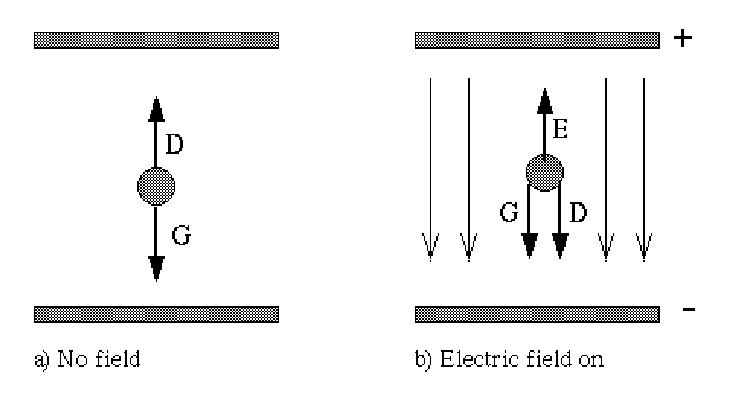
\epsfig{file=Introduction/oil_droplet.eps, height=5cm}
  \caption{
    Forces on an oil-droplet in: \newline
    \hspace*{1.5cm}
           a) Free fall          \newline
    \hspace*{1.5cm}
	   b) Electric field     \newline
    (G=Gravitation, D=Drag, E=Electric force)
  }
  \label{oil_droplet}
\end{center}
\end{figure}

His results were systematically low by about 4\% due to inaccurate
knowledge of the coefficient of viscosity. \newline
The electron charge is -e,
where $e = 1.602 \cdot 10^{-19}C$. All free particles are observed to
have values of electric charge equal to an integer times the
fundamental charge e:

\begin{equation*}
  q=n e
\end{equation*}

where the integer $n=\dots,-1,0,1,\dots$ is the electric charge
\emph{quantum number}.

\subsection*{The Nucleus}

In 1912, Ernest Rutherford and his associates discovered that the
positive charge of the atom is concentrated in a \emph{nucleus}. The
charge of the $\alpha$ particle, discovered by Becquerel, was
determined to be $2e$, and the mass of the $\alpha$ particle was
determined to be about four times the mass of the hydrogen
atom. \newline
A new particle with zero electric charge was discovered by bombarding
beryllium atoms with $\alpha$ particles. James Chadwick showed that
the new particle, the \emph{neutron}, had mass nearly equal to that of
the \emph{proton}.

\subsection*{The Bohr Model of the Atom}

In 1913, Niels Bohr made the first qunatitatively successful model of
the atom. Inspired by the work of Rutherford, Bohr made a planetary
model of the atom; with electrons moving in circular orbits about the
nucleus. This model may seem quite simple in retrospect, but for the
time it was a great advancement of science. In addition to the
classical circular orbits, the second part of Bohr's atomic model
contains a bold hypothesis of new physics. The new physics recognizes
that \emph{angular momentum} is \emph{quantized}; it can take only
certain values:

\begin{equation*}
  L = mvr = n \hbar
\end{equation*}

where $n$ is a positive integer. Solving the energy equations result
in orbits of radius:

\begin{equation*}
  r_n = \frac{n^2\hbar^2}{mke^2}
\end{equation*}

where the \emph{Bohr radius}

\begin{equation*}
  a_0 \equiv r_1 = \frac{\hbar^2}{mke^2} \approx 0.053 nm
\end{equation*}

is in the correct order of magnitude for the size of the atom!

{\bf Planc }





%               The Two First Excited states of Helium
\subsection{The Two First Excited states of Helium}

We will not make any calculations regarding exited states in this
thesis, but it is a really important issue in quantum mechanics. The
ground state energy does not tell much about the 
chemical properties of the atom on its own. Therefore good
approximations of the exited states are needed. Also, when discussing
different numerical approaches for solving the many body-problem,
including linear combinations of exited states may greatly improve
some original approximation to the ground state. Furthermore,
understanding how we include exited states is important for fully
understanding the application of the Slater determinant.
\newline
%
\newline
The state of helium with the $1s$ and the $2s$ orbitals occupied
with one electron each. 








The construction of the
periodic table in the second half of the $19^{\mathrm{th}}$ century
was based on the chemical properties of the different atoms. These
properties were not understood until the development of quantum
mechanics. The electrons are filled from the energetically lowest
orbitals. In the $s$ orbitals only two electrons of different
spins are allowed. Disregarding electron repulsion this would imply
that twice the energy is needed in removing an electron from ground
state helium than from the ground state hydrogen. This due to the 
double electric charge of the helium nucleus. The ionization energy of
hydrogen is $13.60 eV$ and the ionization energy of helium is $24.58
eV$ (ref. \cite{atkins2003}). The electron repulsion thus reduce the
ionization energy by almost $10\%$.
\newline
%
\newline
The early development of quantum theory may be summarized through the
four postulates of quantum mechanics.


%*************** The Postulates of Quantum Mechanics **************
%*
%*
\section{The Postulates of Quantum Mechanics}

A common formulation of quantum mechanics is by means of linear
algebra. In this formulation every state is represented as a (usually
infinite dimensional) complex vector, and an operator is represented
as a complex, linear and hermitian matrix. 
The postulates of quantum mechanics fall naturally into two sets: the
first three, which tell us how the system is depicted at a given time,
and the fourth, which specifies how this picture changes with time. 
\newline

%*                     The First Postulate                              *
%\subsection{The First Postulate}

{\bf \large Postulate 1}
\emph{
The state of a quantum mechanical particle is described by a vector
$\Psi$ in a Hilbert space ${\cal H}$. All the possible states of the
particle are ${\cal H}$ except the zero vector.
\newline
}

The first postulate states that a particle is described as a vector in
the Hilbert space. So a particle with finite degrees of
freedom $\mathbf{x}$ and $\mathbf{p}$ in classical
mechanics, now has infinite degrees of freedom. 
\newline

%*                     The Second Postulate                              *
%\subsection{The Second Postulate}

{\bf \large Postulate 2}
\emph{
Every observable are represented by an Hermitian linear operator in
${\cal H}$. For every classical dynamical variable
$\omega(\mathbf{x},\mathbf{p})$ there is a corresponding quantum
mechanical operator $\Omega$  obtained by operator substitution of the
fundamental position and momentum operators $\mathbf{X}$ and
$\mathbf{P}$, respectively: 
}
%
\begin{equation*}
  \Omega(\mathbf{X},\mathbf{P}) = \omega(\mathbf{x} \to
  \mathbf{X},\mathbf{p} \to \mathbf{P})
\end{equation*}
%
\emph{
The components of $\mathbf{X}$ and $\mathbf{P}$ are operators defined
through the fundamental commutation relation
}

\begin{equation*}
  \left[ X_i, P_j \right] = i \hbar \delta_{ij}
\end{equation*}

The second postulate tell us how to to move from the classical to the
quantum mechanical picture. The observables (or measurable quantities)
are defined through an operator. This operator may be obtained by
simple substitution of the position and the momentum of the
corresponding classical observable.
\newline

%*                     The Third Postulate                              *
%\subsection{The Third Postulate}

{\bf \large Postulate 3}
\emph{
The only possible values obtainable in an (ideal) measurement of an
observable $\Omega$ are its eigenvalues $\omega_n$. Each have a
probability
}
%
\begin{equation*}
  P(\omega_n) = \frac{\int \Psi^* \Phi_n }{\int \Psi^* \Psi }
\end{equation*}
%
\emph{
with $\Phi_n$ the eigenfunction corresponding to the eigenvalue
$\omega_n$. Immediately after a measurement the state collapses into
$\Phi_n$.
}
\newline

The third postulate tells what may be extracted from the quantum
mechanical picture by means of measurements. Note that the eigenvalues
may either have a continuous spectrum or be \emph{quantized}.
\newline


%*                     The Fourth Postulate                              *
%\subsection{The Fourth Postulate}

{\bf \large Postulate 4}
\emph{
The time development of the quantum state $\Psi$ is given by the time
dependent Schr\"odinger equation,
}

\begin{equation*}
  \hat{H} \Psi(\mathbf{x},t) = i\hbar \frac{\delta}{\delta
  t}\Psi(\mathbf{x},t) 
\end{equation*}

The fourth and final postulate defines the Schr\"odinger
equation. This equation describes how the quantum mechanical state
evolve in time.
\newline





\part{Theory}
\chapter{Quantum mechanics}
\label{ch:qm}
During a period spanning more that 50 years, from the end of the 19th century till the late twenties in the previous century, several discoveries were made that could not be properly explained by the by then available theoretical approaches based on for example Newtonian mechanics.
Phenomena like the photoelectric effect, blackbody radiation, Compton scattering, X-rays etc. were all processes which required a finer resolution of scales, leading eventually to the theory of quantum mechanics and its postulates, with Schr\"odinger's equation being the new mathematical framework to express the laws of motion at nano or smaller scales.  
%MHJ forandring
%the beginning of the 20th century a new era in physics was rising.
%A number of discoveries, that were inconsistent with the classical laws of physics, had been found during the last years.
%In order to explain these inconsistencies, a new theory had to be derived, leading to what is now known as quantum mechanics.
%In contrast to many earlier theories, as Newtonian mechanics and Maxwell's equations, to mention a few, quantum mechanics has been developed in collaboration by many persons.
%This approach to develop a new theory lead to both agreements and disagreements, and one can still see signs of a difficult youth, but over the years it has stabilized into a more consistent theory.



\section{Fundamentals}
Objects in classical mechanics have well-defined positions, which can
be tracked over a time interval by Newton's laws of motion.
Once we know the initial state and all forces present, we can predict the
motion of objects until the end of time. 
It is of course not doable in practice, because we cannot know \textit{all variables}, and certainly not to \textit{endless accuracy}. 
We say that Newtonian mechanics is a deterministic theory.
Quantum mechanics, with its postulates like its matter-wave duality and Heisenberg's uncertainty principle, introduces an approach to describe Nature that represents a probabilistic determinism. 
In this chapter we discuss some of the basic tools and postulates needed to describe physical systems governed by Schr\"odinger's equation.
%MHJ retting
%It holds on to the concept of all matter being waves, with an extent in space,
%and thus also a built-in uncertainty.
%We could never know exactly where a particle is.


\subsection{The wave function}
We begin with only one electron floating in empty space.
To describe this electron we would construct a so-called wave function,
typically written as $\Psi(\vec{r},t)$.
If the particle is influenced by some external potential energy $V$, we could find
the time evolution by solving the Schrödinger equation,
\begin{equation}
\label{eq:qm:schrodinger}
i\hbar \frac{\partial \Psi}{\partial t} = - \frac{\hbar^2}{2m}
\nabla^2 \Psi+ V \Psi .
\end{equation}
It is common to simplify this by defining the Hamiltonian operator,
\begin{equation}
\hat{H} = \hat{T} + \hat{V},
\end{equation}
where $\hat{T}$ is the operator of kinetic energy,
\begin{equation}
\hat{T} = \frac{\hat{p}^2}{2m} = - \frac{\hbar^2}{2m} \nabla^2,
\end{equation}
and $\hat{V}$ is the potential. 
Our Hamiltonian thus represents the total energy for this particle.
It is now possible to rewrite the full Schrödinger equation as
\begin{equation}
\label{eq:qm:schrodingersimple}
i\hbar \frac{\partial \Psi}{\partial t} = \hat{H} \Psi .
\end{equation}
The Schrödinger equation serves as an analog to Newton's laws.
If the initial conditions for $\Psi$ and the exact potential $\hat{V}$ are known, 
we could calculate the wave function for any time later.
All solutions of the Schrödinger equation reside in what is known as the Hilbert
space.


\paragraph*{}
A physicist's first attempt at solving partial differential equations is to see whether the technique of separation of variables can be applied or not.
We assume that the potential $\hat{V}$ is time independent and the solutions consist of a time-independent factor $\psi$, and another factor depending only on time, $\tau$.
If multiple such products are solutions, then it is clear that any linear
combination of these products is a solution too.
Thus,
\begin{equation}
\label{eq:qm:linearComb}
\Psi(\vec{r},t) = \sum_n c_n \psi_n(\vec{r}) \tau_n(t).
\end{equation}
After inserting one term from \eqref{eq:qm:linearComb} into \eqref{eq:qm:schrodinger}, we separate the two factors to appear on
differing sides,
\begin{equation}
\frac{i\hbar}{\tau_n(t)} \frac{\partial \tau_n(t)}{\partial t} =
E_n =
- \frac{\hbar^2}{\psi_n(\vec{r}) 2m} \nabla^2 \psi_n(\vec{r}) + \hat{V} .
\end{equation}
Here, $E_n$ is a constant of separation, and we should note that this may fail
if our Hamiltonian has some explicit time dependency.
We can solve this for $\tau_n$, yielding
\begin{equation}
\frac{d\tau_n(t)}{dt} = \frac{E_n}{i\hbar} \tau_n(t)
\Rightarrow
\tau_n(t) = e^{-\frac{i}{\hbar}E_n} .
\end{equation}
It is necessary to solve the time-independent Schrödinger
equation in order to find $\psi_n$,
\begin{equation}
\label{eq:qm:schrodingernotime}
- \frac{\hbar^2}{2m} \nabla^2 \psi_n(\vec{r}) + \hat{V} \psi_n(\vec{r}) = E_n
\psi_n(\vec{r})
\Rightarrow
\hat{H} \psi_n(\vec{r}) = E_n \psi_n(\vec{r}) .
\end{equation}
The Hamiltonian operator, $\hat{H}$, represents the energy of the wave function it is acting upon.
It is thus clear why the constant of separation was called $E_n$.


\paragraph*{}
With the knowledge on how to find the wave function at any time for a
specific potential, it is still not obvious what the interpretation of a wave
function is, yet more unclear how one can extract observable quantities from
this construct.

The wave function is a complex function, describing the spatial distribution of a particle.
Born's statistical interpretation states that the probability of finding a
particle in a region $\Omega$ at a time $t$, is
\begin{equation}
\int_{\Omega} \Psi^{*}(\vec{r},t) \Psi(\vec{r},t) d^3\vec{r} .
\end{equation}
In order for this to be correct it is customary to work with normalized wave
functions, that is, scaling $\Psi$ with a complex 
constant\footnote{Another possibility is to work
with unnormalized wave functions, and always divide these type of integrals by
$\int_{-\infty}^{\infty} \left| \Psi(\vec{r},t) \right|^2 d^3\vec{r}$.}
to enforce that
\begin{equation}
\int_{-\infty}^{\infty} \left| \Psi(\vec{r},t) \right|^2 d^3\vec{r} = 1 .
\end{equation}
Loosely speaking this enforces that if the particle exists it has to be somewhere, and the probability to find it if we look everywhere has to be $1$.
The concept of not knowing where the particle is leads to many fundamental
questions, both physical and philosophical.
As most of these questions lead to an endless discussion with no clear answer
(yet), we will not try to answer them here. 

\paragraph*{}
In addition to the spatial distribution varying in time, particles have an intrinsic property, possessing a magnetic dipole moment, known as spin.
Despite acting similarly to a charged rotating body in classical electrodynamics, elementary particles have no known inner structure, making it a different phenomenon.
Spin is quantized, as many other properties in quantum mechanics, and should be accounted for in the wave function by multiplication of a spin part, $\chi$.
Electrons, which form the key focus in this study, have a spin quantum number $s = \frac{1}{2}$ that can be projected in two directions, $\pm\frac{1}{2}$, often referred to as up and down.
In fact all spatial wave functions in this chapter, $\psi$, should then have a total \textit{spin-orbital} 
\begin{equation}
\psi \chi_{\downarrow} \textrm{ or } \psi \chi_{\uparrow} .
\end{equation}
Degeneracies, multiple particles and spin dependent Hamiltonians can complicate our theory somewhat, but neither of these effects are encountered in this chapter.



\subsection{Observables}
%MHJ
% trengs ikke, gaa rett paa sak
%Preparing multiple equal systems in the same state, having the same wave function, and performing equal measurements on all of them under the same conditions, the measurements can yield different results on the different systems.\footnote{Note the difference between measuring on multiple equal systems and doing multiple measurements on the same system. Doing a measurement on any system will alter its state, leading to a different state in the next measurement.}
%One therefore often work with the expectation value, which is the average of all outcomes on equal systems, not to be confused with the expected, most likely result.
%\paragraph*{}

In quantum mechanics observables are represented by operators.
As all measurements must have a real value, all such operators need to return real expectation values.
The expectation value of an observable with an operator $\hat{O}$ is calculated
as\footnote{Here, and when convenient from now on, we will skip the integration 
limits and stick to $dx$ to denote an integral over all space 
spanned by all variables of freedom.}
\begin{equation}
\label{eq:qm:expectation}
\langle \hat{O} \rangle = \int \Psi^{*} \hat{O} \Psi dx .
\end{equation}
With the expectation value being real; 
$\langle \hat{O} \rangle = \langle \hat{O} \rangle^{*}$, and therefore also
\begin{equation}
\label{eq:qm:hermitian}
\int \Psi^{*} \hat{O} \Psi dx 
= \left(\int \Psi^{*} \hat{O} \Psi dx\right)^{*}
= \int \left(\hat{O} \Psi\right)^{*} \Psi dx .
\end{equation}
All operators for observables will need to possess this property when acting on any wave function, $\Psi$, within the Hilbert space, referred to as Hermitian or self-adjoint operators.
There are two fundamental examples of operators representing physical observables, position and momentum. 
The position has the simplest correspondence,
\begin{equation}
\label{eq:qm:operX}
\hat{x} = x,
\end{equation}
whereas momentum is represented as
\begin{equation}
\hat{p} = - i \hbar \nabla .
\end{equation}
Other quantities can be derived from the position and momentum operators using a
reasoning close to classical quantities, e.g. kinetic energy,
\begin{equation}
\hat{T} = \frac{1}{2} m \hat{v}^2 = \frac{\hat{p}^2}{2m} = - \frac{\hbar^2}{2m} \nabla^2 .
\end{equation}


\subsection{The canonical commutation relation}
\label{sec:qm:commutator}
Similar to matrices in linear algebra, not all operators commute.
Having two operators $\hat{A}$ and $\hat{B}$, the order of which they are applied may affect the result, thus in general
\begin{equation}
\hat{A}\hat{B} \neq \hat{B}\hat{A} .
\end{equation}
One typically defines the commutator
\begin{equation}
\label{eq:qm:commutator}
[\hat{A}, \hat{B}] = \hat{A}\hat{B} - \hat{B}\hat{A} ,
\end{equation}
having the properties listed below:
\begin{enumerate}[{\bf a. }]
\item Switching order between the two operators changes the sign,
\begin{equation}
[\hat{A}, \hat{B}] = - [\hat{B}, \hat{A}] .
\end{equation}
\item All constants can safely be placed in front of the commutator, 
\begin{equation}
[c_a \hat{A}, c_b\hat{B}] = c_a c_b [\hat{A}, \hat{B}] .
\end{equation}
\item Summation of two operators inside one commutator can be carried out as a sum of two commutators,
\begin{equation}
[\hat{A}, \hat{B} + \hat{C}] = [\hat{A}, \hat{B}] + [\hat{A}, \hat{C}] .
\end{equation}
\end{enumerate}
These properties follow directly from the definition \eqref{eq:qm:commutator}. 
More properties can be derived, but we restrict us to the properties of interest later in this thesis.
%TODO Describe where it is of value???

Even the operators for position and momentum do not commute in quantum mechanics, a fact that can be shown in a few steps.
To make the derivation conceptually easier we let the operators act on an arbitrary test function $\Psi_T$, and concentrate on one dimension, i.e.
\begin{equation}
[\hat{x}, \hat{p}] \Psi_T = -i\hbar [\hat{x}, \frac{\partial}{\partial x}] \Psi_T 
= -i \hbar \left( \hat{x} \frac{\partial}{\partial x} \Psi_T - \frac{\partial}{\partial x}\left(\hat{x} \Psi_T \right) \right) .
\end{equation}
Applying the product rule on the last term we end up with
\begin{equation}
-i \hbar \left( \hat{x} \frac{\partial}{\partial x} \Psi_T - \Psi_T 
- \hat{x} \frac{\partial}{\partial x} \Psi_T \right)
= i\hbar \Psi_T .
\end{equation}
Dropping the test function, we have proved what is known as the canonical commutation relation,
\begin{equation}
\label{eq:qm:canonicalcommutation}
[\hat{x}, \hat{p}] = i\hbar .
\end{equation}



\subsection{Eigenfunctions}
Letting an observable $\hat{O}$ act on a state $\Psi$, one may get different
results, each with its own probability.
This \textit{spectra} of results can be either continuous or discrete, and it is of interest to know if a state yielding the same value each and every time for an operator can be found.
In fact such states exist, and one is already encountered in the time-independent Schrödinger equation, (\ref{eq:qm:schrodingernotime}), where a state $\psi_n$ will return the energy $E_n$ when acted upon by $\hat{H}$.
Such states are called eigenstates, having a corresponding eigenvalue.
For any observable, its eigenstates are found by the eigenvalue equation,
\begin{equation}
\label{eq:qm:eigenvalue}
\hat{O} \psi_n = O_n \psi_n .
\end{equation}
A few properties for such functions can be proven:
%MHJ  har du referanse her?
\begin{itemize}
\item All eigenvalues of a Hermitian operator are real.

Using the property of Hermitian operators from eq.~\eqref{eq:qm:hermitian}, we have
\begin{equation}
\int \psi_n^{*} \hat{O} \psi_n dx 
= \int \left(\hat{O} \psi_n\right)^{*} \psi_n dx 
\Rightarrow
O_n \int \psi_n^{*} \psi_n dx 
= O_n^{*} \int \psi_n^{*} \psi_n dx ,
\end{equation}
which means $O_n = O_n^{*}$, and thus real.

\item Different eigenfunctions are orthogonal.

Another form of the condition for Hermitian operators is
\begin{equation}
\int \psi_m^{*} \hat{O} \psi_n dx 
= \int \left(\hat{O} \psi_m\right)^{*} \psi_n dx .
\end{equation}
Despite looking like a stronger condition it is in fact equivalent with eq.~\eqref{eq:qm:hermitian} \cite{griffiths}, resulting in 
\begin{equation}
O_n \int \psi_m^{*} \psi_n dx 
= O_m^{*} \int \psi_m^{*} \psi_n dx .
\end{equation}
Since it is already known that the eigenvalues are real there is no other
possibility than $\int \psi_m^{*} \psi_n dx = 0$ whenever $O_n \neq O_m$.

\item For any operator with a finite set of eigenfunctions, the eigenfunctions
are complete. They span the Hilbert space, such that any function in this space
can be expressed as a linear combination of eigenfunctions.
%TODO strange! 
It can, in fact, not be proven in general for spectra with infinite number of eigenstates.
Nonetheless, it is taken as a necessity, and thus a restriction on the observable operators.
\end{itemize}



\subsection{Bra-ket notation}
In daily work the wave functions encountered are seldom written as explicit functions.
One typically refer to states instead, hiding the complexity of dealing with
functions and integrals, into constructs called `bra' and `ket'.
Dirac introduced this notation in 1930, and named it after splitting the word
`bracket'~\cite{bracket}.

\paragraph*{}
A ket state is the right-hand part, where a state $\Psi$ would be represented as $|\Psi \rangle$.
This represents a particle, with a corresponding
wave function.
The ket state can be viewed as a column vector,
\begin{equation}
\label{eq:qm:bra}
|\Psi \rangle = 
\begin{bmatrix}
c_0 \\
c_1 \\
c_2 \\
... \\
\end{bmatrix}
\textrm{ or }
|\Psi \rangle =
\begin{bmatrix}
\Psi(x_0) \\
\Psi(x_1) \\
\Psi(x_2) \\
... \\
\end{bmatrix} ,
\end{equation}
where the first example has $\Psi$ in a state with a given basis for a \textit{finite} Hilbert space.
The other example has the ket state represented in an \textit{infinite} Hilbert space, as there are
infinitely many positions $x_i$.

\paragraph*{}
The bra state is the left-hand part of the bracket, referred to as the ket's dual, being the Hermitian transposed\footnote{Hermitian transposed means the transposed vector, where the complex conjugate is performed on each element.} of corresponding ket.
Following the first example in eq.~\eqref{eq:qm:bra} the bra state would be
\begin{equation}
\langle \Psi | =
\begin{bmatrix}
c_0^{*}, c_1^{*}, c_2^{*}, ... \\
\end{bmatrix}.
\end{equation}
The expectation values of operators can then be viewed as matrices.
This is just a picture, as 
most of the vectors will be in infinite dimensional spaces explained by
functions.
The notation will, however, give us a linear algebra like syntax, a formalism
that ease our daily work.
Operators will in this syntax work in the same way as for wave functions.
The dual part of an operator acting from the left on a ket state, will be the operator's Hermitian adjoint acting from the right on a bra state,
%TODO vanskelig forklart?
\begin{equation}
\hat{O}|\Psi \rangle  \longleftrightarrow  \langle \Psi | \hat{O}^{\dagger} .
\end{equation}

\paragraph*{}
Having introduced these brackets, it is time to define a particularly useful
operation, the inner product.
The definition is straight forward in a linear-algebra sense, except that we need to  extended it to an infinite space by the integral 
\begin{equation}
\langle \Psi_i | \Psi_j \rangle =
\int \Psi_i^{*} \Psi_j dx .
\end{equation}
Operators can be placed in between the bra and the ket states, reducing the expectation value
from \eqref{eq:qm:expectation} to
\begin{equation}
\langle \hat{O} \rangle = 
\langle \Psi | \hat{O} | \Psi \rangle .
\end{equation}
The fact that observable operators are Hermitian can now be simplified from
\eqref{eq:qm:hermitian} to 
\begin{equation}
\langle \Psi | \hat{O} | \Psi \rangle = \langle \Psi | \hat{O}^{\dagger} | \Psi \rangle,
\end{equation}
where $\hat{O} = \hat{O}^{\dagger}$ is referred to as self-adjoint.



\subsection{A fundamental summary}
The new syntax of bra-ket notation allows us to summarize quantum mechanics into a
few neatly expressed postulates. 
Although these postulates are presented in a slightly different manner by
different authors, the main concepts can be put into four postulates:
\begin{enumerate}[{Postulate} 1: ]
\item The state of an isolated physical system can be described by a
state-vector, $|\Psi \rangle$,  within
a Hilbert space, $\mathcal{H}$.
\item Every physical observable, $O$, has a corresponding linear Hermitian
operator, $\hat{O}$, acting on vectors in $\mathcal{H}$.
\item A measurement of the quantity $O$, with a corresponding operator
$\hat{O}$, is guaranteed to yield one of the operator's eigenvalues, $O_n$, with a
certain probability.
\item The state-vector has a time evolution satisfying the Schrödinger
equation,
\begin{equation}
\label{eq:qm:schrodingerbraket}
i\hbar \frac{\partial}{\partial t} | \Psi(t) \rangle =
\hat{H} | \Psi(t) \rangle .
\end{equation}
\end{enumerate}



\section{Harmonic oscillator}
\label{sec:qm:ho}
In this section we will calculate, using the fundamental theory from previous section, the energy spectra along with its eigenstates for a system that is simple, but of high interest.
The problem to solve in this thesis is the harmonic oscillator in two dimensions, but
to begin with we will only treat the one dimensional problem, ending up with
solutions for two dimensions at no extra cost.

\paragraph*{}
A classical harmonic oscillator consists of a particle attached to a spring.
The farther the particle moves, the larger the force from the spring, according
to Hooke's law,
\begin{equation}
F = -kx .
\end{equation}
A potential field $V$ is simply the negative of the work done, and using this relation, we can calculate the potential energy as a simple integral,
\begin{equation}
V = - \int_0^x -kx dx = \frac{1}{2} kx^2 = \frac{1}{2} m \omega^2 x^2,
\end{equation}
where $\omega = \sqrt{k/m}$ is called the frequency.
This can be inserted into the Hamiltonian by replacing $x$ with its quantum
mechanical operator, found in eq.~\eqref{eq:qm:operX}. The total Hamiltonian reads 
$-\frac{\hbar^2}{2m}\frac{d^2}{dx^2} + \frac{1}{2} m \omega^2 x^2$, leading to
the time-independent Schrödinger equation
\begin{equation}
-\frac{\hbar^2}{2m}\frac{d^2}{dx^2}|\psi_n\rangle + \frac{1}{2} m \omega^2 x^2|\psi_n\rangle 
= E_n|\psi_n\rangle .
\end{equation}
It may be tempting to attack this problem in a brute force manner.
That would however prove quite tedious, and better strategies exist.


\subsection{The ladder operators}
\label{sec:qm:ladder}
Following an, at first, unexpected path, we will introduce what is known as the ladder, or excitation, operator, defined by
\begin{equation}
\hat{a}^{\dagger} = \sqrt{\frac{m\omega}{2\hbar}} \left(\hat{x} - \frac{i\hat{p}}{m\omega} \right) ,
\end{equation}
and its Hermitian adjoint, the de-excitation operator\footnote{One can prove that the excitation and de-excitation operators are the Hermitian adjoint of each other. It will however serve no purpose to us at this stage.},
\begin{equation}
\hat{a} = \sqrt{\frac{m\omega}{2\hbar}} \left(\hat{x} + \frac{i\hat{p}}{m\omega} \right) .
\end{equation}
The motivation for selecting these two operators may seem unclear, but their product is of interest,
\begin{equation}
\hat{a}\hat{a}^{\dagger} = 
\frac{m\omega}{2\hbar} \left(\hat{x}^2 + \frac{i}{m\omega}[\hat{p},\hat{x}] + \frac{\hat{p}^2}{m^2 \omega^2} \right) =
\frac{m\omega}{2\hbar} \hat{x}^2 + \frac{\hat{p}^2}{2\hbar m \omega} + \frac{i}{2\hbar} [\hat{p},\hat{x}] ,
\end{equation}
where the first two terms are found in the Hamiltonian, and the last term can be expressed by the canonical commutation relation~\eqref{eq:qm:canonicalcommutation},
\begin{equation}
\hat{a}\hat{a}^{\dagger} = 
\frac{1}{\hbar \omega} \hat{H} + \frac{1}{2} \Rightarrow
\hat{H} = \hbar \omega \left( \hat{a}\hat{a}^{\dagger} - \frac{1}{2} \right) .
\end{equation}

Being able to rewrite our Hamiltonian, it is tempting to investigate these operators further. In particular, it is of interest to find their commutator.
Using the rules of commutators shown in section~\ref{sec:qm:commutator} we find,
\begin{equation}
[\hat{a},\hat{a}^{\dagger}] = 
\frac{m \omega}{2\hbar} \left[\left( \hat{x} + \frac{i\hat{p}}{m \omega} \right), \left(\hat{x} - \frac{i\hat{p}}{m \omega} \right) \right] =
\frac{m \omega}{2\hbar}  [\hat{x},\hat{x}] + \frac{i}{\hbar}[\hat{p},\hat{x}] + \frac{1}{2\hbar m\omega} [\hat{p},\hat{p}] ,
\end{equation}
where only the second term is nonzero,
\begin{equation}
[\hat{a},\hat{a}^{\dagger}] = 
\frac{i}{\hbar}[\hat{p},\hat{x}] = 
-\frac{i}{\hbar} i \hbar =
1 .
\end{equation}
Because of this, the Hamiltonian can equally well be written in one out of two forms,
\begin{equation}
\label{eq:qm:hohamiltonian}
\hat{H} = \hbar \omega \left( \hat{a}\hat{a}^{\dagger} - \frac{1}{2} \right)
\textrm{ or }
\hat{H} = \hbar \omega \left( \hat{a}^{\dagger}\hat{a} + \frac{1}{2} \right).
\end{equation}

\paragraph*{}
The crucial step comes when claiming that one, yet unknown, state, $|\psi_n \rangle$, is a solution of the time-independent Schrödinger equation, $\hat{H} |\psi_n \rangle = E_n |\psi_n \rangle$.
With this in mind, one may ask what the energy of $\hat{a}^{\dagger} |\psi_n\rangle$ is, 
\begin{equation}
\begin{split}
\hat{H}\left(\hat{a}^{\dagger}|\psi_n \rangle\right) &= 
\hbar \omega \left(\hat{a}^{\dagger}\hat{a}\hat{a}^{\dagger} + \frac{1}{2}\hat{a}^{\dagger} \right) |\psi_n \rangle = 
\hbar \omega \hat{a}^{\dagger} \left(\hat{a}\hat{a}^{\dagger} + \frac{1}{2} \right)|\psi_n \rangle \\
&= \hbar \omega \hat{a}^{\dagger} \left(\hat{a}^{\dagger}\hat{a} + 1 + \frac{1}{2} \right)|\psi_n \rangle 
= \hat{a}^{\dagger} \left(\hat{H} +\hbar \omega  \right)|\psi_n \rangle 
= \left(E_n +\hbar \omega  \right)\hat{a}^{\dagger}|\psi_n \rangle .
\end{split}
\end{equation}
The last steps were achieved by exploiting the commutator between the excitation and de-excitation operator, and then recall that $|\psi_n \rangle$ is an eigenstate of $\hat{H}$.
With the same approach one would also find that 
\begin{equation}
\hat{H}\left( \hat{a} |\psi_n \rangle \right) =
\left(E_n - \hbar \omega \right) \hat{a}|\psi_n\rangle .
\end{equation}
With these operators we have the possibility to create states with energy at discrete steps of $\hbar \omega$, as long as we find at least one state to start out with. It seems reasonable that there should exist a lower limit, where applying $\hat{a}$ should give us no new state, viz.
\begin{equation}
\hat{a} |\psi_0 \rangle = 0 .
\end{equation}
For convenience it is possible to label this state simply $|0\rangle$.
By inserting the full expression for $\hat{a}$ and solving the differential equation,
\begin{equation}
\begin{split}
\sqrt{\frac{m\omega}{2\hbar}} \left(\hat{x} + \frac{i}{m\omega}\left(-i\hbar \frac{\partial}{\partial x} \right)\right) &|0\rangle = 0
\Rightarrow 
\int \frac{d |0\rangle}{|0\rangle} = -\frac{m\omega}{\hbar}\int x dx
\\ \\ \Rightarrow 
&|0\rangle = C e^{-\frac{m\omega}{2\hbar} x^2} ,
\end{split}
\end{equation}
we get an explicit expression for the lowest-lying state, up to a constant $C$ to be determined by normalization.

\paragraph*{}
The only remaining task is to find the energy of the ground state, $E_0$.
Inserting expression~\eqref{eq:qm:hohamiltonian} for the Hamiltonian into the time-independent equation, we find
\begin{equation}
\hbar\omega \left( \hat{a}^{\dagger}\hat{a} + \frac{1}{2} \right) | 0 \rangle
= \hbar\omega  \hat{a}^{\dagger}\hat{a} |0\rangle + \frac{1}{2}\hbar\omega | 0 \rangle = E_0 |0\rangle .
\end{equation}
But since $\hat{a}|0\rangle = 0$, it is clear that $E_0 = \frac{1}{2}\hbar\omega$, and using the fact that eigenstates exist at steps of $\hbar \omega$, the complete energy spectrum is 
\begin{equation}
E_n = \left( n + \frac{1}{2} \right) \hbar \omega .
\end{equation}



\subsection{Two dimensions}
\label{sec:qm:ho2d}
So far, we have treated the oscillator problem in only one dimension.
Moving to two dimensions, the actual Hamiltonian of interest changes to
\begin{equation}
\hat{H}
= -\frac{\hbar^2}{2m}\nabla^2 + \frac{1}{2} m \omega^2 r^2  
= -\frac{\hbar^2}{2m}\left(\frac{\partial^2}{\partial x^2} +\frac{\partial^2}{\partial y^2} \right) + \frac{1}{2} m \omega^2 \left(x^2 + y^2\right) .
\end{equation}
Once again we will, as physicists, attack this by separation of variables, assuming that the new state $|n\rangle$ is a product of independent states in $x$ and $y$,
\begin{equation}
|n\rangle = |n_x \rangle \otimes |n_y \rangle .
\end{equation}
It is already clear that $\hat{H}$ can be written as a sum of two Hamiltonians, where each is only one dimensional,
\begin{equation}
\hat{H} = \hat{H_x} + \hat{H_y} 
= \left(-\frac{\hbar^2}{2m}\frac{\partial^2}{\partial x^2} + \frac{1}{2} m \omega^2 x^2\right) + \left(-\frac{\hbar^2}{2m}\frac{\partial^2}{\partial y^2}  + \frac{1}{2} m \omega^2 y^2\right) .
\end{equation}
The total time-independent Schrödinger equation now reads
\begin{equation}
\hat{H}|n\rangle = \left(\hat{H_x}|n_x \rangle \right) \otimes |n_y \rangle + |n_x \rangle \otimes \left( \hat{H_y} |n_y \rangle \right)
= E_n \left( |n_x \rangle \otimes |n_y \rangle \right),
\end{equation}
and since $H_x$ has the eigenstates found by using the ladder operators, with energies $E_{n_x} = \left(n_x + \frac{1}{2} \right) \hbar\omega$, the total energy is
\begin{equation}
E_{n_x,n_y} 
= \left(n_x + \frac{1}{2}\right) \hbar \omega + \left(n_y + \frac{1}{2}\right) \hbar \omega
= \left(n_x + n_y + 1\right) \hbar \omega .
\end{equation}

\paragraph*{}
Understanding the methods here, with the ladder operators, has a great value.
When moving on to many-body methods, similar constructs, called creation and annihilation operators, will be used to simplify calculations.
Whereas the ladder operators simply `moved' the electron to a state with a different energy, the creation and annihilation operators will add or remove electrons from a system.














\chapter{Many-body theory}
It is often insufficient to be able to calculate properties in systems with only one particle.
One would for example be restricted to only hydrogen, if studying atoms.
Methods for many-particle systems have thus been developed, often theoretically exact, but in practice we must rely on computer programs having a truncation affecting the accuracy of the results.
Different types of approximations, or many-body methods, exists, where widely
used techniques are; configuration interaction, perturbation theory, Hartree-Fock, Monte-Carlo methods and coupled-cluster theory.
Even though we will focus mainly on the coupled-cluster approach, the concepts from this chapter are typically the same for all the different methods.


\section{The non-interacting case}
The natural starting point for many-body theory is to deal with non-interacting particles.
In this case the Schrödinger equation holds the same form now as it did for one particle in eq. \eqref{eq:qm:schrodingerbraket}.
Assuming a time-independent Hamiltonian,
\begin{equation}
\hat{H} = \sum_k \hat{h}_k =  \sum_k \hat{t}_k  + \sum_k \hat{v}_k ,
\end{equation}
with $\hat{t}_k$ and $\hat{v}_k$ being the operators for kinetic and potential energy for particle $k$, the energy is constant in time and we only need to solve the time-independent Schrödinger equation.
Since the particles are not interacting, this equation is separable, and we assume a total wave function, $|\Psi^{(\lambda)} \rangle$, being a product of different single-particle spin orbitals $|\psi_k^{(\lambda)}\rangle$, with a total energy $E^{(\lambda)}=\sum_k E_k^{(\lambda)}$,
\begin{equation}
\hat{H}|\Psi^{(\lambda)} \rangle = 
\left(\sum_k \hat{h}_k\right) \left(|\psi_1^{(\lambda)}\rangle \otimes |\psi_2^{(\lambda)}\rangle 
\cdots \otimes |\psi_N^{(\lambda)}\rangle \right)
=  \sum_k E_k^{(\lambda)} |\Psi^{(\lambda)} \rangle .
\end{equation}
Here $E_k^{(\lambda)}$ is the energy of particle $k$, satisfying the single-particle eigenvalue equation,
\begin{equation}
\label{eq:manybody:nonInter}
\hat{h}_k |\psi_k^{(\lambda)} \rangle = E_k^{(\lambda)} |\psi_k^{(\lambda)} \rangle .
\end{equation}
It is important to note how the subscript refers to the different particles, whereas the superscript denotes different eigenstates inside a spectrum of energies.

Electrons are, although it complicates our calculations, interacting through the coulomb repulsion. 
For this reason we keep this simple separable calculation in memory when we move on to many-body theory which yields the correlation as a correction to the non-interacting reference energy.


\section{Indistinguishable and identical particles}
An important aspect when considering systems with more than one particle is that electrons are not only identical, they are in fact indistinguishable.
In quantum mechanics it makes no sense talking about different particles, they are truly identical and impossible to track one at a time.
As a consequence of this, interchanging the coordinates of two particles should not alter the probability distribution, i.e.
\begin{equation}
\label{eq:manybody:interchange}
| \Psi |^2
=
|\hat{P}_{ij} \Psi |^2 .
\end{equation}
This compact notation is due to the introduction of the permutation operator $\hat{P}_{ij}$, interchanging particle $i$ and $j$. Equation~\eqref{eq:manybody:interchange} holds only if
\begin{equation}
\hat{P}_{ij} = \pm 1 ,
\end{equation}
where particles with a symmetric wave function, that is $\hat{P}_{ij} = 1$, are called bosons, while particles having an antisymmetric wave function, $\hat{P}_{ij} = -1$, are called fermions.

\paragraph*{}
Since electrons are fermions we need to construct wave functions that are antisymmetric.
The simple product we assumed in the non-interacting case is insufficient.
Antisymmetric wave functions are usually expressed as determinants, as proposed by John C. Slater, therefore called Slater determinants \cite{PhysRev.34.1293}.
Having a complete, orthonormal, single-particle basis where $N$ functions,  $\phi_{\alpha}, \phi_{\beta}, \cdots \phi_{\delta}$, are occupied by $N$ particles at different positions, $\vec{r_1}, \cdots , \vec{r_N}$, a $N$-particle wave function reads
\begin{equation}
\label{eq:manybody:slater}
\Phi_{\alpha,\beta,\cdots,\delta}(\vec{r_1},\cdots,\vec{r_N})
=
\frac{1}{\sqrt{N!}}
\left|
\begin{matrix}
\phi_{\alpha}(\vec{r_1}) & \phi_{\beta}(\vec{r_1}) & \cdots & \phi_{\delta}(\vec{r_1}) \\
\phi_{\alpha}(\vec{r_2}) & \phi_{\beta}(\vec{r_2}) & \cdots & \phi_{\delta}(\vec{r_2}) \\
\vdots                   & \vdots                  & \ddots & \vdots \\
\phi_{\alpha}(\vec{r_N}) & \phi_{\beta}(\vec{r_N}) & \cdots & \phi_{\delta}(\vec{r_N})\\
\end{matrix}
\right| .
\end{equation}
The notation here is of importance.
Up to now we have looked at the exact solution, denoted $\Psi$.
In this step the single particle basis $\phi$ can be any complete basis, and therefore $\Phi$ is in general not the exact solution.
The solution can however be expressed as a combination of slater determinants, 
\begin{equation}
|\Psi^{(\lambda)} \rangle = 
\sum_{\alpha,\beta,\cdots,\delta} C_{\alpha,\beta,\cdots,\delta}^{(\lambda)}
|\Phi_{\alpha,\beta,\cdots,\delta} \rangle ,
\end{equation}
due to the completeness of our basis functions.
Determinants have the property of being zero whenever two columns are equal.
This is a manifestation of the exclusion principle formulated by Wolfgang Pauli in 1925~\cite{springerlink:10.1007/BF02980631}, two fermions can not share the same state, which he later received the Nobel prize for in 1945.
Including the two spin states available for each electron, no more than two electrons can share the same orbital.

\paragraph*{}
To incorporate interactions between the electrons, we add an extra term, $\hat{v}_{kl}$, to $\hat{H}$,
\begin{equation}
\label{eq:manybody:hamiltonnbody}
\hat{H} = \sum_k \hat{t}_k  + \sum_k \hat{v}_k + \frac{1}{2}\sum_{kl} \hat{v}_{kl} ,
\end{equation}
which is a two-body potential between electron $k$ and $l$, and the
factor of $\frac{1}{2}$ comes from the fact that all contributions are counted
twice, assuming $\hat{v}_{kl} = \hat{v}_{lk}$.
In the case of electron structures, these terms are simply all pairs of Coulomb interactions.
It is possible to continue this, by adding three-, four-, up to N-body forces.
Three-body forces are often needed in nuclear physics, but the two-body nature of the coulomb interaction limits our calculations to only two.




\section{Second quantization}
Limiting ourself to systems of electrons only, we recall the antisymmetric Slater determinant, eq.~\eqref{eq:manybody:slater}, and assuming orthonormal single-particle states,
\begin{equation}
\label{eq:manybody:orthonormalsp}
\langle \phi_r | \phi_s \rangle = \delta_{rs} ,
\end{equation}
we fill the determinant with the $N$ lowest lying states.
This is called the reference state, or ground state, having all $N$ particles in states with the lowest possible energies, still obeying the exclusion principle.
From now on, all single-particle states within the reference determinant will
be labeled $i,j,...$, whereas states with higher energies are labeled $a,b,...$~.
The border between states within the determinant and higher states is called the Fermi level.
When referring to states without knowing whether they are above or below the Fermi level, we will label them $p,q,...$~.
In this representation, the ground state can be written in the occupancy notation,
\begin{equation}
| \Phi \rangle = | ijkl... \rangle .
\end{equation}


\paragraph*{}
We will now introduce creation and annihilation operators, similar to the ladder operators in section~\ref{sec:qm:ladder}.
Instead of raising/lowering the energy of one electron, these operators add or remove one electron from the Slater determinant.
Denoting an empty determinant as `$|\rangle$', we can fill it to the reference state by adding one electron at a time using creation operators,
\begin{equation}
|\Phi \rangle = \hat{i}^{\dagger}\hat{j}^{\dagger}\hat{k}^{\dagger} \cdots |\rangle .
\end{equation}
This ground state is sometimes written as $| 0 \rangle$ for simplicity.
It is also possible to remove one electron by the annihilation operator, e.g.
\begin{equation}
\hat{j} | \Phi \rangle = 
\hat{j} | ijk\cdots \rangle = 
- \hat{j} | jik\cdots \rangle =
- | ik\cdots \rangle .
\end{equation}
The minus sign here comes from the fact that these operators only alter the left-most state, and being antisymmetric one needs to multiply a factor of $-1$ for each permutation it takes to bring $j$ to the left side of the determinant.

It should not be allowed to annihilate an electron that is not present in the determinant, neither create an already present one.
With this in mind, it is clear that the following two statements must be true;
\begin{equation}
\label{eq:manybody:particlehole}
\begin{split}
\hat{p}^{\dagger} |\Phi \rangle &=
\left\lbrace
\begin{matrix}
|\Phi^{p} \rangle & \textrm{ if } p \in a,b,c,\cdots \\
0	                & \textrm{ if } p \in i,j,k,\cdots \\
\end{matrix}
\right. 
\\
\hat{p} |\Phi \rangle &=
\left\lbrace
\begin{matrix}
0                   & \textrm{ if } p \in a,b,c,\cdots \\
|\Phi_p \rangle     & \textrm{ if } p \in i,j,k,\cdots  \\
\end{matrix}
\right. 
\end{split}
\end{equation}
where $| \Phi_p \rangle$ means the reference state without $p$, and $| \Phi^p \rangle$ means the reference state with $p$ added.
In the particle-hole formalism everything is relative to the reference, where
an added electron is called a particle and a removed one referred to as a hole.
Generalizing this one can have multiple particles and holes. 
To prevent from creating a $0$-determinant, the hole states must be in $i,j,...$, and the particle states in $a,b,...$~.
An example could be
\begin{equation}
|\Phi_{ijk}^{ab} \rangle =
\hat{a}^{\dagger} \hat{b}^{\dagger} \hat{k} \hat{j} \hat{i} |\Phi \rangle .
\end{equation}
Having two particles and three holes, we call this a 2p-3h excitation.


\paragraph*{}
Because of the orthonormal single particle basis~(\ref{eq:manybody:orthonormalsp}), the determinants will be orthonormal too.
To be consistent we define the empty vacuum state to be normalized as well,
\begin{equation}
\langle | \rangle = 1 .
\end{equation}
We see the importance of this when using the fact that creation and annihilation operators are each others adjoint,
\begin{equation}
\langle \Phi | \Phi \rangle = 
\left( \langle | \cdots \hat{j} \hat{i} \right) \left( \hat{i}^{\dagger} \hat{j}^{\dagger} \cdots | \rangle \right) =
 \langle | \left(  \cdots \hat{j} \hat{i}\hat{i}^{\dagger} \hat{j}^{\dagger} \cdots | \rangle \right)  .
\end{equation}
Since we first add $i,j,...$ to the vacuum before we remove the same particles, we end out with a vacuum state again,
\begin{equation}
 \langle | \left(  \cdots \hat{j} \hat{i}\hat{i}^{\dagger} \hat{j}^{\dagger} \cdots | \rangle \right) = 
 \langle | \rangle = 1 .
\end{equation}

\paragraph*{}
More rigorously one may calculate this using the anti-commutation rules. Similar to the commutator the anti-commutator is defined as 
\begin{equation}
[\hat{A},\hat{B}]_+ = \hat{A} \hat{B} + \hat{B} \hat{A} .
\end{equation}
We will start out with the annihilation operators by considering 
\begin{equation}
\begin{split}
\hat{p}\hat{q} | qpij\cdots \rangle &= |ij\cdots \rangle
\\
\hat{q}\hat{p} | qpij\cdots \rangle &= - \hat{q}\hat{p} | pqij\cdots \rangle = - | ij\cdots \rangle .
\end{split}
\end{equation}
One permutation is required for $\hat{q}\hat{p}$ since the operators only can act on the leftmost particle.
If neither $p$ nor $q$ is in the determinant then both of the expressions return zero.
In all cases the anti-commutator should be zero, thus
\begin{equation}
[\hat{p},\hat{q}]_+ = 0 .
\end{equation}
Considering two creation operators using the same procedure, we find that
$\hat{p}^{\dagger} \hat{q}^{\dagger} = - \hat{q}^{\dagger} \hat{p}^{\dagger}$
if neither $p$ nor $q$ is present in the determinant. If at least one of the
two is already present we get zero. Again the anti-commutator is zero, 
\begin{equation}
[\hat{p}^{\dagger},\hat{q}^{\dagger}]_+ = 0 .
\end{equation}
The last step is to look at one creation, and one annihilation operator.
If these two represent two different states ($p \neq q$), we have
\begin{equation}
\begin{split}
\hat{p}^{\dagger} \hat{q} |q ij\cdots \rangle &= |pij\cdots \rangle
\\
\hat{q} \hat{p}^{\dagger} |q ij\cdots \rangle &= 
\hat{q} |pqij\cdots \rangle = - |pij\cdots \rangle .
\end{split}
\end{equation}
With $q$ missing, or $p$ already present in the determinant the anti-commutator is zero, leading to 
\begin{equation}
[\hat{p}^{\dagger},\hat{q}]_+ = 0 \hspace{3mm}\textrm{ if }\hspace{1mm} p \neq q .
\end{equation}
If $p = q$, we need to investigate both when $p$ is already present and not,
\begin{equation}
\begin{split}
\hat{p} \hat{p}^{\dagger} |p ij\cdots \rangle &= 0 \\
\hat{p}^{\dagger} \hat{p} |p ij\cdots \rangle &= |pij\cdots \rangle \\
\hat{p} \hat{p}^{\dagger} |ij\cdots \rangle &= |ij\cdots \rangle \\
\hat{p}^{\dagger} \hat{p} |ij\cdots \rangle &= 0  ,
\end{split}
\end{equation}
which leads to the relation
\begin{equation}
[\hat{p}^{\dagger}, \hat{p}]_+ = 1 .
\end{equation}
All together we summarize to,
\begin{equation}
\label{eq:manybody:anticommutators}
\begin{split}
[\hat{p},\hat{q}]_+ &= 0 \\
[\hat{p}^{\dagger},\hat{q}^{\dagger}]_+ &= 0 \\
[\hat{p}^{\dagger},\hat{q}]_+ &= \delta_{pq} .
\end{split}
\end{equation}

Using the tools that the anti-commutators present, we could once again look at the normalized inner product
\begin{equation}
\langle i | i \rangle = \langle | \hat{i}\hat{i}^{\dagger} | \rangle
= \langle | -\hat{i}^{\dagger} \hat{i} + 1 | \rangle
= \langle | -\hat{i}^{\dagger} \hat{i} | \rangle + \langle | \rangle
= \langle | \rangle = 1 .
\end{equation}
The trick here was to switch place for $\hat{i}$ and $\hat{i}^{\dagger}$ by using the anti-commutation relation, and in the end reason that $\hat{i}|\rangle$ must be zero. 
For a general (wider) string of operators the same can be applied, but it is tedious, and better methods exist.



\subsection{Operators}
\label{sec:manybody:operators}
Suppose we rewrite the Hamiltonian from eq.~\eqref{eq:manybody:hamiltonnbody} as a sum of two terms, $\hat{H}^{(0)}$ and $\hat{H}^{(1)}$, where the first term contains all one-body terms and the second incorporates only the two body potential between electrons,
\begin{equation}
\begin{split}
\hat{H}^{(0)} &= \sum_{k=0}^N \left( \hat{t}_k + \hat{v}_k \right)
= \sum_{k=0}^N \hat{h}^{(0)}(x_k)
\\
\hat{H}^{(1)} &= \frac{1}{2} \sum_{kl}^N \hat{v}_{kl} (x_k, x_l) .
\end{split}
\end{equation}
Introducing atomic units, that is setting $\hbar = m_{e} = e = 1$, these operators can be expressed neatly as
\begin{equation}
\begin{split}
\hat{t}_k &= - \frac{1}{2} \nabla^2 \\ 
\hat{v}_{k} &= \frac{1}{2} \omega^2 x_k^2 \hspace{3mm}\textrm{ (for harmonic oscillator)} \\
\hat{v}_{kl} &= \frac{1}{|x_k - x_l|} \hspace{3mm}\textrm{ (for electrons)} .
\end{split}
\end{equation}


Before we express the operators in second quantization, using the creation and annihilation operators, we will define the number operator, counting the number of occupied states in a determinant, hence the number of particles,
\begin{equation}
\label{eq:manybody:numberoperator}
\hat{N} = \sum_p \hat{p}^{\dagger} \hat{p} .
\end{equation}
This is the first example of a second quantized operator, and the most striking is the unrestricted sum, with $p$ looping through all values in our basis.
Extending this for the different parts of our Hamiltonian, the one-body operator becomes
\begin{equation}
\hat{H}^{(0)} = \sum_{pq} \langle p| \hat{h}^{(0)} |q\rangle \hat{p}^{\dagger} \hat{q},
\end{equation}
and the two-body operator reads
\begin{equation}
\label{eq:manybody:twobody}
\begin{split}
\hat{H}^{(1)} &= \frac{1}{2} \sum_{pqrs} \langle pq | \hat{v} | rs \rangle 
\hat{p}^{\dagger} \hat{q}^{\dagger} \hat{s}\hat{r} \\
&= \frac{1}{4} \sum_{pqrs} \langle pq ||rs \rangle \hat{p}^{\dagger}
\hat{q}^{\dagger} \hat{s} \hat{r} .
\end{split}
\end{equation}
A usual interpretation is that $\hat{H}^{(0)}$ excites one particle from $q$ into a state
$p$ with a probability of
\begin{equation}
\langle p| \hat{h}^{(0)} |q\rangle = \int \phi_p^{*}(x_1) \hat{h}^{(0)}(x_1)
\phi_q(x_1) dx_1 ,
\end{equation}
whereas the two-body operator excites two particles from the states $r$ and $s$ into
$p$ and $q$, with a probability amplitude of
\begin{equation}
\langle pq | \hat{v} | rs \rangle =
\int \int \phi_p^{*}(x_1)\phi_q^{*}(x_2) \hat{v}(x_1,x_2) \phi_r(x_1)
\phi_s(x_2) dx_1 dx_2 .
\end{equation}
In the two-body case the probability amplitude is written directly as an integral,
without taking $|rs\rangle$ as an antisymmetric determinant.
To account for this, one often use the antisymmetric element instead, defined as
\begin{equation}
\label{eq:manybody:v_elem}
\langle pq | | rs \rangle = \langle pq |v| rs \rangle - \langle pq |v| sr
\rangle .
\end{equation}
This expression will still not account for the factor $\frac{1}{\sqrt{2}}$ in
front of a slater determinant, which is why we need a factor $\frac{1}{4}$ when
using this in equation~\eqref{eq:manybody:twobody}.

\paragraph*{}
With these forms of our operators, we can calculate expectation values in a
general way between two determinants.
For instance $\langle ij|\hat{V}|kl \rangle$ can be calculated using anticommutators,
\begin{equation}
\label{eq:manybody:anticomEval}
\begin{split}
\langle ij|\hat{V}|kl \rangle &= 
\frac{1}{4} \sum_{pqrs} \langle pq||rs \rangle 
\langle | \hat{j}\hat{i} 
\hat{p}^{\dagger} \hat{q}^{\dagger} \hat{s} \hat{r}
\hat{k}^{\dagger} \hat{l}^{\dagger} | \rangle 
= 
\frac{1}{4} \sum_{pqrs} \langle pq||rs \rangle 
\langle | \hat{j}
\left(\delta_{ip} -  \hat{p}^{\dagger} \hat{i} \right)
\hat{q}^{\dagger} \hat{s} \hat{r}
\hat{k}^{\dagger} \hat{l}^{\dagger} | \rangle \\
%
&= 
\frac{1}{4} \sum_{pqrs} \langle pq||rs \rangle \langle |
 \delta_{ip}  \hat{j}\hat{q}^{\dagger} \hat{s} \hat{r}\hat{k}^{\dagger}\hat{l}^{\dagger} -
\hat{j}  \hat{p}^{\dagger} \hat{i} \hat{q}^{\dagger} \hat{s} \hat{r}\hat{k}^{\dagger} \hat{l}^{\dagger} 
| \rangle  \\
&= 
\frac{1}{4} \sum_{pqrs} \langle pq||rs \rangle \langle |
\delta_{ip} \delta_{jq} \hat{s} \hat{r}\hat{k}^{\dagger}\hat{l}^{\dagger} +
\delta_{ip} \hat{q}^{\dagger}  \hat{j}\hat{s} \hat{r}\hat{k}^{\dagger}\hat{l}^{\dagger} -
\hat{j}  \hat{p}^{\dagger} \hat{i} \hat{q}^{\dagger} \hat{s} \hat{r}\hat{k}^{\dagger} \hat{l}^{\dagger} 
| \rangle .
\end{split}
\end{equation}
The second term on the last line of eq.~\eqref{eq:manybody:anticomEval} has $\hat{q}^{\dagger}$ as the leftmost operator.
Acting from the left on a vacuum bra state, this leads to zero.
The philosophy is to continue this process, moving creation operators
to the left in all terms.
The only contributing terms will then have Kronecker deltas only, i.e.
\begin{equation}
\label{eq:manybody:evaluationanticom}
\begin{split}
\langle ij|\hat{V}|kl \rangle &= 
\frac{1}{4} \sum_{pqrs} \langle pq||rs \rangle \langle |
\delta_{ip} \delta_{jq} \delta_{rk} \delta_{sl}
- \delta_{ip} \delta_{jq} \delta_{sk} \delta_{rl}
+ \delta_{jp} \delta_{iq} \delta_{sk} \delta_{rl}
- \delta_{jp} \delta_{iq} \delta_{rk} \delta_{sl}
|\rangle \\
&=
\frac{1}{4} \left[
 \langle ij||kl \rangle
-\langle ij||lk \rangle
+\langle ji||lk \rangle
-\langle ji||kl \rangle
\right]
=
\langle ij||kl \rangle .
\end{split}
\end{equation}
The last step here was to see that all terms are exactly the same, due to the
antisymmetric elements, where
\begin{equation}
 \langle ij||kl \rangle =
-\langle ij||lk \rangle =
\langle ji||lk \rangle =
-\langle ji||kl \rangle .
\end{equation}


\subsection{Wick's theorem}
Anticommutators, as seen in the previous section, are powerfull, yet
tedious, constructs for calculation of expectation values.
Any state can be transformed into a string of operators acting on the vacuum,
which we can transform further by anticommutators.
For strings of more operators one could automate this process, by using sympy
or similar software, but for hand
calculations simplifications exists through what is known as the time-independent Wick's theorem.

\paragraph*{}
Having a string of operators $\hat{A} \hat{B} \hat{C} ...$, we define the
normal-ordered product 
\begin{equation}
\left\lbrace  \hat{A} \hat{B} \hat{C} ...  \right\rbrace ,
\end{equation}
as a reordered product, with all creation operators moved to the left, and
annihilation operators to the right.
A phase phactor of $-1$ will arise whenever an odd number of permutations is
needed in the reordering.
Such a product is extremely usefull due to the fact that all expectation values
in vacuum yields zero.
Furthermore we define a contraction between two operators as the difference between the original
ordering and the normal ordering,
\begin{equation}
\contraction[1ex]{}{\hat{A}}{}{\hat{B}}
\hat{A}\hat{B}
=
\bcontraction[1ex]{}{\hat{A}}{}{\hat{B}}
\hat{A}\hat{B}
=
\hat{A}\hat{B} - \left\lbrace \hat{A}\hat{B} \right\rbrace .
\end{equation}
With this approach, four contractions are possible;
\begin{equation}
\label{eq:manybody:vacuumcontractions}
\begin{split}
\contraction[1ex]{}{\hat{p}}{}{\hat{q}}
\hat{p}\hat{q} &= \hat{p}\hat{q} - \hat{p}\hat{q} = 0 \\
%
\contraction[1ex]{}{\hat{p}}{}{\hat{q}^{\dagger}}
\hat{p}\hat{q}^{\dagger} &= \hat{p}\hat{q}^{\dagger} -(-\hat{q}^{\dagger}
\hat{p}) = \delta_{pq}\\
%
\contraction[1ex]{}{\hat{p}^{\dagger}}{}{\hat{q}}
\hat{p}^{\dagger}\hat{q} &= \hat{p}^{\dagger}\hat{q} - \hat{p}^{\dagger}\hat{q}
= 0\\
%
\contraction[1ex]{}{\hat{p}^{\dagger}}{}{\hat{q}^{\dagger}}
\hat{p}^{\dagger}\hat{q}^{\dagger} &= \hat{p}^{\dagger}\hat{q}^{\dagger} -
\hat{p}^{\dagger}\hat{q}^{\dagger} = 0  .
\end{split}
\end{equation}
If contractions occur within a normal product, a phase factor of $-1$ will
arise from each permutation that is needed to bring the contracted operators
beside each other.

Wick's theorem~\cite{PhysRev.80.268} states that any string of operators can be rewritten as a sum,
where the first term is the normal-ordered string.
The second term is a sum of all possible normal products with contractions between two operators only.
The next term is a sum of possible contractions between four operators, and so
on up to a sum of all possibilities where all operators are contracted.
The nice feature of this theorem is that all products with normal ordered
strings will not give a contribution when evaluated between vacuum states.
In this case only terms that are fully contracted will contribute.

If we have a product of two already normal-ordered operator strings, this is rewritten as the normal-ordered string off all operators plus all possible contractions between the first and the second string.

As an example we will return to the transition probability from
equation~\eqref{eq:manybody:evaluationanticom}, using Wick's theorem instead,
%THIS SIMPLE WICK LOOKS FISHY
\begin{equation}
\begin{split}
\label{eq:manybody:evaluationwick}
&\langle ij|\hat{V}|kl \rangle = 
\frac{1}{4} \sum_{pqrs} \langle pq||rs \rangle 
\langle | \hat{j}\hat{i} 
\hat{p}^{\dagger} \hat{q}^{\dagger} \hat{s} \hat{r}
\hat{k}^{\dagger} \hat{l}^{\dagger} | \rangle \\
%
&= 
\frac{1}{4} \sum_{pqrs} \langle pq||rs \rangle \langle | 
\contraction[1ex]{}{\hat{j}}{\hat{i}}{ \hat{p}}
\contraction[1.6ex]{\hat{j}}{\hat{i}}{\hat{p}^{\dagger}}{\hat{q}}
\hat{j}\hat{i} \hat{p}^{\dagger} \hat{q}^{\dagger} 
\contraction[1ex]{}{\hat{s}}{\hat{r}}{\hat{k}}
\contraction[1.6ex]{\hat{s}}{\hat{r}}{\hat{k}^{\dagger}}{\hat{l}}
\hat{s} \hat{r}\hat{k}^{\dagger} \hat{l}^{\dagger} 
+
\contraction[1ex]{}{\hat{j}}{\hat{i}}{ \hat{p}}
\contraction[1.6ex]{\hat{j}}{\hat{i}}{\hat{p}^{\dagger}}{\hat{q}}
\hat{j}\hat{i} \hat{p}^{\dagger} \hat{q}^{\dagger} 
\contraction[1ex]{\hat{s}}{\hat{r}}{}{\hat{k}}
\contraction[1.6ex]{}{\hat{s}}{\hat{r}\hat{k}^{\dagger}}{\hat{l}}
\hat{s} \hat{r}\hat{k}^{\dagger} \hat{l}^{\dagger} 
+
\contraction[1ex]{\hat{j}}{\hat{i}}{}{ \hat{p}}
\contraction[1.6ex]{}{\hat{j}}{\hat{i}\hat{p}^{\dagger}}{\hat{q}}
\hat{j}\hat{i} \hat{p}^{\dagger} \hat{q}^{\dagger} 
\contraction[1ex]{\hat{s}}{\hat{r}}{}{\hat{k}}
\contraction[1.6ex]{}{\hat{s}}{\hat{r}\hat{k}^{\dagger}}{\hat{l}}
\hat{s} \hat{r}\hat{k}^{\dagger} \hat{l}^{\dagger} 
+
\contraction[1ex]{\hat{j}}{\hat{i}}{}{ \hat{p}}
\contraction[1.6ex]{}{\hat{j}}{\hat{i}\hat{p}^{\dagger}}{\hat{q}}
\hat{j}\hat{i} \hat{p}^{\dagger} \hat{q}^{\dagger} 
\contraction[1ex]{}{\hat{s}}{\hat{r}}{\hat{k}}
\contraction[1.6ex]{\hat{s}}{\hat{r}}{\hat{k}^{\dagger}}{\hat{l}}
\hat{s} \hat{r}\hat{k}^{\dagger} \hat{l}^{\dagger} 
| \rangle \\
%
&= 
\frac{1}{4} \sum_{pqrs} \langle pq||rs \rangle \langle |
 \delta_{jp} \delta_{iq} \delta_{sk} \delta_{rl}
- \delta_{jp} \delta_{iq} \delta_{rk} \delta_{sl}
+ \delta_{ip} \delta_{jq} \delta_{rk} \delta_{sl}
- \delta_{ip} \delta_{jq} \delta_{sk} \delta_{rl}
|\rangle .
%
\end{split}
\end{equation}
This is not all fully contracted terms, but with a little reasoning it seems
clear that the other terms have at least one contraction that is equal to zero.
It is possible to count the number of crossing lines, instead of 
moving operators close to eachother, to get the correct phase factor.
The number of crossings are $(2,1,0,1)$ in the four terms, leading to a minus
sign in the second and the last term, due to odd number of crossings.
Comparing \eqref{eq:manybody:evaluationwick} with
\eqref{eq:manybody:evaluationanticom}, both yield the correct result and
using wicks theorem is much less work.


\paragraph*{}
To further optimize this theorem, one may redefine the normal ordering with
moving all creation operators above the fermi level, and all annihilation
operators below the fermi level, to the left.
With this reordering, all expectation values yield zero when evaluated in the
reference state, as a pure consequence of
equation~\eqref{eq:manybody:particlehole}, e.g. 
\begin{equation}
\langle \Phi |\hat{a}^{\dagger} \cdots \hat{b} | \Phi \rangle = 0
\hspace{3mm}\textrm{ or }\hspace{3mm}
\langle \Phi | \hat{i} \cdots \hat{j}^{\dagger}| \Phi \rangle = 0 .
\end{equation}
The contractions in eq.~\eqref{eq:manybody:vacuumcontractions} are altered
to only two nonzero contractions,
\begin{equation}
\label{eq:manybody:referencecontractions}
\begin{split}
\contraction{}{\hat{i}}{{}^{\dagger}}{\hat{j}}
\hat{i}^{\dagger}\hat{j}
&= \hat{i}^{\dagger}\hat{j} -\left( -  \hat{j} \hat{i}^{\dagger} \right) =
\delta_{ij} \\
%
\contraction{}{\hat{a}}{}{\hat{b}}
\hat{a}\hat{b}^{\dagger}
&=
\hat{a}\hat{b}^{\dagger} - \left(- \hat{b}^{\dagger} \hat{a} \right) =
\delta_{ab}   .
\end{split}
\end{equation}
Apart from the redefinition of the normal product, Wick's theorem is unaltered.





\section{Diagrams}
The human brain is, sadly, not well suited for finding possible combinations of
contractions, using Wick's theorem.
As an example, we present a string of operators
arising from the evaluation of the transition probability from a 1p-1h excitation
to another 1p-1h excitation for the two-body potential, 
\begin{equation}
\label{eq:manybody:example}
\langle \Phi_i^a | \hat{V} | \Phi_j^b \rangle
\rightarrow
\hat{i}^{\dagger} \hat{a} \hspace{2mm} \hat{p}^{\dagger} \hat{q}^{\dagger}
\hat{s} \hat{r} \hspace{2mm} \hat{b}^{\dagger} \hat{j} .
\end{equation}
Although this expression only contains eight operators, it leads to fourteen nonzero,
fully contracted, terms.
One needs to be focused and systematic in order to calculate all terms correctly.
However, the brain seems to be good at visualizing mental images, and therefore a
graphical presentation of the formulas could serve us well.

The graphical approach presented here originated in quantum field theory,
developed by Richard Feynman.
Although originally meant to be used on time dependent transitions from one
state to another, it is presented here without a time ordering (following~\cite{shavitt2009many}).
It does, however, restrict the order in which operators are applied.

\paragraph*{}
Diagrams start out with the reference ket state, denoted by two horizontal lines at
the bottom, and end out with the reference bra state, as two horizontal lines
at the top. 
Particle operators are lines pointing upwards, whereas holes point downwards.
In this fashion, determinants with excitations from the reference state can be visualized as
\begin{eqnarray}
\langle \Phi_i^a | = \langle \Phi | \hat{i}^{\dagger}\hat{a} =& 
\parbox{30mm}{
    \textrm{
    \begin{fmffile}{fmf-oneponehbra}
        \begin{fmfgraph*}(50,50)
            \fmfbottom{i1,i2} \fmftop{o1,o2}
            \fmf{phantom}{i1,hb,pb,i2}
            \fmf{double}{o1,ht,pt,o2}
            \fmffreeze
            \fmf{electron,label=$i$}{ht,hb}
            \fmf{electron,label=$a$}{pb,pt}
        \end{fmfgraph*}
    \end{fmffile}
    }
} \\
|\Phi_{ij}^{ab} \rangle = \hat{a}^{\dagger}\hat{b}^{\dagger}\hat{j}\hat{i}|\Phi \rangle =& 
\parbox{40mm}{
    \textrm{
    \begin{fmffile}{fmf-twoptwohket}
        \begin{fmfgraph*}(100,50)
            \fmfbottom{i1,i2} \fmftop{o1,o2}
            \fmf{double}{i1,h1b,p1b,dummyb,h2b,p2b,i2}
            \fmf{phantom}{o1,h1t,p1t,dummyt,h2t,p2t,o2}
            \fmffreeze
            \fmf{electron,label=$i$}{h1t,h1b}
            \fmf{electron,label=$a$}{p1b,p1t}
            \fmf{electron,label=$j$}{h2t,h2b}
            \fmf{electron,label=$b$}{p2b,p2t}
        \end{fmfgraph*}
    \end{fmffile}
    }
} .
\end{eqnarray}


One-body operators are presented as two electron lines connected to a dashed line with a cross,
\begin{equation}
\hat{H^{(0)}} = \sum_{pq} \langle p | \hat{h^{(0)}} | \hat{q} \rangle \hat{p}^{\dagger}\hat{q} =
\parbox{30mm}{
	\textrm{
	\begin{fmffile}{fmf-onebodyoperator}
		\begin{fmfgraph*}(50,50)
			\fmfbottom{i1,i2} \fmftop{o1,o2}
			\fmf{electron,label=$q$}{i1,f1}
			\fmf{electron,label=$p$}{f1,o1}
			\fmf{dashes}{f1,f2}
			\fmfv{decor.shape=cross}{f2}
			\fmf{phantom}{i2,f2}
			\fmf{phantom}{f2,o2}
		\end{fmfgraph*}
	\end{fmffile}
	}
}
\end{equation}
Two-body operators are represented similarly, but have two incoming and two outgoing lines due to the two-body nature,
\begin{equation}
\hat{H}^{(1)} = \frac{1}{4}\sum_{pqrs} \langle pq | | rs \rangle \hat{p}^{\dagger}\hat{q}^{\dagger} \hat{s} \hat{r} =
\parbox{30mm}{
	\textrm{
	\begin{fmffile}{fmf-twobodyoperator}
		\begin{fmfgraph*}(50,50)
			\fmfbottom{i1,i2} \fmftop{o1,o2}
			\fmf{electron,label=$r$}{i1,f1}
			\fmf{electron,label=$p$}{f1,o1}
			\fmf{dashes}{f1,f2}
			\fmf{electron,label=$s$}{i2,f2}
			\fmf{electron,label=$q$}{f2,o2}
		\end{fmfgraph*}
	\end{fmffile}
	}
} .
\end{equation}


The idea now is to represent contractions by connecting lines, and because only fully contracted terms are nonzero within the reference state, all lines should be connected.
All \textit{free} indexes are meant to be summed over, and the matrix elements are found by replacing $q$ with the label of incoming line and $p$ with the outgoing label in the one-body case.
In the two-body case we replace $r/s$ with left/right incoming line and $p/q$ with left/right outgoing line.
To determine the correct phase factor, one need to count the number of hole lines and the number of closed paths.
When counting the number of closed paths we will consider associated particle-hole pairs as if they were connected in the reference states.
The phase factor will in the end be $(-1)^{l + h}$, where $l$ is the number of closed paths (loops) and $h$ is the number of hole lines.


To illustrate the use of diagrams, we return to the example in the introduction, eq.~\eqref{eq:manybody:example}.
This expression is evaluated to four unique ways of connecting the diagrams;

\begin{equation}
\label{eq:manybody:iavbjDiag}
\begin{split}
\langle \Phi_i^a | \hat{V} | \Phi_j^b \rangle
&= 
\overbrace{
\parbox{35mm}{
	\textrm{
	\begin{fmffile}{fmf-example-term1}
		\begin{fmfgraph*}(80,80) \fmfkeep{fmf-example-term1}
			\fmfbottom{i1,i2} \fmftop{o1,o2}
			%Reference states
			\fmf{double}{i1,b1,dummy1,b2,i2}
			\fmf{double}{o1,t1,dummy2,t2,o2}
			\fmffreeze
			%Operator line
			\fmf{dashes}{g1,g2}
			%Electrons		
			\fmf{electron,label=$j$}{g1,b1}
			\fmf{electron,label=$b$}{b2,g2}
			\fmf{electron,label=$i$}{t1,g1}
			\fmf{electron,label=$a$}{g2,t2}
		\end{fmfgraph*}
	\end{fmffile}
	}
}
}^{(a)}
+
\overbrace{
\parbox{35mm}{
	\textrm{
	\begin{fmffile}{fmf-example-term2}
		\begin{fmfgraph*}(80,80) \fmfkeep{fmf-example-term2}
			\fmfbottom{i1,i2} \fmftop{o1,o2}
			%Reference states
			\fmf{double}{i1,b1,dummy1,b2,i2}
			\fmf{double}{o1,t1,dummy2,t2,o2}
			\fmffreeze
			%Operator line
			\fmf{dashes}{g1,g2}
			\fmf{phantom}{b1,loop}
			\fmf{phantom}{t1,loop}
			%Electrons		
			\fmf{electron,label=$b$}{b2,g2}
			\fmf{electron,label=$a$}{g2,t2}
			\fmf{electron,label=$i$}{t1,holeconnect}
			\fmf{electron,label=$j$}{holeconnect,b1}
			%Electron hole loop
			\fmf{electron,right,tension=0.3,label=$k$}{g1,loop}
			\fmf{electron,right,tension=0.3}{loop,g1}
		\end{fmfgraph*}
	\end{fmffile}
	}
}
}^{(b)} \\
&+
\underbrace{
\parbox{35mm}{
	\textrm{
	\begin{fmffile}{fmf-example-term3}
		\begin{fmfgraph*}(80,80) \fmfkeep{fmf-example-term3}
			\fmfbottom{i1,i2} \fmftop{o1,o2}
			%Reference states
			\fmf{double}{i1,b1,dummy1,b2,i2}
			\fmf{double}{o1,t1,dummy2,t2,o2}
			\fmffreeze
			%Operator line
			\fmf{dashes}{g1,g2}
			\fmf{phantom}{b2,loop}
			\fmf{phantom}{t2,loop}
			%Electrons		
			\fmf{electron,label=$b$}{b2,partconnect}
			\fmf{electron,label=$a$}{partconnect,t2}
			\fmf{electron,label=$i$}{t1,g1}
			\fmf{electron,label=$j$}{g1,b1}
			%Electron hole loop
			\fmf{electron,left,tension=0.3}{g2,loop}
			\fmf{electron,left,tension=0.3,label=$k$}{loop,g2}
		\end{fmfgraph*}
	\end{fmffile}
	}
}
}_{(c)}
+
\underbrace{
\parbox{35mm}{
	\textrm{
	\begin{fmffile}{fmf-example-term4}
		\begin{fmfgraph*}(80,80) \fmfkeep{fmf-example-term4}
			\fmfbottom{i1,i2} \fmftop{o1,o2}
			%Reference states
			\fmf{double}{i1,b1,b2,b3,b4,b5,i2}
			\fmf{double}{o1,t1,t2,t3,t4,t5,o2}
			\fmffreeze
			%Connecting points for hole loops
			\fmf{phantom}{b3,loop1,t3}
			\fmf{phantom}{i2,loop2,o2}
			\fmffreeze
			%Operator
			\fmf{dashes}{g1,g2}
			%Hole loops
			\fmf{electron,right,label=$k$,tension=0.3}{g1,loop1}
			\fmf{electron,right,tension=0.3}{loop1,g1}
			\fmf{electron,left,label=$l$,tension=0.3}{g2,loop2}
			\fmf{electron,left,tension=0.3}{loop2,g2}
			%Electronlines
			\fmf{electron,label=$i$}{t1,holeconnect}
			\fmf{electron,label=$j$}{holeconnect,b1}
			\fmf{electron,label=$b$}{b2,partconnect}
			\fmf{electron,label=$a$}{partconnect,t2}
		\end{fmfgraph*}
	\end{fmffile}
	}
} 
}_{(d)}
.
\end{split}
\end{equation}
\begin{enumerate}[{\bf Term (\ref{eq:manybody:iavbjDiag}a)}]
\item has no free indexes since all lines are connected to the particle and hole indices already defined in the reference states.
The corresponding matrix element is $\langle ja || ib \rangle$.
Having two hole lines, one closed loop, and in total four equal terms, 
\begin{equation}
\parbox{23mm}{
	\textrm{
	\begin{fmffile}{fmf-example-term1-1}
		\begin{fmfgraph*}(50,50)
			\fmfbottom{i1,i2} \fmftop{o1,o2}
			%Reference states
			\fmf{double}{i1,b1,dummy1,b2,i2}
			\fmf{double}{o1,t1,dummy2,t2,o2}
			\fmffreeze
			%Operator line
			\fmf{dashes}{g1,g2}
			%Electrons		
			\fmf{electron}{g1,b1}
			\fmf{electron}{b2,g2}
			\fmf{electron}{t1,g1}
			\fmf{electron}{g2,t2}
		\end{fmfgraph*}
	\end{fmffile}
	}
}
=
\parbox{23mm}{
	\textrm{
	\begin{fmffile}{fmf-example-term1-2}
		\begin{fmfgraph*}(50,50) \fmfkeep{fmf-example-term1-2}
			\fmfbottom{i1,i2} \fmftop{o1,o2}
			%Reference states
			\fmf{double}{i1,b1,dummy1,b2,i2}
			\fmf{double}{o1,t1,dummy2,t2,o2}
			\fmffreeze
			%Operator line
			\fmf{dashes}{g1,g2}
			\fmf{phantom}{g1,b1}
			\fmf{phantom}{b2,g2}
			\fmf{phantom}{t1,g1}
			\fmf{phantom}{g2,t2}			
			\fmffreeze
			%Electrons		
			\fmf{electron}{g2,b1}
			\fmf{electron}{b2,g1}
			\fmf{electron}{t1,g2}
			\fmf{electron}{g1,t2}
		\end{fmfgraph*}
	\end{fmffile}
	}
}
=
\parbox{23mm}{
	\textrm{
	\begin{fmffile}{fmf-example-term1-3}
		\begin{fmfgraph*}(50,50) \fmfkeep{fmf-example-term1-3}
			\fmfbottom{i1,i2} \fmftop{o1,o2}
			%Reference states
			\fmf{double}{i1,b1,dummy1,b2,i2}
			\fmf{double}{o1,t1,dummy2,t2,o2}
			\fmffreeze
			%Operator line
			\fmf{dashes}{g1,g2}
			\fmf{phantom}{g1,b1}
			\fmf{phantom}{b2,g2}
			\fmf{phantom}{t1,g1}
			\fmf{phantom}{g2,t2}			
			\fmffreeze
			%Electrons		
			\fmf{electron}{g1,b1}
			\fmf{electron}{b2,g1}
			\fmf{electron}{t1,g2}
			\fmf{electron}{g2,t2}
		\end{fmfgraph*}
	\end{fmffile}
	}
}
=
\parbox{23mm}{
	\textrm{
	\begin{fmffile}{fmf-example-term1-4}
		\begin{fmfgraph*}(50,50) \fmfkeep{fmf-example-term1-4}
			\fmfbottom{i1,i2} \fmftop{o1,o2}
			%Reference states
			\fmf{double}{i1,b1,dummy1,b2,i2}
			\fmf{double}{o1,t1,dummy2,t2,o2}
			\fmffreeze
			%Operator line
			\fmf{dashes}{g1,g2}
			\fmf{phantom}{g1,b1}
			\fmf{phantom}{b2,g2}
			\fmf{phantom}{t1,g1}
			\fmf{phantom}{g2,t2}			
			\fmffreeze
			%Electrons		
			\fmf{electron}{g2,b1}
			\fmf{electron}{b2,g2}
			\fmf{electron}{t1,g1}
			\fmf{electron}{g1,t2}
		\end{fmfgraph*}
	\end{fmffile}
	}
} ,
\end{equation}
the total factor in front should be $(-1)^{2+1} \cdot 4 \cdot \frac{1}{4} = -1$.
\item corresponds to the element $\delta_{ij} \langle ka || kb \rangle$, where the delta function follows from the contracted hole lines between $i$ and $j$.
There are two hole lines, two loops, and in total four equal terms,
\begin{equation}
\parbox{23mm}{
	\textrm{
	\begin{fmffile}{fmf-example-term2-1}
		\begin{fmfgraph*}(50,50)
			\fmfbottom{i1,i2} \fmftop{o1,o2}
			%Reference states
			\fmf{double}{i1,b1,dummy1,b2,i2}
			\fmf{double}{o1,t1,dummy2,t2,o2}
			\fmffreeze
			%Operator line
			\fmf{dashes}{g1,g2}
			\fmf{phantom}{b1,loop}
			\fmf{phantom}{t1,loop}
			%Electrons		
			\fmf{electron}{b2,g2}
			\fmf{electron}{g2,t2}
			\fmf{electron}{t1,holeconnect}
			\fmf{electron}{holeconnect,b1}
			%Electron hole loop
			\fmf{electron,right,tension=0.3}{g1,loop}
			\fmf{electron,right,tension=0.3}{loop,g1}
		\end{fmfgraph*}
	\end{fmffile}
	}
}
=
\parbox{23mm}{
	\textrm{
	\begin{fmffile}{fmf-example-term2-2}
		\begin{fmfgraph*}(50,50)
			\fmfbottom{i1,i2} \fmftop{o1,o2}
			%Reference states
			\fmf{double}{i1,b1,dummy1,b2,i2}
			\fmf{double}{o1,t1,dummy2,t2,o2}
			\fmffreeze
			%Operator line
			\fmf{dashes}{g1,g2}
			\fmf{phantom}{b1,g1}
			\fmf{phantom}{t1,g1}
			\fmf{phantom}{g2,loop}
			\fmf{phantom}{i2,loop,o2}
			\fmffreeze
			%Electrons		
			\fmf{electron}{b2,g1}
			\fmf{electron}{g1,t2}
			\fmf{electron}{t1,holeconnect}
			\fmf{electron}{holeconnect,b1}
			%Electron hole loop
			\fmf{electron,right,tension=0.3}{g2,loop}
			\fmf{electron,right,tension=0.3}{loop,g2}
		\end{fmfgraph*}
	\end{fmffile}
	}
}
=
\parbox{23mm}{
	\textrm{
	\begin{fmffile}{fmf-example-term2-3}
		\begin{fmfgraph*}(50,50)
			\fmfbottom{i1,i2} \fmftop{o1,o2}
			%Reference states
			\fmf{double}{i1,b1,dummy1,b2,i2}
			\fmf{double}{o1,t1,dummy2,t2,o2}
			\fmffreeze
			%Operator line
			\fmf{dashes}{g1,gmiddle,g2}
			\fmf{phantom}{b1,g1}
			\fmf{phantom}{t1,g1}
			\fmf{phantom}{i2,g2,o2}
			\fmffreeze
			%Electrons		
			\fmf{electron}{b2,g2}
			\fmf{electron}{g1,t2}
			\fmf{electron}{t1,holeconnect}
			\fmf{electron}{holeconnect,b1}
			%Electron hole loop
			\fmf{electron,right,tension=0.5}{g2,gmiddle}
			\fmf{electron,left,tension=0.5}{gmiddle,g1}
		\end{fmfgraph*}
	\end{fmffile}
	}
}
=
\parbox{23mm}{
	\textrm{
	\begin{fmffile}{fmf-example-term2-4}
		\begin{fmfgraph*}(50,50)
			\fmfbottom{i1,i2} \fmftop{o1,o2}
			%Reference states
			\fmf{double}{i1,b1,dummy1,b2,i2}
			\fmf{double}{o1,t1,dummy2,t2,o2}
			\fmffreeze
			%Operator line
			\fmf{dashes}{g1,gmiddle,g2}
			\fmf{phantom}{b1,g1}
			\fmf{phantom}{t1,g1}
			\fmf{phantom}{i2,g2,o2}
			\fmffreeze
			%Electrons		
			\fmf{electron}{b2,g1}
			\fmf{electron}{g2,t2}
			\fmf{electron}{t1,holeconnect}
			\fmf{electron}{holeconnect,b1}
			%Electron hole loop
			\fmf{electron,left,tension=0.5}{g1,gmiddle}
			\fmf{electron,right,tension=0.5}{gmiddle,g2}
		\end{fmfgraph*}
	\end{fmffile}
	}
} .
\end{equation}
\item is similar to (\ref{eq:manybody:iavbjDiag}b), except how the Kronecker delta connects the particle lines $a$ and $b$ instead. There are now three hole lines, two loops and four  equal terms;
\begin{equation}
\parbox{23mm}{
	\textrm{
	\begin{fmffile}{fmf-example-term3-1}
		\begin{fmfgraph*}(50,50)
			\fmfbottom{i1,i2} \fmftop{o1,o2}
			%Reference states
			\fmf{double}{i1,b1,dummy1,b2,i2}
			\fmf{double}{o1,t1,dummy2,t2,o2}
			\fmffreeze
			%Operator line
			\fmf{dashes}{g1,g2}
			\fmf{phantom}{b2,loop}
			\fmf{phantom}{t2,loop}
			%Electrons		
			\fmf{electron}{b2,partconnect}
			\fmf{electron}{partconnect,t2}
			\fmf{electron}{t1,g1}
			\fmf{electron}{g1,b1}
			%Electron hole loop
			\fmf{electron,left,tension=0.3}{g2,loop}
			\fmf{electron,left,tension=0.3}{loop,g2}
		\end{fmfgraph*}
	\end{fmffile}
	}
}
=
\parbox{23mm}{
	\textrm{
	\begin{fmffile}{fmf-example-term3-2}
		\begin{fmfgraph*}(50,50)
			\fmfbottom{i1,i2} \fmftop{o1,o2}
			%Reference states
			\fmf{double}{i1,b1,dummy1,b2,i2}
			\fmf{double}{o1,t1,dummy2,t2,o2}
			\fmffreeze
			%Operator line
			\fmf{dashes}{g1,g2}
			\fmf{phantom}{b2,g2}
			\fmf{phantom}{t2,g2}
			\fmf{phantom}{g1,loop}
			\fmf{phantom}{i1,loop,o1}
			\fmffreeze
			%Electrons		
			\fmf{electron}{b2,partconnect}
			\fmf{electron}{partconnect,t2}
			\fmf{electron}{t1,g2}
			\fmf{electron}{g2,b1}
			%Electron hole loop
			\fmf{electron,left,tension=0.3}{g1,loop}
			\fmf{electron,left,tension=0.3}{loop,g1}			
		\end{fmfgraph*}
	\end{fmffile}
	}
}
=
\parbox{23mm}{
	\textrm{
	\begin{fmffile}{fmf-example-term3-3}
		\begin{fmfgraph*}(50,50)
			\fmfbottom{i1,i2} \fmftop{o1,o2}
			%Reference states
			\fmf{double}{i1,b1,dummy1,b2,i2}
			\fmf{double}{o1,t1,dummy2,t2,o2}
			\fmffreeze
			%Operator line
			\fmf{dashes}{g1,gmiddle,g2}
			\fmf{phantom}{i1,g1,o1}
			\fmf{phantom}{b2,g2,t2}
			\fmffreeze
			%Electrons		
			\fmf{electron}{b2,partconnect}
			\fmf{electron}{partconnect,t2}
			\fmf{electron}{t1,g2}
			\fmf{electron}{g1,b1}
			%Electron hole loop
			\fmf{electron,left,tension=0.5}{g2,gmiddle}
			\fmf{electron,right,tension=0.5}{gmiddle,g1}			
		\end{fmfgraph*}
	\end{fmffile}
	}
}
=
\parbox{23mm}{
	\textrm{
	\begin{fmffile}{fmf-example-term3-4}
		\begin{fmfgraph*}(50,50)
			\fmfbottom{i1,i2} \fmftop{o1,o2}
			%Reference states
			\fmf{double}{i1,b1,dummy1,b2,i2}
			\fmf{double}{o1,t1,dummy2,t2,o2}
			\fmffreeze
			%Operator line
			\fmf{dashes}{g1,gmiddle,g2}
			\fmf{phantom}{i1,g1,o1}
			\fmf{phantom}{b2,g2,t2}
			\fmffreeze
			%Electrons		
			\fmf{electron}{b2,partconnect}
			\fmf{electron}{partconnect,t2}
			\fmf{electron}{t1,g1}
			\fmf{electron}{g2,b1}
			%Electron hole loop
			\fmf{electron,right,tension=0.5}{g1,gmiddle}
			\fmf{electron,left,tension=0.5}{gmiddle,g2}			
		\end{fmfgraph*}
	\end{fmffile}
	}
} .
\end{equation}
\item has three hole lines, three loops, but only two equal diagrams can be created;
\begin{equation}
\parbox{23mm}{
	\textrm{
	\begin{fmffile}{fmf-example-term4-1}
		\begin{fmfgraph*}(50,50) 
			\fmfbottom{i1,i2} \fmftop{o1,o2}
			%Reference states
			\fmf{double}{i1,b1,b2,b3,b4,b5,i2}
			\fmf{double}{o1,t1,t2,t3,t4,t5,o2}
			\fmffreeze
			%Connecting points for hole loops
			\fmf{phantom}{b3,loop1,t3}
			\fmf{phantom}{i2,loop2,o2}
			\fmffreeze
			%Operator
			\fmf{dashes}{g1,g2}
			%Hole loops
			\fmf{electron,right,tension=0.3}{g1,loop1}
			\fmf{electron,right,tension=0.3}{loop1,g1}
			\fmf{electron,left,tension=0.3}{g2,loop2}
			\fmf{electron,left,tension=0.3}{loop2,g2}
			%Electronlines
			\fmf{electron}{t1,holeconnect}
			\fmf{electron}{holeconnect,b1}
			\fmf{electron}{b2,partconnect}
			\fmf{electron}{partconnect,t2}
		\end{fmfgraph*}
	\end{fmffile}
	}
}
=
\parbox{23mm}{
	\textrm{
	\begin{fmffile}{fmf-example-term4-2}
		\begin{fmfgraph*}(50,50) 
			\fmfbottom{i1,i2} \fmftop{o1,o2}
			%Reference states
			\fmf{double}{i1,b1,b2,b3,b4,i2}
			\fmf{double}{o1,t1,t2,t3,t4,o2}
			\fmffreeze
			%Operator
			\fmf{phantom}{i2,g2,o2}
			\fmffreeze
			\fmf{dashes}{g1,gmiddle,g2}
			\fmf{phantom}{b2,g1,t2}
			\fmffreeze
			%Hole loops
			\fmf{electron,left,tension=0.5}{g1,gmiddle}
			\fmf{electron,right,tension=0.5}{gmiddle,g2}
			\fmf{electron,right,tension=0.5}{g2,gmiddle}
			\fmf{electron,left,tension=0.5}{gmiddle,g1}
			%Electronlines
			\fmf{electron}{t1,holeconnect}
			\fmf{electron}{holeconnect,b1}
			\fmf{electron}{b2,partconnect}
			\fmf{electron}{partconnect,t2}
		\end{fmfgraph*}
	\end{fmffile}
	}
} .
\end{equation}
\end{enumerate}

We then have in total
\begin{equation}
\begin{split}
\langle \Phi_i^a | \hat{V} | \Phi_j^b \rangle
&=
\overbrace{(-1)^{1+2}\cdot 4 \cdot \frac{1}{4} \langle ja || ib \rangle}^{(a)}
+
\overbrace{(-1)^{2+2} \cdot 4 \cdot \frac{1}{4} \sum_k \delta_{ij} \langle ka || kb \rangle}^{(b)} \\
&+
\underbrace{(-1)^{2+3} \cdot 4 \cdot \frac{1}{4} \sum_k \delta_{ab} \langle jk || ik \rangle}_{(c)}
+
\underbrace{(-1)^{3+3} \cdot 2 \frac{1}{4} \sum_{kl} \delta_{ab} \delta_{ij} \langle kl || kl \rangle }_{(d)}\\
&=  - \langle ja || ib \rangle
+  \sum_k \delta_{ij} \langle ka || kb \rangle 
- \sum_k \delta_{ab} \langle jk || ik \rangle
+ \frac{1}{2} \sum_{kl} \delta_{ab} \delta_{ij} \langle kl || kl \rangle  .
\end{split}
\end{equation}
Diagrams will return when we derive the coupled cluster equations, then presented with a more explicit set of rules for interpretation.





\section{Normal-ordered Hamiltonian}
Based on the second quantized expression for the Hamiltonian from section~\ref{sec:manybody:operators}, we can apply wicks theorem.
Defining $\delta_{pq<F}$ to be a delta function where $p$ and $q$ are below the Fermi level, the string of operators from $\hat{H}^{(0)}$ becomes
\begin{equation}
\hat{p}^{\dagger} \hat{q}
=
\left\lbrace \hat{p}^{\dagger} \hat{q}\right\rbrace
+
\contraction[1ex]{}{\hat{p}^{\dagger}}{}{\hat{q}}
\hat{p}^{\dagger}\hat{q} 
=
\left\lbrace \hat{p}^{\dagger} \hat{q}\right\rbrace
+
\delta_{pq < F} ,
\end{equation}
yielding a new expression for the single-particle interactions,
\begin{equation}
\hat{H}^{(0)}
= 
\sum_{pq} \langle p|\hat{h}^{(0)} | q\rangle 
\left\lbrace \hat{p}^{\dagger} \hat{q} \right\rbrace
+
\sum_i \langle i | \hat{h}^{(0)} | i \rangle .
\end{equation}
Similarly for $\hat{H}^{(1)}$ we get 
\begin{equation}
\begin{split}
\hat{p}^{\dagger} \hat{q}^{\dagger} \hat{s} \hat{r}
&=
\left\lbrace \hat{p}^{\dagger} \hat{q}^{\dagger} \hat{s} \hat{r} \right\rbrace
+
\left\lbrace
\contraction[1ex]{}{\hat{p}^{\dagger}}{\hat{q}^{\dagger}}{ \hat{s}} \hat{p}^{\dagger} \hat{q}^{\dagger} \hat{s} \hat{r} \right\rbrace
+
\left\lbrace
\contraction[1ex]{}{\hat{p}^{\dagger}}{\hat{q}^{\dagger} \hat{s}}{\hat{r}} \hat{p}^{\dagger} \hat{q}^{\dagger} \hat{s} \hat{r} \right\rbrace
+
\left\lbrace
\contraction[1ex]{\hat{p}^{\dagger}}{\hat{q}^{\dagger}}{}{ \hat{s}} \hat{p}^{\dagger} \hat{q}^{\dagger} \hat{s} \hat{r} \right\rbrace  \\
&+
\left\lbrace
\contraction[1ex]{\hat{p}^{\dagger}}{\hat{q}^{\dagger}}{ \hat{s}}{\hat{r}} \hat{p}^{\dagger} \hat{q}^{\dagger} \hat{s} \hat{r} \right\rbrace 
+
\left\lbrace
\contraction[0.7ex]{\hat{p}^{\dagger}}{\hat{q}^{\dagger}}{ \hat{s}}{\hat{r}}
\contraction[1.3ex]{}{\hat{p}^{\dagger}}{\hat{q}^{\dagger}}{\hat{s}}
\hat{p}^{\dagger} \hat{q}^{\dagger} \hat{s} \hat{r} \right\rbrace
+
\left\lbrace
\contraction[0.7ex]{\hat{p}^{\dagger}}{\hat{q}^{\dagger}}{}{\hat{s}}
\contraction[1.3ex]{}{\hat{p}^{\dagger}}{\hat{q}^{\dagger}\hat{s}}{\hat{r}}
\hat{p}^{\dagger} \hat{q}^{\dagger} \hat{s} \hat{r} \right\rbrace \\
&=
\left\lbrace \hat{p}^{\dagger} \hat{q}^{\dagger} \hat{s} \hat{r} \right\rbrace
-
\delta_{ps <F} \left\lbrace \hat{q}^{\dagger} \hat{r} \right\rbrace
+ 
\delta_{pr <F} \left\lbrace \hat{q}^{\dagger} \hat{s} \right\rbrace
+
\delta_{qs <F} \left\lbrace \hat{p}^{\dagger} \hat{r} \right\rbrace \\
&-
\delta_{qr <F} \left\lbrace \hat{p}^{\dagger} \hat{s} \right\rbrace
-
\delta_{ps <F} \delta_{qr <F}
+
\delta_{pr <F} \delta_{qs <F} ,
\end{split}
\end{equation}
and put back into the second-quantized operator we find
\begin{equation}
\begin{split}
\hat{H}^{(1)}
=&
\frac{1}{4} \sum_{pqrs} \langle pq || rs \rangle \left\lbrace
 \hat{p}^{\dagger} \hat{q}^{\dagger} \hat{s} \hat{r} \right\rbrace
-
\frac{1}{4} \sum_{qri} \langle iq || ri \rangle 
 \left\lbrace \hat{q}^{\dagger} \hat{r} \right\rbrace
+ 
\frac{1}{4} \sum_{qsi} \langle iq || is \rangle 
 \left\lbrace \hat{q}^{\dagger} \hat{s} \right\rbrace \\
+&
\frac{1}{4} \sum_{pri} \langle pi || ri \rangle 
 \left\lbrace \hat{p}^{\dagger} \hat{r} \right\rbrace  
-
\frac{1}{4} \sum_{psi} \langle pi || is \rangle 
 \left\lbrace \hat{p}^{\dagger} \hat{s} \right\rbrace
-
\frac{1}{4} \sum_{ij} \langle ij || ji \rangle
+
\frac{1}{4} \sum_{ij} \langle ij || ij \rangle .
\end{split}
\end{equation}
Indices are merely dummy variables summed freely over, and together with the properties of antisymmetric interaction elements this can be compressed to 
\begin{equation}
\hat{H}^{(1)}
=
\frac{1}{4} \sum_{pqrs} \langle pq || rs \rangle \left\lbrace
 \hat{p}^{\dagger} \hat{q}^{\dagger} \hat{s} \hat{r} \right\rbrace
+
\sum_{pqi} \langle pi || qi \rangle 
 \left\lbrace \hat{p}^{\dagger} \hat{q} \right\rbrace  
+
\frac{1}{2} \sum_{ij} \langle ij || ij \rangle .
\end{equation}

\paragraph*{}
Gathering all terms, we have a normal-ordered expression for the Hamiltonian,
\begin{equation}
\label{eq:manybody:Hnormalterms}
\begin{split}
\hat{H} 
=
\sum_{pq} \langle p|\hat{h}^{(0)} | q\rangle 
\left\lbrace \hat{p}^{\dagger} \hat{q} \right\rbrace
&+
\frac{1}{4} \sum_{pqrs} \langle pq || rs \rangle \left\lbrace
 \hat{p}^{\dagger} \hat{q}^{\dagger} \hat{s} \hat{r} \right\rbrace
+
\sum_{pqi} \langle pi || qi \rangle 
 \left\lbrace \hat{p}^{\dagger} \hat{q} \right\rbrace  \\
&+
\sum_i \langle i | \hat{h}^{(0)} | i \rangle
+
\frac{1}{2} \sum_{ij} \langle ij || ij \rangle .
\end{split}
\end{equation}
The last two terms in \eqref{eq:manybody:Hnormalterms} are simple constants whereas the first three are all normal-ordered.
Evaluating the energy within the reference state, the first three terms would be zero leaving us with the last two, i.e.
\begin{equation}
E_{ref} \equiv \langle \Phi_0 | \hat{H} | \Phi_0 \rangle 
= 
\sum_i \langle i | \hat{h}^{(0)} | i \rangle
+
\frac{1}{2} \sum_{ij} \langle ij || ij \rangle .
\end{equation}
Normal-ordered terms are expressed through a one-particle operator $\hat{F}_N$ and a two-particle operator $\hat{V}_N$,
\begin{equation}
\label{eq:manybody:normhamil}
\hat{H}_N \equiv \hat{H} - E_{ref} 
=
\hat{F}_N + \hat{V}_N
= 
\sum_{pq} f_{pq} \lbrace \hat{p}^{\dagger} \hat{q} \rbrace
+
\sum_{pqrs} \langle pq||rs \rangle 
\left\lbrace \hat{p}^{\dagger} \hat{q}^{\dagger} \hat{s} \hat{r} \right\rbrace ,
\end{equation}
where 
\begin{equation}
\label{eq:manybody:f_elem}
f_{pq} = \langle p | \hat{h}^{(0)} | q \rangle + \sum_i \langle pi||qi \rangle .
\end{equation}








\chapter{Systems}


\section{Quantum dots}
Strongly confined electrons offer a wide variety of complex and subtle phenomena which pose severe  challenges to existing many-body methods.
Quantum dots in particular, that is, electrons confined in semiconducting heterostructures, exhibit, due to their small size, discrete quantum levels. 
The ground states of, for example, circular dots show similar shell structures and magic numbers as seen for atoms and nuclei.
In this thesis we study quantum dots confined in a nearly two-dimensional thin layer of a semiconductor.
The potential is approximated by a radially symmetric parabolic potential, also called a harmonic-oscillator potential, for which reason they are termed parabolic or circular quantum dots.

Small confined systems, such as quantum dots, have become very popular for experimental 
study. 
Beyond their possible relevance for nanotechnology, they are highly tunable in experiments and introduce level quantization and quantum interference in a controlled way. 
The possibility to manufacture systems with a tailored electronic structure, may improve the electrical or optical properties, a reason why quantum dots are good candidates as components in quantum computers, optimized solar cells, laser technology and medical imaging, to name a few.



\subsection{The Schrödinger equation in spherical coordinates}
Circular quantum dots are said to live in only two dimensions, a consequence of precise manufacturing techniques, making the layers so thin that we can omit the third dimension in our computations.
The quantum dots are, however, not truly two-dimensional and this could lead to an error in the calculated energies.

The harmonic-oscillator potential for two dimensions was encountered in section~\ref{sec:qm:ho2d}, but we will now solve the time-independent Schrödinger equation,
\begin{equation}
-\frac{\hbar^2}{2m}\nabla^2 \psi + \frac{1}{2} m \omega^2 r^2 \psi 
=
E \psi ,
\end{equation}
in spherical coordinates instead of Cartesian.
Assuming the wave function can be separated into two factors depending on radial distance, $r$, and the angle, $\varphi$, we get
\begin{equation}
 \psi   = R(r) Y(\varphi).
\end{equation}
Employing polar coordinates also for the momentum operator, the Schrödinger equation reads,
\begin{equation}
-\frac{\hbar^2}{2m} 
\left(\frac{\partial^2}{\partial r^2} + \frac{1}{r}\frac{\partial}{\partial r} + \frac{1}{r^2}\frac{\partial^2}{\partial \varphi^2}\right)
 R(r) Y(\varphi) + \frac{1}{2} m \omega^2 r^2  R(r) Y(\varphi)
=
E  R(r) Y(\varphi) .
\end{equation}
Dividing by $\hbar^2 R(r) Y(\varphi)$, multiplying with $-2 m r^2$ and reordering terms, we obtain
\begin{equation}
\frac{r^2}{R(r)} 
\frac{\partial^2R(r)}{\partial r^2}
+
\frac{r}{R(r)}
\frac{\partial R(r)}{\partial r} 
-
\frac{2mr^2}{\hbar^2}
\left(\frac{1}{2} m \omega^2 r^2 - E  \right)
=
m_l^2
=
-
\frac{1}{Y(\varphi)}
\frac{\partial^2 Y(\varphi)}{\partial \varphi^2},
\end{equation}
where $m_l$ is our constant of separation.
Thus, we have two equations,
\begin{equation}
\label{eq:qDots:radial}
r^2 \frac{\partial^2R(r)}{\partial r^2}
+
r \frac{\partial R(r)}{\partial r} 
-
\frac{2mr^2}{\hbar^2 }
\left(\frac{1}{2} m \omega^2 r^2 - E  \right)R(r)
=
m_l^2 R(r) ,
\end{equation}
\begin{equation}
\label{eq:qDots:angular}
\frac{\partial^2 Y(\varphi)}{\partial \varphi^2}
=
- m_l^2 Y(\varphi) .
\end{equation}
Equation~\eqref{eq:qDots:angular} is easily recognized as an exponential function,
\begin{equation}
Y(\varphi) = Ke^{i m_l \varphi}, 
\end{equation}
where $K$ is to be determined by normalization,
\begin{equation}
\int_0^{2\pi} Y(\varphi) d\varphi = 1 
\Rightarrow 
Y(\varphi) = \frac{1}{\sqrt{2\pi}} e^{im_l \varphi},
\end{equation}
and rotational invariance determines $m_l$,
\begin{equation}
Y(\varphi) = Y(\varphi + 2\pi) 
\Rightarrow 
e^{im_l 2\pi} = 1
\Rightarrow
m_l = 0,\pm 1,\pm 2, \pm 3, ...   \hspace{2mm}.
\end{equation}
Substituting $R(r) = \rho(r) r^{-\frac{1}{2}}$ eq.~\eqref{eq:qDots:radial} is simplified to
\begin{equation}
\label{eq:qDots:radialEq}
- \frac{\hbar^2}{2m} \frac{\partial^2 \rho(r)}{\partial r^2}
+
\left[
\frac{1}{2} m \omega^2 r^2 
+
\frac{\hbar^2}{2m} \frac{m_l^2 - \frac{1}{4}}{r^2}
\right]\rho(r)
=
E \rho(r) ,
\end{equation}
often named the radial equation.
One should note that this is equivalent to the time-independent Schrödinger equation with an \textit{effective} potential instead,
\begin{equation}
 V_{eff}(r) = V(r) +
\frac{\hbar^2}{2m} \frac{m_l^2 - \frac{1}{4}}{r^2},
\end{equation}
and this strategy can be applied to any system with a spherical symmetric potential.
The full solution after normalization,
\begin{equation}
\int_0^{\infty} |\rho(r) |^2 dr = 1,
\end{equation}
reads
\begin{equation}
\psi(r,\varphi) = \frac{1}{\sqrt{2\pi}} R(r)  e^{im_l \varphi}.
\end{equation}

We will not solve eq.~\eqref{eq:qDots:radialEq} for the one-particle quantum dot here, since it is time consuming and somewhat cumbersome.
Instead we merely state the results and recommend reading the appendix of Lohne's master's thesis~\cite{mplohne} for a full derivation.
The solutions have single-particle energies,
\begin{equation}
\label{eq:qDots:spEnergies}
\epsilon_{n,m_l,m_s} = \left( 1 + |m_l|  + 2 n\right) \omega ,
\end{equation}
with corresponding wave functions,
\begin{equation}
\label{eq:qDots:wavefunc}
\psi_{n,m_l} 
=
\sqrt{\frac{n!}{\pi \left( n + |m_l| \right) !}}
\beta^{\frac{1}{2}\left( 1 + |m_l|\right)}
r^{|m_l|}
e^{-\frac{1}{2}\beta r^2}
L_n^{|m_l|}\left( \beta r^2 \right)
e^{im_l\phi} .
\end{equation}
We have used the Laguerre polynomials, $L_n^{|m_l|}(\beta r^2)$, and also defined
\begin{equation}
\beta = \frac{m \omega}{\hbar}.
\end{equation}
Each spatial wave function from eq.~\eqref{eq:qDots:wavefunc} can have either spin up or spin down.





\section{Implementation}
As a part of this thesis, we have developed a library for running simulations on different types of systems.
The implementation is based primarily on two major types of objects; systems and solvers.
There are two solvers implemented, HF (Hartree-Fock) and CC (Coupled Cluster) to be discussed later, that should work independently of the type of system as long as the system is derived from the `System' base class.
Systems differ, from a computational point of view, only by the value of the one- and two-particle elements, $f_{pq}$ and $\langle pq||rs \rangle$, as well as the number of hole-states, $n_h$, the same as the number of particles, along with the number of unoccupied, virtual, particle-states, $n_p$.
In theory, having an infinite basis, there would be infinitely many particle-states, but in practice it is truncated to a finite set.

\paragraph*{}
`System' has constructs for holding both the one-particle and two-particle interaction matrices, as well as a `Basis' object describing the number of states in addition to how they are stored.
Each unique state is represented with an integer value running from $0$ up to (but not including) the number of states, $n_{tot} = n_p + n_h $.
For the harmonic oscillator basis, `HObasis', states are indexed as in fig.~\ref{fig:qDots:qDotIndex}, first varying $m_l$ in ascending order through all possible values in the lowest-lying shell, holding $|m_l| + 2n = 0$ fixed.
Even states have spin up whereas odd states have spin down, and after one shell is filled indexing starts in the next, $|m_l| + 2n = 1,2,\cdots$ .
It is possible to query the quantum numbers one state, $p$, consists of by calling \mbox{`Basis::stateMap(int p)'}, returning a vector of integer values.
As an example for the harmonic oscillator \mbox{`HObasis::stateMap(10)'} would return a vector
\begin{equation}
\begin{bmatrix}
0 \\
2 \\
0
\end{bmatrix},
\end{equation}
interpreted as $n=0$ and $m_l = 2$ with spin up ($0=\uparrow$ and $1=\downarrow$).
\begin{figure}
\begin{center}
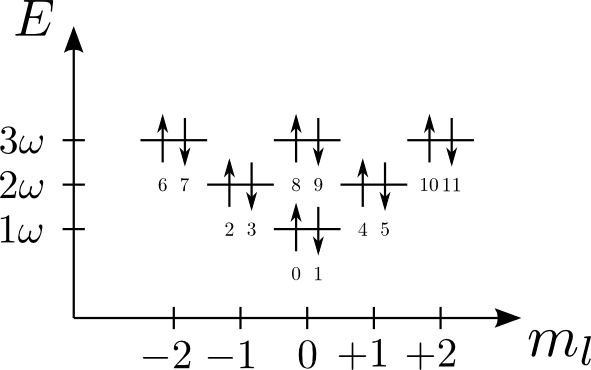
\includegraphics[scale=1.5]{../07-qDots/figs/spektrum.png}
\caption{The indexing sequence used for quantum dots, implemented in `HObasis'.}
\label{fig:qDots:qDotIndex}
\end{center}
\end{figure}



The simplest implementation of a system can be as simple as shown in listing~\ref{lst:qDots:SpecificSystem1}, explained as follows;
\begin{itemize}
\item[Line 1:~] We declare a new subclass of `System'. This provides storage objects for both one-particle and two-particle interactions as well as \textit{getter} methods to these storage objects.
\item[Line 4:~] The most important part in the constructor is to create a sensible `Basis', here using the default basis with 2 electrons (hole-states) and 10 virtual (particle-)states. `fillMatrixElements()' is a method defined in `System' that will fill all storage objects with values from `f\_elem' and `v\_elem' using the size of our basis, stored in `basis'.
\item[Line 12:] `f\_elem' calculates the normal-ordered one-particle element $f_{pq}$, defined in eq.~\eqref{eq:manybody:f_elem}. 
\item[Line 21:] `v\_elem' defines a way to calculate the antisymmetrized two-particle element $\langle pq || rs \rangle $, defined in eq.~\eqref{eq:manybody:v_elem}.
\end{itemize}
\begin{lstlisting}[float,label={lst:qDots:SpecificSystem1},caption={Example on how to implement a specific system by extending the `System' super class.}]
class SpecificSystem1 : public System
{
public:
	SpecificSystem1()
	{
		std::size_t n_elec = 2;
		std::size_t n_virtual = 10;
		this->basis = new Basis(n_elec, n_virtual);
		fillMatrixElements();
	}
	
	virtual double f_elem(std::size_t p, std::size_t q) const
	{
		double h0_pq = //Some expression for h0
		double u_pq = 0;
		for(size_t i = 0; i < basis->get_nH(); i++)
			u_pq += v_elem(p, i, q, i);
		return h0_pq + u_pq;
	}
	
	virtual double v_elem(std::size_t p, std::size_t q, std::size_t r, std::size_t s) const
	{
		double v_pqrs = //Some expression for <pq||rs>
		return v_pqrs;
	}
};
\end{lstlisting}
One should in particular note that these overridden functions are declared virtual. In this way it is possible to create solvers taking a pointer to any `System', still invoking the methods from the correct subclass. 
Listing~\ref{lst:qDots:virtual_p1} illustrates this, using a `System' pointer to access one single-particle element from a specific subclass.
\begin{lstlisting}[float,label={lst:qDots:virtual_p1},caption={A subclass has implemented the function `f\_elem()' returning the element $f_{02}$. The `System' base class has this method declared virtual, resulting in invoking the subclass implementation even when using a super-class pointer.},name={lst:qDots:virtual}]
//anySystem can point to any system,
System * anySystem = new SpecificSystem();
//and still get an element from the correct subclass
double f_02 = anySystem->f_elem(0,2);
\end{lstlisting}

Another way of accessing the same element is to get the storage matrices directly. There are three storage containers for $f_{pq}$; `f\_hh' contains only the part where both $p$ and $q$ are hole-states, `f\_ph' contains only the part where $p$ is a particle-state and $q$ is a hole-state, and `f\_pp' contains only the part with both $p$ and $q$ being particle states.
As an example we recall `SpecificSystem1' having $n_h = 2$ and $n_p = 10$.
If one would like to extract $f_{02}$ one must note that $2$ is the first particle-state, and $0$ is the first hole-state. 
Being symmetric we see how this can be found in the `f\_ph' part,
\begin{equation}
f_{02} = f_{20} = f^{ph}_{00},
\end{equation}
as implemented in listing~\ref{lst:qDots:virtual_p2}.
\begin{lstlisting}[float,label={lst:qDots:virtual_p2},caption={Continuing listing~\ref{lst:qDots:virtual_p1} extracting the same element, $f_{02}$, now through the raw storage matrix for $f$. This example assumes two occupied (hole) states, thus making index $2$ the first ($0$) particle state. With symmetric interaction matrices we expect $f_{ph} = f_{hp}^T$.},name={lst:qDots:virtual}]
mat const * f_hp;
//Get element from raw storage matrix.
f_hp = trans(anySystem->get_f_ph());
f_02 = (*f_ph)(0,0);
\end{lstlisting}

\paragraph*{}
Although the implementation in listing~\ref{lst:qDots:SpecificSystem1} is very simple, counting only 26 lines of code, this would work perfectly for small systems.
For larger systems one would encounter two problems.
Invoking `fillMatrixElements()' will force calculation of all elements every time a `SpecificSystem1' is constructed, a problem discussed later in section~\ref{sec:qDots:TPfile}.
The other problem is that the dimensionality of two-particle interactions scales as the number of virtual states to the fourth power, possibly solved by exploiting symmetries in our Hamiltonian to avoid store a tremendous amount of zero-filled elements.


\subsection{Symmetries in the Hamiltonian}
Two-particle matrix elements $\langle pq||rs \rangle$ can be interpreted as the probability for two particles making a transition from states $r$ and $s$ into $p$ and $q$.
If our Hamiltonian preserves some quantum numbers, this transition is not possible, and thus zero, whenever $pq$ does not preserve the numbers from $rs$.
In the case of quantum dots, we encounter a Hamiltonian that is spherical symmetric, and not spin dependent.
This results in preserving both the angular-momentum quantum number $m (\equiv m_l)$ as well as spin $m_s$.
Defining $M =m^p + m^q, M' = m^r + m^s$ and $M_s = m_s^p + m_s^q, M'_s = m_s^r + m_s^s$, the following holds true,
\begin{equation}
\langle n^p m^p m_s^p; n^q m^q m_s^q || n^r m^r m_s^r; n^s m^s m_s^s \rangle
= 
0
\hspace{3mm}\textrm{if}\hspace{3mm}
M \neq M'
\hspace{3mm}\textrm{or}\hspace{3mm}
M_s \neq M'_s .
\end{equation}

More generally we define a mapping
$(p,q) \leftrightarrow (\lambda,\pi)$
where $\lambda$ is a transition channel, consisting of a specific set of preserved quantum numbers, and a configuration $\pi$ for each possible combination of $(p,q)$ within that channel, such that 
\begin{equation}
\langle \lambda \pi || \lambda' \pi' \rangle = 0
\hspace{3mm}\textrm{if}\hspace{3mm}
\lambda \neq \lambda' .
\end{equation}
This re-indexing allows us to store the interaction elements as a block-diagonal matrix, one block  for each channel $\lambda$, stored as a matrix $\langle \pi || \pi' \rangle_{\lambda}$.
We further split the interaction matrices whether their indices are above ($a,b,c,d$) or below ($i,j,k,l$) the Fermi-level, resulting in six matrices,
\begin{equation}
\label{eq:qDots:split6tpelem}
\begin{split}
\langle ij||kl \rangle& \\
\langle aj||kl \rangle& = -\langle ja||kl \rangle = \langle kl||aj \rangle = -\langle kl||ja \rangle \\
\langle ab||kl \rangle& = \langle kl||ab \rangle \\
\langle aj||cl \rangle& = -\langle aj||lc \rangle = \langle ja||lc \rangle = -\langle ja||cl \rangle\\
\langle ab||cl \rangle& = -\langle ab||lc \rangle = \langle cl||ab \rangle = \langle lc||ab \rangle \\
\langle ab||cd \rangle&  .\\
\end{split}
\end{equation}
Splitting configurations into configurations for hole-hole states, particle-hole states and particle-particle states, yielding the mappings
\begin{equation}
\begin{split}
(i,j) &\leftrightarrow (\lambda, \mu), \\
(a,j) &\leftrightarrow (\lambda, \nu), \\
(a,b) &\leftrightarrow (\lambda, \xi),
\end{split}
\end{equation}
we can use a storage scheme in `System' objects splitting interactions into six parts similarly to eq.~\eqref{eq:qDots:split6tpelem}, exploiting the sparseness to store block-diagonal parts of the six matrices only, 
\begin{equation}
\begin{split}
\langle \mu || \mu' \rangle_{\lambda},& \hspace{5mm}
\langle \nu || \mu \rangle_{\lambda}, \\
\langle \xi || \mu \rangle_{\lambda},& \hspace{5mm}
\langle \nu || \nu \rangle_{\lambda}, \\ 
\langle \xi || \nu \rangle_{\lambda},& \hspace{5mm}
\langle \xi || \xi \rangle_{\lambda} .
\end{split}
\end{equation}

Mappings from states into channels and configurations are managed by the `Basis' class, and one could access these mappings through the eight methods  in listing~\ref{lst:qDots:accessMappings}.
\begin{lstlisting}[float,label={lst:qDots:accessMappings},caption={There are eight different mappings possible to access through the basis object.}]
//Mappings from (pq,lm,dl,de) into lmd and (pi,mu,nu,xi)
get_map_lmdPI_pq();
get_map_lmdMU_lm();
get_map_lmdNU_dl();
get_map_lmdXI_de();

//Reverse mappings 
get_map_pq_lmdPI();
get_map_lm_lmdMU();
get_map_dl_lmdNU();
get_map_de_lmdXI();
\end{lstlisting}
In this context two general states are encoded to one index, $\mathrm{I}$, i.e.
\begin{equation}
\begin{split}
\mathrm{I}(pq) &= p + q \cdot (n_h + n_p) \\
\mathrm{I}(lm) &= l + m \cdot n_h \\
\mathrm{I}(dl) &= d + l \cdot n_p \\
\mathrm{I}(de) &= d + e \cdot n_p,
\end{split}
\end{equation}
where $n_h$ is the number of hole-states, and $n_p$ the number of particle-states.
Returning to our example of `SpecificSystem1' we have $n_h=2, n_p=10$, and trying to access the matrix element $\langle 20||20 \rangle$ we can use either the procedure from listing~\ref{lst:qDots:mapForward}, extracting the raw matrices, or use the `v\_elem' method as in listing~\ref{lst:qDots:mapBackward}.
\begin{lstlisting}[float,label={lst:qDots:mapForward},caption={We try to access the element $\langle 20||20 \rangle$ by mapping the $|20\rangle$ particle-hole state into a channel and a configuration, $|\nu\rangle_{\lambda}$.},name={lst:qDots:map}]
//Create a specific system
SpecificSystem1 sys;

//Get informations about its basis
Basis const * basis = sys.get_basis();
int nH = basis->get_nH(); //hole-states
int nP = basis->get_nP(); //particle-states

//(d,l) = (2,0) is a particle hole configuration.
int d = 2 - nH;
int l = 0;
int dl = d + l * nH;

//Map into a channel and a configuration.
umat const * map = basis->get_map_dl_lmdNU();
int lmd = (*map)(0,dl); //first row contains lambda values.
int nu = (*map)(1,dl); //second row contains configurations.

//Retreive element;
vector<mat> const * phph = sys->get_v_phph();
double elem_20_20 = phph->at(lmd)(nu,nu);
\end{lstlisting}
\begin{lstlisting}[float,label={lst:qDots:mapBackward},caption={Continuing listing~\ref{lst:qDots:mapForward}, accessing the same element again, $\langle \nu || \nu \rangle_{\lambda} = \langle 20||20 \rangle$, now using the reverse mapping, $|\nu\rangle_{\lambda} \rightarrow |20\rangle$.},name={lst:qDots:map}]
//Map back to two states d,l
vector<uvec> const * mapback = basis->get_map_lmdNU_dl();
dl = mapback->at(lmd)(nu);
d = dl % nP + nH;
l = dl / nP;

//this should return the same element
elem_20_20 = sys->v_elem(d,l,d,l);
\end{lstlisting}

\paragraph*{}
The default `Basis' base class will assume only one transition channel, resulting in storing all interaction elements.
For quantum dots we have $M,M_s \leftrightarrow \lambda$, implemented in `HOBasis'.
As an example of the reduced dimensionality, we consider a harmonic oscillator basis with 20 electrons and 400 virtual states.
The largest matrix would be $\langle ab||de \rangle$ with a dimensionality of $400^4$, resulting in $\sim 200$GB of storage!
Exploiting the symmetries and employing an `HOBasis' instead reduces this to $\sim 1.75$GB.
Readers are encouraged to read through this implementation as an example of subclassing `Basis'.



\subsection{Reading elements from file}
\label{sec:qDots:TPfile}
Another time-consuming part is to calculate the matrix elements, which could be performed once and later read from file. 
To create a system read from file, it is convenient to create a subclass of `TPfile', and we take the actual implementation for circular quantum-dots `CQDot' as an example.
There are three methods, shown in listing~\ref{lst:qDots:CQDotMinimumHeader}, which must be overloaded.
\begin{lstlisting}[float,label={lst:qDots:CQDotMinimumHeader},caption={The three most important parts a subclass of `TPfile' would need. The actual implementation of `CQDot' includes some extra methods and private variables.}]
class CQDot : public TPfile
{
public:
  //#1- Constructor
  CQDot(int filledR, int shellsR, double omega = 1.0);
  
  //#2- Calculation of one-particle element f_{pq}
  virtual double f_elem(std::size_t p, std::size_t q) const
  {
    //Part arising from normal ordering
    double u_pq = 0.0;
    for (int i = 0; i < basis->get_nH(); i++)
      u_pq += v_elem(p, i, q, i);
    
	//Part from h0
    ivec3 p_NMMs = basis->stateMap(p);
    int n = pNMMs(0);
    int m = pNMMs(1);
    double h0 = omega * (2 * n + abs(m) + 1);

	//h0 is diagonal
	if (p == q)
      return h0 + u_pq;     
    else
      return u_pq;
  }

protected:
  //#3- A recipe on how to decode tp-element file.
  virtual size_t interp_qNum(char* qNumbers) const;
};
\end{lstlisting}
The constructor takes three arguments; the number of filled shells, the total number of shells and the frequency, $\omega$.

Looking at the constructor's implementation, listing~\ref{lst:qDots:constructor}, we remark how `fillMatrixElements' is no longer called to fill both one- and two-particle elements. 
Instead we read elements $\langle pq||rs \rangle$ from file using `readFileName', and later calculate $f_{pq}$ by invoking 'fillFmatrix'. Both these methods are public, and can therefore be invoked from the main program.
We create a basis, `HOBasis', store the frequency in a private variable, and create a reverse statemap to be used later when reading a file.
This reverse statemap assigns a unique key (unsigned int), constructed from the three quantum numbers, to each state, and it is later possible to get the single index for any state by constructing the same key.
\begin{lstlisting}[float,label={lst:qDots:constructor},caption={Constructor for CQDot.}]
CQDot::CQDot(int filledR, int totalR, double omega)
{
    //Initialize basis and frequency
    basis = new HOBasis(filledR, totalR);
    this->omega = omega;

    //Creating reversed state map, needed when reading file
    int ntot = basis->get_nH() + basis->get_nP();
    for (int state = 0; state < ntot; state++)
    {
    	//Extract quantum numbers n,m,m_s
        ivec3 nmms = basis->stateMap(state);
        unsigned int n = nmms(0);
        int m = nmms(1);
        unsigned int ms = nmms(2);
        
        //Each state has a unique key.
        unsigned int key = n + (m + (ms + hMaxM) * maxM) * maxM;
        revMap[key] = state;
    }
}
\end{lstlisting}

One-particle elements are still calculated through `f\_elem()', implementing the single-particle energies from eq.~\eqref{eq:qDots:spEnergies} combined with a normal-ordered part as in eq.~\eqref{eq:manybody:f_elem}, viz
\begin{equation}
f_{pq} = \delta_{pq} \left(1 + |m| + 2n \right) \omega   + \sum_{i} \langle pi||qi \rangle .
\end{equation}
Depending on $\langle pi||qi \rangle$, one-particle elements are required to be filled first after two-particle elements are read from file, by invoking `fillFmatrix'.

Two-particle elements are read through the method `readFileName', redirecting to `readFileStream' in listing~\ref{lst:qDots:readFileStream}.
The file-reading itself is already implemented in the base class, and we expect elements on file to be for $\omega=1$, such that we need only to scale $\omega$ after reading.
Invoking `TPfile::readFileStream' will force the base-class implementation to be run even though these functions are declared as virtual.
The last steps are to scale elements\footnote{Only standard interaction can be scaled by $\sqrt{\omega}$, forcing us to create another file-reading routine `readEffFileStream' (and `readEffFileName') for effective interactions.} by $\sqrt{\omega}$ and fill the single-particle elements.
\begin{lstlisting}[float,label={lst:qDots:readFileStream},caption={How to read tp-elements for CQDot.}]
void CQDot::readFileStream(std::ifstream &file)
{
    //First read file as done in super class.
    TPfile::readFileStream(file);
    //Then scale by sqrt(omega)
    size_t dimLMD = basis->dim_lmd_2p();
    for (size_t lmd = 0; lmd < dimLMD; lmd++)
    {
        v_hhhh.at(lmd) = sqrt(omega) * v_hhhh.at(lmd);
        v_phhh.at(lmd) = sqrt(omega) * v_phhh.at(lmd);
        v_pphh.at(lmd) = sqrt(omega) * v_pphh.at(lmd);
        v_phph.at(lmd) = sqrt(omega) * v_phph.at(lmd);
        v_ppph.at(lmd) = sqrt(omega) * v_ppph.at(lmd);
        v_pppp.at(lmd) = sqrt(omega) * v_pppp.at(lmd);
    }
    //Fill one-particle elements.
    fillFmatrix();
}
\end{lstlisting}

In order to successfully read elements from file the base class needs some information about the file structure, found through the sub-class implementation of `interp\_qNum'.
A basic file format is expected to be binary with the content,
\begin{verbatim}
p q r s <pq||rs> p' q' r' s' <p'q'||r's'> ... ,
\end{verbatim}
p is a number of bytes, $n_{b}$, needed to specify the state $p$, q is $n_b$ bytes necessary to specify $q$, and so on until the element itself $\langle pq||rs \rangle$ stored as a `double'. 
The implementation for quantum dots may serve as an example.
Here $n,m$ and $m_s$ are coded as an unsigned short, a short and a char. 
This is repeated for all four states an element consists of, followed by the element itself,
\begin{equation}
\underbrace{
\overbrace{n^p}^\text{ushort (2B)} 
\overbrace{m^p}^\text{short (2B)}
\overbrace{m_s^p}^\text{char (1B)}
}_\text{numBytes (5B)}
\underbrace{n^q m^q m_s^q}_\text{(5B)}
\underbrace{n^r\hspace{2mm}m^r\hspace{2mm}m_s^r\hspace{2mm}}_\text{(5B)}
\underbrace{n^s\hspace{2mm}m^s\hspace{2mm}m_s^s\hspace{2mm}}_\text{(5B)}
\underbrace{\langle pq||rs \rangle}_\text{double (8B)} .
\end{equation}
On most platforms this would require 5 bytes for each state, and 8 bytes for the element, as noted in parentheses.
In order to know how many bytes are expected to describe each state, `interp\_qNum(NULL)' is queried.
Once those bytes are read from file they are sent to the same method as a char array, and expected return is a single integer indexing the correct state.
For `CQDot', implementation in listing~\ref{lst:qDots:interp_qNum}, the char array is split into an unsigned short, short and a char, and correct state is found using the reverse state map that was initialized in the constructor.
\begin{lstlisting}[float,label={lst:qDots:interp_qNum},caption={Implementation of `interp\_qNum' in `CQDot'.}]
size_t CQDot::interp_qNum(char* qNumbers) const
{
    //Quantum numbers n, m, m_s read from file.
    unsigned short n;
    short m;
    char ms;
    
    //Single indexed state
    size_t state;

    //The number of bytes for each state
    if (qNumbers == NULL)
        return sizeof (n) + sizeof (m) + sizeof (ms);

    //Split qNumbers!
    size_t siz_n = sizeof (n);
    memcpy(&n, qNumbers, siz_n);
    size_t siz_m = sizeof (m);
    memcpy(&m, qNumbers + siz_n, siz_m);
    size_t siz_ms = sizeof (ms);
    memcpy(&ms, qNumbers + siz_n + siz_m, siz_ms);

    //Encode spin
    if (ms == -1) 
        ms = 1; //down
    else if (ms == +1)
        ms = 0; //up
    
    //unique key for any state
    unsigned int key = n + (m + (ms + hMaxM) * maxM) * maxM;
    //revMap is a std::map filled in the constructor
    const map<unsigned int, unsigned int>::const_iterator found = revMap.find(key);
    
    if (found == revMap.end())
        state = maxM;  //A state outside the current basis
    else
        state = found->second; //State found in current basis

    return state;
}
\end{lstlisting}


A complete file can be read from file in a simple way, as listing~\ref{lst:qDots:readElem} shows, reading one element at a time, adding a  simple loop to read all elements in a file.
\begin{lstlisting}[float,label={lst:qDots:readElem},caption={How to read two-particle elements from file.}]
void TPfile::readFileStream(std::ifstream &file)
{
  //Number of bytes to read for each state.
  size_t qNumWidth = interp_qNum(NULL);
  char * qNumP = new char[qNumWidth];
  char * qNumQ = new char[qNumWidth];
  char * qNumR = new char[qNumWidth];
  char * qNumS = new char[qNumWidth];

  //Allocate memory for tp-elements.
  //......

  while (true)
  {
    //Read one `line' from file
    double element = 0;
    file.read(qNumP, sizeof (char) * qNumWidth);
    file.read(qNumQ, sizeof (char) * qNumWidth);
    file.read(qNumR, sizeof (char) * qNumWidth);
    file.read(qNumS, sizeof (char) * qNumWidth);
    file.read((char*) &element, sizeof (double));
    if (file.eof())
      break;  //End of file?

	//Find the index
    size_t p = interp_qNum(qNumP);
    size_t q = interp_qNum(qNumQ);
    size_t r = interp_qNum(qNumR);
    size_t s = interp_qNum(qNumS);

    //Store all antisymmetric possibilities 
    storePQRS(p, q, r, s, element);
    storePQRS(p, q, s, r, -element);
    storePQRS(q, p, s, r, element);
    storePQRS(q, p, r, s, -element);
  }

  //Free the four char arrays
  //......
}
\end{lstlisting}
The functionality to read files is already implemented in the two methods `readFileName' and `readFileStream'.






\section{Other systems}
Other systems may equally well be implemented, and should be compatible with the different solvers as long as they extend the `System' and `Basis' base classes properly.
As an example we have implemented a simple class, `Atoms', outlined in listings~\ref{lst:qDots:atoms_p1} and~\ref{lst:qDots:atoms_p2}, that include the 8 lowest-lying s-states\footnote{Atomic orbitals are distinguished by their angular momentum quantum number $l$. If $l=0$ the state is said to be \textbf{s}harp, an `s-state'. Continuing, for $l=1,2,3$, we have \textbf{p}rinciple, \textbf{d}iffuse and \textbf{f}undamental.} of atomic orbitals.
The single-particle energies are found in the Bohr-model to be
\begin{equation}
E_n = \frac{Z^2}{2n^2}, \hspace{4mm}\textrm{(in atomic units)},
\end{equation}
and the two-particle correlation elements are found by integrating the Coloumb energies for the atomic orbitals, either calculated analytically by hand or computer algebra software, or by numerical integration.
\begin{lstlisting}[float,label={lst:qDots:atoms_p1},caption={Simple implementation for the first sharp atomic orbitals. Continued in listing~\ref{lst:qDots:atoms_p2}.},name={lst:qDots:atoms}]
class Atoms : public System
{
public:
  /** numElec is 2 for helium, 4 for beryllium */
  Atoms(int numElec = 2)
  {
    //Charge from nucleus defaults to number of electrons
    Z = numElec;
    //There are only 8 states implemented
    basis = new Basis(numElec, 8 - numElec);
    //Fill matrices
    fillMatrixElements();
  }

  virtual double f_elem(std::size_t p, std::size_t q) const
  {
    //Normal-ordered part
    double u_pq = 0;
    for (int i = 0; i < basis->get_nH(); i++)
        u_pq += v_elem(p, i, q, i);
	//single-particle energies
    int n = p / 2 + 1;	 //n is the energy level
	double h0 = -pow((double) Z, 2) / (2 * n * n);
	//h0 is diagonal
    if (p == q)
      return h0 + u_pq;
    else
      return u_pq;
  }
\end{lstlisting}
\begin{lstlisting}[float,label={lst:qDots:atoms_p2},caption={Continuation of listing~\ref{lst:qDots:atoms_p1}.},name={lst:qDots:atoms}]
  virtual double v_elem(
    std::size_t p, std::size_t q,
    std::size_t r, std::size_t s) const
  {
    //Get spin of particles
    bool pUP = p % 2 == 0;
	//... same for q,r and s ...

    //Map p,q,r,s to n quantum number
    int n_p = p / 2 + 1;
    //... same for q,r and s ...

    //First term of element
    double term1 = 0;
    if (pUP == rUP && qUP == sUP)
        term1 = spatial_integral(n_p, n_q, n_r, n_s);
    //Second term
    double term2 = 0;
    if (pUP == sUP && qUP == rUP)
        term2 = spatial_integral(n_p, n_q, n_s, n_r);
	
    return term1 - term2;
  }

  /** The spatial integral of correlation energies can be
  /*  found analytically (and tabulated) using Mathematica
  /*  or Maple. Also possible to find through numerical
  /*  integration. (four lowest lying orbitals only) */
  double spatial_integral(int n_p, int n_q, int n_r, int n_s) const;
            
private:
  /** The total charge in the nucleus */
  double Z ;
};
\end{lstlisting}


\paragraph{}
If we were to extend the Harmonic Oscillator basis to three dimension, we would have a basis often used in nuclear physics. 
In that case, one would need one additional quantum numbers for the orbitals, as well as quantum numbers describing different types of particles.
Although not done in this thesis, it should, in the author's opinion, not be too complicated.
However, nuclear calculations often require a larger dimensionality, and further simplifications, known as jj scheme, exist.

\paragraph{}
The hierarchy of implemented classes is shown in fig.~\ref{fig:qDots:classTree}, where `CQDot', `TPfile' and `Atoms' are already discussed.
`HFsys' is used to obtain a Hartree-Fock transformed basis, as discussed in the next chapter, copying the basis object and transforming the elements from any arbitrary system.
\begin{figure}
\begin{center}
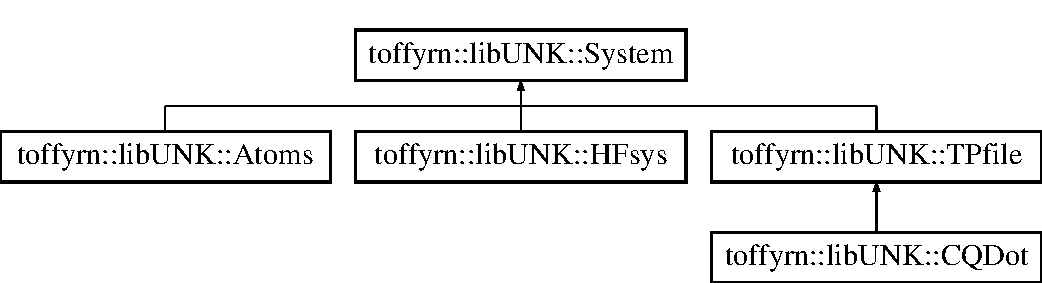
\includegraphics[scale=0.8]{../07-qDots/figs/classTree.pdf}
\caption{Hierarchy of implemented `System' subclasses. `CQDot' is our implementation for circular quantum dots, gaining simplicity by extending the file-reading methods from `TPfile'. `Atoms' defines a simple system including a basis of a few atomic orbitals. The last class, `HFsys', can obtain a Hartree-Fock transformed basis from any other system, as discussed in the next chapter.}
\label{fig:qDots:classTree}
\end{center}
\end{figure}





\chapter{Coupled cluster theory}
Coupled cluster~(CC) is an \textit{ab initio} method for solving the quantum mechanical many-body problem.
It was first introduced by Coester and Kümmel during the 1950s \cite{NucPhys.7.421,NucPhys.17.477},
originally developed for problems in nuclear physics, but later reformulated for systems of electrons by \v{C}i\v{z}ek in 1966 \cite{ChemPhys.45.4256}.
Even though it is somewhat computationally expensive it is one of the most popular post-Hartree-Fock methods today, due to good accuracy as well as important features like size-consistency and size-extensivity.

\section{The exponential ansatz}
The foundation for most many-body methods is to express the correct wave function by an expansion in a set of basis functions. 
One example is the Hartree-Fock~(HF) method which employs a unitary transformation of the single-particle wave functions, 
\begin{equation}
|\lambda \rangle = \sum_{\psi} C_{\lambda \psi} |\psi \rangle ,
\end{equation}
and approximates the ground state with a reference Slater determinant built up by these transformed wave functions.
Another example is configuration interaction~(CI) where the reference determinant is set to a linear expansion of determinants, including the initial reference determinant, 1p-1h excitations, 2p-2h excitations and so on, i.e.
\begin{equation}
|\Psi_{0}^{CI} \rangle = C_0 |\Phi_0 \rangle + \sum_{ia} C_i^a |\Phi_i^a\rangle + \sum_{ijab} C_{ij}^{ab} |\Phi_{ij}^{ab} \rangle + \cdots \hspace{2mm}.
\end{equation}
In all these methods one needs to solve a set of coupled equations to find these coefficients.

\paragraph*{}
The Coupled cluster method also expands the exact solution in a set of Slater determinants, but employs a non-linear expansion through the exponential ansatz,
\begin{equation}
\label{eq:CC:expon}
|\Psi_0^{CC} \rangle = e^{\hat{T}} |\Phi_0 \rangle ,
\end{equation}
where $\hat{T}$ is the cluster operator including \textit{all} possible excitations on the reference determinant.
Sorting excitations by the number of excited electrons, we may generally express this general cluster operator as a sum of a 1p-1h operator, a 2p-2h operator, and so on,
\begin{equation}
\hat{T} = \hat{T_1} + \hat{T_2} + \hat{T_3} + \cdots \hspace{2mm}.
\end{equation}
In the form of second-quantized operators the 1p-1h cluster operator is defined as
\begin{equation}
\hat{T}_1 = \sum_{ia} t_i^a \hat{a}^{\dagger} \hat{i},
\end{equation}
the 2p-2h cluster operator as
\begin{equation}
\hat{T}_2 = \frac{1}{4} \sum_{ijab} t_{ij}^{ab} \hat{a}^{\dagger} \hat{b}^{\dagger} \hat{j} \hat{i},
\end{equation}
continuing up to 
\begin{equation}
\hat{T}_n = \left( \frac{1}{n!}\right)^2 \sum_{ij\cdots ab\cdots} t_{ij\cdots}^{ab\cdots} \hat{a}^{\dagger} \hat{b}^{\dagger} \cdots \hat{j} \hat{i} .
\end{equation}
As long as we have a complete single-particle basis and include all possible excitations up to $n$p-$n$h in a system with $n$ particles, we should find the exact solution for both CI, $|\Psi_0^{CI}\rangle$, and CC, $|\Psi_0^{CC}\rangle$.

\paragraph*{}
It is of course not doable to find the exact solution in practice.
A complete single-particle basis would typically mean an infinite set of basis functions.
In addition we would need all excitations up to $n$p-$n$h determinants, yielding a huge amount of determinants. 
This is why all methods need a computational cut-off.
Two types of truncations are used.
First we truncate the number of single-particle basis functions, throwing away the ones with the highest energies, which makes sense since our interest is in the ground-state energy.
Second we truncate the number of excitations we include, giving rise to different types of the coupled cluster method.
Including the singly excited cluster operator the method is labeled by S, for `single', and including the doubly excited cluster operator the label D is added, for `double'.
This thesis has an emphasis on CCSD -- `Coupled Cluster Singles and Doubles'.

\section{Derivation of the CCSD-equations}
It is quite tedious work to derive the CCSD equations by hand, but we will present a diagrammatic approach in this section along with some explaining comments where needed. 

\paragraph{}
We aim to find the solution to the time-independent energy eigenvalue equation,
\begin{equation}
\hat{H} |\Psi_0 \rangle = E_0 |\Psi_0 \rangle
\cong
\hat{H} e^{\hat{T}} |\Phi_0 \rangle = E_0 e^{\hat{T}} |\Phi_0 \rangle ,
\end{equation}
assuming $|\Psi_0\rangle$ can be approximated by the exponential ansatz~\eqref{eq:CC:expon}. 
It is useful to project $\langle \Phi_0 | e^{-\hat{T}}$ onto the eigenvalue equation to get an explicit expression for the energy,
\begin{equation}
\langle \Phi_0 | e^{-\hat{T}} \hat{H} e^{\hat{T}} |\Phi_0 \rangle 
=
\langle \Phi_0 | e^{-\hat{T}} E_0 e^{\hat{T}} |\Phi_0 \rangle
= E_0 .
\end{equation}
We may also project this onto an excited determinant, assuming orthonormal basis functions, and exploit the fact that excited states should be orthogonal to the reference determinant,
\begin{equation}
\langle \Phi_{exc.} | e^{-\hat{T}} \hat{H} e^{\hat{T}} |\Phi_0 \rangle 
=
\langle \Phi_{exc.} | e^{-\hat{T}} E_0 e^{\hat{T}} |\Phi_0 \rangle
=
E_0 \langle \Phi_{exc.} | \hat{1} |\Phi_0 \rangle
= 0 .
\end{equation}
Further simplification is found if we use the normal-ordered Hamiltonian~\eqref{eq:manybody:normhamil}, leading to
\begin{equation}
\begin{split}
\langle \Phi_0 | e^{-\hat{T}} \hat{H}_N e^{\hat{T}} |\Phi_0 \rangle 
=&
\langle \Phi_0 | e^{-\hat{T}} \hat{H} e^{\hat{T}} |\Phi_0 \rangle - E_{ref}
=
E_0 - E_{ref} \\
\langle \Phi_{exc.} | e^{-\hat{T}} \hat{H}_N e^{\hat{T}} |\Phi_0 \rangle 
=&
\langle \Phi_{exc.} | e^{-\hat{T}} (E_0 - E_{ref}) e^{\hat{T}} |\Phi_0 \rangle
=
0 .
\end{split}
\end{equation}


\paragraph*{}
In the following derivation $i,j,k$ and $a,b,c$ will refer to indices in the bra state, whereas 
$d,e,...$ and $l,m,...$ are free indices to be summed over, still restricting $a,b,c,d,e,...$ to particle states and $i,j,k,l,m,...$ to hole states.
There are three equations that, in the case of singles and doubles, needs to be solved,
\begin{equation}
\begin{split}
\langle \Phi_0 | \bar{H} | \Phi_0 \rangle &= E_0  - E_{ref} \\
\langle \Phi_{i}^a | \bar{H} | \Phi_0 \rangle &= 0 \\
\langle \Phi_{ij}^{ab} | \bar{H} | \Phi_0 \rangle &= 0 .
\end{split}
\end{equation}
The first gives us an explicit form for the energy, whereas the other two will determine the amplitudes in the cluster operators.
The similarity transformed Hamiltonian, denoted $\bar{H}$, can be evaluated as a series of commutators, using the Baker-Campbell-Hausdorff formula,
\begin{equation}
\label{eq:CC:BCH}
\bar{H} \equiv e^{-\hat{T}} \hat{H}_N e^{\hat{T}}
=
\hat{H}_N + \left[\hat{H}_N, \hat{T} \right]
+
\frac{1}{2!} \left[\left[\hat{H}_N, \hat{T}\right], \hat{T}\right]
+
\frac{1}{3!} \left[\left[\left[\hat{H}_N, \hat{T} \right], \hat{T}\right], \hat{T}\right] + \cdots\hspace{2mm}.
\end{equation}

Let $\hat{A}$ and $\hat{B}$ be two normal-ordered strings of operators containing an even number of creation and annihilation operators. Using Wick's generalized theorem, their commutator would be
\begin{equation}
\left[ \hat{A}, \hat{B} \right]
=
\left\lbrace \hat{A}\hat{B} \right\rbrace - \left\lbrace \hat{B}\hat{A} \right\rbrace
+
\left\lbrace
\contraction[1ex]{}{\hat{A}}{}{\hat{B}}
\hat{A}\hat{B} \right\rbrace
-
\left\lbrace
\contraction[1ex]{}{\hat{B}}{}{\hat{A}}
\hat{B}\hat{A} \right\rbrace ,
\end{equation}
where the two uncontracted terms are the same, and we thus end up with
\begin{equation}
\left[ \hat{A}, \hat{B} \right]
=
\left\lbrace
\contraction[1ex]{}{\hat{A}}{}{\hat{B}}
\hat{A}\hat{B} \right\rbrace
-
\left\lbrace
\contraction[1ex]{}{\hat{B}}{}{\hat{A}}
\hat{B}\hat{A} \right\rbrace .
\end{equation}
We observe that the cluster operators are already normal-ordered, and also note how no contractions between a cluster operator on the left and any other operator on the right can be non-zero.
This is because the $\hat{T}$ operator contains $\hat{a}^{\dagger} \hat{b}^{\dagger} \cdots \hat{j}\hat{i}$, none of which can lead to any non-zero contraction from~\eqref{eq:manybody:referencecontractions}.
The cluster operators thus commute, yielding
\begin{equation}
\left[ \hat{T}_n, \hat{T}_m \right]
=
\left\lbrace
\contraction[1ex]{}{\hat{T}_n}{}{\hat{T}_m}
\hat{T}_n \hat{T}_m \right\rbrace
-
\left\lbrace
\contraction[1ex]{}{\hat{T}_m}{}{\hat{T}_n}
\hat{T}_m \hat{T}_n \right\rbrace
=
0 .
\end{equation}

We may also explore how the cluster operators commute with the Hamiltonian.
Once again terms with $\hat{T}_n$ on the left are zero, and we are left with
\begin{equation}
\left[ \hat{H}_N, \hat{T}_n \right]
=
\left\lbrace
\contraction[1ex]{}{\hat{H}_N}{}{\hat{T}_n}
\hat{H}_N \hat{T}_n \right\rbrace
-
\left\lbrace
\contraction[1ex]{}{\hat{T}_n}{}{\hat{H}_N}
\hat{T}_n \hat{H}_N \right\rbrace
=
\left\lbrace
\contraction[1ex]{}{\hat{H}}{}{\hat{T}_n}
\hat{H}_N \hat{T}_n \right\rbrace .
\end{equation}
Applying this recursively to write out~\eqref{eq:CC:BCH} it becomes clear that all surviving terms have $\hat{H}_N$ to the left, and all the cluster operators should have at least one contraction each to the Hamiltonian.
These terms are referred to as connected terms (subscript $\mathit{C}$), and because the electronic Hamiltonian includes no more than four operators it would not be possible to find connected terms with more than four cluster operators, posing a natural truncation to $\bar{H}$, 
\begin{equation}
\label{eq:CC:barhconn}
\bar{H} 
= \left(\hat{H}_N e^{\hat{T}} \right)_{\mathit{C}}
= \hat{H}_N 
+ \left( \hat{H}_N \hat{T} \right)_{\mathit{C}}
+\frac{1}{2} \left( \hat{H}_N \hat{T}^2 \right)_{\mathit{C}}
+\frac{1}{3!} \left( \hat{H}_N \hat{T}^3 \right)_{\mathit{C}}
+\frac{1}{4!} \left( \hat{H}_N \hat{T}^4 \right)_{\mathit{C}} .
\end{equation}


\subsection{Diagrammatic rules}
It is now possible to write out all possible terms and evaluate them diagrammatically. 
Writing out each term as a diagram, a number of rules exists on how to interpret them, to find the correct algebraic expressions;
\begin{enumerate}
\item\label{ite:CC:sumFree} Sum over all \textit{free} indices. Free indices are not connected to the left determinant.
\item\label{ite:CC:operators} Interpret one-body operators as $\langle out |\hat{f}| in \rangle \equiv f_{out,in}$, and two-body operators as $\langle lout,rout || lin,rin \rangle$.
\item\label{ite:CC:phase} Add a phase factor of $(-1)^{l+h}$, where $l$ is the number of loops and $h$ is the number of hole lines.
\item\label{ite:CC:equLines} Multiply by a factor of $\frac{1}{2}$ for each pair of \textit{equivalent lines}.
Equivalent lines are starting and ending at the same interaction lines.
\item\label{ite:CC:equVert} Each pair of \textit{equivalent vertices} raises an additional factor of $\frac{1}{2}$.
Equivalent vertices are vertices of equal type connected to the same interaction lines with equivalent connecting lines.
\item\label{ite:CC:permut} Each external, unique pair of holes or particles not connected to the same interaction line leads to an antisymmetric permutation $\hat{P}_{l_1 l_2}$.
\item\label{ite:CC:signTable} If there are multiple ways to connect the diagrams, only one term should exist for each configuration in the Sign-Table technique.
\end{enumerate}
The different rules will be discussed in more detail where needed.

\paragraph*{}
It is possible to split up the sums in the interactions, specifying whether the indices are within the fermi level or not. For the one-body part there exist four possibilities,
\begin{equation}
\hat{F}_N 
=
\sum_{de} f_{de} \left\lbrace \hat{d}^{\dagger} \hat{e} \right\rbrace
+
\sum_{lm} f_{lm} \left\lbrace \hat{l}^{\dagger} \hat{m} \right\rbrace
+
\sum_{ld} f_{ld} \left\lbrace \hat{l}^{\dagger} \hat{d} \right\rbrace
+
\sum_{dl} f_{dl} \left\lbrace \hat{d}^{\dagger} \hat{l} \right\rbrace,
\end{equation}
diagrammatically represented as,
\begin{equation}
\begin{split}
\hat{F}_N
=
\parbox{25mm}{
    \textrm{
    \begin{fmffile}{fmf-cc-F_N-1}
        \begin{fmfgraph*}(50,50)
            %Upper and lower lines.
            \fmfstraight
            \fmfbottom{b1,b2} \fmftop{t1,t2}
            \fmf{phantom}{b1,fL,t1}
            \fmf{phantom}{t2,fR,b2}
            \fmf{dashes}{fL,fR}
            \fmfv{decor.shape=cross,decor.size=3mm}{fR}
            \fmffreeze
            %Electron lines
            \fmf{electron}{b1,fL}
            \fmf{electron}{fL,t1}
        \end{fmfgraph*}
    \end{fmffile}
    }
}
+
\parbox{25mm}{
    \textrm{
    \begin{fmffile}{fmf-cc-F_N-2}
        \begin{fmfgraph*}(50,50)
            %Upper and lower lines.
            \fmfstraight
            \fmfbottom{b1,b2} \fmftop{t1,t2}
            \fmf{phantom}{b1,fL,t1}
            \fmf{phantom}{t2,fR,b2}
            \fmf{dashes}{fL,fR}
            \fmfv{decor.shape=cross,decor.size=3mm}{fR}
            \fmffreeze
            %Electron lines
            \fmf{electron}{t1,fL}
            \fmf{electron}{fL,b1}
        \end{fmfgraph*}
    \end{fmffile}
    }
}
+
\parbox{25mm}{
    \textrm{
    \begin{fmffile}{fmf-cc-F_N-3}
        \begin{fmfgraph*}(50,50)
            %Upper and lower lines.
            \fmfstraight
            \fmfbottom{b1,b2} \fmftop{t1,t2}
            \fmf{phantom}{b1,fL,t1}
            \fmf{phantom}{t2,fR,b2}
            \fmf{phantom}{b1,bC,b2}
            \fmf{dashes}{fL,fR}
            \fmfv{decor.shape=cross,decor.size=3mm}{fR}
            \fmffreeze
            %Electron lines
            \fmf{electron}{b1,fL}
            \fmf{electron}{fL,bC}
        \end{fmfgraph*}
    \end{fmffile}
    }
}
+
\parbox{25mm}{
    \textrm{
    \begin{fmffile}{fmf-cc-F_N-4}
        \begin{fmfgraph*}(50,50)
            %Upper and lower lines.
            \fmfstraight
            \fmfbottom{b1,b2} \fmftop{t1,t2}
            \fmf{phantom}{b1,fL,t1}
            \fmf{phantom}{t2,fR,b2}
            \fmf{phantom}{t1,tC,t2}
            \fmf{dashes}{fL,fR}
            \fmfv{decor.shape=cross,decor.size=3mm}{fR}
            \fmffreeze
            %Electron lines
            \fmf{electron}{t1,fL}
            \fmf{electron}{fL,tC}
        \end{fmfgraph*}
    \end{fmffile}
    }
} .
\end{split}
\end{equation}
The first two terms have the same amount of lines at the top as in the bottom, and we say that these terms have an excitation level zero.
Such terms have no possibility to neither create nor annihilate a particle-hole pair.
If there is an incoming 2p-2h excitation in a diagram, there will also be an outgoing 2p-2h excitation.
The third term is said to have excitation level minus one.
When connected in a diagram it will destroy one particle-hole pair, transforming for example an incoming 2p-2h excitation into an outgoing 1p-1h excitation.
Following this reasoning, the last term has excitation level plus one.

Splitting the two-body operator similarly we get 
\begin{equation}
\begin{split}
\hat{V}_N
=
\parbox{30mm}{
    \textrm{
    \begin{fmffile}{fmf-cc-V_N-1}
        \begin{fmfgraph*}(50,50)
            %Upper and lower lines.
            \fmfstraight
            \fmfbottom{b1,b2,b3,b4} \fmftop{t1,t2,t3,t4}
			\fmf{phantom}{t1,vL,b2}
			\fmf{phantom}{t3,vR,b4}
            \fmffreeze
            \fmf{dashes}{vL,vR}
            %Electron lines
            \fmf{electron}{b1,vL}
            \fmf{electron}{vL,t1}
            \fmf{electron}{b4,vR}
            \fmf{electron}{vR,t4}
        \end{fmfgraph*}
    \end{fmffile}
    }
}
&+
\parbox{30mm}{
    \textrm{
    \begin{fmffile}{fmf-cc-V_N-2}
        \begin{fmfgraph*}(50,50)
            %Upper and lower lines.
            \fmfstraight
            \fmfbottom{b1,b2,b3,b4} \fmftop{t1,t2,t3,t4}
			\fmf{phantom}{t1,vL,b2}
			\fmf{phantom}{t3,vR,b4}
            \fmffreeze
            \fmf{dashes}{vL,vR}
            %Electron lines
            \fmf{electron}{t1,vL}
            \fmf{electron}{vL,b1}
            \fmf{electron}{t4,vR}
            \fmf{electron}{vR,b4}
        \end{fmfgraph*}
    \end{fmffile}
    }
}
+
\parbox{30mm}{
    \textrm{
    \begin{fmffile}{fmf-cc-V_N-3}
        \begin{fmfgraph*}(50,50)
            %Upper and lower lines.
            \fmfstraight
            \fmfbottom{b1,b2,b3,b4} \fmftop{t1,t2,t3,t4}
			\fmf{phantom}{t1,vL,b2}
			\fmf{phantom}{t3,vR,b4}
            \fmffreeze
            \fmf{dashes}{vL,vR}
            %Electron lines
            \fmf{electron}{b1,vL}
            \fmf{electron}{vL,b2}
            \fmf{electron}{t3,vR}
            \fmf{electron}{vR,t4}
        \end{fmfgraph*}
    \end{fmffile}
    }
} \\
&+
\parbox{30mm}{
    \textrm{
    \begin{fmffile}{fmf-cc-V_N-4}
        \begin{fmfgraph*}(50,50)
            %Upper and lower lines.
            \fmfstraight
            \fmfbottom{b1,b2,b3,b4} \fmftop{t1,t2,t3,t4}
			\fmf{phantom}{t1,vL,b2}
			\fmf{phantom}{t3,vR,b4}
            \fmffreeze
            \fmf{dashes}{vL,vR}
            %Electron lines
            \fmf{electron}{b1,vL}
            \fmf{electron}{vL,t1}
            \fmf{electron}{b3,vR}
            \fmf{electron}{vR,b4}
        \end{fmfgraph*}
    \end{fmffile}
    }
}
+
\parbox{30mm}{
    \textrm{
    \begin{fmffile}{fmf-cc-V_N-5}
        \begin{fmfgraph*}(50,50)
            %Upper and lower lines.
            \fmfstraight
            \fmfbottom{b1,b2,b3,b4} \fmftop{t1,t2,t3,t4}
			\fmf{phantom}{t1,vL,b2}
			\fmf{phantom}{t3,vR,b4}
            \fmffreeze
            \fmf{dashes}{vL,vR}
            %Electron lines
            \fmf{electron}{t1,vL}
            \fmf{electron}{vL,b1}
            \fmf{electron}{b3,vR}
            \fmf{electron}{vR,b4}
        \end{fmfgraph*}
    \end{fmffile}
    }
} \\
&+
\parbox{30mm}{
    \textrm{
    \begin{fmffile}{fmf-cc-V_N-6}
        \begin{fmfgraph*}(50,50)
            %Upper and lower lines.
            \fmfstraight
            \fmfbottom{b1,b2,b3,b4} \fmftop{t1,t2,t3,t4}
			\fmf{phantom}{t1,vL,b2}
			\fmf{phantom}{t3,vR,b4}
            \fmffreeze
            \fmf{dashes}{vL,vR}
            %Electron lines
            \fmf{electron}{b1,vL}
            \fmf{electron}{vL,t1}
            \fmf{electron}{t3,vR}
            \fmf{electron}{vR,t4}
        \end{fmfgraph*}
    \end{fmffile}
    }
}
+
\parbox{30mm}{
    \textrm{
    \begin{fmffile}{fmf-cc-V_N-7}
        \begin{fmfgraph*}(50,50)
            %Upper and lower lines.
            \fmfstraight
            \fmfbottom{b1,b2,b3,b4} \fmftop{t1,t2,t3,t4}
			\fmf{phantom}{t1,vL,b2}
			\fmf{phantom}{t3,vR,b4}
            \fmffreeze
            \fmf{dashes}{vL,vR}
            %Electron lines
            \fmf{electron}{t1,vL}
            \fmf{electron}{vL,b1}
            \fmf{electron}{t3,vR}
            \fmf{electron}{vR,t4}
        \end{fmfgraph*}
    \end{fmffile}
    }
} \\
&+
\parbox{30mm}{
    \textrm{
    \begin{fmffile}{fmf-cc-V_N-8}
        \begin{fmfgraph*}(50,50)
            %Upper and lower lines.
            \fmfstraight
            \fmfbottom{b1,b2,b3,b4} \fmftop{t1,t2,t3,t4}
			\fmf{phantom}{t1,vL,b2}
			\fmf{phantom}{t3,vR,b4}
            \fmffreeze
            \fmf{dashes}{vL,vR}
            %Electron lines
            \fmf{electron}{t1,vL}
            \fmf{electron}{vL,t2}
            \fmf{electron}{t3,vR}
            \fmf{electron}{vR,t4}
        \end{fmfgraph*}
    \end{fmffile}
    }
}
+
\parbox{30mm}{
    \textrm{
    \begin{fmffile}{fmf-cc-V_N-9}
        \begin{fmfgraph*}(50,50)
            %Upper and lower lines.
            \fmfstraight
            \fmfbottom{b1,b2,b3,b4} \fmftop{t1,t2,t3,t4}
			\fmf{phantom}{t1,vL,b2}
			\fmf{phantom}{t3,vR,b4}
            \fmffreeze
            \fmf{dashes}{vL,vR}
            %Electron lines
            \fmf{electron}{b1,vL}
            \fmf{electron}{vL,b2}
            \fmf{electron}{b3,vR}
            \fmf{electron}{vR,b4}
        \end{fmfgraph*}
    \end{fmffile}
    }
}.
\end{split}
\end{equation}
The excitation levels are $0$ for the first line, $-1$ for the second, $+1$ for the third, and the last two terms have $+2$ and $-2$ respectively.


Cluster operators are represented with a solid horizontal line for the amplitude as well as electron-lines for the creation and annihilation operators, i.e.
\begin{equation}
\begin{split}
\hat{T}_1
=
\sum_{dl} t_l^d \hat{d}^{\dagger} \hat{l}
=&
\parbox{30mm}{
    \textrm{
    \begin{fmffile}{fmf-cc-T-1}
        \begin{fmfgraph*}(50,50)
            %Upper and lower lines.
            \fmfstraight
            \fmfbottom{b1,b2} \fmftop{t1,t2}
            \fmf{phantom}{b1,tL}
            \fmf{phantom}{tR,b2}
            \fmf{plain}{tL,tC,tR}
            \fmffreeze
            %Electron lines
            \fmf{electron,label=$l$}{t1,tC}
            \fmf{electron,label=$d$}{tC,t2}
        \end{fmfgraph*}
    \end{fmffile}
    }
}  \\
 \\
\hat{T}_2
=
\sum_{delm} t_{lm}^{de} \hat{d}^{\dagger} \hat{e}^{\dagger} \hat{m} \hat{l}
=&
\parbox{40mm}{
    \textrm{
    \begin{fmffile}{fmf-cc-T-2}
        \begin{fmfgraph*}(80,50)
            %Upper and lower lines.
            \fmfstraight
            \fmfbottom{b1,b2} \fmftop{t1,t2,t3,t4}
            \fmf{phantom}{b1,tL}
            \fmf{phantom}{tR,b2}
            \fmf{plain,tension=0.25}{tL,tR}
            \fmffreeze
            %Electron lines
            \fmf{electron,label=$l$}{t1,tL}
            \fmf{electron,label=$d$}{tL,t2}
            \fmf{electron,label=$m$}{t3,tR}
            \fmf{electron,label=$e$}{tR,t4}
        \end{fmfgraph*}
    \end{fmffile}
    }
} .
\end{split} 
\end{equation}
An $n$-body cluster operator creates an $n$p-$n$h excitation, and has thus an excitation level~$+n$.



\subsection{Energy}
The coupled cluster energy $\Delta E_{CCSD} = E_{0} - E_{ref}$ is defined as
\begin{equation}
\langle \Phi_0 | \bar{H} | \Phi_0 \rangle = \Delta E_{CCSD} .
\end{equation}

\subsubsection{$\mathbf{\hat{F}_N}$:}
We will first try to find all terms in eq.~\eqref{eq:CC:barhconn} with cluster operators connected to $\hat{F}_N$.
No lines can be left unconnected, since both the bra and the ket are reference states.
Only the third term in $\hat{F}_N$ can obey this, having no lines pointing upwards and an excitation level of $-1$.
To end up with an excitation level of $0$ we need to connect it with $T_1$ which has a $+1$ excitation level.
Since no electron lines are connected to the bra, they are summed freely over, labelling the particle $d$, and the hole $l$ (rule~\ref{ite:CC:sumFree}).
We have one loop, and one hole line leading to a phase factor $(-1)^{1+1} = +1$ (rule~\ref{ite:CC:phase}).
The interaction has an incoming particle line $d$, and an outgoing hole line $l$, resulting in $f_{out,in} \rightarrow f_{ld}$ (rule~\ref{ite:CC:operators}).
Setting the correct indices for the amplitude as well, this terms yields
\begin{equation}
\hat{F}_N \hat{T}_1 \rightarrow
\parbox{25mm}{
    \textrm{
    \begin{fmffile}{fmf-cc-E-1}
        \begin{fmfgraph*}(50,50)
            %Upper and lower lines.
            \fmfstraight
            \fmfbottom{b1,b2,b3,b4} \fmftop{t1,t2,t3,t4}
            \fmf{plain}{b1,b2,b3}
            \fmf{dashes}{t2,t4}
            %Electron lines
            \fmf{electron,right=0.4}{b2,t2}
            \fmf{electron,right=0.4}{t2,b2}
            %Operator "cross"
            \fmfv{decor.shape=cross,decor.size=3mm}{t4}
        \end{fmfgraph*}
    \end{fmffile}
    }
}
= + \sum_{ld} f_{ld} t_l^d ,
\end{equation}
and is the only contribution from $\hat{F}_N$.


\subsubsection{$\mathbf{\hat{V}_N}$:}
We need to use the last term in $\hat{V}_N$ since all the other terms would leave uncontracted lines pointing upwards, defying the concept of a reference bra state.
Having an excitation level of $-2$ we need to connect it to amplitudes with a $+2$ excitation level.
There are only two possible ways to do this; $\hat{V}_N \hat{T}_2$ and $\hat{V}_N \hat{T}_1^2$.
The first is
\begin{equation}
\hat{V}_N \hat{T}_2
\rightarrow
\parbox{30mm}{
    \textrm{
    \begin{fmffile}{fmf-cc-E-2}
    \begin{fmfgraph*}(50,50)
        %Upper and lover lines
        \fmfstraight
        \fmfbottom{b1,b2}
        \fmftop{t1,t2}
        \fmf{plain}{b1,b2}
        \fmf{dashes}{t1,t2}
        %Electron lines
        \fmf{electron,right=0.4}{b1,t1}
        \fmf{electron,right=0.4}{t1,b1}
        \fmf{electron,right=0.4}{b2,t2}
        \fmf{electron,right=0.4}{t2,b2}
    \end{fmfgraph*}
    \end{fmffile}
    }
}
= + \frac{1}{4} \sum_{lmde} \langle lm|| de \rangle t_{lm}^{de}, 
\end{equation}
a term with two hole lines as well as two loops and thus a positive phase.
All indices are freely summed, but since both the pair of particle lines and the pair of hole lines starts and stops and the same interaction, they are equivalent, and should be multiplied by $\left(\frac{1}{2}\right)^2 = \frac{1}{4}$ (rule~\ref{ite:CC:equLines}).

The last term in the energy has also two hole lines and two loops, but since there are two $\hat{T}_1$ operators, the particle and hole lines are no longer equivalent.
These are two equivalent vertices instead, raising a factor $\frac{1}{2}$ (rule~\ref{ite:CC:equVert}) and resulting in 
\begin{equation}
\hat{V}_N \hat{T}_1^2
\rightarrow
\parbox{28mm}{
    \textrm{
    \begin{fmffile}{fmf-cc-E-3}
        \begin{fmfgraph*}(50,50)
            %references
            \fmfstraight
            \fmfbottom{b1,b2,b3,b4}
            \fmftop{t1,t2}
            %bottom t1 lines
            \fmf{plain}{b1,elBotL,b2}
            \fmf{plain}{b3,elBotR,b4}
            %top lines
            \fmf{phantom,tension=4}{t1,elTopL}
            \fmf{phantom,tension=4}{elTopR,t2}
            \fmf{dashes}{elTopL,elTopR}
            \fmffreeze
            %electron lines
            \fmf{electron,right=0.4}{elBotL,elTopL}
            \fmf{electron,right=0.4}{elTopL,elBotL}
            \fmf{electron,right=0.4}{elBotR,elTopR}
            \fmf{electron,right=0.4}{elTopR,elBotR}
        \end{fmfgraph*}
    \end{fmffile}
    }
}
= +\frac{1}{2} \sum_{lmde} \langle lm||de \rangle t_l^d t_m^e .
\end{equation}

Adding these terms together we end up with the complete energy equation
\begin{equation}
\Delta E_{CCSD} = 
\sum_{ld} f_{ld} t_l^d
+ \frac{1}{4} \sum_{lmde} \langle lm|| de \rangle t_{lm}^{de}
+\frac{1}{2} \sum_{lmde} \langle lm||de \rangle t_l^d t_m^e,
\end{equation}
giving us the correction to the energy as compared to $E_{ref}$ for a given set of amplitudes $t_{i}^{a}$ and $t_{ij}^{ab}$.


\subsection{T1 equations}
We will need the amplitude equations to find these amplitudes, starting with the $\hat{T}_1$ equations derived from
\begin{equation}
\langle \Phi_i^a | \bar{H} | \Phi_0 \rangle = 0 .
\end{equation}
Because of the singly excited bra determinant we will need a total excitation level of $+1$.
Terms are presented in the same order as in equation~\eqref{eq:CC:barhconn}.

\subsubsection{$\mathbf{\hat{H}_N}$:}
With a reference ket at the bottom and expecting a singly excited determinant bra at the top, we need a term with excitation level $+1$ and no electron lines pointing downwards. 
There is only one appropriate term for this,
\begin{equation}
\langle \Phi_i^a | \hat{F}_N | \Phi_0 \rangle 
\rightarrow 
\parbox{30mm}{
    \textrm{
    \begin{fmffile}{fmf-cc-t1-1}
        \begin{fmfgraph*}(50,50)
            \fmfstraight
            \fmfbottom{b1,b2,b3,b4}
            \fmftop{t1,t2,t3,t4}
            %F operator
            \fmf{dashes}{b2,b4}
            \fmfv{decor.shape=cross,decor.size=3mm}{b4}
            %electrons
            \fmf{electron}{t1,b2}
            \fmf{electron}{b2,t3}
        \end{fmfgraph*}
    \end{fmffile}
    }
}
= + f_{ai} .
\end{equation}
Both electron lines are connected to the singly excited bra state, labeled $i,a$, and thus not summed freely over.
With one hole line and one loop (particle-hole excitations are `connected' in the bra determinant) the factor in front is $+1$.

\subsubsection{$\mathbf{\hat{H}_N \hat{T}}$:}
Connecting terms from $\hat{H}_N$ first with the $\hat{T}_1$ cluster operators the total excitation level needs to be $+1$, already supplied by the singly excited cluster operator.
We then require interaction terms that neither create nor destroy particle-hole excitations.
Three possible interaction terms fit in; two from $\hat{F}_N$,
\begin{equation}
\langle \Phi_i^a | \hat{F}_N \hat{T}_1 | \Phi_0 \rangle 
\rightarrow
\parbox{30mm}{
    \textrm{
    \begin{fmffile}{fmf-cc-t1-2}
        \begin{fmfgraph*}(50,50)
            \fmfstraight
            \fmfbottom{b1,b2,b3,b4}
            \fmftop{t1,t2,t3,t4}
            %T_1 operator
            \fmf{plain}{b1,b2,b3}
            %F operator
            \fmf{phantom}{t4,fR,b4}
            \fmf{dashes,tension=0}{fL,fR}
            \fmfv{decor.shape=cross,decor.size=3mm}{fR}
            %electrons
            \fmf{electron}{t1,b2}
            \fmf{electron}{b2,fL}
            \fmf{electron}{fL,t3}
        \end{fmfgraph*}
    \end{fmffile}
    }
}
+
\parbox{30mm}{
    \textrm{
    \begin{fmffile}{fmf-cc-t1-3}
        \begin{fmfgraph*}(50,50)
            \fmfstraight
            \fmfbottom{b1,b2,b3,b4}
            \fmftop{t1,t2,t3,t4}
            %T_1 operator
            \fmf{plain}{b2,b3,b4}
            %F operator
            \fmf{phantom}{t1,fL,b1}
            \fmf{dashes,tension=0}{fL,fR}
            \fmfv{decor.shape=cross,decor.size=3mm}{fL}
            %electrons
            \fmf{electron}{t2,fR}
            \fmf{electron}{fR,b3}
            \fmf{electron}{b3,t4}
        \end{fmfgraph*}
    \end{fmffile}
    }
}
= + \sum_d f_{ad} t_i^d - \sum_l f_{li} t_l^a ,
\end{equation}
and one from $\hat{V}_N$,
\begin{equation}
\langle \Phi_i^a | \hat{V}_N \hat{T}_1 | \Phi_0 \rangle 
\rightarrow
\parbox{30mm}{
    \textrm{
    \begin{fmffile}{fmf-cc-t1-4}
        \begin{fmfgraph*}(50,50)
        \fmfstraight
        \fmfbottom{b1,b2,b3,b4,b5}
        \fmftop{t1,t2,t3,t4,t5}
        %prepare fixed middle points
        \fmf{phantom}{b1,mL,t1}
        \fmf{phantom}{b5,mR,t5}
        \fmffreeze
        %T_1 operator
        \fmf{plain}{b1,b2,b3}
        %V_N operator
        \fmf{phantom,tension=2}{mL,vL}
        \fmf{phantom,tension=2}{mR,vR}
        \fmf{dashes}{vL,vR}
        \fmffreeze
        %Electrons
        \fmf{electron}{t3,vR}
        \fmf{electron}{vR,t5}
        \fmf{electron,right=0.4}{b2,vL}
        \fmf{electron,right=0.4}{vL,b2}
        \end{fmfgraph*}
    \end{fmffile}
    }
}
= + \sum_{ld} \langle la||di \rangle t_l^d .
\end{equation}
There are also three terms where the interactions are connected to $\hat{T}_2$, requiring the interactions to have the ability to annihilate one particle-hole excitation.
One term connects to $\hat{F}_N$,
\begin{equation}
\label{eq:CC:FnT2}
\langle \Phi_i^a | \hat{F}_N \hat{T}_2 | \Phi_0 \rangle 
\rightarrow
\parbox{30mm}{
    \textrm{
    \begin{fmffile}{fmf-cc-t1-5}
        \begin{fmfgraph*}(50,50)
            \fmfstraight
            \fmfbottom{b1,b2}
            \fmftop{t1,t2,t3}
            %T_2 operator
            \fmf{phantom,tension=2}{b1,tL}
            \fmf{phantom,tension=2}{tR,b2}
            \fmf{plain}{tL,tR}
            \fmffreeze
            %V_N Operator
            \fmf{phantom}{b2,vL,t2}
            \fmf{phantom}{b2,vR,t3}
            \fmf{dashes,tension=0}{vL,vR}
            \fmfv{decor.shape=cross,decor.size=3mm}{vR}
            \fmffreeze
            %electrons
            \fmf{electron}{t1,tL}
            \fmf{electron}{tL,t2}
            \fmf{electron,right=0.4}{tR,vL}
            \fmf{electron,right=0.4}{vL,tR}
        \end{fmfgraph*}
    \end{fmffile}
    }
}
= + \sum_{ld} f_{ld} t_{il}^{ad},
\end{equation}
and the other two to $\hat{V}_N$,
\begin{equation}
\label{eq:CC:VnT2}
\begin{split}
\langle \Phi_i^a | \hat{V}_N \hat{T}_2 | \Phi_0 \rangle 
\rightarrow &
\parbox{30mm}{
    \textrm{
    \begin{fmffile}{fmf-cc-t1-6}
        \begin{fmfgraph*}(50,50)
            \fmfstraight
            \fmfbottom{b1,b2}
            \fmftop{t1,t2,t3}
            %T_2 operator
            \fmf{phantom,tension=2}{b1,tL}
            \fmf{plain}{tL,b2}
            \fmffreeze
            %electrons
            \fmf{electron}{t1,tL}
            \fmf{electron}{tL,vL,t2}
            \fmf{electron,right=0.4}{b2,vR}
            \fmf{electron,right=0.4}{vR,b2}
            \fmf{phantom,tension=2}{vR,t3}
            %V_N operator
            \fmf{dashes,tension=0}{vR,vL}
        \end{fmfgraph*}
    \end{fmffile}
    }
}
+
\parbox{30mm}{
    \textrm{
    \begin{fmffile}{fmf-cc-t1-7}
        \begin{fmfgraph*}(50,50)
            \fmfstraight
            \fmfbottom{b1,b2}
            \fmftop{t1,t2,t3}
            %T_2 operator
            \fmf{phantom,tension=2}{b2,tR}
            \fmf{plain}{tR,b1}
            \fmffreeze
            %electrons
            \fmf{electron}{t2,vR,tR}
            \fmf{electron}{tR,t3}
            \fmf{electron,right=0.4}{b1,vL}
            \fmf{electron,right=0.4}{vL,b1}
            \fmf{phantom,tension=2}{vL,t1}
            %V_N operator
            \fmf{dashes,tension=0}{vR,vL}
        \end{fmfgraph*}
    \end{fmffile}
    }
} \\
 \\
= & + \frac{1}{2} \sum_{lde} \langle al||de \rangle t_{il}^{de} - \frac{1}{2} \sum_{lmd}
\langle lm||di \rangle t_{lm}^{da} .
\end{split} 
\end{equation}

\subsubsection{$\mathbf{\hat{H}_N \hat{T}^2}$:}
The cluster operator to second order has three terms\footnote{Factors in front of terms are found using the diagrammatic rules, allowing us to neglect the factor of two in the cross term.},
\begin{equation}
\hat{H}_N \left( \hat{T}_1 + \hat{T}_2 \right)^2
\rightarrow
\hat{H}_N \hat{T}_1^2 + \hat{H}_N \hat{T}_1 \hat{T}_2 + \hat{H}_N \hat{T}_2^2,
\end{equation}
and we may first note how no contraction between $\hat{T}_2^2$ and any interaction term can be made without resulting in at least a doubly excited bra state.
This leaves us with $\hat{T}_1^2$ and the cross term $\hat{T}_1\hat{T}_2$.
For $\hat{T}_1^2$ we can connect the same interaction terms as for $\hat{T}_2$ in eq.~\eqref{eq:CC:FnT2} and~\eqref{eq:CC:VnT2},
\begin{equation}
\langle \Phi_i^a | \hat{F}_N \hat{T}_1^2 | \Phi_0 \rangle 
\rightarrow
\parbox{30mm}{
    \textrm{
    \begin{fmffile}{fmf-cc-t1-8}
        \begin{fmfgraph*}(50,50)
            \fmfstraight
            \fmftop{t1,t2}
            \fmfbottom{b1,b2,b3,b4}
            %T_1 operators
            \fmf{plain}{b1,tL,b2}
            \fmf{plain}{b3,tR,b4}
            \fmffreeze
            %Electrons 
            \fmf{electron}{t1,tL}
            \fmf{electron}{tL,fL}
            \fmf{electron}{fL,tR}
            \fmf{electron}{tR,t2}
            %F operator
            \fmf{phantom,tension=2}{t1,fL}
            \fmf{phantom,tension=2}{t2,fR}
            \fmf{phantom}{tL,fR,tR}
            \fmf{dashes}{fL,fR}
            \fmfv{decor.shape=cross,decor.size=3mm}{fR}
        \end{fmfgraph*}
    \end{fmffile}
    }
}
= - \sum_{ld} f_{ld} t_i^d t_l^a ,
\end{equation}
and 
\begin{equation}
\begin{split}
\langle \Phi_i^a | \hat{V}_N \hat{T}_1^2 | \Phi_0 \rangle \rightarrow &
\parbox{30mm}{
    \textrm{
    \begin{fmffile}{fmf-cc-t1-9}
        \begin{fmfgraph*}(50,50)
            \fmfstraight
            \fmftop{t1,t2,t3,t4}
            \fmfbottom{b1,b2,b3,b4}
            %T_1 operators
            \fmf{plain}{b1,tL,b2}
            \fmf{plain}{b3,tR,b4}
            \fmf{phantom}{t3,phant,t4}
            \fmffreeze
            %Electron lines
            \fmf{electron}{t1,tL}
            \fmf{electron}{tL,vL}
            \fmf{electron}{vL,t3}
            \fmf{electron,right=0.4}{tR,vR}
            \fmf{electron,right=0.4}{vR,tR}
            \fmf{phantom,tension=2}{phant,vR}
            %V_N operator
            \fmf{dashes,tension=0}{vL,vR}
        \end{fmfgraph*}
    \end{fmffile}
    }
}
+
\parbox{30mm}{
    \textrm{
    \begin{fmffile}{fmf-cc-t1-10}
        \begin{fmfgraph*}(50,50)
            \fmfstraight
            \fmftop{t1,t2,t3,t4}
            \fmfbottom{b1,b2,b3,b4}
            %T_1 operators
            \fmf{plain}{b1,tL,b2}
            \fmf{plain}{b3,tR,b4}
            \fmf{phantom}{t1,phant,t2}
            \fmffreeze
            %Electron lines
            \fmf{electron}{t2,vR}
            \fmf{electron}{vR,tR}
            \fmf{electron}{tR,t4}
            \fmf{electron,right=0.4}{tL,vL}
            \fmf{electron,right=0.4}{vL,tL}
            \fmf{phantom,tension=2}{phant,vL}
            %V_N operator
            \fmf{dashes,tension=0}{vL,vR}
        \end{fmfgraph*}
    \end{fmffile}
    }
} \\
 \\
= & + \sum_{lde} \langle al||de \rangle t_i^d t_l^e 
- \sum_{lmd} \langle lm||di \rangle t_l^d t_m^a .
\end{split}
\end{equation}
For the cross term, $\hat{T}_1 \hat{T}_2$, we need an operator with excitation level $-2$. Only the last $\hat{V}_N$ term has this level, but it can be connected in three distinct ways,
\begin{equation}
\label{eq:CC:T1crossT}
\begin{split}
\langle \Phi_i^a | \hat{V}_N \hat{T}_1 \hat{T}_2 | \Phi_0 \rangle \rightarrow &
\parbox{33mm}{
    \textrm{
    \begin{fmffile}{fmf-cc-t1-11}
        \begin{fmfgraph*}(80,50)
            \fmfstraight
            \fmftop{t1,t2}
            \fmfbottom{b1,b2,b3,b4,b5}
            %T_1 and T_2
            \fmf{plain}{b1,tL,b2}
            \fmf{plain}{b3,tR}
            \fmf{phantom,tension=3}{tR,b5}
            \fmffreeze
            %V_N operator
            \fmf{dashes}{vL,vR}
            %Electrons
            \fmf{electron}{t1,tL}
            \fmf{electron}{tL,vL}
            \fmf{electron}{vL,b3}
            \fmf{electron}{b3,vR}
            \fmf{electron}{vR,tR}
            \fmf{electron}{tR,t2}
            %"Lift" operator line a bit
            \fmf{phantom,tension=2.0}{t1,vL}
            \fmf{phantom,tension=2.0}{vR,t2}
        \end{fmfgraph*}
    \end{fmffile}
    }
}
+
\parbox{33mm}{
    \textrm{
    \begin{fmffile}{fmf-cc-t1-12}
        \begin{fmfgraph*}(80,50)
            \fmfstraight
            \fmftop{t1,t2}
            \fmfbottom{b1,b2,b3,b4,b5}
            %T_1 and T_2
            \fmf{plain}{b4,tR,b5}
            \fmf{plain}{tL,b3}
            \fmf{phantom,tension=3}{b1,tL}
            \fmffreeze
            %V_N operator
            \fmf{dashes}{vL,vR}
            %Electrons
            \fmf{electron}{t1,tL}
            \fmf{electron}{tL,vL}
            \fmf{electron}{vL,b3}
            \fmf{electron}{b3,vR}
            \fmf{electron}{vR,tR}
            \fmf{electron}{tR,t2}
            %"Lift" operator line a bit
            \fmf{phantom,tension=2.0}{t1,vL}
            \fmf{phantom,tension=2.0}{vR,t2}
        \end{fmfgraph*}
    \end{fmffile}
    }
}
+
\parbox{33mm}{
    \textrm{
    \begin{fmffile}{fmf-cc-t1-13}
        \begin{fmfgraph*}(80,50)
            \fmfstraight
            \fmftop{t1,t2,t3,t4,t5}
            \fmfbottom{b1,b2,b3,b4,b5}
            %T_1 and T_2
            \fmf{plain}{b4,tR,b5}
            \fmf{plain}{tL,b3}
            \fmf{phantom,tension=3}{b1,tL}
            \fmffreeze
            %Electrons
            \fmf{electron}{t1,tL}
            \fmf{electron}{tL,t2}
            \fmf{electron,right=0.4}{vL,b3}
            \fmf{electron,right=0.4}{b3,vL}
            \fmf{electron,right=0.4,tension=0}{vR,tR}
            \fmf{electron,right=0.4,tension=0}{tR,vR}
            %V_N operator
            \fmf{phantom,tension=2}{t3,vL}
            \fmf{phantom}{b4,vR,t5}
            \fmffreeze
            \fmf{dashes}{vL,vR}
        \end{fmfgraph*}
    \end{fmffile}
    }
} \\
 \\
= &
 \frac{1}{2} \sum_{lmde} \langle lm||de \rangle t_i^d t_{lm}^{ea} 
+ \frac{1}{2} \sum_{lmde} \langle lm||de \rangle t_m^a t_{il}^{de}
+ \sum_{lmde} \langle lm||de \rangle t_m^e t_{il}^{ad}.
\end{split}
\end{equation}
In order to find all unique ways of connecting the operators together, the sign-table technique is applied (rule~\ref{ite:CC:signTable}).
Denoting a plus sign for all particle lines in the interaction that are connectable to amplitudes (below the interaction line), and a minus sign for all connectable hole lines, we set up a table for what lines are connected to which amplitude.
The term from $\hat{V}_N$ used in eq.~\eqref{eq:CC:T1crossT} has two particle and two hole lines below the interaction line, represented by a string of four signs, $++--$.
A sign table consists of one column for each of the cluster operators, and distinct terms exist for each unique way the signs are distributed.
\begin{table}
\caption{Sign table for the three terms in eq.~\eqref{eq:CC:T1crossT}.}
\label{tab:CC:SignT1crossT}
\begin{center}
\begin{tabular}{c|c}
$\hat{T}_1$ & $\hat{T}_2$ \\ 
\hline 
$+$ & $+--$ \\ 
$-$ & $++-$ \\ 
$+-$ & $+-$ 
\end{tabular} 
\end{center}
\end{table}
The three distinct terms from equation~\eqref{eq:CC:T1crossT} are represented in table~\ref{tab:CC:SignT1crossT} in the same order as the terms appear in the equation.
Adding more than one $+$ or more than one $-$ to $\hat{T}_1$ would be impossible here, due to its one-particle one-hole nature, and leaving $\hat{T}_1$ empty would lead to an uncontracted term.
For this reason we get only the three terms seen.

\subsubsection{$\mathbf{\hat{H}_N \hat{T}^3}$:}
No term in the normal-ordered Hamiltonian can annihilate more than a 2p-2h excitation, and since the bra determinant is singly excited, at most a triple excitation can arise from the cluster operators.
The last possible term is thus connected to $\hat{T}_1^3$, 
\begin{equation}
\langle \Phi_i^a | \hat{V}_N \hat{T}_1^3 | \Phi_0 \rangle \rightarrow 
\parbox{36mm}{
    \textrm{
    \begin{fmffile}{fmf-cc-t1-14}
        \begin{fmfgraph*}(80,50)
            \fmfstraight
            \fmftop{t1,t2}
            \fmfbottom{b1,b2,b3,b4,b5,b6}
            %T_1 operators (left,middle,right)
            \fmf{plain}{b1,tL,b2}
            \fmf{plain}{b3,tM,b4}
            \fmf{plain}{b5,tR,b6}
            \fmffreeze
            %Electrons
            \fmf{electron}{t1,tL}
            \fmf{electron}{tL,vL}
            \fmf{electron}{vL,tM}
            \fmf{electron}{tM,vR}
            \fmf{electron}{vR,tR}
            \fmf{electron}{tR,t2}
            %V_N operator
            \fmf{dashes}{vL,vR}
            \fmf{phantom,tension=2}{t1,vL}
            \fmf{phantom,tension=2}{vR,t2}
        \end{fmfgraph*}
    \end{fmffile}
    }
}
=
+ \sum_{lmde} \langle lm||de \rangle t_i^d t_l^e t_m^a .
\end{equation}


\paragraph*{}
Adding all terms together we get the complete $\hat{T}_1$ amplitude equations;
\begin{equation}
\label{eq:CC:t1eq_raw}
\begin{split}
0 =& f_{ai}
+ \sum_d f_{ad} t_i^d - \sum_l f_{li} t_l^a
 + \sum_{ld} \langle la||di \rangle t_l^d
\\
 &+ \sum_{ld} f_{ld} t_{il}^{ad}
 + \frac{1}{2} \sum_{lde} \langle al||de \rangle t_{il}^{de} - \frac{1}{2} \sum_{lmd}
\langle lm||di \rangle t_{lm}^{da}  
- \sum_{ld} f_{ld} t_i^d t_l^a
\\
& + \sum_{lde} \langle al||de \rangle t_i^d t_l^e 
- \sum_{lmd} \langle lm||di \rangle t_l^d t_m^a
+ \frac{1}{2} \sum_{lmde} \langle lm||de \rangle t_i^d t_{lm}^{ea} 
\\
&+ \frac{1}{2} \sum_{lmde} \langle lm||de \rangle t_m^a t_{il}^{de}
+ \sum_{lmde} \langle lm||de \rangle t_m^e t_{il}^{ad}
+ \sum_{lmde} \langle lm||de \rangle t_i^d t_l^e t_m^a .
\end{split}
\end{equation}


\subsection{T2 equations}
We continue by finding algebraic expressions for the $\hat{T}_2$ equations, 
\begin{equation}
\langle \Phi_{ij}^{ab} | \bar{H} | \Phi_0 \rangle = 0 ,
\end{equation}
utilizing the same techniques as before, also introducing permutatation of external lines in eq~\eqref{eq:CC:t2permutation}.
Terms are once again sorted in the same order as in $\bar{H}$ $\eqref{eq:CC:barhconn}$, now requiring a doubly excited particle-hole pair to accommodate the bra determinant.


\subsubsection{$\mathbf{\hat{H}_N}$:}
The only interaction term to have a double particle-hole excitation comes from $\hat{V}_N$, 
\begin{equation}
\langle \Phi_{ij}^{ab} | \hat{V}_N | \Phi_0 \rangle \rightarrow
\parbox{25mm}{
    \textrm{
    \begin{fmffile}{fmf-cc-t2-1}
        \begin{fmfgraph*}(50,50)
            \fmfstraight
            \fmftop{u1,u2,u3,u4}
            \fmfbottom{b1,b2}
            %V_N operator
            \fmf{dashes}{vL,vR}
            \fmf{phantom,tension=4}{b1,vL}
            \fmf{phantom,tension=4}{vR,b2}
            \fmffreeze
            %Electrons
            \fmf{electron}{u1,vL}
            \fmf{electron}{vL,u2}
            \fmf{electron}{u3,vR}
            \fmf{electron}{vR,u4}
        \end{fmfgraph*}
    \end{fmffile}
    }
}
= \langle ab || ij \rangle .
\end{equation}


\subsubsection{$\mathbf{\hat{H}_N \hat{T}}$:}
A consequence of having more than one pair of external particle and hole lines from the bra determinant is that two different particle-, or hole-lines may be connected to different operators.
In the following two terms we have labeled the external lines from left to right, $i,a,j,b$,
\begin{equation}
\label{eq:CC:t2permutation}
\begin{split}
\langle \Phi_{ij}^{ab} | \hat{V}_N \hat{T}_1 | \Phi_0 \rangle \rightarrow& 
\parbox{27mm}{
    \textrm{
    \begin{fmffile}{fmf-cc-t2-2}
        \begin{fmfgraph*}(50,50)
            \fmfstraight
            \fmftop{u1,u2,u3,u4}
            \fmfbottom{b1,b2,b3,b4}
            %T_1 operator
            \fmf{plain}{b1,t1,b2}
            \fmffreeze
            %Electron lines
            \fmf{electron}{u1,t1}
            \fmf{electron}{t1,vL}
            \fmf{electron}{vL,u2}
            \fmf{electron}{u3,vR}
            \fmf{electron}{vR,u4}
            %Lower the two rightmost to the middle
            \fmf{phantom}{b3,vR,b4}
            \fmffreeze
            %V_N operator
            \fmf{dashes}{vL,vR}
        \end{fmfgraph*}
    \end{fmffile}
    }
}
+
\parbox{27mm}{
    \textrm{
    \begin{fmffile}{fmf-cc-t2-3}
        \begin{fmfgraph*}(50,50)
            \fmfstraight
            \fmftop{u1,u2,u3,u4}
            \fmfbottom{b1,b2,b3,b4}
            %T_1 operator
            \fmf{plain}{b3,t1,b4}
            \fmffreeze
            %Electrons
            \fmf{electron}{u1,vL}
            \fmf{electron}{vL,u2}
            \fmf{electron}{u3,vR}
            \fmf{electron}{vR,t1}
            \fmf{electron}{t1,u4}
            %Lower the leftmost p/h pair
            \fmf{phantom}{b1,vL,b2}
            \fmffreeze
            %V_N operator
            \fmf{dashes}{vL,vR}
        \end{fmfgraph*}
    \end{fmffile}
    }
} \\
 \\
=&
\hat{P}_{ij} \sum_{d} \langle ab || dj \rangle t_i^d
-
\hat{P}_{ab} \sum_l \langle al||ij \rangle t_l^b .
\end{split}
\end{equation}
The first term has $i$ connected to $\hat{T}_1$, whereas $j$ is connected to $\hat{V}_N$, and the second term has $a$ connected to $\hat{V}_N$, whereas $b$ is connected to $\hat{T}_1$.
Whenever two such lines are connected to the same interaction a permutation is implied through the antisymmetric nature of the elements, i.e.
\begin{equation}
\langle pq || rs \rangle = - \langle pq||sr \rangle = \cdots
\hspace{3mm}\textrm{or}\hspace{3mm}
t_{ij}^{ab} = -t_{ji}^{ab} = \cdots\hspace{2mm}.
\end{equation}
In the cases where such a permutation is not implied, we need to enforce a permutation, as in equation~\eqref{eq:CC:t2permutation}.

No permutations arose in the $\hat{T}_1$ equations due to the fact that only one particle and one hole line were connected upwards to the singly excited determinant.
Now, in the $\hat{T}_2$ equations, we have a doubly excited determinant, with the consequence of more terms requiring permutations, as seen also in the terms from $\hat{H}_N \hat{T}_2$;
\begin{equation}
\begin{split}
\langle \Phi_{ij}^{ab} | \hat{F}_N \hat{T}_2 | \Phi_0 \rangle \rightarrow& 
\parbox{30mm}{
    \textrm{
    \begin{fmffile}{fmf-cc-t2-4}
        \begin{fmfgraph*}(60,50)
            \fmfstraight
            \fmftop{u1,u2,u3,u4,u5}
            \fmfbottom{b1,b2,b3,b4,b5}
            %T_2 operator
            \fmf{phantom}{b1,t2L}
            \fmf{plain,tension=0.25}{t2L,t2R}
            \fmf{phantom}{t2R,b4}
            \fmffreeze
            %Electrons
            \fmf{electron}{u1,t2L}
            \fmf{electron}{t2L,u2}
            \fmf{electron}{u3,t2R}
            \fmf{electron}{t2R,fL}
            \fmf{electron}{fL,u4}
            %F_N operator
            \fmf{phantom}{u5,fR,b5}
            \fmffreeze
            \fmf{dashes}{fL,fR}
            \fmfv{decor.shape=cross,decor.size=3mm}{fR}
        \end{fmfgraph*}
    \end{fmffile}
    }
}
+
\parbox{30mm}{
    \textrm{
    \begin{fmffile}{fmf-cc-t2-5}
        \begin{fmfgraph*}(60,50)
            \fmfstraight
            \fmftop{u1,u2,u3,u4,u5}
            \fmfbottom{b1,b2,b3,b4,b5}
            %T_2 operator
            \fmf{phantom}{b2,t2L}
            \fmf{plain,tension=0.25}{t2L,t2R}
            \fmf{phantom}{t2R,b5}
            \fmffreeze
            %Electrons
            \fmf{electron}{u2,fR}
            \fmf{electron}{fR,t2L}
            \fmf{electron}{t2L,u3}
            \fmf{electron}{u4,t2R}
            \fmf{electron}{t2R,u5}
            %F_N operator
            \fmf{phantom}{u1,fL,b1}
            \fmffreeze
            \fmf{dashes}{fL,fR}
            \fmfv{decor.shape=cross,decor.size=3mm}{fL}
        \end{fmfgraph*}
    \end{fmffile}
    }
} \\
 \\
=& 
\hspace{3mm}\hat{P}_{ab} \sum_d f_{bd} t_{ij}^{ad}
\hspace{3mm}-
\hspace{3mm}\hat{P}_{ij} \sum_l f_{li} t_{lj}^{ab} ,
\end{split}
\end{equation}
and
\begin{equation}
\begin{split}
\langle \Phi_{ij}^{ab} | \hat{V}_N \hat{T}_2 | \Phi_0 \rangle \rightarrow& 
\parbox{30mm}{
    \textrm{
    \begin{fmffile}{fmf-cc-t2-6}
        \begin{fmfgraph*}(60,50)
            \fmfstraight
            \fmftop{u1,u2,u3,u4}
            \fmfbottom{b1,b2}
            %T_2 operator
            \fmf{phantom}{b1,t2L}
            \fmf{plain,tension=0.25}{t2L,t2R}
            \fmf{phantom}{t2R,b2}
            \fmffreeze
            %Electrons
            \fmf{electron}{u1,t2L}
            \fmf{electron}{t2L,vL}
            \fmf{electron}{vL,u2}
            \fmf{electron}{u4,t2R}
            \fmf{electron}{t2R,vR}
            \fmf{electron}{vR,u3}
            %V_N operator
            \fmf{dashes,tension=0}{vL,vR}
        \end{fmfgraph*}
    \end{fmffile}
    }
}
+
\parbox{30mm}{
    \textrm{
    \begin{fmffile}{fmf-cc-t2-7}
        \begin{fmfgraph*}(60,50)
            \fmfstraight
            \fmftop{u1,u2,u3,u4}
            \fmfbottom{b1,b2}
            %T_2 operator
            \fmf{phantom}{b1,t2L}
            \fmf{plain,tension=0.25}{t2L,t2R}
            \fmf{phantom}{t2R,b2}
            \fmffreeze
            %Electrons
            \fmf{electron}{t2L,u1}
            \fmf{electron}{u2,vL}
            \fmf{electron}{vL,t2L}
            \fmf{electron}{u3,vR}
            \fmf{electron}{vR,t2R}
            \fmf{electron}{t2R,u4}
            %V_N operator
            \fmf{dashes,tension=0}{vL,vR}
        \end{fmfgraph*}
    \end{fmffile}
    }
}
+
\parbox{36mm}{
    \textrm{
    \begin{fmffile}{fmf-cc-t2-8}
        \begin{fmfgraph*}(80,50)
            \fmfstraight
            \fmftop{u1,u2,u3,u4}
            \fmfbottom{b1,b2,b3,b4}
            %T_2 operator
            \fmf{phantom}{b1,t2L}
            \fmf{plain,tension=0.5}{t2L,t2R}
            \fmf{phantom}{t2R,b3}
            \fmffreeze
            %V_N operator
            \fmf{phantom}{u2,vL,b3}
            \fmf{phantom}{b3,vR,u4}
            \fmffreeze
            \fmf{dashes}{vL,vR}
            %Electrons
            \fmf{electron}{u1,t2L}
            \fmf{electron}{t2L,u2}
            \fmf{electron,right=0.4}{t2R,vL}
            \fmf{electron,right=0.4}{vL,t2R}
            \fmf{electron}{u3,vR}
            \fmf{electron}{vR,u4}
       \end{fmfgraph*}
    \end{fmffile}
    }
} \\
 \\
=&
\frac{1}{2} \sum_{de} \langle ab||de \rangle t_{ij}^{de}
+
\frac{1}{2} \sum_{lm} \langle lm||ij \rangle t_{lm}^{ab}
+
\hat{P}_{ij} \hat{P}_{ab} \sum_{ld} \langle lb||dj \rangle t_{il}^{ad} .
\end{split}
\end{equation}


\subsubsection{$\mathbf{\hat{H}_N \hat{T}^2}$:}
For $\hat{H}_N \hat{T}_1^2$ three terms meet the requirements of excitation levels, with respectively an equivalent particle-line pair, an equivalent hole-line pair, and no equivalent lines,
\begin{equation}
\begin{split}
\langle \Phi_{ij}^{ab} | \hat{V}_N \hat{T}_1^2 | \Phi_0& \rangle \rightarrow
\parbox{30mm}{
    \textrm{
    \begin{fmffile}{fmf-cc-t2-9}
        \begin{fmfgraph*}(60,50)
            \fmfstraight
            \fmftop{u1,u2,u3,u4}
            \fmfbottom{b1,b2}
            %T_1 operators
            \fmf{plain}{b1,t1L,bC1}
            \fmf{phantom}{bC1,bC2}
            \fmf{plain}{bC2,t1R,b2}
            \fmffreeze
            %Electrons
            \fmf{electron}{u1,t1L}
            \fmf{electron}{t1L,vL}
            \fmf{electron}{vL,u2}
            \fmf{electron}{u4,t1R}
            \fmf{electron}{t1R,vR}
            \fmf{electron}{vR,u3}
            %V_N operator
            \fmf{dashes,tension=0}{vL,vR}
        \end{fmfgraph*}
    \end{fmffile}
    }
}
+
\parbox{30mm}{
    \textrm{
    \begin{fmffile}{fmf-cc-t2-10}
        \begin{fmfgraph*}(60,50)
            \fmfstraight
            \fmftop{u1,u2,u3,u4}
            \fmfbottom{b1,b2}
            %T_1 operators
            \fmf{plain}{b1,t1L,bC1}
            \fmf{phantom}{bC1,bC2}
            \fmf{plain}{bC2,t1R,b2}
            \fmffreeze
            %Electrons
            \fmf{electron}{t1L,u1}
            \fmf{electron}{u2,vL}
            \fmf{electron}{vL,t1L}
            \fmf{electron}{u3,vR}
            \fmf{electron}{vR,t1R}
            \fmf{electron}{t1R,u4}
            %V_N operator
            \fmf{dashes,tension=0}{vL,vR}
        \end{fmfgraph*}
    \end{fmffile}
    }
}
+
\parbox{30mm}{
    \textrm{
    \begin{fmffile}{fmf-cc-t2-11}
        \begin{fmfgraph*}(60,50)
            \fmfstraight
            \fmftop{u1,u2,u3,u4}
            \fmfbottom{b1,b2}
            %T_1 operators
            \fmf{plain}{b1,t1L,bC1}
            \fmf{phantom}{bC1,bC2}
            \fmf{plain}{bC2,t1R,b2}
            \fmffreeze
            %Electrons
            \fmf{electron}{u1,t1L}
            \fmf{electron}{vL,u2}
            \fmf{electron}{t1L,vL}
            \fmf{electron}{u3,vR}
            \fmf{electron}{vR,t1R}
            \fmf{electron}{t1R,u4}
            %V_N operator
            \fmf{dashes,tension=0}{vL,vR}
        \end{fmfgraph*}
    \end{fmffile}
    }
} \\
 \\
=&
\hat{P}_{ij} \frac{1}{2} \sum_{de} \langle ab||de \rangle t_i^d t_j^e
+
\hat{P}_{ab} \frac{1}{2} \sum_{lm} \langle lm||ij \rangle t_l^a t_m^b
-
\hat{P}_{ij} \hat{P}_{ab} \sum_{ld} \langle al||dj \rangle t_i^d t_l^b , 
\end{split}
\end{equation}
raising factors of $\frac{1}{2}$, $\frac{1}{2}$ and $1$, respectively.
 
Only one term from the interaction is possible to match with $\hat{T}_2^2$, due to the need for a doubly de-excitated interaction.
\begin{table}
\caption{Sign table for the four terms of eq.~\eqref{eq:CC:VnT22}.}
\label{tab:CC:SignVnT22}
\begin{center}
\begin{tabular}{c|c}
$\hat{T}_2$ & $\hat{T}_2$ \\ 
\hline 
$+-$ & $+-$ \\ 
$+$ & $+--$ \\ 
$-$ & $++-$ \\
$++$ & $--$
\end{tabular} 
\end{center}
\end{table}
Although only one term fits, it can be connected in four different ways, found by the sign table in table~\ref{tab:CC:SignVnT22},
\begin{equation}
\label{eq:CC:VnT22}
\begin{split}
\langle \Phi_{ij}^{ab} | \hat{V}_N \hat{T}_2^2 | \Phi_0 \rangle \rightarrow 
&\parbox{36mm}{
    \textrm{
    \begin{fmffile}{fmf-cc-t2-12}
        \begin{fmfgraph*}(80,50)
            \fmfstraight
            \fmftop{u1,u2,u3,u4,u5}
            \fmfbottom{b1,b2,b3,b4,b5}
            %T_2 operators
            \fmf{phantom,tension=2}{b1,t2L1}
            \fmf{plain}{t2L1,t2R1}
            \fmf{phantom}{t2R1,t2L2}
            \fmf{plain}{t2L2,t2R2}
            \fmf{phantom,tension=2}{t2R2,b5}
            \fmffreeze
            %V_N operator
            \fmf{phantom}{b2,vL,u3}
            \fmf{phantom}{u3,vR,b4}
            \fmffreeze
            \fmf{dashes}{vL,vR}
            \fmffreeze
            %Electrons
            \fmf{electron}{u1,t2L1}
            \fmf{electron}{t2L1,u2}
            \fmf{electron,right=0.4}{t2R1,vL}
            \fmf{electron,right=0.4}{vL,t2R1}
            \fmf{electron,right=0.4}{vR,t2L2}
            \fmf{electron,right=0.4}{t2L2,vR}
            \fmf{electron}{u4,t2R2}
            \fmf{electron}{t2R2,u5}
        \end{fmfgraph*}
    \end{fmffile}
    }
}
+
\parbox{36mm}{
    \textrm{
    \begin{fmffile}{fmf-cc-t2-29}
        \begin{fmfgraph*}(80,50)
            \fmfstraight
            \fmftop{u1,u2}
            \fmfbottom{b1,b2}
            %Upper connections
            \fmf{phantom,tension=3.5}{u1,uC1}
            \fmf{phantom,tension=7}{uC1,uC2}
            \fmf{phantom,tension=1}{uC2,u2}
            %T_2 operators
            \fmf{phantom,tension=6}{b1,t2L1}
            \fmf{plain,tension=2}{t2L1,t2R1}
            \fmf{phantom,tension=3}{t2R1,t2L2}
            \fmf{plain,tension=2}{t2L2,t2R2}
            \fmf{phantom,tension=6}{t2R2,b2}
            \fmffreeze
            %Electrons
            \fmf{electron}{u1,t2L1}
            \fmf{electron}{t2L1,uC1}
            \fmf{electron}{uC2,t2R1}
            \fmf{electron}{t2R1,vL}
            \fmf{electron}{vL,t2L2}
            \fmf{electron}{t2L2,vR}
            \fmf{electron}{vR,t2R2}
            \fmf{electron}{t2R2,u2}
            %V_N
            \fmf{dashes,tension=0}{vL,vR}
            \fmf{phantom,tension=2}{uC2,vL,vR,u2}
        \end{fmfgraph*}
    \end{fmffile}
    }
}
\\
+
&\parbox{36mm}{
    \textrm{
    \begin{fmffile}{fmf-cc-t2-30}
        \begin{fmfgraph*}(80,50)
            \fmfstraight
            \fmftop{u1,u2}
            \fmfbottom{b1,b2}
            %Upper connections
            \fmf{phantom,tension=1}{u1,uC1}
            \fmf{phantom,tension=7}{uC1,uC2}
            \fmf{phantom,tension=3.5}{uC2,u2}
            %T_2 operators
            \fmf{phantom,tension=6}{b1,t2L1}
            \fmf{plain,tension=2}{t2L1,t2R1}
            \fmf{phantom,tension=3}{t2R1,t2L2}
            \fmf{plain,tension=2}{t2L2,t2R2}
            \fmf{phantom,tension=6}{t2R2,b2}
            \fmffreeze
            %Electrons
            \fmf{electron}{u1,t2L1}
            \fmf{electron}{t2L1,vL}
            \fmf{electron}{vL,t2R1}
            \fmf{electron}{t2R1,vR}
            \fmf{electron}{vR,t2L2}
            \fmf{electron}{t2L2,uC1}
            \fmf{electron}{uC2,t2R2}
            \fmf{electron}{t2R2,u2}
            %V_N
            \fmf{dashes,tension=0}{vL,vR}
            \fmf{phantom,tension=2}{u1,vL,vR,uC1}
        \end{fmfgraph*}
    \end{fmffile}
    }
}
+
\parbox{36mm}{
    \textrm{
    \begin{fmffile}{fmf-cc-t2-31}
        \begin{fmfgraph*}(80,50)
            \fmfstraight
            \fmftop{u1,u2}
            \fmfbottom{b1,b2}
            %Upper connections
            \fmf{phantom,tension=2}{u1,uC1}
            \fmf{phantom,tension=1}{uC1,uC2}
            \fmf{phantom,tension=2}{uC2,u2}
            %T_2 operators
            \fmf{phantom,tension=3}{b1,t2L1}
            \fmf{plain,tension=2}{t2L1,t2R1}
            \fmf{phantom,tension=3.4}{t2R1,t2L2}
            \fmf{plain,tension=2}{t2L2,t2R2}
            \fmf{phantom,tension=3}{t2R2,b2}
            \fmffreeze
            %Electrons
            \fmf{electron}{u1,t2L1}
            \fmf{electron}{t2L1,eC1}
            \fmf{plain}{eC1,vL}
            \fmf{electron}{vL,eC2}
            \fmf{plain}{eC2,t2L2}
            \fmf{plain}{t2L2,eC3}
            \fmf{electron}{eC3,uC2}
            \fmf{electron}{uC1,eC4}
            \fmf{plain}{eC4,t2R1}
            \fmf{plain}{t2R1,eC5}
            \fmf{electron}{eC5,vR}
            \fmf{plain}{vR,eC6}
            \fmf{electron}{eC6,t2R2}
            \fmf{electron}{t2R2,u2}
            %V_N
            \fmf{dashes,tension=0}{vL,vR}
            \fmf{phantom,tension=3}{uC1,vL,vR,uC2}
        \end{fmfgraph*}
    \end{fmffile}
    }
}\\
 \\
=&
\hat{P}_{ij} \hat{P}_{ab} \frac{1}{2} \sum_{lmde} \langle lm||de \rangle t_{il}^{ad} t_{mj}^{eb}
+
\hat{P}_{ab} \frac{1}{2} \sum_{lmde} \langle lm||de \rangle t_{ij}^{ad} t_{lm}^{eb} \\
+&
\hat{P}_{ij} \frac{1}{2} \sum_{lmde} \langle lm||de \rangle t_{il}^{de} t_{mj}^{ab}
+
\frac{1}{4} \sum_{lmde} \langle lm||de \rangle t_{ij}^{de} t_{lm}^{ab} .
\end{split}
\end{equation}
One may note how the two $\hat{T}_2$ operators are counted as equivalent, omitting configurations that already exist if we were to switch place of the two operators, i.e. $++|--$ is the same as $--|++$, thus counted only once.

The cross term $\hat{T}_1 \hat{T}_2$ from $\hat{T}^2$ demands for a singly de-excited interaction, found in both $\hat{F}_N$ and $\hat{V}_N$. 
For the one-particle interaction we have two possible configurations,
\begin{equation}
\label{eq:CC:FnT1T2}
\begin{split}
\langle \Phi_{ij}^{ab} | \hat{F}_N \hat{T}_1 \hat{T}_2 | \Phi_0 \rangle \rightarrow&
\parbox{36mm}{
    \textrm{
    \begin{fmffile}{fmf-cc-t2-13}
        \begin{fmfgraph*}(80,50)
            \fmfstraight
            \fmftop{u1,u2}
            \fmfbottom{b1,b2}
            \fmf{phantom,tension=0.5}{u1,uC2}
            \fmf{phantom,tension=1.0}{uC2,uC3}
            \fmf{phantom,tension=0.2}{uC3,u2}
            \fmf{phantom,tension=1.0}{b1,t2L}
            \fmf{plain,tension=0.33}{t2L,t2R}
            \fmf{phantom,tension=0.5}{t2R,bC1}
            \fmf{plain,tension=1.0}{bC1,t1,b2}
            \fmffreeze
            %Electrons
            \fmf{electron}{u1,t2L}
            \fmf{electron}{t2L,uC2}
            \fmf{electron}{uC3,t2R}
            \fmf{electron}{t2R,fL}
            \fmf{electron}{fL,t1}
            \fmf{electron}{t1,u2}
            %Attach F_N operator and lift it a bit
            \fmf{dashes}{fL,fR}
            \fmfv{decor.shape=cross,decor.size=3mm}{fR}
            \fmf{phantom}{t2R,fR,t1}
            \fmf{phantom,tension=2}{uC3,fL}
            \fmf{phantom,tension=2}{fR,u2}
        \end{fmfgraph*}
    \end{fmffile}
    }
}
+
\parbox{36mm}{
    \textrm{
    \begin{fmffile}{fmf-cc-t2-14}
        \begin{fmfgraph*}(80,50)
            \fmfstraight
            \fmftop{u1,u2}
            \fmfbottom{b1,b2}
            \fmf{phantom,tension=0.2}{u1,uC2}
            \fmf{phantom,tension=1.0}{uC2,uC3}
            \fmf{phantom,tension=0.5}{uC3,u2}
            \fmf{plain,tension=1.0}{b1,t1,bC1}
            \fmf{phantom,tension=0.5}{bC1,t2L}
            \fmf{plain,tension=0.33}{t2L,t2R}
            \fmf{phantom,tension=1.0}{t2R,b2}
            \fmffreeze
            %Electrons
            \fmf{electron}{u1,t1}
            \fmf{electron}{t1,fL}
            \fmf{electron}{fL,t2L}
            \fmf{electron}{t2L,uC2}
            \fmf{electron}{uC3,t2R}
            \fmf{electron}{t2R,u2}
            %Attach F_N operator and lift it a bit
            \fmf{dashes}{fL,fR}
            \fmfv{decor.shape=cross,decor.size=3mm}{fR}
            \fmf{phantom}{t1,fR,t2L}
            \fmf{phantom,tension=2}{u1,fL}
            \fmf{phantom,tension=2}{fR,uC2}
        \end{fmfgraph*}
    \end{fmffile}
    }
} \\
 \\
=&
- \hat{P}_{ab} \sum_{ld} f_{ld} t_{ij}^{ad} t_l^b
- \hat{P}_{ij} \sum_{ld} f_{ld} t_{i}^d t_{lj}^{ab},
\end{split}
\end{equation}
as seen in table~\ref{tab:CC:FnT1T2}.
\begin{table}
\caption{Sign table for eq.~\eqref{eq:CC:FnT1T2}}
\label{tab:CC:FnT1T2}
\begin{center}
\begin{tabular}{c|c}
$\hat{T}_1$ & $\hat{T}_2$ \\ 
\hline 
$+$ & $-$ \\ 
$-$ & $+$
\end{tabular} 
\end{center}
\end{table}
\begin{table}
\caption{Sign tables for eq.~\eqref{eq:CC:VnT1T2}}
\label{tab:CC:SignVnT1T2}
\begin{center}
\begin{tabular}{c|c}
$\hat{T}_1$ & $\hat{T}_2$ \\ 
\hline 
$+$ & $+-$ \\ 
$-$ & $++$ \\
$+-$ & $+$ 
\end{tabular}
\hspace{5mm}
\begin{tabular}{c|c}
$\hat{T}_1$ & $\hat{T}_2$ \\
\hline
$+$ & $--$ \\
$-$ & $+-$ \\
$+-$ & $-$
\end{tabular} 
\end{center}
\end{table}
When it comes to the part connected to $\hat{V}_N$, there are two interactions to use, one having two particle lines and one hole line connectable with the cluster operators, another having two hole lines and one particle line to be connected with the cluster operators.
In table~\ref{tab:CC:SignVnT1T2}, this provides the two combinations $++-$ and $--+$, in all responsible for six unique configurations,
\begin{equation}
\label{eq:CC:VnT1T2}
\begin{split}
\langle \Phi_{ij}^{ab} | \hat{V}_N \hat{T}_1 \hat{T}_2 | \Phi_0 \rangle \rightarrow&
\parbox{33mm}{
    \textrm{
    \begin{fmffile}{fmf-cc-t2-15}
        \begin{fmfgraph*}(80,50)
            \fmfstraight
            \fmftop{u1,u2,u3,u4}
            \fmfbottom{b1,b2,b3,b4}
            \fmf{phantom}{u2,uC1,u3} % Connection point to lift vR
            %T_1 and T_2
            \fmf{plain}{b1,t1,b2}
            \fmf{phantom}{b2,t2L}
            \fmf{plain}{t2L,b3,t2R}
            \fmf{phantom}{t2R,b4}
            \fmffreeze
            %Electrons
            \fmf{electron}{u1,t1}
            \fmf{electron}{t1,vL}
            \fmf{electron}{vL,u2}
            \fmf{electron,right=0.4}{vR,t2L}
            \fmf{electron,right=0.4}{t2L,vR}
            \fmf{electron}{u3,t2R}
            \fmf{electron}{t2R,u4}
            %V_N
            \fmf{phantom,tension=2}{uC1,vR}
            \fmf{dashes,tension=0}{vL,vR}
        \end{fmfgraph*}
    \end{fmffile}
    }
}
+
\parbox{33mm}{
    \textrm{
    \begin{fmffile}{fmf-cc-t2-16}
        \begin{fmfgraph*}(80,50)
            \fmfstraight
            \fmftop{u1,u2}
            \fmfbottom{b1,b2}
            %Upper connection points
            \fmf{phantom,tension=1.5}{u1,uC1}
            \fmf{phantom,tension=3.0}{uC1,uC2}
            \fmf{phantom,tension=3.0}{uC2,uC3}
            \fmf{phantom,tension=1.0}{uC3,u2}
            %Lower connection and T_x operators
            \fmf{phantom,tension=3.0}{b1,t2L}
            \fmf{plain,tension=1.0}{t2L,t2R}
            \fmf{phantom,tension=3.0}{t2R,bC1}
            \fmf{plain,tension=3.0}{bC1,t1,b2}
            \fmffreeze
            %Connecting V_N to some electrons
            \fmf{electron}{t2L,vL}
            \fmf{electron}{vL,uC1}
            \fmf{phantom}{uC3,vR}
            \fmf{electron}{vR,t1}
            \fmffreeze
            \fmf{dashes}{vL,vR}
            %Rest of electrons
            \fmf{electron}{u1,t2L}
            \fmf{electron}{uC2,eC1}
            \fmf{plain,rubout,tension=2}{eC1,eC2}
            \fmf{plain}{eC2,t2R}
            \fmf{electron}{t2R,vR}
            \fmf{electron}{t1,u2}
        \end{fmfgraph*}
    \end{fmffile}
    }
} 
+
\parbox{33mm}{
    \textrm{
    \begin{fmffile}{fmf-cc-t2-17}
        \begin{fmfgraph*}(80,50)
            \fmfstraight
            \fmftop{u1,u2,u3,u4,u5}
            \fmfbottom{b1,b2,b3,b4,b5}
            %T_x operators
            \fmf{phantom}{b1,t2L}
            \fmf{plain,tension=0.25}{t2L,t2R}
            \fmf{phantom}{t2R,b4}
            \fmf{plain}{b4,t1,b5}
            \fmffreeze
            %V_N
            \fmf{phantom}{b5,vR,u4}
            \fmf{phantom}{t2R,vL,u4}
            \fmffreeze
            \fmf{dashes}{vL,vR}
            %Electrons
            \fmf{electron}{u1,t2L}
            \fmf{electron}{t2L,u2}
            \fmf{electron}{u3,t2R}
            \fmf{electron}{t2R,vL}
            \fmf{electron}{vL,u4}
            \fmf{electron,right=0.4}{t1,vR}
            \fmf{electron,right=0.4}{vR,t1}
        \end{fmfgraph*}
    \end{fmffile}
    }
}
\\
+
&\parbox{33mm}{
    \textrm{
    \begin{fmffile}{fmf-cc-t2-18}
        \begin{fmfgraph*}(80,50)
            \fmfstraight
            \fmftop{u1,u2}
            \fmfbottom{b1,b2}
            %upper connection points
            \fmf{phantom,tension=0.2}{u1,uC1}
            \fmf{phantom,tension=1.0}{uC1,uC2}
            \fmf{phantom,tension=0.5}{uC2,u2}
            %Bottom connection points and T_x operators
            \fmf{plain,tension=3.0}{b1,t1,bC1}
            \fmf{phantom,tension=1.5}{bC1,t2L}
            \fmf{plain,tension=1.0}{t2L,t2R}
            \fmf{phantom,tension=3.0}{t2R,b2}
            \fmffreeze
            %V_N
            \fmf{phantom}{u1,vL,t2L}
            \fmf{phantom}{uC2,vR,t2R}
            \fmffreeze
            \fmf{dashes}{vL,vR}
            %Electrons
            \fmf{electron}{u1,t1}
            \fmf{electron}{t1,vL}
            \fmf{electron}{vL,t2L}
            \fmf{plain}{t2L,eC1}
            \fmf{electron}{eC1,uC1}
            \fmf{electron}{uC2,vR}
            \fmf{electron}{vR,t2R}
            \fmf{electron}{t2R,u2}
        \end{fmfgraph*}
    \end{fmffile}
    }
}
+
\parbox{33mm}{
    \textrm{
    \begin{fmffile}{fmf-cc-t2-19}
        \begin{fmfgraph*}(80,50)
            \fmfstraight
            \fmftop{u1,u2,u3,u4}
            \fmfbottom{b1,b2,b3,b4}
            \fmf{phantom}{u2,uC1,u3} % Connection point to lift vR
            %T_1 and T_2
            \fmf{plain}{b3,t1,b4}
            \fmf{phantom}{b3,t2R}
            \fmf{plain}{t2R,b2,t2L}
            \fmf{phantom}{t2L,b1}
            \fmffreeze
            %Electrons
            \fmf{electron}{u1,t2L}
            \fmf{electron}{t2L,u2}
            \fmf{electron,right=0.4}{vL,t2R}
            \fmf{electron,right=0.4}{t2R,vL}
            \fmf{electron}{u3,vR}
            \fmf{electron}{vR,t1}
            \fmf{electron}{t1,u4}
            %V_N
            \fmf{phantom,tension=2}{uC1,vL}
            \fmf{dashes,tension=0}{vL,vR}
        \end{fmfgraph*}
    \end{fmffile}
    }
}
+
\parbox{33mm}{
    \textrm{
    \begin{fmffile}{fmf-cc-t2-20}
        \begin{fmfgraph*}(80,50)
            \fmfstraight
            \fmftop{u1,u2,u3,u4,u5}
            \fmfbottom{b1,b2,b3,b4,b5}
            %T_x operators
            \fmf{plain}{b1,t1,b2}
			\fmf{phantom}{b2,t2L}
			\fmf{plain,tension=0.25}{t2L,t2R}
			\fmf{phantom}{t2R,b5}
            \fmffreeze
            %V_N
            \fmf{phantom}{b1,vL,u2}
            \fmf{phantom}{t2L,vR,u2}
            \fmffreeze
            \fmf{dashes}{vL,vR}
            %Electrons
            \fmf{electron}{u2,vR}
            \fmf{electron}{vR,t2L}
            \fmf{electron}{t2L,u3}
            \fmf{electron}{u4,t2R}
            \fmf{electron}{t2R,u5}
            \fmf{electron,right=0.4}{t1,vL}
            \fmf{electron,right=0.4}{vL,t1}
        \end{fmfgraph*}
    \end{fmffile}
    }
} \\
 \\
=
\hat{P}_{ij} \hat{P}_{ab} \sum_{lde}& \langle al||de \rangle t_{i}^d t_{lj}^{eb}
-
\hat{P}_{ab} \frac{1}{2} \sum_{lde} \langle al||de \rangle t_{ij}^{de} t_l^b
+
\hat{P}_{ab} \sum_{lde} \langle bl||de \rangle t_{ij}^{ad} t_l^e \\
+
\hat{P}_{ij} \frac{1}{2} \sum_{lmd}& \langle lm||dj \rangle t_i^d t_{lm}^{ab}
-
\hat{P}_{ij} \hat{P}_{ab} \sum_{lmd} \langle lm||dj \rangle t_{il}^{ad} t_{m}^b
-
\hat{P}_{ij} \sum_{lmd} \langle ml||di \rangle t_m^d t_{lj}^{ab} .
\end{split}
\end{equation}


\subsubsection{$\mathbf{\hat{H}_N \hat{T}^3}$:}
In the case of the $\hat{T}_2$ equations, terms with higher order of cluster operators come forth, as evident for $\hat{T}^3$.
As high as quadruply excitations can arise in the cluster operators and still be contracted with $\hat{V}_N$ to create a doubly excited determinant.
Two terms from the two-particle interaction can ensure the correct excitation levels, and at the same time have one contraction to each of the operators in $\hat{T}_1^3$,
\begin{equation}
\begin{split}
\langle \Phi_{ij}^{ab} | \hat{V}_N \hat{T}_1^3 | \Phi_0 \rangle \rightarrow 
\parbox{36mm}{
    \textrm{
    \begin{fmffile}{fmf-cc-t2-21}
        \begin{fmfgraph*}(80,50)
            \fmfstraight
            \fmftop{u1,u2,u3,u4,u5,u6}
            \fmfbottom{b1,b2,b3,b4,b5,b6}
            %T_1 operators
            \fmf{plain}{b1,t11,b2}
            \fmf{plain}{b3,t12,b4}
            \fmf{plain}{b5,t13,b6}
            \fmffreeze
            %V_N operator
            \fmf{phantom}{t11,vL,u2}
            \fmf{phantom}{b4,vR,u5}
            \fmffreeze
            \fmf{dashes}{vL,vR}
            %Electrons
            \fmf{electron}{u1,t11}
            \fmf{electron}{t11,vL}
            \fmf{electron}{vL,u2}
            \fmf{electron}{u3,eC1}
            \fmf{plain}{eC1,t12}
            \fmf{electron}{t12,vR}
            \fmf{electron}{vR,t13}
            \fmf{electron}{t13,u6}
        \end{fmfgraph*}
    \end{fmffile}
    }
}
+&
\parbox{36mm}{
    \textrm{
    \begin{fmffile}{fmf-cc-t2-22}
        \begin{fmfgraph*}(80,50)
            \fmfstraight
            \fmftop{u1,u2,u3,u4,u5,u6}
            \fmfbottom{b1,b2,b3,b4,b5,b6}
            %T_1 operators
            \fmf{plain}{b1,t11,b2}
            \fmf{plain}{b3,t12,b4}
            \fmf{plain}{b5,t13,b6}
            \fmffreeze
            %V_N operator
            \fmf{phantom}{t13,vR,u5}
            \fmf{phantom}{b2,vL,u3}
            \fmffreeze
            \fmf{dashes}{vL,vR}
            %Electrons
            \fmf{electron}{u1,t11}
            \fmf{electron}{t11,vL}
            \fmf{electron}{vL,t12}
            \fmf{plain}{t12,eC1}
            \fmf{electron}{eC1,u4}
            \fmf{electron}{u5,vR}
            \fmf{electron}{vR,t13}
            \fmf{electron}{t13,u6}
        \end{fmfgraph*}
    \end{fmffile}
    }
} \\
 \\
=
- \hat{P}_{ij} \hat{P}_{ab} \frac{1}{2} \sum_{lde} \langle al||de \rangle t_i^d t_j^e t_l^b
+& \hat{P}_{ij} \hat{P}_{ab} \frac{1}{2} \sum_{lmd} \langle lm||dj \rangle t_i^d t_l^a t_m^b .
\end{split}
\end{equation}

The most complicated sign table to be encountered is for the terms contracting $\hat{V}_N$ with $\hat{T}_1^2 \hat{T}_2$. Five terms are found,
\begin{table}
\caption{Sign table for eq.~\eqref{eq:CC:VnT12T2}.}
\label{tab:CC:SignVnT12T2}
\begin{center}
\begin{tabular}{c|c|c}
$\hat{T}_1$ & $\hat{T}_1$ & $\hat{T}_2$ \\
\hline 
$+$  & $+$  & $--$ \\
$-$  & $-$  & $++$ \\
$+$  & $-$  & $+-$ \\
$+-$ & $-$  & $+$  \\
$+-$ & $+$  & $-$
\end{tabular}
\end{center}
\end{table}
\begin{equation}
\label{eq:CC:VnT12T2}
\begin{split}
\langle \Phi_{ij}^{ab} | \hat{V}_N \hat{T}_1^2 \hat{T}_2 | \Phi_0 \rangle \rightarrow 
\parbox{36mm}{
    \textrm{
    \begin{fmffile}{fmf-cc-t2-23}
        \begin{fmfgraph*}(80,50)
            \fmfstraight
            \fmfbottom{b1,b2}
            \fmftop{u1,u2}
            %Upper connection points
            \fmf{phantom}{u1,uC1}
            \fmf{phantom,tension=4}{uC1,uC2}
            \fmf{phantom}{uC2,u2}
            %T_x operators
            \fmf{plain,tension=3}{b1,t11,bC1}
            \fmf{phantom,tension=3}{bC1,t2L}
            \fmf{plain,tension=1}{t2L,t2R}
            \fmf{phantom,tension=3}{t2R,bC2}
            \fmf{plain,tension=3}{bC2,t12,b2}
            \fmffreeze
            %Electrons
            \fmf{electron}{u1,t11}
            \fmf{electron}{t11,vL}
            \fmf{electron}{vL,t2L}
            \fmf{plain}{t2L,eC1}
            \fmf{electron}{eC1,uC1}
            \fmf{electron}{eC2,uC2}
            \fmf{plain}{t2R,eC2}
            \fmf{electron}{vR,t2R}
            \fmf{electron}{t12,vR}
            \fmf{electron}{u2,t12}
            %V_N operator
            \fmf{dashes,tension=0.7}{vL,vR}
            \fmf{phantom,tension=2}{u1,vL}
            \fmf{phantom,tension=2}{vR,u2}
        \end{fmfgraph*}
    \end{fmffile}
    }
}
+
\parbox{36mm}{
    \textrm{
    \begin{fmffile}{fmf-cc-t2-24}
        \begin{fmfgraph*}(80,50)
            \fmfstraight
            \fmfbottom{b1,b2}
            \fmftop{u1,u2}
            %Upper connection points
            \fmf{phantom}{u1,uC1}
            \fmf{phantom,tension=4}{uC1,uC2}
            \fmf{phantom}{uC2,u2}
            %T_x operators
            \fmf{plain,tension=3}{b1,t11,bC1}
            \fmf{phantom,tension=3}{bC1,t2L}
            \fmf{plain,tension=1}{t2L,t2R}
            \fmf{phantom,tension=3}{t2R,bC2}
            \fmf{plain,tension=3}{bC2,t12,b2}
            \fmffreeze
            %Electrons
            \fmf{electron}{t11,u1}
            \fmf{electron}{vL,t11}
            \fmf{electron}{t2L,vL}
            \fmf{plain}{t2L,eC1}
            \fmf{electron}{uC1,eC1}
            \fmf{electron}{uC2,eC2}
            \fmf{plain}{eC2,t2R}
            \fmf{electron}{t2R,vR}
            \fmf{electron}{vR,t12}
            \fmf{electron}{t12,u2}
            %V_N operator
            \fmf{dashes,tension=0.7}{vL,vR}
            \fmf{phantom,tension=2}{u1,vL}
            \fmf{phantom,tension=2}{vR,u2}
        \end{fmfgraph*}
    \end{fmffile}
    }
}
&+
\parbox{36mm}{
    \textrm{
    \begin{fmffile}{fmf-cc-t2-25}
        \begin{fmfgraph*}(80,50)
            \fmfstraight
            \fmfbottom{b1,b2}
            \fmftop{u1,u2}
            %Upper connection points
            \fmf{phantom}{u1,uC1}
            \fmf{phantom,tension=4}{uC1,uC2}
            \fmf{phantom}{uC2,u2}
            %T_x operators
            \fmf{plain,tension=3}{b1,t11,bC1}
            \fmf{phantom,tension=3}{bC1,t2L}
            \fmf{plain,tension=1}{t2L,t2R}
            \fmf{phantom,tension=3}{t2R,bC2}
            \fmf{plain,tension=3}{bC2,t12,b2}
            \fmffreeze
            %Electrons
            \fmf{electron}{u1,t11}
            \fmf{electron}{t11,vL}
            \fmf{electron}{vL,t2L}
            \fmf{plain}{t2L,eC1}
            \fmf{electron}{eC1,uC1}
            \fmf{electron}{uC2,eC2}
            \fmf{plain}{eC2,t2R}
            \fmf{electron}{t2R,vR}
            \fmf{electron}{vR,t12}
            \fmf{electron}{t12,u2}
            %V_N operator
            \fmf{dashes,tension=0.7}{vL,vR}
            \fmf{phantom,tension=2}{u1,vL}
            \fmf{phantom,tension=2}{vR,u2}
        \end{fmfgraph*}
    \end{fmffile}
    }
}\\
+
\parbox{36mm}{
    \textrm{
    \begin{fmffile}{fmf-cc-t2-26}
        \begin{fmfgraph*}(80,50)
            \fmfstraight
            \fmfbottom{b1,b11}
            \fmftop{u1,u11}
            \fmfn{phantom}{u}{11}
            \fmfn{phantom}{b}{11}
            \fmffreeze
            %T_x operators
            \fmf{plain}{b2,b5}
            \fmf{plain}{b6,b8}
            \fmf{plain}{b9,b11}
            %Electrons
            \fmf{electron}{u1,b2}
            \fmf{electron}{b2,u3}
            \fmf{electron}{u4,b5}
            \fmf{electron}{b5,vL}
            \fmf{electron}{vL,b7}
            \fmf{plain}{b7,eC1}
            \fmf{electron}{eC1,u8}
            \fmf{electron,right=0.4}{b10,vR}
            \fmf{electron,right=0.4}{vR,b10}
            %V_N operator
            \fmf{dashes,tension=0}{vL,vR}
            \fmf{phantom,tension=2}{u10,vR}
            \fmf{phantom}{u5,vL,u7}
        \end{fmfgraph*}
    \end{fmffile}
    }
}
+
\parbox{36mm}{
    \textrm{
    \begin{fmffile}{fmf-cc-t2-27}
        \begin{fmfgraph*}(80,50)
            \fmfstraight
            \fmfbottom{b1,b11}
            \fmftop{u1,u11}
            \fmfn{phantom}{u}{11}
            \fmfn{phantom}{b}{11}
            \fmffreeze
            %T_x operators
            \fmf{plain}{b1,b3}
            \fmf{plain}{b4,b6}
            \fmf{plain}{b7,b10}
            %Electrons
            \fmf{electron,right=0.4}{b2,vL}
            \fmf{electron,right=0.4}{vL,b2}
            \fmf{electron}{u4,eC1}
            \fmf{plain}{eC1,b5}
            \fmf{electron}{b5,vR}
            \fmf{electron}{vR,b7}
            \fmf{electron}{b7,u8}
            \fmf{electron}{u9,b10}
            \fmf{electron}{b10,u11}
            %V_N operator
            \fmf{dashes,tension=0}{vL,vR}
            \fmf{phantom,tension=2}{u2,vL}
            \fmf{phantom}{u5,vR,u7}
       \end{fmfgraph*}
    \end{fmffile}
    }
}& \\
 \\
=
\hat{P}_{ij} \frac{1}{4} \sum_{lmde} \langle lm||de \rangle t_i^d t_j^e t_{lm}^{ab}
+
\hat{P}_{ab} \frac{1}{4} \sum_{lmde} \langle lm||de \rangle t_l^a t_m^b t_{ij}^{de} 
&+
\hat{P}_{ij} \hat{P}_{ab} \sum_{lmde} \langle lm||de \rangle t_i^d t_m^b t_{lj}^{ae} \\
-
\hat{P}_{ab} \sum_{lmde} \langle lm||de \rangle t_m^e t_l^b t_{ij}^{ad} 
-
\hat{P}_{ij} \sum_{lmde} \langle lm||de \rangle t_l^d t_i^e t_{mj}^{ab}&,
\end{split}
\end{equation}
one for each of the configurations in table~\ref{tab:CC:SignVnT12T2}.


\subsubsection{$\mathbf{\hat{H}_N \hat{T}^4}$:}
The last term includes four cluster operators, all of which need to be a $\hat{T}_1$ operator to satisfy the needed excitation level. 
In order to be a connected diagram, all four cluster operators should be attached with at least one contraction each to $\hat{V}_N$.
This is achieved in only one way due to the interaction containing exactly four operators, 
\begin{equation}
\langle \Phi_{ij}^{ab} | \hat{V}_N \hat{T}_1^4 | \Phi_0 \rangle \rightarrow
\parbox{36mm}{
    \textrm{
    \begin{fmffile}{fmf-cc-t2-28}
        \begin{fmfgraph*}(80,50)
            \fmfstraight
            \fmfbottom{b1,b8}
            \fmftop{u1,u8}
            \fmfn{phantom}{u}{8}
            \fmfn{phantom}{b}{8}
            \fmffreeze
            %T_1 operators
            \fmf{plain}{b1,t11,b2}
            \fmf{plain}{b3,t12,b4}
            \fmf{plain}{b5,t13,b6}
            \fmf{plain}{b7,t14,b8}
            \fmffreeze
            %Electrons
            \fmf{electron}{u1,t11}
            \fmf{electron}{t11,vL}
            \fmf{electron}{vL,t12}
            \fmf{plain}{t12,eC1}
            \fmf{electron}{eC1,u4}
            \fmf{electron}{u5,eC2}
            \fmf{plain}{eC2,t13}
            \fmf{electron}{t13,vR}
            \fmf{electron}{vR,t14}
            \fmf{electron}{t14,u8}
            %Operator V_N
            \fmf{dashes,tension=0}{vL,vR}
            \fmf{phantom}{u1,vL,u4}
            \fmf{phantom}{u5,vR,u8}
        \end{fmfgraph*}
    \end{fmffile}
    }
}
=
\hat{P}_{ab} \hat{P}_{ij} \frac{1}{4} \sum_{lmde} \langle lm||de \rangle t_i^d t_l^a t_j^e t_m^b .
\end{equation}


\section{Implementing CCSD}
We revisit the $\hat{T}_1$ equation \eqref{eq:CC:t1eq_raw}.
It is possible to relabel free indices, as long as they still sum over the same region, either hole states or particle states.
Doing such a re-indexing, and at the same time factor out similar terms, we get
\begin{equation}
\begin{split}
0 =&
f_{ai}  + \sum_{ld} \langle la||di \rangle t_l^d  + \frac{1}{2} \sum_{lde} \langle al||de \rangle t_{il}^{de} 
+ \sum_d \left[ 
 f_{ad} + \sum_{le} \langle al||de \rangle t_l^e
\right]  t_i^d   
\\
%
&- \sum_l \left[
f_{li} +  \sum_{d} f_{ld} t_i^d  + \sum_{md} \langle ml||di \rangle t_m^d 
+ \sum_{mde} \langle lm||de \rangle t_i^d t_m^e 
+ \frac{1}{2} \sum_{mde} \langle lm||de \rangle t_{im}^{de}
\right] t_l^a \\
%
& + \frac{1}{2} \sum_{lmd} \left[
\langle lm||id \rangle + \sum_{e} \langle lm||ed \rangle t_i^e 
\right] t_{lm}^{da}
+
\sum_{ld} \left[
\sum_{me} \langle lm||de \rangle t_m^e + f_{ld}
\right] t_{il}^{ad} .
\end{split}
\end{equation}
The parentheses can be defined as intermediates to be calculated and stored before we solve the complete equations.
The first four parentheses are now intermediates one to four;
\begin{equation}
\left[ \mathcal{I}_1 \right]_{ad} =  f_{ad} + \sum_{le} \langle al||de \rangle t_l^e ,
\end{equation}
\begin{equation}
\left[ \mathcal{I}_2 \right]_{ld} = f_{ld} +  \sum_{me} \langle lm||de \rangle t_m^e  ,
\end{equation}
\begin{equation}
\left[ \mathcal{I}_3 \right]_{li} = 
f_{li}   + \sum_{md} \langle ml||di \rangle t_m^d 
+ \frac{1}{2} \sum_{mde} \langle lm||de \rangle t_{im}^{de}
+ \sum_d \left[\mathcal{I}_2 \right]_{ld} t_i^d ,
\end{equation}
\begin{equation}
\begin{split}
\left[ \mathcal{I}_4 \right]_{id}^{lm} &= \langle lm||id \rangle + \sum_e \langle lm||ed \rangle t_i^e \\
&= \left[\mathcal{I}_5 \right]_{id}^{lm} + \sum_e \frac{1}{2}\langle lm||ed \rangle t_i^e ,
\end{split}
\end{equation}
where the last intermediate depends on
\begin{equation}
\left[ \mathcal{I}_5 \right]_{id}^{lm} = \langle lm||id \rangle +\sum_e  \frac{1}{2} \langle lm||ed \rangle t_i^e .
\end{equation}
Applying such a simplification the $\hat{T}_1$ amplitude equations reduce to
\begin{equation}
\label{eq:CC:t1eq}
\begin{split}
0 =& f_{ai}
 + \sum_{ld}  \langle la||di \rangle t_l^d  + \frac{1}{2} \sum_{lde} \langle al||de \rangle t_{il}^{de} 
+ \sum_d  \left[\mathcal{I}_1\right]_{ad}  t_i^d   
\\
&- \sum_l \left[\mathcal{I}_3\right]_{li} t_l^a 
+ \frac{1}{2} \sum_{lmd} \left[\mathcal{I}_4\right]_{id}^{lm} t_{lm}^{da}
+ \sum_{ld} \left[\mathcal{I}_2\right]_{ld} t_{il}^{ad} .
\end{split}
\end{equation}


We continue, repeating this procedure of simplification, with the $\hat{T}_2$ equations, relabelling indices and factoring out common terms,
\begin{equation}
\label{eq:CC:t2eq_raw}
\begin{split}
0 =&
\langle ab || ij \rangle
+\frac{1}{2} \langle ab||de \rangle t_{ij}^{de}
\\
&
- \hat{P}_{ij} \left[
f_{li} + f_{ld} t_{i}^d + \langle ml||di \rangle t_m^d + \langle ml||de \rangle t_m^d t_i^e 
+\frac{1}{2}\langle ml||de \rangle t_{mi}^{de}  
\right] t_{lj}^{ab}
\\
&
+ \frac{1}{2} \left[
\langle lm||ij \rangle + \hat{P}_{ij} \langle lm||dj \rangle t_i^d 
+\frac{1}{2} \langle lm||de \rangle t_{ij}^{de} +\hat{P}_{ij} \frac{1}{2} \langle lm||de \rangle t_i^d t_j^e 
\right]  t_{lm}^{ab}
\\
&
+ \hat{P}_{ab} \left[
f_{bd} - f_{ld} t_l^b + \langle bl||de \rangle t_l^e - \langle lm||de \rangle t_m^e t_l^b 
+ \frac{1}{2} \langle lm||de \rangle t_{lm}^{eb}
\right] t_{ij}^{ad} 
\\
&
+\hat{P}_{ij} \hat{P}_{ab} \left[
\langle lb||dj \rangle - \langle lm||dj \rangle t_{m}^b + \langle bl||ed \rangle t_{j}^e
- \langle lm||de \rangle t_j^e t_m^b + \frac{1}{2} \langle lm||de \rangle t_{mj}^{eb}
\right] t_{il}^{ad}
\\
&
-\hat{P}_{ab} \left[
\langle al||ij \rangle + \frac{1}{2} \langle al||de \rangle t_{ij}^{de} 
+ \hat{P}_{ij} \langle al||dj \rangle t_i^d 
+ \hat{P}_{ij} \frac{1}{2} \langle al||de \rangle t_i^d t_j^e \right.
\\&
\left. + \frac{1}{2} \langle lm||ij \rangle t_m^a
+ \frac{1}{4} \langle lm||de \rangle t_m^a t_{ij}^{de} 
+ \hat{P}_{ij} \frac{1}{2} \langle lm||dj \rangle t_i^d t_m^a
+ \hat{P}_{ij} \frac{1}{4} \langle lm||de \rangle t_i^d t_j^e t_m^a
\right] t_l^b
\\
&
+ \hat{P}_{ij} \left[
\langle ab || dj \rangle + \frac{1}{2} \langle ab||de \rangle t_j^e
\right] t_i^d .
\end{split}
\end{equation}
Once again we define intermediates, still having the five intermediates from $\hat{T}_1$ in memory.
The first parenthesis from $\hat{T}_2$ is already defined in $\left[\mathcal{I}_3\right]_{li}$.
The following three parentheses are $\left[\mathcal{I}_6\right]$,$\left[\mathcal{I}_7\right]$ and $\left[\mathcal{I}_8\right]$ respectively;
\begin{equation}
\begin{split}
\left[\mathcal{I}_6\right]_{ij}^{lm} 
=& 
\langle lm||ij \rangle + \hat{P}_{ij} \langle lm||dj \rangle t_i^d 
+\frac{1}{2} \langle lm||de \rangle t_{ij}^{de} +\hat{P}_{ij} \frac{1}{2} \langle lm||de \rangle t_i^d t_j^e 
\\
=&
\langle lm||ij \rangle 
+\frac{1}{2} \langle lm||de \rangle t_{ij}^{de} 
- \hat{P}_{ij} \left( \langle lm||jd \rangle t_i^d + \frac{1}{2} \langle lm||ed \rangle t_i^d t_j^e \right)
\\
=&
\langle lm||ij \rangle 
+\frac{1}{2} \langle lm||de \rangle t_{ij}^{de}
- \hat{P}_{ij} \left[\mathcal{I}_5\right]_{jd}^{lm} t_i^d ,
\end{split}
\end{equation}

\begin{equation}
\begin{split}
\left[\mathcal{I}_7\right]_{bd} 
=& 
f_{bd} - f_{ld} t_l^b + \langle bl||de \rangle t_l^e - \langle lm||de \rangle t_m^e t_l^b 
+ \frac{1}{2} \langle lm||de \rangle t_{lm}^{eb}
\\
=& 
\left[\mathcal{I}_1\right]_{bd} - \left[\mathcal{I}_2\right]_{ld} t_l^b 
+ \frac{1}{2} \langle lm||de \rangle t_{lm}^{eb},
\end{split}
\end{equation}

\begin{equation}
\begin{split}
\left[\mathcal{I}_8\right]_{dj}^{lb}
=&
\langle lb||dj \rangle - \langle lm||dj \rangle t_{m}^b + \langle bl||ed \rangle t_{j}^e
- \langle lm||de \rangle t_j^e t_m^b + \frac{1}{2} \langle lm||de \rangle t_{mj}^{eb}
\\
=&
\left[\mathcal{I}_9\right]_{dj}^{lb}
+ \frac{1}{2} \langle bl||ed \rangle t_{j}^e
+ \left[\mathcal{I}_4\right]_{jd}^{lm} t_m^b 
+ \frac{1}{2} \langle lm||de \rangle t_{mj}^{eb}.
\end{split}
\end{equation}
A ninth intermediate, $\left[\mathcal{I}_9\right]$, is a dependency for $\left[\mathcal{I}_8\right]$,
\begin{equation}
\begin{split}
\left[\mathcal{I}_9\right]_{dj}^{lb}
=& \langle lb||dj \rangle - \frac{1}{2} \langle lb||ed \rangle t_j^e ,
\end{split}
\end{equation}
and the two last parentheses are
\begin{equation}
\begin{split}
\left[\mathcal{I}_{10}\right]_{ij}^{al}
=&
\langle al||ij \rangle + \frac{1}{2} \langle al||de \rangle t_{ij}^{de} 
+ \hat{P}_{ij} \langle al||dj \rangle t_i^d 
+ \hat{P}_{ij} \frac{1}{2} \langle al||de \rangle t_i^d t_j^e  
\\
+& \frac{1}{2} \langle lm||ij \rangle t_m^a
+ \frac{1}{4} \langle lm||de \rangle t_m^a t_{ij}^{de} 
+ \hat{P}_{ij} \frac{1}{2} \langle lm||dj \rangle t_i^d t_m^a
+ \hat{P}_{ij} \frac{1}{4} \langle lm||de \rangle t_i^d t_j^e t_m^a
\\
=&
\langle al||ij \rangle + \frac{1}{2} \langle al||de \rangle t_{ij}^{de} 
- \hat{P}_{ij} \left[\mathcal{I}_9\right]_{dj}^{la}  t_i^d
  + \frac{1}{2}\left[\mathcal{I}_6\right]_{ij}^{lm} t_m^a ,
\end{split}
\end{equation}
and	
\begin{equation}
\left[\mathcal{I}_{11}\right]_{dj}^{ab} 
=
\langle ab || dj \rangle + \frac{1}{2} \langle ab||de \rangle t_j^e .
\end{equation}
In its entirety we obtain a simplified $\hat{T}_2$ equation,
\begin{equation}
\label{eq:CC:t2eq}
\begin{split}
0
=&
\langle ab || ij \rangle
+ \frac{1}{2} \langle ab||de \rangle t_{ij}^{de}
-  \left[\mathcal{I}_3\right]_{li} t_{lj}^{ab}
-  \left[\mathcal{I}_3\right]_{lj} t_{il}^{ab}
\\
&
+  \frac{1}{2} \left[\mathcal{I}_6\right]_{ij}^{lm}  t_{lm}^{ab}
+  \left[\mathcal{I}_7\right]_{bd} t_{ij}^{ad} 
+ \left[\mathcal{I}_7\right]_{ad} t_{ij}^{db} 
\\
&
+\hat{P}_{ij} \hat{P}_{ab} \left[\mathcal{I}_8\right]_{dj}^{lb} t_{il}^{ad}
-\hat{P}_{ab} \left[\mathcal{I}_{10}\right]_{ij}^{al} t_l^b
+ \hat{P}_{ij} \left[\mathcal{I}_{11}\right]_{dj}^{ab} t_i^d .
\end{split}
\end{equation}


\paragraph*{}
It is in principle impossible to find closed-form solutions for equation~\eqref{eq:CC:t1eq} and~\eqref{eq:CC:t2eq}, due to their non-linear behavior as well as the large dimensionality.
Solutions can often be found anyhow, by employing iterative methods, to numerical precision when converging.
We employ a `Jacobi's method'-like iterative strategy, subtracting the `diagonal' of the simplest terms containing $\hat{T}_1$-amplitudes from both sides of \eqref{eq:CC:t1eq},
\begin{equation}
\begin{split}
\label{eq:CC:t1_iteration}
\left.t'\right._i^a D_i^a =& f_{ai}
 + \sum_{ld}  \langle la||di \rangle t_l^d  + \frac{1}{2} \sum_{lde} \langle al||de \rangle t_{il}^{de} 
+ \sum_d  \left[\mathcal{I}_1\right]_{ad}  t_i^d   
\\
&- \sum_l \left[\mathcal{I}_3\right]_{li} t_l^a 
+ \frac{1}{2} \sum_{lmd} \left[\mathcal{I}_4\right]_{id}^{lm} t_{lm}^{da}
+ \sum_{ld} \left[\mathcal{I}_2\right]_{ld} t_{il}^{ad}
+ t_i^a D_i^a,
\end{split}
\end{equation}
where the negative diagonal is
\begin{equation}
D_{i}^{a} =  - \left[\mathcal{I}_1\right]_{aa} + \left[\mathcal{I}_3\right]_{ii}.
\end{equation}
Starting with a guess for $t_i^a$, usually zero or based on an earlier converged result, one calculates a new guess $\left. t' \right._i^a$.


The same procedure\footnote{One may notice the use of the new $\hat{T}_1$ amplitudes, $\left. t' \right._i^a$, being used when iterating the $\hat{T}_2$ equations, a trick that often speeds up the convergence. This trick, however, require us to recalculate all intermediates depending on $t_i^a$ using the new amplitudes $\left. t' \right._i^a$ instead.} may equally well be applied to eq.~\eqref{eq:CC:t2eq},
\begin{equation}
\label{eq:CC:t2_iteration}
\begin{split}
\left. t' \right._{ij}^{ab} D_{ij}^{ab}
=&
\langle ab || ij \rangle
+ \frac{1}{2} \langle ab||de \rangle t_{ij}^{de}
-  \left[\mathcal{I}_3\right]_{li} t_{lj}^{ab}
-  \left[\mathcal{I}_3\right]_{lj} t_{il}^{ab}
\\
&
+  \frac{1}{2} \left[\mathcal{I}_6\right]_{ij}^{lm}  t_{lm}^{ab}
+  \left[\mathcal{I}_7\right]_{bd} t_{ij}^{ad} 
+ \left[\mathcal{I}_7\right]_{ad} t_{ij}^{db} 
\\
&
+\hat{P}_{ij} \hat{P}_{ab} \left[\mathcal{I}_8\right]_{dj}^{lb} t_{il}^{ad}
-\hat{P}_{ab} \left[\mathcal{I}_{10}\right]_{ij}^{al} \left. t'\right._l^b
+ \hat{P}_{ij} \left[\mathcal{I}_{11}\right]_{dj}^{ab} \left. t'\right._i^d + t_{ij}^{ab} D_{ij}^{ab},
\end{split}
\end{equation}
where the subtracted diagonal terms are
\begin{equation}
D_{ij}^{ab} 
= 
- \frac{1}{2} \langle ab||ab \rangle
+ \left[\mathcal{I}_3\right]_{ii}  
+ \left[\mathcal{I}_3\right]_{jj} 
- \frac{1}{2} \left[\mathcal{I}_6\right]_{ij}^{ij} 
- \left[\mathcal{I}_7\right]_{bb}
- \left[\mathcal{I}_7\right]_{aa}.
\end{equation}
After one such iteration we have found a new guess for both $\hat{T}_1$ and $\hat{T}_2$ amplitudes 
\begin{equation}
\begin{split}
t_i^a &= \left. t'\right._i^a , \\
t_{ij}^{ab} &= \left. t' \right._{ij}^{ab} ,
\end{split}
\end{equation}
and we repeat the process until results are converged, typically defined by 
\begin{equation}
\begin{split}
|\left. t' \right._i^a - t_i^a| <& \epsilon_1 \\
|\left. t' \right._{ij}^{ab} - t_{ij}^{ab} | <& \epsilon_2   .
\end{split}
\end{equation} 
In practice it is more convenient to use the single criterion,
\begin{equation}
\label{eq:CC:convergence}
|\Delta E_{CCSD}(t') - \Delta E_{CCSD}(t)| < \epsilon_E ,
\end{equation}
because we now can control the precision of our results through $\epsilon_E$.



\subsubsection{Coupled-cluster class -- `CC'}
We have implemented the iteration scheme defined in \eqref{eq:CC:t1_iteration},~\eqref{eq:CC:t2_iteration}~and~\eqref{eq:CC:convergence} in a class, called `CC'.
This class should be able to work with any system derived from the `System' base class, effectively exploiting the sparseness of matrix elements if defined in the system's `Basis'.

The workhorse in `CC' is the method `solve\_ground\_state\_energy()', which contains a loop iterating through the scheme.
The implementation in listing~\ref{lst:CC:iterationLoop} illustrates the operations needed within each iteration.
\begin{lstlisting}[float,label=lst:CC:iterationLoop,caption=The main content of the iteration loop in CC::solve\_ground\_state\_energy().]
//Calculate intermediates for T1
mat i1 = c_i1(t1_old);
mat i2 = c_i2(t1_old);
mat i3 = c_i3(i2, t1_old, t2_old);
vector<mat> i5 = c_i5(t1_old);
vector<mat> i4 = c_i4(i5, t1_old);

//Calculate diagonal D_i^a
mat d1 = c_d1(i1, i3);

//One iteration on T1-equations
mat t1_new = c_t1(i1, i2, i3, i4, d1, t1_old, t2_old);

//Calculate intermediates for T2, usign the new t_i^a values
i1 = c_i1(t1_new);
i2 = c_i2(t1_new);
i3 = c_i3(i2, t1_new, t2_old);
i5 = c_i5(t1_new);
i4 = c_i4(i5, t1_new);
vector<mat> i6 = c_i6(i5, t1_new, t2_old);
mat i7 = c_i7(i1, i2, t1_new, t2_old);
vector<mat> i9 = c_i9(t1_new);
vector<mat> i8 = c_i8(i4, i9, t1_new, t2_old);
vector<mat> i10 = c_i10(i6, i9, t1_new, t2_old);
vector<mat> i11 = c_i11(t1_new);

//Diagonal D_{ij}^{ab}
vector<mat> d2 = c_d2(i3, i6, i7);

//One iteration on T2-equations
vector<mat> t2_new = c_t2(i3, i6, i7, i8, i10, i11, d2, t1_new, t2_old);

//Store amplitudes for next iteration
t1_old = t1_new;
t2_old = t2_new;
\end{lstlisting}
It is a slightly stripped-down version as the complete implementation includes methods for printing debugging information, timing the different terms, as well as a test of convergence.
The motivation to contain the different terms in multiple methods is mainly motivated by the need for a structured code, but at the same time it may ease debugging and profiling.
Before starting the iteration scheme, an initial guess for the amplitudes is needed, by default zero as in listing~\ref{lst:CC:initialAmplitudes}.
\begin{lstlisting}[float,label=lst:CC:initialAmplitudes,caption={An initial guess for the amplitudes is needed before doing iterations. By default all amplitudes are zero, unless another starting point is supplied in `t1\_stored' and `t2\_stored' at the same time as the switch `use\_t' is set to true. Amplitudes, $t_{ij}^{ab}$, are stored as one matrix for each channel, $\lambda$, $\left.t_{(\lambda)}\right._{\mu}^{\xi}$.\vspace{2mm}}]
mat t1_old; //T1 amplitudes
vector<mat> t2_old; //T2 amplitudes

if (use_t)
{ //Use a supplied initial guess
	t1_old = t1_stored;
    t2_old = t2_stored;
    
} else
{ //Use the default guess t_ij^ab = 0    
	Basis const * basis = sys->get_basis();
    vector<uvec> const * mapPP = basis->get_map_lmdXI_de();
    vector<uvec> const * mapHH = basis->get_map_lmdMU_lm();
    
    //T1 is a (n_p x n_h) matrix
    t1_old = zeros<mat > (basis->get_nP(), basis->get_nH());
    
    //T2 has a (n_xi x n_mu) matrix for each channel, lambda.
    for (size_t lmd = 0; lmd < basis->dim_lmd_2p(); lmd++)
    {
    	size_t dimXI = mapPP->at(lmd).size();
        size_t dimMU = mapHH->at(lmd).size();
        t2_old.push_back(zeros<mat > (dimXI, dimMU));
	}
}
\end{lstlisting}
An important feature is how all matrices with four indices is effectively stored as a block-diagonal structure, of type `std::vector\textless arma::mat\textgreater'.
One matrix is included for each channel, $\lambda$, indexed by configurations $\mu$, $\nu$ or $\xi$.

\paragraph*{}
In the notation of channels and configurations some terms are more straight forward to implement than other, as shown by the second term in the $\hat{T}_2$ equations~\eqref{eq:CC:t2_iteration}, here stated in a slightly different notation,
\begin{equation}
\langle ab |t'_2 | ij \rangle \leftarrow \frac{1}{2} \sum_{de} \langle ab || de \rangle \langle de |t_2| ij \rangle .
\end{equation}
In terms of the diagonal blocks,
\begin{equation}
\label{eq:CC:t2_t2_diag}
\langle \xi | t'_2 | \mu \rangle_{(\lambda)} \leftarrow \frac{1}{2} \sum_{\xi'} \langle \xi || \xi' \rangle_{(\lambda)} \langle \xi' |t_2| \mu \rangle_{(\lambda)},
\end{equation}
this can easily be recognized as simple matrix multiplications, one for each diagonal block, implemented as shown in listing~\ref{lst:CC:c_t2_t2}.
\begin{lstlisting}[float,label=lst:CC:c_t2_t2,caption={Implementation of the second term in the $\hat{T}_2$ equations.}]
for (int lmd = 0; lmd < basis->dim_lmd_2p(); lmd++)
	t2_new.at(lmd) += 0.5 * sys->get_v_pppp()->at(lmd) * t2_old.at(lmd);
\end{lstlisting}


Unfortunately, not all terms are on a form directly suitable for matrix multiplication.
We put forth the second term from intermediate $\left[\mathcal{I}_{11}\right]$,
\begin{equation}
\left[\mathcal{I}_{11}\right]_{dj}^{ab} \leftarrow \frac{1}{2} \sum_{e} \langle ab||de \rangle  t_j^e ,
\end{equation}
or in another notation
\begin{equation}
\langle ab | \mathcal{I}_{11} | dj \rangle \leftarrow \frac{1}{2} \sum_{e} \langle ab||de \rangle \langle e | t_1 | j \rangle ,
\end{equation}
as an example.
The main problem with this term is the summation over $e$, whereas elements with four indices are stored using configurations, i.e.
\begin{equation}
\langle \xi_{ab} | \mathcal{I}_{11} | \nu_{dj} \rangle_{\lambda} ,
\textrm{\hspace{3mm}and\hspace{3mm}}
\langle \xi_{ab}||\xi_{de} \rangle_{\lambda} .
\end{equation}
In its initial form the mappings $de \rightarrow \xi_{de}$ and $dj \rightarrow \nu_{dj}$ are needed for all possible combinations of $d,e,j$, implying poor performance.
If we could reindex this term, making it suitable for efficient matrix multiplication, the number of times mappings are needed would also be reduced.
We do this in a simple way,
\begin{equation}
\langle abd^{-1} | \mathcal{I}_{11} | j \rangle_{\lambda_{1p}} \leftarrow \frac{1}{2}
\langle abd^{-1} || e \rangle_{\lambda_{1p}} \langle e |t_1|j\rangle_{\lambda_{1p}} ,
\end{equation}
where new channels and configurations are declared, redefining symmetries to be 
\begin{equation}
\left.
\begin{array}{ccccccc}
\overbrace{m^a + m^b}^{\lambda} 
&=&
\overbrace{m^d + m^e}^{\lambda} 
& \rightarrow &
\overbrace{m^a + m^b - m^d}^{\lambda_{1p}} 
&=&
\overbrace{m^e}^{\lambda_{1p}} \\
%%%%
m_s^a + m_s^b 
&=& 
m_s^d + m_s^e 
&\rightarrow & 
m_s^a + m_s^b - m_s^d 
&=&
m_s^e 
\end{array}
\right\rbrace \textrm{ for } \hat{V}_{N}, 
\end{equation}
and
\begin{equation}
\left.
\begin{array}{ccccccc}
\overbrace{m^a + m^b}^{\lambda} 
&=&
\overbrace{m^d + m^j}^{\lambda} 
& \rightarrow &
\overbrace{m^a + m^b - m^d}^{\lambda_{1p}} 
&=&
\overbrace{m^j}^{\lambda_{1p}} \\
%%%%
m_s^a + m_s^b 
&=& 
m_s^d + m_s^j 
&\rightarrow & 
m_s^a + m_s^b - m_s^d 
&=&
m_s^j 
\end{array}
\right\rbrace \textrm{ for } \mathcal{I}_{11} .
\end{equation}
The index of only one particle's state determines the new channels, thus labelled $\lambda_{1p}$, which are also applicable to the $\hat{T}_1$ amplitudes, $t_j^e$.
All indices are effectively represented by configurations within each one-particle channel, making this programmable as multiplication of block-diagonal matrices.
Implementing this we encounter four stages;
\begin{enumerate}
\item Map from $\langle \xi_{ab}||\xi_{de} \rangle_{\lambda}$ into $\langle abd^{-1} || e \rangle_{\lambda_{1p}}$, only required on the first iteration, or earlier, as the interaction matrices do not change.
\item Map $\langle e | t_1 | j \rangle$ into $\langle e |t_1|j\rangle_{\lambda_{1p}}$ at each iteration.
\item Perform a block diagonal matrix multiplication,
\begin{equation}
\langle abd^{-1} | \mathcal{I}_{11} | j \rangle_{\lambda_{1p}} = \frac{1}{2} \sum_e
\langle abd^{-1} || e \rangle_{\lambda_{1p}} \langle e |t_1|j\rangle_{\lambda_{1p}} .
\end{equation}
\item Add the results back into the intermediate,
\begin{equation}
\langle ab | \mathcal{I}_{11} | dj \rangle
+=
\langle abd^{-1} | \mathcal{I}_{11} | j \rangle_{\lambda_{1p}} .
\end{equation}
\end{enumerate}
The four stages are illustrated by listings~\ref{lst:CC:i11_2_1_V}, \ref{lst:CC:i11_2_1_t1}, \ref{lst:CC:i11_2_2} and~\ref{lst:CC:i11_2_3}.
\begin{lstlisting}[float,label={lst:CC:i11_2_1_V},caption={Mapping from $\langle \xi_{ab}||\xi_{de} \rangle_{\lambda} $ into $\langle abd^{-1} || e \rangle_{\lambda_{1p}}$, only needed once because the matrix elements stay constant during simulations.}]
//Interaction elements <a_b_d1||e>
vector<mat> v_abd1_e; //Block diagonal matrix

//Allocate blocks filled with zeros.
for (int lmd1 = 0; lmd1 < basis->dim_lmd_1p(); lmd1++)
{ 
	int dimE = map_p.at(lmd1).size();
    int dimABD1 = map_p_p_p1.at(lmd1).size();
	v_abd1_e.push_back(zeros<mat > (dimABD1, dimE));
}

//Fill elements from v_pppp
for (int lmd2 = 0; lmd2 < basis->dim_lmd_2p(); lmd2++)
{ 
	int dimXI = mapPP->at(lmd2).size();
    for (int xi_ab = 0; xi_ab < dimXI; xi_ab++)
    	for (int xi_de = 0; xi_de < dimXI; xi_de++)
        { 
        	//Map configurations into indices
        	int ab = mapPP->at(lmd2)(xi_ab);
            int a = ab % nP;
            int b = ab / nP;
            int de = mapPP->at(lmd2)(xi_de);
            int d = de % nP;
            int e = de / nP;

			//Find the new redefined channels and configurations
            int abd = a + (b + d * nP) * nP; 
            int abd_idx = map_p_p_p1_inv(1, abd); 
            int lmd1 = map_p_inv(0, e);
            int e_idx = map_p_inv(1, e);

			//Insert element            
			v_abd1_e.at(lmd1)(abd_idx, e_idx) = sys->get_v_pppp()->at(lmd2)(xi_ab, xi_de);
		}
}
\end{lstlisting}
\begin{lstlisting}[float,label={lst:CC:i11_2_1_t1},caption={Mapping from $\langle e | t_1 | j \rangle$ into $\langle e |t_1|j\rangle_{\lambda_{1p}}$, required at each iteration.}]
//Rewriting t1
vector<mat> t1_e_j;
for (int lmd1 = 0; lmd1 < dimLMD1; lmd1++)
{
	//Allocate a zero-filled matrix for each channel.
	int dimP = map_p.at(lmd1).size();
    int dimH = map_h.at(lmd1).size();
    t1_e_j.push_back(zeros<mat > (dimP, dimH));

	for (int e_idx = 0; e_idx < dimP; e_idx++)
    	for (int j_idx = 0; j_idx < dimH; j_idx++)
        {
        	//Find indices from configurations
        	int e = map_p.at(lmd1)(e_idx);
            int j = map_h.at(lmd1)(j_idx);

			//Insert correct element
            t1_e_j.at(lmd1)(e_idx, j_idx) = t1_old(e, j);
		}
}	
\end{lstlisting}
\begin{lstlisting}[float,label={lst:CC:i11_2_2},caption={Multiply each diagonal block.}]
//Matrix mult.
vector<mat> i11_abd1_j;
for (int lmd1 = 0; lmd1 < dimLMD1; lmd1++)
	i11_abd1_j.push_back(0.5 * v_abd1_e.at(lmd1) * t1_e_j.at(lmd1));
\end{lstlisting}
\begin{lstlisting}[float,label={lst:CC:i11_2_3},caption={Terms are added back into $\mathcal{I}_{11}$.}]
//Add terms back into i11
for (int lmd1 = 0; lmd1 < dimLMD1; lmd1++)
{
	int dimABD1 = map_p_p_p1.at(lmd1).size();
    int dimJ = map_h.at(lmd1).size();

    for (int abd_idx = 0; abd_idx < dimABD1; abd_idx++)
    	for (int j_idx = 0; j_idx < dimJ; j_idx++)
        {
        	//Map lmd1 configurations into indices
        	int abd = map_p_p_p1.at(lmd1)(abd_idx);
            int a = abd % nP;
            int bd = abd / nP;
            int b = bd % nP;
            int d = bd / nP;
            int j = map_h.at(lmd1)(j_idx);

			//Map indices into lmd configurations
            int ab = a + b * nP;
            int dj = d + j * nP;
            int lmd2 = (*mapPPinv)(0, ab);
            int xi_ab = (*mapPPinv)(1, ab);
            int nu_dj = (*mapPHinv)(1, dj);

			//Add element
			i11.at(lmd2)(xi_ab, nu_dj) += i11_abd1_j.at(lmd1)(abd_idx, j_idx);
		}
}
\end{lstlisting}





\section{Hartree-Fock method}
The Coupled Cluster method appears as a convenient method, yielding accurate results within reasonable computation time.
It depends, however, on an initial guess for the amplitudes sufficiently close to the solution.
Without this guess results will converge slowly, or may not even converge at all.
The usual starting point is to set all amplitudes to zero, a good guess whenever the solution can be well approximated by a simple reference determinant.
If this is not sufficient one should either find a better initial guess for the amplitudes or find a better set of basis functions.
A better initial guess can be hard to find, but basis functions can be transformed by a Hartree-Fock calculation.

\paragraph*{}
Hartree-Fock (HF) is another \textit{ab initio} many-body method, often used to generate a starting point for later calculations using different \textit{post-Hartree-Fock} methods.
Initial work was done by Hartree, developing the self-consistent field method, as soon as a year after Schrödinger published his derivation of the well known Schrödinger equation.
Fock revised Hartree's work in 1930 by pointing out that the self-consistent field method did not fully obey Pauli's exclusion principle, and corrected the method into Hartree-Fock on a functional form.

We will introduce the Hartree-Fock method in the form of linear algebra, employing the same philosophy, following a variational approach.
With a reference determinant $|\Phi_0^{(HF)} \rangle$ built out of any basis set, one could never underestimate the ground-state energy expectation value, 
\begin{equation}
\langle \Phi_0^{(HF)} | \hat{H} | \Phi_0^{(HF)} \rangle = E_{ref} 
\geq 
\langle \Psi | \hat{H} | \Psi \rangle = E_0 ,
\end{equation}
where $E_0$ is the ground state of the exact solution $|\Psi\rangle$.
Starting with a basis set $|\alpha \rangle$ and performing a unitary transformation
\begin{equation}
| p \rangle = \sum_{\alpha} C_{p\alpha} |\alpha \rangle ,
\end{equation}
we will try to minimize the expectation value by varying the unitary matrix $C$.
If $|\Phi_0^{(HF)}\rangle $ is built up by the $N$ lowest-lying states in the transformed basis we would find its expectation value to be 
\begin{equation}
E\left[\Phi_0^{(HF)}\right] = \langle \Phi_0^{(HF)} | \hat{H} | \Phi_0^{(HF)} \rangle 
= 
\sum_i \langle i | \hat{h}_0 | i \rangle 
+
\frac{1}{2} \sum_{ij} \langle ij||ij\rangle ,
\end{equation}
expressed in terms of our initial basis as 
\begin{equation}
\label{eq:CC:hfEnergy}
E\left[\Phi_0^{(HF)}\right] 
=
\sum_i \sum_{\alpha \beta} C_{i\alpha}^{*} C_{i\beta} \langle \alpha | \hat{h}_0 | \beta \rangle 
+
\frac{1}{2} \sum_{ij} \sum_{\alpha \beta \gamma \delta}
 C_{i\alpha}^{*} C_{j\beta}^{*} C_{i\gamma} C_{j\delta} \langle \alpha \beta || \gamma \delta \rangle .
\end{equation}
It is here understood that $i$ and $j$ are hole-states in the HF basis, whereas Greek letters come from the original basis whose sums loop over the entire basis set.

Introducing Lagrangian multipliers $\sum_i \omega_i \sum_{\alpha} C_{i\alpha}^{*} C_{i\alpha}$, we find the minima of the energy by
\begin{equation}
\begin{split}
0 
=&
\frac{\partial}{\partial C^{*}_{k\kappa}} \left(E\left[\Phi_0^{(HF)}\right]  - \sum_i \omega_i \sum_{\alpha} C_{i\alpha}^{*} C_{i\alpha} \right) \\
=&
\sum_{ \beta} C_{k\beta} \langle \kappa | \hat{h}_0 | \beta \rangle 
+
 \sum_{j} \sum_{ \beta \gamma \delta}
C_{j\beta}^{*} C_{k\gamma} C_{j\delta} \langle \kappa \beta || \gamma \delta \rangle 
- 
\omega_k  C_{k\kappa} ,
\end{split}
\end{equation}
which should hold for all $k,\kappa$, resulting in 
\begin{equation}
\label{eq:CC:hfEq}
\sum_{ \gamma} C_{k\gamma} \left[ 
\langle \alpha | \hat{h}_0 | \gamma \rangle 
+
 \sum_{j} \sum_{ \beta \delta}
C_{j\beta}^{*} C_{j\delta} \langle \alpha \beta || \gamma \delta \rangle 
\right] 
=
\omega_k  C_{k\alpha}  .
\end{equation}
The Hartree-Fock Hamiltonian is defined as
\begin{equation}
\label{eq:CC:hf_hamilton}
\hat{h}_{\alpha\gamma}^{HF}
= 
\langle \alpha | \hat{h}_0 | \gamma \rangle 
+
 \sum_{j} \sum_{ \beta \delta}
C_{j\beta}^{*} C_{j\delta} \langle \alpha \beta || \gamma \delta \rangle ,
\end{equation}
in order to simplify the Hartree-Fock equations~\eqref{eq:CC:hfEq} to
\begin{equation}
\sum_{ \gamma} \hat{h}_{\alpha\gamma}^{HF} C_{k\gamma}
=
\omega_k  C_{k\alpha}  .
\end{equation}
In terms of linear algebra the transposed coefficient matrix holds eigenvectors of the Hartree-Fock Hamiltonian \eqref{eq:CC:hf_hamilton}, with eigenvalues $\omega_k$,
\begin{equation}
\hat{h}^{HF} (C^T)_{col(k)}
=
\omega_k  (C^T)_{col(k)} .
\end{equation}


The HF Hamiltonian~\eqref{eq:CC:hf_hamilton} depends on the transformation coefficient matrix, which in turn consist of the Hamiltonian's eigenvectors, a circular dependency that makes it hard to find exact solutions, and one needs to solve it iteratively.
A typical approach is to start with an untransformed basis, being equivalent to setting $C = \hat{1}$. 
With this guess for $C$ one calculates $\hat{h}^{HF}$, whose eigenvectors leads to a new `guess' for $C$. 
After repeating this procedure a number of times, we abort the iterations when the results converges.

\paragraph*{}
To obtain a HF basis suitable for the CCSD machinery one simply redefines matrix elements to be
\begin{equation}
\langle p | \hat{h}_0 | q \rangle = \sum_{\alpha \beta} C_{p\alpha}^{*} C_{q \beta} \langle \alpha | \hat{h}_0 | \beta \rangle ,
\end{equation}
and 
\begin{equation}
\langle pq || rs \rangle = \sum_{\alpha \beta \gamma \delta} C_{p\alpha}^{*} C_{q\beta}^{*} C_{r\gamma} C_{s\delta} \langle \alpha \beta || \gamma \delta \rangle .
\end{equation}



\subsection{Implementing HF}
In order to create an efficient Hartree-Fock implementation one needs to rewrite sums into matrix operations, making it as `vectorized' as possible.
The first simplification we make is to define
\begin{equation}
C^{i}_{pq} = \sum_k C_{kp} C_{kq} ,
\end{equation}
easily vectorized in listing~\ref{lst:CC:hfCi}.
\begin{lstlisting}[float,label={lst:CC:hfCi},caption={Vectorized procedure to obtain $C^{i}$ (C\_inner).}]
mat C_holeXall = C.submat(span(0, numHOLEstates - 1), span::all);
mat C_inner = C_holeXall.t() * C_holeXall;
\end{lstlisting}
It is now possible to simplify the energy from equation~\ref{eq:CC:hfEnergy} to
\begin{equation}
E\left[\Phi_0^{(HF)}\right] 
=
\sum_{\alpha \beta} C^i_{\alpha\beta} \langle \alpha | \hat{h}_0 | \beta \rangle 
+
\frac{1}{2} \sum_{\alpha \beta \gamma \delta}
 C^i_{\alpha\gamma} C^i_{\beta\delta} \langle \alpha \beta || \gamma \delta \rangle .
\end{equation}
Although it is slightly simplified it is not possible to streamline the two-particle part due to indices not matching.
Once again we solve the complication by remapping the matrices.
The interaction is remapped to matrix blocks diagonal in a redefined channel, $\lambda'$,
\begin{equation}
\langle \alpha \beta || \gamma \delta \rangle
\rightarrow
\langle \alpha \gamma^{-1} || \delta \beta^{-1} \rangle_{\lambda'}.
\end{equation}
Also mapped are the coefficients into vectors in the same channels, one column vector with permuted indices (P), and one row vector that is not (N),
\begin{equation}
\label{eq:CC:mapHFcoeff}
\begin{split}
C^i_{\alpha \gamma} &\rightarrow C^{N}(\lambda')_{\alpha \gamma^{-1}}  \\
C^i_{\beta \delta} &\rightarrow C^{P}(\lambda')_{\delta \beta^{-1}} .
\end{split}
\end{equation}
In total we now have 
\begin{equation}
\label{eq:CC:hfEmatrixform}
\begin{split}
E\left[\Phi_0^{(HF)}\right] 
=&
\sum_{\alpha \beta} C^i_{\alpha\beta} \langle \alpha | \hat{h}_0 | \beta \rangle \\
+&
\frac{1}{2} \sum_{\lambda'} 
\sum_{(\alpha \gamma^{-1})}
\sum_{(\delta\beta^{-1})}
C^{N}(\lambda')_{\alpha \gamma^{-1}}
\langle \alpha \gamma^{-1} || \delta \beta^{-1} \rangle_{\lambda'}
C^{P}(\lambda')_{\delta \beta^{-1}}  .
\end{split}
\end{equation}
The energy from single-particle interactions can be obtained by the one simple statement in listing~\ref{lst:CC:hfE_h0}.
\begin{lstlisting}[float,label={lst:CC:hfE_h0},caption={H0 part of hf E}]
double E_ref = accu(C_inner % h0);
\end{lstlisting}
Two-particle interactions are slightly more complicated since we store matrices based on the region they span,
\begin{equation}
\langle hh||hh\rangle, \langle ph||hh\rangle, \langle pp||hh \rangle, \langle pp||ph \rangle, \langle pp||pp \rangle ,
\end{equation}
but we need to account for all possibilities;
\begin{equation}
\label{eq:CC:hfTPpermutation}
\begin{split}
&\langle hh||hh\rangle, \\
&\langle ph||hh\rangle, \langle hp||hh \rangle, \langle hh||ph\rangle, \langle hh||hp\rangle, \\
&\langle pp||hh \rangle, \langle hh||pp \rangle, \\
&\langle ph||ph \rangle, \langle ph||hp\rangle, \langle hp||hp\rangle, \langle hp||ph\rangle,\\
&\langle pp||ph \rangle, \langle pp||hp \rangle, \langle ph||pp \rangle, \langle hp||pp\rangle, \\
&\langle pp||pp \rangle .
\end{split}
\end{equation}
For this reason one needs to sort the coefficients whether the span $hh$, $ph$, $hp$ or $pp$, created in listing~\ref{lst:CC:hfE_C}, before we calculate the energy from the two-particle interactions in~\eqref{eq:CC:hfEmatrixform}.
Taking into account the different permutations of the indices seen from~\eqref{eq:CC:hfTPpermutation}, we get a corresponding number  vector-matrix-vector products, illustrated for one channel in~\ref{lst:CC:hf_E_tp}.





\begin{lstlisting}[float,label={lst:CC:hfE_C},caption={Filling the coefficients from eq~\eqref{eq:CC:mapHFcoeff}. $C^N$ is stored in `C\_xx1' whereas $C^P$ is stored in `C\_xx1\_t'.}]
//FIll C_hh1
size_t dimHH1 = map_hh1.at(lmd).size();
vec C_hh1 = zeros<vec > (dimHH1);
vec C_hh1_t = zeros<vec > (dimHH1);
for (int idx_db1 = 0; idx_db1 < dimHH1; idx_db1++)
{
    int db = map_hh1.at(lmd)(idx_db1);
    int delta = db % nH;
    int beta = db / nH;
    C_hh1_t(idx_db1) = C_inner(beta, delta);
	C_hh1(idx_db1) = C_inner(delta, beta);
}
//Fill C_pp1
size_t dimPP1 = map_pp1.at(lmd).size();
vec C_pp1 = zeros<vec > (dimPP1);
vec C_pp1_t = zeros<vec > (dimPP1);
for (int idx_db1 = 0; idx_db1 < dimPP1; idx_db1++)
{
    int db = map_pp1.at(lmd)(idx_db1);
    int delta = db % nP + nH;
    int beta = db / nP + nH;
    C_pp1(idx_db1) = C_inner(delta, beta);
	C_pp1_t(idx_db1) = C_inner(beta, delta);
}
//Fill C_ph1
size_t dimPH1 = map_ph1.at(lmd).size();
vec C_ph1 = zeros<vec > (dimPH1);
vec C_ph1_t = zeros<vec > (dimPH1);
for (int idx_ak1 = 0; idx_ak1 < dimPH1; idx_ak1++)
{
    int ak = map_ph1.at(lmd)(idx_ak1);
    int a = ak % nP + nH;
    int k = ak / nP;
    C_ph1(idx_ak1) = C_inner(a, k);
	C_ph1_t(idx_ak1) = C_inner(k, a);
}
//Fill C_hp1
size_t dimHP1 = map_hp1.at(lmd).size();
vec C_hp1 = zeros<vec > (dimHP1);
vec C_hp1_t = zeros<vec > (dimHP1);
for (int idx_lb1 = 0; idx_lb1 < dimHP1; idx_lb1++)
{
    int bl = map_hp1.at(lmd)(idx_lb1);
    int b = bl % nP + nH;
    int l = bl / nP;
    C_hp1(idx_lb1) = C_inner(l, b);
	C_hp1_t(idx_lb1) = C_inner(b, l);
}
\end{lstlisting}


\begin{lstlisting}[float,label={lst:CC:hf_E_tp},caption={Two-particle part of HF energy.}]
E_tpPart = 0;

//hhhh
E_tpPart += as_scalar(C_hh1.t()*v_ik1_lj1.at(lmd)*C_hh1_t);
//phhh
E_tpPart += as_scalar(C_ph1.t()*v_ak1_lj1.at(lmd)*C_hh1_t);
E_tpPart += as_scalar(C_ph1.t()*v_ak1_lj1.at(lmd)*C_hh1_t);
E_tpPart += as_scalar(C_ph1_t.t()*v_ak1_lj1.at(lmd)*C_hh1);
E_tpPart += as_scalar(C_ph1_t.t()*v_ak1_lj1.at(lmd)*C_hh1);
//pphh
E_tpPart += as_scalar(C_ph1.t()*v_ak1_lb1.at(lmd)*C_hp1_t);
E_tpPart += as_scalar(C_ph1_t.t()*v_ak1_lb1.at(lmd)*C_hp1);
//phph
E_tpPart += as_scalar(C_pp1.t()*v_ac1_lj1.at(lmd)*C_hh1_t);
E_tpPart += as_scalar(C_pp1.t()*v_ac1_lj1.at(lmd)*C_hh1_t);
E_tpPart -= as_scalar(C_ph1.t()*v_al1_cj1.at(lmd)*C_ph1_t);
E_tpPart -= as_scalar(C_ph1.t()*v_al1_cj1.at(lmd)*C_ph1_t);
//ppph
E_tpPart += as_scalar(C_pp1.t()*v_ac1_lb1.at(lmd)*C_hp1_t);
E_tpPart += as_scalar(C_pp1.t()*v_ac1_lb1.at(lmd)*C_hp1_t);
E_tpPart += as_scalar(C_pp1_t.t()*v_ac1_lb1.at(lmd)*C_hp1);
E_tpPart += as_scalar(C_pp1_t.t()*v_ac1_lb1.at(lmd)*C_hp1);
//pppp
E_tpPart += as_scalar(C_pp1.t()*v_ac1_db1.at(lmd)*C_pp1_t);

E_ref += 0.5 * E_tpPart;
\end{lstlisting}






\chapter{OpenCL}
\label{ch:OpenCL}
This chapter serves as an overview of OpenCL, an open and royalty-free standard for parallel programming on heterogenous systems.
Topics that are important for the understanding of implementations presented in this thesis will be emphasized.
In addition, a more thorough study of matrix multiplication is presented, as well as historical aspects on GPGPU computing.


\section{General-purpose computing on GPU}
With the continuous emergence of new graphic cards, high computational powers reaches consumers, ranging from regular desktop users to HPC users.
Whereas regular processors have powers in the range of 10 to 100 gigaflops, graphic cards can reach more than teraflops performance.
As an example the AMD radeonhd 6970, which is used extensively in this thesis, is listed with a speed of 2.7 TFLOPs for single precision, and 683 GFLOPs for double precision~\cite{radeon6970}.
Having a price of a few thousand NOK, graphical processing units (GPUs) should be able to compete with larger clusters having a much higher price.

\paragraph*{}
GPUs were originally, and still are, targeted mainly towards computer graphics.
To be able to produce real-time graphics with a high level of detail, such a processor must be highly parallel.
A large amount of pixels must be computed within a short time range, often processed independently by the same set of instructions.
Some programmers did eventually see the potential of GPUs to paralellize and accelerate general purpose programs, but the lack of standards for this forced them to translate problems into a graphics-like problem in order to run them on GPUs.
Video cards also lacked hardware features making it even harder to program general code on them.
Even today double-precision arithmetic is supported mostly on high-end cards, and require the latest drivers.

\paragraph*{}
To overcome the issues of GPU computing, a few standards arose.
At the moment three major standards exists; DirectCompute~\cite{directcompute}, CUDA~\cite{cuda} and OpenCL~\cite{openclspec}.
All of them supply a language for writing accelerated code, as well as an API to control the execution of this code.
The first two standards will not be used in this thesis, mainly because of their lack of choice.
Whereas DirectCompute enforces the use of Microsoft Windows and CUDA limits itself to NVIDIA cards, OpenCL have implementations on all common\footnote{Implementations exists at least for recent versions of Windows, Mac and Linux} operating systems for both CPUs and GPUs from Intel, AMD and NVIDIA.



\section{The OpenCL model}
The OpenCL standard~\cite{openclspec} describes OpenCL with the following hierarchy of models:
\begin{itemize}
\item Platform model
\item Memory model
\item Execution model
\item Programming model
\end{itemize}


\subsection{Platform model}
OpenCL programs consist of a host running code written in C/C++.\footnote{The OpenCL API is written in C with bindings for C++. Third party wrappers can still be found for other languages. See for example JOCL or javaCL for java, and pyopencl for python implementations.}
This host have access to different devices, each consisting of a number of compute units with one or more processing elements. 

The simplest setup would consist of a single-threaded host program running on the CPU. 
By querying for a platform and a device the program can gain access to running parallel code on the same CPU. 
This may seem illogical, but it is an easy way to program parallel on the processor.
A quad core, which is common, would typically permit four compute units (four \textit{independent} threads), with one processing element each.

A slightly more advanced configuration could consist of the simple setup, but in addition have access to the video card.
The GPU would now show up as a second device, having for example 24 compute units (SIMD cores) with 64 processing elements each. Whereas the compute units run independently, the processing elements within a compute unit will generally not.
This hierarchy is defined by the platform model outlined in fig.~\ref{fig:OpenCL:platform}.

\begin{figure}
\begin{center}
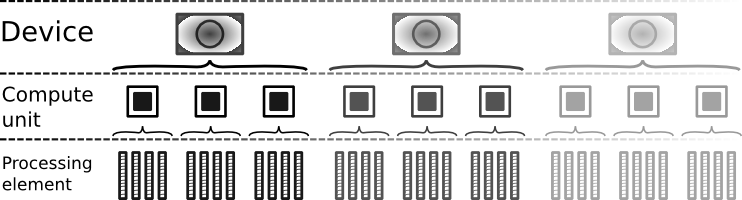
\includegraphics[scale=0.5]{../08-OpenCL/figs/platform.png}
\caption{The hierarchy defined by the OpenCL platform model.
A platform consists of multiple devices, each having multiple compute units. Whereas compute units can run independent threads, they can still contain multiple processing elements.
The memory model (\ref{sec:OpenCL:memmodel}) will also fit in this hierarchy, with (from the top) global, local and private memory residing close to corresponding layer.}
\label{fig:OpenCL:platform}
\end{center}
\end{figure}


\subsection{Execution model}
Parallel code is written in its own language `.cl', a subset of the C99 standard, where functions callable from the host are called kernels.
This code is then compiled for an already initialized device, and submitted to a command queue.
The command queue is now responsible for running this kernel once the device is ready. 
It is possible to submit multiple kernels to a queue and manage their execution via events.

\paragraph*{}
Every time a kernel is queued a virtual grid, NDRange, will be defined.
For every grid point, the kernel will be executed once.
This is how parallelism is achieved in OpenCL.
An NDRange can be one, two or three dimensional, and the size can be chosen arbitrarily up to a limit defined by the device.

The entire global grid is divided into smaller local grids called work-groups.
An illustration of a 27x27 `2DRange' composed of nine 9x9 workgroups is found in fig.~\ref{fig:OpenCL:ndrange}.
During execution each work-item will fill one processing element.
All work-items within the same work-group will run concurrently, but on the same compute unit. The other work-groups will run on other compute units within the same device.

\begin{figure}
\begin{center}
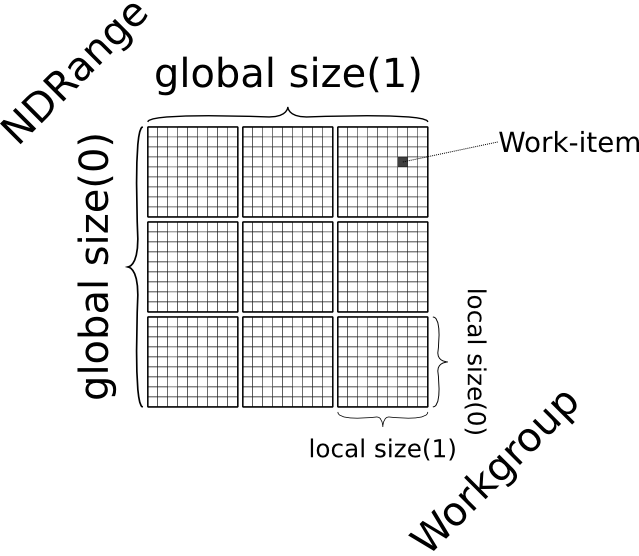
\includegraphics[scale=0.5]{../08-OpenCL/figs/NDRange.png}
\caption{A global two dimensional 27x27 NDRange. It is divided into nine work-groups, each having 9x9 work-items.}
\label{fig:OpenCL:ndrange}
\end{center}
\end{figure}



\subsection{Memory model}
\label{sec:OpenCL:memmodel}
There are four different regions for OpenCL memory:
\begin{itemize}
\item \textbf{Global} memory is allocated by the host. Both the kernel and the host have read/write access. Global memory is in general the slowest type of memory, but compensates with the largest memory size. Ideal for storing input, results or large datasets.
\item \textbf{Constant} memory is allocated by the host, with read-only access from a kernel. Often used when passing many parameters/options as one struct to the kernel.
\item \textbf{Local} memory could be allocated either dynamically by the host or statically inside a kernel. Every work group has its own independent copy of local memory, shared among the work-items inside the group. Residing close to each compute unit this memory is faster than global. 
\item \textbf{Private} memory is allocated statically by each work-item and not shared at all. Being close to the processing elements it is the fastest memory. Variables declared in kernels without specifying memory region are private by default.
\end{itemize}
A quick summary of the different memory regions can be found in table~\ref{tab:OpenCL:memory}.

\begin{table}
\begin{center}
\begin{tabular}{c|cc|cc|cc|cc}
& \multicolumn{2}{c|}{Global} & \multicolumn{2}{c|}{Constant} & \multicolumn{2}{c|}{Local} & \multicolumn{2}{c}{Private}\\
& Host & Kernel& Host & Kernel& Host & Kernel& Host & Kernel \\
\hline
Allocation & Dyn & NA & Dyn & NA & Dyn & Stat & NA & Stat\\ 
Access & R/W & R/W & R/W & R & NA & R/W & NA & R/W\\ 
\hline 
\end{tabular} 
\caption{Overview of different OpenCL memory regions. R/W: read and write. R: read only. Dyn/Stat: dynamic/static. NA: not available.}
\label{tab:OpenCL:memory}
\end{center}
\end{table}



\subsection{Programming model}
OpenCL focuses on a data parallel programming model.
Here we have multiple memory objects that can be calculated or altered by the same set of instructions. 
Instead of using loops or nested loops, our problem can be simplified by choosing appropriate global and local sizes, as we shall see for general matrix multiplication in section~\ref{sec:OpenCL:matmult}.
Task parallel programming, and hybrids between these two, are also supported. 
GPUs however favors the data parallel model, due to their SIMD architecture.

SIMD, single instruction multiple data, is a type of parallel hardware where the same instruction is performed on different sets of data at the same time.
A radeonhd 6970 consists of 64 processing elements within each compute unit, a SIMD core.
All 64 processing elements are required to do the same operations at all times, only differing by what data they are working on.
A work-group maps to one SIMD core, thus it is unfavorable to let work-items within a work-group branch by for instance an if statement.






\section{Matrix multiplication}
\label{sec:OpenCL:matmult}
The coupled-cluster code has its bottleneck in matrix-matrix multiplication.
Take for instance the second term of \eqref{eq:CC:t2eq},
\begin{equation}
t_{ij}^{ab} \leftarrow \frac{1}{2} \langle ab||de \rangle t^{de}_{ij} .
\end{equation}
Gathering indices $a,b \rightarrow \xi$, $d,e \rightarrow \xi'$ and finally $i,j \rightarrow \mu$, it can be rewritten as
\begin{equation}
t_{\xi \mu} \leftarrow \frac{1}{2} \sum_{\mu'} \langle \xi||\xi' \rangle t_{\xi' \mu} ,
\end{equation}
which is, apart from the factor $\frac{1}{2}$, identical to the mathematical definition of matrix multiplication,
\begin{equation}
\label{eq:OpenCL:matmult_def}
C_{ij} = \sum_k A_{ik} B_{kj},
\hspace{10mm}
A \in \mathbf{R}^{m\times p}, B \in \mathbf{R}^{p\times n}, C \in \mathbf{R}^{m\times n}.
\end{equation}
Element $C_{ij}$ is here the inner product of row $i$ in $A$ and column $j$ in $B$, as illustrated in fig.~\ref{fig:OpenCL:matmult}.
\begin{figure}
\begin{center}
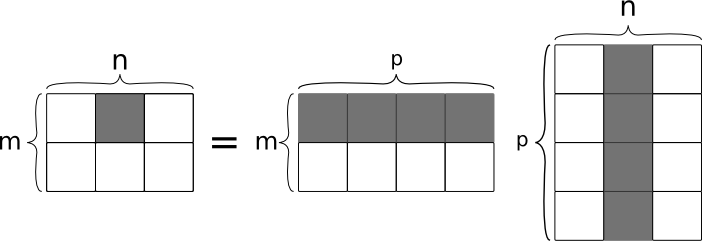
\includegraphics[scale=0.5]{../08-OpenCL/figs/matmult.png}
\caption{Outline of matrix multiplication, following its straight forward mathematical definition.}
\label{fig:OpenCL:matmult}
\end{center}
\end{figure}

\paragraph{}
To illustrate the cl language we consider a simple implementation for matrix multiplication.
In listing~\ref{lst:OpenCL:matmult_simple} we have a kernel taking three parameters, the matrices $A$, $B$ and $C$, where $A$ is already transposed.
The problem is divided into one work-item for each value of $i$ and $j$, each running the sum defined in~\eqref{eq:OpenCL:matmult_def}.
Running on a CPU this would be a good way to parallelize matrix multiplication.
The GPU, however, would be penalized by slow memory access from global memory.
\begin{lstlisting}[float,caption={Simple matrix multiplication in OpenCL. The matrices $A$, $B$ and $C$ refers to the same matrices as in eq.~\eqref{eq:OpenCL:matmult_def}. The left matrix, $A$ is already transposed, `A\_tr', to improve access pattern.},label={lst:OpenCL:matmult_simple}]
typedef double fp;

kernel void
matmult(global fp* A_tr, global fp* B, global fp* C)
{
    //WI global id (x,y)=(i,j)
    int2 gid = (int2) (get_global_id(0), get_global_id(1));

    //Calculate C_ij
    fp C_ij = 0;
    for (int k = 0; k < SIZE_P; k++)
        C_ij += A_tr[gid.x * SIZE_P + k] 
                * B[gid.y * SIZE_P + k];

    //Store into global memory again
    C[gid.x + gid.y * SIZE_M] = C_ij;
}
\end{lstlisting}


A way to improve memory access is to express the problem as multiplication of matrix-blocks. 
Figure~\ref{fig:OpenCL:matmult_loc} shows how one block in the $C$ matrix is the sum of the matrix product of blocks in $A$ and $B$. 
We set the block size to the same as the work-group size and use a 2DRange with the same dimensionality as $C$.
Each work-item is now responsible for reading one element from $A$ and one element from $B$ into the local blocks, before summing over elements in local memory.
After the sum corresponding to block multiplication is done, next block is loaded into local memory and so on.
A complete implementation is included in listing~\ref{lst:OpenCL:matmult_local}.
All work-items must complete loading from memory before any other work-item begin the summation, ensured by inserting a barrier.
We must also prevent any work-item to start loading next block until all work-items are done using the current block.
Thus we have two barriers, and one should note that barriers in OpenCL can only be applied within the same work-group.
Using local memory we have reduced the number of times matrix elements need to be transfered from global memory.
\begin{lstlisting}[float,caption={Matrix multiplication in OpenCL using local memory. The matrices $A$, $B$ and $C$ refers to the same matrices as in eq.~\eqref{eq:OpenCL:matmult_def}.},label={lst:OpenCL:matmult_local}]
typedef double fp;

kernel void
matmult(global fp* A_glb, global fp* B_glb, global fp* C_glb)
{
 //WI global id (x,y)=(i,j)
 int2 gid = (int2) (get_global_id(0), get_global_id(1));
 //Local id (x,y)
 int2 lid = (int2) (get_local_id(0), get_local_id(1));

 //Local storage for blocks.    
 local fp A[BL_SIZ][BL_SIZ];
 local fp B[BL_SIZ][BL_SIZ];
    
 //Element for this WI
 fp C_ij = 0;
  
 //Loop over blocks
 for(int k_block = 0; k_block < SIZ_P; k_block += BL_SIZ)
 {
   //Read blocks of A and B
   barrier(CLK_LOCAL_MEM_FENCE);
   A[lid.x][lid.y] = A_glb[gid.x + (k_block+lid.y) * SIZ_M];
   B[lid.x][lid.y] = B_glb[(k_block+lid.x) + gid.y * SIZ_P];
   	
   //Block multiplication
   barrier(CLK_LOCAL_MEM_FENCE);
   for(int k_loc = 0; k_loc < BL_SIZ; k_loc++)
     C_ij += A[lid.x][k_loc] * B[k_loc][lid.y];
 }

 //Store into global memory again
 C[gid.x + gid.y * SIZE_M] = C_ij;
}
\end{lstlisting}
\begin{figure}
\begin{center}
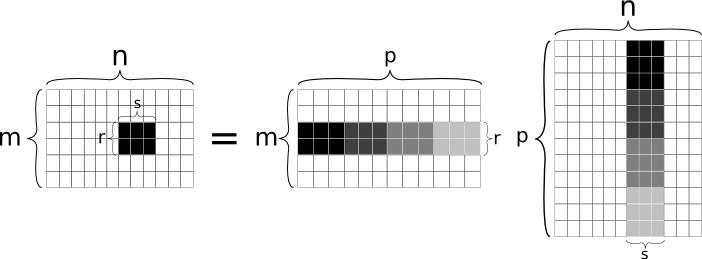
\includegraphics[scale=0.5]{../08-OpenCL/figs/matmult_loc.png}
\caption{Outline of blocked matrix multiplication.}
\label{fig:OpenCL:matmult_loc}
\end{center}
\end{figure}


The two examples of matrix multiplication shown here are not optimal solutions.
The first is quite inefficient and the second is not flexible, since the matrix sizes are limited by the block size.
AMD has developed its own BLAS library for GPUs, AMD APPML, which is both faster and more flexible.



\subsection{Strassen's algorithm}
The straightforward algorithm for matrix multiplication will require $p$ multiplications and $p-1$ additions for each of the $m\times n$ elements. The total number of floating-point operations is then $mn(2p-1) \sim \mathcal{O}(mnp)$. When the matrices $A$ and $B$ can be divided into four equally sized blocks,
\begin{equation}
\begin{bmatrix}
C_{11} & C_{12} \\
C_{21} & C_{22}
\end{bmatrix}
=
\begin{bmatrix}
A_{11} & A_{12} \\
A_{21} & A_{22} 
\end{bmatrix}
\begin{bmatrix}
B_{11} & B_{12} \\
B_{21} & B_{22}
\end{bmatrix} ,
\end{equation}
we get eight multiplications of smaller blocks,
\begin{equation}
\begin{bmatrix}
C_{11} & C_{12} \\
C_{21} & C_{22}
\end{bmatrix}
=
\begin{bmatrix}
A_{11} B_{11} + A_{12} B_{21} & A_{11} B_{12} + A_{12} B_{22} \\
A_{21} B_{11} + A_{22} B_{21} & A_{21} B_{12} + A_{22} B_{22} 
\end{bmatrix}
.
\end{equation}


Strassen discovered in 1968 how the number of multiplications could be reduced from eight to seven~\cite{springerlink:10.1007/BF02165411}.
Following Winograd's approach we define some intermediates,
\begin{equation}
\label{eq:OpenCL:Strassen_intermediates}
\begin{matrix}
S_1 = A_{21} + A_{22}, & T_1 = B_{12} - B_{11},\\
S_2 = S_1 - A_{11}, & T_2 = B_{22} - T_1,\\
S_3 = A_{11} - A_{21}, & T_3 = B_{22} - B_{12},\\
S_4 = A_{12} - S_2, & T_4 = B_{21} - T_2 ,
\end{matrix}
\end{equation}
and need seven multiplications,
\begin{equation}
\label{eq:OpenCL:Strassen_multiplications}
\begin{matrix}
P_1 &= A_{11} B_{11}, & U_1 = P_1 + P_2, \\
P_2 &= A_{12} B_{21}, & U_2 = P_1 + P_4, \\
P_3 &= S_1 T_1, & U_3 = U_2 + P_5,\\
P_4 &= S_2 T_2, & U_4 = U_3 + P_7,\\
P_5 &= S_3 T_3, & U_5 = U_3 + P_3,\\
P_6 &= S_4 B_{22}, & U_6 = U_2 + P_3,\\
P_7 &= A_{22} T_4, & U_7 = U_6 + P_6 ,
\end{matrix} 
\end{equation}
to find the resulting $C$ matrix as
\begin{equation}
\begin{bmatrix}
C_{11} & C_{12} \\
C_{21} & C_{22}
\end{bmatrix}
=
\begin{bmatrix}
U_1 & U_7 \\
U_4 & U_5 
\end{bmatrix}
.
\end{equation}
Despite the seemingly additional work, we have reduced the number of multiplications from 8 to 7. Since the multiplications are the computational bottleneck compared to addition and subtraction, the number of flops are reduced.

\paragraph{}
In the case of square $n\times n$ matrices with $n$ equal to a power of two, $n=2^m$, the divided blocks will have $\frac{n}{2} = 2^{m-1}$.
Letting $f(m)$ be the number of flops needed for the full matrix and applying Strassen recursively we find the total number of flops to be
\begin{equation}
f(m) = 7 f(m-1) = 7^2 f(m-2) = \cdots = 7^m f(0) , 
\end{equation}
where $f(0)$ is the one floating-point operation needed for multiplication of two numbers (two $2^0\times 2^0$ matrices).
For large matrices this can prove efficient, yielding a much better scaling, 
\begin{equation}
\mathcal{O}\left( 7^m \right) = 
\mathcal{O}\left( 2^{\log_2 7^m} \right) = 
\mathcal{O}\left( 2^{m \log_2 7} \right) = 
\mathcal{O}\left( n^{\log_2 7} \right) \approx
\mathcal{O}\left( n^{2.807} \right) ,
\end{equation}
effectively saving $7/8 = 12.5\%$ each time it is applied.






\section{Implementation}
Matrix multiplication has been considered an important aspect of this thesis, and all functionality has been implemented in a separate object called `GEMM' -- GEneral Matrix Multiplication.
The default implementation, demonstrated in listing~\ref{lst:OpenCL:GEMMdefault}, performs the matrix operation, 
\begin{equation}
C_{(res)} = \alpha A_{(left)} B_{(right)} + \beta C_{(res)} , 
\end{equation}
where the variable names used in the implementation are denoted in the subscript of the matrices.
When `transL' and/or `transR' is set to true $A_{(left)}$ and/or $B_{(right)}$ will be transposed before used.
Armadillo's default operations will be used in `GEMM', most likely translated into calls to some BLAS library.
Netlib~\cite{netlibblas} and GotoBLAS2~\cite{Goto:2008:HIL:1377603.1377607} are the two implementations we have tested here.
\begin{lstlisting}[float,label={lst:OpenCL:GEMMdefault},caption={GEMM default implementation.}]
virtual void dgemm(
        arma::mat &res,
        arma::mat const &left,
        arma::mat const &right,
        double alpha = 1,
        double beta = 0,
        bool transL = false,
        bool transR = false)
{
    timer.tic();
    if (transL == false && transR == false)
        res = alpha * left * right + beta * res;
    else if (transL == true && transR == false)
        res = alpha * trans(left) * right + beta * res;
    else if (transL == false && transR == true)
        res = alpha * left * trans(right) + beta * res;
    else if (transL == true && transR == true)
        res = alpha * trans(left) * trans(right) + beta * res;
    tot_time += timer.toc();

    return;
}
\end{lstlisting}

To take advantage of different implementations all C++ statements for matrix multiplication needs to be replaced with a call to a `GEMM' derived class.
As an example the second term from the coupled-cluster $\hat{T}_2$ equations, eq.~\eqref{eq:CC:t2_t2_diag}, will now be written as 
\begin{equation}
\langle \xi | t'_2 | \mu \rangle_{(\lambda)} = \alpha \sum_{\xi'} \langle \xi || \xi' \rangle_{(\lambda)} \langle \xi' |t_2| \mu \rangle_{(\lambda)} + \beta \langle \xi | t'_2 | \mu \rangle_{(\lambda)},
\end{equation}
with $\alpha = \frac{1}{2}$ and $\beta = 1$.
Implementing this listing~\ref{lst:CC:c_t2_t2} is altered slightly, as depicted in listing~\ref{lst:OpenCL:c_t2_t2}.
\begin{lstlisting}[float,label={lst:OpenCL:c_t2_t2},caption={Second term of the coupled-cluster $\hat{T}_2$ equations, now using the matrix-multiplication framework in `GEMM'.}]
for (int lmd = 0; lmd < basis->dim_lmd_2p(); lmd++)
    mult->dgemm(     //mult points to a GEMM derived object
       t2_new.at(lmd),              //Result
       sys->get_v_pppp()->at(lmd),  //Left
       t2_old.at(lmd),              //Right
       0.5, 1);                     //alpha, beta
\end{lstlisting}

Also incorporated is a system for measuring the amount of time that is used on multiplication.
A protected member, timer, of type `arma::wall\_clock', is included as well as a double, tot\_time, to record how much time is spent inside the `dgemm' method.
To get this information one simply calls `get\_tot\_time()', returning the number of seconds elapsed.


\subsection{Strassen}
`Strassen' subclasses `GEMM' and adds the method `strassenMethod' returning the matrix product of two matrices, `left' and `right', using the Strassen method.
The Strassen method is applied recursively.
An integer, `depth', is set to $0$ for the first call, and it is raised by one each time a new level of recursion is performed.
This allows us to abort recursions at a specific level, helpful when timing whether blas routines or another level of recursion is the most beneficial for a specific size of the matrices.

The `dgemm' function is overridden as in listing~\ref{lst:OpenCL:Strassen_dgemm}, essentially the same as for the default base-class implementation except now using the new \mbox{`strassenMethod'}.
\begin{lstlisting}[float,label={lst:OpenCL:Strassen_dgemm},caption={Strassen overrides the `dgemm' method.}]
timer.tic();
if (transL == false && transR == false)
  res = alpha * strassenMethod(left, right, 0) 
       + beta * res;
else if (transL == true && transR == false)
  res = alpha * strassenMethod(trans(left), right, 0) 
       + beta * res;
else if (transL == false && transR == true)
  res = alpha * strassenMethod(left, trans(right), 0) 
       + beta * res;
else if (transL == true && transR == true)
  res = alpha * strassenMethod(trans(left), trans(right), 0) 
  	   + beta * res;
tot_time += timer.toc();

return;
\end{lstlisting}
In \mbox{`strassenMethod'} the criterion for adding one level of recursion or invoking an underlying blas library is 
\begin{equation}
\label{eq:OpenCL:recursCriterion}
3 m n p < \tau \left( mn + np + pm \right),
\end{equation}
reduced to 
\begin{equation}
n < \tau
\end{equation}
in the case of equally sized square matrices, $m=n=p$.
Such a criterion was first proposed by Higham in 1990~\cite{Higham:1990:EFM:98267.98290}.
Other criteria exist but this was chosen because only one variable, $\tau$, needs to be tuned.
We estimate $\tau$ empirically by measuring the time a regular `dgemm' routine uses compared to doing one Strassen recursion for different sizes $m, n$ and $p$.


The first part of `strassenMethod', listing~\ref{lst:OpenCL:Strassen_p1}, defines some integer values needed, `m', `n' and `p' hold the size of the matrices, and `m2', `n2' and `p2' store half their size.
`dp1' is the current recursion level plus one.
If one of the dimensions is less than two it is not possible to split the matrices further, and if the recursion criterion, eq.~\eqref{eq:OpenCL:recursCriterion}, is not met it is not beneficial to split the matrices either.
These conditions are tested for, and regular multiplication through armadillo will then be used instead.
\begin{lstlisting}[float,label={lst:OpenCL:Strassen_p1},caption={Implementation of Strassen's method. Continued in listing~\ref{lst:OpenCL:Strassen_p2}.},name={strassen_complete}]
mat Strassen::strassenMethod(
	const mat& left, 
	const mat& right, 
	int depth)	 {
//Needed integer values
int m = left.n_rows;
int m2 = m / 2;
int n = right.n_cols;
int n2 = n / 2;
int p = left.n_cols;
int p2 = p / 2;
int dp1 = depth + 1;

//Criterion for further recursion. Tau is a class member (double)
if (m < 2 || n < 2 || p < 2 || (3.0 * m * n * p) / (((double) n) * p + ((double) m) * n + ((double) m) * p) < tau)
{
  return left * right;
}
\end{lstlisting}


The second part, in listing~\ref{lst:OpenCL:Strassen_p2}, deals with situations where matrices may have odd dimensions, and thus not suitable for the Strassen algorithm.
We deal with these situations using dynamic peeling.
The odd rows and columns are treated separately,
\begin{equation}
\begin{bmatrix}
C_{11}  & c_{12} \\
c_{21}  & c_{22}
\end{bmatrix}
=
\begin{bmatrix}
A_{11} & a_{12} \\
a_{21} & a_{22} 
\end{bmatrix}
\begin{bmatrix}
B_{11} & b_{12} \\
b_{21} & b_{22} 
\end{bmatrix}
= 
\begin{bmatrix}
A_{11}B_{11} + a_{12}b_{21}  & A_{11}b_{12} + a_{12}b_{22} \\
a_{21}B_{11} + a_{22}b_{21}  & a_{21}b_{12} + a_{22}b_{22} 
\end{bmatrix} , 
\end{equation}
where $A_{11}$, $B_{11}$ and $C_{11}$ now are the largest possible blocks with even dimensions.
We then have one multiplication,
\begin{equation}
C_{11} = A_{11}B_{11} , 
\end{equation}
suitable for another level of Strassen, and in the end a few fix-up steps,
\begin{equation}
\begin{split}
C_{11} =&  a_{12}b_{21}  + C_{11} \\
c_{12} =& A_{11}b_{12} + a_{12}b_{22} \\
c_{21} =& a_{21}B_{11} + a_{22}b_{21} \\
c_{22} =& a_{21}b_{12} + a_{22}b_{22} ,
\end{split}
\end{equation}
where all steps may not be needed if only some of the dimensions are odd.
\begin{lstlisting}[float,label={lst:OpenCL:Strassen_p2},caption={Implementation of Strassen's method. Continuation of listing~\ref{lst:OpenCL:Strassen_p1} and continued in listing~\ref{lst:OpenCL:Strassen_p2}.},name={strassen_complete}]
else if (m % 2 != 0 || n % 2 != 0 || p % 2 != 0) 
{
  span m2Div2(0, m2 * 2 - 1); //Spanning all elements
  span n2Div2(0, n2 * 2 - 1); //except the last, if
  span p2Div2(0, p2 * 2 - 1); //the total number is odd.
  span lastM(m - 1, m - 1); //Spanning 
  span lastN(n - 1, n - 1); //the last
  span lastP(p - 1, p - 1); //element.

  mat C(m, n);
  C(m2Div2, n2Div2) = strassenMethod(left(m2Div2, p2Div2), right(p2Div2, n2Div2), depth);

  if (p % 2 != 0) //C_11 += a_12 b_21
    C(m2Div2, n2Div2) += left(m2Div2, lastP) * right(lastP, n2Div2);

  if (n % 2 != 0)
  {	//c_12 = A_11 b_12
    C(m2Div2, lastN) = left(m2Div2, p2Div2) * right(p2Div2, lastN);

    if (p % 2 != 0)  //c_12 += a_12 b_22
      C(m2Div2, lastN) += left(m2Div2, lastP) * right(lastP, lastN);        
  }

  if (m % 2 != 0)
  {	//c_21 = a_21 B_11
    C(lastM, n2Div2) = left(lastM, p2Div2) * right(p2Div2, n2Div2);

    if (p % 2 != 0)  //c_21 += a_22 b_21
      C(lastM, n2Div2) += left(lastM, lastP) * right(lastP, n2Div2);
  }

  if (m % 2 != 0 && n % 2 != 0)
  {	//c_22 = a_21 b_12
    C(lastM, lastN) = left(lastM, p2Div2) * right(p2Div2, lastN);

    if (p % 2 != 0)  //c_22 += a_22 b_22
      C(lastM, lastN) += left(lastM, lastP) * right(lastP, lastN);
  }

  return C;
}
\end{lstlisting}






The third and last part of our Strassen implementation, listing~\ref{lst:OpenCL:Strassen_p3}, carries out the actual Strassen algorithm, implemented straight forward from the equations~\eqref{eq:OpenCL:Strassen_intermediates} and~\eqref{eq:OpenCL:Strassen_multiplications}.
\begin{lstlisting}[float,label={lst:OpenCL:Strassen_p3},caption={Implementation of Strassen's method. Continuation of listing~\ref{lst:OpenCL:Strassen_p2}.},name={strassen_complete}]
else
{
 //left matrix
 span lR1(0, m2 - 1); //First half of rows
 span lR2(m2, m - 1); //Second half of rows
 span lC1(0, p2 - 1); //First half of columns
 span lC2(p2, p - 1); //Second half of columns
 //right matrix
 span rR1(0, p2 - 1); //First half of rows
 span rR2(p2, p - 1); //Second half of rows
 span rC1(0, n2 - 1); //First half of columns
 span rC2(n2, n - 1); //Second half of columns

 //Intermediates
 mat S1 = left(lR2, lC1) + left(lR2, lC2);
 mat S2 = S1 - left(lR1, lC1);
 mat S3 = left(lR1, lC1) - left(lR2, lC1);
 mat S4 = left(lR1, lC2) - S2;
 mat T1 = right(rR1, rC2) - right(rR1, rC1);
 mat T2 = right(rR2, rC2) - T1;
 mat T3 = right(rR2, rC2) - right(rR1, rC2);
 mat T4 = right(rR2, rC1) - T2;

 //Multiplications
 mat P1 = strassenMethod(left(lR1,lC1), right(rR1,rC1), dp1);
 mat P2 = strassenMethod(left(lR1,lC2), right(rR2,rC1), dp1);
 mat P3 = strassenMethod(S1, T1, dp1);
 mat P4 = strassenMethod(S2, T2, dp1);
 mat P5 = strassenMethod(S3, T3, dp1);
 mat P6 = strassenMethod(S4, right(rR2, rC2), dp1);
 mat P7 = strassenMethod(left(lR2, lC2), T4, dp1);

 //U matrices
 mat U1 = P1 + P2;
 mat U2 = P1 + P4;
 mat U3 = U2 + P5;
 mat U4 = U3 + P7;
 mat U5 = U3 + P3;
 mat U6 = U2 + P3;
 mat U7 = U6 + P6;

 //Fill and return the result
 mat C(m, n);
 C(lR1, rC1) = U1;
 C(lR1, rC2) = U7;
 C(lR2, rC1) = U4;
 C(lR2, rC2) = U5;
 return C;
} //End of if-else
 
} //End of method
\end{lstlisting}







\subsection{CLgemm}
Matrix multiplication on GPUs through OpenCL is managed by AMD's own library, APPML (Accelerated Parallel Processing Math Libraries).
Again the `dgemm' method is altered to use a separate function for the product itself, this time implemented in `clmult'.

The overhead when using GPUs is substantial, and we need to empirically find where a CPU implementation is more efficient.
We have chosen the simplest criterion, whenever the amount of floating point operations needed is less than a threshold value armadillo's underlying functionality is used instead.
Listing~\ref{lst:OpenCL:CLgemm_p1} shows how we find the number of flops required in `clmult', and decide whether the CPU or GPU is best suited.
If there is enough work to be done data will be pushed to the graphics card followed by invoking the routine `clAmdBlasDgemm' to calculate the matrix product, as shown in listing~\ref{lst:OpenCL:CLgemm_p2}.

\begin{lstlisting}[float,label={lst:OpenCL:CLgemm_p1},caption={Implementation of matrix multiplication on a GPU. Continued in listing~\ref{lst:OpenCL:CLgemm_p2}.},name={CLgemm}]
mat CLgemm::clmult(mat const &left, mat const &right) {

int m = left.n_rows;  //Size 
int n = right.n_cols; //of input
int p = left.n_cols;  //matrices.

mat res = zeros<mat > (m, n); //Result

//Flops ~O(mnp)
double work = ((double) m) * n * p;

//Don't use GPU if few flops are required.
//This threshould value is found empirically 
//by testing where GPUs are quicker than CPUs.
if (work < 3e8)
  res = left * right;
\end{lstlisting}
\begin{lstlisting}[float,label={lst:OpenCL:CLgemm_p2},caption={Implementation of matrix multiplication on a GPU. Continuation of listing~\ref{lst:OpenCL:CLgemm_p1}},name={CLgemm}]    
else
{
  //memptr cannot be const in cl.
  cl_double *A_p = const_cast<double *> (left.memptr());
  cl_double *B_p = const_cast<double *> (right.memptr());
  cl_double *C_p = res.memptr();
  
  //Create CL buffers, copying Host memory.
  cl::Buffer A_cl(context, CL_MEM_READ_ONLY | CL_MEM_COPY_HOST_PTR, sizeof (*A_p) * left.n_elem, A_p);
  cl::Buffer B_cl(context, CL_MEM_READ_ONLY | CL_MEM_COPY_HOST_PTR, sizeof (*B_p) * right.n_elem, B_p);
  cl::Buffer C_cl(context, CL_MEM_READ_WRITE | CL_MEM_COPY_HOST_PTR, sizeof (*C_p) * res.n_elem, C_p);
 
  //Run DGEMM. armadillo uses columnmajor ordering.
  clAmdBlasDgemm( 
    clAmdBlasColumnMajor, clAmdBlasNoTrans, clAmdBlasNoTrans,
    m, n, p,      //Size of matrices.
    1.0, A_cl(), m, B_cl(), p,
    0.0, C_cl(), m,
    1, &queue(), 0, NULL, NULL);
  
  //Read results back into C
  queue.enqueueReadBuffer(C_cl, true, 0, sizeof (*C_p) * res.n_elem, C_p); 
}

return res;
}//End Method CLgemm::clmult
\end{lstlisting}








\subsection{CLstrassen}
Our `CLgemm' implementation will meet severe problems.
As the matrix size increases, the device will eventually run out of available memory. 
In order to solve this, the matrix needs to be partitioned into smaller blocks that can be processed one at a time.
For large matrices we also experience that applying Strassen's method on top of  AMD's APPML serves no purpose.
The GPU is more efficient than the overhead of blocking up the matrices.

For these reasons we have combined `Strassen' and `CLgemm', using the Strassen algorithm with a modified criterion, now only applying another level of recursion when the blocks are too big to fit on the GPU.
The new criterion is described by listing~\ref{lst:OpenCL:CLstrassen_criterion}, and the parameter `maxSizeCL' is found by querying the device, as in listing~\ref{lst:OpenCL:CLstrassen_maxSizeCL}.
\begin{lstlisting}[float,label={lst:OpenCL:CLstrassen_criterion},caption={CLstrassen's new criterion, compared to the original from listing~\ref{lst:OpenCL:Strassen_p1}. Another level of Strassen's algorithm is only applied if matrices are too big to fit on the GPU. Multiplications are then sent to `clmult' instead of armadillo's blas routines.}]
int m = left.n_rows;
int m2 = m / 2;
int n = right.n_cols;
int n2 = n / 2;
int p = left.n_cols;
int p2 = p / 2;

//Number of elements in the three matrices
size_t sizRes = m * n;
size_t sizLeft = m * p;
size_t sizRight = n * p;
size_t sizTOT = sizRes + sizRight + sizLeft;
//Number of bytes needed
sizTOT = sizeof (double) * sizTOT;

//Matrix small enough for Device?
if (sizTOT < maxSizeCL)
  return clmult.clmult(left, right); 
\end{lstlisting}
\begin{lstlisting}[float,label={lst:OpenCL:CLstrassen_maxSizeCL},caption={How to query the max number of bytes on a GPU device available for OpenCL.}]
cl_ulong maxmem_bytes = device.getInfo<CL_DEVICE_MAX_MEM_ALLOC_SIZE > ();
maxSizeCL = 0.9 * maxmem_bytes;
\end{lstlisting}














\part{Results}
\chapter{Results}
\label{Results}

In this chapter we start by testing whether the program code can
reproduce known solutions, and proceed by testing the energy
and variance optimization schemes. Then the results regarding the
atomic problem are presented and estimates of the computational time
dependency with number of particles are exemplified. The next and
final step is to suggest how to increase the efficiency of the code.

%********************* Testing the code *******************
%
%
\section{Testing the code}
\label{TestingTheCode}

Regarding the development of any numerical tool, the first concern is
to test whether the code has been correctly implemented. This
is usually done by considering special cases where the solutions are
already known. 
\newline
%
\newline
The Slater-determinant part of the code is validated by reproduction
of the HF results. This is realized by setting the Jastrow-factor
equal to unity, and using the Roothaan Hartree-Fock wave-functions
optimized by Clementi and Roetti, see ref. \cite{clementi1974}. In table
\ref{HFfNone} the results for some atoms are listed, and these
are in excellent agreement with the HF energies. This indicates that
the Slater determinant part of the code works the way it is supposed
to.
\newline

\begin{table}[hbtp]
\begin{center} {\large \bf Test of VMC Slater determinant} \\ 
$\phantom{a}$ \\
\begin{tabular}{ccccc}
\hline\\ 
$\phantom{AA}${\bf Atom}$\phantom{AA}$ & $\phantom{AA}${\bf HF}$\phantom{AA}$     & $\phantom{AA}${\bf VMC}$\phantom{AA}$    \\
He         &   -2.8617    & -2.8618(1)   \\
Li         &   -7.4327    & -7.4325(11)  \\   
B          &  -24.5290    & -24.534(12)  \\   
C          &  -37.6886    & -37.599(50)  \\   
Ne         &  -128.547    & -128.551(19) \\   
Ar         &  -526.817    & -526.84(15)  \\  [10pt]
\hline
\end{tabular} 
\end{center}
\caption{VMC results for a Roothaan Hartree-Fock wave-function Slater
  determinant, compared with the exact HF results of
  ref. \cite{clementi1974}.}
\label{HFfNone}
\end{table}

The correlation part was tested for a two-particle quantum dot. This
test was performed by a fellow student, ref. \cite{popsueva2004}, and
was in agreement with the analytical solution,
ref. \cite{dineykhan1997}.
\newline
%
\newline
Having tested the two main building blocks of our program, 
we turn our attention to the two different optimization schemes.
Both the energy and the variance optimization schemes are applied
to a few simple helium atom trial wave-functions. When introducing the
variational approach to the helium atom (in section
\ref{TheHeliumAtom}) we started out by a trial wave-function which is
a product of two hydrogen-like $1s$ orbitals, namely 

\begin{equation} 
  \psi_{\alpha} = e^{-\alpha (r_1+r_2)}.
\label{psiAlpha}
\end{equation}

Listed in table \ref{hydrHelium} are the results of the energies
optimized both through energy and variance optimization. Also listed
is the energy for $\alpha = 2$ which is in excellent agreement with
the exact result $-2.75$ (see section \ref{TheHeliumAtom}).
The energy optimization performed to obtain the
optimized result of $\psi_{\alpha}$ is given step by step in figure
\ref{parameterWalkAlpha}. This figure shows how we move from the
initial guess of $\alpha = 2$ and relax to the value $\alpha =
1.5875$. The energy estimate for $\alpha = 1.5875$ is $\langle
E_{\alpha} \rangle = -2.8365 \pm 0.0004$, which is in good, though not
excellent, agreement with the analytical energy minimum $\langle
E_{\alpha} \rangle = -2.85$ for $\alpha = 1.6875$ (see section
\ref{TheHeliumAtom}). In general, the energy optimization scheme
cannot be trusted completely. We will discuss this
shortly, but first we look at an extension to the trial
wave-function $\psi_{\alpha}$.
\newline


\begin{figure}[hbtp]
  % GNUPLOT: plain TeX with Postscript
\begingroup
  \catcode`\@=11\relax
  \def\GNUPLOTspecial{%
    \def\do##1{\catcode`##1=12\relax}\dospecials
    \catcode`\{=1\catcode`\}=2\catcode\%=14\relax\special}%
%
\expandafter\ifx\csname GNUPLOTpicture\endcsname\relax
  \csname newdimen\endcsname\GNUPLOTunit
  \gdef\GNUPLOTpicture(#1,#2){\vbox to#2\GNUPLOTunit\bgroup
    \def\put(##1,##2)##3{\unskip\raise##2\GNUPLOTunit
      \hbox to0pt{\kern##1\GNUPLOTunit ##3\hss}\ignorespaces}%
    \def\ljust##1{\vbox to0pt{\vss\hbox to0pt{##1\hss}\vss}}%
    \def\cjust##1{\vbox to0pt{\vss\hbox to0pt{\hss ##1\hss}\vss}}%
    \def\rjust##1{\vbox to0pt{\vss\hbox to0pt{\hss ##1}\vss}}%
    \def\stack##1{\let\\=\cr\tabskip=0pt\halign{\hfil ####\hfil\cr ##1\crcr}}%
    \def\lstack##1{\hbox to0pt{\vbox to0pt{\vss\stack{##1}}\hss}}%
    \def\cstack##1{\hbox to0pt{\hss\vbox to0pt{\vss\stack{##1}}\hss}}%
    \def\rstack##1{\hbox to0pt{\vbox to0pt{\stack{##1}\vss}\hss}}%
    \vss\hbox to#1\GNUPLOTunit\bgroup\ignorespaces}%
  \gdef\endGNUPLOTpicture{\hss\egroup\egroup}%
\fi
\GNUPLOTunit=0.1bp
{\GNUPLOTspecial{!
%!PS-Adobe-2.0
%%Title: Results/parameterWalkAlpha.tex
%%Creator: gnuplot 3.7 patchlevel 3
%%CreationDate: Sun Mar 21 14:11:32 2004
%%DocumentFonts: 
%%BoundingBox: 0 0 360 216
%%Orientation: Landscape
%%Pages: (atend)
%%EndComments
/gnudict 256 dict def
gnudict begin
/Color false def
/Solid false def
/gnulinewidth 5.000 def
/userlinewidth gnulinewidth def
/vshift -33 def
/dl {10 mul} def
/hpt_ 31.5 def
/vpt_ 31.5 def
/hpt hpt_ def
/vpt vpt_ def
/M {moveto} bind def
/L {lineto} bind def
/R {rmoveto} bind def
/V {rlineto} bind def
/vpt2 vpt 2 mul def
/hpt2 hpt 2 mul def
/Lshow { currentpoint stroke M
  0 vshift R show } def
/Rshow { currentpoint stroke M
  dup stringwidth pop neg vshift R show } def
/Cshow { currentpoint stroke M
  dup stringwidth pop -2 div vshift R show } def
/UP { dup vpt_ mul /vpt exch def hpt_ mul /hpt exch def
  /hpt2 hpt 2 mul def /vpt2 vpt 2 mul def } def
/DL { Color {setrgbcolor Solid {pop []} if 0 setdash }
 {pop pop pop Solid {pop []} if 0 setdash} ifelse } def
/BL { stroke userlinewidth 2 mul setlinewidth } def
/AL { stroke userlinewidth 2 div setlinewidth } def
/UL { dup gnulinewidth mul /userlinewidth exch def
      dup 1 lt {pop 1} if 10 mul /udl exch def } def
/PL { stroke userlinewidth setlinewidth } def
/LTb { BL [] 0 0 0 DL } def
/LTa { AL [1 udl mul 2 udl mul] 0 setdash 0 0 0 setrgbcolor } def
/LT0 { PL [] 1 0 0 DL } def
/LT1 { PL [4 dl 2 dl] 0 1 0 DL } def
/LT2 { PL [2 dl 3 dl] 0 0 1 DL } def
/LT3 { PL [1 dl 1.5 dl] 1 0 1 DL } def
/LT4 { PL [5 dl 2 dl 1 dl 2 dl] 0 1 1 DL } def
/LT5 { PL [4 dl 3 dl 1 dl 3 dl] 1 1 0 DL } def
/LT6 { PL [2 dl 2 dl 2 dl 4 dl] 0 0 0 DL } def
/LT7 { PL [2 dl 2 dl 2 dl 2 dl 2 dl 4 dl] 1 0.3 0 DL } def
/LT8 { PL [2 dl 2 dl 2 dl 2 dl 2 dl 2 dl 2 dl 4 dl] 0.5 0.5 0.5 DL } def
/Pnt { stroke [] 0 setdash
   gsave 1 setlinecap M 0 0 V stroke grestore } def
/Dia { stroke [] 0 setdash 2 copy vpt add M
  hpt neg vpt neg V hpt vpt neg V
  hpt vpt V hpt neg vpt V closepath stroke
  Pnt } def
/Pls { stroke [] 0 setdash vpt sub M 0 vpt2 V
  currentpoint stroke M
  hpt neg vpt neg R hpt2 0 V stroke
  } def
/Box { stroke [] 0 setdash 2 copy exch hpt sub exch vpt add M
  0 vpt2 neg V hpt2 0 V 0 vpt2 V
  hpt2 neg 0 V closepath stroke
  Pnt } def
/Crs { stroke [] 0 setdash exch hpt sub exch vpt add M
  hpt2 vpt2 neg V currentpoint stroke M
  hpt2 neg 0 R hpt2 vpt2 V stroke } def
/TriU { stroke [] 0 setdash 2 copy vpt 1.12 mul add M
  hpt neg vpt -1.62 mul V
  hpt 2 mul 0 V
  hpt neg vpt 1.62 mul V closepath stroke
  Pnt  } def
/Star { 2 copy Pls Crs } def
/BoxF { stroke [] 0 setdash exch hpt sub exch vpt add M
  0 vpt2 neg V  hpt2 0 V  0 vpt2 V
  hpt2 neg 0 V  closepath fill } def
/TriUF { stroke [] 0 setdash vpt 1.12 mul add M
  hpt neg vpt -1.62 mul V
  hpt 2 mul 0 V
  hpt neg vpt 1.62 mul V closepath fill } def
/TriD { stroke [] 0 setdash 2 copy vpt 1.12 mul sub M
  hpt neg vpt 1.62 mul V
  hpt 2 mul 0 V
  hpt neg vpt -1.62 mul V closepath stroke
  Pnt  } def
/TriDF { stroke [] 0 setdash vpt 1.12 mul sub M
  hpt neg vpt 1.62 mul V
  hpt 2 mul 0 V
  hpt neg vpt -1.62 mul V closepath fill} def
/DiaF { stroke [] 0 setdash vpt add M
  hpt neg vpt neg V hpt vpt neg V
  hpt vpt V hpt neg vpt V closepath fill } def
/Pent { stroke [] 0 setdash 2 copy gsave
  translate 0 hpt M 4 {72 rotate 0 hpt L} repeat
  closepath stroke grestore Pnt } def
/PentF { stroke [] 0 setdash gsave
  translate 0 hpt M 4 {72 rotate 0 hpt L} repeat
  closepath fill grestore } def
/Circle { stroke [] 0 setdash 2 copy
  hpt 0 360 arc stroke Pnt } def
/CircleF { stroke [] 0 setdash hpt 0 360 arc fill } def
/C0 { BL [] 0 setdash 2 copy moveto vpt 90 450  arc } bind def
/C1 { BL [] 0 setdash 2 copy        moveto
       2 copy  vpt 0 90 arc closepath fill
               vpt 0 360 arc closepath } bind def
/C2 { BL [] 0 setdash 2 copy moveto
       2 copy  vpt 90 180 arc closepath fill
               vpt 0 360 arc closepath } bind def
/C3 { BL [] 0 setdash 2 copy moveto
       2 copy  vpt 0 180 arc closepath fill
               vpt 0 360 arc closepath } bind def
/C4 { BL [] 0 setdash 2 copy moveto
       2 copy  vpt 180 270 arc closepath fill
               vpt 0 360 arc closepath } bind def
/C5 { BL [] 0 setdash 2 copy moveto
       2 copy  vpt 0 90 arc
       2 copy moveto
       2 copy  vpt 180 270 arc closepath fill
               vpt 0 360 arc } bind def
/C6 { BL [] 0 setdash 2 copy moveto
      2 copy  vpt 90 270 arc closepath fill
              vpt 0 360 arc closepath } bind def
/C7 { BL [] 0 setdash 2 copy moveto
      2 copy  vpt 0 270 arc closepath fill
              vpt 0 360 arc closepath } bind def
/C8 { BL [] 0 setdash 2 copy moveto
      2 copy vpt 270 360 arc closepath fill
              vpt 0 360 arc closepath } bind def
/C9 { BL [] 0 setdash 2 copy moveto
      2 copy  vpt 270 450 arc closepath fill
              vpt 0 360 arc closepath } bind def
/C10 { BL [] 0 setdash 2 copy 2 copy moveto vpt 270 360 arc closepath fill
       2 copy moveto
       2 copy vpt 90 180 arc closepath fill
               vpt 0 360 arc closepath } bind def
/C11 { BL [] 0 setdash 2 copy moveto
       2 copy  vpt 0 180 arc closepath fill
       2 copy moveto
       2 copy  vpt 270 360 arc closepath fill
               vpt 0 360 arc closepath } bind def
/C12 { BL [] 0 setdash 2 copy moveto
       2 copy  vpt 180 360 arc closepath fill
               vpt 0 360 arc closepath } bind def
/C13 { BL [] 0 setdash  2 copy moveto
       2 copy  vpt 0 90 arc closepath fill
       2 copy moveto
       2 copy  vpt 180 360 arc closepath fill
               vpt 0 360 arc closepath } bind def
/C14 { BL [] 0 setdash 2 copy moveto
       2 copy  vpt 90 360 arc closepath fill
               vpt 0 360 arc } bind def
/C15 { BL [] 0 setdash 2 copy vpt 0 360 arc closepath fill
               vpt 0 360 arc closepath } bind def
/Rec   { newpath 4 2 roll moveto 1 index 0 rlineto 0 exch rlineto
       neg 0 rlineto closepath } bind def
/Square { dup Rec } bind def
/Bsquare { vpt sub exch vpt sub exch vpt2 Square } bind def
/S0 { BL [] 0 setdash 2 copy moveto 0 vpt rlineto BL Bsquare } bind def
/S1 { BL [] 0 setdash 2 copy vpt Square fill Bsquare } bind def
/S2 { BL [] 0 setdash 2 copy exch vpt sub exch vpt Square fill Bsquare } bind def
/S3 { BL [] 0 setdash 2 copy exch vpt sub exch vpt2 vpt Rec fill Bsquare } bind def
/S4 { BL [] 0 setdash 2 copy exch vpt sub exch vpt sub vpt Square fill Bsquare } bind def
/S5 { BL [] 0 setdash 2 copy 2 copy vpt Square fill
       exch vpt sub exch vpt sub vpt Square fill Bsquare } bind def
/S6 { BL [] 0 setdash 2 copy exch vpt sub exch vpt sub vpt vpt2 Rec fill Bsquare } bind def
/S7 { BL [] 0 setdash 2 copy exch vpt sub exch vpt sub vpt vpt2 Rec fill
       2 copy vpt Square fill
       Bsquare } bind def
/S8 { BL [] 0 setdash 2 copy vpt sub vpt Square fill Bsquare } bind def
/S9 { BL [] 0 setdash 2 copy vpt sub vpt vpt2 Rec fill Bsquare } bind def
/S10 { BL [] 0 setdash 2 copy vpt sub vpt Square fill 2 copy exch vpt sub exch vpt Square fill
       Bsquare } bind def
/S11 { BL [] 0 setdash 2 copy vpt sub vpt Square fill 2 copy exch vpt sub exch vpt2 vpt Rec fill
       Bsquare } bind def
/S12 { BL [] 0 setdash 2 copy exch vpt sub exch vpt sub vpt2 vpt Rec fill Bsquare } bind def
/S13 { BL [] 0 setdash 2 copy exch vpt sub exch vpt sub vpt2 vpt Rec fill
       2 copy vpt Square fill Bsquare } bind def
/S14 { BL [] 0 setdash 2 copy exch vpt sub exch vpt sub vpt2 vpt Rec fill
       2 copy exch vpt sub exch vpt Square fill Bsquare } bind def
/S15 { BL [] 0 setdash 2 copy Bsquare fill Bsquare } bind def
/D0 { gsave translate 45 rotate 0 0 S0 stroke grestore } bind def
/D1 { gsave translate 45 rotate 0 0 S1 stroke grestore } bind def
/D2 { gsave translate 45 rotate 0 0 S2 stroke grestore } bind def
/D3 { gsave translate 45 rotate 0 0 S3 stroke grestore } bind def
/D4 { gsave translate 45 rotate 0 0 S4 stroke grestore } bind def
/D5 { gsave translate 45 rotate 0 0 S5 stroke grestore } bind def
/D6 { gsave translate 45 rotate 0 0 S6 stroke grestore } bind def
/D7 { gsave translate 45 rotate 0 0 S7 stroke grestore } bind def
/D8 { gsave translate 45 rotate 0 0 S8 stroke grestore } bind def
/D9 { gsave translate 45 rotate 0 0 S9 stroke grestore } bind def
/D10 { gsave translate 45 rotate 0 0 S10 stroke grestore } bind def
/D11 { gsave translate 45 rotate 0 0 S11 stroke grestore } bind def
/D12 { gsave translate 45 rotate 0 0 S12 stroke grestore } bind def
/D13 { gsave translate 45 rotate 0 0 S13 stroke grestore } bind def
/D14 { gsave translate 45 rotate 0 0 S14 stroke grestore } bind def
/D15 { gsave translate 45 rotate 0 0 S15 stroke grestore } bind def
/DiaE { stroke [] 0 setdash vpt add M
  hpt neg vpt neg V hpt vpt neg V
  hpt vpt V hpt neg vpt V closepath stroke } def
/BoxE { stroke [] 0 setdash exch hpt sub exch vpt add M
  0 vpt2 neg V hpt2 0 V 0 vpt2 V
  hpt2 neg 0 V closepath stroke } def
/TriUE { stroke [] 0 setdash vpt 1.12 mul add M
  hpt neg vpt -1.62 mul V
  hpt 2 mul 0 V
  hpt neg vpt 1.62 mul V closepath stroke } def
/TriDE { stroke [] 0 setdash vpt 1.12 mul sub M
  hpt neg vpt 1.62 mul V
  hpt 2 mul 0 V
  hpt neg vpt -1.62 mul V closepath stroke } def
/PentE { stroke [] 0 setdash gsave
  translate 0 hpt M 4 {72 rotate 0 hpt L} repeat
  closepath stroke grestore } def
/CircE { stroke [] 0 setdash 
  hpt 0 360 arc stroke } def
/Opaque { gsave closepath 1 setgray fill grestore 0 setgray closepath } def
/DiaW { stroke [] 0 setdash vpt add M
  hpt neg vpt neg V hpt vpt neg V
  hpt vpt V hpt neg vpt V Opaque stroke } def
/BoxW { stroke [] 0 setdash exch hpt sub exch vpt add M
  0 vpt2 neg V hpt2 0 V 0 vpt2 V
  hpt2 neg 0 V Opaque stroke } def
/TriUW { stroke [] 0 setdash vpt 1.12 mul add M
  hpt neg vpt -1.62 mul V
  hpt 2 mul 0 V
  hpt neg vpt 1.62 mul V Opaque stroke } def
/TriDW { stroke [] 0 setdash vpt 1.12 mul sub M
  hpt neg vpt 1.62 mul V
  hpt 2 mul 0 V
  hpt neg vpt -1.62 mul V Opaque stroke } def
/PentW { stroke [] 0 setdash gsave
  translate 0 hpt M 4 {72 rotate 0 hpt L} repeat
  Opaque stroke grestore } def
/CircW { stroke [] 0 setdash 
  hpt 0 360 arc Opaque stroke } def
/BoxFill { gsave Rec 1 setgray fill grestore } def
/Symbol-Oblique /Symbol findfont [1 0 .167 1 0 0] makefont
dup length dict begin {1 index /FID eq {pop pop} {def} ifelse} forall
currentdict end definefont pop
end
%%EndProlog
}}%
\GNUPLOTpicture(3600,2160)
{\GNUPLOTspecial{"
%%Page: 1 1
gnudict begin
gsave
0 0 translate
0.100 0.100 scale
0 setgray
newpath
1.000 UL
LTb
500 300 M
63 0 V
2887 0 R
-63 0 V
500 740 M
63 0 V
2887 0 R
-63 0 V
500 1180 M
63 0 V
2887 0 R
-63 0 V
500 1620 M
63 0 V
2887 0 R
-63 0 V
500 2060 M
63 0 V
2887 0 R
-63 0 V
500 300 M
0 63 V
0 1697 R
0 -63 V
795 300 M
0 63 V
0 1697 R
0 -63 V
1090 300 M
0 63 V
0 1697 R
0 -63 V
1385 300 M
0 63 V
0 1697 R
0 -63 V
1680 300 M
0 63 V
0 1697 R
0 -63 V
1975 300 M
0 63 V
0 1697 R
0 -63 V
2270 300 M
0 63 V
0 1697 R
0 -63 V
2565 300 M
0 63 V
0 1697 R
0 -63 V
2860 300 M
0 63 V
0 1697 R
0 -63 V
3155 300 M
0 63 V
0 1697 R
0 -63 V
3450 300 M
0 63 V
0 1697 R
0 -63 V
1.000 UL
LTb
500 300 M
2950 0 V
0 1760 V
-2950 0 V
500 300 L
1.000 UL
LT0
3087 1947 M
263 0 V
1016 1796 M
-18 88 V
18 88 V
1.000 UL
LT1
3087 1847 M
263 0 V
1090 1444 M
-37 88 V
-37 88 V
-37 88 V
37 88 V
1.000 UL
LT2
3087 1747 M
263 0 V
1090 1268 M
-74 88 V
74 88 V
1.000 UL
LT3
3087 1647 M
263 0 V
1090 1092 M
148 88 V
-148 88 V
1.000 UL
LT4
3087 1547 M
263 0 V
1090 916 M
295 88 V
-295 88 V
1.000 UL
LT5
3087 1447 M
263 0 V
3450 388 M
-590 88 V
-590 88 V
-590 88 V
-590 88 V
500 828 L
590 88 V
stroke
grestore
end
showpage
}}%
\put(3037,1447){\rjust{$100$ k}}%
\put(3037,1547){\rjust{$300$ k}}%
\put(3037,1647){\rjust{$900$ k}}%
\put(3037,1747){\rjust{$2.7$ M}}%
\put(3037,1847){\rjust{$8.1$ M}}%
\put(3037,1947){\rjust{$24.3$ M}}%
\put(1975,50){\cjust{Variational parameter $\alpha$}}%
\put(100,1180){%
\special{ps: gsave currentpoint currentpoint translate
270 rotate neg exch neg exch translate}%
\cstack{VMC run number}%
\special{ps: currentpoint grestore moveto}%
}%
\put(3450,200){\cjust{ 2}}%
\put(3155,200){\cjust{ 1.95}}%
\put(2860,200){\cjust{ 1.9}}%
\put(2565,200){\cjust{ 1.85}}%
\put(2270,200){\cjust{ 1.8}}%
\put(1975,200){\cjust{ 1.75}}%
\put(1680,200){\cjust{ 1.7}}%
\put(1385,200){\cjust{ 1.65}}%
\put(1090,200){\cjust{ 1.6}}%
\put(795,200){\cjust{ 1.55}}%
\put(500,200){\cjust{ 1.5}}%
\put(450,2060){\rjust{ 20}}%
\put(450,1620){\rjust{ 15}}%
\put(450,1180){\rjust{ 10}}%
\put(450,740){\rjust{ 5}}%
\put(450,300){\rjust{ 0}}%
\endGNUPLOTpicture
\endgroup
\endinput

  \caption{ Figure illustrating the step-by-step energy optimization
  routine. The plot was made optimizing $\psi_{\alpha}$, given by
  eq.~(\ref{psiAlpha}), with respect to energy.  We start out
  by an initial guess (VMC run number 0) for the parameter $\alpha$
  and move to the lowest energy estimate of the three points
  $\alpha-\delta\alpha, \alpha, \alpha+\delta\alpha$. Here the
  walker is generated by the central wave-function $\psi_{\alpha}$,
  and the energy estimates of the two local variation
  $\psi_{\alpha}-\delta\alpha$ and $\psi_{\alpha}+\delta\alpha$ are
  generated using correlated sampling.  We continue the process 
  until the parameter movement is no longer in the same general
  direction, and then increase the number of cycles and reduce the
  variation $\delta\alpha$ to narrow down the minimum search. This
  process is continued a total of six times; the number of MC cycles
  is increased (from 100 000 to 24 300 000) and the  parameter
  variation reduced (from 0.08 to 0.0025).
  }
  \label{parameterWalkAlpha}
\end{figure}

In Quantum Monte Carlo methods, a common extension to
wave-functions consisting of one-particle
orbitals is to include a Jastrow-factor. We select a
one-parameter Pad\'{e}-Jastrow (introduced in section
\ref{TheTrialWaveFunction}) for a first approximation, and 
now have two parameters $\alpha$ and $\beta$ to optimize,

\begin{equation} 
  \psi_{\alpha,\beta} = e^{-\alpha (r_1+r_2)} 
  exp(\frac{r_{ij}}{2(1 + \beta r_{ij})}).
\label{hydrHeliumJastrow}
\end{equation}

In table \ref{hydrHelium} the results of the two different
optimization schemes to this function are listed. Even though the
wave-function is simple, these results are quite good. By
comparison, the HF result given by ref. \cite{clementi1974}, is
$-2.8617$, and the 'exact' result as given by ref. \cite{hammond1994}
is $-2.9037$.
\newline

\begin{table}[hbtp]
\begin{center} {\large \bf Helium Hydrogenic Trial-Functions} \\ 
$\phantom{a}$ \\
\begin{tabular}{ccccc}
\hline\\ 
{\bf Wave-function} & $\phantom{AA}${\bf $\alpha$}$\phantom{AA}$& $\phantom{AA}${\bf $\beta$}$\phantom{AA}$&$\phantom{AA}${\bf VMC result}  \\
$\psi_{\alpha}$       &       2.0   &              &-2.7504(4)        \\   
$\psi_{\alpha}$       &     1.5875  &              &-2.8365(4)$^{(a)}$\\   
$\psi_{\alpha}$       &     1.9625  &              &-2.7707(4)$^{(b)}$\\   
$\psi_{\alpha,\beta}$ &     1.71    &     0.6625   &-2.8800(2)$^{(a)}$\\
$\psi_{\alpha,\beta}$ &     1.9525  &     0.39     &-2.8778(2)$^{(b)}$\\ [10pt] 
\hline
\end{tabular} 
\end{center}
\caption{VMC energies for He using different two different trial
  wave-functions $\psi_{\alpha}$ and $\psi_{\alpha,\beta} $, given by
  eqs.~(\ref{psiAlpha}) and (\ref{hydrHeliumJastrow}) respectively.
  Two different optimization schemes have been used; (a) energy
  optimization, (b) variance optimization.}
\label{hydrHelium}
\end{table}

Different results are obtained for the two individual optimization
schemes. The trial wave-functions, $\psi_{\alpha}$ and
$\psi_{\alpha,\beta}$, fail to incorporate the electron-nucleus cusp
condition for $\alpha \ne 2$. This results in an energy divergence when
one of the electron-nucleus distances approaches zero. On the other hand,
the electron-electron repulsion shields some of the nucleus
attraction. Therefore, the 'tails' of the orbitals should be
stretched, indicating a lower value of $\alpha$. Lowering $\alpha$
results in larger divergences near the nucleus, but at the same time
it gives a better representation of the wave-function at a distance
from the nucleus. The energy optimization scheme therefore results in
a lower value of $\alpha$ than the variance optimization.
This illustrates some of the differences of the two optimization 
schemes, but a more thorough investigation of the methods are
needed. Two important questions arises; will we arrive at the 
same minimum if we conducted a new search, and do we move towards the
actual minimum?
\newline
%
\newline
The answer to the first question is ambiguous, and is rather put as
a reminder that consistency-tests \emph{should} be provided before any
trust can be put into the results. The optimization routine must be
stable, which means that when applied to different starting points all
must relax to some small confined subspace of the parameter space.
A problem we often encountered was that the variation of the
parameters were small compared to the accuracy of the energy
estimates. Such an approach makes the routine relax to the wrong
parameter set. At the same time, increasing the accuracy requirement
reduces the efficiency of the optimization procedure. Therefore, some
experience is needed for selecting the number of MC cycles, choosing
the parameter step lengths etc. 
\newline
%
\newline
The second question - do we move toward the 'true' minimum - is
essential. The VMC energy optimization routine 
should, given a trial wave-function, find a set of parameters 
that are in the neighbourhood of the true energy minimum. Similarly,
the variance optimization scheme should arrive at a parameter set
near the true variance minimum. Finding a \emph{wrong} parameter set 
\emph{many} times does not make the procedure more correct. 
\newline

\begin{figure}[hbtp]
  % GNUPLOT: LaTeX picture with Postscript
\begingroup%
  \makeatletter%
  \newcommand{\GNUPLOTspecial}{%
    \@sanitize\catcode`\%=14\relax\special}%
  \setlength{\unitlength}{0.1bp}%
{\GNUPLOTspecial{!
%!PS-Adobe-2.0
%%Title: Results/parameterWalkHeHydrfBeta.alpha.tex
%%Creator: gnuplot 3.7 patchlevel 3
%%CreationDate: Tue Mar 23 12:47:10 2004
%%DocumentFonts: 
%%BoundingBox: 0 0 360 216
%%Orientation: Landscape
%%Pages: (atend)
%%EndComments
/gnudict 256 dict def
gnudict begin
/Color false def
/Solid false def
/gnulinewidth 5.000 def
/userlinewidth gnulinewidth def
/vshift -33 def
/dl {10 mul} def
/hpt_ 31.5 def
/vpt_ 31.5 def
/hpt hpt_ def
/vpt vpt_ def
/M {moveto} bind def
/L {lineto} bind def
/R {rmoveto} bind def
/V {rlineto} bind def
/vpt2 vpt 2 mul def
/hpt2 hpt 2 mul def
/Lshow { currentpoint stroke M
  0 vshift R show } def
/Rshow { currentpoint stroke M
  dup stringwidth pop neg vshift R show } def
/Cshow { currentpoint stroke M
  dup stringwidth pop -2 div vshift R show } def
/UP { dup vpt_ mul /vpt exch def hpt_ mul /hpt exch def
  /hpt2 hpt 2 mul def /vpt2 vpt 2 mul def } def
/DL { Color {setrgbcolor Solid {pop []} if 0 setdash }
 {pop pop pop Solid {pop []} if 0 setdash} ifelse } def
/BL { stroke userlinewidth 2 mul setlinewidth } def
/AL { stroke userlinewidth 2 div setlinewidth } def
/UL { dup gnulinewidth mul /userlinewidth exch def
      dup 1 lt {pop 1} if 10 mul /udl exch def } def
/PL { stroke userlinewidth setlinewidth } def
/LTb { BL [] 0 0 0 DL } def
/LTa { AL [1 udl mul 2 udl mul] 0 setdash 0 0 0 setrgbcolor } def
/LT0 { PL [] 1 0 0 DL } def
/LT1 { PL [4 dl 2 dl] 0 1 0 DL } def
/LT2 { PL [2 dl 3 dl] 0 0 1 DL } def
/LT3 { PL [1 dl 1.5 dl] 1 0 1 DL } def
/LT4 { PL [5 dl 2 dl 1 dl 2 dl] 0 1 1 DL } def
/LT5 { PL [4 dl 3 dl 1 dl 3 dl] 1 1 0 DL } def
/LT6 { PL [2 dl 2 dl 2 dl 4 dl] 0 0 0 DL } def
/LT7 { PL [2 dl 2 dl 2 dl 2 dl 2 dl 4 dl] 1 0.3 0 DL } def
/LT8 { PL [2 dl 2 dl 2 dl 2 dl 2 dl 2 dl 2 dl 4 dl] 0.5 0.5 0.5 DL } def
/Pnt { stroke [] 0 setdash
   gsave 1 setlinecap M 0 0 V stroke grestore } def
/Dia { stroke [] 0 setdash 2 copy vpt add M
  hpt neg vpt neg V hpt vpt neg V
  hpt vpt V hpt neg vpt V closepath stroke
  Pnt } def
/Pls { stroke [] 0 setdash vpt sub M 0 vpt2 V
  currentpoint stroke M
  hpt neg vpt neg R hpt2 0 V stroke
  } def
/Box { stroke [] 0 setdash 2 copy exch hpt sub exch vpt add M
  0 vpt2 neg V hpt2 0 V 0 vpt2 V
  hpt2 neg 0 V closepath stroke
  Pnt } def
/Crs { stroke [] 0 setdash exch hpt sub exch vpt add M
  hpt2 vpt2 neg V currentpoint stroke M
  hpt2 neg 0 R hpt2 vpt2 V stroke } def
/TriU { stroke [] 0 setdash 2 copy vpt 1.12 mul add M
  hpt neg vpt -1.62 mul V
  hpt 2 mul 0 V
  hpt neg vpt 1.62 mul V closepath stroke
  Pnt  } def
/Star { 2 copy Pls Crs } def
/BoxF { stroke [] 0 setdash exch hpt sub exch vpt add M
  0 vpt2 neg V  hpt2 0 V  0 vpt2 V
  hpt2 neg 0 V  closepath fill } def
/TriUF { stroke [] 0 setdash vpt 1.12 mul add M
  hpt neg vpt -1.62 mul V
  hpt 2 mul 0 V
  hpt neg vpt 1.62 mul V closepath fill } def
/TriD { stroke [] 0 setdash 2 copy vpt 1.12 mul sub M
  hpt neg vpt 1.62 mul V
  hpt 2 mul 0 V
  hpt neg vpt -1.62 mul V closepath stroke
  Pnt  } def
/TriDF { stroke [] 0 setdash vpt 1.12 mul sub M
  hpt neg vpt 1.62 mul V
  hpt 2 mul 0 V
  hpt neg vpt -1.62 mul V closepath fill} def
/DiaF { stroke [] 0 setdash vpt add M
  hpt neg vpt neg V hpt vpt neg V
  hpt vpt V hpt neg vpt V closepath fill } def
/Pent { stroke [] 0 setdash 2 copy gsave
  translate 0 hpt M 4 {72 rotate 0 hpt L} repeat
  closepath stroke grestore Pnt } def
/PentF { stroke [] 0 setdash gsave
  translate 0 hpt M 4 {72 rotate 0 hpt L} repeat
  closepath fill grestore } def
/Circle { stroke [] 0 setdash 2 copy
  hpt 0 360 arc stroke Pnt } def
/CircleF { stroke [] 0 setdash hpt 0 360 arc fill } def
/C0 { BL [] 0 setdash 2 copy moveto vpt 90 450  arc } bind def
/C1 { BL [] 0 setdash 2 copy        moveto
       2 copy  vpt 0 90 arc closepath fill
               vpt 0 360 arc closepath } bind def
/C2 { BL [] 0 setdash 2 copy moveto
       2 copy  vpt 90 180 arc closepath fill
               vpt 0 360 arc closepath } bind def
/C3 { BL [] 0 setdash 2 copy moveto
       2 copy  vpt 0 180 arc closepath fill
               vpt 0 360 arc closepath } bind def
/C4 { BL [] 0 setdash 2 copy moveto
       2 copy  vpt 180 270 arc closepath fill
               vpt 0 360 arc closepath } bind def
/C5 { BL [] 0 setdash 2 copy moveto
       2 copy  vpt 0 90 arc
       2 copy moveto
       2 copy  vpt 180 270 arc closepath fill
               vpt 0 360 arc } bind def
/C6 { BL [] 0 setdash 2 copy moveto
      2 copy  vpt 90 270 arc closepath fill
              vpt 0 360 arc closepath } bind def
/C7 { BL [] 0 setdash 2 copy moveto
      2 copy  vpt 0 270 arc closepath fill
              vpt 0 360 arc closepath } bind def
/C8 { BL [] 0 setdash 2 copy moveto
      2 copy vpt 270 360 arc closepath fill
              vpt 0 360 arc closepath } bind def
/C9 { BL [] 0 setdash 2 copy moveto
      2 copy  vpt 270 450 arc closepath fill
              vpt 0 360 arc closepath } bind def
/C10 { BL [] 0 setdash 2 copy 2 copy moveto vpt 270 360 arc closepath fill
       2 copy moveto
       2 copy vpt 90 180 arc closepath fill
               vpt 0 360 arc closepath } bind def
/C11 { BL [] 0 setdash 2 copy moveto
       2 copy  vpt 0 180 arc closepath fill
       2 copy moveto
       2 copy  vpt 270 360 arc closepath fill
               vpt 0 360 arc closepath } bind def
/C12 { BL [] 0 setdash 2 copy moveto
       2 copy  vpt 180 360 arc closepath fill
               vpt 0 360 arc closepath } bind def
/C13 { BL [] 0 setdash  2 copy moveto
       2 copy  vpt 0 90 arc closepath fill
       2 copy moveto
       2 copy  vpt 180 360 arc closepath fill
               vpt 0 360 arc closepath } bind def
/C14 { BL [] 0 setdash 2 copy moveto
       2 copy  vpt 90 360 arc closepath fill
               vpt 0 360 arc } bind def
/C15 { BL [] 0 setdash 2 copy vpt 0 360 arc closepath fill
               vpt 0 360 arc closepath } bind def
/Rec   { newpath 4 2 roll moveto 1 index 0 rlineto 0 exch rlineto
       neg 0 rlineto closepath } bind def
/Square { dup Rec } bind def
/Bsquare { vpt sub exch vpt sub exch vpt2 Square } bind def
/S0 { BL [] 0 setdash 2 copy moveto 0 vpt rlineto BL Bsquare } bind def
/S1 { BL [] 0 setdash 2 copy vpt Square fill Bsquare } bind def
/S2 { BL [] 0 setdash 2 copy exch vpt sub exch vpt Square fill Bsquare } bind def
/S3 { BL [] 0 setdash 2 copy exch vpt sub exch vpt2 vpt Rec fill Bsquare } bind def
/S4 { BL [] 0 setdash 2 copy exch vpt sub exch vpt sub vpt Square fill Bsquare } bind def
/S5 { BL [] 0 setdash 2 copy 2 copy vpt Square fill
       exch vpt sub exch vpt sub vpt Square fill Bsquare } bind def
/S6 { BL [] 0 setdash 2 copy exch vpt sub exch vpt sub vpt vpt2 Rec fill Bsquare } bind def
/S7 { BL [] 0 setdash 2 copy exch vpt sub exch vpt sub vpt vpt2 Rec fill
       2 copy vpt Square fill
       Bsquare } bind def
/S8 { BL [] 0 setdash 2 copy vpt sub vpt Square fill Bsquare } bind def
/S9 { BL [] 0 setdash 2 copy vpt sub vpt vpt2 Rec fill Bsquare } bind def
/S10 { BL [] 0 setdash 2 copy vpt sub vpt Square fill 2 copy exch vpt sub exch vpt Square fill
       Bsquare } bind def
/S11 { BL [] 0 setdash 2 copy vpt sub vpt Square fill 2 copy exch vpt sub exch vpt2 vpt Rec fill
       Bsquare } bind def
/S12 { BL [] 0 setdash 2 copy exch vpt sub exch vpt sub vpt2 vpt Rec fill Bsquare } bind def
/S13 { BL [] 0 setdash 2 copy exch vpt sub exch vpt sub vpt2 vpt Rec fill
       2 copy vpt Square fill Bsquare } bind def
/S14 { BL [] 0 setdash 2 copy exch vpt sub exch vpt sub vpt2 vpt Rec fill
       2 copy exch vpt sub exch vpt Square fill Bsquare } bind def
/S15 { BL [] 0 setdash 2 copy Bsquare fill Bsquare } bind def
/D0 { gsave translate 45 rotate 0 0 S0 stroke grestore } bind def
/D1 { gsave translate 45 rotate 0 0 S1 stroke grestore } bind def
/D2 { gsave translate 45 rotate 0 0 S2 stroke grestore } bind def
/D3 { gsave translate 45 rotate 0 0 S3 stroke grestore } bind def
/D4 { gsave translate 45 rotate 0 0 S4 stroke grestore } bind def
/D5 { gsave translate 45 rotate 0 0 S5 stroke grestore } bind def
/D6 { gsave translate 45 rotate 0 0 S6 stroke grestore } bind def
/D7 { gsave translate 45 rotate 0 0 S7 stroke grestore } bind def
/D8 { gsave translate 45 rotate 0 0 S8 stroke grestore } bind def
/D9 { gsave translate 45 rotate 0 0 S9 stroke grestore } bind def
/D10 { gsave translate 45 rotate 0 0 S10 stroke grestore } bind def
/D11 { gsave translate 45 rotate 0 0 S11 stroke grestore } bind def
/D12 { gsave translate 45 rotate 0 0 S12 stroke grestore } bind def
/D13 { gsave translate 45 rotate 0 0 S13 stroke grestore } bind def
/D14 { gsave translate 45 rotate 0 0 S14 stroke grestore } bind def
/D15 { gsave translate 45 rotate 0 0 S15 stroke grestore } bind def
/DiaE { stroke [] 0 setdash vpt add M
  hpt neg vpt neg V hpt vpt neg V
  hpt vpt V hpt neg vpt V closepath stroke } def
/BoxE { stroke [] 0 setdash exch hpt sub exch vpt add M
  0 vpt2 neg V hpt2 0 V 0 vpt2 V
  hpt2 neg 0 V closepath stroke } def
/TriUE { stroke [] 0 setdash vpt 1.12 mul add M
  hpt neg vpt -1.62 mul V
  hpt 2 mul 0 V
  hpt neg vpt 1.62 mul V closepath stroke } def
/TriDE { stroke [] 0 setdash vpt 1.12 mul sub M
  hpt neg vpt 1.62 mul V
  hpt 2 mul 0 V
  hpt neg vpt -1.62 mul V closepath stroke } def
/PentE { stroke [] 0 setdash gsave
  translate 0 hpt M 4 {72 rotate 0 hpt L} repeat
  closepath stroke grestore } def
/CircE { stroke [] 0 setdash 
  hpt 0 360 arc stroke } def
/Opaque { gsave closepath 1 setgray fill grestore 0 setgray closepath } def
/DiaW { stroke [] 0 setdash vpt add M
  hpt neg vpt neg V hpt vpt neg V
  hpt vpt V hpt neg vpt V Opaque stroke } def
/BoxW { stroke [] 0 setdash exch hpt sub exch vpt add M
  0 vpt2 neg V hpt2 0 V 0 vpt2 V
  hpt2 neg 0 V Opaque stroke } def
/TriUW { stroke [] 0 setdash vpt 1.12 mul add M
  hpt neg vpt -1.62 mul V
  hpt 2 mul 0 V
  hpt neg vpt 1.62 mul V Opaque stroke } def
/TriDW { stroke [] 0 setdash vpt 1.12 mul sub M
  hpt neg vpt 1.62 mul V
  hpt 2 mul 0 V
  hpt neg vpt -1.62 mul V Opaque stroke } def
/PentW { stroke [] 0 setdash gsave
  translate 0 hpt M 4 {72 rotate 0 hpt L} repeat
  Opaque stroke grestore } def
/CircW { stroke [] 0 setdash 
  hpt 0 360 arc Opaque stroke } def
/BoxFill { gsave Rec 1 setgray fill grestore } def
/Symbol-Oblique /Symbol findfont [1 0 .167 1 0 0] makefont
dup length dict begin {1 index /FID eq {pop pop} {def} ifelse} forall
currentdict end definefont pop
end
%%EndProlog
}}%
\begin{picture}(3600,2160)(0,0)%
{\GNUPLOTspecial{"
%%Page: 1 1
gnudict begin
gsave
0 0 translate
0.100 0.100 scale
0 setgray
newpath
1.000 UL
LTb
400 300 M
63 0 V
2987 0 R
-63 0 V
400 652 M
63 0 V
2987 0 R
-63 0 V
400 1004 M
63 0 V
2987 0 R
-63 0 V
400 1356 M
63 0 V
2987 0 R
-63 0 V
400 1708 M
63 0 V
2987 0 R
-63 0 V
400 2060 M
63 0 V
2987 0 R
-63 0 V
400 300 M
0 63 V
0 1697 R
0 -63 V
781 300 M
0 63 V
0 1697 R
0 -63 V
1163 300 M
0 63 V
0 1697 R
0 -63 V
1544 300 M
0 63 V
0 1697 R
0 -63 V
1925 300 M
0 63 V
0 1697 R
0 -63 V
2306 300 M
0 63 V
0 1697 R
0 -63 V
2688 300 M
0 63 V
0 1697 R
0 -63 V
3069 300 M
0 63 V
0 1697 R
0 -63 V
3450 300 M
0 63 V
0 1697 R
0 -63 V
1.000 UL
LTb
400 300 M
3050 0 V
0 1760 V
-3050 0 V
400 300 L
1.000 UL
LT0
3087 1947 M
263 0 V
1162 1708 M
20 70 V
19 71 V
19 70 V
19 71 V
1.000 UL
LT1
3087 1847 M
263 0 V
1162 1426 M
39 71 V
38 70 V
-38 71 V
-39 70 V
1.000 UL
LT2
3087 1747 M
263 0 V
1010 1145 M
76 70 V
76 71 V
77 70 V
-77 70 V
1.000 UL
LT3
3087 1647 M
263 0 V
1010 1004 M
152 70 V
-152 71 V
1.000 UL
LT4
3087 1547 M
263 0 V
1620 582 M
-305 70 V
-305 70 V
705 793 L
305 70 V
305 71 V
-305 70 V
1.000 UL
LT5
3087 1447 M
263 0 V
2840 300 M
-610 70 V
-610 71 V
-610 70 V
610 71 V
stroke
grestore
end
showpage
}}%
\put(3037,1447){\makebox(0,0)[r]{$100$ k}}%
\put(3037,1547){\makebox(0,0)[r]{$300$ k}}%
\put(3037,1647){\makebox(0,0)[r]{$900$ k}}%
\put(3037,1747){\makebox(0,0)[r]{$2.7$ M}}%
\put(3037,1847){\makebox(0,0)[r]{$8.1$ M}}%
\put(3037,1947){\makebox(0,0)[r]{$24.3$ M}}%
\put(1925,50){\makebox(0,0){Variational parameter $\alpha$}}%
\put(100,1180){%
\special{ps: gsave currentpoint currentpoint translate
270 rotate neg exch neg exch translate}%
\makebox(0,0)[b]{\shortstack{VMC run number}}%
\special{ps: currentpoint grestore moveto}%
}%
\put(3450,200){\makebox(0,0){ 2}}%
\put(3069,200){\makebox(0,0){ 1.95}}%
\put(2688,200){\makebox(0,0){ 1.9}}%
\put(2306,200){\makebox(0,0){ 1.85}}%
\put(1925,200){\makebox(0,0){ 1.8}}%
\put(1544,200){\makebox(0,0){ 1.75}}%
\put(1163,200){\makebox(0,0){ 1.7}}%
\put(781,200){\makebox(0,0){ 1.65}}%
\put(400,200){\makebox(0,0){ 1.6}}%
\put(350,2060){\makebox(0,0)[r]{ 25}}%
\put(350,1708){\makebox(0,0)[r]{ 20}}%
\put(350,1356){\makebox(0,0)[r]{ 15}}%
\put(350,1004){\makebox(0,0)[r]{ 10}}%
\put(350,652){\makebox(0,0)[r]{ 5}}%
\put(350,300){\makebox(0,0)[r]{ 0}}%
\end{picture}%
\endgroup
\endinput

  % GNUPLOT: plain TeX with Postscript
\begingroup
  \catcode`\@=11\relax
  \def\GNUPLOTspecial{%
    \def\do##1{\catcode`##1=12\relax}\dospecials
    \catcode`\{=1\catcode`\}=2\catcode\%=14\relax\special}%
%
\expandafter\ifx\csname GNUPLOTpicture\endcsname\relax
  \csname newdimen\endcsname\GNUPLOTunit
  \gdef\GNUPLOTpicture(#1,#2){\vbox to#2\GNUPLOTunit\bgroup
    \def\put(##1,##2)##3{\unskip\raise##2\GNUPLOTunit
      \hbox to0pt{\kern##1\GNUPLOTunit ##3\hss}\ignorespaces}%
    \def\ljust##1{\vbox to0pt{\vss\hbox to0pt{##1\hss}\vss}}%
    \def\cjust##1{\vbox to0pt{\vss\hbox to0pt{\hss ##1\hss}\vss}}%
    \def\rjust##1{\vbox to0pt{\vss\hbox to0pt{\hss ##1}\vss}}%
    \def\stack##1{\let\\=\cr\tabskip=0pt\halign{\hfil ####\hfil\cr ##1\crcr}}%
    \def\lstack##1{\hbox to0pt{\vbox to0pt{\vss\stack{##1}}\hss}}%
    \def\cstack##1{\hbox to0pt{\hss\vbox to0pt{\vss\stack{##1}}\hss}}%
    \def\rstack##1{\hbox to0pt{\vbox to0pt{\stack{##1}\vss}\hss}}%
    \vss\hbox to#1\GNUPLOTunit\bgroup\ignorespaces}%
  \gdef\endGNUPLOTpicture{\hss\egroup\egroup}%
\fi
\GNUPLOTunit=0.1bp
{\GNUPLOTspecial{!
%!PS-Adobe-2.0
%%Title: Results/parameterWalkHeHydrfBeta.beta.tex
%%Creator: gnuplot 3.7 patchlevel 3
%%CreationDate: Sun Mar 21 14:10:21 2004
%%DocumentFonts: 
%%BoundingBox: 0 0 360 216
%%Orientation: Landscape
%%Pages: (atend)
%%EndComments
/gnudict 256 dict def
gnudict begin
/Color false def
/Solid false def
/gnulinewidth 5.000 def
/userlinewidth gnulinewidth def
/vshift -33 def
/dl {10 mul} def
/hpt_ 31.5 def
/vpt_ 31.5 def
/hpt hpt_ def
/vpt vpt_ def
/M {moveto} bind def
/L {lineto} bind def
/R {rmoveto} bind def
/V {rlineto} bind def
/vpt2 vpt 2 mul def
/hpt2 hpt 2 mul def
/Lshow { currentpoint stroke M
  0 vshift R show } def
/Rshow { currentpoint stroke M
  dup stringwidth pop neg vshift R show } def
/Cshow { currentpoint stroke M
  dup stringwidth pop -2 div vshift R show } def
/UP { dup vpt_ mul /vpt exch def hpt_ mul /hpt exch def
  /hpt2 hpt 2 mul def /vpt2 vpt 2 mul def } def
/DL { Color {setrgbcolor Solid {pop []} if 0 setdash }
 {pop pop pop Solid {pop []} if 0 setdash} ifelse } def
/BL { stroke userlinewidth 2 mul setlinewidth } def
/AL { stroke userlinewidth 2 div setlinewidth } def
/UL { dup gnulinewidth mul /userlinewidth exch def
      dup 1 lt {pop 1} if 10 mul /udl exch def } def
/PL { stroke userlinewidth setlinewidth } def
/LTb { BL [] 0 0 0 DL } def
/LTa { AL [1 udl mul 2 udl mul] 0 setdash 0 0 0 setrgbcolor } def
/LT0 { PL [] 1 0 0 DL } def
/LT1 { PL [4 dl 2 dl] 0 1 0 DL } def
/LT2 { PL [2 dl 3 dl] 0 0 1 DL } def
/LT3 { PL [1 dl 1.5 dl] 1 0 1 DL } def
/LT4 { PL [5 dl 2 dl 1 dl 2 dl] 0 1 1 DL } def
/LT5 { PL [4 dl 3 dl 1 dl 3 dl] 1 1 0 DL } def
/LT6 { PL [2 dl 2 dl 2 dl 4 dl] 0 0 0 DL } def
/LT7 { PL [2 dl 2 dl 2 dl 2 dl 2 dl 4 dl] 1 0.3 0 DL } def
/LT8 { PL [2 dl 2 dl 2 dl 2 dl 2 dl 2 dl 2 dl 4 dl] 0.5 0.5 0.5 DL } def
/Pnt { stroke [] 0 setdash
   gsave 1 setlinecap M 0 0 V stroke grestore } def
/Dia { stroke [] 0 setdash 2 copy vpt add M
  hpt neg vpt neg V hpt vpt neg V
  hpt vpt V hpt neg vpt V closepath stroke
  Pnt } def
/Pls { stroke [] 0 setdash vpt sub M 0 vpt2 V
  currentpoint stroke M
  hpt neg vpt neg R hpt2 0 V stroke
  } def
/Box { stroke [] 0 setdash 2 copy exch hpt sub exch vpt add M
  0 vpt2 neg V hpt2 0 V 0 vpt2 V
  hpt2 neg 0 V closepath stroke
  Pnt } def
/Crs { stroke [] 0 setdash exch hpt sub exch vpt add M
  hpt2 vpt2 neg V currentpoint stroke M
  hpt2 neg 0 R hpt2 vpt2 V stroke } def
/TriU { stroke [] 0 setdash 2 copy vpt 1.12 mul add M
  hpt neg vpt -1.62 mul V
  hpt 2 mul 0 V
  hpt neg vpt 1.62 mul V closepath stroke
  Pnt  } def
/Star { 2 copy Pls Crs } def
/BoxF { stroke [] 0 setdash exch hpt sub exch vpt add M
  0 vpt2 neg V  hpt2 0 V  0 vpt2 V
  hpt2 neg 0 V  closepath fill } def
/TriUF { stroke [] 0 setdash vpt 1.12 mul add M
  hpt neg vpt -1.62 mul V
  hpt 2 mul 0 V
  hpt neg vpt 1.62 mul V closepath fill } def
/TriD { stroke [] 0 setdash 2 copy vpt 1.12 mul sub M
  hpt neg vpt 1.62 mul V
  hpt 2 mul 0 V
  hpt neg vpt -1.62 mul V closepath stroke
  Pnt  } def
/TriDF { stroke [] 0 setdash vpt 1.12 mul sub M
  hpt neg vpt 1.62 mul V
  hpt 2 mul 0 V
  hpt neg vpt -1.62 mul V closepath fill} def
/DiaF { stroke [] 0 setdash vpt add M
  hpt neg vpt neg V hpt vpt neg V
  hpt vpt V hpt neg vpt V closepath fill } def
/Pent { stroke [] 0 setdash 2 copy gsave
  translate 0 hpt M 4 {72 rotate 0 hpt L} repeat
  closepath stroke grestore Pnt } def
/PentF { stroke [] 0 setdash gsave
  translate 0 hpt M 4 {72 rotate 0 hpt L} repeat
  closepath fill grestore } def
/Circle { stroke [] 0 setdash 2 copy
  hpt 0 360 arc stroke Pnt } def
/CircleF { stroke [] 0 setdash hpt 0 360 arc fill } def
/C0 { BL [] 0 setdash 2 copy moveto vpt 90 450  arc } bind def
/C1 { BL [] 0 setdash 2 copy        moveto
       2 copy  vpt 0 90 arc closepath fill
               vpt 0 360 arc closepath } bind def
/C2 { BL [] 0 setdash 2 copy moveto
       2 copy  vpt 90 180 arc closepath fill
               vpt 0 360 arc closepath } bind def
/C3 { BL [] 0 setdash 2 copy moveto
       2 copy  vpt 0 180 arc closepath fill
               vpt 0 360 arc closepath } bind def
/C4 { BL [] 0 setdash 2 copy moveto
       2 copy  vpt 180 270 arc closepath fill
               vpt 0 360 arc closepath } bind def
/C5 { BL [] 0 setdash 2 copy moveto
       2 copy  vpt 0 90 arc
       2 copy moveto
       2 copy  vpt 180 270 arc closepath fill
               vpt 0 360 arc } bind def
/C6 { BL [] 0 setdash 2 copy moveto
      2 copy  vpt 90 270 arc closepath fill
              vpt 0 360 arc closepath } bind def
/C7 { BL [] 0 setdash 2 copy moveto
      2 copy  vpt 0 270 arc closepath fill
              vpt 0 360 arc closepath } bind def
/C8 { BL [] 0 setdash 2 copy moveto
      2 copy vpt 270 360 arc closepath fill
              vpt 0 360 arc closepath } bind def
/C9 { BL [] 0 setdash 2 copy moveto
      2 copy  vpt 270 450 arc closepath fill
              vpt 0 360 arc closepath } bind def
/C10 { BL [] 0 setdash 2 copy 2 copy moveto vpt 270 360 arc closepath fill
       2 copy moveto
       2 copy vpt 90 180 arc closepath fill
               vpt 0 360 arc closepath } bind def
/C11 { BL [] 0 setdash 2 copy moveto
       2 copy  vpt 0 180 arc closepath fill
       2 copy moveto
       2 copy  vpt 270 360 arc closepath fill
               vpt 0 360 arc closepath } bind def
/C12 { BL [] 0 setdash 2 copy moveto
       2 copy  vpt 180 360 arc closepath fill
               vpt 0 360 arc closepath } bind def
/C13 { BL [] 0 setdash  2 copy moveto
       2 copy  vpt 0 90 arc closepath fill
       2 copy moveto
       2 copy  vpt 180 360 arc closepath fill
               vpt 0 360 arc closepath } bind def
/C14 { BL [] 0 setdash 2 copy moveto
       2 copy  vpt 90 360 arc closepath fill
               vpt 0 360 arc } bind def
/C15 { BL [] 0 setdash 2 copy vpt 0 360 arc closepath fill
               vpt 0 360 arc closepath } bind def
/Rec   { newpath 4 2 roll moveto 1 index 0 rlineto 0 exch rlineto
       neg 0 rlineto closepath } bind def
/Square { dup Rec } bind def
/Bsquare { vpt sub exch vpt sub exch vpt2 Square } bind def
/S0 { BL [] 0 setdash 2 copy moveto 0 vpt rlineto BL Bsquare } bind def
/S1 { BL [] 0 setdash 2 copy vpt Square fill Bsquare } bind def
/S2 { BL [] 0 setdash 2 copy exch vpt sub exch vpt Square fill Bsquare } bind def
/S3 { BL [] 0 setdash 2 copy exch vpt sub exch vpt2 vpt Rec fill Bsquare } bind def
/S4 { BL [] 0 setdash 2 copy exch vpt sub exch vpt sub vpt Square fill Bsquare } bind def
/S5 { BL [] 0 setdash 2 copy 2 copy vpt Square fill
       exch vpt sub exch vpt sub vpt Square fill Bsquare } bind def
/S6 { BL [] 0 setdash 2 copy exch vpt sub exch vpt sub vpt vpt2 Rec fill Bsquare } bind def
/S7 { BL [] 0 setdash 2 copy exch vpt sub exch vpt sub vpt vpt2 Rec fill
       2 copy vpt Square fill
       Bsquare } bind def
/S8 { BL [] 0 setdash 2 copy vpt sub vpt Square fill Bsquare } bind def
/S9 { BL [] 0 setdash 2 copy vpt sub vpt vpt2 Rec fill Bsquare } bind def
/S10 { BL [] 0 setdash 2 copy vpt sub vpt Square fill 2 copy exch vpt sub exch vpt Square fill
       Bsquare } bind def
/S11 { BL [] 0 setdash 2 copy vpt sub vpt Square fill 2 copy exch vpt sub exch vpt2 vpt Rec fill
       Bsquare } bind def
/S12 { BL [] 0 setdash 2 copy exch vpt sub exch vpt sub vpt2 vpt Rec fill Bsquare } bind def
/S13 { BL [] 0 setdash 2 copy exch vpt sub exch vpt sub vpt2 vpt Rec fill
       2 copy vpt Square fill Bsquare } bind def
/S14 { BL [] 0 setdash 2 copy exch vpt sub exch vpt sub vpt2 vpt Rec fill
       2 copy exch vpt sub exch vpt Square fill Bsquare } bind def
/S15 { BL [] 0 setdash 2 copy Bsquare fill Bsquare } bind def
/D0 { gsave translate 45 rotate 0 0 S0 stroke grestore } bind def
/D1 { gsave translate 45 rotate 0 0 S1 stroke grestore } bind def
/D2 { gsave translate 45 rotate 0 0 S2 stroke grestore } bind def
/D3 { gsave translate 45 rotate 0 0 S3 stroke grestore } bind def
/D4 { gsave translate 45 rotate 0 0 S4 stroke grestore } bind def
/D5 { gsave translate 45 rotate 0 0 S5 stroke grestore } bind def
/D6 { gsave translate 45 rotate 0 0 S6 stroke grestore } bind def
/D7 { gsave translate 45 rotate 0 0 S7 stroke grestore } bind def
/D8 { gsave translate 45 rotate 0 0 S8 stroke grestore } bind def
/D9 { gsave translate 45 rotate 0 0 S9 stroke grestore } bind def
/D10 { gsave translate 45 rotate 0 0 S10 stroke grestore } bind def
/D11 { gsave translate 45 rotate 0 0 S11 stroke grestore } bind def
/D12 { gsave translate 45 rotate 0 0 S12 stroke grestore } bind def
/D13 { gsave translate 45 rotate 0 0 S13 stroke grestore } bind def
/D14 { gsave translate 45 rotate 0 0 S14 stroke grestore } bind def
/D15 { gsave translate 45 rotate 0 0 S15 stroke grestore } bind def
/DiaE { stroke [] 0 setdash vpt add M
  hpt neg vpt neg V hpt vpt neg V
  hpt vpt V hpt neg vpt V closepath stroke } def
/BoxE { stroke [] 0 setdash exch hpt sub exch vpt add M
  0 vpt2 neg V hpt2 0 V 0 vpt2 V
  hpt2 neg 0 V closepath stroke } def
/TriUE { stroke [] 0 setdash vpt 1.12 mul add M
  hpt neg vpt -1.62 mul V
  hpt 2 mul 0 V
  hpt neg vpt 1.62 mul V closepath stroke } def
/TriDE { stroke [] 0 setdash vpt 1.12 mul sub M
  hpt neg vpt 1.62 mul V
  hpt 2 mul 0 V
  hpt neg vpt -1.62 mul V closepath stroke } def
/PentE { stroke [] 0 setdash gsave
  translate 0 hpt M 4 {72 rotate 0 hpt L} repeat
  closepath stroke grestore } def
/CircE { stroke [] 0 setdash 
  hpt 0 360 arc stroke } def
/Opaque { gsave closepath 1 setgray fill grestore 0 setgray closepath } def
/DiaW { stroke [] 0 setdash vpt add M
  hpt neg vpt neg V hpt vpt neg V
  hpt vpt V hpt neg vpt V Opaque stroke } def
/BoxW { stroke [] 0 setdash exch hpt sub exch vpt add M
  0 vpt2 neg V hpt2 0 V 0 vpt2 V
  hpt2 neg 0 V Opaque stroke } def
/TriUW { stroke [] 0 setdash vpt 1.12 mul add M
  hpt neg vpt -1.62 mul V
  hpt 2 mul 0 V
  hpt neg vpt 1.62 mul V Opaque stroke } def
/TriDW { stroke [] 0 setdash vpt 1.12 mul sub M
  hpt neg vpt 1.62 mul V
  hpt 2 mul 0 V
  hpt neg vpt -1.62 mul V Opaque stroke } def
/PentW { stroke [] 0 setdash gsave
  translate 0 hpt M 4 {72 rotate 0 hpt L} repeat
  Opaque stroke grestore } def
/CircW { stroke [] 0 setdash 
  hpt 0 360 arc Opaque stroke } def
/BoxFill { gsave Rec 1 setgray fill grestore } def
/Symbol-Oblique /Symbol findfont [1 0 .167 1 0 0] makefont
dup length dict begin {1 index /FID eq {pop pop} {def} ifelse} forall
currentdict end definefont pop
end
%%EndProlog
}}%
\GNUPLOTpicture(3600,2160)
{\GNUPLOTspecial{"
%%Page: 1 1
gnudict begin
gsave
0 0 translate
0.100 0.100 scale
0 setgray
newpath
1.000 UL
LTb
500 300 M
63 0 V
2887 0 R
-63 0 V
500 652 M
63 0 V
2887 0 R
-63 0 V
500 1004 M
63 0 V
2887 0 R
-63 0 V
500 1356 M
63 0 V
2887 0 R
-63 0 V
500 1708 M
63 0 V
2887 0 R
-63 0 V
500 2060 M
63 0 V
2887 0 R
-63 0 V
500 300 M
0 63 V
0 1697 R
0 -63 V
795 300 M
0 63 V
0 1697 R
0 -63 V
1090 300 M
0 63 V
0 1697 R
0 -63 V
1385 300 M
0 63 V
0 1697 R
0 -63 V
1680 300 M
0 63 V
0 1697 R
0 -63 V
1975 300 M
0 63 V
0 1697 R
0 -63 V
2270 300 M
0 63 V
0 1697 R
0 -63 V
2565 300 M
0 63 V
0 1697 R
0 -63 V
2860 300 M
0 63 V
0 1697 R
0 -63 V
3155 300 M
0 63 V
0 1697 R
0 -63 V
3450 300 M
0 63 V
0 1697 R
0 -63 V
1.000 UL
LTb
500 300 M
2950 0 V
0 1760 V
-2950 0 V
500 300 L
1.000 UL
LT0
3087 1947 M
263 0 V
2683 1708 M
0 70 V
-15 71 V
-15 70 V
-14 71 V
1.000 UL
LT1
3087 1847 M
263 0 V
2742 1426 M
-30 71 V
-29 70 V
-30 71 V
30 70 V
1.000 UL
LT2
3087 1747 M
263 0 V
2860 1145 M
59 70 V
-59 71 V
-59 70 V
-59 70 V
1.000 UL
LT3
3087 1647 M
263 0 V
2860 1004 M
118 70 V
-118 71 V
1.000 UL
LT4
3087 1547 M
263 0 V
1680 582 M
236 70 V
236 70 V
236 71 V
236 70 V
236 71 V
0 70 V
1.000 UL
LT5
3087 1447 M
263 0 V
1208 300 M
736 370 L
0 71 V
472 70 V
472 71 V
stroke
grestore
end
showpage
}}%
\put(3037,1447){\rjust{$100$ k}}%
\put(3037,1547){\rjust{$300$ k}}%
\put(3037,1647){\rjust{$900$ k}}%
\put(3037,1747){\rjust{$2.7$ M}}%
\put(3037,1847){\rjust{$8.1$ M}}%
\put(3037,1947){\rjust{$24.3$ M}}%
\put(1975,50){\cjust{Variational parameter $\beta$}}%
\put(100,1180){%
\special{ps: gsave currentpoint currentpoint translate
270 rotate neg exch neg exch translate}%
\cstack{VMC run number}%
\special{ps: currentpoint grestore moveto}%
}%
\put(3450,200){\cjust{ 0.8}}%
\put(3155,200){\cjust{ 0.75}}%
\put(2860,200){\cjust{ 0.7}}%
\put(2565,200){\cjust{ 0.65}}%
\put(2270,200){\cjust{ 0.6}}%
\put(1975,200){\cjust{ 0.55}}%
\put(1680,200){\cjust{ 0.5}}%
\put(1385,200){\cjust{ 0.45}}%
\put(1090,200){\cjust{ 0.4}}%
\put(795,200){\cjust{ 0.35}}%
\put(500,200){\cjust{ 0.3}}%
\put(450,2060){\rjust{ 25}}%
\put(450,1708){\rjust{ 20}}%
\put(450,1356){\rjust{ 15}}%
\put(450,1004){\rjust{ 10}}%
\put(450,652){\rjust{ 5}}%
\put(450,300){\rjust{ 0}}%
\endGNUPLOTpicture
\endgroup
\endinput

  %% GNUPLOT: plain TeX with Postscript
\begingroup
  \catcode`\@=11\relax
  \def\GNUPLOTspecial{%
    \def\do##1{\catcode`##1=12\relax}\dospecials
    \catcode`\{=1\catcode`\}=2\catcode\%=14\relax\special}%
%
\expandafter\ifx\csname GNUPLOTpicture\endcsname\relax
  \csname newdimen\endcsname\GNUPLOTunit
  \gdef\GNUPLOTpicture(#1,#2){\vbox to#2\GNUPLOTunit\bgroup
    \def\put(##1,##2)##3{\unskip\raise##2\GNUPLOTunit
      \hbox to0pt{\kern##1\GNUPLOTunit ##3\hss}\ignorespaces}%
    \def\ljust##1{\vbox to0pt{\vss\hbox to0pt{##1\hss}\vss}}%
    \def\cjust##1{\vbox to0pt{\vss\hbox to0pt{\hss ##1\hss}\vss}}%
    \def\rjust##1{\vbox to0pt{\vss\hbox to0pt{\hss ##1}\vss}}%
    \def\stack##1{\let\\=\cr\tabskip=0pt\halign{\hfil ####\hfil\cr ##1\crcr}}%
    \def\lstack##1{\hbox to0pt{\vbox to0pt{\vss\stack{##1}}\hss}}%
    \def\cstack##1{\hbox to0pt{\hss\vbox to0pt{\vss\stack{##1}}\hss}}%
    \def\rstack##1{\hbox to0pt{\vbox to0pt{\stack{##1}\vss}\hss}}%
    \vss\hbox to#1\GNUPLOTunit\bgroup\ignorespaces}%
  \gdef\endGNUPLOTpicture{\hss\egroup\egroup}%
\fi
\GNUPLOTunit=0.1bp
{\GNUPLOTspecial{!
%!PS-Adobe-2.0
%%Title: Results/parameterWalkHeHydrfBeta.energy.tex
%%Creator: gnuplot 3.7 patchlevel 3
%%CreationDate: Sun Mar 21 14:09:52 2004
%%DocumentFonts: 
%%BoundingBox: 0 0 360 216
%%Orientation: Landscape
%%Pages: (atend)
%%EndComments
/gnudict 256 dict def
gnudict begin
/Color false def
/Solid false def
/gnulinewidth 5.000 def
/userlinewidth gnulinewidth def
/vshift -33 def
/dl {10 mul} def
/hpt_ 31.5 def
/vpt_ 31.5 def
/hpt hpt_ def
/vpt vpt_ def
/M {moveto} bind def
/L {lineto} bind def
/R {rmoveto} bind def
/V {rlineto} bind def
/vpt2 vpt 2 mul def
/hpt2 hpt 2 mul def
/Lshow { currentpoint stroke M
  0 vshift R show } def
/Rshow { currentpoint stroke M
  dup stringwidth pop neg vshift R show } def
/Cshow { currentpoint stroke M
  dup stringwidth pop -2 div vshift R show } def
/UP { dup vpt_ mul /vpt exch def hpt_ mul /hpt exch def
  /hpt2 hpt 2 mul def /vpt2 vpt 2 mul def } def
/DL { Color {setrgbcolor Solid {pop []} if 0 setdash }
 {pop pop pop Solid {pop []} if 0 setdash} ifelse } def
/BL { stroke userlinewidth 2 mul setlinewidth } def
/AL { stroke userlinewidth 2 div setlinewidth } def
/UL { dup gnulinewidth mul /userlinewidth exch def
      dup 1 lt {pop 1} if 10 mul /udl exch def } def
/PL { stroke userlinewidth setlinewidth } def
/LTb { BL [] 0 0 0 DL } def
/LTa { AL [1 udl mul 2 udl mul] 0 setdash 0 0 0 setrgbcolor } def
/LT0 { PL [] 1 0 0 DL } def
/LT1 { PL [4 dl 2 dl] 0 1 0 DL } def
/LT2 { PL [2 dl 3 dl] 0 0 1 DL } def
/LT3 { PL [1 dl 1.5 dl] 1 0 1 DL } def
/LT4 { PL [5 dl 2 dl 1 dl 2 dl] 0 1 1 DL } def
/LT5 { PL [4 dl 3 dl 1 dl 3 dl] 1 1 0 DL } def
/LT6 { PL [2 dl 2 dl 2 dl 4 dl] 0 0 0 DL } def
/LT7 { PL [2 dl 2 dl 2 dl 2 dl 2 dl 4 dl] 1 0.3 0 DL } def
/LT8 { PL [2 dl 2 dl 2 dl 2 dl 2 dl 2 dl 2 dl 4 dl] 0.5 0.5 0.5 DL } def
/Pnt { stroke [] 0 setdash
   gsave 1 setlinecap M 0 0 V stroke grestore } def
/Dia { stroke [] 0 setdash 2 copy vpt add M
  hpt neg vpt neg V hpt vpt neg V
  hpt vpt V hpt neg vpt V closepath stroke
  Pnt } def
/Pls { stroke [] 0 setdash vpt sub M 0 vpt2 V
  currentpoint stroke M
  hpt neg vpt neg R hpt2 0 V stroke
  } def
/Box { stroke [] 0 setdash 2 copy exch hpt sub exch vpt add M
  0 vpt2 neg V hpt2 0 V 0 vpt2 V
  hpt2 neg 0 V closepath stroke
  Pnt } def
/Crs { stroke [] 0 setdash exch hpt sub exch vpt add M
  hpt2 vpt2 neg V currentpoint stroke M
  hpt2 neg 0 R hpt2 vpt2 V stroke } def
/TriU { stroke [] 0 setdash 2 copy vpt 1.12 mul add M
  hpt neg vpt -1.62 mul V
  hpt 2 mul 0 V
  hpt neg vpt 1.62 mul V closepath stroke
  Pnt  } def
/Star { 2 copy Pls Crs } def
/BoxF { stroke [] 0 setdash exch hpt sub exch vpt add M
  0 vpt2 neg V  hpt2 0 V  0 vpt2 V
  hpt2 neg 0 V  closepath fill } def
/TriUF { stroke [] 0 setdash vpt 1.12 mul add M
  hpt neg vpt -1.62 mul V
  hpt 2 mul 0 V
  hpt neg vpt 1.62 mul V closepath fill } def
/TriD { stroke [] 0 setdash 2 copy vpt 1.12 mul sub M
  hpt neg vpt 1.62 mul V
  hpt 2 mul 0 V
  hpt neg vpt -1.62 mul V closepath stroke
  Pnt  } def
/TriDF { stroke [] 0 setdash vpt 1.12 mul sub M
  hpt neg vpt 1.62 mul V
  hpt 2 mul 0 V
  hpt neg vpt -1.62 mul V closepath fill} def
/DiaF { stroke [] 0 setdash vpt add M
  hpt neg vpt neg V hpt vpt neg V
  hpt vpt V hpt neg vpt V closepath fill } def
/Pent { stroke [] 0 setdash 2 copy gsave
  translate 0 hpt M 4 {72 rotate 0 hpt L} repeat
  closepath stroke grestore Pnt } def
/PentF { stroke [] 0 setdash gsave
  translate 0 hpt M 4 {72 rotate 0 hpt L} repeat
  closepath fill grestore } def
/Circle { stroke [] 0 setdash 2 copy
  hpt 0 360 arc stroke Pnt } def
/CircleF { stroke [] 0 setdash hpt 0 360 arc fill } def
/C0 { BL [] 0 setdash 2 copy moveto vpt 90 450  arc } bind def
/C1 { BL [] 0 setdash 2 copy        moveto
       2 copy  vpt 0 90 arc closepath fill
               vpt 0 360 arc closepath } bind def
/C2 { BL [] 0 setdash 2 copy moveto
       2 copy  vpt 90 180 arc closepath fill
               vpt 0 360 arc closepath } bind def
/C3 { BL [] 0 setdash 2 copy moveto
       2 copy  vpt 0 180 arc closepath fill
               vpt 0 360 arc closepath } bind def
/C4 { BL [] 0 setdash 2 copy moveto
       2 copy  vpt 180 270 arc closepath fill
               vpt 0 360 arc closepath } bind def
/C5 { BL [] 0 setdash 2 copy moveto
       2 copy  vpt 0 90 arc
       2 copy moveto
       2 copy  vpt 180 270 arc closepath fill
               vpt 0 360 arc } bind def
/C6 { BL [] 0 setdash 2 copy moveto
      2 copy  vpt 90 270 arc closepath fill
              vpt 0 360 arc closepath } bind def
/C7 { BL [] 0 setdash 2 copy moveto
      2 copy  vpt 0 270 arc closepath fill
              vpt 0 360 arc closepath } bind def
/C8 { BL [] 0 setdash 2 copy moveto
      2 copy vpt 270 360 arc closepath fill
              vpt 0 360 arc closepath } bind def
/C9 { BL [] 0 setdash 2 copy moveto
      2 copy  vpt 270 450 arc closepath fill
              vpt 0 360 arc closepath } bind def
/C10 { BL [] 0 setdash 2 copy 2 copy moveto vpt 270 360 arc closepath fill
       2 copy moveto
       2 copy vpt 90 180 arc closepath fill
               vpt 0 360 arc closepath } bind def
/C11 { BL [] 0 setdash 2 copy moveto
       2 copy  vpt 0 180 arc closepath fill
       2 copy moveto
       2 copy  vpt 270 360 arc closepath fill
               vpt 0 360 arc closepath } bind def
/C12 { BL [] 0 setdash 2 copy moveto
       2 copy  vpt 180 360 arc closepath fill
               vpt 0 360 arc closepath } bind def
/C13 { BL [] 0 setdash  2 copy moveto
       2 copy  vpt 0 90 arc closepath fill
       2 copy moveto
       2 copy  vpt 180 360 arc closepath fill
               vpt 0 360 arc closepath } bind def
/C14 { BL [] 0 setdash 2 copy moveto
       2 copy  vpt 90 360 arc closepath fill
               vpt 0 360 arc } bind def
/C15 { BL [] 0 setdash 2 copy vpt 0 360 arc closepath fill
               vpt 0 360 arc closepath } bind def
/Rec   { newpath 4 2 roll moveto 1 index 0 rlineto 0 exch rlineto
       neg 0 rlineto closepath } bind def
/Square { dup Rec } bind def
/Bsquare { vpt sub exch vpt sub exch vpt2 Square } bind def
/S0 { BL [] 0 setdash 2 copy moveto 0 vpt rlineto BL Bsquare } bind def
/S1 { BL [] 0 setdash 2 copy vpt Square fill Bsquare } bind def
/S2 { BL [] 0 setdash 2 copy exch vpt sub exch vpt Square fill Bsquare } bind def
/S3 { BL [] 0 setdash 2 copy exch vpt sub exch vpt2 vpt Rec fill Bsquare } bind def
/S4 { BL [] 0 setdash 2 copy exch vpt sub exch vpt sub vpt Square fill Bsquare } bind def
/S5 { BL [] 0 setdash 2 copy 2 copy vpt Square fill
       exch vpt sub exch vpt sub vpt Square fill Bsquare } bind def
/S6 { BL [] 0 setdash 2 copy exch vpt sub exch vpt sub vpt vpt2 Rec fill Bsquare } bind def
/S7 { BL [] 0 setdash 2 copy exch vpt sub exch vpt sub vpt vpt2 Rec fill
       2 copy vpt Square fill
       Bsquare } bind def
/S8 { BL [] 0 setdash 2 copy vpt sub vpt Square fill Bsquare } bind def
/S9 { BL [] 0 setdash 2 copy vpt sub vpt vpt2 Rec fill Bsquare } bind def
/S10 { BL [] 0 setdash 2 copy vpt sub vpt Square fill 2 copy exch vpt sub exch vpt Square fill
       Bsquare } bind def
/S11 { BL [] 0 setdash 2 copy vpt sub vpt Square fill 2 copy exch vpt sub exch vpt2 vpt Rec fill
       Bsquare } bind def
/S12 { BL [] 0 setdash 2 copy exch vpt sub exch vpt sub vpt2 vpt Rec fill Bsquare } bind def
/S13 { BL [] 0 setdash 2 copy exch vpt sub exch vpt sub vpt2 vpt Rec fill
       2 copy vpt Square fill Bsquare } bind def
/S14 { BL [] 0 setdash 2 copy exch vpt sub exch vpt sub vpt2 vpt Rec fill
       2 copy exch vpt sub exch vpt Square fill Bsquare } bind def
/S15 { BL [] 0 setdash 2 copy Bsquare fill Bsquare } bind def
/D0 { gsave translate 45 rotate 0 0 S0 stroke grestore } bind def
/D1 { gsave translate 45 rotate 0 0 S1 stroke grestore } bind def
/D2 { gsave translate 45 rotate 0 0 S2 stroke grestore } bind def
/D3 { gsave translate 45 rotate 0 0 S3 stroke grestore } bind def
/D4 { gsave translate 45 rotate 0 0 S4 stroke grestore } bind def
/D5 { gsave translate 45 rotate 0 0 S5 stroke grestore } bind def
/D6 { gsave translate 45 rotate 0 0 S6 stroke grestore } bind def
/D7 { gsave translate 45 rotate 0 0 S7 stroke grestore } bind def
/D8 { gsave translate 45 rotate 0 0 S8 stroke grestore } bind def
/D9 { gsave translate 45 rotate 0 0 S9 stroke grestore } bind def
/D10 { gsave translate 45 rotate 0 0 S10 stroke grestore } bind def
/D11 { gsave translate 45 rotate 0 0 S11 stroke grestore } bind def
/D12 { gsave translate 45 rotate 0 0 S12 stroke grestore } bind def
/D13 { gsave translate 45 rotate 0 0 S13 stroke grestore } bind def
/D14 { gsave translate 45 rotate 0 0 S14 stroke grestore } bind def
/D15 { gsave translate 45 rotate 0 0 S15 stroke grestore } bind def
/DiaE { stroke [] 0 setdash vpt add M
  hpt neg vpt neg V hpt vpt neg V
  hpt vpt V hpt neg vpt V closepath stroke } def
/BoxE { stroke [] 0 setdash exch hpt sub exch vpt add M
  0 vpt2 neg V hpt2 0 V 0 vpt2 V
  hpt2 neg 0 V closepath stroke } def
/TriUE { stroke [] 0 setdash vpt 1.12 mul add M
  hpt neg vpt -1.62 mul V
  hpt 2 mul 0 V
  hpt neg vpt 1.62 mul V closepath stroke } def
/TriDE { stroke [] 0 setdash vpt 1.12 mul sub M
  hpt neg vpt 1.62 mul V
  hpt 2 mul 0 V
  hpt neg vpt -1.62 mul V closepath stroke } def
/PentE { stroke [] 0 setdash gsave
  translate 0 hpt M 4 {72 rotate 0 hpt L} repeat
  closepath stroke grestore } def
/CircE { stroke [] 0 setdash 
  hpt 0 360 arc stroke } def
/Opaque { gsave closepath 1 setgray fill grestore 0 setgray closepath } def
/DiaW { stroke [] 0 setdash vpt add M
  hpt neg vpt neg V hpt vpt neg V
  hpt vpt V hpt neg vpt V Opaque stroke } def
/BoxW { stroke [] 0 setdash exch hpt sub exch vpt add M
  0 vpt2 neg V hpt2 0 V 0 vpt2 V
  hpt2 neg 0 V Opaque stroke } def
/TriUW { stroke [] 0 setdash vpt 1.12 mul add M
  hpt neg vpt -1.62 mul V
  hpt 2 mul 0 V
  hpt neg vpt 1.62 mul V Opaque stroke } def
/TriDW { stroke [] 0 setdash vpt 1.12 mul sub M
  hpt neg vpt 1.62 mul V
  hpt 2 mul 0 V
  hpt neg vpt -1.62 mul V Opaque stroke } def
/PentW { stroke [] 0 setdash gsave
  translate 0 hpt M 4 {72 rotate 0 hpt L} repeat
  Opaque stroke grestore } def
/CircW { stroke [] 0 setdash 
  hpt 0 360 arc Opaque stroke } def
/BoxFill { gsave Rec 1 setgray fill grestore } def
/Symbol-Oblique /Symbol findfont [1 0 .167 1 0 0] makefont
dup length dict begin {1 index /FID eq {pop pop} {def} ifelse} forall
currentdict end definefont pop
end
%%EndProlog
}}%
\GNUPLOTpicture(3600,2160)
{\GNUPLOTspecial{"
%%Page: 1 1
gnudict begin
gsave
0 0 translate
0.100 0.100 scale
0 setgray
newpath
1.000 UL
LTb
500 365 M
63 0 V
2887 0 R
-63 0 V
500 691 M
63 0 V
2887 0 R
-63 0 V
500 1017 M
63 0 V
2887 0 R
-63 0 V
500 1343 M
63 0 V
2887 0 R
-63 0 V
500 1669 M
63 0 V
2887 0 R
-63 0 V
500 1995 M
63 0 V
2887 0 R
-63 0 V
500 300 M
0 63 V
0 1697 R
0 -63 V
992 300 M
0 63 V
0 1697 R
0 -63 V
1483 300 M
0 63 V
0 1697 R
0 -63 V
1975 300 M
0 63 V
0 1697 R
0 -63 V
2467 300 M
0 63 V
0 1697 R
0 -63 V
2958 300 M
0 63 V
0 1697 R
0 -63 V
3450 300 M
0 63 V
0 1697 R
0 -63 V
1.000 UL
LTb
500 300 M
2950 0 V
0 1760 V
-2950 0 V
500 300 L
1.000 UL
LT0
3087 1947 M
263 0 V
1917 1669 M
122 65 V
19 65 V
-76 65 V
-9 66 V
1.000 UP
1.000 UL
LT1
1917 1669 M
0 -31 R
0 62 V
0 -62 R
0 62 V
104 34 R
36 0 V
-36 -31 R
0 62 V
36 -62 R
0 62 V
-16 34 R
34 0 V
-34 -31 R
0 62 V
34 -62 R
0 62 V
-110 34 R
34 0 V
-34 -31 R
0 62 V
34 -62 R
0 62 V
-43 35 R
34 0 V
-34 -31 R
0 62 V
34 -62 R
0 62 V
1917 1669 Pls
2039 1734 Pls
2058 1799 Pls
1982 1864 Pls
1973 1930 Pls
1917 1669 M
0 -31 R
0 62 V
0 -62 R
0 62 V
104 34 R
36 0 V
-36 -31 R
0 62 V
36 -62 R
0 62 V
-16 34 R
34 0 V
-34 -31 R
0 62 V
34 -62 R
0 62 V
-110 34 R
34 0 V
-34 -31 R
0 62 V
34 -62 R
0 62 V
-43 35 R
34 0 V
-34 -31 R
0 62 V
34 -62 R
0 62 V
1917 1669 Pls
2039 1734 Pls
2058 1799 Pls
1982 1864 Pls
1973 1930 Pls
1.000 UL
LT2
3087 1847 M
263 0 V
1927 1408 M
131 65 V
-70 66 V
-116 65 V
45 65 V
1.000 UP
1.000 UL
LT3
1927 1408 M
0 -31 R
0 62 V
0 -62 R
0 62 V
101 34 R
60 0 V
-60 -31 R
0 62 V
60 -62 R
0 62 V
-130 35 R
60 0 V
-60 -31 R
0 62 V
60 -62 R
0 62 V
-177 34 R
62 0 V
-62 -31 R
0 62 V
62 -62 R
0 62 V
-17 34 R
62 0 V
-62 -31 R
0 62 V
62 -62 R
0 62 V
1927 1408 Crs
2058 1473 Crs
1988 1539 Crs
1872 1604 Crs
1917 1669 Crs
1927 1408 M
0 -31 R
0 62 V
0 -62 R
0 62 V
101 34 R
60 0 V
-60 -31 R
0 62 V
60 -62 R
0 62 V
-130 35 R
60 0 V
-60 -31 R
0 62 V
60 -62 R
0 62 V
-177 34 R
62 0 V
-62 -31 R
0 62 V
62 -62 R
0 62 V
-17 34 R
62 0 V
-62 -31 R
0 62 V
62 -62 R
0 62 V
1927 1408 Crs
2058 1473 Crs
1988 1539 Crs
1872 1604 Crs
1917 1669 Crs
1.000 UL
LT4
3087 1747 M
263 0 V
2068 1147 M
82 66 V
-109 65 V
56 65 V
-170 65 V
1.000 UP
1.000 UL
LT5
2068 1147 M
0 -31 R
0 62 V
0 -62 R
0 62 V
27 35 R
110 0 V
-110 -31 R
0 62 V
110 -62 R
0 62 V
-220 34 R
111 0 V
-111 -31 R
0 62 V
111 -62 R
0 62 V
-47 34 R
97 0 V
-97 -31 R
0 62 V
97 -62 R
0 62 V
-272 34 R
107 0 V
-107 -31 R
0 62 V
107 -62 R
0 62 V
2068 1147 Star
2150 1213 Star
2041 1278 Star
2097 1343 Star
1927 1408 Star
2068 1147 M
0 -31 R
0 62 V
0 -62 R
0 62 V
27 35 R
110 0 V
-110 -31 R
0 62 V
110 -62 R
0 62 V
-220 34 R
111 0 V
-111 -31 R
0 62 V
111 -62 R
0 62 V
-47 34 R
97 0 V
-97 -31 R
0 62 V
97 -62 R
0 62 V
-272 34 R
107 0 V
-107 -31 R
0 62 V
107 -62 R
0 62 V
2068 1147 Star
2150 1213 Star
2041 1278 Star
2097 1343 Star
1927 1408 Star
1.000 UL
LT6
3087 1647 M
263 0 V
1610 1017 M
388 65 V
70 65 V
1.000 UP
1.000 UL
LT7
1610 1017 M
0 -31 R
0 62 V
0 -62 R
0 62 V
291 34 R
194 0 V
-194 -31 R
0 62 V
194 -62 R
0 62 V
-118 34 R
183 0 V
-183 -31 R
0 62 V
183 -62 R
0 62 V
1610 1017 Box
1998 1082 Box
2068 1147 Box
1610 1017 M
0 -31 R
0 62 V
0 -62 R
0 62 V
291 34 R
194 0 V
-194 -31 R
0 62 V
194 -62 R
0 62 V
-118 34 R
183 0 V
-183 -31 R
0 62 V
183 -62 R
0 62 V
1610 1017 Box
1998 1082 Box
2068 1147 Box
1.000 UL
LT8
3087 1547 M
263 0 V
1780 626 M
-378 65 V
415 65 V
-61 65 V
1234 66 V
-542 65 V
-838 65 V
1.000 UP
1.000 UL
LT0
1780 626 M
0 -31 R
0 62 V
0 -62 R
0 62 V
-547 34 R
337 0 V
1233 660 M
0 62 V
337 -62 R
0 62 V
56 34 R
382 0 V
1626 725 M
0 62 V
382 -62 R
0 62 V
-447 34 R
390 0 V
1561 790 M
0 62 V
390 -62 R
0 62 V
894 35 R
291 0 V
2845 856 M
0 62 V
291 -62 R
0 62 V
-826 34 R
277 0 V
2310 921 M
0 62 V
277 -62 R
0 62 V
-1168 34 R
381 0 V
1419 986 M
0 62 V
381 -62 R
0 62 V
1780 626 BoxF
1402 691 BoxF
1817 756 BoxF
1756 821 BoxF
2990 887 BoxF
2448 952 BoxF
1610 1017 BoxF
1780 626 M
0 -31 R
0 62 V
0 -62 R
0 62 V
-547 34 R
337 0 V
1233 660 M
0 62 V
337 -62 R
0 62 V
56 34 R
382 0 V
1626 725 M
0 62 V
382 -62 R
0 62 V
-447 34 R
390 0 V
1561 790 M
0 62 V
390 -62 R
0 62 V
894 35 R
291 0 V
2845 856 M
0 62 V
291 -62 R
0 62 V
-826 34 R
277 0 V
2310 921 M
0 62 V
277 -62 R
0 62 V
-1168 34 R
381 0 V
1419 986 M
0 62 V
381 -62 R
0 62 V
1780 626 BoxF
1402 691 BoxF
1817 756 BoxF
1756 821 BoxF
2990 887 BoxF
2448 952 BoxF
1610 1017 BoxF
1.000 UL
LT1
3087 1447 M
263 0 V
1935 365 M
-911 65 V
79 66 V
544 65 V
133 65 V
1.000 UP
1.000 UL
LT2
1806 365 M
258 0 V
1806 334 M
0 62 V
258 -62 R
0 62 V
842 430 M
364 0 V
842 399 M
0 62 V
364 -62 R
0 62 V
880 496 M
447 0 V
880 465 M
0 62 V
447 -62 R
0 62 V
16 34 R
607 0 V
1343 530 M
0 62 V
607 -62 R
0 62 V
-373 34 R
406 0 V
1577 595 M
0 62 V
406 -62 R
0 62 V
1935 365 Circle
1024 430 Circle
1103 496 Circle
1647 561 Circle
1780 626 Circle
1806 365 M
258 0 V
1806 334 M
0 62 V
258 -62 R
0 62 V
842 430 M
364 0 V
842 399 M
0 62 V
364 -62 R
0 62 V
880 496 M
447 0 V
880 465 M
0 62 V
447 -62 R
0 62 V
16 34 R
607 0 V
1343 530 M
0 62 V
607 -62 R
0 62 V
-373 34 R
406 0 V
1577 595 M
0 62 V
406 -62 R
0 62 V
1935 365 Circle
1024 430 Circle
1103 496 Circle
1647 561 Circle
1780 626 Circle
stroke
grestore
end
showpage
}}%
\put(3037,1447){\rjust{$100$ k}}%
\put(3037,1547){\rjust{$300$ k}}%
\put(3037,1647){\rjust{$900$ k}}%
\put(3037,1747){\rjust{$2.7$ M}}%
\put(3037,1847){\rjust{$8.1$ M}}%
\put(3037,1947){\rjust{$24.3$ M}}%
\put(1975,50){\cjust{Energy $\langle E_L \rangle$}}%
\put(100,1180){%
\special{ps: gsave currentpoint currentpoint translate
270 rotate neg exch neg exch translate}%
\cstack{VMC run number}%
\special{ps: currentpoint grestore moveto}%
}%
\put(3450,200){\cjust{-2.85}}%
\put(2958,200){\cjust{-2.86}}%
\put(2467,200){\cjust{-2.87}}%
\put(1975,200){\cjust{-2.88}}%
\put(1483,200){\cjust{-2.89}}%
\put(992,200){\cjust{-2.9}}%
\put(500,200){\cjust{-2.91}}%
\put(450,1995){\rjust{ 25}}%
\put(450,1669){\rjust{ 20}}%
\put(450,1343){\rjust{ 15}}%
\put(450,1017){\rjust{ 10}}%
\put(450,691){\rjust{ 5}}%
\put(450,365){\rjust{ 0}}%
\endGNUPLOTpicture
\endgroup
\endinput

  \caption{Figure illustrating the step by step parameter walk of the
  energy optimization routine. The parameter walk was generated
  by optimizing $\psi_{\alpha,\beta}$, given by 
  eq.~(\ref{hydrHeliumJastrow}), with respect to energy. We start out
  by an initial guess (VMC run number 0) for the parameters
  $(\alpha,\beta)$ and move to 
  the lowest energy estimate on the rectangle specified by the two
  corners $(\alpha-\delta\alpha,\beta-\delta\beta)$ and
  $(\alpha+\delta\alpha,\beta+\delta\beta)$, using correlated
  sampling. We continue the process 
  until the general movement is no longer uni-directional. We then
  increase the number of cycles and reduce the variations
  $\delta\alpha$ and $\delta\beta$. This process is continued a total
  of six times; the number of MC cycles is increased (from 100 000 to
  24 300 000) and the  parameter variation reduced (from 0.08 to
  0.0025).
  }
  \label{parameterWalkHeHydrfBeta}
\end{figure}

The simulation of an energy optimization scheme is given in figure
\ref{parameterWalkHeHydrfBeta}. Here the two parameters of
$\psi_{\alpha,\beta}$, given by eq.~(\ref{hydrHeliumJastrow}) are
optimized. As can be seen from  
figure \ref{parameterWalkHeHydrfBeta} the values of the two parameters
are narrowed down, and they relax to a small confined subspace  of the
parameter space. Unfortunately, the two parameters we obtain do not
represent the energy minimum. In figure \ref{parameterPairEnergies}
accurate energy estimates are given for a few selected parameter pairs
$(\alpha,\beta)$. The pairs have been selected from the parameter pairs
generated by the energy optimization scheme.
\newline

\begin{figure}[hbtp]
  % GNUPLOT: plain TeX with Postscript
\begingroup
  \catcode`\@=11\relax
  \def\GNUPLOTspecial{%
    \def\do##1{\catcode`##1=12\relax}\dospecials
    \catcode`\{=1\catcode`\}=2\catcode\%=14\relax\special}%
%
\expandafter\ifx\csname GNUPLOTpicture\endcsname\relax
  \csname newdimen\endcsname\GNUPLOTunit
  \gdef\GNUPLOTpicture(#1,#2){\vbox to#2\GNUPLOTunit\bgroup
    \def\put(##1,##2)##3{\unskip\raise##2\GNUPLOTunit
      \hbox to0pt{\kern##1\GNUPLOTunit ##3\hss}\ignorespaces}%
    \def\ljust##1{\vbox to0pt{\vss\hbox to0pt{##1\hss}\vss}}%
    \def\cjust##1{\vbox to0pt{\vss\hbox to0pt{\hss ##1\hss}\vss}}%
    \def\rjust##1{\vbox to0pt{\vss\hbox to0pt{\hss ##1}\vss}}%
    \def\stack##1{\let\\=\cr\tabskip=0pt\halign{\hfil ####\hfil\cr ##1\crcr}}%
    \def\lstack##1{\hbox to0pt{\vbox to0pt{\vss\stack{##1}}\hss}}%
    \def\cstack##1{\hbox to0pt{\hss\vbox to0pt{\vss\stack{##1}}\hss}}%
    \def\rstack##1{\hbox to0pt{\vbox to0pt{\stack{##1}\vss}\hss}}%
    \vss\hbox to#1\GNUPLOTunit\bgroup\ignorespaces}%
  \gdef\endGNUPLOTpicture{\hss\egroup\egroup}%
\fi
\GNUPLOTunit=0.1bp
{\GNUPLOTspecial{!
%!PS-Adobe-2.0
%%Title: Results/parameterPairEnergies.tex
%%Creator: gnuplot 3.7 patchlevel 3
%%CreationDate: Sun Mar 21 14:09:13 2004
%%DocumentFonts: 
%%BoundingBox: 0 0 360 216
%%Orientation: Landscape
%%Pages: (atend)
%%EndComments
/gnudict 256 dict def
gnudict begin
/Color false def
/Solid false def
/gnulinewidth 5.000 def
/userlinewidth gnulinewidth def
/vshift -33 def
/dl {10 mul} def
/hpt_ 31.5 def
/vpt_ 31.5 def
/hpt hpt_ def
/vpt vpt_ def
/M {moveto} bind def
/L {lineto} bind def
/R {rmoveto} bind def
/V {rlineto} bind def
/vpt2 vpt 2 mul def
/hpt2 hpt 2 mul def
/Lshow { currentpoint stroke M
  0 vshift R show } def
/Rshow { currentpoint stroke M
  dup stringwidth pop neg vshift R show } def
/Cshow { currentpoint stroke M
  dup stringwidth pop -2 div vshift R show } def
/UP { dup vpt_ mul /vpt exch def hpt_ mul /hpt exch def
  /hpt2 hpt 2 mul def /vpt2 vpt 2 mul def } def
/DL { Color {setrgbcolor Solid {pop []} if 0 setdash }
 {pop pop pop Solid {pop []} if 0 setdash} ifelse } def
/BL { stroke userlinewidth 2 mul setlinewidth } def
/AL { stroke userlinewidth 2 div setlinewidth } def
/UL { dup gnulinewidth mul /userlinewidth exch def
      dup 1 lt {pop 1} if 10 mul /udl exch def } def
/PL { stroke userlinewidth setlinewidth } def
/LTb { BL [] 0 0 0 DL } def
/LTa { AL [1 udl mul 2 udl mul] 0 setdash 0 0 0 setrgbcolor } def
/LT0 { PL [] 1 0 0 DL } def
/LT1 { PL [4 dl 2 dl] 0 1 0 DL } def
/LT2 { PL [2 dl 3 dl] 0 0 1 DL } def
/LT3 { PL [1 dl 1.5 dl] 1 0 1 DL } def
/LT4 { PL [5 dl 2 dl 1 dl 2 dl] 0 1 1 DL } def
/LT5 { PL [4 dl 3 dl 1 dl 3 dl] 1 1 0 DL } def
/LT6 { PL [2 dl 2 dl 2 dl 4 dl] 0 0 0 DL } def
/LT7 { PL [2 dl 2 dl 2 dl 2 dl 2 dl 4 dl] 1 0.3 0 DL } def
/LT8 { PL [2 dl 2 dl 2 dl 2 dl 2 dl 2 dl 2 dl 4 dl] 0.5 0.5 0.5 DL } def
/Pnt { stroke [] 0 setdash
   gsave 1 setlinecap M 0 0 V stroke grestore } def
/Dia { stroke [] 0 setdash 2 copy vpt add M
  hpt neg vpt neg V hpt vpt neg V
  hpt vpt V hpt neg vpt V closepath stroke
  Pnt } def
/Pls { stroke [] 0 setdash vpt sub M 0 vpt2 V
  currentpoint stroke M
  hpt neg vpt neg R hpt2 0 V stroke
  } def
/Box { stroke [] 0 setdash 2 copy exch hpt sub exch vpt add M
  0 vpt2 neg V hpt2 0 V 0 vpt2 V
  hpt2 neg 0 V closepath stroke
  Pnt } def
/Crs { stroke [] 0 setdash exch hpt sub exch vpt add M
  hpt2 vpt2 neg V currentpoint stroke M
  hpt2 neg 0 R hpt2 vpt2 V stroke } def
/TriU { stroke [] 0 setdash 2 copy vpt 1.12 mul add M
  hpt neg vpt -1.62 mul V
  hpt 2 mul 0 V
  hpt neg vpt 1.62 mul V closepath stroke
  Pnt  } def
/Star { 2 copy Pls Crs } def
/BoxF { stroke [] 0 setdash exch hpt sub exch vpt add M
  0 vpt2 neg V  hpt2 0 V  0 vpt2 V
  hpt2 neg 0 V  closepath fill } def
/TriUF { stroke [] 0 setdash vpt 1.12 mul add M
  hpt neg vpt -1.62 mul V
  hpt 2 mul 0 V
  hpt neg vpt 1.62 mul V closepath fill } def
/TriD { stroke [] 0 setdash 2 copy vpt 1.12 mul sub M
  hpt neg vpt 1.62 mul V
  hpt 2 mul 0 V
  hpt neg vpt -1.62 mul V closepath stroke
  Pnt  } def
/TriDF { stroke [] 0 setdash vpt 1.12 mul sub M
  hpt neg vpt 1.62 mul V
  hpt 2 mul 0 V
  hpt neg vpt -1.62 mul V closepath fill} def
/DiaF { stroke [] 0 setdash vpt add M
  hpt neg vpt neg V hpt vpt neg V
  hpt vpt V hpt neg vpt V closepath fill } def
/Pent { stroke [] 0 setdash 2 copy gsave
  translate 0 hpt M 4 {72 rotate 0 hpt L} repeat
  closepath stroke grestore Pnt } def
/PentF { stroke [] 0 setdash gsave
  translate 0 hpt M 4 {72 rotate 0 hpt L} repeat
  closepath fill grestore } def
/Circle { stroke [] 0 setdash 2 copy
  hpt 0 360 arc stroke Pnt } def
/CircleF { stroke [] 0 setdash hpt 0 360 arc fill } def
/C0 { BL [] 0 setdash 2 copy moveto vpt 90 450  arc } bind def
/C1 { BL [] 0 setdash 2 copy        moveto
       2 copy  vpt 0 90 arc closepath fill
               vpt 0 360 arc closepath } bind def
/C2 { BL [] 0 setdash 2 copy moveto
       2 copy  vpt 90 180 arc closepath fill
               vpt 0 360 arc closepath } bind def
/C3 { BL [] 0 setdash 2 copy moveto
       2 copy  vpt 0 180 arc closepath fill
               vpt 0 360 arc closepath } bind def
/C4 { BL [] 0 setdash 2 copy moveto
       2 copy  vpt 180 270 arc closepath fill
               vpt 0 360 arc closepath } bind def
/C5 { BL [] 0 setdash 2 copy moveto
       2 copy  vpt 0 90 arc
       2 copy moveto
       2 copy  vpt 180 270 arc closepath fill
               vpt 0 360 arc } bind def
/C6 { BL [] 0 setdash 2 copy moveto
      2 copy  vpt 90 270 arc closepath fill
              vpt 0 360 arc closepath } bind def
/C7 { BL [] 0 setdash 2 copy moveto
      2 copy  vpt 0 270 arc closepath fill
              vpt 0 360 arc closepath } bind def
/C8 { BL [] 0 setdash 2 copy moveto
      2 copy vpt 270 360 arc closepath fill
              vpt 0 360 arc closepath } bind def
/C9 { BL [] 0 setdash 2 copy moveto
      2 copy  vpt 270 450 arc closepath fill
              vpt 0 360 arc closepath } bind def
/C10 { BL [] 0 setdash 2 copy 2 copy moveto vpt 270 360 arc closepath fill
       2 copy moveto
       2 copy vpt 90 180 arc closepath fill
               vpt 0 360 arc closepath } bind def
/C11 { BL [] 0 setdash 2 copy moveto
       2 copy  vpt 0 180 arc closepath fill
       2 copy moveto
       2 copy  vpt 270 360 arc closepath fill
               vpt 0 360 arc closepath } bind def
/C12 { BL [] 0 setdash 2 copy moveto
       2 copy  vpt 180 360 arc closepath fill
               vpt 0 360 arc closepath } bind def
/C13 { BL [] 0 setdash  2 copy moveto
       2 copy  vpt 0 90 arc closepath fill
       2 copy moveto
       2 copy  vpt 180 360 arc closepath fill
               vpt 0 360 arc closepath } bind def
/C14 { BL [] 0 setdash 2 copy moveto
       2 copy  vpt 90 360 arc closepath fill
               vpt 0 360 arc } bind def
/C15 { BL [] 0 setdash 2 copy vpt 0 360 arc closepath fill
               vpt 0 360 arc closepath } bind def
/Rec   { newpath 4 2 roll moveto 1 index 0 rlineto 0 exch rlineto
       neg 0 rlineto closepath } bind def
/Square { dup Rec } bind def
/Bsquare { vpt sub exch vpt sub exch vpt2 Square } bind def
/S0 { BL [] 0 setdash 2 copy moveto 0 vpt rlineto BL Bsquare } bind def
/S1 { BL [] 0 setdash 2 copy vpt Square fill Bsquare } bind def
/S2 { BL [] 0 setdash 2 copy exch vpt sub exch vpt Square fill Bsquare } bind def
/S3 { BL [] 0 setdash 2 copy exch vpt sub exch vpt2 vpt Rec fill Bsquare } bind def
/S4 { BL [] 0 setdash 2 copy exch vpt sub exch vpt sub vpt Square fill Bsquare } bind def
/S5 { BL [] 0 setdash 2 copy 2 copy vpt Square fill
       exch vpt sub exch vpt sub vpt Square fill Bsquare } bind def
/S6 { BL [] 0 setdash 2 copy exch vpt sub exch vpt sub vpt vpt2 Rec fill Bsquare } bind def
/S7 { BL [] 0 setdash 2 copy exch vpt sub exch vpt sub vpt vpt2 Rec fill
       2 copy vpt Square fill
       Bsquare } bind def
/S8 { BL [] 0 setdash 2 copy vpt sub vpt Square fill Bsquare } bind def
/S9 { BL [] 0 setdash 2 copy vpt sub vpt vpt2 Rec fill Bsquare } bind def
/S10 { BL [] 0 setdash 2 copy vpt sub vpt Square fill 2 copy exch vpt sub exch vpt Square fill
       Bsquare } bind def
/S11 { BL [] 0 setdash 2 copy vpt sub vpt Square fill 2 copy exch vpt sub exch vpt2 vpt Rec fill
       Bsquare } bind def
/S12 { BL [] 0 setdash 2 copy exch vpt sub exch vpt sub vpt2 vpt Rec fill Bsquare } bind def
/S13 { BL [] 0 setdash 2 copy exch vpt sub exch vpt sub vpt2 vpt Rec fill
       2 copy vpt Square fill Bsquare } bind def
/S14 { BL [] 0 setdash 2 copy exch vpt sub exch vpt sub vpt2 vpt Rec fill
       2 copy exch vpt sub exch vpt Square fill Bsquare } bind def
/S15 { BL [] 0 setdash 2 copy Bsquare fill Bsquare } bind def
/D0 { gsave translate 45 rotate 0 0 S0 stroke grestore } bind def
/D1 { gsave translate 45 rotate 0 0 S1 stroke grestore } bind def
/D2 { gsave translate 45 rotate 0 0 S2 stroke grestore } bind def
/D3 { gsave translate 45 rotate 0 0 S3 stroke grestore } bind def
/D4 { gsave translate 45 rotate 0 0 S4 stroke grestore } bind def
/D5 { gsave translate 45 rotate 0 0 S5 stroke grestore } bind def
/D6 { gsave translate 45 rotate 0 0 S6 stroke grestore } bind def
/D7 { gsave translate 45 rotate 0 0 S7 stroke grestore } bind def
/D8 { gsave translate 45 rotate 0 0 S8 stroke grestore } bind def
/D9 { gsave translate 45 rotate 0 0 S9 stroke grestore } bind def
/D10 { gsave translate 45 rotate 0 0 S10 stroke grestore } bind def
/D11 { gsave translate 45 rotate 0 0 S11 stroke grestore } bind def
/D12 { gsave translate 45 rotate 0 0 S12 stroke grestore } bind def
/D13 { gsave translate 45 rotate 0 0 S13 stroke grestore } bind def
/D14 { gsave translate 45 rotate 0 0 S14 stroke grestore } bind def
/D15 { gsave translate 45 rotate 0 0 S15 stroke grestore } bind def
/DiaE { stroke [] 0 setdash vpt add M
  hpt neg vpt neg V hpt vpt neg V
  hpt vpt V hpt neg vpt V closepath stroke } def
/BoxE { stroke [] 0 setdash exch hpt sub exch vpt add M
  0 vpt2 neg V hpt2 0 V 0 vpt2 V
  hpt2 neg 0 V closepath stroke } def
/TriUE { stroke [] 0 setdash vpt 1.12 mul add M
  hpt neg vpt -1.62 mul V
  hpt 2 mul 0 V
  hpt neg vpt 1.62 mul V closepath stroke } def
/TriDE { stroke [] 0 setdash vpt 1.12 mul sub M
  hpt neg vpt 1.62 mul V
  hpt 2 mul 0 V
  hpt neg vpt -1.62 mul V closepath stroke } def
/PentE { stroke [] 0 setdash gsave
  translate 0 hpt M 4 {72 rotate 0 hpt L} repeat
  closepath stroke grestore } def
/CircE { stroke [] 0 setdash 
  hpt 0 360 arc stroke } def
/Opaque { gsave closepath 1 setgray fill grestore 0 setgray closepath } def
/DiaW { stroke [] 0 setdash vpt add M
  hpt neg vpt neg V hpt vpt neg V
  hpt vpt V hpt neg vpt V Opaque stroke } def
/BoxW { stroke [] 0 setdash exch hpt sub exch vpt add M
  0 vpt2 neg V hpt2 0 V 0 vpt2 V
  hpt2 neg 0 V Opaque stroke } def
/TriUW { stroke [] 0 setdash vpt 1.12 mul add M
  hpt neg vpt -1.62 mul V
  hpt 2 mul 0 V
  hpt neg vpt 1.62 mul V Opaque stroke } def
/TriDW { stroke [] 0 setdash vpt 1.12 mul sub M
  hpt neg vpt 1.62 mul V
  hpt 2 mul 0 V
  hpt neg vpt -1.62 mul V Opaque stroke } def
/PentW { stroke [] 0 setdash gsave
  translate 0 hpt M 4 {72 rotate 0 hpt L} repeat
  Opaque stroke grestore } def
/CircW { stroke [] 0 setdash 
  hpt 0 360 arc Opaque stroke } def
/BoxFill { gsave Rec 1 setgray fill grestore } def
/Symbol-Oblique /Symbol findfont [1 0 .167 1 0 0] makefont
dup length dict begin {1 index /FID eq {pop pop} {def} ifelse} forall
currentdict end definefont pop
end
%%EndProlog
}}%
\GNUPLOTpicture(3600,2160)
{\GNUPLOTspecial{"
%%Page: 1 1
gnudict begin
gsave
0 0 translate
0.100 0.100 scale
0 setgray
newpath
1.000 UL
LTb
500 368 M
63 0 V
2887 0 R
-63 0 V
500 706 M
63 0 V
2887 0 R
-63 0 V
500 1045 M
63 0 V
2887 0 R
-63 0 V
500 1383 M
63 0 V
2887 0 R
-63 0 V
500 1722 M
63 0 V
2887 0 R
-63 0 V
500 2060 M
63 0 V
2887 0 R
-63 0 V
500 300 M
0 63 V
0 1697 R
0 -63 V
811 300 M
0 63 V
0 1697 R
0 -63 V
1121 300 M
0 63 V
0 1697 R
0 -63 V
1432 300 M
0 63 V
0 1697 R
0 -63 V
1742 300 M
0 63 V
0 1697 R
0 -63 V
2053 300 M
0 63 V
0 1697 R
0 -63 V
2363 300 M
0 63 V
0 1697 R
0 -63 V
2674 300 M
0 63 V
0 1697 R
0 -63 V
2984 300 M
0 63 V
0 1697 R
0 -63 V
3295 300 M
0 63 V
0 1697 R
0 -63 V
1.000 UL
LTb
500 300 M
2950 0 V
0 1760 V
-2950 0 V
500 300 L
1.000 UP
1.000 UL
LT0
3087 1947 M
263 0 V
-263 31 R
0 -62 V
263 62 R
0 -62 V
877 1992 M
119 0 V
877 1961 M
0 62 V
119 -62 R
0 62 V
936 1992 Pls
877 1992 M
119 0 V
877 1961 M
0 62 V
119 -62 R
0 62 V
936 1992 Pls
3218 1947 Pls
1.000 UP
1.000 UL
LT1
3087 1847 M
263 0 V
-263 31 R
0 -62 V
263 62 R
0 -62 V
1272 1722 M
108 0 V
-108 -31 R
0 62 V
108 -62 R
0 62 V
1326 1722 Crs
1272 1722 M
108 0 V
-108 -31 R
0 62 V
108 -62 R
0 62 V
1326 1722 Crs
3218 1847 Crs
1.000 UP
1.000 UL
LT2
3087 1747 M
263 0 V
-263 31 R
0 -62 V
263 62 R
0 -62 V
1771 1383 M
110 0 V
-110 -31 R
0 62 V
110 -62 R
0 62 V
1826 1383 Star
1771 1383 M
110 0 V
-110 -31 R
0 62 V
110 -62 R
0 62 V
1826 1383 Star
3218 1747 Star
1.000 UP
1.000 UL
LT3
3087 1647 M
263 0 V
-263 31 R
0 -62 V
263 62 R
0 -62 V
1747 1045 M
77 0 V
-77 -31 R
0 62 V
77 -62 R
0 62 V
1786 1045 Box
1747 1045 M
77 0 V
-77 -31 R
0 62 V
77 -62 R
0 62 V
1786 1045 Box
3218 1647 Box
1.000 UP
1.000 UL
LT4
3087 1547 M
263 0 V
-263 31 R
0 -62 V
263 62 R
0 -62 V
802 706 M
82 0 V
802 675 M
0 62 V
82 -62 R
0 62 V
843 706 BoxF
802 706 M
82 0 V
802 675 M
0 62 V
82 -62 R
0 62 V
843 706 BoxF
3218 1547 BoxF
1.000 UP
1.000 UL
LT5
3087 1447 M
263 0 V
-263 31 R
0 -62 V
263 62 R
0 -62 V
531 503 M
50 0 V
531 472 M
0 62 V
50 -62 R
0 62 V
556 503 Circle
531 503 M
50 0 V
531 472 M
0 62 V
50 -62 R
0 62 V
556 503 Circle
3218 1447 Circle
1.000 UP
1.000 UL
LT6
3087 1347 M
263 0 V
-263 31 R
0 -62 V
263 62 R
0 -62 V
774 368 M
95 0 V
774 337 M
0 62 V
95 -62 R
0 62 V
821 368 CircleF
774 368 M
95 0 V
774 337 M
0 62 V
95 -62 R
0 62 V
821 368 CircleF
3218 1347 CircleF
stroke
grestore
end
showpage
}}%
\put(3037,1347){\rjust{$(\alpha,\beta) = (1.92, 0.42)$}}%
\put(3037,1447){\rjust{$(\alpha,\beta) = (1.76, 0.34)$}}%
\put(3037,1547){\rjust{$(\alpha,\beta) = (1.72, 0.54)$}}%
\put(3037,1647){\rjust{$(\alpha,\beta) = (1.68, 0.70)$}}%
\put(3037,1747){\rjust{$(\alpha,\beta) = (1.71, 0.69)$}}%
\put(3037,1847){\rjust{$(\alpha,\beta) = (1.70, 0.67)$}}%
\put(3037,1947){\rjust{$(\alpha,\beta) = (1.71, 0.66)$}}%
\put(1975,50){\cjust{Energy Estimate $\langle E_L \rangle$}}%
\put(100,1180){%
\special{ps: gsave currentpoint currentpoint translate
270 rotate neg exch neg exch translate}%
\cstack{VMC run number}%
\special{ps: currentpoint grestore moveto}%
}%
\put(3295,200){\cjust{-2.866}}%
\put(2984,200){\cjust{-2.868}}%
\put(2674,200){\cjust{-2.87}}%
\put(2363,200){\cjust{-2.872}}%
\put(2053,200){\cjust{-2.874}}%
\put(1742,200){\cjust{-2.876}}%
\put(1432,200){\cjust{-2.878}}%
\put(1121,200){\cjust{-2.88}}%
\put(811,200){\cjust{-2.882}}%
\put(500,200){\cjust{-2.884}}%
\put(450,2060){\rjust{ 25}}%
\put(450,1722){\rjust{ 20}}%
\put(450,1383){\rjust{ 15}}%
\put(450,1045){\rjust{ 10}}%
\put(450,706){\rjust{ 5}}%
\put(450,368){\rjust{ 0}}%
\endGNUPLOTpicture
\endgroup
\endinput

  \caption{Accurate estimates of the energies of a few selected
  parameter pairs generated by the energy optimization algorithm for
  $\psi_{\alpha,\beta}$ given by eq.~(\ref{hydrHeliumJastrow}). The
  step by step optimization is depicted in figure
  \ref{parameterWalkHeHydrfBeta}. 
  }
  \label{parameterPairEnergies}
\end{figure}

Figure \ref{parameterPairEnergies} indicates that the energy
minimum is not the one obtained through the energy optimization
routine. The lowest energy in this series is for the parameter pair 
$(\alpha,\beta) = (1.76,0.54)$. In table \ref{energyMinimaCheck}, the
parameter space in the close vicinity of this parameter set is
investigated further.
\newline

\begin{table}[hbtp]
\begin{center} {\large \bf Localizing the Actual Energy Minimum} \\ 
$\phantom{a}$ \\
\begin{tabular}{cccccc}
\hline\\ 
$\alpha \backslash \beta$ & 0.30       & 0.34       & 0.38       & 0.40       & 0.42       \\
1.72                      &            & -2.8762(4) &            &            &            \\
1.76                      & -2.8819(2) & -2.8836(2) & -2.8855(2) &            &            \\
1.80                      &            & -2.8883(1) & -2.8890(2) &            & -2.8893(2) \\
1.82                      &            &            &            & -2.8901(3) &            \\
1.84                      &            &            & -2.8897(3) &            & -2.8896(2) \\ [10pt]    
\hline
\end{tabular} 
\end{center}
\caption{VMC electronic energies for He using different parameter
  settings in the proximity of the minimum energy of figure
  \ref{parameterPairEnergies}.} 
  \label{energyMinimaCheck}
\end{table}

Table \ref{energyMinimaCheck} pinpoints the energy minimum of
$\psi_{\alpha,\beta}$ to be in the
close to $(\alpha,\beta) = (1.82,0.40)$, which is significantly 
different from the result obtained through the energy optimization
scheme (see table \ref{hydrHelium}). These results give a clear
indication that there is something wrong with the energy optimization
procedure. This signifies the importance of using another approach. 
\newline
%
\newline
We now take a look at the variance optimization scheme with weights
set to unity (see section \ref{EnergyAndVarianceOptimization} and
section \ref{CorrelatedSampling}). In figure
\ref{parameterWalkHeHydrfBetaVariance} the variance optimization
procedure for $\psi_{\alpha,\beta}$ is depicted.
\newline

\begin{figure}[hbtp]
  % GNUPLOT: plain TeX with Postscript
\begingroup
  \catcode`\@=11\relax
  \def\GNUPLOTspecial{%
    \def\do##1{\catcode`##1=12\relax}\dospecials
    \catcode`\{=1\catcode`\}=2\catcode\%=14\relax\special}%
%
\expandafter\ifx\csname GNUPLOTpicture\endcsname\relax
  \csname newdimen\endcsname\GNUPLOTunit
  \gdef\GNUPLOTpicture(#1,#2){\vbox to#2\GNUPLOTunit\bgroup
    \def\put(##1,##2)##3{\unskip\raise##2\GNUPLOTunit
      \hbox to0pt{\kern##1\GNUPLOTunit ##3\hss}\ignorespaces}%
    \def\ljust##1{\vbox to0pt{\vss\hbox to0pt{##1\hss}\vss}}%
    \def\cjust##1{\vbox to0pt{\vss\hbox to0pt{\hss ##1\hss}\vss}}%
    \def\rjust##1{\vbox to0pt{\vss\hbox to0pt{\hss ##1}\vss}}%
    \def\stack##1{\let\\=\cr\tabskip=0pt\halign{\hfil ####\hfil\cr ##1\crcr}}%
    \def\lstack##1{\hbox to0pt{\vbox to0pt{\vss\stack{##1}}\hss}}%
    \def\cstack##1{\hbox to0pt{\hss\vbox to0pt{\vss\stack{##1}}\hss}}%
    \def\rstack##1{\hbox to0pt{\vbox to0pt{\stack{##1}\vss}\hss}}%
    \vss\hbox to#1\GNUPLOTunit\bgroup\ignorespaces}%
  \gdef\endGNUPLOTpicture{\hss\egroup\egroup}%
\fi
\GNUPLOTunit=0.1bp
{\GNUPLOTspecial{!
%!PS-Adobe-2.0
%%Title: Results/varianceParameterWalk.alpha.tex
%%Creator: gnuplot 3.7 patchlevel 3
%%CreationDate: Sun Mar 21 14:07:01 2004
%%DocumentFonts: 
%%BoundingBox: 0 0 360 216
%%Orientation: Landscape
%%Pages: (atend)
%%EndComments
/gnudict 256 dict def
gnudict begin
/Color false def
/Solid false def
/gnulinewidth 5.000 def
/userlinewidth gnulinewidth def
/vshift -33 def
/dl {10 mul} def
/hpt_ 31.5 def
/vpt_ 31.5 def
/hpt hpt_ def
/vpt vpt_ def
/M {moveto} bind def
/L {lineto} bind def
/R {rmoveto} bind def
/V {rlineto} bind def
/vpt2 vpt 2 mul def
/hpt2 hpt 2 mul def
/Lshow { currentpoint stroke M
  0 vshift R show } def
/Rshow { currentpoint stroke M
  dup stringwidth pop neg vshift R show } def
/Cshow { currentpoint stroke M
  dup stringwidth pop -2 div vshift R show } def
/UP { dup vpt_ mul /vpt exch def hpt_ mul /hpt exch def
  /hpt2 hpt 2 mul def /vpt2 vpt 2 mul def } def
/DL { Color {setrgbcolor Solid {pop []} if 0 setdash }
 {pop pop pop Solid {pop []} if 0 setdash} ifelse } def
/BL { stroke userlinewidth 2 mul setlinewidth } def
/AL { stroke userlinewidth 2 div setlinewidth } def
/UL { dup gnulinewidth mul /userlinewidth exch def
      dup 1 lt {pop 1} if 10 mul /udl exch def } def
/PL { stroke userlinewidth setlinewidth } def
/LTb { BL [] 0 0 0 DL } def
/LTa { AL [1 udl mul 2 udl mul] 0 setdash 0 0 0 setrgbcolor } def
/LT0 { PL [] 1 0 0 DL } def
/LT1 { PL [4 dl 2 dl] 0 1 0 DL } def
/LT2 { PL [2 dl 3 dl] 0 0 1 DL } def
/LT3 { PL [1 dl 1.5 dl] 1 0 1 DL } def
/LT4 { PL [5 dl 2 dl 1 dl 2 dl] 0 1 1 DL } def
/LT5 { PL [4 dl 3 dl 1 dl 3 dl] 1 1 0 DL } def
/LT6 { PL [2 dl 2 dl 2 dl 4 dl] 0 0 0 DL } def
/LT7 { PL [2 dl 2 dl 2 dl 2 dl 2 dl 4 dl] 1 0.3 0 DL } def
/LT8 { PL [2 dl 2 dl 2 dl 2 dl 2 dl 2 dl 2 dl 4 dl] 0.5 0.5 0.5 DL } def
/Pnt { stroke [] 0 setdash
   gsave 1 setlinecap M 0 0 V stroke grestore } def
/Dia { stroke [] 0 setdash 2 copy vpt add M
  hpt neg vpt neg V hpt vpt neg V
  hpt vpt V hpt neg vpt V closepath stroke
  Pnt } def
/Pls { stroke [] 0 setdash vpt sub M 0 vpt2 V
  currentpoint stroke M
  hpt neg vpt neg R hpt2 0 V stroke
  } def
/Box { stroke [] 0 setdash 2 copy exch hpt sub exch vpt add M
  0 vpt2 neg V hpt2 0 V 0 vpt2 V
  hpt2 neg 0 V closepath stroke
  Pnt } def
/Crs { stroke [] 0 setdash exch hpt sub exch vpt add M
  hpt2 vpt2 neg V currentpoint stroke M
  hpt2 neg 0 R hpt2 vpt2 V stroke } def
/TriU { stroke [] 0 setdash 2 copy vpt 1.12 mul add M
  hpt neg vpt -1.62 mul V
  hpt 2 mul 0 V
  hpt neg vpt 1.62 mul V closepath stroke
  Pnt  } def
/Star { 2 copy Pls Crs } def
/BoxF { stroke [] 0 setdash exch hpt sub exch vpt add M
  0 vpt2 neg V  hpt2 0 V  0 vpt2 V
  hpt2 neg 0 V  closepath fill } def
/TriUF { stroke [] 0 setdash vpt 1.12 mul add M
  hpt neg vpt -1.62 mul V
  hpt 2 mul 0 V
  hpt neg vpt 1.62 mul V closepath fill } def
/TriD { stroke [] 0 setdash 2 copy vpt 1.12 mul sub M
  hpt neg vpt 1.62 mul V
  hpt 2 mul 0 V
  hpt neg vpt -1.62 mul V closepath stroke
  Pnt  } def
/TriDF { stroke [] 0 setdash vpt 1.12 mul sub M
  hpt neg vpt 1.62 mul V
  hpt 2 mul 0 V
  hpt neg vpt -1.62 mul V closepath fill} def
/DiaF { stroke [] 0 setdash vpt add M
  hpt neg vpt neg V hpt vpt neg V
  hpt vpt V hpt neg vpt V closepath fill } def
/Pent { stroke [] 0 setdash 2 copy gsave
  translate 0 hpt M 4 {72 rotate 0 hpt L} repeat
  closepath stroke grestore Pnt } def
/PentF { stroke [] 0 setdash gsave
  translate 0 hpt M 4 {72 rotate 0 hpt L} repeat
  closepath fill grestore } def
/Circle { stroke [] 0 setdash 2 copy
  hpt 0 360 arc stroke Pnt } def
/CircleF { stroke [] 0 setdash hpt 0 360 arc fill } def
/C0 { BL [] 0 setdash 2 copy moveto vpt 90 450  arc } bind def
/C1 { BL [] 0 setdash 2 copy        moveto
       2 copy  vpt 0 90 arc closepath fill
               vpt 0 360 arc closepath } bind def
/C2 { BL [] 0 setdash 2 copy moveto
       2 copy  vpt 90 180 arc closepath fill
               vpt 0 360 arc closepath } bind def
/C3 { BL [] 0 setdash 2 copy moveto
       2 copy  vpt 0 180 arc closepath fill
               vpt 0 360 arc closepath } bind def
/C4 { BL [] 0 setdash 2 copy moveto
       2 copy  vpt 180 270 arc closepath fill
               vpt 0 360 arc closepath } bind def
/C5 { BL [] 0 setdash 2 copy moveto
       2 copy  vpt 0 90 arc
       2 copy moveto
       2 copy  vpt 180 270 arc closepath fill
               vpt 0 360 arc } bind def
/C6 { BL [] 0 setdash 2 copy moveto
      2 copy  vpt 90 270 arc closepath fill
              vpt 0 360 arc closepath } bind def
/C7 { BL [] 0 setdash 2 copy moveto
      2 copy  vpt 0 270 arc closepath fill
              vpt 0 360 arc closepath } bind def
/C8 { BL [] 0 setdash 2 copy moveto
      2 copy vpt 270 360 arc closepath fill
              vpt 0 360 arc closepath } bind def
/C9 { BL [] 0 setdash 2 copy moveto
      2 copy  vpt 270 450 arc closepath fill
              vpt 0 360 arc closepath } bind def
/C10 { BL [] 0 setdash 2 copy 2 copy moveto vpt 270 360 arc closepath fill
       2 copy moveto
       2 copy vpt 90 180 arc closepath fill
               vpt 0 360 arc closepath } bind def
/C11 { BL [] 0 setdash 2 copy moveto
       2 copy  vpt 0 180 arc closepath fill
       2 copy moveto
       2 copy  vpt 270 360 arc closepath fill
               vpt 0 360 arc closepath } bind def
/C12 { BL [] 0 setdash 2 copy moveto
       2 copy  vpt 180 360 arc closepath fill
               vpt 0 360 arc closepath } bind def
/C13 { BL [] 0 setdash  2 copy moveto
       2 copy  vpt 0 90 arc closepath fill
       2 copy moveto
       2 copy  vpt 180 360 arc closepath fill
               vpt 0 360 arc closepath } bind def
/C14 { BL [] 0 setdash 2 copy moveto
       2 copy  vpt 90 360 arc closepath fill
               vpt 0 360 arc } bind def
/C15 { BL [] 0 setdash 2 copy vpt 0 360 arc closepath fill
               vpt 0 360 arc closepath } bind def
/Rec   { newpath 4 2 roll moveto 1 index 0 rlineto 0 exch rlineto
       neg 0 rlineto closepath } bind def
/Square { dup Rec } bind def
/Bsquare { vpt sub exch vpt sub exch vpt2 Square } bind def
/S0 { BL [] 0 setdash 2 copy moveto 0 vpt rlineto BL Bsquare } bind def
/S1 { BL [] 0 setdash 2 copy vpt Square fill Bsquare } bind def
/S2 { BL [] 0 setdash 2 copy exch vpt sub exch vpt Square fill Bsquare } bind def
/S3 { BL [] 0 setdash 2 copy exch vpt sub exch vpt2 vpt Rec fill Bsquare } bind def
/S4 { BL [] 0 setdash 2 copy exch vpt sub exch vpt sub vpt Square fill Bsquare } bind def
/S5 { BL [] 0 setdash 2 copy 2 copy vpt Square fill
       exch vpt sub exch vpt sub vpt Square fill Bsquare } bind def
/S6 { BL [] 0 setdash 2 copy exch vpt sub exch vpt sub vpt vpt2 Rec fill Bsquare } bind def
/S7 { BL [] 0 setdash 2 copy exch vpt sub exch vpt sub vpt vpt2 Rec fill
       2 copy vpt Square fill
       Bsquare } bind def
/S8 { BL [] 0 setdash 2 copy vpt sub vpt Square fill Bsquare } bind def
/S9 { BL [] 0 setdash 2 copy vpt sub vpt vpt2 Rec fill Bsquare } bind def
/S10 { BL [] 0 setdash 2 copy vpt sub vpt Square fill 2 copy exch vpt sub exch vpt Square fill
       Bsquare } bind def
/S11 { BL [] 0 setdash 2 copy vpt sub vpt Square fill 2 copy exch vpt sub exch vpt2 vpt Rec fill
       Bsquare } bind def
/S12 { BL [] 0 setdash 2 copy exch vpt sub exch vpt sub vpt2 vpt Rec fill Bsquare } bind def
/S13 { BL [] 0 setdash 2 copy exch vpt sub exch vpt sub vpt2 vpt Rec fill
       2 copy vpt Square fill Bsquare } bind def
/S14 { BL [] 0 setdash 2 copy exch vpt sub exch vpt sub vpt2 vpt Rec fill
       2 copy exch vpt sub exch vpt Square fill Bsquare } bind def
/S15 { BL [] 0 setdash 2 copy Bsquare fill Bsquare } bind def
/D0 { gsave translate 45 rotate 0 0 S0 stroke grestore } bind def
/D1 { gsave translate 45 rotate 0 0 S1 stroke grestore } bind def
/D2 { gsave translate 45 rotate 0 0 S2 stroke grestore } bind def
/D3 { gsave translate 45 rotate 0 0 S3 stroke grestore } bind def
/D4 { gsave translate 45 rotate 0 0 S4 stroke grestore } bind def
/D5 { gsave translate 45 rotate 0 0 S5 stroke grestore } bind def
/D6 { gsave translate 45 rotate 0 0 S6 stroke grestore } bind def
/D7 { gsave translate 45 rotate 0 0 S7 stroke grestore } bind def
/D8 { gsave translate 45 rotate 0 0 S8 stroke grestore } bind def
/D9 { gsave translate 45 rotate 0 0 S9 stroke grestore } bind def
/D10 { gsave translate 45 rotate 0 0 S10 stroke grestore } bind def
/D11 { gsave translate 45 rotate 0 0 S11 stroke grestore } bind def
/D12 { gsave translate 45 rotate 0 0 S12 stroke grestore } bind def
/D13 { gsave translate 45 rotate 0 0 S13 stroke grestore } bind def
/D14 { gsave translate 45 rotate 0 0 S14 stroke grestore } bind def
/D15 { gsave translate 45 rotate 0 0 S15 stroke grestore } bind def
/DiaE { stroke [] 0 setdash vpt add M
  hpt neg vpt neg V hpt vpt neg V
  hpt vpt V hpt neg vpt V closepath stroke } def
/BoxE { stroke [] 0 setdash exch hpt sub exch vpt add M
  0 vpt2 neg V hpt2 0 V 0 vpt2 V
  hpt2 neg 0 V closepath stroke } def
/TriUE { stroke [] 0 setdash vpt 1.12 mul add M
  hpt neg vpt -1.62 mul V
  hpt 2 mul 0 V
  hpt neg vpt 1.62 mul V closepath stroke } def
/TriDE { stroke [] 0 setdash vpt 1.12 mul sub M
  hpt neg vpt 1.62 mul V
  hpt 2 mul 0 V
  hpt neg vpt -1.62 mul V closepath stroke } def
/PentE { stroke [] 0 setdash gsave
  translate 0 hpt M 4 {72 rotate 0 hpt L} repeat
  closepath stroke grestore } def
/CircE { stroke [] 0 setdash 
  hpt 0 360 arc stroke } def
/Opaque { gsave closepath 1 setgray fill grestore 0 setgray closepath } def
/DiaW { stroke [] 0 setdash vpt add M
  hpt neg vpt neg V hpt vpt neg V
  hpt vpt V hpt neg vpt V Opaque stroke } def
/BoxW { stroke [] 0 setdash exch hpt sub exch vpt add M
  0 vpt2 neg V hpt2 0 V 0 vpt2 V
  hpt2 neg 0 V Opaque stroke } def
/TriUW { stroke [] 0 setdash vpt 1.12 mul add M
  hpt neg vpt -1.62 mul V
  hpt 2 mul 0 V
  hpt neg vpt 1.62 mul V Opaque stroke } def
/TriDW { stroke [] 0 setdash vpt 1.12 mul sub M
  hpt neg vpt 1.62 mul V
  hpt 2 mul 0 V
  hpt neg vpt -1.62 mul V Opaque stroke } def
/PentW { stroke [] 0 setdash gsave
  translate 0 hpt M 4 {72 rotate 0 hpt L} repeat
  Opaque stroke grestore } def
/CircW { stroke [] 0 setdash 
  hpt 0 360 arc Opaque stroke } def
/BoxFill { gsave Rec 1 setgray fill grestore } def
/Symbol-Oblique /Symbol findfont [1 0 .167 1 0 0] makefont
dup length dict begin {1 index /FID eq {pop pop} {def} ifelse} forall
currentdict end definefont pop
end
%%EndProlog
}}%
\GNUPLOTpicture(3600,2160)
{\GNUPLOTspecial{"
%%Page: 1 1
gnudict begin
gsave
0 0 translate
0.100 0.100 scale
0 setgray
newpath
1.000 UL
LTb
500 300 M
63 0 V
2887 0 R
-63 0 V
500 652 M
63 0 V
2887 0 R
-63 0 V
500 1004 M
63 0 V
2887 0 R
-63 0 V
500 1356 M
63 0 V
2887 0 R
-63 0 V
500 1708 M
63 0 V
2887 0 R
-63 0 V
500 2060 M
63 0 V
2887 0 R
-63 0 V
500 300 M
0 63 V
0 1697 R
0 -63 V
921 300 M
0 63 V
0 1697 R
0 -63 V
1343 300 M
0 63 V
0 1697 R
0 -63 V
1764 300 M
0 63 V
0 1697 R
0 -63 V
2186 300 M
0 63 V
0 1697 R
0 -63 V
2607 300 M
0 63 V
0 1697 R
0 -63 V
3029 300 M
0 63 V
0 1697 R
0 -63 V
3450 300 M
0 63 V
0 1697 R
0 -63 V
1.000 UL
LTb
500 300 M
2950 0 V
0 1760 V
-2950 0 V
500 300 L
1.000 UL
LT0
3087 1947 M
263 0 V
2186 1532 M
0 176 V
105 176 V
1.000 UL
LT1
3087 1847 M
263 0 V
2186 1356 M
0 176 V
1.000 UL
LT2
3087 1747 M
263 0 V
1764 1004 M
422 176 V
0 176 V
1.000 UL
LT3
3087 1647 M
263 0 V
921 652 M
843 176 V
0 176 V
1.000 UL
LT4
3087 1547 M
263 0 V
921 476 M
0 176 V
1.000 UL
LT5
3087 1447 M
263 0 V
921 300 M
0 176 V
stroke
grestore
end
showpage
}}%
\put(3037,1447){\rjust{$100$ k}}%
\put(3037,1547){\rjust{$300$ k}}%
\put(3037,1647){\rjust{$900$ k}}%
\put(3037,1747){\rjust{$2.7$ M}}%
\put(3037,1847){\rjust{$8.1$ M}}%
\put(3037,1947){\rjust{$24.3$ M}}%
\put(1975,50){\cjust{Variational parameter $\alpha$}}%
\put(100,1180){%
\special{ps: gsave currentpoint currentpoint translate
270 rotate neg exch neg exch translate}%
\cstack{VMC run number}%
\special{ps: currentpoint grestore moveto}%
}%
\put(3450,200){\cjust{ 1.98}}%
\put(3029,200){\cjust{ 1.97}}%
\put(2607,200){\cjust{ 1.96}}%
\put(2186,200){\cjust{ 1.95}}%
\put(1764,200){\cjust{ 1.94}}%
\put(1343,200){\cjust{ 1.93}}%
\put(921,200){\cjust{ 1.92}}%
\put(500,200){\cjust{ 1.91}}%
\put(450,2060){\rjust{ 10}}%
\put(450,1708){\rjust{ 8}}%
\put(450,1356){\rjust{ 6}}%
\put(450,1004){\rjust{ 4}}%
\put(450,652){\rjust{ 2}}%
\put(450,300){\rjust{ 0}}%
\endGNUPLOTpicture
\endgroup
\endinput

  % GNUPLOT: LaTeX picture with Postscript
\begingroup%
  \makeatletter%
  \newcommand{\GNUPLOTspecial}{%
    \@sanitize\catcode`\%=14\relax\special}%
  \setlength{\unitlength}{0.1bp}%
{\GNUPLOTspecial{!
%!PS-Adobe-2.0
%%Title: Results/varianceParameterWalk.beta.tex
%%Creator: gnuplot 3.7 patchlevel 3
%%CreationDate: Mon Mar 22 13:33:05 2004
%%DocumentFonts: 
%%BoundingBox: 0 0 360 216
%%Orientation: Landscape
%%Pages: (atend)
%%EndComments
/gnudict 256 dict def
gnudict begin
/Color false def
/Solid false def
/gnulinewidth 5.000 def
/userlinewidth gnulinewidth def
/vshift -33 def
/dl {10 mul} def
/hpt_ 31.5 def
/vpt_ 31.5 def
/hpt hpt_ def
/vpt vpt_ def
/M {moveto} bind def
/L {lineto} bind def
/R {rmoveto} bind def
/V {rlineto} bind def
/vpt2 vpt 2 mul def
/hpt2 hpt 2 mul def
/Lshow { currentpoint stroke M
  0 vshift R show } def
/Rshow { currentpoint stroke M
  dup stringwidth pop neg vshift R show } def
/Cshow { currentpoint stroke M
  dup stringwidth pop -2 div vshift R show } def
/UP { dup vpt_ mul /vpt exch def hpt_ mul /hpt exch def
  /hpt2 hpt 2 mul def /vpt2 vpt 2 mul def } def
/DL { Color {setrgbcolor Solid {pop []} if 0 setdash }
 {pop pop pop Solid {pop []} if 0 setdash} ifelse } def
/BL { stroke userlinewidth 2 mul setlinewidth } def
/AL { stroke userlinewidth 2 div setlinewidth } def
/UL { dup gnulinewidth mul /userlinewidth exch def
      dup 1 lt {pop 1} if 10 mul /udl exch def } def
/PL { stroke userlinewidth setlinewidth } def
/LTb { BL [] 0 0 0 DL } def
/LTa { AL [1 udl mul 2 udl mul] 0 setdash 0 0 0 setrgbcolor } def
/LT0 { PL [] 1 0 0 DL } def
/LT1 { PL [4 dl 2 dl] 0 1 0 DL } def
/LT2 { PL [2 dl 3 dl] 0 0 1 DL } def
/LT3 { PL [1 dl 1.5 dl] 1 0 1 DL } def
/LT4 { PL [5 dl 2 dl 1 dl 2 dl] 0 1 1 DL } def
/LT5 { PL [4 dl 3 dl 1 dl 3 dl] 1 1 0 DL } def
/LT6 { PL [2 dl 2 dl 2 dl 4 dl] 0 0 0 DL } def
/LT7 { PL [2 dl 2 dl 2 dl 2 dl 2 dl 4 dl] 1 0.3 0 DL } def
/LT8 { PL [2 dl 2 dl 2 dl 2 dl 2 dl 2 dl 2 dl 4 dl] 0.5 0.5 0.5 DL } def
/Pnt { stroke [] 0 setdash
   gsave 1 setlinecap M 0 0 V stroke grestore } def
/Dia { stroke [] 0 setdash 2 copy vpt add M
  hpt neg vpt neg V hpt vpt neg V
  hpt vpt V hpt neg vpt V closepath stroke
  Pnt } def
/Pls { stroke [] 0 setdash vpt sub M 0 vpt2 V
  currentpoint stroke M
  hpt neg vpt neg R hpt2 0 V stroke
  } def
/Box { stroke [] 0 setdash 2 copy exch hpt sub exch vpt add M
  0 vpt2 neg V hpt2 0 V 0 vpt2 V
  hpt2 neg 0 V closepath stroke
  Pnt } def
/Crs { stroke [] 0 setdash exch hpt sub exch vpt add M
  hpt2 vpt2 neg V currentpoint stroke M
  hpt2 neg 0 R hpt2 vpt2 V stroke } def
/TriU { stroke [] 0 setdash 2 copy vpt 1.12 mul add M
  hpt neg vpt -1.62 mul V
  hpt 2 mul 0 V
  hpt neg vpt 1.62 mul V closepath stroke
  Pnt  } def
/Star { 2 copy Pls Crs } def
/BoxF { stroke [] 0 setdash exch hpt sub exch vpt add M
  0 vpt2 neg V  hpt2 0 V  0 vpt2 V
  hpt2 neg 0 V  closepath fill } def
/TriUF { stroke [] 0 setdash vpt 1.12 mul add M
  hpt neg vpt -1.62 mul V
  hpt 2 mul 0 V
  hpt neg vpt 1.62 mul V closepath fill } def
/TriD { stroke [] 0 setdash 2 copy vpt 1.12 mul sub M
  hpt neg vpt 1.62 mul V
  hpt 2 mul 0 V
  hpt neg vpt -1.62 mul V closepath stroke
  Pnt  } def
/TriDF { stroke [] 0 setdash vpt 1.12 mul sub M
  hpt neg vpt 1.62 mul V
  hpt 2 mul 0 V
  hpt neg vpt -1.62 mul V closepath fill} def
/DiaF { stroke [] 0 setdash vpt add M
  hpt neg vpt neg V hpt vpt neg V
  hpt vpt V hpt neg vpt V closepath fill } def
/Pent { stroke [] 0 setdash 2 copy gsave
  translate 0 hpt M 4 {72 rotate 0 hpt L} repeat
  closepath stroke grestore Pnt } def
/PentF { stroke [] 0 setdash gsave
  translate 0 hpt M 4 {72 rotate 0 hpt L} repeat
  closepath fill grestore } def
/Circle { stroke [] 0 setdash 2 copy
  hpt 0 360 arc stroke Pnt } def
/CircleF { stroke [] 0 setdash hpt 0 360 arc fill } def
/C0 { BL [] 0 setdash 2 copy moveto vpt 90 450  arc } bind def
/C1 { BL [] 0 setdash 2 copy        moveto
       2 copy  vpt 0 90 arc closepath fill
               vpt 0 360 arc closepath } bind def
/C2 { BL [] 0 setdash 2 copy moveto
       2 copy  vpt 90 180 arc closepath fill
               vpt 0 360 arc closepath } bind def
/C3 { BL [] 0 setdash 2 copy moveto
       2 copy  vpt 0 180 arc closepath fill
               vpt 0 360 arc closepath } bind def
/C4 { BL [] 0 setdash 2 copy moveto
       2 copy  vpt 180 270 arc closepath fill
               vpt 0 360 arc closepath } bind def
/C5 { BL [] 0 setdash 2 copy moveto
       2 copy  vpt 0 90 arc
       2 copy moveto
       2 copy  vpt 180 270 arc closepath fill
               vpt 0 360 arc } bind def
/C6 { BL [] 0 setdash 2 copy moveto
      2 copy  vpt 90 270 arc closepath fill
              vpt 0 360 arc closepath } bind def
/C7 { BL [] 0 setdash 2 copy moveto
      2 copy  vpt 0 270 arc closepath fill
              vpt 0 360 arc closepath } bind def
/C8 { BL [] 0 setdash 2 copy moveto
      2 copy vpt 270 360 arc closepath fill
              vpt 0 360 arc closepath } bind def
/C9 { BL [] 0 setdash 2 copy moveto
      2 copy  vpt 270 450 arc closepath fill
              vpt 0 360 arc closepath } bind def
/C10 { BL [] 0 setdash 2 copy 2 copy moveto vpt 270 360 arc closepath fill
       2 copy moveto
       2 copy vpt 90 180 arc closepath fill
               vpt 0 360 arc closepath } bind def
/C11 { BL [] 0 setdash 2 copy moveto
       2 copy  vpt 0 180 arc closepath fill
       2 copy moveto
       2 copy  vpt 270 360 arc closepath fill
               vpt 0 360 arc closepath } bind def
/C12 { BL [] 0 setdash 2 copy moveto
       2 copy  vpt 180 360 arc closepath fill
               vpt 0 360 arc closepath } bind def
/C13 { BL [] 0 setdash  2 copy moveto
       2 copy  vpt 0 90 arc closepath fill
       2 copy moveto
       2 copy  vpt 180 360 arc closepath fill
               vpt 0 360 arc closepath } bind def
/C14 { BL [] 0 setdash 2 copy moveto
       2 copy  vpt 90 360 arc closepath fill
               vpt 0 360 arc } bind def
/C15 { BL [] 0 setdash 2 copy vpt 0 360 arc closepath fill
               vpt 0 360 arc closepath } bind def
/Rec   { newpath 4 2 roll moveto 1 index 0 rlineto 0 exch rlineto
       neg 0 rlineto closepath } bind def
/Square { dup Rec } bind def
/Bsquare { vpt sub exch vpt sub exch vpt2 Square } bind def
/S0 { BL [] 0 setdash 2 copy moveto 0 vpt rlineto BL Bsquare } bind def
/S1 { BL [] 0 setdash 2 copy vpt Square fill Bsquare } bind def
/S2 { BL [] 0 setdash 2 copy exch vpt sub exch vpt Square fill Bsquare } bind def
/S3 { BL [] 0 setdash 2 copy exch vpt sub exch vpt2 vpt Rec fill Bsquare } bind def
/S4 { BL [] 0 setdash 2 copy exch vpt sub exch vpt sub vpt Square fill Bsquare } bind def
/S5 { BL [] 0 setdash 2 copy 2 copy vpt Square fill
       exch vpt sub exch vpt sub vpt Square fill Bsquare } bind def
/S6 { BL [] 0 setdash 2 copy exch vpt sub exch vpt sub vpt vpt2 Rec fill Bsquare } bind def
/S7 { BL [] 0 setdash 2 copy exch vpt sub exch vpt sub vpt vpt2 Rec fill
       2 copy vpt Square fill
       Bsquare } bind def
/S8 { BL [] 0 setdash 2 copy vpt sub vpt Square fill Bsquare } bind def
/S9 { BL [] 0 setdash 2 copy vpt sub vpt vpt2 Rec fill Bsquare } bind def
/S10 { BL [] 0 setdash 2 copy vpt sub vpt Square fill 2 copy exch vpt sub exch vpt Square fill
       Bsquare } bind def
/S11 { BL [] 0 setdash 2 copy vpt sub vpt Square fill 2 copy exch vpt sub exch vpt2 vpt Rec fill
       Bsquare } bind def
/S12 { BL [] 0 setdash 2 copy exch vpt sub exch vpt sub vpt2 vpt Rec fill Bsquare } bind def
/S13 { BL [] 0 setdash 2 copy exch vpt sub exch vpt sub vpt2 vpt Rec fill
       2 copy vpt Square fill Bsquare } bind def
/S14 { BL [] 0 setdash 2 copy exch vpt sub exch vpt sub vpt2 vpt Rec fill
       2 copy exch vpt sub exch vpt Square fill Bsquare } bind def
/S15 { BL [] 0 setdash 2 copy Bsquare fill Bsquare } bind def
/D0 { gsave translate 45 rotate 0 0 S0 stroke grestore } bind def
/D1 { gsave translate 45 rotate 0 0 S1 stroke grestore } bind def
/D2 { gsave translate 45 rotate 0 0 S2 stroke grestore } bind def
/D3 { gsave translate 45 rotate 0 0 S3 stroke grestore } bind def
/D4 { gsave translate 45 rotate 0 0 S4 stroke grestore } bind def
/D5 { gsave translate 45 rotate 0 0 S5 stroke grestore } bind def
/D6 { gsave translate 45 rotate 0 0 S6 stroke grestore } bind def
/D7 { gsave translate 45 rotate 0 0 S7 stroke grestore } bind def
/D8 { gsave translate 45 rotate 0 0 S8 stroke grestore } bind def
/D9 { gsave translate 45 rotate 0 0 S9 stroke grestore } bind def
/D10 { gsave translate 45 rotate 0 0 S10 stroke grestore } bind def
/D11 { gsave translate 45 rotate 0 0 S11 stroke grestore } bind def
/D12 { gsave translate 45 rotate 0 0 S12 stroke grestore } bind def
/D13 { gsave translate 45 rotate 0 0 S13 stroke grestore } bind def
/D14 { gsave translate 45 rotate 0 0 S14 stroke grestore } bind def
/D15 { gsave translate 45 rotate 0 0 S15 stroke grestore } bind def
/DiaE { stroke [] 0 setdash vpt add M
  hpt neg vpt neg V hpt vpt neg V
  hpt vpt V hpt neg vpt V closepath stroke } def
/BoxE { stroke [] 0 setdash exch hpt sub exch vpt add M
  0 vpt2 neg V hpt2 0 V 0 vpt2 V
  hpt2 neg 0 V closepath stroke } def
/TriUE { stroke [] 0 setdash vpt 1.12 mul add M
  hpt neg vpt -1.62 mul V
  hpt 2 mul 0 V
  hpt neg vpt 1.62 mul V closepath stroke } def
/TriDE { stroke [] 0 setdash vpt 1.12 mul sub M
  hpt neg vpt 1.62 mul V
  hpt 2 mul 0 V
  hpt neg vpt -1.62 mul V closepath stroke } def
/PentE { stroke [] 0 setdash gsave
  translate 0 hpt M 4 {72 rotate 0 hpt L} repeat
  closepath stroke grestore } def
/CircE { stroke [] 0 setdash 
  hpt 0 360 arc stroke } def
/Opaque { gsave closepath 1 setgray fill grestore 0 setgray closepath } def
/DiaW { stroke [] 0 setdash vpt add M
  hpt neg vpt neg V hpt vpt neg V
  hpt vpt V hpt neg vpt V Opaque stroke } def
/BoxW { stroke [] 0 setdash exch hpt sub exch vpt add M
  0 vpt2 neg V hpt2 0 V 0 vpt2 V
  hpt2 neg 0 V Opaque stroke } def
/TriUW { stroke [] 0 setdash vpt 1.12 mul add M
  hpt neg vpt -1.62 mul V
  hpt 2 mul 0 V
  hpt neg vpt 1.62 mul V Opaque stroke } def
/TriDW { stroke [] 0 setdash vpt 1.12 mul sub M
  hpt neg vpt 1.62 mul V
  hpt 2 mul 0 V
  hpt neg vpt -1.62 mul V Opaque stroke } def
/PentW { stroke [] 0 setdash gsave
  translate 0 hpt M 4 {72 rotate 0 hpt L} repeat
  Opaque stroke grestore } def
/CircW { stroke [] 0 setdash 
  hpt 0 360 arc Opaque stroke } def
/BoxFill { gsave Rec 1 setgray fill grestore } def
/Symbol-Oblique /Symbol findfont [1 0 .167 1 0 0] makefont
dup length dict begin {1 index /FID eq {pop pop} {def} ifelse} forall
currentdict end definefont pop
end
%%EndProlog
}}%
\begin{picture}(3600,2160)(0,0)%
{\GNUPLOTspecial{"
%%Page: 1 1
gnudict begin
gsave
0 0 translate
0.100 0.100 scale
0 setgray
newpath
1.000 UL
LTb
400 300 M
63 0 V
2987 0 R
-63 0 V
400 652 M
63 0 V
2987 0 R
-63 0 V
400 1004 M
63 0 V
2987 0 R
-63 0 V
400 1356 M
63 0 V
2987 0 R
-63 0 V
400 1708 M
63 0 V
2987 0 R
-63 0 V
400 2060 M
63 0 V
2987 0 R
-63 0 V
400 300 M
0 63 V
0 1697 R
0 -63 V
781 300 M
0 63 V
0 1697 R
0 -63 V
1163 300 M
0 63 V
0 1697 R
0 -63 V
1544 300 M
0 63 V
0 1697 R
0 -63 V
1925 300 M
0 63 V
0 1697 R
0 -63 V
2306 300 M
0 63 V
0 1697 R
0 -63 V
2688 300 M
0 63 V
0 1697 R
0 -63 V
3069 300 M
0 63 V
0 1697 R
0 -63 V
3450 300 M
0 63 V
0 1697 R
0 -63 V
1.000 UL
LTb
400 300 M
3050 0 V
0 1760 V
-3050 0 V
400 300 L
1.000 UL
LT0
3087 1947 M
263 0 V
781 1532 M
191 176 V
781 1884 L
1.000 UL
LT1
3087 1847 M
263 0 V
781 1356 M
0 176 V
1.000 UL
LT2
3087 1747 M
263 0 V
1544 1004 M
781 1180 L
0 176 V
1.000 UL
LT3
3087 1647 M
263 0 V
3069 652 M
1544 828 L
0 176 V
1.000 UL
LT4
3087 1547 M
263 0 V
3069 476 M
0 176 V
1.000 UL
LT5
3087 1447 M
263 0 V
3069 300 M
0 176 V
stroke
grestore
end
showpage
}}%
\put(3037,1447){\makebox(0,0)[r]{$100$ k}}%
\put(3037,1547){\makebox(0,0)[r]{$300$ k}}%
\put(3037,1647){\makebox(0,0)[r]{$900$ k}}%
\put(3037,1747){\makebox(0,0)[r]{$2.7$ M}}%
\put(3037,1847){\makebox(0,0)[r]{$8.1$ M}}%
\put(3037,1947){\makebox(0,0)[r]{$24.3$ M}}%
\put(1925,50){\makebox(0,0){Variational parameter $\beta$}}%
\put(100,1180){%
\special{ps: gsave currentpoint currentpoint translate
270 rotate neg exch neg exch translate}%
\makebox(0,0)[b]{\shortstack{VMC run number}}%
\special{ps: currentpoint grestore moveto}%
}%
\put(3450,200){\makebox(0,0){ 0.425}}%
\put(3069,200){\makebox(0,0){ 0.42}}%
\put(2688,200){\makebox(0,0){ 0.415}}%
\put(2306,200){\makebox(0,0){ 0.41}}%
\put(1925,200){\makebox(0,0){ 0.405}}%
\put(1544,200){\makebox(0,0){ 0.4}}%
\put(1163,200){\makebox(0,0){ 0.395}}%
\put(781,200){\makebox(0,0){ 0.39}}%
\put(400,200){\makebox(0,0){ 0.385}}%
\put(350,2060){\makebox(0,0)[r]{ 10}}%
\put(350,1708){\makebox(0,0)[r]{ 8}}%
\put(350,1356){\makebox(0,0)[r]{ 6}}%
\put(350,1004){\makebox(0,0)[r]{ 4}}%
\put(350,652){\makebox(0,0)[r]{ 2}}%
\put(350,300){\makebox(0,0)[r]{ 0}}%
\end{picture}%
\endgroup
\endinput

  %% GNUPLOT: plain TeX with Postscript
\begingroup
  \catcode`\@=11\relax
  \def\GNUPLOTspecial{%
    \def\do##1{\catcode`##1=12\relax}\dospecials
    \catcode`\{=1\catcode`\}=2\catcode\%=14\relax\special}%
%
\expandafter\ifx\csname GNUPLOTpicture\endcsname\relax
  \csname newdimen\endcsname\GNUPLOTunit
  \gdef\GNUPLOTpicture(#1,#2){\vbox to#2\GNUPLOTunit\bgroup
    \def\put(##1,##2)##3{\unskip\raise##2\GNUPLOTunit
      \hbox to0pt{\kern##1\GNUPLOTunit ##3\hss}\ignorespaces}%
    \def\ljust##1{\vbox to0pt{\vss\hbox to0pt{##1\hss}\vss}}%
    \def\cjust##1{\vbox to0pt{\vss\hbox to0pt{\hss ##1\hss}\vss}}%
    \def\rjust##1{\vbox to0pt{\vss\hbox to0pt{\hss ##1}\vss}}%
    \def\stack##1{\let\\=\cr\tabskip=0pt\halign{\hfil ####\hfil\cr ##1\crcr}}%
    \def\lstack##1{\hbox to0pt{\vbox to0pt{\vss\stack{##1}}\hss}}%
    \def\cstack##1{\hbox to0pt{\hss\vbox to0pt{\vss\stack{##1}}\hss}}%
    \def\rstack##1{\hbox to0pt{\vbox to0pt{\stack{##1}\vss}\hss}}%
    \vss\hbox to#1\GNUPLOTunit\bgroup\ignorespaces}%
  \gdef\endGNUPLOTpicture{\hss\egroup\egroup}%
\fi
\GNUPLOTunit=0.1bp
{\GNUPLOTspecial{!
%!PS-Adobe-2.0
%%Title: Results/varianceParameterWalk.variance.tex
%%Creator: gnuplot 3.7 patchlevel 3
%%CreationDate: Sun Mar 21 14:17:10 2004
%%DocumentFonts: 
%%BoundingBox: 0 0 360 216
%%Orientation: Landscape
%%Pages: (atend)
%%EndComments
/gnudict 256 dict def
gnudict begin
/Color false def
/Solid false def
/gnulinewidth 5.000 def
/userlinewidth gnulinewidth def
/vshift -33 def
/dl {10 mul} def
/hpt_ 31.5 def
/vpt_ 31.5 def
/hpt hpt_ def
/vpt vpt_ def
/M {moveto} bind def
/L {lineto} bind def
/R {rmoveto} bind def
/V {rlineto} bind def
/vpt2 vpt 2 mul def
/hpt2 hpt 2 mul def
/Lshow { currentpoint stroke M
  0 vshift R show } def
/Rshow { currentpoint stroke M
  dup stringwidth pop neg vshift R show } def
/Cshow { currentpoint stroke M
  dup stringwidth pop -2 div vshift R show } def
/UP { dup vpt_ mul /vpt exch def hpt_ mul /hpt exch def
  /hpt2 hpt 2 mul def /vpt2 vpt 2 mul def } def
/DL { Color {setrgbcolor Solid {pop []} if 0 setdash }
 {pop pop pop Solid {pop []} if 0 setdash} ifelse } def
/BL { stroke userlinewidth 2 mul setlinewidth } def
/AL { stroke userlinewidth 2 div setlinewidth } def
/UL { dup gnulinewidth mul /userlinewidth exch def
      dup 1 lt {pop 1} if 10 mul /udl exch def } def
/PL { stroke userlinewidth setlinewidth } def
/LTb { BL [] 0 0 0 DL } def
/LTa { AL [1 udl mul 2 udl mul] 0 setdash 0 0 0 setrgbcolor } def
/LT0 { PL [] 1 0 0 DL } def
/LT1 { PL [4 dl 2 dl] 0 1 0 DL } def
/LT2 { PL [2 dl 3 dl] 0 0 1 DL } def
/LT3 { PL [1 dl 1.5 dl] 1 0 1 DL } def
/LT4 { PL [5 dl 2 dl 1 dl 2 dl] 0 1 1 DL } def
/LT5 { PL [4 dl 3 dl 1 dl 3 dl] 1 1 0 DL } def
/LT6 { PL [2 dl 2 dl 2 dl 4 dl] 0 0 0 DL } def
/LT7 { PL [2 dl 2 dl 2 dl 2 dl 2 dl 4 dl] 1 0.3 0 DL } def
/LT8 { PL [2 dl 2 dl 2 dl 2 dl 2 dl 2 dl 2 dl 4 dl] 0.5 0.5 0.5 DL } def
/Pnt { stroke [] 0 setdash
   gsave 1 setlinecap M 0 0 V stroke grestore } def
/Dia { stroke [] 0 setdash 2 copy vpt add M
  hpt neg vpt neg V hpt vpt neg V
  hpt vpt V hpt neg vpt V closepath stroke
  Pnt } def
/Pls { stroke [] 0 setdash vpt sub M 0 vpt2 V
  currentpoint stroke M
  hpt neg vpt neg R hpt2 0 V stroke
  } def
/Box { stroke [] 0 setdash 2 copy exch hpt sub exch vpt add M
  0 vpt2 neg V hpt2 0 V 0 vpt2 V
  hpt2 neg 0 V closepath stroke
  Pnt } def
/Crs { stroke [] 0 setdash exch hpt sub exch vpt add M
  hpt2 vpt2 neg V currentpoint stroke M
  hpt2 neg 0 R hpt2 vpt2 V stroke } def
/TriU { stroke [] 0 setdash 2 copy vpt 1.12 mul add M
  hpt neg vpt -1.62 mul V
  hpt 2 mul 0 V
  hpt neg vpt 1.62 mul V closepath stroke
  Pnt  } def
/Star { 2 copy Pls Crs } def
/BoxF { stroke [] 0 setdash exch hpt sub exch vpt add M
  0 vpt2 neg V  hpt2 0 V  0 vpt2 V
  hpt2 neg 0 V  closepath fill } def
/TriUF { stroke [] 0 setdash vpt 1.12 mul add M
  hpt neg vpt -1.62 mul V
  hpt 2 mul 0 V
  hpt neg vpt 1.62 mul V closepath fill } def
/TriD { stroke [] 0 setdash 2 copy vpt 1.12 mul sub M
  hpt neg vpt 1.62 mul V
  hpt 2 mul 0 V
  hpt neg vpt -1.62 mul V closepath stroke
  Pnt  } def
/TriDF { stroke [] 0 setdash vpt 1.12 mul sub M
  hpt neg vpt 1.62 mul V
  hpt 2 mul 0 V
  hpt neg vpt -1.62 mul V closepath fill} def
/DiaF { stroke [] 0 setdash vpt add M
  hpt neg vpt neg V hpt vpt neg V
  hpt vpt V hpt neg vpt V closepath fill } def
/Pent { stroke [] 0 setdash 2 copy gsave
  translate 0 hpt M 4 {72 rotate 0 hpt L} repeat
  closepath stroke grestore Pnt } def
/PentF { stroke [] 0 setdash gsave
  translate 0 hpt M 4 {72 rotate 0 hpt L} repeat
  closepath fill grestore } def
/Circle { stroke [] 0 setdash 2 copy
  hpt 0 360 arc stroke Pnt } def
/CircleF { stroke [] 0 setdash hpt 0 360 arc fill } def
/C0 { BL [] 0 setdash 2 copy moveto vpt 90 450  arc } bind def
/C1 { BL [] 0 setdash 2 copy        moveto
       2 copy  vpt 0 90 arc closepath fill
               vpt 0 360 arc closepath } bind def
/C2 { BL [] 0 setdash 2 copy moveto
       2 copy  vpt 90 180 arc closepath fill
               vpt 0 360 arc closepath } bind def
/C3 { BL [] 0 setdash 2 copy moveto
       2 copy  vpt 0 180 arc closepath fill
               vpt 0 360 arc closepath } bind def
/C4 { BL [] 0 setdash 2 copy moveto
       2 copy  vpt 180 270 arc closepath fill
               vpt 0 360 arc closepath } bind def
/C5 { BL [] 0 setdash 2 copy moveto
       2 copy  vpt 0 90 arc
       2 copy moveto
       2 copy  vpt 180 270 arc closepath fill
               vpt 0 360 arc } bind def
/C6 { BL [] 0 setdash 2 copy moveto
      2 copy  vpt 90 270 arc closepath fill
              vpt 0 360 arc closepath } bind def
/C7 { BL [] 0 setdash 2 copy moveto
      2 copy  vpt 0 270 arc closepath fill
              vpt 0 360 arc closepath } bind def
/C8 { BL [] 0 setdash 2 copy moveto
      2 copy vpt 270 360 arc closepath fill
              vpt 0 360 arc closepath } bind def
/C9 { BL [] 0 setdash 2 copy moveto
      2 copy  vpt 270 450 arc closepath fill
              vpt 0 360 arc closepath } bind def
/C10 { BL [] 0 setdash 2 copy 2 copy moveto vpt 270 360 arc closepath fill
       2 copy moveto
       2 copy vpt 90 180 arc closepath fill
               vpt 0 360 arc closepath } bind def
/C11 { BL [] 0 setdash 2 copy moveto
       2 copy  vpt 0 180 arc closepath fill
       2 copy moveto
       2 copy  vpt 270 360 arc closepath fill
               vpt 0 360 arc closepath } bind def
/C12 { BL [] 0 setdash 2 copy moveto
       2 copy  vpt 180 360 arc closepath fill
               vpt 0 360 arc closepath } bind def
/C13 { BL [] 0 setdash  2 copy moveto
       2 copy  vpt 0 90 arc closepath fill
       2 copy moveto
       2 copy  vpt 180 360 arc closepath fill
               vpt 0 360 arc closepath } bind def
/C14 { BL [] 0 setdash 2 copy moveto
       2 copy  vpt 90 360 arc closepath fill
               vpt 0 360 arc } bind def
/C15 { BL [] 0 setdash 2 copy vpt 0 360 arc closepath fill
               vpt 0 360 arc closepath } bind def
/Rec   { newpath 4 2 roll moveto 1 index 0 rlineto 0 exch rlineto
       neg 0 rlineto closepath } bind def
/Square { dup Rec } bind def
/Bsquare { vpt sub exch vpt sub exch vpt2 Square } bind def
/S0 { BL [] 0 setdash 2 copy moveto 0 vpt rlineto BL Bsquare } bind def
/S1 { BL [] 0 setdash 2 copy vpt Square fill Bsquare } bind def
/S2 { BL [] 0 setdash 2 copy exch vpt sub exch vpt Square fill Bsquare } bind def
/S3 { BL [] 0 setdash 2 copy exch vpt sub exch vpt2 vpt Rec fill Bsquare } bind def
/S4 { BL [] 0 setdash 2 copy exch vpt sub exch vpt sub vpt Square fill Bsquare } bind def
/S5 { BL [] 0 setdash 2 copy 2 copy vpt Square fill
       exch vpt sub exch vpt sub vpt Square fill Bsquare } bind def
/S6 { BL [] 0 setdash 2 copy exch vpt sub exch vpt sub vpt vpt2 Rec fill Bsquare } bind def
/S7 { BL [] 0 setdash 2 copy exch vpt sub exch vpt sub vpt vpt2 Rec fill
       2 copy vpt Square fill
       Bsquare } bind def
/S8 { BL [] 0 setdash 2 copy vpt sub vpt Square fill Bsquare } bind def
/S9 { BL [] 0 setdash 2 copy vpt sub vpt vpt2 Rec fill Bsquare } bind def
/S10 { BL [] 0 setdash 2 copy vpt sub vpt Square fill 2 copy exch vpt sub exch vpt Square fill
       Bsquare } bind def
/S11 { BL [] 0 setdash 2 copy vpt sub vpt Square fill 2 copy exch vpt sub exch vpt2 vpt Rec fill
       Bsquare } bind def
/S12 { BL [] 0 setdash 2 copy exch vpt sub exch vpt sub vpt2 vpt Rec fill Bsquare } bind def
/S13 { BL [] 0 setdash 2 copy exch vpt sub exch vpt sub vpt2 vpt Rec fill
       2 copy vpt Square fill Bsquare } bind def
/S14 { BL [] 0 setdash 2 copy exch vpt sub exch vpt sub vpt2 vpt Rec fill
       2 copy exch vpt sub exch vpt Square fill Bsquare } bind def
/S15 { BL [] 0 setdash 2 copy Bsquare fill Bsquare } bind def
/D0 { gsave translate 45 rotate 0 0 S0 stroke grestore } bind def
/D1 { gsave translate 45 rotate 0 0 S1 stroke grestore } bind def
/D2 { gsave translate 45 rotate 0 0 S2 stroke grestore } bind def
/D3 { gsave translate 45 rotate 0 0 S3 stroke grestore } bind def
/D4 { gsave translate 45 rotate 0 0 S4 stroke grestore } bind def
/D5 { gsave translate 45 rotate 0 0 S5 stroke grestore } bind def
/D6 { gsave translate 45 rotate 0 0 S6 stroke grestore } bind def
/D7 { gsave translate 45 rotate 0 0 S7 stroke grestore } bind def
/D8 { gsave translate 45 rotate 0 0 S8 stroke grestore } bind def
/D9 { gsave translate 45 rotate 0 0 S9 stroke grestore } bind def
/D10 { gsave translate 45 rotate 0 0 S10 stroke grestore } bind def
/D11 { gsave translate 45 rotate 0 0 S11 stroke grestore } bind def
/D12 { gsave translate 45 rotate 0 0 S12 stroke grestore } bind def
/D13 { gsave translate 45 rotate 0 0 S13 stroke grestore } bind def
/D14 { gsave translate 45 rotate 0 0 S14 stroke grestore } bind def
/D15 { gsave translate 45 rotate 0 0 S15 stroke grestore } bind def
/DiaE { stroke [] 0 setdash vpt add M
  hpt neg vpt neg V hpt vpt neg V
  hpt vpt V hpt neg vpt V closepath stroke } def
/BoxE { stroke [] 0 setdash exch hpt sub exch vpt add M
  0 vpt2 neg V hpt2 0 V 0 vpt2 V
  hpt2 neg 0 V closepath stroke } def
/TriUE { stroke [] 0 setdash vpt 1.12 mul add M
  hpt neg vpt -1.62 mul V
  hpt 2 mul 0 V
  hpt neg vpt 1.62 mul V closepath stroke } def
/TriDE { stroke [] 0 setdash vpt 1.12 mul sub M
  hpt neg vpt 1.62 mul V
  hpt 2 mul 0 V
  hpt neg vpt -1.62 mul V closepath stroke } def
/PentE { stroke [] 0 setdash gsave
  translate 0 hpt M 4 {72 rotate 0 hpt L} repeat
  closepath stroke grestore } def
/CircE { stroke [] 0 setdash 
  hpt 0 360 arc stroke } def
/Opaque { gsave closepath 1 setgray fill grestore 0 setgray closepath } def
/DiaW { stroke [] 0 setdash vpt add M
  hpt neg vpt neg V hpt vpt neg V
  hpt vpt V hpt neg vpt V Opaque stroke } def
/BoxW { stroke [] 0 setdash exch hpt sub exch vpt add M
  0 vpt2 neg V hpt2 0 V 0 vpt2 V
  hpt2 neg 0 V Opaque stroke } def
/TriUW { stroke [] 0 setdash vpt 1.12 mul add M
  hpt neg vpt -1.62 mul V
  hpt 2 mul 0 V
  hpt neg vpt 1.62 mul V Opaque stroke } def
/TriDW { stroke [] 0 setdash vpt 1.12 mul sub M
  hpt neg vpt 1.62 mul V
  hpt 2 mul 0 V
  hpt neg vpt -1.62 mul V Opaque stroke } def
/PentW { stroke [] 0 setdash gsave
  translate 0 hpt M 4 {72 rotate 0 hpt L} repeat
  Opaque stroke grestore } def
/CircW { stroke [] 0 setdash 
  hpt 0 360 arc Opaque stroke } def
/BoxFill { gsave Rec 1 setgray fill grestore } def
/Symbol-Oblique /Symbol findfont [1 0 .167 1 0 0] makefont
dup length dict begin {1 index /FID eq {pop pop} {def} ifelse} forall
currentdict end definefont pop
end
%%EndProlog
}}%
\GNUPLOTpicture(3600,2160)
{\GNUPLOTspecial{"
%%Page: 1 1
gnudict begin
gsave
0 0 translate
0.100 0.100 scale
0 setgray
newpath
1.000 UL
LTb
500 300 M
63 0 V
2887 0 R
-63 0 V
500 652 M
63 0 V
2887 0 R
-63 0 V
500 1004 M
63 0 V
2887 0 R
-63 0 V
500 1356 M
63 0 V
2887 0 R
-63 0 V
500 1708 M
63 0 V
2887 0 R
-63 0 V
500 2060 M
63 0 V
2887 0 R
-63 0 V
921 300 M
0 63 V
0 1697 R
0 -63 V
1624 300 M
0 63 V
0 1697 R
0 -63 V
2326 300 M
0 63 V
0 1697 R
0 -63 V
3029 300 M
0 63 V
0 1697 R
0 -63 V
1.000 UL
LTb
500 300 M
2950 0 V
0 1760 V
-2950 0 V
500 300 L
1.000 UL
LT0
3087 1947 M
263 0 V
1335 1532 M
157 176 V
46 176 V
1.000 UL
LT1
3087 1847 M
263 0 V
1455 1356 M
-120 176 V
1.000 UL
LT2
3087 1747 M
263 0 V
1448 1004 M
-377 176 V
384 176 V
1.000 UL
LT3
3087 1647 M
263 0 V
695 652 M
2117 828 L
-669 176 V
1.000 UL
LT4
3087 1547 M
263 0 V
2988 476 M
695 652 L
1.000 UL
LT5
3087 1447 M
263 0 V
3239 300 M
2988 476 L
stroke
grestore
end
showpage
}}%
\put(3037,1447){\rjust{$100$ k}}%
\put(3037,1547){\rjust{$300$ k}}%
\put(3037,1647){\rjust{$900$ k}}%
\put(3037,1747){\rjust{$2.7$ M}}%
\put(3037,1847){\rjust{$8.1$ M}}%
\put(3037,1947){\rjust{$24.3$ M}}%
\put(1975,50){\cjust{Variance $\sigma_u$}}%
\put(100,1180){%
\special{ps: gsave currentpoint currentpoint translate
270 rotate neg exch neg exch translate}%
\cstack{VMC run number}%
\special{ps: currentpoint grestore moveto}%
}%
\put(3029,200){\cjust{ 0.275}}%
\put(2326,200){\cjust{ 0.27}}%
\put(1624,200){\cjust{ 0.265}}%
\put(921,200){\cjust{ 0.26}}%
\put(450,2060){\rjust{ 10}}%
\put(450,1708){\rjust{ 8}}%
\put(450,1356){\rjust{ 6}}%
\put(450,1004){\rjust{ 4}}%
\put(450,652){\rjust{ 2}}%
\put(450,300){\rjust{ 0}}%
\endGNUPLOTpicture
\endgroup
\endinput

  \caption{ Figure illustrating the step-by-step parameter walk of the
  variance optimization routine. The plot was made optimizing
  $\psi_{\alpha,\beta}$ given by 
  eq.~(\ref{hydrHeliumJastrow}) with respect to variance.  We start out
  by an initial guess (VMC run number 0) for the parameters
  $(\alpha,\beta)$ and move to the lowest variance estimate on the
  rectangle specified by the two corners
  $(\alpha-\delta\alpha,\beta-\delta\beta)$ and
  $(\alpha+\delta\alpha,\beta+\delta\beta)$, using correlated
  sampling. We continue the process until the general movement in
  parameter space is no longer 
  uni-directional. We then increase the number of cycles and reduce
  the variations $\delta\alpha$ and $\delta\beta$. This process is
  repeated a total of six times; the number of MC cycles is increased
  (from 100 000 to 24 300 000) and the  parameter variation reduced
  (from 0.08 to 0.0025).
  }
  \label{parameterWalkHeHydrfBetaVariance}
\end{figure}

Compared to the energy optimization scheme in figure
\ref{parameterWalkHeHydrfBeta} the variance optimization scheme
pinpoints a parameter minimum with fewer VMC runs. The values of 
table \ref{varianceMinimaCheck} have been created by varying the
parameters in the vicinity of the parameter minimum (obtained through
variance optimization). These values give an indication that the 
parameters representing the variance minimum of $\psi_{\alpha,\beta}$
are in the close proximity of the parameters obtained through
the optimization scheme. However, to
obtain significant results a greater number of estimates are
needed. Nevertheless, this result favors the variance optimization
scheme over the energy optimization scheme. For additional
investigation into the nature of the variance optimization scheme,
consult for example ref.~\cite{kent1999}.
\newline

\begin{table}[hbtp]
\begin{center} {\large \bf Localizing the Actual Variance Minimum} \\ 
$\phantom{a}$ \\
\begin{tabular}{cccccc}
\hline\\ 
$\alpha \backslash \beta$ & 0.37        & 0.39      & 0.41       \\
1.93                      &             & 0.2676(8) &            \\
1.95                      & 0.2641(4)   & 0.2638(5) & 0.2647(5)  \\
1.97                      &             & 0.2692(2) &            \\  [10pt]
\hline
\end{tabular} 
\end{center}
\caption{Averaged Local energy variances for He using four different
  parameter settings in the proximity of the variance minimum obtained
  through the variance optimization procedure depicted in figure
  \ref{parameterWalkHeHydrfBetaVariance}. The five individual points
  were averaged over 1 000 estimates of the (uncorrelated) standard
  error, where each estimate again was created using 100 000 MC
  cycles.}
  \label{varianceMinimaCheck}
\end{table}

The results of this section indicates that the variance optimization
scheme is well suited for optimization, whereas the energy
optimization scheme fails to pinpoint the energy minimum. The minimum
value of table \ref{energyMinimaCheck}, $-2.8901 \pm 0.0003$, compared
to the minimum value obtained through the energy optimization,
$-2.8800 \pm 0.0002$, clearly shows the inaccuracy of the energy
optimization. Still, the 
variance optimization landed at an energy $-2.8778 \pm 0.0002$. This
indicates that, with regard to the optimization of
$\Psi_{\alpha,\beta}$, we loose a significant amount of the obtainable
correlation energy. The actual minimum of $\Psi_{\alpha,\beta}$ is
approximately $30\%$ closer to the 'exact' value $-2.9037$, 
ref. \cite{hammond1994}, than the results obtained through both of the
optimization schemes. For obtaining the best energy both
these methods fail, however, the energy in itself is usually not the
principal result we are looking for. When VMC is used as a starting point
for a DMC calculation, a low variance in the guiding function is
favorable to a low energy. This is due to the reduction of the branching
term of the diffusion equation,
eq.~(\ref{diffusionBrancingDriftEquation}). Furthermore, to
incorporate the cusp conditions the variance optimization provides
the best result (thereby limiting the variance due to the
divergences). Therefore, for most purposes variance optimization is
preferable.


%*********************** Atomic Results *********************
%
%
\section{Atomic Results}
\label{AtomicResults}

In this section we present our results regarding the atomic
problem. All the results presented in this section are generated using
the fixed Roothaan Hartree-Fock determinants combined with variational
electron-electron Pad\'{e}-Jastrow factors. Table
\ref{litiumPadeJastrow} lists the optimized electronic energies for
the lithium atom. 
\newline

\begin{table}[hbtp]
\begin{center} {\large \bf Lithium} \\ 
$\phantom{a}$ \\
\begin{tabular}{ccccc}
\hline\\ 
{\bf \# of parameters} &     {\bf VMC}    & {\bf \% CE} \\
1                     &       -7.4599(2) &  59.9(4) \\   
3                     &       -7.4614(1) &  63.2(3) \\   
5                     &       -7.4622(2) &  65.0(4) \\   [10pt]  
\hline
\end{tabular} 
\end{center}
\caption{VMC results for a Roothaan HF Slater determinant,
  ref. \cite{clementi1974}, multiplied with a one-, three- or
  five-parameter electron-electron Pad\'{e}-Jastrow factor,
  ref. \cite{hammond1994}, for the Li ground state.
  The last column, $\%$ CE, is the difference between the HF
  energy $-7.4327$ and the VMC energy, relative to the difference
  between the HF and the exact $-7.4781$ result, see
  ref. \cite{hammond1994}.}
\label{litiumPadeJastrow}
\end{table}

Three different Pad\'{e}-Jastrow factors have been optimized. These
results indicate that the additional information gained by including
additional terms in the electron-electron part of the Pad\'{e}-Jastrow
factor is small, but still important. 
\newline
%
\newline
Table \ref{atomicResults} lists the optimized electronic energies for
several atoms, where we have optimized a one-parameter Pad\'{e}-Jastrow
factor. As indicated by this table, the effects of 
electron-electron correlations becomes less important with
system size. To obtain even better wave-functions, a
natural extension of the Jastrow factor is to include
effects such as additional electron-nucleus and
electron-electron-nucleus correlations. Adding such particle-particle 
correlations awaits further development. 
\newline
%
\newline
The optimization procedure has
not yet been parallelized and was performed on my 1.4 GHz laptop. The
resulting optimized wave-functions were then used to create the
results of table \ref{atomicResults} by parallel computations on
eighteen machines in the range 0.8-1.4 GHz. The longest run was
argon that lasted approximately 10 hours and 30 minutes. This run
generated  $1.1$ billion MC cycles. In a similar simulation for
carbon, the run lasted about 9 hours and 30 minutes, and $36.3$ billion
MC cycles where created. If we wanted to create the same number
of cycles for argon as for carbon, we would need to run the code

\begin{equation*}
  \frac{36.3\cdot10^9}{1.1\cdot10^9} \frac{10.5}{9.5} \approx 3.65
\end{equation*}

times longer for argon than for carbon. This suggests a dependency,
with the number of electrons $N$, of the order ${\cal
  O}(N^{1.2})$, where the power  $1.2$ is found by taking the ratio $ln
3.65 / ln (18/6) \approx 1.2$. 
\newline
%
\newline
Here each MC sample consists of a move of only one electron. When
compared to moving all electrons at once, the information gained, by
sampling the energies with each individual move, is reduced by an
accuracy of approximately order ${\cal O}(N)$. This is because it
takes the walker at least $N$ 
MC cycles to reach a completely new configuration. Still the
evaluation of all the required wave-function derived quantities is for
this example of order ${\cal O}(N^{2.2})$. When including more
electrons the order ${\cal O}(N^3)$ evaluation of the Slater
determinant will eventually dominate. However, this result shows that
in the range up to $18$ particles we have reduced the order of the
integrand evaluation by approximately a power $0.8$. This reduction is
considerable.
\newline
%
\newline
Our implemented code is very fast, but the efficiency may be greatly
improved. Before we look at ways to improve the efficiency, we give an
estimate of the actual order of the overall efficiency. Still, we look
at the example of argon and carbon. In this 
example, the estimated standard errors were computed to be $s.e._{Ar} =
0.005094$ and $s.e._{C} = 0.0002817$ respectively. If we wanted the
same accuracy for argon as for carbon we would need to to increase the
number of cycles by a factor\footnote{Recall that $s.e. =
  \sigma/\sqrt{M}$, with $M$ the number of sampling points.}

\begin{equation*} 
  \left|\frac{s.e._{Ar}}{s.e._{C}}\right|^2 = 356.
\end{equation*}

In comparison with carbon we would therefore need to run the program
$356\cdot 10.5/9.5 = 403$ times longer. This implies a dependency with
the number of electrons according to

\begin{equation*}
  \left|\frac{18}{6}\right|^p = 403,
\end{equation*}

which leads to $p \approx 5.5$. The program code therefore have an
order ${\cal O}(N^{5.5})$ dependency to obtain a required
accuracy. Furthermore, as indicated by table \ref{atomicResults} the
correlation gained for argon is far less than what was gained for
carbon. Therefore the computational time needed to acquire a required
accuracy of the energy is even greater than ${\cal O}(N^{5.5})$. This
clearly indicates the need to sophisticate the code
further. Nevertheless, these results also indicate that the code can
be applied to quite large systems. 
\newline


\begin{table}[hbtp]
\begin{center} {\large \bf Atomic Results} \\ 
$\phantom{a}$ \\
\begin{tabular}{ccccc}
\hline\\ 
{\bf Atom} & {\bf HF}     & {\bf VMC}   & {\bf 'Exact'} & {\bf \% CE} \\
He         &   -2.8617    &  -2.8865(1) &  -2.9037 & 59.0(2) \\   Li         &   -7.4327    &  -7.4599(2) &  -7.4781 & 59.9(4) \\   
Be         &  -14.5730    & -14.6072(4) & -14.6673 & 36.3(4) \\   
B          &  -24.5290    & -24.5679(4) & -24.6539 & 31.1(3) \\   
C          &  -37.6886    & -37.7307(3) & -37.8451 & 26.9(2) \\   
Ne         &  -128.547    & -128.595(4) & -128.937 & 12.1(10) \\   
Ar         &  -526.817    & -526.835(5) &  &  \\     [10pt]
\hline
\end{tabular} 
\end{center}
\caption{VMC results for a Roothaan HF Slater determinant,
  ref. \cite{clementi1974}, multiplied with a single parameter
  electron-electron Pad\'{e}-Jastrow factor, ref. \cite{hammond1994},
  for selected atoms. The results are compared with the Roothaan HF
  results, and the exact results, given by
  ref. \cite{hammond1994}. The results are obtained using the variance
  optimization scheme with weights equal to unity. The last column, 
  $\%$ CE, is the difference between the HF energies and the VMC
  energies relative to the difference between the HF and the exact
  results.}
\label{atomicResults}
\end{table}

Adding additional terms to the trial wave-function does not
significantly increase the time needed to obtain accurate results for
the energy, however parameter optimization becomes increasingly
important. Parallelizing the parameter optimization procedure
is both a natural and quite easy extension of the existing
code. Furthermore, including additional particle-particle correlations
requires optimization of more complex trial wave-functions. To reduce
the computational effort of such optimizations the accuracy of the VMC 
procedure needs improvement. In the next chapter we will study the
auto-correlation effects, and outline some further advances.


%********************* Auto-Correlation Effects *******************
%
%
\section{Auto-Correlation Effects}

Auto-correlation effects result in a reduced efficiency of the VMC
integration procedure. The theoretical development of these correlations
are described in section \ref{StatisticalAnalysis}, and we will here
make a more thorough investigation of these effects. As an example we
study the lithium ground state.
\newline

\begin{figure}[hbtp]
  % GNUPLOT: plain TeX with Postscript
\begingroup
  \catcode`\@=11\relax
  \def\GNUPLOTspecial{%
    \def\do##1{\catcode`##1=12\relax}\dospecials
    \catcode`\{=1\catcode`\}=2\catcode\%=14\relax\special}%
%
\expandafter\ifx\csname GNUPLOTpicture\endcsname\relax
  \csname newdimen\endcsname\GNUPLOTunit
  \gdef\GNUPLOTpicture(#1,#2){\vbox to#2\GNUPLOTunit\bgroup
    \def\put(##1,##2)##3{\unskip\raise##2\GNUPLOTunit
      \hbox to0pt{\kern##1\GNUPLOTunit ##3\hss}\ignorespaces}%
    \def\ljust##1{\vbox to0pt{\vss\hbox to0pt{##1\hss}\vss}}%
    \def\cjust##1{\vbox to0pt{\vss\hbox to0pt{\hss ##1\hss}\vss}}%
    \def\rjust##1{\vbox to0pt{\vss\hbox to0pt{\hss ##1}\vss}}%
    \def\stack##1{\let\\=\cr\tabskip=0pt\halign{\hfil ####\hfil\cr ##1\crcr}}%
    \def\lstack##1{\hbox to0pt{\vbox to0pt{\vss\stack{##1}}\hss}}%
    \def\cstack##1{\hbox to0pt{\hss\vbox to0pt{\vss\stack{##1}}\hss}}%
    \def\rstack##1{\hbox to0pt{\vbox to0pt{\stack{##1}\vss}\hss}}%
    \vss\hbox to#1\GNUPLOTunit\bgroup\ignorespaces}%
  \gdef\endGNUPLOTpicture{\hss\egroup\egroup}%
\fi
\GNUPLOTunit=0.1bp
{\GNUPLOTspecial{!
%!PS-Adobe-2.0
%%Title: Results/twoElectronPlot.tex
%%Creator: gnuplot 3.7 patchlevel 3
%%CreationDate: Sun Mar 21 14:05:56 2004
%%DocumentFonts: 
%%BoundingBox: 0 0 360 216
%%Orientation: Landscape
%%Pages: (atend)
%%EndComments
/gnudict 256 dict def
gnudict begin
/Color false def
/Solid false def
/gnulinewidth 5.000 def
/userlinewidth gnulinewidth def
/vshift -33 def
/dl {10 mul} def
/hpt_ 31.5 def
/vpt_ 31.5 def
/hpt hpt_ def
/vpt vpt_ def
/M {moveto} bind def
/L {lineto} bind def
/R {rmoveto} bind def
/V {rlineto} bind def
/vpt2 vpt 2 mul def
/hpt2 hpt 2 mul def
/Lshow { currentpoint stroke M
  0 vshift R show } def
/Rshow { currentpoint stroke M
  dup stringwidth pop neg vshift R show } def
/Cshow { currentpoint stroke M
  dup stringwidth pop -2 div vshift R show } def
/UP { dup vpt_ mul /vpt exch def hpt_ mul /hpt exch def
  /hpt2 hpt 2 mul def /vpt2 vpt 2 mul def } def
/DL { Color {setrgbcolor Solid {pop []} if 0 setdash }
 {pop pop pop Solid {pop []} if 0 setdash} ifelse } def
/BL { stroke userlinewidth 2 mul setlinewidth } def
/AL { stroke userlinewidth 2 div setlinewidth } def
/UL { dup gnulinewidth mul /userlinewidth exch def
      dup 1 lt {pop 1} if 10 mul /udl exch def } def
/PL { stroke userlinewidth setlinewidth } def
/LTb { BL [] 0 0 0 DL } def
/LTa { AL [1 udl mul 2 udl mul] 0 setdash 0 0 0 setrgbcolor } def
/LT0 { PL [] 1 0 0 DL } def
/LT1 { PL [4 dl 2 dl] 0 1 0 DL } def
/LT2 { PL [2 dl 3 dl] 0 0 1 DL } def
/LT3 { PL [1 dl 1.5 dl] 1 0 1 DL } def
/LT4 { PL [5 dl 2 dl 1 dl 2 dl] 0 1 1 DL } def
/LT5 { PL [4 dl 3 dl 1 dl 3 dl] 1 1 0 DL } def
/LT6 { PL [2 dl 2 dl 2 dl 4 dl] 0 0 0 DL } def
/LT7 { PL [2 dl 2 dl 2 dl 2 dl 2 dl 4 dl] 1 0.3 0 DL } def
/LT8 { PL [2 dl 2 dl 2 dl 2 dl 2 dl 2 dl 2 dl 4 dl] 0.5 0.5 0.5 DL } def
/Pnt { stroke [] 0 setdash
   gsave 1 setlinecap M 0 0 V stroke grestore } def
/Dia { stroke [] 0 setdash 2 copy vpt add M
  hpt neg vpt neg V hpt vpt neg V
  hpt vpt V hpt neg vpt V closepath stroke
  Pnt } def
/Pls { stroke [] 0 setdash vpt sub M 0 vpt2 V
  currentpoint stroke M
  hpt neg vpt neg R hpt2 0 V stroke
  } def
/Box { stroke [] 0 setdash 2 copy exch hpt sub exch vpt add M
  0 vpt2 neg V hpt2 0 V 0 vpt2 V
  hpt2 neg 0 V closepath stroke
  Pnt } def
/Crs { stroke [] 0 setdash exch hpt sub exch vpt add M
  hpt2 vpt2 neg V currentpoint stroke M
  hpt2 neg 0 R hpt2 vpt2 V stroke } def
/TriU { stroke [] 0 setdash 2 copy vpt 1.12 mul add M
  hpt neg vpt -1.62 mul V
  hpt 2 mul 0 V
  hpt neg vpt 1.62 mul V closepath stroke
  Pnt  } def
/Star { 2 copy Pls Crs } def
/BoxF { stroke [] 0 setdash exch hpt sub exch vpt add M
  0 vpt2 neg V  hpt2 0 V  0 vpt2 V
  hpt2 neg 0 V  closepath fill } def
/TriUF { stroke [] 0 setdash vpt 1.12 mul add M
  hpt neg vpt -1.62 mul V
  hpt 2 mul 0 V
  hpt neg vpt 1.62 mul V closepath fill } def
/TriD { stroke [] 0 setdash 2 copy vpt 1.12 mul sub M
  hpt neg vpt 1.62 mul V
  hpt 2 mul 0 V
  hpt neg vpt -1.62 mul V closepath stroke
  Pnt  } def
/TriDF { stroke [] 0 setdash vpt 1.12 mul sub M
  hpt neg vpt 1.62 mul V
  hpt 2 mul 0 V
  hpt neg vpt -1.62 mul V closepath fill} def
/DiaF { stroke [] 0 setdash vpt add M
  hpt neg vpt neg V hpt vpt neg V
  hpt vpt V hpt neg vpt V closepath fill } def
/Pent { stroke [] 0 setdash 2 copy gsave
  translate 0 hpt M 4 {72 rotate 0 hpt L} repeat
  closepath stroke grestore Pnt } def
/PentF { stroke [] 0 setdash gsave
  translate 0 hpt M 4 {72 rotate 0 hpt L} repeat
  closepath fill grestore } def
/Circle { stroke [] 0 setdash 2 copy
  hpt 0 360 arc stroke Pnt } def
/CircleF { stroke [] 0 setdash hpt 0 360 arc fill } def
/C0 { BL [] 0 setdash 2 copy moveto vpt 90 450  arc } bind def
/C1 { BL [] 0 setdash 2 copy        moveto
       2 copy  vpt 0 90 arc closepath fill
               vpt 0 360 arc closepath } bind def
/C2 { BL [] 0 setdash 2 copy moveto
       2 copy  vpt 90 180 arc closepath fill
               vpt 0 360 arc closepath } bind def
/C3 { BL [] 0 setdash 2 copy moveto
       2 copy  vpt 0 180 arc closepath fill
               vpt 0 360 arc closepath } bind def
/C4 { BL [] 0 setdash 2 copy moveto
       2 copy  vpt 180 270 arc closepath fill
               vpt 0 360 arc closepath } bind def
/C5 { BL [] 0 setdash 2 copy moveto
       2 copy  vpt 0 90 arc
       2 copy moveto
       2 copy  vpt 180 270 arc closepath fill
               vpt 0 360 arc } bind def
/C6 { BL [] 0 setdash 2 copy moveto
      2 copy  vpt 90 270 arc closepath fill
              vpt 0 360 arc closepath } bind def
/C7 { BL [] 0 setdash 2 copy moveto
      2 copy  vpt 0 270 arc closepath fill
              vpt 0 360 arc closepath } bind def
/C8 { BL [] 0 setdash 2 copy moveto
      2 copy vpt 270 360 arc closepath fill
              vpt 0 360 arc closepath } bind def
/C9 { BL [] 0 setdash 2 copy moveto
      2 copy  vpt 270 450 arc closepath fill
              vpt 0 360 arc closepath } bind def
/C10 { BL [] 0 setdash 2 copy 2 copy moveto vpt 270 360 arc closepath fill
       2 copy moveto
       2 copy vpt 90 180 arc closepath fill
               vpt 0 360 arc closepath } bind def
/C11 { BL [] 0 setdash 2 copy moveto
       2 copy  vpt 0 180 arc closepath fill
       2 copy moveto
       2 copy  vpt 270 360 arc closepath fill
               vpt 0 360 arc closepath } bind def
/C12 { BL [] 0 setdash 2 copy moveto
       2 copy  vpt 180 360 arc closepath fill
               vpt 0 360 arc closepath } bind def
/C13 { BL [] 0 setdash  2 copy moveto
       2 copy  vpt 0 90 arc closepath fill
       2 copy moveto
       2 copy  vpt 180 360 arc closepath fill
               vpt 0 360 arc closepath } bind def
/C14 { BL [] 0 setdash 2 copy moveto
       2 copy  vpt 90 360 arc closepath fill
               vpt 0 360 arc } bind def
/C15 { BL [] 0 setdash 2 copy vpt 0 360 arc closepath fill
               vpt 0 360 arc closepath } bind def
/Rec   { newpath 4 2 roll moveto 1 index 0 rlineto 0 exch rlineto
       neg 0 rlineto closepath } bind def
/Square { dup Rec } bind def
/Bsquare { vpt sub exch vpt sub exch vpt2 Square } bind def
/S0 { BL [] 0 setdash 2 copy moveto 0 vpt rlineto BL Bsquare } bind def
/S1 { BL [] 0 setdash 2 copy vpt Square fill Bsquare } bind def
/S2 { BL [] 0 setdash 2 copy exch vpt sub exch vpt Square fill Bsquare } bind def
/S3 { BL [] 0 setdash 2 copy exch vpt sub exch vpt2 vpt Rec fill Bsquare } bind def
/S4 { BL [] 0 setdash 2 copy exch vpt sub exch vpt sub vpt Square fill Bsquare } bind def
/S5 { BL [] 0 setdash 2 copy 2 copy vpt Square fill
       exch vpt sub exch vpt sub vpt Square fill Bsquare } bind def
/S6 { BL [] 0 setdash 2 copy exch vpt sub exch vpt sub vpt vpt2 Rec fill Bsquare } bind def
/S7 { BL [] 0 setdash 2 copy exch vpt sub exch vpt sub vpt vpt2 Rec fill
       2 copy vpt Square fill
       Bsquare } bind def
/S8 { BL [] 0 setdash 2 copy vpt sub vpt Square fill Bsquare } bind def
/S9 { BL [] 0 setdash 2 copy vpt sub vpt vpt2 Rec fill Bsquare } bind def
/S10 { BL [] 0 setdash 2 copy vpt sub vpt Square fill 2 copy exch vpt sub exch vpt Square fill
       Bsquare } bind def
/S11 { BL [] 0 setdash 2 copy vpt sub vpt Square fill 2 copy exch vpt sub exch vpt2 vpt Rec fill
       Bsquare } bind def
/S12 { BL [] 0 setdash 2 copy exch vpt sub exch vpt sub vpt2 vpt Rec fill Bsquare } bind def
/S13 { BL [] 0 setdash 2 copy exch vpt sub exch vpt sub vpt2 vpt Rec fill
       2 copy vpt Square fill Bsquare } bind def
/S14 { BL [] 0 setdash 2 copy exch vpt sub exch vpt sub vpt2 vpt Rec fill
       2 copy exch vpt sub exch vpt Square fill Bsquare } bind def
/S15 { BL [] 0 setdash 2 copy Bsquare fill Bsquare } bind def
/D0 { gsave translate 45 rotate 0 0 S0 stroke grestore } bind def
/D1 { gsave translate 45 rotate 0 0 S1 stroke grestore } bind def
/D2 { gsave translate 45 rotate 0 0 S2 stroke grestore } bind def
/D3 { gsave translate 45 rotate 0 0 S3 stroke grestore } bind def
/D4 { gsave translate 45 rotate 0 0 S4 stroke grestore } bind def
/D5 { gsave translate 45 rotate 0 0 S5 stroke grestore } bind def
/D6 { gsave translate 45 rotate 0 0 S6 stroke grestore } bind def
/D7 { gsave translate 45 rotate 0 0 S7 stroke grestore } bind def
/D8 { gsave translate 45 rotate 0 0 S8 stroke grestore } bind def
/D9 { gsave translate 45 rotate 0 0 S9 stroke grestore } bind def
/D10 { gsave translate 45 rotate 0 0 S10 stroke grestore } bind def
/D11 { gsave translate 45 rotate 0 0 S11 stroke grestore } bind def
/D12 { gsave translate 45 rotate 0 0 S12 stroke grestore } bind def
/D13 { gsave translate 45 rotate 0 0 S13 stroke grestore } bind def
/D14 { gsave translate 45 rotate 0 0 S14 stroke grestore } bind def
/D15 { gsave translate 45 rotate 0 0 S15 stroke grestore } bind def
/DiaE { stroke [] 0 setdash vpt add M
  hpt neg vpt neg V hpt vpt neg V
  hpt vpt V hpt neg vpt V closepath stroke } def
/BoxE { stroke [] 0 setdash exch hpt sub exch vpt add M
  0 vpt2 neg V hpt2 0 V 0 vpt2 V
  hpt2 neg 0 V closepath stroke } def
/TriUE { stroke [] 0 setdash vpt 1.12 mul add M
  hpt neg vpt -1.62 mul V
  hpt 2 mul 0 V
  hpt neg vpt 1.62 mul V closepath stroke } def
/TriDE { stroke [] 0 setdash vpt 1.12 mul sub M
  hpt neg vpt 1.62 mul V
  hpt 2 mul 0 V
  hpt neg vpt -1.62 mul V closepath stroke } def
/PentE { stroke [] 0 setdash gsave
  translate 0 hpt M 4 {72 rotate 0 hpt L} repeat
  closepath stroke grestore } def
/CircE { stroke [] 0 setdash 
  hpt 0 360 arc stroke } def
/Opaque { gsave closepath 1 setgray fill grestore 0 setgray closepath } def
/DiaW { stroke [] 0 setdash vpt add M
  hpt neg vpt neg V hpt vpt neg V
  hpt vpt V hpt neg vpt V Opaque stroke } def
/BoxW { stroke [] 0 setdash exch hpt sub exch vpt add M
  0 vpt2 neg V hpt2 0 V 0 vpt2 V
  hpt2 neg 0 V Opaque stroke } def
/TriUW { stroke [] 0 setdash vpt 1.12 mul add M
  hpt neg vpt -1.62 mul V
  hpt 2 mul 0 V
  hpt neg vpt 1.62 mul V Opaque stroke } def
/TriDW { stroke [] 0 setdash vpt 1.12 mul sub M
  hpt neg vpt 1.62 mul V
  hpt 2 mul 0 V
  hpt neg vpt -1.62 mul V Opaque stroke } def
/PentW { stroke [] 0 setdash gsave
  translate 0 hpt M 4 {72 rotate 0 hpt L} repeat
  Opaque stroke grestore } def
/CircW { stroke [] 0 setdash 
  hpt 0 360 arc Opaque stroke } def
/BoxFill { gsave Rec 1 setgray fill grestore } def
/Symbol-Oblique /Symbol findfont [1 0 .167 1 0 0] makefont
dup length dict begin {1 index /FID eq {pop pop} {def} ifelse} forall
currentdict end definefont pop
end
%%EndProlog
}}%
\GNUPLOTpicture(3600,2160)
{\GNUPLOTspecial{"
%%Page: 1 1
gnudict begin
gsave
0 0 translate
0.100 0.100 scale
0 setgray
newpath
1.000 UL
LTb
500 300 M
63 0 V
2887 0 R
-63 0 V
500 593 M
63 0 V
2887 0 R
-63 0 V
500 887 M
63 0 V
2887 0 R
-63 0 V
500 1180 M
63 0 V
2887 0 R
-63 0 V
500 1473 M
63 0 V
2887 0 R
-63 0 V
500 1767 M
63 0 V
2887 0 R
-63 0 V
500 2060 M
63 0 V
2887 0 R
-63 0 V
500 300 M
0 63 V
0 1697 R
0 -63 V
869 300 M
0 63 V
0 1697 R
0 -63 V
1238 300 M
0 63 V
0 1697 R
0 -63 V
1606 300 M
0 63 V
0 1697 R
0 -63 V
1975 300 M
0 63 V
0 1697 R
0 -63 V
2344 300 M
0 63 V
0 1697 R
0 -63 V
2713 300 M
0 63 V
0 1697 R
0 -63 V
3081 300 M
0 63 V
0 1697 R
0 -63 V
3450 300 M
0 63 V
0 1697 R
0 -63 V
1.000 UL
LTb
500 300 M
2950 0 V
0 1760 V
-2950 0 V
500 300 L
2.000 UL
LT0
3087 1947 M
263 0 V
500 349 M
1 0 V
1 0 V
1 -16 V
1 0 V
0 30 V
1 0 V
1 0 V
1 0 V
1 0 V
1 0 V
1 0 V
1 0 V
1 0 V
1 0 V
1 0 V
1 0 V
1 0 V
1 0 V
1 0 V
1 0 V
1 20 V
1 -37 V
1 0 V
1 0 V
1 0 V
1 0 V
1 0 V
1 0 V
1 14 V
1 -11 V
1 42 V
1 0 V
1 -3 V
0 -63 V
1 0 V
1 0 V
1 0 V
1 0 V
1 0 V
1 70 V
1 0 V
1 0 V
1 0 V
0 -17 V
1 0 V
1 23 V
1 -5 V
0 93 V
1 0 V
1 0 V
0 -48 V
1 0 V
1 0 V
1 -18 V
0 34 V
1 0 V
1 41 V
1 0 V
1 16 V
1 -36 V
1 0 V
0 -11 V
1 -9 V
1 -103 V
1 0 V
1 0 V
1 0 V
1 63 V
1 -17 V
1 0 V
0 -14 V
1 -33 V
1 26 V
1 -29 V
1 0 V
1 0 V
1 0 V
0 39 V
1 -39 V
1 0 V
1 0 V
1 0 V
1 0 V
1 0 V
1 0 V
1 0 V
1 0 V
1 0 V
1 0 V
1 0 V
1 0 V
1 0 V
1 0 V
1 0 V
1 0 V
1 0 V
1 0 V
1 0 V
1 0 V
1 0 V
1 -7 V
1 0 V
1 0 V
1 39 V
1 0 V
1 -4 V
1 32 V
1 14 V
1 0 V
1 0 V
1 0 V
1 0 V
1 0 V
1 -32 V
1 0 V
1 0 V
1 -57 V
1 0 V
1 0 V
1 5 V
0 35 V
1 0 V
1 0 V
1 -6 V
1 0 V
1 0 V
1 0 V
1 0 V
1 0 V
1 0 V
1 0 V
1 0 V
1 0 V
1 0 V
1 0 V
1 0 V
1 0 V
1 3 V
0 -21 V
1 0 V
1 40 V
1 -16 V
0 -20 V
1 5 V
1 0 V
1 0 V
1 0 V
1 0 V
1 -37 V
1 0 V
1 0 V
1 0 V
1 0 V
1 0 V
1 0 V
1 0 V
1 0 V
0 6 V
1 0 V
1 0 V
1 0 V
1 0 V
1 46 V
0 -9 V
1 5 V
1 0 V
1 15 V
1 0 V
1 0 V
1 56 V
0 -41 V
1 -17 V
1 0 V
1 0 V
1 0 V
1 0 V
1 32 V
1 -46 V
1 -39 V
1 0 V
1 -8 V
1 0 V
1 0 V
1 0 V
1 0 V
1 0 V
1 0 V
1 0 V
1 44 V
1 0 V
1 0 V
1 0 V
1 0 V
1 59 V
1 0 V
1 0 V
1 0 V
1 0 V
1 -42 V
0 -22 V
1 0 V
1 -17 V
1 0 V
1 0 V
1 0 V
1 0 V
0 17 V
1 0 V
1 0 V
1 0 V
1 32 V
1 -1 V
1 0 V
1 0 V
1 0 V
1 104 V
1 0 V
1 -44 V
0 -46 V
1 0 V
1 53 V
1 5 V
1 -65 V
1 0 V
1 -27 V
1 -35 V
1 0 V
1 0 V
1 31 V
1 0 V
1 32 V
1 0 V
1 0 V
0 64 V
1 14 V
1 0 V
1 0 V
1 0 V
1 -116 V
1 0 V
1 0 V
1 0 V
1 12 V
1 0 V
1 71 V
0 -125 V
1 0 V
1 0 V
1 0 V
1 0 V
1 0 V
1 0 V
1 0 V
1 0 V
1 0 V
1 0 V
1 0 V
1 0 V
1 0 V
1 0 V
1 92 V
1 57 V
1 -11 V
1 -77 V
1 31 V
1 0 V
0 -21 V
1 0 V
1 0 V
1 7 V
1 0 V
1 0 V
1 0 V
1 0 V
1 -11 V
1 0 V
1 0 V
1 0 V
0 26 V
1 0 V
1 0 V
1 -35 V
0 -2 V
1 36 V
1 0 V
1 0 V
0 -1 V
1 0 V
1 0 V
1 0 V
0 -11 V
1 0 V
1 0 V
1 0 V
1 0 V
1 0 V
0 22 V
1 0 V
1 0 V
1 0 V
1 0 V
1 -91 V
1 0 V
1 0 V
1 0 V
1 0 V
1 0 V
1 0 V
1 0 V
1 0 V
1 0 V
1 0 V
1 0 V
1 0 V
1 0 V
1 28 V
1 0 V
1 -6 V
1 0 V
1 0 V
1 34 V
1 0 V
0 -4 V
1 0 V
1 0 V
1 0 V
1 0 V
1 -69 V
1 0 V
1 0 V
1 0 V
1 0 V
1 0 V
1 0 V
1 0 V
1 27 V
1 0 V
1 49 V
1 0 V
1 0 V
1 0 V
1 18 V
1 -1 V
1 -47 V
1 0 V
1 0 V
1 0 V
1 0 V
1 -4 V
1 0 V
1 0 V
1 0 V
1 0 V
1 33 V
1 0 V
1 0 V
1 0 V
1 55 V
1 -3 V
1 52 V
1 0 V
1 0 V
1 0 V
1 -17 V
1 0 V
1 0 V
0 -21 V
1 0 V
1 -35 V
1 0 V
1 0 V
1 29 V
0 -22 V
1 7 V
1 0 V
1 0 V
0 -31 V
1 4 V
1 0 V
1 0 V
0 -49 V
1 0 V
1 15 V
1 0 V
1 0 V
1 92 V
0 -95 V
1 0 V
1 -1 V
1 0 V
1 0 V
1 0 V
1 86 V
1 46 V
1 -54 V
1 13 V
0 26 V
currentpoint stroke M
1 15 V
1 -88 V
1 0 V
1 0 V
1 0 V
0 -20 V
1 0 V
1 53 V
1 -55 V
0 -54 V
1 0 V
1 0 V
1 0 V
1 0 V
1 0 V
1 0 V
1 0 V
1 0 V
1 0 V
1 0 V
1 0 V
1 0 V
1 0 V
1 0 V
1 0 V
1 0 V
1 52 V
0 -1 V
1 0 V
1 0 V
1 0 V
1 11 V
1 33 V
1 0 V
1 0 V
1 -24 V
1 38 V
1 0 V
1 0 V
0 -18 V
1 116 V
1 0 V
1 -30 V
0 -136 V
1 0 V
1 8 V
1 0 V
1 0 V
1 -7 V
1 0 V
1 0 V
1 0 V
1 0 V
1 -20 V
1 0 V
0 62 V
1 0 V
1 25 V
1 0 V
1 0 V
1 -96 V
1 0 V
0 50 V
1 0 V
1 56 V
1 0 V
1 -3 V
1 -18 V
1 0 V
1 -10 V
1 74 V
1 -40 V
1 0 V
1 0 V
0 -107 V
1 0 V
1 0 V
1 52 V
1 -74 V
1 0 V
1 0 V
1 0 V
1 0 V
1 0 V
1 0 V
1 0 V
1 0 V
1 118 V
1 -102 V
1 0 V
1 24 V
1 0 V
0 31 V
1 0 V
1 -60 V
1 0 V
1 36 V
1 0 V
1 -10 V
0 -24 V
1 0 V
1 0 V
1 0 V
0 40 V
1 0 V
1 31 V
1 0 V
1 -61 V
1 0 V
1 0 V
1 0 V
1 0 V
1 0 V
1 0 V
1 0 V
1 2 V
1 -38 V
1 0 V
1 0 V
1 0 V
1 0 V
1 0 V
1 0 V
1 70 V
1 0 V
1 -63 V
1 0 V
1 0 V
1 0 V
1 0 V
1 0 V
1 0 V
1 0 V
1 0 V
1 63 V
1 0 V
1 55 V
0 13 V
1 0 V
1 -21 V
1 0 V
1 0 V
1 0 V
1 -48 V
1 -37 V
1 61 V
1 15 V
1 0 V
1 0 V
1 0 V
0 -3 V
1 0 V
1 0 V
0 -18 V
1 0 V
1 0 V
1 0 V
1 -45 V
1 0 V
1 0 V
1 0 V
1 0 V
1 20 V
1 0 V
1 0 V
1 0 V
1 0 V
1 0 V
0 21 V
1 -72 V
1 0 V
1 0 V
1 0 V
1 23 V
1 0 V
1 0 V
1 26 V
1 0 V
0 -11 V
1 0 V
1 0 V
1 0 V
1 0 V
1 0 V
0 5 V
1 0 V
1 53 V
1 26 V
0 -37 V
1 0 V
1 0 V
1 -47 V
1 3 V
1 0 V
1 0 V
1 0 V
1 0 V
1 0 V
0 -11 V
1 0 V
1 0 V
0 70 V
1 -75 V
1 0 V
1 0 V
0 94 V
1 0 V
1 0 V
1 -38 V
1 0 V
1 0 V
1 -26 V
1 0 V
1 0 V
1 0 V
0 -22 V
1 0 V
1 23 V
1 -6 V
1 0 V
1 0 V
1 53 V
1 0 V
1 86 V
1 0 V
1 -119 V
1 0 V
1 0 V
1 7 V
1 0 V
0 -28 V
1 0 V
1 0 V
1 -15 V
0 42 V
1 15 V
1 0 V
0 -18 V
1 0 V
1 0 V
1 0 V
1 -22 V
1 0 V
1 0 V
1 0 V
1 0 V
1 0 V
1 0 V
1 0 V
1 0 V
0 -23 V
1 0 V
1 0 V
0 37 V
1 0 V
1 0 V
1 0 V
1 0 V
1 9 V
1 0 V
1 0 V
1 26 V
1 -36 V
1 4 V
1 0 V
1 0 V
0 -8 V
1 0 V
1 0 V
0 -16 V
1 0 V
1 0 V
1 56 V
1 0 V
1 13 V
1 0 V
1 10 V
1 0 V
1 0 V
1 0 V
1 39 V
1 0 V
0 36 V
1 -32 V
1 -37 V
1 0 V
1 -134 V
1 0 V
1 0 V
1 0 V
1 0 V
1 0 V
1 0 V
1 0 V
1 0 V
1 0 V
1 61 V
1 0 V
1 -36 V
1 0 V
1 15 V
1 0 V
1 0 V
1 0 V
1 35 V
1 -36 V
1 4 V
1 0 V
1 0 V
1 0 V
1 0 V
1 -16 V
1 -14 V
1 0 V
1 0 V
1 0 V
1 0 V
1 0 V
1 0 V
0 73 V
1 0 V
1 0 V
1 -5 V
0 -63 V
1 87 V
1 0 V
1 0 V
1 0 V
1 0 V
1 -46 V
1 0 V
1 0 V
0 41 V
1 0 V
1 0 V
1 0 V
1 0 V
1 0 V
1 0 V
0 -89 V
1 0 V
1 0 V
1 0 V
1 0 V
1 0 V
1 6 V
0 44 V
1 0 V
1 0 V
1 0 V
1 0 V
1 0 V
1 0 V
1 0 V
1 8 V
1 3 V
1 -35 V
1 0 V
1 0 V
1 0 V
1 0 V
1 0 V
1 0 V
1 -12 V
1 0 V
1 49 V
0 3 V
1 0 V
1 0 V
1 0 V
1 21 V
1 -30 V
1 0 V
1 0 V
1 11 V
1 -60 V
0 -24 V
1 0 V
1 0 V
1 0 V
1 0 V
1 0 V
1 0 V
1 56 V
1 0 V
1 -9 V
1 0 V
1 15 V
0 -41 V
1 92 V
1 0 V
1 0 V
0 -62 V
1 0 V
1 22 V
1 0 V
1 -32 V
1 48 V
0 -73 V
1 0 V
currentpoint stroke M
1 0 V
1 0 V
0 64 V
1 0 V
1 -66 V
1 0 V
1 0 V
1 0 V
1 0 V
1 0 V
1 31 V
1 0 V
1 33 V
1 0 V
1 -44 V
1 0 V
1 0 V
1 0 V
1 0 V
1 0 V
1 0 V
1 0 V
1 0 V
1 0 V
1 51 V
1 0 V
0 -51 V
1 0 V
1 0 V
1 0 V
1 0 V
1 0 V
1 0 V
1 0 V
1 -23 V
1 0 V
1 0 V
1 0 V
1 0 V
1 0 V
1 0 V
1 5 V
1 0 V
1 0 V
0 65 V
1 -13 V
1 0 V
1 0 V
1 0 V
1 17 V
1 0 V
1 15 V
1 0 V
1 -43 V
1 0 V
1 0 V
0 11 V
1 0 V
1 0 V
1 0 V
1 0 V
1 0 V
0 -4 V
1 0 V
1 0 V
1 0 V
1 0 V
1 0 V
1 -71 V
1 0 V
1 0 V
1 0 V
1 0 V
1 0 V
1 0 V
1 0 V
1 0 V
1 0 V
1 0 V
1 0 V
1 0 V
1 0 V
1 0 V
0 24 V
1 0 V
1 0 V
1 0 V
1 0 V
1 0 V
1 18 V
0 148 V
1 -71 V
1 0 V
1 -11 V
0 -88 V
1 0 V
1 0 V
1 0 V
1 0 V
1 0 V
1 0 V
1 0 V
1 0 V
1 0 V
1 0 V
1 0 V
1 0 V
1 0 V
1 0 V
1 0 V
1 2 V
1 0 V
1 0 V
1 0 V
1 0 V
1 42 V
1 0 V
0 7 V
1 12 V
1 0 V
1 0 V
1 0 V
1 0 V
1 43 V
0 79 V
1 0 V
1 -22 V
1 23 V
1 33 V
1 -90 V
1 0 V
1 13 V
1 0 V
1 0 V
1 0 V
1 -49 V
0 -45 V
1 0 V
1 -5 V
1 0 V
0 -40 V
1 0 V
1 10 V
1 26 V
1 93 V
1 -4 V
0 26 V
1 42 V
1 0 V
1 0 V
1 0 V
1 0 V
1 0 V
1 0 V
1 0 V
1 -5 V
0 22 V
1 0 V
1 -71 V
1 3 V
1 0 V
1 0 V
1 0 V
1 4 V
1 0 V
0 16 V
1 81 V
1 0 V
1 -31 V
1 44 V
1 28 V
1 0 V
0 -29 V
1 0 V
1 0 V
1 -51 V
1 0 V
1 0 V
1 -61 V
1 0 V
1 0 V
1 -10 V
1 0 V
1 23 V
1 32 V
1 -29 V
1 0 V
0 -20 V
1 -11 V
1 0 V
1 8 V
1 0 V
1 0 V
0 -128 V
1 0 V
1 0 V
1 0 V
1 0 V
1 0 V
1 0 V
1 0 V
1 66 V
1 49 V
1 48 V
1 37 V
1 -82 V
1 -35 V
1 -43 V
1 0 V
1 0 V
1 0 V
1 32 V
1 0 V
1 0 V
1 0 V
1 5 V
1 56 V
0 49 V
1 -34 V
1 0 V
1 0 V
0 -39 V
1 16 V
1 0 V
1 0 V
0 -25 V
1 0 V
1 0 V
1 0 V
1 27 V
1 1 V
1 -8 V
1 0 V
1 -11 V
1 32 V
1 -19 V
1 -16 V
0 -5 V
1 0 V
1 27 V
1 0 V
0 -90 V
1 0 V
1 63 V
0 10 V
1 -15 V
1 0 V
1 0 V
0 56 V
1 0 V
1 0 V
1 11 V
1 -115 V
1 0 V
1 0 V
0 19 V
1 0 V
1 0 V
1 0 V
1 -90 V
1 0 V
0 29 V
1 2 V
1 59 V
1 0 V
1 0 V
1 1 V
1 0 V
1 40 V
1 0 V
1 -46 V
1 -14 V
1 -1 V
1 0 V
1 0 V
1 0 V
1 24 V
0 -43 V
1 -40 V
1 0 V
1 0 V
1 0 V
1 0 V
1 0 V
1 0 V
1 0 V
1 0 V
1 0 V
1 0 V
1 0 V
1 0 V
1 0 V
1 0 V
1 0 V
1 0 V
1 0 V
1 0 V
1 0 V
1 0 V
1 0 V
1 0 V
1 0 V
1 0 V
1 0 V
1 0 V
1 0 V
1 0 V
1 0 V
1 0 V
1 0 V
1 0 V
1 0 V
1 0 V
1 0 V
1 0 V
1 0 V
1 0 V
1 0 V
1 0 V
1 0 V
0 5 V
1 0 V
1 0 V
1 0 V
1 0 V
1 0 V
1 0 V
1 39 V
1 0 V
0 -14 V
1 58 V
1 0 V
1 0 V
1 41 V
1 -1 V
1 0 V
1 0 V
1 24 V
1 15 V
1 0 V
1 0 V
1 45 V
1 -80 V
1 -10 V
0 -56 V
1 0 V
1 0 V
1 57 V
0 -84 V
1 34 V
1 0 V
1 0 V
1 0 V
1 -47 V
1 0 V
1 7 V
1 -9 V
1 0 V
1 0 V
1 0 V
0 13 V
1 0 V
1 -23 V
1 38 V
1 0 V
1 48 V
1 0 V
1 0 V
1 82 V
1 -32 V
1 0 V
1 -90 V
1 0 V
1 0 V
1 5 V
1 0 V
1 -43 V
1 0 V
1 0 V
1 0 V
1 24 V
1 0 V
1 -41 V
1 0 V
1 0 V
1 2 V
1 0 V
1 0 V
1 0 V
1 0 V
1 0 V
1 0 V
1 0 V
1 0 V
1 0 V
1 0 V
1 0 V
1 0 V
1 0 V
1 0 V
currentpoint stroke M
1 0 V
1 0 V
1 0 V
1 0 V
1 0 V
1 0 V
1 0 V
1 0 V
1 0 V
1 99 V
1 0 V
1 0 V
0 -94 V
1 0 V
1 0 V
1 0 V
0 48 V
1 0 V
1 61 V
1 -32 V
1 0 V
1 -24 V
1 54 V
1 1 V
1 0 V
1 -53 V
1 -3 V
1 0 V
1 12 V
1 -29 V
1 0 V
1 0 V
1 0 V
1 0 V
1 0 V
1 0 V
0 21 V
1 0 V
1 -46 V
1 -8 V
1 -8 V
1 0 V
1 0 V
1 0 V
1 0 V
1 0 V
1 0 V
1 0 V
1 0 V
1 12 V
1 0 V
1 0 V
1 0 V
1 0 V
1 0 V
1 0 V
1 0 V
1 0 V
1 0 V
1 0 V
1 0 V
1 0 V
1 0 V
1 0 V
1 0 V
1 0 V
1 0 V
1 0 V
1 0 V
1 27 V
1 0 V
0 -3 V
1 0 V
1 0 V
1 8 V
1 0 V
1 51 V
1 22 V
1 0 V
1 -48 V
1 -53 V
1 0 V
1 0 V
1 0 V
1 0 V
1 0 V
1 0 V
1 -16 V
1 0 V
1 0 V
1 0 V
1 0 V
0 94 V
1 -75 V
1 0 V
1 0 V
1 0 V
1 29 V
0 37 V
1 0 V
1 -32 V
1 -33 V
0 -18 V
1 0 V
1 76 V
1 0 V
1 0 V
1 0 V
1 0 V
0 -35 V
1 0 V
1 35 V
0 -43 V
1 0 V
1 0 V
1 -20 V
1 0 V
1 0 V
1 0 V
1 0 V
1 0 V
1 13 V
1 0 V
1 0 V
1 0 V
1 0 V
1 0 V
1 -3 V
1 0 V
1 0 V
1 0 V
1 0 V
1 -6 V
1 0 V
1 0 V
1 59 V
1 -97 V
1 0 V
1 0 V
1 0 V
1 29 V
1 0 V
1 0 V
1 0 V
1 -11 V
1 0 V
1 0 V
1 0 V
1 0 V
1 0 V
0 9 V
1 0 V
1 0 V
1 9 V
1 65 V
1 0 V
1 0 V
1 0 V
1 -48 V
1 0 V
1 0 V
1 0 V
0 12 V
1 0 V
1 0 V
1 0 V
0 -7 V
1 13 V
1 21 V
1 -44 V
1 0 V
1 0 V
1 0 V
1 0 V
1 59 V
0 -78 V
1 4 V
1 0 V
1 0 V
0 30 V
1 0 V
1 0 V
1 47 V
0 -52 V
1 -42 V
1 0 V
1 0 V
1 0 V
1 0 V
1 0 V
1 0 V
1 0 V
1 98 V
1 0 V
1 0 V
0 -32 V
1 0 V
1 0 V
1 0 V
1 0 V
1 2 V
1 0 V
1 0 V
1 0 V
1 0 V
0 88 V
1 33 V
1 0 V
1 81 V
0 16 V
1 0 V
1 0 V
0 15 V
1 -14 V
1 0 V
1 14 V
0 4 V
1 -66 V
1 -37 V
1 1 V
1 35 V
1 0 V
1 0 V
1 0 V
1 0 V
1 0 V
0 -23 V
1 4 V
1 3 V
0 -107 V
1 34 V
1 -72 V
1 0 V
1 0 V
1 12 V
1 26 V
1 0 V
1 -24 V
1 0 V
0 -39 V
1 0 V
1 9 V
1 0 V
0 5 V
1 -20 V
1 61 V
1 18 V
1 0 V
1 0 V
0 4 V
1 -70 V
1 1 V
1 -15 V
1 0 V
1 0 V
1 0 V
0 36 V
1 0 V
1 6 V
1 12 V
1 0 V
1 0 V
1 0 V
1 -56 V
1 0 V
1 41 V
1 0 V
1 -21 V
1 -26 V
1 0 V
1 24 V
0 -42 V
1 0 V
1 0 V
1 0 V
1 0 V
1 0 V
1 0 V
1 0 V
1 0 V
1 0 V
1 0 V
1 52 V
1 30 V
1 16 V
1 0 V
0 -57 V
1 -28 V
1 0 V
1 0 V
1 0 V
1 0 V
1 -17 V
0 36 V
1 0 V
1 -13 V
1 0 V
1 0 V
1 85 V
1 0 V
1 0 V
1 3 V
1 0 V
1 0 V
1 0 V
0 7 V
1 52 V
1 0 V
1 -32 V
1 77 V
1 -5 V
1 -30 V
1 143 V
1 114 V
0 116 V
1 16 V
1 -34 V
1 100 V
1 51 V
1 60 V
1 -115 V
0 85 V
1 -7 V
1 -71 V
1 -14 V
0 -10 V
1 0 V
1 0 V
1 38 V
0 47 V
1 27 V
1 42 V
0 -71 V
1 11 V
1 0 V
1 -65 V
0 -22 V
1 -107 V
1 80 V
1 83 V
0 -26 V
1 -7 V
1 66 V
1 88 V
0 -46 V
1 -51 V
1 92 V
1 92 V
0 -6 V
1 0 V
1 -12 V
0 -13 V
1 36 V
1 25 V
1 0 V
0 22 V
1 -40 V
1 20 V
1 53 V
0 69 V
1 -11 V
1 71 V
1 121 V
1 -13 V
1 -12 V
1 -50 V
0 -64 V
1 0 V
1 -41 V
0 14 V
1 154 V
1 -36 V
1 15 V
1 -145 V
1 76 V
1 0 V
0 -127 V
1 -97 V
1 0 V
1 88 V
1 66 V
1 29 V
1 -72 V
0 -42 V
1 -93 V
1 -71 V
0 22 V
1 30 V
1 -2 V
1 0 V
0 -77 V
1 54 V
1 -39 V
1 75 V
1 29 V
1 -72 V
1 0 V
0 14 V
1 0 V
1 0 V
currentpoint stroke M
1 33 V
0 -94 V
1 22 V
1 45 V
1 -107 V
0 49 V
1 -27 V
1 61 V
0 104 V
1 89 V
1 -16 V
1 0 V
0 -140 V
1 -13 V
1 -122 V
1 -35 V
0 -6 V
1 -41 V
1 3 V
1 -25 V
1 106 V
1 0 V
1 59 V
0 44 V
1 94 V
1 25 V
0 42 V
1 124 V
1 -110 V
1 7 V
0 -37 V
1 0 V
1 -13 V
1 58 V
0 39 V
1 0 V
1 45 V
1 25 V
0 30 V
1 0 V
1 15 V
1 109 V
0 -96 V
1 -78 V
1 21 V
0 -128 V
1 0 V
1 89 V
1 92 V
0 -30 V
1 -179 V
1 40 V
1 -134 V
0 -6 V
1 -104 V
1 -45 V
1 27 V
0 -12 V
1 -100 V
1 -39 V
1 12 V
0 -62 V
1 82 V
1 -15 V
0 -16 V
1 -47 V
1 -132 V
1 48 V
0 129 V
1 -81 V
1 -7 V
1 21 V
1 0 V
1 113 V
1 0 V
0 -18 V
1 73 V
1 -52 V
1 -51 V
0 -42 V
1 -36 V
1 0 V
1 74 V
0 80 V
1 -19 V
1 -53 V
1 83 V
1 17 V
1 139 V
0 -55 V
1 -111 V
1 -53 V
1 -27 V
0 -135 V
1 78 V
1 25 V
1 -15 V
0 -45 V
1 0 V
1 111 V
1 0 V
0 -83 V
1 -27 V
1 0 V
0 -140 V
1 35 V
1 55 V
1 -35 V
0 7 V
1 0 V
1 101 V
1 2 V
0 -25 V
1 -104 V
1 11 V
1 -119 V
0 -13 V
1 49 V
1 0 V
1 118 V
0 -30 V
1 -14 V
1 63 V
0 -3 V
1 -68 V
1 0 V
1 153 V
0 -1 V
1 18 V
1 -33 V
1 49 V
0 58 V
1 -68 V
1 -51 V
1 0 V
0 22 V
1 -109 V
1 -101 V
1 34 V
0 -90 V
1 17 V
1 -23 V
0 -11 V
1 -42 V
1 25 V
1 90 V
0 13 V
1 16 V
1 -13 V
1 78 V
0 88 V
1 -18 V
1 74 V
1 -49 V
1 8 V
1 99 V
1 -63 V
0 124 V
1 -46 V
1 -120 V
1 -42 V
0 -38 V
1 -81 V
1 74 V
0 -18 V
1 -110 V
1 49 V
1 -48 V
0 19 V
1 0 V
1 -99 V
1 102 V
0 18 V
1 -108 V
1 36 V
1 86 V
0 -76 V
1 28 V
1 0 V
1 68 V
1 31 V
1 -28 V
0 -94 V
1 -120 V
1 -16 V
1 92 V
0 22 V
1 -131 V
1 0 V
1 36 V
0 -54 V
1 0 V
1 57 V
1 -15 V
0 15 V
1 100 V
1 21 V
1 7 V
0 11 V
1 -74 V
1 -13 V
0 38 V
1 115 V
1 -14 V
1 11 V
0 -4 V
1 -59 V
1 9 V
1 -2 V
0 16 V
1 81 V
1 0 V
1 58 V
0 -33 V
1 59 V
1 58 V
1 82 V
0 -74 V
1 -69 V
1 -16 V
0 28 V
1 17 V
1 -43 V
1 5 V
0 -28 V
1 106 V
1 90 V
1 -27 V
0 -71 V
1 -57 V
1 111 V
1 -144 V
1 0 V
1 -32 V
1 -42 V
0 8 V
1 19 V
1 43 V
1 -86 V
0 40 V
1 40 V
1 -81 V
0 -7 V
1 80 V
1 -48 V
1 110 V
0 -13 V
1 -9 V
1 0 V
1 -59 V
0 130 V
1 -14 V
1 0 V
1 -33 V
0 -33 V
1 29 V
1 48 V
1 -62 V
0 -61 V
1 -21 V
1 -11 V
0 -3 V
1 0 V
1 82 V
1 -21 V
1 63 V
1 46 V
1 -62 V
0 60 V
1 -13 V
1 -42 V
1 -10 V
0 16 V
1 74 V
1 83 V
1 22 V
0 -93 V
1 -4 V
1 -48 V
0 133 V
1 0 V
1 89 V
1 -37 V
0 -92 V
1 -44 V
1 2 V
1 21 V
0 -63 V
1 5 V
1 30 V
1 117 V
0 69 V
1 82 V
1 -124 V
1 -55 V
0 -17 V
1 -87 V
1 55 V
0 -87 V
1 30 V
1 0 V
1 2 V
0 -16 V
1 -19 V
1 -44 V
1 0 V
0 11 V
1 67 V
1 0 V
1 -65 V
0 -61 V
1 9 V
1 0 V
1 0 V
0 103 V
1 14 V
1 29 V
1 8 V
0 -94 V
1 -100 V
1 0 V
0 29 V
1 22 V
1 -122 V
1 -79 V
1 50 V
1 -62 V
1 73 V
0 44 V
1 83 V
1 -36 V
1 79 V
0 -11 V
1 68 V
1 101 V
1 28 V
0 1 V
1 0 V
1 -122 V
0 39 V
1 -85 V
1 -72 V
1 -28 V
0 96 V
1 99 V
1 30 V
1 81 V
0 -6 V
1 -91 V
1 54 V
1 -9 V
0 -34 V
1 -19 V
1 16 V
1 36 V
0 -1 V
1 -4 V
1 0 V
1 -37 V
1 100 V
1 110 V
0 -25 V
1 56 V
1 -59 V
1 -84 V
0 -52 V
1 6 V
1 -25 V
1 -12 V
0 -28 V
1 -8 V
1 2 V
1 0 V
1 -63 V
1 88 V
1 148 V
1 -79 V
1 23 V
0 76 V
1 -24 V
1 19 V
1 0 V
0 87 V
1 6 V
1 0 V
1 63 V
0 85 V
1 0 V
1 -129 V
1 0 V
0 38 V
1 8 V
1 0 V
1 40 V
0 -30 V
1 -97 V
1 9 V
0 65 V
1 -61 V
1 -5 V
currentpoint stroke M
1 75 V
0 -37 V
1 27 V
1 -140 V
1 124 V
0 -21 V
1 35 V
1 -24 V
1 -85 V
0 24 V
1 76 V
1 0 V
1 -39 V
0 -28 V
1 -29 V
1 24 V
0 -76 V
1 26 V
1 0 V
1 0 V
1 -22 V
1 14 V
1 15 V
0 -76 V
1 87 V
1 35 V
1 -70 V
1 -34 V
1 -83 V
1 -21 V
0 -7 V
1 -52 V
1 0 V
0 -7 V
1 -126 V
1 0 V
1 0 V
0 -2 V
1 -21 V
1 0 V
1 54 V
0 -50 V
1 -44 V
1 21 V
1 -8 V
0 -49 V
1 66 V
1 0 V
1 41 V
0 -34 V
1 0 V
1 -43 V
0 -15 V
1 -25 V
1 0 V
1 0 V
1 46 V
1 0 V
1 -85 V
0 15 V
1 11 V
1 -27 V
1 -11 V
0 16 V
1 -45 V
1 -10 V
1 14 V
0 46 V
1 48 V
1 58 V
1 -85 V
1 61 V
1 -13 V
0 36 V
1 -33 V
1 0 V
1 0 V
0 -71 V
1 -18 V
1 71 V
1 59 V
0 -120 V
1 50 V
1 -78 V
1 40 V
0 37 V
1 8 V
1 -35 V
1 -53 V
0 2 V
1 31 V
1 -5 V
0 -49 V
1 145 V
1 -78 V
1 63 V
0 -34 V
1 0 V
1 -26 V
1 0 V
0 -94 V
1 59 V
1 14 V
1 -17 V
0 52 V
1 -135 V
1 146 V
1 -91 V
0 69 V
1 -26 V
1 -6 V
0 98 V
1 -2 V
1 0 V
1 107 V
1 72 V
1 0 V
1 -44 V
0 -33 V
1 -36 V
1 -45 V
1 -41 V
0 -109 V
1 -5 V
1 -40 V
1 94 V
0 85 V
1 -112 V
1 24 V
0 121 V
1 -79 V
1 65 V
1 -60 V
0 -93 V
1 0 V
1 -6 V
1 15 V
1 65 V
1 60 V
1 0 V
1 35 V
1 -106 V
1 47 V
0 -16 V
1 88 V
1 23 V
1 31 V
1 -45 V
1 0 V
0 54 V
1 -47 V
1 41 V
1 -66 V
0 85 V
1 24 V
1 114 V
1 78 V
0 -36 V
1 -10 V
1 96 V
1 -66 V
1 -52 V
1 -106 V
1 -84 V
0 -79 V
1 -124 V
1 -39 V
0 66 V
1 -37 V
1 32 V
1 -94 V
0 91 V
1 22 V
1 0 V
1 59 V
0 70 V
1 26 V
1 15 V
1 86 V
0 -56 V
1 120 V
1 86 V
1 -113 V
0 -31 V
1 -92 V
1 -85 V
0 16 V
1 0 V
1 0 V
1 -72 V
0 -118 V
1 0 V
1 19 V
1 42 V
0 43 V
1 -65 V
1 -19 V
1 -48 V
0 -77 V
1 86 V
1 74 V
1 -69 V
0 76 V
1 -29 V
1 2 V
0 -54 V
1 51 V
1 100 V
1 122 V
1 -17 V
1 68 V
1 6 V
0 76 V
1 111 V
1 -42 V
1 93 V
1 0 V
1 -15 V
1 68 V
0 -43 V
1 51 V
1 -35 V
1 -28 V
0 -9 V
1 -56 V
1 83 V
0 92 V
1 64 V
1 -6 V
1 36 V
0 -6 V
1 -81 V
1 -97 V
1 0 V
0 113 V
1 -138 V
1 128 V
1 65 V
1 105 V
1 -77 V
1 -141 V
0 36 V
1 -21 V
1 -128 V
0 -94 V
1 -45 V
1 -127 V
1 52 V
0 40 V
1 -108 V
1 -63 V
1 -109 V
0 77 V
1 37 V
1 -11 V
1 71 V
0 -59 V
1 -49 V
1 50 V
1 0 V
0 34 V
1 36 V
1 0 V
0 23 V
1 64 V
1 -13 V
1 -67 V
0 11 V
1 47 V
1 -30 V
1 40 V
0 59 V
1 -7 V
1 -26 V
1 0 V
0 -79 V
1 -96 V
1 108 V
1 -67 V
1 10 V
1 -96 V
0 -126 V
1 109 V
1 -30 V
1 106 V
1 -45 V
1 -80 V
1 -21 V
0 -38 V
1 48 V
1 -46 V
1 92 V
0 91 V
1 -138 V
1 -62 V
1 77 V
0 56 V
1 0 V
1 -79 V
1 0 V
0 19 V
1 9 V
1 -73 V
0 -20 V
1 -20 V
1 24 V
1 82 V
0 73 V
1 113 V
1 18 V
1 -40 V
0 84 V
1 -76 V
1 137 V
1 59 V
0 48 V
1 0 V
1 99 V
1 -52 V
0 56 V
1 -126 V
1 -76 V
0 -46 V
1 155 V
1 -65 V
1 18 V
0 72 V
1 -43 V
1 -2 V
1 30 V
0 -84 V
1 -53 V
1 9 V
1 76 V
0 -18 V
1 -41 V
1 -34 V
1 -11 V
1 50 V
1 29 V
0 118 V
1 0 V
1 42 V
1 -10 V
0 -141 V
1 0 V
1 0 V
1 -15 V
0 -59 V
1 -62 V
1 0 V
1 -23 V
0 48 V
1 -22 V
1 -26 V
1 -9 V
0 59 V
1 -47 V
1 -29 V
0 -41 V
1 0 V
1 8 V
1 81 V
0 101 V
1 31 V
1 -38 V
1 0 V
1 50 V
1 7 V
1 0 V
1 -50 V
1 -27 V
1 34 V
0 -65 V
1 -142 V
1 0 V
1 32 V
1 68 V
1 69 V
0 -31 V
1 20 V
1 -24 V
1 0 V
0 117 V
1 4 V
1 0 V
1 -62 V
0 100 V
1 0 V
1 13 V
1 -81 V
0 -143 V
1 0 V
1 -73 V
1 58 V
0 -84 V
1 0 V
1 -79 V
0 -149 V
1 -9 V
currentpoint stroke M
1 9 V
1 0 V
0 -31 V
1 -16 V
1 0 V
1 52 V
0 -19 V
1 129 V
1 2 V
1 63 V
0 63 V
1 87 V
1 80 V
1 24 V
1 20 V
1 109 V
0 30 V
1 -99 V
1 -53 V
1 -19 V
0 28 V
1 4 V
1 0 V
1 78 V
0 71 V
1 -75 V
1 -60 V
1 0 V
0 8 V
1 25 V
1 -64 V
1 0 V
0 -81 V
1 33 V
1 -14 V
0 -91 V
1 18 V
1 6 V
1 -148 V
0 -46 V
1 157 V
1 -24 V
1 -55 V
0 14 V
1 -51 V
1 112 V
1 95 V
0 79 V
1 -98 V
1 -32 V
1 -26 V
0 -54 V
1 62 V
1 -48 V
1 7 V
0 6 V
1 -108 V
1 38 V
0 -4 V
1 15 V
1 -19 V
1 -22 V
0 72 V
1 65 V
1 -52 V
1 -39 V
0 -61 V
1 54 V
1 9 V
1 34 V
0 21 V
1 -38 V
1 0 V
1 -46 V
1 0 V
1 123 V
0 136 V
1 94 V
1 0 V
1 23 V
0 -61 V
1 31 V
1 107 V
1 16 V
0 -150 V
1 117 V
1 -131 V
1 17 V
1 77 V
1 -75 V
1 -86 V
0 -86 V
1 -59 V
1 18 V
0 -75 V
1 40 V
1 -52 V
1 92 V
0 36 V
1 0 V
1 0 V
1 -3 V
0 4 V
1 140 V
1 0 V
1 16 V
0 4 V
1 -58 V
1 85 V
1 -35 V
0 -80 V
1 11 V
1 -36 V
0 -44 V
1 35 V
1 23 V
1 -68 V
0 86 V
1 5 V
1 -36 V
1 15 V
0 -44 V
1 38 V
1 -83 V
1 96 V
0 -56 V
1 -31 V
1 -68 V
1 34 V
0 -62 V
1 80 V
1 -88 V
1 -75 V
0 71 V
1 -21 V
1 68 V
0 -107 V
1 -56 V
1 4 V
1 -50 V
0 65 V
1 38 V
1 60 V
1 -9 V
0 -123 V
1 -23 V
1 0 V
1 48 V
0 -34 V
1 -58 V
1 0 V
1 7 V
0 75 V
1 34 V
1 -50 V
0 -45 V
1 -39 V
1 -50 V
1 0 V
0 59 V
1 0 V
1 135 V
1 11 V
0 -15 V
1 -51 V
1 2 V
1 71 V
0 -66 V
1 36 V
1 -16 V
1 -18 V
0 -66 V
1 31 V
1 3 V
0 74 V
1 -85 V
1 61 V
1 -27 V
0 48 V
1 100 V
1 46 V
1 -15 V
0 -38 V
1 0 V
1 -62 V
1 78 V
1 34 V
1 152 V
1 -29 V
0 96 V
1 0 V
1 -75 V
0 -109 V
1 -5 V
1 115 V
1 -66 V
0 13 V
1 128 V
1 -139 V
1 50 V
0 -81 V
1 -47 V
1 0 V
1 0 V
0 -14 V
1 94 V
1 0 V
1 163 V
0 -33 V
1 0 V
1 -24 V
1 -108 V
0 -50 V
1 -18 V
1 -52 V
0 -4 V
1 100 V
1 -73 V
1 26 V
1 -26 V
1 -43 V
1 50 V
0 -1 V
1 45 V
1 -47 V
1 -103 V
0 1 V
1 12 V
1 -29 V
1 -67 V
0 -38 V
1 46 V
1 16 V
0 -37 V
1 2 V
1 111 V
1 -33 V
0 120 V
1 26 V
1 11 V
1 -12 V
0 -34 V
1 54 V
1 -135 V
1 50 V
0 -114 V
1 -71 V
1 -101 V
1 61 V
0 -5 V
1 -33 V
1 0 V
0 -25 V
1 -9 V
1 170 V
1 89 V
0 26 V
1 12 V
1 38 V
1 -34 V
0 -55 V
1 -50 V
1 0 V
1 64 V
0 92 V
1 128 V
1 45 V
1 -74 V
0 26 V
1 -46 V
1 -101 V
0 -19 V
1 -47 V
1 53 V
1 -15 V
0 96 V
1 118 V
1 -77 V
1 -38 V
0 68 V
1 0 V
1 57 V
1 -76 V
0 -65 V
1 -17 V
1 -74 V
1 -9 V
1 -6 V
1 -80 V
1 25 V
0 -34 V
1 -14 V
1 -74 V
0 99 V
1 0 V
1 -73 V
1 -134 V
0 42 V
1 98 V
1 72 V
1 106 V
0 -46 V
1 55 V
1 -10 V
1 -8 V
0 -97 V
1 -18 V
1 -21 V
1 -24 V
0 -19 V
1 89 V
1 -87 V
1 97 V
1 -59 V
1 -80 V
1 68 V
1 150 V
1 13 V
0 -108 V
1 157 V
1 37 V
1 90 V
0 -2 V
1 3 V
1 -8 V
1 -28 V
1 -30 V
1 -121 V
0 37 V
1 -35 V
1 0 V
1 -58 V
1 -128 V
1 56 V
1 -22 V
0 31 V
1 102 V
1 -102 V
1 53 V
0 -9 V
1 -57 V
1 100 V
1 -48 V
0 -60 V
1 -37 V
1 0 V
0 82 V
1 -29 V
1 70 V
1 89 V
1 10 V
1 0 V
1 115 V
0 36 V
1 94 V
1 56 V
1 106 V
0 -32 V
1 0 V
1 -97 V
1 0 V
1 -81 V
1 0 V
1 -89 V
0 104 V
1 2 V
1 -12 V
0 28 V
1 -63 V
1 -40 V
1 -7 V
0 -21 V
1 52 V
1 -35 V
1 -92 V
0 -25 V
1 45 V
1 55 V
1 0 V
0 110 V
1 139 V
1 -55 V
1 -63 V
0 41 V
1 -23 V
1 -62 V
0 -30 V
1 45 V
1 -32 V
1 11 V
0 60 V
1 54 V
1 -41 V
1 26 V
0 11 V
1 -77 V
1 -57 V
1 -58 V
1 32 V
1 15 V
currentpoint stroke M
1 -48 V
0 47 V
1 86 V
1 0 V
0 -40 V
1 151 V
1 13 V
1 -19 V
1 -5 V
1 -99 V
1 17 V
0 -71 V
1 -42 V
1 72 V
1 -30 V
0 81 V
1 -84 V
1 -69 V
1 -77 V
0 -29 V
1 94 V
1 44 V
0 -24 V
1 140 V
1 18 V
1 64 V
0 -36 V
1 -40 V
1 47 V
1 62 V
0 -43 V
1 0 V
1 -84 V
1 0 V
0 16 V
1 16 V
1 43 V
1 19 V
1 -22 V
1 0 V
1 66 V
0 -97 V
1 -66 V
1 -1 V
0 35 V
1 -4 V
1 133 V
1 -159 V
1 28 V
1 29 V
1 -45 V
0 -85 V
1 -16 V
1 24 V
1 6 V
0 -34 V
1 -33 V
1 20 V
1 -22 V
0 16 V
1 37 V
1 0 V
0 75 V
1 -102 V
1 -65 V
1 -39 V
0 58 V
1 18 V
1 91 V
1 79 V
0 43 V
1 -60 V
1 102 V
1 -54 V
0 -129 V
1 15 V
1 -3 V
1 -33 V
1 0 V
1 -62 V
0 12 V
1 0 V
1 44 V
1 8 V
0 -111 V
1 0 V
1 -34 V
1 72 V
0 -19 V
1 -73 V
1 41 V
1 56 V
0 -81 V
1 -17 V
1 0 V
1 88 V
0 -83 V
1 82 V
1 -17 V
0 -101 V
1 21 V
1 115 V
1 53 V
0 -19 V
1 -55 V
1 0 V
1 -31 V
0 -84 V
1 98 V
1 24 V
1 0 V
0 60 V
1 10 V
1 91 V
1 0 V
0 82 V
1 39 V
1 62 V
1 -12 V
0 -47 V
1 -88 V
1 -93 V
0 -48 V
1 55 V
1 -9 V
1 -110 V
0 -61 V
1 -114 V
1 -77 V
1 0 V
0 95 V
1 83 V
1 68 V
1 41 V
1 -31 V
1 6 V
1 -72 V
0 104 V
1 -4 V
1 -109 V
0 49 V
1 27 V
1 -58 V
1 -58 V
0 -62 V
1 44 V
1 -74 V
1 22 V
0 56 V
1 -77 V
1 -26 V
1 118 V
0 117 V
1 -28 V
1 79 V
1 -4 V
0 -17 V
1 -68 V
1 2 V
0 28 V
1 -15 V
1 -43 V
1 -33 V
0 -44 V
1 -60 V
1 -13 V
1 12 V
0 14 V
1 -11 V
1 72 V
1 35 V
0 55 V
1 -74 V
1 -45 V
1 126 V
0 -8 V
1 85 V
1 -79 V
0 52 V
1 18 V
1 -26 V
1 65 V
0 -15 V
1 117 V
1 13 V
1 14 V
0 42 V
1 25 V
1 125 V
1 40 V
0 145 V
1 -34 V
1 0 V
1 91 V
0 -40 V
1 -46 V
1 0 V
1 0 V
0 -13 V
1 98 V
1 0 V
0 -48 V
1 -33 V
1 -45 V
1 14 V
0 -32 V
1 0 V
1 -30 V
1 10 V
0 120 V
1 6 V
1 -14 V
1 93 V
0 -92 V
1 -17 V
1 -108 V
1 -18 V
0 -63 V
1 4 V
1 -35 V
0 -17 V
1 0 V
1 33 V
1 -124 V
0 25 V
1 45 V
1 16 V
1 -25 V
1 -72 V
1 12 V
1 52 V
0 -107 V
1 22 V
1 57 V
1 0 V
0 61 V
1 30 V
1 3 V
0 62 V
1 8 V
1 -59 V
1 -1 V
1 21 V
1 -11 V
1 -111 V
1 94 V
1 -70 V
1 -153 V
0 -112 V
1 0 V
1 -51 V
1 56 V
0 -66 V
1 -66 V
1 -74 V
0 -19 V
1 73 V
1 6 V
1 -20 V
0 -61 V
1 47 V
1 -54 V
1 24 V
0 -44 V
1 -18 V
1 -39 V
1 -56 V
0 87 V
1 0 V
1 -44 V
1 27 V
0 -2 V
1 108 V
1 18 V
1 -100 V
0 -128 V
1 103 V
1 -5 V
0 -111 V
1 37 V
1 -19 V
1 150 V
0 35 V
1 -83 V
1 0 V
1 2 V
0 -31 V
1 137 V
1 3 V
1 6 V
1 -2 V
1 -67 V
1 94 V
1 -73 V
1 -55 V
0 128 V
1 -93 V
1 51 V
1 97 V
0 19 V
1 0 V
1 -34 V
1 0 V
0 -11 V
1 -98 V
1 -7 V
1 17 V
1 0 V
1 -102 V
1 0 V
0 -8 V
1 -5 V
1 69 V
0 54 V
1 0 V
1 -45 V
1 13 V
0 36 V
1 0 V
1 -49 V
1 -22 V
0 -69 V
1 -22 V
1 99 V
1 -27 V
0 -22 V
1 0 V
1 14 V
1 -67 V
0 57 V
1 -98 V
1 2 V
1 12 V
1 59 V
1 -18 V
0 48 V
1 -76 V
1 -1 V
1 40 V
0 -20 V
1 -67 V
1 106 V
1 67 V
0 69 V
1 -68 V
1 -40 V
1 0 V
0 13 V
1 -66 V
1 48 V
1 -26 V
1 -47 V
1 119 V
0 -6 V
1 77 V
1 -94 V
1 -13 V
0 -35 V
1 128 V
1 -15 V
1 -118 V
0 77 V
1 54 V
1 59 V
1 -112 V
0 80 V
1 -9 V
1 77 V
1 -1 V
0 -37 V
1 -5 V
1 24 V
0 97 V
1 67 V
1 -48 V
1 1 V
1 148 V
1 -59 V
1 19 V
0 47 V
1 -67 V
1 50 V
1 -100 V
0 -79 V
1 -104 V
1 0 V
1 117 V
0 -19 V
1 103 V
1 7 V
1 -93 V
1 23 V
1 -117 V
0 -47 V
1 0 V
1 77 V
1 -14 V
1 -30 V
1 124 V
1 48 V
currentpoint stroke M
0 -72 V
1 -45 V
1 -27 V
1 -4 V
0 -35 V
1 -60 V
1 -115 V
0 129 V
1 61 V
1 50 V
1 0 V
0 79 V
1 80 V
1 54 V
1 113 V
0 13 V
1 -84 V
1 43 V
1 -21 V
0 -97 V
1 1 V
1 0 V
1 -32 V
1 -38 V
1 0 V
1 -125 V
0 -126 V
1 95 V
1 119 V
0 108 V
1 63 V
1 -46 V
1 61 V
0 -49 V
1 -39 V
1 -26 V
1 136 V
1 41 V
1 121 V
1 62 V
1 4 V
1 13 V
1 0 V
0 -72 V
1 -28 V
1 14 V
0 -61 V
1 50 V
1 0 V
1 135 V
0 109 V
1 0 V
1 -5 V
1 -33 V
0 43 V
1 -95 V
1 0 V
1 83 V
0 30 V
1 -34 V
1 -52 V
1 -55 V
0 94 V
1 0 V
1 -110 V
0 77 V
1 -31 V
1 34 V
1 -16 V
0 105 V
1 57 V
1 -118 V
1 -45 V
1 42 V
1 0 V
1 129 V
0 112 V
1 -72 V
1 -17 V
1 56 V
0 -10 V
1 32 V
1 0 V
0 -86 V
1 26 V
1 -7 V
1 -37 V
0 -63 V
1 -23 V
1 -51 V
1 -36 V
1 -14 V
1 -23 V
1 99 V
0 -106 V
1 -33 V
1 0 V
1 25 V
1 103 V
1 0 V
1 26 V
0 -101 V
1 -56 V
1 1 V
0 65 V
1 -50 V
1 0 V
1 -81 V
0 -84 V
1 -82 V
1 129 V
1 -78 V
1 121 V
1 -1 V
1 -107 V
0 -71 V
1 -13 V
1 -47 V
1 -1 V
0 -21 V
1 0 V
1 108 V
0 -90 V
1 0 V
1 -47 V
1 0 V
0 -3 V
1 60 V
1 0 V
1 -12 V
0 8 V
1 -120 V
1 -49 V
1 18 V
0 -49 V
1 -40 V
1 -24 V
1 -119 V
0 38 V
1 -33 V
1 -31 V
0 24 V
1 -20 V
1 107 V
1 70 V
0 12 V
1 -15 V
1 56 V
1 114 V
0 94 V
1 -107 V
1 82 V
1 27 V
1 -60 V
1 -38 V
1 -65 V
0 6 V
1 -39 V
1 127 V
1 20 V
1 0 V
1 7 V
0 49 V
1 -35 V
1 -44 V
1 50 V
0 86 V
1 97 V
1 43 V
1 -45 V
0 70 V
1 -70 V
1 -13 V
1 0 V
0 -99 V
1 68 V
1 4 V
1 -100 V
0 15 V
1 0 V
1 -95 V
1 -7 V
1 -71 V
1 94 V
0 96 V
1 -48 V
1 123 V
1 17 V
0 -11 V
1 60 V
1 -62 V
1 33 V
0 8 V
1 -84 V
1 -51 V
1 1 V
0 -7 V
1 38 V
1 -65 V
0 37 V
1 -23 V
1 39 V
1 -52 V
0 -93 V
1 -70 V
1 10 V
1 -26 V
0 -4 V
1 -114 V
1 12 V
1 -95 V
0 -4 V
1 -44 V
1 85 V
1 74 V
0 -7 V
1 0 V
1 120 V
0 100 V
1 0 V
1 0 V
1 0 V
0 -138 V
1 -40 V
1 45 V
1 -119 V
0 3 V
1 39 V
1 -25 V
1 -69 V
0 60 V
1 -116 V
1 61 V
1 111 V
1 -75 V
1 107 V
1 27 V
1 128 V
1 33 V
0 15 V
1 -78 V
1 2 V
1 71 V
0 -65 V
1 60 V
1 -41 V
1 0 V
0 -43 V
1 -38 V
1 83 V
1 58 V
0 -33 V
1 -141 V
1 0 V
1 -37 V
0 -40 V
1 66 V
1 -71 V
0 -75 V
1 -37 V
1 34 V
1 -122 V
0 -18 V
1 77 V
1 -42 V
1 0 V
0 -14 V
1 -16 V
1 -19 V
1 47 V
0 9 V
1 0 V
1 30 V
1 -21 V
0 27 V
1 -50 V
1 6 V
0 47 V
1 35 V
1 0 V
1 -86 V
0 123 V
1 -19 V
1 -136 V
1 -18 V
0 -30 V
1 16 V
1 -39 V
1 88 V
0 -97 V
1 22 V
1 11 V
1 58 V
1 -92 V
1 28 V
0 137 V
1 41 V
1 -12 V
1 -123 V
0 28 V
1 9 V
1 54 V
1 -80 V
0 23 V
1 0 V
1 -104 V
1 116 V
0 -64 V
1 0 V
1 110 V
1 -52 V
0 -50 V
1 27 V
1 97 V
0 25 V
1 75 V
1 28 V
1 3 V
1 79 V
1 -83 V
1 12 V
0 26 V
1 -77 V
1 8 V
1 -24 V
0 53 V
1 -85 V
1 -88 V
1 19 V
0 88 V
1 -14 V
1 -67 V
1 17 V
0 -4 V
1 25 V
1 0 V
0 -101 V
1 -59 V
1 18 V
1 -2 V
0 9 V
1 11 V
1 64 V
1 -79 V
0 -60 V
1 -57 V
1 24 V
1 80 V
0 -10 V
1 91 V
1 -78 V
1 12 V
0 85 V
1 -52 V
1 111 V
0 51 V
1 -48 V
1 -103 V
1 42 V
0 -53 V
1 48 V
1 -37 V
1 52 V
0 17 V
1 -27 V
1 -1 V
1 -34 V
1 14 V
1 11 V
1 -15 V
0 49 V
1 32 V
1.000 UL
LT1
3087 1847 M
263 0 V
500 800 M
1 -15 V
0 -67 V
1 50 V
1 0 V
1 0 V
0 37 V
1 120 V
1 -55 V
1 74 V
0 17 V
1 -41 V
1 0 V
1 48 V
1 96 V
1 11 V
1 -27 V
1 0 V
1 -64 V
0 -101 V
1 -41 V
1 154 V
1 -15 V
0 -108 V
1 -28 V
1 22 V
1 19 V
1 -5 V
1 -55 V
1 135 V
0 -86 V
1 60 V
1 0 V
1 59 V
0 -82 V
1 15 V
1 -10 V
1 -61 V
0 43 V
1 -70 V
1 -8 V
1 -20 V
1 0 V
1 -3 V
0 28 V
1 0 V
1 21 V
1 -92 V
0 -124 V
1 35 V
1 22 V
1 27 V
0 66 V
1 33 V
1 -34 V
1 87 V
1 22 V
1 118 V
0 74 V
1 -48 V
1 6 V
1 -35 V
0 65 V
1 0 V
1 0 V
1 0 V
1 62 V
1 5 V
1 0 V
0 70 V
1 75 V
1 0 V
1 -58 V
0 39 V
1 40 V
1 12 V
0 25 V
1 105 V
1 -64 V
1 15 V
0 -123 V
1 107 V
1 36 V
1 0 V
0 6 V
1 -63 V
1 0 V
1 0 V
0 -63 V
1 0 V
1 60 V
1 26 V
0 32 V
1 -51 V
1 -98 V
0 -27 V
1 22 V
1 -17 V
1 0 V
0 -101 V
1 0 V
1 127 V
1 2 V
0 17 V
1 -41 V
1 47 V
1 -81 V
0 33 V
1 29 V
1 -59 V
1 129 V
0 13 V
1 -103 V
1 0 V
1 -16 V
0 -66 V
1 -6 V
1 -10 V
0 11 V
1 -17 V
1 -40 V
1 0 V
0 -58 V
1 -16 V
1 -56 V
1 -7 V
0 -117 V
1 -133 V
1 -62 V
1 -16 V
0 -107 V
1 -61 V
1 27 V
1 0 V
0 73 V
1 -12 V
1 12 V
0 -41 V
1 0 V
1 -31 V
1 -32 V
1 68 V
1 61 V
1 -49 V
1 27 V
1 -50 V
1 121 V
0 -96 V
1 0 V
1 15 V
1 -5 V
0 -9 V
1 8 V
1 5 V
0 15 V
1 -21 V
1 0 V
1 64 V
1 -1 V
1 -115 V
1 94 V
0 132 V
1 12 V
1 15 V
1 -23 V
0 -35 V
1 -41 V
1 -86 V
1 -29 V
0 -5 V
1 134 V
1 8 V
0 -100 V
1 -72 V
1 92 V
1 56 V
0 105 V
1 -16 V
1 -136 V
1 67 V
0 104 V
1 -60 V
1 -23 V
1 -6 V
0 76 V
1 51 V
1 26 V
1 37 V
0 -94 V
1 -26 V
1 24 V
1 103 V
0 19 V
1 -4 V
1 0 V
1 0 V
1 39 V
1 -40 V
0 17 V
1 -30 V
1 87 V
1 -9 V
0 -39 V
1 -13 V
1 -3 V
1 -6 V
0 10 V
1 82 V
1 112 V
1 -81 V
0 22 V
1 -27 V
1 0 V
0 30 V
1 -96 V
1 -103 V
1 -20 V
0 -2 V
1 -41 V
1 0 V
1 0 V
1 0 V
1 -97 V
1 -27 V
0 -65 V
1 -48 V
1 -9 V
1 67 V
0 -32 V
1 62 V
1 -18 V
1 0 V
1 0 V
1 0 V
0 28 V
1 39 V
1 5 V
1 9 V
0 16 V
1 -94 V
1 47 V
1 68 V
1 0 V
1 -80 V
1 8 V
0 -64 V
1 -33 V
1 37 V
0 38 V
1 -62 V
1 76 V
1 -22 V
0 47 V
1 -115 V
1 0 V
1 152 V
0 -43 V
1 44 V
1 123 V
1 106 V
0 -22 V
1 24 V
1 -8 V
1 -65 V
0 -7 V
1 66 V
1 13 V
1 87 V
1 101 V
1 -26 V
0 -23 V
1 50 V
1 -34 V
1 5 V
0 32 V
1 -4 V
1 -19 V
1 0 V
0 -9 V
1 -83 V
1 0 V
1 6 V
0 -37 V
1 0 V
1 49 V
1 -124 V
0 -41 V
1 50 V
1 19 V
0 12 V
1 159 V
1 -50 V
1 94 V
0 93 V
1 75 V
1 -27 V
1 -23 V
0 56 V
1 91 V
1 -2 V
1 -120 V
0 -63 V
1 0 V
1 0 V
1 -30 V
0 -20 V
1 -27 V
1 -42 V
0 28 V
1 -66 V
1 102 V
1 8 V
0 -81 V
1 -12 V
1 -28 V
1 -29 V
0 37 V
1 33 V
1 39 V
1 50 V
1 -11 V
1 -97 V
1 -27 V
1 -14 V
1 -85 V
1 65 V
1 -57 V
1 -152 V
1 -43 V
1 -60 V
1 -14 V
0 -42 V
1 0 V
1 52 V
1 17 V
0 38 V
1 110 V
1 0 V
1 -138 V
0 33 V
1 -20 V
1 -69 V
1 15 V
1 0 V
1 12 V
0 -6 V
1 -10 V
1 103 V
1 7 V
0 20 V
1 -43 V
1 23 V
1 0 V
0 30 V
1 -87 V
1 2 V
1 -61 V
0 37 V
1 -76 V
1 33 V
1 -2 V
1 -29 V
1 -2 V
0 41 V
1 41 V
1 -2 V
1 -45 V
0 38 V
1 39 V
1 121 V
1 76 V
0 77 V
1 0 V
1 66 V
1 -22 V
1 82 V
1 -20 V
1 164 V
0 -9 V
1 11 V
1 -35 V
1 24 V
1 -59 V
1 -67 V
0 86 V
1 20 V
1 -24 V
1 -11 V
0 -3 V
1 11 V
1 38 V
1 121 V
0 -39 V
1 12 V
1 -83 V
1 91 V
0 31 V
1 -40 V
currentpoint stroke M
1 55 V
0 -42 V
1 67 V
1 84 V
1 37 V
0 -99 V
1 30 V
1 39 V
1 51 V
0 12 V
1 -26 V
1 -22 V
1 -18 V
0 2 V
1 19 V
1 0 V
1 -42 V
0 -73 V
1 -119 V
1 0 V
1 75 V
0 31 V
1 11 V
1 -66 V
0 -37 V
1 61 V
1 0 V
1 -90 V
0 25 V
1 1 V
1 -158 V
1 0 V
1 84 V
1 -48 V
1 -10 V
0 -61 V
1 30 V
1 -88 V
1 0 V
0 -72 V
1 -43 V
1 168 V
0 -162 V
1 68 V
1 -71 V
1 40 V
0 -46 V
1 -29 V
1 -70 V
1 -29 V
0 38 V
1 0 V
1 -115 V
1 3 V
0 -115 V
1 0 V
1 30 V
1 -33 V
0 -104 V
1 41 V
1 -42 V
0 -21 V
1 0 V
1 145 V
1 5 V
0 -22 V
1 0 V
1 26 V
1 -51 V
0 -68 V
1 34 V
1 28 V
1 -41 V
0 69 V
1 -78 V
1 0 V
1 89 V
0 9 V
1 0 V
1 0 V
0 -10 V
1 10 V
1 -76 V
1 41 V
0 -21 V
1 -83 V
1 0 V
1 -52 V
1 48 V
1 0 V
1 93 V
0 -54 V
1 -43 V
1 -93 V
1 63 V
1 -6 V
1 31 V
1 6 V
0 -133 V
1 120 V
1 -1 V
0 91 V
1 67 V
1 62 V
1 113 V
0 -3 V
1 27 V
1 0 V
1 50 V
0 8 V
1 53 V
1 61 V
1 -10 V
0 -45 V
1 156 V
1 0 V
1 -54 V
1 -107 V
1 55 V
1 71 V
1 -125 V
1 -17 V
0 18 V
1 -32 V
1 -12 V
1 -24 V
0 19 V
1 79 V
1 -25 V
1 77 V
0 -68 V
1 94 V
1 -126 V
1 -147 V
0 -19 V
1 0 V
1 101 V
1 60 V
1 57 V
1 71 V
0 51 V
1 48 V
1 12 V
1 -9 V
0 42 V
1 -60 V
1 101 V
1 34 V
0 -76 V
1 0 V
1 -16 V
1 -57 V
0 -84 V
1 36 V
1 24 V
0 -14 V
1 -16 V
1 58 V
1 112 V
0 -17 V
1 -56 V
1 -89 V
1 134 V
0 34 V
1 54 V
1 81 V
1 -48 V
0 -30 V
1 3 V
1 -128 V
1 0 V
0 41 V
1 0 V
1 -37 V
1 0 V
0 -87 V
1 0 V
1 -67 V
0 -14 V
1 40 V
1 -26 V
1 0 V
0 36 V
1 -46 V
1 -93 V
1 0 V
1 0 V
1 0 V
1 -10 V
0 3 V
1 -47 V
1 -26 V
1 3 V
0 56 V
1 -18 V
1 31 V
1 -20 V
1 -38 V
1 0 V
0 -10 V
1 -66 V
1 -50 V
1 20 V
0 7 V
1 0 V
1 8 V
1 -20 V
0 -8 V
1 53 V
1 -29 V
1 30 V
0 -55 V
1 -104 V
1 8 V
0 -7 V
1 101 V
1 -18 V
1 0 V
1 -58 V
1 -42 V
1 118 V
0 -1 V
1 -28 V
1 -93 V
1 39 V
0 33 V
1 0 V
1 131 V
1 0 V
0 35 V
1 0 V
1 0 V
0 -55 V
1 88 V
1 56 V
1 -37 V
0 -72 V
1 58 V
1 0 V
1 4 V
0 119 V
1 0 V
1 16 V
1 83 V
0 -59 V
1 40 V
1 48 V
1 72 V
1 40 V
1 -45 V
1 119 V
0 71 V
1 -37 V
1 -80 V
0 -87 V
1 -48 V
1 -6 V
1 0 V
0 -13 V
1 -91 V
1 -4 V
1 -69 V
0 21 V
1 -32 V
1 -49 V
1 0 V
0 -45 V
1 -43 V
1 40 V
1 26 V
0 1 V
1 9 V
1 5 V
0 39 V
1 -113 V
1 -37 V
1 0 V
0 15 V
1 -55 V
1 -62 V
1 110 V
0 10 V
1 0 V
1 -46 V
1 -77 V
0 36 V
1 0 V
1 0 V
1 0 V
0 112 V
1 -139 V
1 50 V
0 -28 V
1 15 V
1 0 V
1 6 V
0 -67 V
1 -1 V
1 -29 V
1 25 V
0 38 V
1 -4 V
1 0 V
1 100 V
0 95 V
1 -66 V
1 -124 V
1 16 V
0 -52 V
1 -10 V
1 -42 V
0 67 V
1 31 V
1 16 V
1 0 V
0 -43 V
1 0 V
1 -54 V
1 -75 V
0 12 V
1 -55 V
1 -12 V
1 -42 V
0 -48 V
1 59 V
1 0 V
1 72 V
0 159 V
1 -142 V
1 -25 V
1 65 V
0 5 V
1 -94 V
1 40 V
1 67 V
1 -20 V
1 -13 V
0 26 V
1 62 V
1 10 V
1 0 V
0 38 V
1 -103 V
1 -28 V
1 -70 V
0 49 V
1 80 V
1 44 V
1 23 V
0 -61 V
1 84 V
1 39 V
0 113 V
1 -10 V
1 -75 V
1 -88 V
1 -80 V
1 0 V
1 -92 V
0 -71 V
1 41 V
1 108 V
1 91 V
0 -73 V
1 122 V
1 -48 V
1 0 V
0 19 V
1 -14 V
1 -116 V
0 14 V
1 -36 V
1 0 V
1 -63 V
0 -48 V
1 54 V
1 0 V
1 5 V
0 -1 V
1 117 V
1 -107 V
1 127 V
0 -11 V
1 -35 V
1 42 V
1 8 V
0 3 V
1 -93 V
1 68 V
0 123 V
1 -50 V
1 50 V
1 57 V
0 -16 V
1 27 V
1 -44 V
1 -3 V
0 100 V
1 -10 V
1 0 V
currentpoint stroke M
1 -12 V
0 -17 V
1 -74 V
1 -5 V
1 18 V
1 0 V
1 38 V
1 104 V
0 -43 V
1 39 V
1 -48 V
0 -98 V
1 29 V
1 -139 V
1 4 V
0 -34 V
1 -6 V
1 -30 V
1 -132 V
0 -81 V
1 83 V
1 59 V
1 -12 V
0 88 V
1 -38 V
1 125 V
1 31 V
0 -4 V
1 -78 V
1 -16 V
1 -17 V
1 13 V
1 -12 V
0 -89 V
1 -89 V
1 34 V
1 86 V
1 -19 V
1 0 V
1 58 V
0 -7 V
1 -57 V
1 -101 V
1 73 V
0 17 V
1 -20 V
1 16 V
0 64 V
1 49 V
1 60 V
1 78 V
0 42 V
1 -50 V
1 24 V
1 73 V
0 128 V
1 -125 V
1 0 V
1 40 V
0 -66 V
1 65 V
1 60 V
1 -61 V
0 -32 V
1 0 V
1 -15 V
0 -16 V
1 -64 V
1 13 V
1 60 V
0 42 V
1 13 V
1 -42 V
1 15 V
0 -61 V
1 93 V
1 -95 V
1 -24 V
0 -95 V
1 15 V
1 -51 V
1 -95 V
0 -12 V
1 -47 V
1 38 V
1 88 V
0 43 V
1 -2 V
1 47 V
0 2 V
1 10 V
1 -128 V
1 0 V
0 82 V
1 -10 V
1 0 V
1 0 V
0 -77 V
1 -9 V
1 0 V
1 -20 V
0 -103 V
1 -73 V
1 92 V
1 113 V
0 70 V
1 59 V
1 -1 V
0 87 V
1 97 V
1 -4 V
1 0 V
0 41 V
1 2 V
1 -24 V
1 35 V
0 -57 V
1 69 V
1 68 V
1 44 V
0 -55 V
1 -47 V
1 70 V
1 -68 V
0 8 V
1 29 V
1 0 V
0 -4 V
1 -37 V
1 22 V
1 0 V
0 43 V
1 -10 V
1 41 V
1 0 V
0 77 V
1 7 V
1 37 V
1 -127 V
0 44 V
1 -46 V
1 0 V
1 -2 V
0 -6 V
1 75 V
1 41 V
0 -37 V
1 -85 V
1 -16 V
1 36 V
0 -78 V
1 -102 V
1 64 V
1 37 V
0 58 V
1 -107 V
1 -5 V
1 -100 V
0 -147 V
1 -43 V
1 -48 V
1 -21 V
1 -41 V
1 0 V
1 0 V
0 132 V
1 76 V
1 -18 V
0 -46 V
1 -142 V
1 45 V
1 36 V
0 -84 V
1 -35 V
1 -102 V
1 115 V
0 72 V
1 51 V
1 91 V
1 0 V
0 63 V
1 31 V
1 -18 V
1 -67 V
0 6 V
1 -114 V
1 81 V
1 -61 V
1 95 V
1 99 V
0 43 V
1 115 V
1 0 V
1 53 V
0 -101 V
1 -12 V
1 49 V
1 73 V
0 121 V
1 137 V
1 -53 V
1 0 V
0 91 V
1 -124 V
1 0 V
1 -85 V
1 -27 V
1 -21 V
0 -18 V
1 71 V
1 -66 V
1 69 V
0 32 V
1 -39 V
1 26 V
1 -67 V
0 -37 V
1 0 V
1 -70 V
1 -34 V
0 26 V
1 7 V
1 -43 V
0 85 V
1 3 V
1 -142 V
1 59 V
0 -126 V
1 -61 V
1 0 V
1 -32 V
0 18 V
1 35 V
1 -32 V
1 92 V
0 37 V
1 2 V
1 0 V
1 -106 V
0 116 V
1 -35 V
1 28 V
1 -54 V
0 49 V
1 90 V
1 33 V
1 -77 V
1 0 V
1 6 V
0 50 V
1 -84 V
1 -32 V
1 11 V
0 -18 V
1 0 V
1 -58 V
1 -47 V
0 -77 V
1 -4 V
1 0 V
1 -72 V
0 27 V
1 -73 V
1 29 V
0 -23 V
1 3 V
1 -59 V
1 52 V
0 -45 V
1 -38 V
1 -36 V
1 41 V
0 -51 V
1 81 V
1 -42 V
1 114 V
0 -69 V
1 -37 V
1 4 V
1 31 V
0 53 V
1 -9 V
1 18 V
0 5 V
1 0 V
1 0 V
1 43 V
0 32 V
1 -60 V
1 0 V
1 100 V
0 57 V
1 1 V
1 40 V
1 82 V
0 -57 V
1 0 V
1 -15 V
1 -52 V
0 6 V
1 -11 V
1 5 V
1 49 V
1 0 V
1 16 V
0 3 V
1 -30 V
1 37 V
1 45 V
0 -125 V
1 -67 V
1 -89 V
1 128 V
0 14 V
1 20 V
1 -28 V
1 20 V
0 -2 V
1 32 V
1 89 V
1 132 V
1 -83 V
1 -44 V
1 18 V
1 -54 V
1 41 V
0 -12 V
1 76 V
1 44 V
1 -19 V
0 84 V
1 -49 V
1 54 V
1 28 V
0 -60 V
1 29 V
1 -160 V
1 71 V
0 -38 V
1 -46 V
1 -101 V
0 63 V
1 -26 V
1 -33 V
1 6 V
0 127 V
1 -19 V
1 38 V
1 21 V
0 -87 V
1 -42 V
1 0 V
1 -102 V
0 -57 V
1 112 V
1 0 V
1 141 V
0 49 V
1 0 V
1 30 V
1 0 V
1 -104 V
1 0 V
0 29 V
1 99 V
1 -27 V
1 14 V
0 3 V
1 21 V
1 27 V
1 -61 V
0 138 V
1 0 V
1 40 V
1 31 V
0 7 V
1 -43 V
1 0 V
0 -47 V
1 28 V
1 96 V
1 93 V
1 0 V
1 0 V
1 -3 V
0 -43 V
1 -45 V
1 81 V
1 -31 V
0 33 V
1 -48 V
1 0 V
1 57 V
0 -3 V
1 -2 V
1 4 V
1 -62 V
0 70 V
1 29 V
1 -108 V
currentpoint stroke M
0 -111 V
1 -137 V
1 98 V
1 103 V
0 122 V
1 58 V
1 153 V
1 87 V
0 -27 V
1 55 V
1 -11 V
1 108 V
0 -21 V
1 0 V
1 -150 V
1 -116 V
0 -41 V
1 -93 V
1 -30 V
0 -33 V
1 0 V
1 0 V
1 29 V
0 -86 V
1 -49 V
1 -41 V
1 89 V
0 -7 V
1 -43 V
1 26 V
1 -4 V
0 -112 V
1 0 V
1 4 V
1 2 V
0 -90 V
1 -131 V
1 113 V
1 -81 V
1 14 V
1 -94 V
1 0 V
1 -6 V
1 0 V
0 137 V
1 -5 V
1 3 V
1 0 V
0 -3 V
1 0 V
1 0 V
1 73 V
0 -38 V
1 0 V
1 17 V
0 -146 V
1 -12 V
1 9 V
1 -54 V
0 10 V
1 0 V
1 0 V
1 75 V
0 -107 V
1 0 V
1 -5 V
1 -98 V
0 -67 V
1 65 V
1 8 V
1 -42 V
0 32 V
1 44 V
1 116 V
1 -39 V
0 -39 V
1 53 V
1 12 V
0 -76 V
1 -49 V
1 81 V
1 -83 V
0 -2 V
1 39 V
1 87 V
1 -54 V
0 -14 V
1 60 V
1 41 V
1 -122 V
0 -11 V
1 -25 V
1 -12 V
1 12 V
0 39 V
1 0 V
1 -71 V
0 -3 V
1 -19 V
1 36 V
1 -82 V
0 10 V
1 120 V
1 -50 V
1 -46 V
0 -42 V
1 -67 V
1 -39 V
1 84 V
0 -11 V
1 74 V
1 66 V
1 0 V
0 -88 V
1 -4 V
1 -4 V
0 35 V
1 -4 V
1 114 V
1 57 V
0 -96 V
1 0 V
1 54 V
1 0 V
1 17 V
1 88 V
1 -54 V
1 86 V
1 -71 V
1 -18 V
0 45 V
1 -42 V
1 -35 V
1 0 V
1 -52 V
1 -29 V
0 76 V
1 0 V
1 -15 V
1 89 V
0 93 V
1 77 V
1 -16 V
1 0 V
0 -10 V
1 18 V
1 104 V
1 -78 V
0 14 V
1 -20 V
1 -21 V
1 -109 V
0 5 V
1 19 V
1 17 V
0 -20 V
1 -49 V
1 -33 V
1 0 V
0 -64 V
1 -18 V
1 -2 V
1 -43 V
1 97 V
1 -114 V
1 56 V
0 26 V
1 27 V
1 -115 V
1 -4 V
0 -34 V
1 52 V
1 30 V
0 -81 V
1 110 V
1 -98 V
1 89 V
0 32 V
1 5 V
1 61 V
1 -21 V
0 83 V
1 -21 V
1 0 V
1 -14 V
0 -73 V
1 -18 V
1 132 V
1 12 V
0 -8 V
1 6 V
1 70 V
0 18 V
1 52 V
1 -67 V
1 -69 V
0 -59 V
1 -18 V
1 -71 V
1 22 V
0 93 V
1 -7 V
1 81 V
1 -151 V
1 69 V
1 -72 V
1 59 V
1 34 V
1 -36 V
0 17 V
1 46 V
1 32 V
1 8 V
1 -22 V
1 95 V
1 32 V
1 8 V
1 50 V
1 -48 V
1 9 V
1 7 V
1 100 V
0 -97 V
1 -127 V
1 121 V
1 17 V
0 -20 V
1 71 V
1 35 V
0 5 V
1 -5 V
1 -79 V
1 -30 V
0 -1 V
1 -91 V
1 -1 V
1 -98 V
0 -18 V
1 0 V
1 37 V
1 -48 V
0 3 V
1 -100 V
1 0 V
1 73 V
0 -52 V
1 100 V
1 25 V
0 122 V
1 -25 V
1 0 V
1 3 V
1 0 V
1 0 V
1 0 V
0 -72 V
1 0 V
1 -43 V
1 -89 V
0 42 V
1 -39 V
1 -26 V
1 88 V
1 104 V
1 -111 V
0 -171 V
1 20 V
1 24 V
1 -49 V
0 24 V
1 4 V
1 92 V
1 -55 V
0 -31 V
1 2 V
1 49 V
1 15 V
0 -8 V
1 -61 V
1 -57 V
1 45 V
0 -52 V
1 -49 V
1 46 V
1 18 V
1 3 V
1 110 V
0 -25 V
1 109 V
1 55 V
1 32 V
0 -51 V
1 -2 V
1 81 V
1 24 V
1 26 V
1 -51 V
1 -6 V
0 -78 V
1 40 V
1 -36 V
1 89 V
0 -139 V
1 -117 V
1 -19 V
0 17 V
1 18 V
1 -106 V
1 -16 V
0 7 V
1 82 V
1 42 V
1 -110 V
1 0 V
1 59 V
1 0 V
1 62 V
1 -24 V
1 0 V
0 37 V
1 -95 V
1 -86 V
0 -112 V
1 -85 V
1 -51 V
1 0 V
1 23 V
1 41 V
1 0 V
0 7 V
1 82 V
1 -79 V
1 15 V
0 32 V
1 -31 V
1 56 V
1 -7 V
1 0 V
1 -65 V
0 24 V
1 5 V
1 137 V
1 -85 V
0 61 V
1 -48 V
1 -57 V
1 -41 V
0 72 V
1 -13 V
1 79 V
1 -72 V
0 7 V
1 14 V
1 56 V
1 22 V
0 59 V
1 -2 V
1 81 V
0 -43 V
1 -51 V
1 -28 V
1 126 V
1 14 V
1 90 V
1 -15 V
0 97 V
1 -88 V
1 -17 V
1 -61 V
0 -29 V
1 -17 V
1 0 V
1 -110 V
0 -31 V
1 90 V
1 43 V
1 123 V
0 12 V
1 -37 V
1 -8 V
1 21 V
1 -18 V
1 -38 V
0 66 V
1 -6 V
1 15 V
1 0 V
0 20 V
1 -17 V
1 -56 V
1 74 V
0 25 V
1 81 V
1 -95 V
1 52 V
1 75 V
1 93 V
0 51 V
1 0 V
1 69 V
currentpoint stroke M
1 -7 V
0 -96 V
1 -60 V
1 -24 V
1 -28 V
0 30 V
1 47 V
1 -78 V
1 -106 V
0 -46 V
1 0 V
1 -57 V
1 43 V
1 -30 V
1 -42 V
0 -37 V
1 88 V
1 36 V
1 1 V
0 -78 V
1 -62 V
1 6 V
1 -3 V
0 -46 V
1 -46 V
1 -62 V
1 31 V
0 96 V
1 -42 V
1 -55 V
1 14 V
0 -129 V
1 61 V
1 0 V
0 -70 V
1 -25 V
1 98 V
1 -99 V
0 -26 V
1 81 V
1 47 V
1 46 V
1 6 V
1 -33 V
1 41 V
1 -110 V
1 18 V
1 16 V
0 -98 V
1 114 V
1 93 V
1 65 V
0 97 V
1 119 V
1 0 V
0 37 V
1 -52 V
1 -166 V
1 0 V
0 -94 V
1 40 V
1 135 V
1 -66 V
0 -155 V
1 111 V
1 -1 V
1 -92 V
0 97 V
1 102 V
1 92 V
1 -36 V
0 5 V
1 0 V
1 53 V
0 -80 V
1 28 V
1 43 V
1 107 V
0 51 V
1 -84 V
1 -17 V
1 17 V
0 -49 V
1 -71 V
1 -60 V
1 0 V
0 46 V
1 -85 V
1 0 V
1 -1 V
1 52 V
1 0 V
0 -31 V
1 42 V
1 -16 V
1 99 V
0 14 V
1 0 V
1 -112 V
1 0 V
1 -135 V
1 7 V
1 -26 V
0 -97 V
1 56 V
1 0 V
1 0 V
1 -112 V
1 24 V
0 -22 V
1 143 V
1 30 V
1 -123 V
0 -65 V
1 0 V
1 19 V
1 0 V
0 88 V
1 -32 V
1 -76 V
1 -1 V
0 34 V
1 -17 V
1 -28 V
1 39 V
0 86 V
1 49 V
1 -17 V
1 -4 V
1 17 V
1 -64 V
0 140 V
1 120 V
1 26 V
1 30 V
0 -30 V
1 33 V
1 -35 V
1 -84 V
0 19 V
1 78 V
1 -44 V
1 0 V
0 39 V
1 0 V
1 0 V
1 59 V
0 -56 V
1 14 V
1 0 V
0 34 V
1 -112 V
1 -52 V
1 24 V
0 -29 V
1 -14 V
1 -26 V
1 0 V
1 117 V
1 -60 V
1 49 V
0 -99 V
1 27 V
1 -130 V
1 -55 V
0 -142 V
1 -12 V
1 0 V
1 52 V
1 35 V
1 22 V
0 53 V
1 109 V
1 -20 V
1 -1 V
0 -46 V
1 -48 V
1 27 V
1 -19 V
0 -63 V
1 5 V
1 44 V
1 5 V
0 -116 V
1 -87 V
1 0 V
1 0 V
1 0 V
1 0 V
0 18 V
1 0 V
1 -16 V
1 -42 V
1 42 V
1 28 V
1 -59 V
1 0 V
1 0 V
1 0 V
1 0 V
1 33 V
1 0 V
1 0 V
1 -48 V
0 -47 V
1 0 V
1 23 V
1 0 V
1 0 V
1 0 V
1 0 V
1 0 V
1 0 V
1 0 V
1 0 V
1 0 V
1 44 V
0 16 V
1 -20 V
1 0 V
1 0 V
1 -25 V
1 0 V
0 -11 V
1 0 V
1 -42 V
1 0 V
1 0 V
1 0 V
1 0 V
1 0 V
1 0 V
1 0 V
1 0 V
1 0 V
1 0 V
1 0 V
1 0 V
1 0 V
1 0 V
1 0 V
1 0 V
1 82 V
1 0 V
1 41 V
1 -52 V
1 0 V
1 -9 V
1 14 V
1 0 V
1 0 V
1 0 V
0 2 V
1 0 V
1 0 V
1 -1 V
0 -27 V
1 0 V
1 0 V
1 0 V
1 0 V
1 31 V
1 0 V
0 4 V
1 0 V
1 0 V
1 0 V
1 0 V
1 0 V
1 0 V
1 0 V
1 3 V
1 0 V
1 24 V
1 -46 V
1 -27 V
1 0 V
1 0 V
1 0 V
1 0 V
1 0 V
0 -32 V
1 0 V
1 0 V
1 0 V
1 0 V
1 -13 V
1 0 V
1 0 V
1 0 V
1 0 V
1 0 V
1 0 V
0 60 V
1 0 V
1 0 V
1 0 V
0 -6 V
1 44 V
1 45 V
1 0 V
1 0 V
1 0 V
1 2 V
1 -19 V
1 0 V
0 -67 V
1 0 V
1 0 V
1 0 V
1 -27 V
1 0 V
1 0 V
1 0 V
1 11 V
0 34 V
1 0 V
1 -24 V
1 0 V
1 0 V
1 0 V
1 8 V
1 0 V
1 -8 V
1 0 V
0 6 V
1 0 V
1 0 V
1 0 V
0 -3 V
1 0 V
1 0 V
1 0 V
1 0 V
1 0 V
0 -29 V
1 0 V
1 0 V
1 26 V
1 0 V
1 7 V
1 0 V
1 0 V
1 0 V
1 0 V
1 0 V
1 0 V
1 0 V
1 0 V
1 0 V
1 0 V
1 0 V
1 0 V
1 10 V
1 40 V
1 -74 V
1 7 V
1 0 V
1 15 V
1 0 V
1 0 V
1 0 V
0 40 V
1 0 V
1 25 V
0 37 V
1 0 V
1 -111 V
1 0 V
1 0 V
1 0 V
1 -29 V
1 -15 V
1 0 V
1 0 V
1 -17 V
1 0 V
1 0 V
1 0 V
1 0 V
1 0 V
1 0 V
1 0 V
1 0 V
1 0 V
1 0 V
1 0 V
1 0 V
1 0 V
1 0 V
1 0 V
1 0 V
1 16 V
1 0 V
1 0 V
0 61 V
1 0 V
1 -14 V
1 0 V
1 0 V
currentpoint stroke M
1 0 V
1 0 V
1 0 V
1 0 V
0 51 V
1 0 V
1 17 V
1 -15 V
1 0 V
1 0 V
1 0 V
1 0 V
1 0 V
1 -81 V
1 0 V
1 0 V
1 0 V
1 10 V
1 0 V
1 0 V
1 0 V
1 0 V
1 0 V
1 0 V
1 0 V
1 20 V
1 0 V
1 0 V
1 0 V
1 -23 V
1 0 V
1 0 V
1 0 V
1 0 V
1 0 V
1 0 V
1 0 V
1 0 V
1 0 V
1 0 V
1 0 V
1 0 V
1 0 V
1 0 V
1 0 V
1 0 V
1 0 V
1 0 V
1 0 V
1 21 V
0 -55 V
1 13 V
1 0 V
1 0 V
1 0 V
1 0 V
1 0 V
1 0 V
1 0 V
1 0 V
1 0 V
1 0 V
1 0 V
1 0 V
1 0 V
1 0 V
1 0 V
1 0 V
0 61 V
1 14 V
1 0 V
1 0 V
1 -20 V
1 0 V
1 7 V
1 0 V
1 0 V
1 -11 V
1 0 V
1 0 V
0 -23 V
1 95 V
1 -23 V
1 -8 V
1 0 V
1 0 V
1 0 V
1 -48 V
1 -19 V
0 49 V
1 0 V
1 0 V
1 43 V
0 -8 V
1 -76 V
1 0 V
1 16 V
1 8 V
1 0 V
1 -45 V
1 0 V
1 121 V
1 0 V
0 -10 V
1 -71 V
1 0 V
1 -4 V
1 0 V
1 0 V
1 -23 V
1 0 V
1 0 V
1 0 V
1 0 V
1 14 V
1 0 V
1 0 V
1 -32 V
1 26 V
1 0 V
1 0 V
0 -36 V
1 0 V
1 0 V
1 0 V
1 0 V
1 0 V
0 22 V
1 0 V
1 0 V
1 0 V
1 0 V
1 0 V
1 0 V
1 0 V
1 0 V
1 32 V
1 70 V
1 0 V
1 -65 V
1 0 V
1 0 V
1 110 V
1 0 V
1 -67 V
0 -10 V
1 0 V
1 -97 V
1 0 V
1 0 V
1 0 V
1 0 V
1 0 V
1 0 V
1 0 V
1 0 V
1 0 V
1 0 V
1 0 V
1 0 V
1 0 V
1 0 V
1 0 V
1 0 V
1 0 V
1 0 V
1 0 V
1 0 V
1 0 V
1 0 V
1 0 V
1 0 V
1 0 V
1 0 V
1 0 V
1 0 V
1 0 V
1 0 V
1 0 V
1 0 V
1 0 V
1 0 V
1 0 V
1 0 V
1 0 V
1 0 V
1 0 V
1 0 V
1 0 V
1 0 V
1 0 V
1 0 V
1 0 V
1 28 V
1 18 V
1 91 V
1 0 V
0 -2 V
1 -69 V
1 51 V
0 -24 V
1 0 V
1 0 V
1 -29 V
1 0 V
1 0 V
1 0 V
1 6 V
1 0 V
1 11 V
0 -54 V
1 0 V
1 0 V
1 0 V
1 0 V
1 -8 V
1 0 V
1 48 V
1 7 V
0 38 V
1 0 V
1 0 V
1 -71 V
1 0 V
1 0 V
1 0 V
0 14 V
1 47 V
1 0 V
1 -13 V
0 2 V
1 0 V
1 20 V
1 0 V
1 0 V
1 0 V
0 43 V
1 0 V
1 -44 V
1 0 V
0 24 V
1 -10 V
1 -16 V
1 -15 V
0 3 V
1 0 V
1 0 V
1 0 V
0 -55 V
1 0 V
1 0 V
1 0 V
1 0 V
1 26 V
0 -33 V
1 0 V
1 1 V
1 0 V
1 0 V
1 0 V
1 0 V
0 47 V
1 -25 V
1 0 V
1 0 V
0 -4 V
1 2 V
1 53 V
1 0 V
0 -3 V
1 -31 V
1 -25 V
0 4 V
1 0 V
1 0 V
1 0 V
1 0 V
1 0 V
1 0 V
0 43 V
1 35 V
1 0 V
1 0 V
0 6 V
1 1 V
1 0 V
1 0 V
1 0 V
1 0 V
1 0 V
1 59 V
1 32 V
0 -96 V
1 0 V
1 0 V
1 -62 V
1 34 V
1 -29 V
1 13 V
0 -77 V
1 0 V
1 0 V
1 0 V
1 0 V
1 0 V
1 0 V
1 0 V
1 87 V
1 -31 V
1 0 V
1 101 V
1 0 V
1 0 V
1 0 V
1 -40 V
1 0 V
1 28 V
1 -5 V
1 0 V
1 43 V
1 80 V
1 -61 V
1 -50 V
1 -26 V
1 0 V
1 0 V
1 -4 V
1 -86 V
0 19 V
1 0 V
1 -50 V
1 70 V
1 0 V
1 0 V
1 0 V
1 0 V
1 0 V
1 0 V
1 -34 V
1 0 V
1 0 V
1 0 V
1 0 V
1 -15 V
1 0 V
1 0 V
1 0 V
1 0 V
1 -13 V
1 0 V
1 0 V
1 0 V
1 0 V
1 0 V
1 0 V
1 0 V
1 58 V
1 0 V
1 0 V
1 -71 V
0 25 V
1 0 V
1 0 V
1 0 V
1 17 V
1 0 V
1 0 V
1 0 V
1 -24 V
1 0 V
1 0 V
1 0 V
0 40 V
1 0 V
1 0 V
1 0 V
1 0 V
1 0 V
1 -39 V
1 0 V
1 0 V
1 0 V
1 0 V
1 0 V
1 -9 V
1 0 V
1 0 V
1 -9 V
1 3 V
1 5 V
1 0 V
1 0 V
1 0 V
1 0 V
1 0 V
1 0 V
0 53 V
1 0 V
1 0 V
0 40 V
currentpoint stroke M
1 0 V
1 4 V
1 -10 V
1 -33 V
1 56 V
1 -34 V
1 0 V
1 -23 V
1 68 V
0 46 V
1 15 V
1 0 V
1 -29 V
1 0 V
1 0 V
0 -56 V
1 -68 V
1 0 V
1 0 V
1 0 V
1 0 V
1 0 V
1 0 V
1 10 V
1 0 V
1 -6 V
1 0 V
1 0 V
1 0 V
1 23 V
0 7 V
1 0 V
1 -15 V
1 0 V
0 6 V
1 0 V
1 0 V
1 0 V
1 -3 V
1 9 V
1 0 V
0 1 V
1 0 V
1 10 V
1 0 V
1 0 V
1 0 V
1 0 V
1 0 V
1 0 V
1 0 V
1 12 V
1 -3 V
0 -25 V
1 64 V
1 51 V
1 0 V
1 -1 V
1 -70 V
1 0 V
1 0 V
1 0 V
1 -29 V
1 0 V
1 0 V
1 0 V
1 17 V
1 0 V
1 21 V
1 -24 V
1 0 V
1 0 V
1 -5 V
1 -74 V
1 0 V
1 0 V
1 0 V
1 0 V
1 53 V
0 7 V
1 0 V
1 0 V
1 0 V
1 0 V
1 -8 V
1 0 V
1 0 V
1 0 V
1 0 V
0 -10 V
1 0 V
1 0 V
1 0 V
0 72 V
1 0 V
1 -70 V
0 -23 V
1 81 V
1 82 V
1 58 V
1 -20 V
1 2 V
1 0 V
1 15 V
1 -77 V
1 0 V
1 0 V
1 -65 V
1 0 V
1 0 V
1 0 V
1 -36 V
0 -20 V
1 0 V
1 0 V
1 0 V
1 0 V
1 0 V
1 0 V
1 0 V
1 29 V
0 -58 V
1 -8 V
1 0 V
1 0 V
0 53 V
1 41 V
1 0 V
1 0 V
0 -76 V
1 0 V
1 0 V
0 -19 V
1 0 V
1 0 V
1 29 V
1 -32 V
1 0 V
1 -7 V
1 0 V
1 0 V
1 9 V
1 0 V
1 71 V
1 0 V
0 15 V
1 0 V
1 -93 V
1 0 V
1 35 V
1 -27 V
1 0 V
1 0 V
1 0 V
1 24 V
1 0 V
1 58 V
1 0 V
1 0 V
1 -60 V
1 0 V
1 -27 V
0 38 V
1 0 V
1 -34 V
1 0 V
1 0 V
1 0 V
1 0 V
1 0 V
1 0 V
1 0 V
1 0 V
1 0 V
1 0 V
1 0 V
1 0 V
1 0 V
1 0 V
1 0 V
1 0 V
1 0 V
1 0 V
0 94 V
1 -45 V
1 0 V
1 0 V
1 0 V
1 0 V
1 0 V
1 0 V
1 23 V
1 105 V
1 2 V
1 0 V
1 0 V
1 0 V
1 0 V
1 0 V
1 0 V
1 -64 V
1 0 V
1 0 V
1 -133 V
1 0 V
1 0 V
1 0 V
0 89 V
1 0 V
1 5 V
1 0 V
1 0 V
1 0 V
1 26 V
1 0 V
1 0 V
1 0 V
1 -71 V
1 9 V
1 0 V
1 0 V
1 0 V
0 -8 V
1 0 V
1 0 V
1 0 V
1 0 V
1 0 V
1 -9 V
1 0 V
1 0 V
1 0 V
1 0 V
1 20 V
0 14 V
1 0 V
1 0 V
1 0 V
0 31 V
1 -13 V
1 0 V
1 21 V
1 -21 V
1 -11 V
1 0 V
1 -52 V
1 0 V
0 14 V
1 44 V
1 -20 V
1 56 V
0 51 V
1 -24 V
1 -13 V
1 7 V
1 0 V
1 -5 V
1 -39 V
1 0 V
1 0 V
0 -99 V
1 0 V
1 0 V
1 0 V
1 0 V
1 0 V
1 0 V
1 0 V
1 0 V
1 0 V
1 0 V
1 0 V
1 0 V
1 0 V
1 0 V
1 0 V
1 0 V
1 27 V
1 0 V
1 0 V
1 0 V
1 -7 V
1 0 V
1 0 V
1 0 V
1 0 V
1 0 V
1 4 V
1 -10 V
1 58 V
1 -40 V
1 0 V
0 80 V
1 -90 V
1 0 V
1 0 V
1 0 V
1 0 V
1 0 V
0 75 V
1 0 V
1 0 V
1 -3 V
0 -1 V
1 0 V
1 -48 V
1 0 V
1 0 V
1 17 V
1 15 V
1 6 V
1 -20 V
0 -17 V
1 0 V
1 0 V
1 0 V
0 112 V
1 -66 V
1 2 V
1 -47 V
1 0 V
1 0 V
1 0 V
1 -10 V
1 -53 V
1 0 V
1 0 V
1 0 V
1 0 V
1 0 V
1 42 V
0 14 V
1 97 V
1 -51 V
1 0 V
0 -54 V
1 0 V
1 0 V
1 0 V
1 0 V
1 -20 V
1 0 V
1 0 V
1 0 V
0 59 V
1 5 V
1 0 V
1 -48 V
1 0 V
1 5 V
1 0 V
0 39 V
1 0 V
1 0 V
1 0 V
0 -42 V
1 0 V
1 0 V
1 0 V
1 0 V
1 3 V
1 0 V
1 0 V
1 -8 V
0 -29 V
1 0 V
1 0 V
1 0 V
1 0 V
1 0 V
1 0 V
1 0 V
1 0 V
1 18 V
1 0 V
1 0 V
1 0 V
1 0 V
1 0 V
1 0 V
1 -10 V
1 0 V
1 0 V
1 28 V
1 0 V
1 4 V
1 82 V
1 23 V
1 0 V
1 -85 V
1 0 V
1 -25 V
1 0 V
0 36 V
1 0 V
1 0 V
1 -11 V
1 2 V
1 0 V
1 0 V
currentpoint stroke M
1 0 V
1 0 V
1 0 V
1 0 V
1 0 V
0 69 V
1 0 V
1 -4 V
1 -38 V
1 0 V
1 0 V
1 0 V
1 0 V
1 30 V
1 0 V
1 -45 V
1 0 V
1 0 V
1 0 V
1 0 V
1 0 V
1 0 V
1 0 V
0 -2 V
1 0 V
1 0 V
1 100 V
1 -117 V
1 0 V
1 0 V
1 0 V
1 0 V
1 -7 V
1 0 V
1 -41 V
1 0 V
1 0 V
1 0 V
1 0 V
1 0 V
1 0 V
1 0 V
1 0 V
1 0 V
1 0 V
1 0 V
1 0 V
1 74 V
1 0 V
1 -27 V
1 0 V
1 0 V
0 66 V
1 0 V
1 0 V
1 -12 V
1 0 V
1 9 V
1 -37 V
1 51 V
1 0 V
1 0 V
1 -21 V
1 0 V
1 0 V
0 39 V
1 0 V
1 0 V
1 -47 V
1 0 V
1 0 V
1 0 V
1 0 V
1 0 V
1 0 V
1 6 V
1 11 V
1 0 V
1 49 V
1 -68 V
1 0 V
1 7 V
0 -69 V
1 0 V
1 0 V
1 0 V
1 24 V
1 -3 V
1 -27 V
1 71 V
1 0 V
1 0 V
1 0 V
1 -44 V
1 -22 V
1 0 V
1 0 V
1 0 V
1 0 V
1 5 V
1 0 V
1 0 V
1 0 V
1 0 V
1 0 V
1 0 V
0 25 V
1 0 V
1 7 V
1 -41 V
1 0 V
1 71 V
1 -59 V
1 0 V
1 67 V
0 59 V
1 0 V
1 0 V
1 -8 V
1 0 V
1 -91 V
1 0 V
1 0 V
1 0 V
1 0 V
1 -3 V
1 0 V
1 0 V
1 15 V
1 2 V
0 25 V
1 59 V
1 53 V
1 17 V
0 -2 V
1 0 V
1 -10 V
1 0 V
1 -8 V
1 -10 V
1 14 V
0 -13 V
1 -37 V
1 5 V
1 0 V
1 0 V
1 -13 V
0 -68 V
1 0 V
1 0 V
1 -2 V
0 28 V
1 -15 V
1 0 V
1 0 V
1 -41 V
1 -49 V
1 0 V
1 0 V
1 0 V
1 0 V
1 0 V
1 0 V
1 0 V
1 0 V
1 0 V
1 0 V
1 0 V
1 0 V
1 0 V
1 19 V
1 0 V
1 0 V
1 0 V
1 0 V
0 101 V
1 -79 V
1 0 V
1 89 V
1 0 V
1 0 V
0 -111 V
1 -5 V
1 0 V
1 66 V
0 -18 V
1 -73 V
1 0 V
1 0 V
1 0 V
1 0 V
1 10 V
1 0 V
1 0 V
1 0 V
1 0 V
1 0 V
1 0 V
1 0 V
1 0 V
1 0 V
1 0 V
1 0 V
1 0 V
1 0 V
1 0 V
1 0 V
1 0 V
1 0 V
1 0 V
1 0 V
1 0 V
1 99 V
1 0 V
1 6 V
1 22 V
1 0 V
0 -42 V
1 -40 V
1 0 V
1 -31 V
1 0 V
1 0 V
1 39 V
1 0 V
1 0 V
1 0 V
0 29 V
1 41 V
1 11 V
1 0 V
1 -56 V
1 0 V
1 -12 V
1 0 V
1 -47 V
1 0 V
1 0 V
1 0 V
1 -2 V
1 0 V
1 0 V
1 0 V
1 0 V
1 0 V
1 0 V
1 0 V
1 0 V
1 0 V
1 0 V
1 0 V
1 0 V
1 -3 V
1 0 V
1 0 V
1 0 V
1 0 V
1 0 V
0 -50 V
1 0 V
1 0 V
1 0 V
0 9 V
1 0 V
1 0 V
1 0 V
1 0 V
1 0 V
1 0 V
1 0 V
1 0 V
1 0 V
1 0 V
1 0 V
1 0 V
1 0 V
1 0 V
1 0 V
1 0 V
1 0 V
1 0 V
1 0 V
1 0 V
1 0 V
1 0 V
1 0 V
1 0 V
1 0 V
1 0 V
1 0 V
1 0 V
1 0 V
1 0 V
1 0 V
1 77 V
1 -19 V
1 0 V
1 0 V
1 -22 V
1 0 V
1 0 V
1 0 V
1 0 V
1 0 V
1 0 V
1 0 V
1 0 V
1 0 V
1 0 V
1 0 V
1 0 V
0 39 V
1 -2 V
1 0 V
1 -31 V
1 24 V
1 0 V
1 0 V
1 -30 V
1 0 V
1 0 V
1 0 V
1 0 V
1 0 V
1 0 V
1 0 V
1 0 V
1 0 V
1 0 V
1 -10 V
1 0 V
1 0 V
0 29 V
1 0 V
1 0 V
1 0 V
1 0 V
1 0 V
1 -42 V
1 0 V
1 0 V
1 0 V
1 45 V
1 0 V
1 0 V
1 0 V
1 28 V
0 59 V
1 0 V
1 0 V
1 -64 V
1 8 V
1 -3 V
1 -41 V
1 0 V
1 0 V
0 55 V
1 -32 V
1 -10 V
1 0 V
1 0 V
1 0 V
1 0 V
0 -22 V
1 0 V
1 0 V
1 0 V
1 0 V
1 0 V
1 99 V
1 0 V
1 0 V
1 17 V
1 0 V
1 -11 V
0 -34 V
1 -29 V
1 0 V
1 0 V
1 64 V
1 0 V
1 -14 V
0 -62 V
1 27 V
1 0 V
1 0 V
1 -67 V
1 0 V
1 0 V
1 23 V
1 0 V
0 47 V
1 0 V
1 -54 V
1 0 V
1 0 V
1 0 V
1 0 V
1 0 V
1 0 V
currentpoint stroke M
1 0 V
1 0 V
1 53 V
1 21 V
1 0 V
1 0 V
0 -72 V
1 -24 V
1 0 V
1 35 V
1 -12 V
1 0 V
1 0 V
1 0 V
1 -39 V
1 0 V
1 0 V
1 26 V
0 15 V
1 0 V
1 0 V
1 26 V
0 -8 V
1 -42 V
1 0 V
1 -3 V
1 23 V
1 0 V
1 10 V
1 -16 V
1 0 V
1 0 V
1 0 V
1 0 V
1 0 V
1 0 V
1 38 V
1 0 V
1 0 V
1 0 V
0 -52 V
1 0 V
1 0 V
1 0 V
1 0 V
1 0 V
1 0 V
1 0 V
1 25 V
1 13 V
1 -13 V
1 0 V
1 0 V
1 0 V
1 0 V
1 0 V
1 0 V
1 0 V
0 18 V
1 0 V
1 0 V
1 0 V
1 17 V
1 0 V
1 0 V
1 0 V
1 5 V
0 -16 V
1 0 V
1 0 V
1 0 V
1 0 V
1 -53 V
1 0 V
1 51 V
1 34 V
1 -75 V
0 84 V
1 0 V
1 0 V
1 -35 V
1 0 V
1 0 V
1 0 V
1 0 V
1 0 V
1 0 V
1 -39 V
1 2 V
0 18 V
1 0 V
1 0 V
1 -12 V
1 0 V
1 -3 V
1 0 V
1 0 V
1 0 V
1 0 V
1 0 V
1 0 V
1 2 V
1 0 V
1 19 V
0 31 V
1 0 V
1 1 V
1 -21 V
0 12 V
1 0 V
1 0 V
1 0 V
0 -23 V
1 -51 V
1 0 V
1 0 V
1 0 V
1 0 V
1 75 V
1 16 V
1 0 V
1 17 V
1 0 V
1 -10 V
1 9 V
1 27 V
1 -13 V
1 0 V
1 0 V
0 64 V
1 -91 V
1 -81 V
1 0 V
1 0 V
1 0 V
1 -29 V
1 0 V
1 0 V
1 0 V
1 70 V
1 0 V
1 89 V
1 0 V
1 0 V
1 0 V
0 -49 V
1 0 V
1 0 V
0 -54 V
1 0 V
1 -19 V
1 0 V
1 0 V
1 0 V
1 56 V
0 6 V
1 21 V
1 -32 V
1 -24 V
1 12 V
1 0 V
1 -8 V
1 -19 V
1 -17 V
1 0 V
1 0 V
1 0 V
1 0 V
1 0 V
1 -4 V
1 0 V
1 0 V
1 0 V
1 0 V
1 0 V
1 0 V
1 31 V
1 0 V
1 0 V
1 0 V
1 0 V
1 0 V
1 14 V
1 28 V
1 -64 V
1 0 V
1 4 V
1 0 V
1 0 V
1 0 V
1 0 V
1 0 V
1 0 V
1 -15 V
1 0 V
1 53 V
1 -31 V
1 0 V
1 -6 V
1 -7 V
1 0 V
1 0 V
1 37 V
1 0 V
0 -48 V
1 0 V
1 0 V
1 3 V
0 -4 V
1 0 V
1 3 V
1 0 V
1 0 V
1 33 V
1 0 V
1 0 V
1 -36 V
1 0 V
1 6 V
1 0 V
1 0 V
1 0 V
1 0 V
1 0 V
1 13 V
1 47 V
1 1 V
1 23 V
1 -26 V
1 -60 V
1 0 V
1 0 V
1 0 V
1 0 V
1 0 V
1 0 V
1 0 V
0 117 V
1 0 V
1 -52 V
1 0 V
1 0 V
1 0 V
0 -75 V
1 0 V
1 0 V
1 13 V
1 0 V
1 0 V
1 24 V
1 0 V
1 0 V
1 0 V
1 0 V
1 0 V
1 0 V
1 0 V
1 0 V
1 0 V
1 -35 V
1 0 V
1 0 V
1 0 V
1 0 V
1 0 V
1 0 V
1 0 V
1 0 V
1 43 V
1 5 V
0 8 V
1 0 V
1 -16 V
1 0 V
1 0 V
1 0 V
1 -7 V
1 19 V
1 0 V
1 0 V
1 -21 V
1 0 V
0 25 V
1 -10 V
1 0 V
1 -5 V
1 0 V
1 0 V
1 0 V
1 -9 V
1 0 V
1 -16 V
1 0 V
1 -5 V
1 0 V
1 57 V
1 0 V
0 -9 V
1 -9 V
1 0 V
1 7 V
0 -21 V
1 0 V
stroke
grestore
end
showpage
}}%
\put(3037,1847){\rjust{electron 2 $\uparrow$}}%
\put(3037,1947){\rjust{electron 1 $\uparrow$}}%
\put(1975,50){\cjust{Number of MC cycles}}%
\put(100,1180){%
\special{ps: gsave currentpoint currentpoint translate
270 rotate neg exch neg exch translate}%
\cstack{Electron-Nucleus distance \\ (in atomic units)}%
\special{ps: currentpoint grestore moveto}%
}%
\put(3450,200){\cjust{ 4000}}%
\put(3081,200){\cjust{ 3500}}%
\put(2713,200){\cjust{ 3000}}%
\put(2344,200){\cjust{ 2500}}%
\put(1975,200){\cjust{ 2000}}%
\put(1606,200){\cjust{ 1500}}%
\put(1238,200){\cjust{ 1000}}%
\put(869,200){\cjust{ 500}}%
\put(500,200){\cjust{ 0}}%
\put(450,2060){\rjust{ 12}}%
\put(450,1767){\rjust{ 10}}%
\put(450,1473){\rjust{ 8}}%
\put(450,1180){\rjust{ 6}}%
\put(450,887){\rjust{ 4}}%
\put(450,593){\rjust{ 2}}%
\put(450,300){\rjust{ 0}}%
\endGNUPLOTpicture
\endgroup
\endinput

  \caption{Plot of the electron-nucleus distances for the two
  like-spin electrons of ground state lithium. Both electrons are
  moved according to 
  the Metropolis algorithm, that samples the probability distribution
  of the trial wave-function which is a product of a Roothaan HF Slater
  determinant, ref. \cite{clementi1974}, multiplied with a single
  parameter electron-electron Pad\'{e}-Jastrow factor, 
  ref. \cite{hammond1994}.
  }
  \label{twoElectronPlot}
\end{figure}


The ground state of lithium has two electrons in the $1s$ orbital and
one electron in the $2s$ orbitals. The two electrons in $1s$ have
different spin projections due to the Pauli principle, and we choose the
third electron to have a positive spin value. In figure
\ref{twoElectronPlot} the electron-nucleus distances of the two
electrons with positive spin projections 
are plotted. There are several features regarding this plot that need
to be commented. First, the inter-electronic distances are strongly
correlated. This can be seen from the way the electrons need time to
evolve from one position to another, at least this is clearly seen for
the outermost electron. Second, the electron close to the
nucleus spans a shorter distance than the electron further
away. This is due to the different ranges of the $1s$ and $2s$
orbitals. A third effect is that the two electrons changes roles at
about 1850 MC cycles. 
\newline

\begin{figure}[hbp]
  % GNUPLOT: plain TeX with Postscript
\begingroup
  \catcode`\@=11\relax
  \def\GNUPLOTspecial{%
    \def\do##1{\catcode`##1=12\relax}\dospecials
    \catcode`\{=1\catcode`\}=2\catcode\%=14\relax\special}%
%
\expandafter\ifx\csname GNUPLOTpicture\endcsname\relax
  \csname newdimen\endcsname\GNUPLOTunit
  \gdef\GNUPLOTpicture(#1,#2){\vbox to#2\GNUPLOTunit\bgroup
    \def\put(##1,##2)##3{\unskip\raise##2\GNUPLOTunit
      \hbox to0pt{\kern##1\GNUPLOTunit ##3\hss}\ignorespaces}%
    \def\ljust##1{\vbox to0pt{\vss\hbox to0pt{##1\hss}\vss}}%
    \def\cjust##1{\vbox to0pt{\vss\hbox to0pt{\hss ##1\hss}\vss}}%
    \def\rjust##1{\vbox to0pt{\vss\hbox to0pt{\hss ##1}\vss}}%
    \def\stack##1{\let\\=\cr\tabskip=0pt\halign{\hfil ####\hfil\cr ##1\crcr}}%
    \def\lstack##1{\hbox to0pt{\vbox to0pt{\vss\stack{##1}}\hss}}%
    \def\cstack##1{\hbox to0pt{\hss\vbox to0pt{\vss\stack{##1}}\hss}}%
    \def\rstack##1{\hbox to0pt{\vbox to0pt{\stack{##1}\vss}\hss}}%
    \vss\hbox to#1\GNUPLOTunit\bgroup\ignorespaces}%
  \gdef\endGNUPLOTpicture{\hss\egroup\egroup}%
\fi
\GNUPLOTunit=0.1bp
{\GNUPLOTspecial{!
%!PS-Adobe-2.0
%%Title: Results/electronDistanceLocalEnergy.tex
%%Creator: gnuplot 3.7 patchlevel 3
%%CreationDate: Sun Mar 21 14:00:55 2004
%%DocumentFonts: 
%%BoundingBox: 0 0 360 216
%%Orientation: Landscape
%%Pages: (atend)
%%EndComments
/gnudict 256 dict def
gnudict begin
/Color false def
/Solid false def
/gnulinewidth 5.000 def
/userlinewidth gnulinewidth def
/vshift -33 def
/dl {10 mul} def
/hpt_ 31.5 def
/vpt_ 31.5 def
/hpt hpt_ def
/vpt vpt_ def
/M {moveto} bind def
/L {lineto} bind def
/R {rmoveto} bind def
/V {rlineto} bind def
/vpt2 vpt 2 mul def
/hpt2 hpt 2 mul def
/Lshow { currentpoint stroke M
  0 vshift R show } def
/Rshow { currentpoint stroke M
  dup stringwidth pop neg vshift R show } def
/Cshow { currentpoint stroke M
  dup stringwidth pop -2 div vshift R show } def
/UP { dup vpt_ mul /vpt exch def hpt_ mul /hpt exch def
  /hpt2 hpt 2 mul def /vpt2 vpt 2 mul def } def
/DL { Color {setrgbcolor Solid {pop []} if 0 setdash }
 {pop pop pop Solid {pop []} if 0 setdash} ifelse } def
/BL { stroke userlinewidth 2 mul setlinewidth } def
/AL { stroke userlinewidth 2 div setlinewidth } def
/UL { dup gnulinewidth mul /userlinewidth exch def
      dup 1 lt {pop 1} if 10 mul /udl exch def } def
/PL { stroke userlinewidth setlinewidth } def
/LTb { BL [] 0 0 0 DL } def
/LTa { AL [1 udl mul 2 udl mul] 0 setdash 0 0 0 setrgbcolor } def
/LT0 { PL [] 1 0 0 DL } def
/LT1 { PL [4 dl 2 dl] 0 1 0 DL } def
/LT2 { PL [2 dl 3 dl] 0 0 1 DL } def
/LT3 { PL [1 dl 1.5 dl] 1 0 1 DL } def
/LT4 { PL [5 dl 2 dl 1 dl 2 dl] 0 1 1 DL } def
/LT5 { PL [4 dl 3 dl 1 dl 3 dl] 1 1 0 DL } def
/LT6 { PL [2 dl 2 dl 2 dl 4 dl] 0 0 0 DL } def
/LT7 { PL [2 dl 2 dl 2 dl 2 dl 2 dl 4 dl] 1 0.3 0 DL } def
/LT8 { PL [2 dl 2 dl 2 dl 2 dl 2 dl 2 dl 2 dl 4 dl] 0.5 0.5 0.5 DL } def
/Pnt { stroke [] 0 setdash
   gsave 1 setlinecap M 0 0 V stroke grestore } def
/Dia { stroke [] 0 setdash 2 copy vpt add M
  hpt neg vpt neg V hpt vpt neg V
  hpt vpt V hpt neg vpt V closepath stroke
  Pnt } def
/Pls { stroke [] 0 setdash vpt sub M 0 vpt2 V
  currentpoint stroke M
  hpt neg vpt neg R hpt2 0 V stroke
  } def
/Box { stroke [] 0 setdash 2 copy exch hpt sub exch vpt add M
  0 vpt2 neg V hpt2 0 V 0 vpt2 V
  hpt2 neg 0 V closepath stroke
  Pnt } def
/Crs { stroke [] 0 setdash exch hpt sub exch vpt add M
  hpt2 vpt2 neg V currentpoint stroke M
  hpt2 neg 0 R hpt2 vpt2 V stroke } def
/TriU { stroke [] 0 setdash 2 copy vpt 1.12 mul add M
  hpt neg vpt -1.62 mul V
  hpt 2 mul 0 V
  hpt neg vpt 1.62 mul V closepath stroke
  Pnt  } def
/Star { 2 copy Pls Crs } def
/BoxF { stroke [] 0 setdash exch hpt sub exch vpt add M
  0 vpt2 neg V  hpt2 0 V  0 vpt2 V
  hpt2 neg 0 V  closepath fill } def
/TriUF { stroke [] 0 setdash vpt 1.12 mul add M
  hpt neg vpt -1.62 mul V
  hpt 2 mul 0 V
  hpt neg vpt 1.62 mul V closepath fill } def
/TriD { stroke [] 0 setdash 2 copy vpt 1.12 mul sub M
  hpt neg vpt 1.62 mul V
  hpt 2 mul 0 V
  hpt neg vpt -1.62 mul V closepath stroke
  Pnt  } def
/TriDF { stroke [] 0 setdash vpt 1.12 mul sub M
  hpt neg vpt 1.62 mul V
  hpt 2 mul 0 V
  hpt neg vpt -1.62 mul V closepath fill} def
/DiaF { stroke [] 0 setdash vpt add M
  hpt neg vpt neg V hpt vpt neg V
  hpt vpt V hpt neg vpt V closepath fill } def
/Pent { stroke [] 0 setdash 2 copy gsave
  translate 0 hpt M 4 {72 rotate 0 hpt L} repeat
  closepath stroke grestore Pnt } def
/PentF { stroke [] 0 setdash gsave
  translate 0 hpt M 4 {72 rotate 0 hpt L} repeat
  closepath fill grestore } def
/Circle { stroke [] 0 setdash 2 copy
  hpt 0 360 arc stroke Pnt } def
/CircleF { stroke [] 0 setdash hpt 0 360 arc fill } def
/C0 { BL [] 0 setdash 2 copy moveto vpt 90 450  arc } bind def
/C1 { BL [] 0 setdash 2 copy        moveto
       2 copy  vpt 0 90 arc closepath fill
               vpt 0 360 arc closepath } bind def
/C2 { BL [] 0 setdash 2 copy moveto
       2 copy  vpt 90 180 arc closepath fill
               vpt 0 360 arc closepath } bind def
/C3 { BL [] 0 setdash 2 copy moveto
       2 copy  vpt 0 180 arc closepath fill
               vpt 0 360 arc closepath } bind def
/C4 { BL [] 0 setdash 2 copy moveto
       2 copy  vpt 180 270 arc closepath fill
               vpt 0 360 arc closepath } bind def
/C5 { BL [] 0 setdash 2 copy moveto
       2 copy  vpt 0 90 arc
       2 copy moveto
       2 copy  vpt 180 270 arc closepath fill
               vpt 0 360 arc } bind def
/C6 { BL [] 0 setdash 2 copy moveto
      2 copy  vpt 90 270 arc closepath fill
              vpt 0 360 arc closepath } bind def
/C7 { BL [] 0 setdash 2 copy moveto
      2 copy  vpt 0 270 arc closepath fill
              vpt 0 360 arc closepath } bind def
/C8 { BL [] 0 setdash 2 copy moveto
      2 copy vpt 270 360 arc closepath fill
              vpt 0 360 arc closepath } bind def
/C9 { BL [] 0 setdash 2 copy moveto
      2 copy  vpt 270 450 arc closepath fill
              vpt 0 360 arc closepath } bind def
/C10 { BL [] 0 setdash 2 copy 2 copy moveto vpt 270 360 arc closepath fill
       2 copy moveto
       2 copy vpt 90 180 arc closepath fill
               vpt 0 360 arc closepath } bind def
/C11 { BL [] 0 setdash 2 copy moveto
       2 copy  vpt 0 180 arc closepath fill
       2 copy moveto
       2 copy  vpt 270 360 arc closepath fill
               vpt 0 360 arc closepath } bind def
/C12 { BL [] 0 setdash 2 copy moveto
       2 copy  vpt 180 360 arc closepath fill
               vpt 0 360 arc closepath } bind def
/C13 { BL [] 0 setdash  2 copy moveto
       2 copy  vpt 0 90 arc closepath fill
       2 copy moveto
       2 copy  vpt 180 360 arc closepath fill
               vpt 0 360 arc closepath } bind def
/C14 { BL [] 0 setdash 2 copy moveto
       2 copy  vpt 90 360 arc closepath fill
               vpt 0 360 arc } bind def
/C15 { BL [] 0 setdash 2 copy vpt 0 360 arc closepath fill
               vpt 0 360 arc closepath } bind def
/Rec   { newpath 4 2 roll moveto 1 index 0 rlineto 0 exch rlineto
       neg 0 rlineto closepath } bind def
/Square { dup Rec } bind def
/Bsquare { vpt sub exch vpt sub exch vpt2 Square } bind def
/S0 { BL [] 0 setdash 2 copy moveto 0 vpt rlineto BL Bsquare } bind def
/S1 { BL [] 0 setdash 2 copy vpt Square fill Bsquare } bind def
/S2 { BL [] 0 setdash 2 copy exch vpt sub exch vpt Square fill Bsquare } bind def
/S3 { BL [] 0 setdash 2 copy exch vpt sub exch vpt2 vpt Rec fill Bsquare } bind def
/S4 { BL [] 0 setdash 2 copy exch vpt sub exch vpt sub vpt Square fill Bsquare } bind def
/S5 { BL [] 0 setdash 2 copy 2 copy vpt Square fill
       exch vpt sub exch vpt sub vpt Square fill Bsquare } bind def
/S6 { BL [] 0 setdash 2 copy exch vpt sub exch vpt sub vpt vpt2 Rec fill Bsquare } bind def
/S7 { BL [] 0 setdash 2 copy exch vpt sub exch vpt sub vpt vpt2 Rec fill
       2 copy vpt Square fill
       Bsquare } bind def
/S8 { BL [] 0 setdash 2 copy vpt sub vpt Square fill Bsquare } bind def
/S9 { BL [] 0 setdash 2 copy vpt sub vpt vpt2 Rec fill Bsquare } bind def
/S10 { BL [] 0 setdash 2 copy vpt sub vpt Square fill 2 copy exch vpt sub exch vpt Square fill
       Bsquare } bind def
/S11 { BL [] 0 setdash 2 copy vpt sub vpt Square fill 2 copy exch vpt sub exch vpt2 vpt Rec fill
       Bsquare } bind def
/S12 { BL [] 0 setdash 2 copy exch vpt sub exch vpt sub vpt2 vpt Rec fill Bsquare } bind def
/S13 { BL [] 0 setdash 2 copy exch vpt sub exch vpt sub vpt2 vpt Rec fill
       2 copy vpt Square fill Bsquare } bind def
/S14 { BL [] 0 setdash 2 copy exch vpt sub exch vpt sub vpt2 vpt Rec fill
       2 copy exch vpt sub exch vpt Square fill Bsquare } bind def
/S15 { BL [] 0 setdash 2 copy Bsquare fill Bsquare } bind def
/D0 { gsave translate 45 rotate 0 0 S0 stroke grestore } bind def
/D1 { gsave translate 45 rotate 0 0 S1 stroke grestore } bind def
/D2 { gsave translate 45 rotate 0 0 S2 stroke grestore } bind def
/D3 { gsave translate 45 rotate 0 0 S3 stroke grestore } bind def
/D4 { gsave translate 45 rotate 0 0 S4 stroke grestore } bind def
/D5 { gsave translate 45 rotate 0 0 S5 stroke grestore } bind def
/D6 { gsave translate 45 rotate 0 0 S6 stroke grestore } bind def
/D7 { gsave translate 45 rotate 0 0 S7 stroke grestore } bind def
/D8 { gsave translate 45 rotate 0 0 S8 stroke grestore } bind def
/D9 { gsave translate 45 rotate 0 0 S9 stroke grestore } bind def
/D10 { gsave translate 45 rotate 0 0 S10 stroke grestore } bind def
/D11 { gsave translate 45 rotate 0 0 S11 stroke grestore } bind def
/D12 { gsave translate 45 rotate 0 0 S12 stroke grestore } bind def
/D13 { gsave translate 45 rotate 0 0 S13 stroke grestore } bind def
/D14 { gsave translate 45 rotate 0 0 S14 stroke grestore } bind def
/D15 { gsave translate 45 rotate 0 0 S15 stroke grestore } bind def
/DiaE { stroke [] 0 setdash vpt add M
  hpt neg vpt neg V hpt vpt neg V
  hpt vpt V hpt neg vpt V closepath stroke } def
/BoxE { stroke [] 0 setdash exch hpt sub exch vpt add M
  0 vpt2 neg V hpt2 0 V 0 vpt2 V
  hpt2 neg 0 V closepath stroke } def
/TriUE { stroke [] 0 setdash vpt 1.12 mul add M
  hpt neg vpt -1.62 mul V
  hpt 2 mul 0 V
  hpt neg vpt 1.62 mul V closepath stroke } def
/TriDE { stroke [] 0 setdash vpt 1.12 mul sub M
  hpt neg vpt 1.62 mul V
  hpt 2 mul 0 V
  hpt neg vpt -1.62 mul V closepath stroke } def
/PentE { stroke [] 0 setdash gsave
  translate 0 hpt M 4 {72 rotate 0 hpt L} repeat
  closepath stroke grestore } def
/CircE { stroke [] 0 setdash 
  hpt 0 360 arc stroke } def
/Opaque { gsave closepath 1 setgray fill grestore 0 setgray closepath } def
/DiaW { stroke [] 0 setdash vpt add M
  hpt neg vpt neg V hpt vpt neg V
  hpt vpt V hpt neg vpt V Opaque stroke } def
/BoxW { stroke [] 0 setdash exch hpt sub exch vpt add M
  0 vpt2 neg V hpt2 0 V 0 vpt2 V
  hpt2 neg 0 V Opaque stroke } def
/TriUW { stroke [] 0 setdash vpt 1.12 mul add M
  hpt neg vpt -1.62 mul V
  hpt 2 mul 0 V
  hpt neg vpt 1.62 mul V Opaque stroke } def
/TriDW { stroke [] 0 setdash vpt 1.12 mul sub M
  hpt neg vpt 1.62 mul V
  hpt 2 mul 0 V
  hpt neg vpt -1.62 mul V Opaque stroke } def
/PentW { stroke [] 0 setdash gsave
  translate 0 hpt M 4 {72 rotate 0 hpt L} repeat
  Opaque stroke grestore } def
/CircW { stroke [] 0 setdash 
  hpt 0 360 arc Opaque stroke } def
/BoxFill { gsave Rec 1 setgray fill grestore } def
/Symbol-Oblique /Symbol findfont [1 0 .167 1 0 0] makefont
dup length dict begin {1 index /FID eq {pop pop} {def} ifelse} forall
currentdict end definefont pop
end
%%EndProlog
}}%
\GNUPLOTpicture(3600,2160)
{\GNUPLOTspecial{"
%%Page: 1 1
gnudict begin
gsave
0 0 translate
0.100 0.100 scale
0 setgray
newpath
1.000 UL
LTb
500 300 M
63 0 V
2887 0 R
-63 0 V
500 593 M
63 0 V
2887 0 R
-63 0 V
500 887 M
63 0 V
2887 0 R
-63 0 V
500 1180 M
63 0 V
2887 0 R
-63 0 V
500 1473 M
63 0 V
2887 0 R
-63 0 V
500 1767 M
63 0 V
2887 0 R
-63 0 V
500 2060 M
63 0 V
2887 0 R
-63 0 V
500 300 M
0 63 V
0 1697 R
0 -63 V
1238 300 M
0 63 V
0 1697 R
0 -63 V
1975 300 M
0 63 V
0 1697 R
0 -63 V
2713 300 M
0 63 V
0 1697 R
0 -63 V
3450 300 M
0 63 V
0 1697 R
0 -63 V
1.000 UL
LTb
500 300 M
2950 0 V
0 1760 V
-2950 0 V
500 300 L
2.000 UL
LT0
3087 1947 M
263 0 V
500 349 M
15 0 V
15 0 V
14 0 V
15 -16 V
15 0 V
15 30 V
14 0 V
15 0 V
15 0 V
15 0 V
14 0 V
15 0 V
15 0 V
15 0 V
14 0 V
15 0 V
15 0 V
15 0 V
14 0 V
15 0 V
15 0 V
15 0 V
14 0 V
15 0 V
15 0 V
15 0 V
14 20 V
15 -37 V
15 0 V
15 0 V
14 0 V
15 0 V
15 0 V
15 0 V
14 0 V
15 0 V
15 0 V
15 14 V
14 -11 V
15 42 V
15 0 V
15 0 V
14 -3 V
15 -63 V
15 0 V
15 0 V
14 0 V
15 0 V
15 0 V
15 0 V
14 70 V
15 0 V
15 0 V
15 0 V
14 0 V
15 -17 V
15 0 V
15 23 V
14 -5 V
15 93 V
15 0 V
15 0 V
14 -48 V
15 0 V
15 0 V
15 -18 V
14 34 V
15 0 V
15 41 V
15 0 V
14 0 V
15 16 V
15 -36 V
15 0 V
14 -11 V
15 -9 V
15 -103 V
15 0 V
14 0 V
15 0 V
15 0 V
15 0 V
14 63 V
15 -17 V
15 0 V
15 -14 V
14 -33 V
15 26 V
15 -29 V
15 0 V
14 0 V
15 0 V
15 0 V
15 39 V
14 -39 V
15 0 V
15 0 V
15 0 V
14 0 V
15 0 V
15 0 V
15 0 V
14 0 V
15 0 V
15 0 V
15 0 V
14 0 V
15 0 V
15 0 V
15 0 V
14 0 V
15 0 V
15 0 V
15 0 V
14 0 V
15 0 V
15 0 V
15 0 V
14 0 V
15 0 V
15 0 V
15 0 V
14 0 V
15 0 V
15 -7 V
15 0 V
14 0 V
15 0 V
15 39 V
15 0 V
14 -4 V
15 0 V
15 32 V
15 14 V
14 0 V
15 0 V
15 0 V
15 0 V
14 0 V
15 0 V
15 0 V
15 -32 V
14 0 V
15 0 V
15 0 V
15 -57 V
14 0 V
15 0 V
15 0 V
15 5 V
14 35 V
15 0 V
15 0 V
15 -6 V
14 0 V
15 0 V
15 0 V
15 0 V
14 0 V
15 0 V
15 0 V
15 0 V
14 0 V
15 0 V
15 0 V
15 0 V
14 0 V
15 0 V
15 0 V
15 0 V
14 0 V
15 0 V
15 3 V
15 -21 V
14 0 V
15 40 V
15 -16 V
15 -20 V
14 5 V
15 0 V
15 0 V
15 0 V
14 0 V
15 0 V
15 0 V
15 -37 V
14 0 V
15 0 V
15 0 V
15 0 V
14 0 V
15 0 V
15 0 V
15 0 V
14 0 V
15 0 V
15 6 V
15 0 V
14 0 V
15 0 V
1.000 UL
LT1
3087 1847 M
263 0 V
500 800 M
15 -15 V
15 -67 V
14 50 V
15 0 V
15 0 V
15 37 V
14 120 V
15 -55 V
15 74 V
15 17 V
14 -41 V
15 0 V
15 48 V
15 0 V
14 96 V
15 11 V
15 -27 V
15 0 V
14 0 V
15 -64 V
810 883 L
15 -41 V
14 154 V
15 -15 V
869 873 L
15 -28 V
14 22 V
15 19 V
15 0 V
15 -5 V
14 -55 V
15 135 V
15 -86 V
15 60 V
14 0 V
15 59 V
15 -82 V
15 15 V
14 -10 V
15 -61 V
15 43 V
15 -70 V
14 -8 V
15 0 V
15 -20 V
15 0 V
14 -3 V
15 28 V
15 0 V
15 21 V
14 -92 V
15 -124 V
15 35 V
15 22 V
14 27 V
15 66 V
15 33 V
15 -34 V
14 87 V
15 0 V
15 22 V
15 118 V
14 74 V
15 -48 V
15 6 V
15 -35 V
14 65 V
15 0 V
15 0 V
15 0 V
14 0 V
15 62 V
15 5 V
15 0 V
14 70 V
15 75 V
15 0 V
15 -58 V
14 39 V
15 40 V
15 12 V
15 25 V
14 105 V
15 -64 V
15 15 V
15 -123 V
14 107 V
15 36 V
15 0 V
15 6 V
14 -63 V
15 0 V
15 0 V
15 -63 V
14 0 V
15 60 V
15 26 V
15 32 V
14 -51 V
15 -98 V
15 -27 V
15 22 V
14 -17 V
15 0 V
15 -101 V
15 0 V
14 127 V
15 2 V
15 17 V
15 -41 V
14 47 V
15 -81 V
15 33 V
15 29 V
14 -59 V
15 129 V
15 13 V
15 -103 V
14 0 V
15 -16 V
15 -66 V
15 -6 V
14 -10 V
15 11 V
15 -17 V
15 -40 V
14 0 V
15 -58 V
15 -16 V
15 -56 V
14 -7 V
15 -117 V
15 -133 V
15 -62 V
14 -16 V
15 -107 V
15 -61 V
15 27 V
14 0 V
15 73 V
15 -12 V
15 12 V
14 -41 V
15 0 V
15 -31 V
15 -32 V
14 0 V
15 68 V
15 61 V
15 -49 V
14 0 V
15 27 V
15 -50 V
15 121 V
14 -96 V
15 0 V
15 15 V
15 -5 V
14 -9 V
15 8 V
15 5 V
15 15 V
14 -21 V
15 0 V
15 64 V
15 0 V
14 -1 V
15 -115 V
15 94 V
15 132 V
14 12 V
15 15 V
15 -23 V
15 -35 V
14 -41 V
15 -86 V
15 -29 V
15 -5 V
14 134 V
15 8 V
15 -100 V
15 -72 V
14 92 V
15 56 V
15 105 V
15 -16 V
14 -136 V
15 67 V
15 104 V
15 -60 V
14 -23 V
15 -6 V
15 76 V
15 51 V
14 26 V
15 37 V
15 -94 V
15 -26 V
14 24 V
15 103 V
1.000 UL
LT2
3087 1747 M
263 0 V
500 377 M
15 0 V
15 0 V
14 0 V
15 -13 V
15 0 V
15 0 V
14 -15 V
15 0 V
15 0 V
15 -16 V
14 0 V
15 0 V
15 0 V
15 0 V
14 0 V
15 0 V
15 0 V
15 0 V
14 0 V
15 0 V
15 0 V
15 14 V
14 0 V
15 0 V
15 0 V
15 0 V
14 53 V
15 0 V
15 0 V
15 -68 V
14 0 V
15 0 V
15 0 V
15 0 V
14 0 V
15 0 V
15 0 V
15 0 V
14 0 V
15 0 V
15 0 V
15 0 V
14 0 V
15 0 V
15 0 V
15 0 V
14 0 V
15 0 V
15 0 V
15 0 V
14 0 V
15 0 V
15 3 V
15 0 V
14 0 V
15 0 V
15 0 V
15 0 V
14 0 V
15 0 V
15 0 V
15 0 V
14 0 V
15 0 V
15 0 V
15 0 V
14 0 V
15 0 V
15 0 V
15 0 V
14 0 V
15 0 V
15 0 V
15 0 V
14 0 V
15 0 V
15 0 V
15 0 V
14 0 V
15 0 V
15 0 V
15 -7 V
14 0 V
15 0 V
15 0 V
15 0 V
14 0 V
15 7 V
15 0 V
15 0 V
14 0 V
15 39 V
15 -15 V
15 10 V
14 -48 V
15 0 V
15 0 V
15 0 V
14 79 V
15 0 V
15 -48 V
15 26 V
14 0 V
15 0 V
15 -33 V
15 0 V
14 53 V
15 -14 V
15 0 V
15 0 V
14 60 V
15 0 V
15 0 V
15 0 V
14 31 V
15 0 V
15 9 V
15 -72 V
14 0 V
15 0 V
15 0 V
15 0 V
14 59 V
15 0 V
15 34 V
15 -12 V
14 -34 V
15 0 V
15 6 V
15 15 V
14 -56 V
15 -26 V
15 0 V
15 0 V
14 0 V
15 0 V
15 22 V
15 -59 V
14 0 V
15 0 V
15 0 V
15 0 V
14 0 V
15 0 V
15 0 V
15 0 V
14 0 V
15 0 V
15 0 V
15 0 V
14 -44 V
15 34 V
15 0 V
15 17 V
14 0 V
15 0 V
15 15 V
15 0 V
14 0 V
15 21 V
15 0 V
15 0 V
14 0 V
15 18 V
15 22 V
15 0 V
14 0 V
15 -43 V
15 -14 V
15 -18 V
14 0 V
15 0 V
15 68 V
15 0 V
14 -63 V
15 -23 V
15 0 V
15 0 V
14 0 V
15 0 V
15 0 V
15 0 V
14 0 V
15 0 V
15 0 V
15 0 V
14 30 V
15 0 V
15 0 V
15 27 V
14 0 V
15 0 V
15 0 V
15 -6 V
14 0 V
15 0 V
15 0 V
15 0 V
14 0 V
15 -23 V
1.000 UL
LT3
3087 1647 M
263 0 V
500 1390 M
15 0 V
15 0 V
14 -1 V
15 45 V
15 0 V
15 -23 V
14 2 V
15 -1 V
15 1 V
15 14 V
14 -1 V
15 0 V
15 1 V
15 0 V
14 1 V
15 0 V
15 -1 V
15 0 V
14 0 V
15 0 V
15 0 V
15 -32 V
14 1 V
15 0 V
15 -1 V
15 0 V
14 -7 V
15 37 V
15 0 V
15 -14 V
14 0 V
15 -1 V
15 1 V
15 -1 V
14 0 V
15 -1 V
15 0 V
15 22 V
14 -13 V
15 27 V
15 0 V
15 1 V
14 -5 V
15 -35 V
15 0 V
15 0 V
14 0 V
15 -3 V
15 0 V
15 0 V
14 37 V
15 4 V
15 -22 V
15 -1 V
14 1 V
15 3 V
15 0 V
15 1 V
14 1 V
15 5 V
15 3 V
15 2 V
14 -2 V
15 -1 V
15 1 V
15 -3 V
14 2 V
15 0 V
15 3 V
15 0 V
14 0 V
15 7 V
15 -6 V
15 0 V
14 5 V
15 4 V
15 -38 V
15 0 V
14 0 V
15 0 V
15 0 V
15 39 V
14 47 V
15 -34 V
15 0 V
15 -20 V
14 0 V
15 -9 V
15 -12 V
15 0 V
14 1 V
15 -43 V
15 21 V
15 -9 V
14 68 V
15 1 V
15 -1 V
15 1 V
14 -41 V
15 0 V
15 -94 V
15 89 V
14 0 V
15 0 V
15 10 V
15 0 V
14 -4 V
15 -13 V
15 0 V
15 0 V
14 -3 V
15 0 V
15 0 V
15 0 V
14 7 V
15 0 V
15 0 V
15 -13 V
14 0 V
15 0 V
15 0 V
15 0 V
14 14 V
15 0 V
15 16 V
15 -2 V
14 -2 V
15 0 V
15 -58 V
15 -2 V
14 -18 V
15 -35 V
15 -4 V
15 -22 V
14 1 V
15 -21 V
15 -52 V
15 141 V
14 0 V
15 3 V
15 12 V
15 -2 V
14 6 V
15 0 V
15 -2 V
15 68 V
14 0 V
15 -18 V
15 -4 V
15 14 V
14 68 V
15 -115 V
15 -3 V
15 -9 V
14 9 V
15 0 V
15 32 V
15 -1 V
14 1 V
15 -16 V
15 -1 V
15 -6 V
14 2 V
15 -12 V
15 -8 V
15 0 V
14 -1 V
15 31 V
15 -11 V
15 0 V
14 1 V
15 -1 V
15 -21 V
15 44 V
14 12 V
15 -5 V
15 -22 V
15 -12 V
14 -8 V
15 0 V
15 1 V
15 3 V
14 -4 V
15 -1 V
15 0 V
15 46 V
14 46 V
15 -2 V
15 -2 V
15 43 V
14 0 V
15 0 V
15 0 V
15 -23 V
14 0 V
15 0 V
15 -44 V
15 0 V
14 0 V
15 -6 V
stroke
grestore
end
showpage
}}%
\put(3037,1647){\rjust{$|E_L|$}}%
\put(3037,1747){\rjust{$r_3$}}%
\put(3037,1847){\rjust{$r_2$}}%
\put(3037,1947){\rjust{$r_1$}}%
\put(1975,50){\cjust{Number of MC cycles}}%
\put(100,1180){%
\special{ps: gsave currentpoint currentpoint translate
270 rotate neg exch neg exch translate}%
\cstack{Atomic units}%
\special{ps: currentpoint grestore moveto}%
}%
\put(3450,200){\cjust{ 200}}%
\put(2713,200){\cjust{ 150}}%
\put(1975,200){\cjust{ 100}}%
\put(1238,200){\cjust{ 50}}%
\put(500,200){\cjust{ 0}}%
\put(450,2060){\rjust{ 12}}%
\put(450,1767){\rjust{ 10}}%
\put(450,1473){\rjust{ 8}}%
\put(450,1180){\rjust{ 6}}%
\put(450,887){\rjust{ 4}}%
\put(450,593){\rjust{ 2}}%
\put(450,300){\rjust{ 0}}%
\endGNUPLOTpicture
\endgroup
\endinput
 
  % GNUPLOT: plain TeX with Postscript
\begingroup
  \catcode`\@=11\relax
  \def\GNUPLOTspecial{%
    \def\do##1{\catcode`##1=12\relax}\dospecials
    \catcode`\{=1\catcode`\}=2\catcode\%=14\relax\special}%
%
\expandafter\ifx\csname GNUPLOTpicture\endcsname\relax
  \csname newdimen\endcsname\GNUPLOTunit
  \gdef\GNUPLOTpicture(#1,#2){\vbox to#2\GNUPLOTunit\bgroup
    \def\put(##1,##2)##3{\unskip\raise##2\GNUPLOTunit
      \hbox to0pt{\kern##1\GNUPLOTunit ##3\hss}\ignorespaces}%
    \def\ljust##1{\vbox to0pt{\vss\hbox to0pt{##1\hss}\vss}}%
    \def\cjust##1{\vbox to0pt{\vss\hbox to0pt{\hss ##1\hss}\vss}}%
    \def\rjust##1{\vbox to0pt{\vss\hbox to0pt{\hss ##1}\vss}}%
    \def\stack##1{\let\\=\cr\tabskip=0pt\halign{\hfil ####\hfil\cr ##1\crcr}}%
    \def\lstack##1{\hbox to0pt{\vbox to0pt{\vss\stack{##1}}\hss}}%
    \def\cstack##1{\hbox to0pt{\hss\vbox to0pt{\vss\stack{##1}}\hss}}%
    \def\rstack##1{\hbox to0pt{\vbox to0pt{\stack{##1}\vss}\hss}}%
    \vss\hbox to#1\GNUPLOTunit\bgroup\ignorespaces}%
  \gdef\endGNUPLOTpicture{\hss\egroup\egroup}%
\fi
\GNUPLOTunit=0.1bp
{\GNUPLOTspecial{!
%!PS-Adobe-2.0
%%Title: Results/electronDistanceLocalEnergy20.tex
%%Creator: gnuplot 3.7 patchlevel 3
%%CreationDate: Sun Mar 21 14:00:14 2004
%%DocumentFonts: 
%%BoundingBox: 0 0 360 216
%%Orientation: Landscape
%%Pages: (atend)
%%EndComments
/gnudict 256 dict def
gnudict begin
/Color false def
/Solid false def
/gnulinewidth 5.000 def
/userlinewidth gnulinewidth def
/vshift -33 def
/dl {10 mul} def
/hpt_ 31.5 def
/vpt_ 31.5 def
/hpt hpt_ def
/vpt vpt_ def
/M {moveto} bind def
/L {lineto} bind def
/R {rmoveto} bind def
/V {rlineto} bind def
/vpt2 vpt 2 mul def
/hpt2 hpt 2 mul def
/Lshow { currentpoint stroke M
  0 vshift R show } def
/Rshow { currentpoint stroke M
  dup stringwidth pop neg vshift R show } def
/Cshow { currentpoint stroke M
  dup stringwidth pop -2 div vshift R show } def
/UP { dup vpt_ mul /vpt exch def hpt_ mul /hpt exch def
  /hpt2 hpt 2 mul def /vpt2 vpt 2 mul def } def
/DL { Color {setrgbcolor Solid {pop []} if 0 setdash }
 {pop pop pop Solid {pop []} if 0 setdash} ifelse } def
/BL { stroke userlinewidth 2 mul setlinewidth } def
/AL { stroke userlinewidth 2 div setlinewidth } def
/UL { dup gnulinewidth mul /userlinewidth exch def
      dup 1 lt {pop 1} if 10 mul /udl exch def } def
/PL { stroke userlinewidth setlinewidth } def
/LTb { BL [] 0 0 0 DL } def
/LTa { AL [1 udl mul 2 udl mul] 0 setdash 0 0 0 setrgbcolor } def
/LT0 { PL [] 1 0 0 DL } def
/LT1 { PL [4 dl 2 dl] 0 1 0 DL } def
/LT2 { PL [2 dl 3 dl] 0 0 1 DL } def
/LT3 { PL [1 dl 1.5 dl] 1 0 1 DL } def
/LT4 { PL [5 dl 2 dl 1 dl 2 dl] 0 1 1 DL } def
/LT5 { PL [4 dl 3 dl 1 dl 3 dl] 1 1 0 DL } def
/LT6 { PL [2 dl 2 dl 2 dl 4 dl] 0 0 0 DL } def
/LT7 { PL [2 dl 2 dl 2 dl 2 dl 2 dl 4 dl] 1 0.3 0 DL } def
/LT8 { PL [2 dl 2 dl 2 dl 2 dl 2 dl 2 dl 2 dl 4 dl] 0.5 0.5 0.5 DL } def
/Pnt { stroke [] 0 setdash
   gsave 1 setlinecap M 0 0 V stroke grestore } def
/Dia { stroke [] 0 setdash 2 copy vpt add M
  hpt neg vpt neg V hpt vpt neg V
  hpt vpt V hpt neg vpt V closepath stroke
  Pnt } def
/Pls { stroke [] 0 setdash vpt sub M 0 vpt2 V
  currentpoint stroke M
  hpt neg vpt neg R hpt2 0 V stroke
  } def
/Box { stroke [] 0 setdash 2 copy exch hpt sub exch vpt add M
  0 vpt2 neg V hpt2 0 V 0 vpt2 V
  hpt2 neg 0 V closepath stroke
  Pnt } def
/Crs { stroke [] 0 setdash exch hpt sub exch vpt add M
  hpt2 vpt2 neg V currentpoint stroke M
  hpt2 neg 0 R hpt2 vpt2 V stroke } def
/TriU { stroke [] 0 setdash 2 copy vpt 1.12 mul add M
  hpt neg vpt -1.62 mul V
  hpt 2 mul 0 V
  hpt neg vpt 1.62 mul V closepath stroke
  Pnt  } def
/Star { 2 copy Pls Crs } def
/BoxF { stroke [] 0 setdash exch hpt sub exch vpt add M
  0 vpt2 neg V  hpt2 0 V  0 vpt2 V
  hpt2 neg 0 V  closepath fill } def
/TriUF { stroke [] 0 setdash vpt 1.12 mul add M
  hpt neg vpt -1.62 mul V
  hpt 2 mul 0 V
  hpt neg vpt 1.62 mul V closepath fill } def
/TriD { stroke [] 0 setdash 2 copy vpt 1.12 mul sub M
  hpt neg vpt 1.62 mul V
  hpt 2 mul 0 V
  hpt neg vpt -1.62 mul V closepath stroke
  Pnt  } def
/TriDF { stroke [] 0 setdash vpt 1.12 mul sub M
  hpt neg vpt 1.62 mul V
  hpt 2 mul 0 V
  hpt neg vpt -1.62 mul V closepath fill} def
/DiaF { stroke [] 0 setdash vpt add M
  hpt neg vpt neg V hpt vpt neg V
  hpt vpt V hpt neg vpt V closepath fill } def
/Pent { stroke [] 0 setdash 2 copy gsave
  translate 0 hpt M 4 {72 rotate 0 hpt L} repeat
  closepath stroke grestore Pnt } def
/PentF { stroke [] 0 setdash gsave
  translate 0 hpt M 4 {72 rotate 0 hpt L} repeat
  closepath fill grestore } def
/Circle { stroke [] 0 setdash 2 copy
  hpt 0 360 arc stroke Pnt } def
/CircleF { stroke [] 0 setdash hpt 0 360 arc fill } def
/C0 { BL [] 0 setdash 2 copy moveto vpt 90 450  arc } bind def
/C1 { BL [] 0 setdash 2 copy        moveto
       2 copy  vpt 0 90 arc closepath fill
               vpt 0 360 arc closepath } bind def
/C2 { BL [] 0 setdash 2 copy moveto
       2 copy  vpt 90 180 arc closepath fill
               vpt 0 360 arc closepath } bind def
/C3 { BL [] 0 setdash 2 copy moveto
       2 copy  vpt 0 180 arc closepath fill
               vpt 0 360 arc closepath } bind def
/C4 { BL [] 0 setdash 2 copy moveto
       2 copy  vpt 180 270 arc closepath fill
               vpt 0 360 arc closepath } bind def
/C5 { BL [] 0 setdash 2 copy moveto
       2 copy  vpt 0 90 arc
       2 copy moveto
       2 copy  vpt 180 270 arc closepath fill
               vpt 0 360 arc } bind def
/C6 { BL [] 0 setdash 2 copy moveto
      2 copy  vpt 90 270 arc closepath fill
              vpt 0 360 arc closepath } bind def
/C7 { BL [] 0 setdash 2 copy moveto
      2 copy  vpt 0 270 arc closepath fill
              vpt 0 360 arc closepath } bind def
/C8 { BL [] 0 setdash 2 copy moveto
      2 copy vpt 270 360 arc closepath fill
              vpt 0 360 arc closepath } bind def
/C9 { BL [] 0 setdash 2 copy moveto
      2 copy  vpt 270 450 arc closepath fill
              vpt 0 360 arc closepath } bind def
/C10 { BL [] 0 setdash 2 copy 2 copy moveto vpt 270 360 arc closepath fill
       2 copy moveto
       2 copy vpt 90 180 arc closepath fill
               vpt 0 360 arc closepath } bind def
/C11 { BL [] 0 setdash 2 copy moveto
       2 copy  vpt 0 180 arc closepath fill
       2 copy moveto
       2 copy  vpt 270 360 arc closepath fill
               vpt 0 360 arc closepath } bind def
/C12 { BL [] 0 setdash 2 copy moveto
       2 copy  vpt 180 360 arc closepath fill
               vpt 0 360 arc closepath } bind def
/C13 { BL [] 0 setdash  2 copy moveto
       2 copy  vpt 0 90 arc closepath fill
       2 copy moveto
       2 copy  vpt 180 360 arc closepath fill
               vpt 0 360 arc closepath } bind def
/C14 { BL [] 0 setdash 2 copy moveto
       2 copy  vpt 90 360 arc closepath fill
               vpt 0 360 arc } bind def
/C15 { BL [] 0 setdash 2 copy vpt 0 360 arc closepath fill
               vpt 0 360 arc closepath } bind def
/Rec   { newpath 4 2 roll moveto 1 index 0 rlineto 0 exch rlineto
       neg 0 rlineto closepath } bind def
/Square { dup Rec } bind def
/Bsquare { vpt sub exch vpt sub exch vpt2 Square } bind def
/S0 { BL [] 0 setdash 2 copy moveto 0 vpt rlineto BL Bsquare } bind def
/S1 { BL [] 0 setdash 2 copy vpt Square fill Bsquare } bind def
/S2 { BL [] 0 setdash 2 copy exch vpt sub exch vpt Square fill Bsquare } bind def
/S3 { BL [] 0 setdash 2 copy exch vpt sub exch vpt2 vpt Rec fill Bsquare } bind def
/S4 { BL [] 0 setdash 2 copy exch vpt sub exch vpt sub vpt Square fill Bsquare } bind def
/S5 { BL [] 0 setdash 2 copy 2 copy vpt Square fill
       exch vpt sub exch vpt sub vpt Square fill Bsquare } bind def
/S6 { BL [] 0 setdash 2 copy exch vpt sub exch vpt sub vpt vpt2 Rec fill Bsquare } bind def
/S7 { BL [] 0 setdash 2 copy exch vpt sub exch vpt sub vpt vpt2 Rec fill
       2 copy vpt Square fill
       Bsquare } bind def
/S8 { BL [] 0 setdash 2 copy vpt sub vpt Square fill Bsquare } bind def
/S9 { BL [] 0 setdash 2 copy vpt sub vpt vpt2 Rec fill Bsquare } bind def
/S10 { BL [] 0 setdash 2 copy vpt sub vpt Square fill 2 copy exch vpt sub exch vpt Square fill
       Bsquare } bind def
/S11 { BL [] 0 setdash 2 copy vpt sub vpt Square fill 2 copy exch vpt sub exch vpt2 vpt Rec fill
       Bsquare } bind def
/S12 { BL [] 0 setdash 2 copy exch vpt sub exch vpt sub vpt2 vpt Rec fill Bsquare } bind def
/S13 { BL [] 0 setdash 2 copy exch vpt sub exch vpt sub vpt2 vpt Rec fill
       2 copy vpt Square fill Bsquare } bind def
/S14 { BL [] 0 setdash 2 copy exch vpt sub exch vpt sub vpt2 vpt Rec fill
       2 copy exch vpt sub exch vpt Square fill Bsquare } bind def
/S15 { BL [] 0 setdash 2 copy Bsquare fill Bsquare } bind def
/D0 { gsave translate 45 rotate 0 0 S0 stroke grestore } bind def
/D1 { gsave translate 45 rotate 0 0 S1 stroke grestore } bind def
/D2 { gsave translate 45 rotate 0 0 S2 stroke grestore } bind def
/D3 { gsave translate 45 rotate 0 0 S3 stroke grestore } bind def
/D4 { gsave translate 45 rotate 0 0 S4 stroke grestore } bind def
/D5 { gsave translate 45 rotate 0 0 S5 stroke grestore } bind def
/D6 { gsave translate 45 rotate 0 0 S6 stroke grestore } bind def
/D7 { gsave translate 45 rotate 0 0 S7 stroke grestore } bind def
/D8 { gsave translate 45 rotate 0 0 S8 stroke grestore } bind def
/D9 { gsave translate 45 rotate 0 0 S9 stroke grestore } bind def
/D10 { gsave translate 45 rotate 0 0 S10 stroke grestore } bind def
/D11 { gsave translate 45 rotate 0 0 S11 stroke grestore } bind def
/D12 { gsave translate 45 rotate 0 0 S12 stroke grestore } bind def
/D13 { gsave translate 45 rotate 0 0 S13 stroke grestore } bind def
/D14 { gsave translate 45 rotate 0 0 S14 stroke grestore } bind def
/D15 { gsave translate 45 rotate 0 0 S15 stroke grestore } bind def
/DiaE { stroke [] 0 setdash vpt add M
  hpt neg vpt neg V hpt vpt neg V
  hpt vpt V hpt neg vpt V closepath stroke } def
/BoxE { stroke [] 0 setdash exch hpt sub exch vpt add M
  0 vpt2 neg V hpt2 0 V 0 vpt2 V
  hpt2 neg 0 V closepath stroke } def
/TriUE { stroke [] 0 setdash vpt 1.12 mul add M
  hpt neg vpt -1.62 mul V
  hpt 2 mul 0 V
  hpt neg vpt 1.62 mul V closepath stroke } def
/TriDE { stroke [] 0 setdash vpt 1.12 mul sub M
  hpt neg vpt 1.62 mul V
  hpt 2 mul 0 V
  hpt neg vpt -1.62 mul V closepath stroke } def
/PentE { stroke [] 0 setdash gsave
  translate 0 hpt M 4 {72 rotate 0 hpt L} repeat
  closepath stroke grestore } def
/CircE { stroke [] 0 setdash 
  hpt 0 360 arc stroke } def
/Opaque { gsave closepath 1 setgray fill grestore 0 setgray closepath } def
/DiaW { stroke [] 0 setdash vpt add M
  hpt neg vpt neg V hpt vpt neg V
  hpt vpt V hpt neg vpt V Opaque stroke } def
/BoxW { stroke [] 0 setdash exch hpt sub exch vpt add M
  0 vpt2 neg V hpt2 0 V 0 vpt2 V
  hpt2 neg 0 V Opaque stroke } def
/TriUW { stroke [] 0 setdash vpt 1.12 mul add M
  hpt neg vpt -1.62 mul V
  hpt 2 mul 0 V
  hpt neg vpt 1.62 mul V Opaque stroke } def
/TriDW { stroke [] 0 setdash vpt 1.12 mul sub M
  hpt neg vpt 1.62 mul V
  hpt 2 mul 0 V
  hpt neg vpt -1.62 mul V Opaque stroke } def
/PentW { stroke [] 0 setdash gsave
  translate 0 hpt M 4 {72 rotate 0 hpt L} repeat
  Opaque stroke grestore } def
/CircW { stroke [] 0 setdash 
  hpt 0 360 arc Opaque stroke } def
/BoxFill { gsave Rec 1 setgray fill grestore } def
/Symbol-Oblique /Symbol findfont [1 0 .167 1 0 0] makefont
dup length dict begin {1 index /FID eq {pop pop} {def} ifelse} forall
currentdict end definefont pop
end
%%EndProlog
}}%
\GNUPLOTpicture(3600,2160)
{\GNUPLOTspecial{"
%%Page: 1 1
gnudict begin
gsave
0 0 translate
0.100 0.100 scale
0 setgray
newpath
1.000 UL
LTb
500 300 M
63 0 V
2887 0 R
-63 0 V
500 593 M
63 0 V
2887 0 R
-63 0 V
500 887 M
63 0 V
2887 0 R
-63 0 V
500 1180 M
63 0 V
2887 0 R
-63 0 V
500 1473 M
63 0 V
2887 0 R
-63 0 V
500 1767 M
63 0 V
2887 0 R
-63 0 V
500 2060 M
63 0 V
2887 0 R
-63 0 V
500 300 M
0 63 V
0 1697 R
0 -63 V
1238 300 M
0 63 V
0 1697 R
0 -63 V
1975 300 M
0 63 V
0 1697 R
0 -63 V
2713 300 M
0 63 V
0 1697 R
0 -63 V
3450 300 M
0 63 V
0 1697 R
0 -63 V
1.000 UL
LTb
500 300 M
2950 0 V
0 1760 V
-2950 0 V
500 300 L
2.000 UL
LT0
3087 1947 M
263 0 V
500 391 M
148 0 V
147 0 V
148 -3 V
147 -63 V
148 0 V
147 0 V
148 0 V
147 0 V
148 0 V
147 0 V
148 70 V
147 0 V
148 0 V
147 0 V
148 0 V
147 -17 V
148 0 V
147 23 V
148 -5 V
147 93 V
1.000 UL
LT1
3087 1847 M
263 0 V
500 856 M
148 43 V
795 829 L
148 -8 V
147 0 V
148 -20 V
147 0 V
148 -3 V
147 28 V
148 0 V
147 21 V
148 -92 V
2270 631 L
148 35 V
147 22 V
148 27 V
147 66 V
148 33 V
147 -34 V
148 87 V
147 0 V
1.000 UL
LT2
3087 1747 M
263 0 V
500 332 M
148 0 V
147 0 V
148 0 V
147 0 V
148 0 V
147 0 V
148 0 V
147 0 V
148 0 V
147 0 V
148 0 V
147 0 V
148 3 V
147 0 V
148 0 V
147 0 V
148 0 V
147 0 V
148 0 V
147 0 V
1.000 UL
LT3
3087 1647 M
263 0 V
500 1445 M
148 0 V
147 1 V
148 -5 V
147 -35 V
148 0 V
147 0 V
148 0 V
147 -3 V
148 0 V
147 0 V
148 37 V
147 4 V
148 -22 V
147 -1 V
148 1 V
147 3 V
148 0 V
147 1 V
148 1 V
147 5 V
stroke
grestore
end
showpage
}}%
\put(3037,1647){\rjust{$|E_L|$}}%
\put(3037,1747){\rjust{$r_3$}}%
\put(3037,1847){\rjust{$r_2$}}%
\put(3037,1947){\rjust{$r_1$}}%
\put(1975,50){\cjust{Number of MC cycles}}%
\put(100,1180){%
\special{ps: gsave currentpoint currentpoint translate
270 rotate neg exch neg exch translate}%
\cstack{Atomic units}%
\special{ps: currentpoint grestore moveto}%
}%
\put(3450,200){\cjust{ 60}}%
\put(2713,200){\cjust{ 55}}%
\put(1975,200){\cjust{ 50}}%
\put(1238,200){\cjust{ 45}}%
\put(500,200){\cjust{ 40}}%
\put(450,2060){\rjust{ 12}}%
\put(450,1767){\rjust{ 10}}%
\put(450,1473){\rjust{ 8}}%
\put(450,1180){\rjust{ 6}}%
\put(450,887){\rjust{ 4}}%
\put(450,593){\rjust{ 2}}%
\put(450,300){\rjust{ 0}}%
\endGNUPLOTpicture
\endgroup
\endinput
 
  \caption{Plot of the electron-nucleus distances for the three
  electrons of ground state lithium, compared with the fluctuations in
  the local energy. All electrons are moved according to the
  Metropolis algorithm. The Metropolis algorithm 
  samples the probability distribution of a trial wave-function which
  is a product of a Roothaan HF Slater determinant,
  ref. \cite{clementi1974}, multiplied with a single parameter
  electron-electron Pad\'{e}-Jastrow factor, ref. \cite{hammond1994}.
  Two different time scales are shown.
  }
  \label{electronDistanceLocalEnergy}
\end{figure}

In figure \ref{electronDistanceLocalEnergy} a fourth effect becomes
apparent. The electron which is farthest away from the nucleus is
moved a short distance with almost each individual MC cycle, whereas
the two electrons close to the nucleus change positions only a few
times. These effects are manifested in the local energy
fluctuations. The variations of the electrons close to the nucleus
result in large changes in the local energy, while the changes in the
outlying electron only result in small changes.
\newline

\begin{figure}[htbp]
  % GNUPLOT: LaTeX picture with Postscript
\begingroup%
  \makeatletter%
  \newcommand{\GNUPLOTspecial}{%
    \@sanitize\catcode`\%=14\relax\special}%
  \setlength{\unitlength}{0.1bp}%
{\GNUPLOTspecial{!
%!PS-Adobe-2.0
%%Title: Results/acceptanceDistanceHistogram.tex
%%Creator: gnuplot 3.7 patchlevel 3
%%CreationDate: Sun Mar 21 14:26:39 2004
%%DocumentFonts: 
%%BoundingBox: 0 0 360 216
%%Orientation: Landscape
%%Pages: (atend)
%%EndComments
/gnudict 256 dict def
gnudict begin
/Color false def
/Solid false def
/gnulinewidth 5.000 def
/userlinewidth gnulinewidth def
/vshift -33 def
/dl {10 mul} def
/hpt_ 31.5 def
/vpt_ 31.5 def
/hpt hpt_ def
/vpt vpt_ def
/M {moveto} bind def
/L {lineto} bind def
/R {rmoveto} bind def
/V {rlineto} bind def
/vpt2 vpt 2 mul def
/hpt2 hpt 2 mul def
/Lshow { currentpoint stroke M
  0 vshift R show } def
/Rshow { currentpoint stroke M
  dup stringwidth pop neg vshift R show } def
/Cshow { currentpoint stroke M
  dup stringwidth pop -2 div vshift R show } def
/UP { dup vpt_ mul /vpt exch def hpt_ mul /hpt exch def
  /hpt2 hpt 2 mul def /vpt2 vpt 2 mul def } def
/DL { Color {setrgbcolor Solid {pop []} if 0 setdash }
 {pop pop pop Solid {pop []} if 0 setdash} ifelse } def
/BL { stroke userlinewidth 2 mul setlinewidth } def
/AL { stroke userlinewidth 2 div setlinewidth } def
/UL { dup gnulinewidth mul /userlinewidth exch def
      dup 1 lt {pop 1} if 10 mul /udl exch def } def
/PL { stroke userlinewidth setlinewidth } def
/LTb { BL [] 0 0 0 DL } def
/LTa { AL [1 udl mul 2 udl mul] 0 setdash 0 0 0 setrgbcolor } def
/LT0 { PL [] 1 0 0 DL } def
/LT1 { PL [4 dl 2 dl] 0 1 0 DL } def
/LT2 { PL [2 dl 3 dl] 0 0 1 DL } def
/LT3 { PL [1 dl 1.5 dl] 1 0 1 DL } def
/LT4 { PL [5 dl 2 dl 1 dl 2 dl] 0 1 1 DL } def
/LT5 { PL [4 dl 3 dl 1 dl 3 dl] 1 1 0 DL } def
/LT6 { PL [2 dl 2 dl 2 dl 4 dl] 0 0 0 DL } def
/LT7 { PL [2 dl 2 dl 2 dl 2 dl 2 dl 4 dl] 1 0.3 0 DL } def
/LT8 { PL [2 dl 2 dl 2 dl 2 dl 2 dl 2 dl 2 dl 4 dl] 0.5 0.5 0.5 DL } def
/Pnt { stroke [] 0 setdash
   gsave 1 setlinecap M 0 0 V stroke grestore } def
/Dia { stroke [] 0 setdash 2 copy vpt add M
  hpt neg vpt neg V hpt vpt neg V
  hpt vpt V hpt neg vpt V closepath stroke
  Pnt } def
/Pls { stroke [] 0 setdash vpt sub M 0 vpt2 V
  currentpoint stroke M
  hpt neg vpt neg R hpt2 0 V stroke
  } def
/Box { stroke [] 0 setdash 2 copy exch hpt sub exch vpt add M
  0 vpt2 neg V hpt2 0 V 0 vpt2 V
  hpt2 neg 0 V closepath stroke
  Pnt } def
/Crs { stroke [] 0 setdash exch hpt sub exch vpt add M
  hpt2 vpt2 neg V currentpoint stroke M
  hpt2 neg 0 R hpt2 vpt2 V stroke } def
/TriU { stroke [] 0 setdash 2 copy vpt 1.12 mul add M
  hpt neg vpt -1.62 mul V
  hpt 2 mul 0 V
  hpt neg vpt 1.62 mul V closepath stroke
  Pnt  } def
/Star { 2 copy Pls Crs } def
/BoxF { stroke [] 0 setdash exch hpt sub exch vpt add M
  0 vpt2 neg V  hpt2 0 V  0 vpt2 V
  hpt2 neg 0 V  closepath fill } def
/TriUF { stroke [] 0 setdash vpt 1.12 mul add M
  hpt neg vpt -1.62 mul V
  hpt 2 mul 0 V
  hpt neg vpt 1.62 mul V closepath fill } def
/TriD { stroke [] 0 setdash 2 copy vpt 1.12 mul sub M
  hpt neg vpt 1.62 mul V
  hpt 2 mul 0 V
  hpt neg vpt -1.62 mul V closepath stroke
  Pnt  } def
/TriDF { stroke [] 0 setdash vpt 1.12 mul sub M
  hpt neg vpt 1.62 mul V
  hpt 2 mul 0 V
  hpt neg vpt -1.62 mul V closepath fill} def
/DiaF { stroke [] 0 setdash vpt add M
  hpt neg vpt neg V hpt vpt neg V
  hpt vpt V hpt neg vpt V closepath fill } def
/Pent { stroke [] 0 setdash 2 copy gsave
  translate 0 hpt M 4 {72 rotate 0 hpt L} repeat
  closepath stroke grestore Pnt } def
/PentF { stroke [] 0 setdash gsave
  translate 0 hpt M 4 {72 rotate 0 hpt L} repeat
  closepath fill grestore } def
/Circle { stroke [] 0 setdash 2 copy
  hpt 0 360 arc stroke Pnt } def
/CircleF { stroke [] 0 setdash hpt 0 360 arc fill } def
/C0 { BL [] 0 setdash 2 copy moveto vpt 90 450  arc } bind def
/C1 { BL [] 0 setdash 2 copy        moveto
       2 copy  vpt 0 90 arc closepath fill
               vpt 0 360 arc closepath } bind def
/C2 { BL [] 0 setdash 2 copy moveto
       2 copy  vpt 90 180 arc closepath fill
               vpt 0 360 arc closepath } bind def
/C3 { BL [] 0 setdash 2 copy moveto
       2 copy  vpt 0 180 arc closepath fill
               vpt 0 360 arc closepath } bind def
/C4 { BL [] 0 setdash 2 copy moveto
       2 copy  vpt 180 270 arc closepath fill
               vpt 0 360 arc closepath } bind def
/C5 { BL [] 0 setdash 2 copy moveto
       2 copy  vpt 0 90 arc
       2 copy moveto
       2 copy  vpt 180 270 arc closepath fill
               vpt 0 360 arc } bind def
/C6 { BL [] 0 setdash 2 copy moveto
      2 copy  vpt 90 270 arc closepath fill
              vpt 0 360 arc closepath } bind def
/C7 { BL [] 0 setdash 2 copy moveto
      2 copy  vpt 0 270 arc closepath fill
              vpt 0 360 arc closepath } bind def
/C8 { BL [] 0 setdash 2 copy moveto
      2 copy vpt 270 360 arc closepath fill
              vpt 0 360 arc closepath } bind def
/C9 { BL [] 0 setdash 2 copy moveto
      2 copy  vpt 270 450 arc closepath fill
              vpt 0 360 arc closepath } bind def
/C10 { BL [] 0 setdash 2 copy 2 copy moveto vpt 270 360 arc closepath fill
       2 copy moveto
       2 copy vpt 90 180 arc closepath fill
               vpt 0 360 arc closepath } bind def
/C11 { BL [] 0 setdash 2 copy moveto
       2 copy  vpt 0 180 arc closepath fill
       2 copy moveto
       2 copy  vpt 270 360 arc closepath fill
               vpt 0 360 arc closepath } bind def
/C12 { BL [] 0 setdash 2 copy moveto
       2 copy  vpt 180 360 arc closepath fill
               vpt 0 360 arc closepath } bind def
/C13 { BL [] 0 setdash  2 copy moveto
       2 copy  vpt 0 90 arc closepath fill
       2 copy moveto
       2 copy  vpt 180 360 arc closepath fill
               vpt 0 360 arc closepath } bind def
/C14 { BL [] 0 setdash 2 copy moveto
       2 copy  vpt 90 360 arc closepath fill
               vpt 0 360 arc } bind def
/C15 { BL [] 0 setdash 2 copy vpt 0 360 arc closepath fill
               vpt 0 360 arc closepath } bind def
/Rec   { newpath 4 2 roll moveto 1 index 0 rlineto 0 exch rlineto
       neg 0 rlineto closepath } bind def
/Square { dup Rec } bind def
/Bsquare { vpt sub exch vpt sub exch vpt2 Square } bind def
/S0 { BL [] 0 setdash 2 copy moveto 0 vpt rlineto BL Bsquare } bind def
/S1 { BL [] 0 setdash 2 copy vpt Square fill Bsquare } bind def
/S2 { BL [] 0 setdash 2 copy exch vpt sub exch vpt Square fill Bsquare } bind def
/S3 { BL [] 0 setdash 2 copy exch vpt sub exch vpt2 vpt Rec fill Bsquare } bind def
/S4 { BL [] 0 setdash 2 copy exch vpt sub exch vpt sub vpt Square fill Bsquare } bind def
/S5 { BL [] 0 setdash 2 copy 2 copy vpt Square fill
       exch vpt sub exch vpt sub vpt Square fill Bsquare } bind def
/S6 { BL [] 0 setdash 2 copy exch vpt sub exch vpt sub vpt vpt2 Rec fill Bsquare } bind def
/S7 { BL [] 0 setdash 2 copy exch vpt sub exch vpt sub vpt vpt2 Rec fill
       2 copy vpt Square fill
       Bsquare } bind def
/S8 { BL [] 0 setdash 2 copy vpt sub vpt Square fill Bsquare } bind def
/S9 { BL [] 0 setdash 2 copy vpt sub vpt vpt2 Rec fill Bsquare } bind def
/S10 { BL [] 0 setdash 2 copy vpt sub vpt Square fill 2 copy exch vpt sub exch vpt Square fill
       Bsquare } bind def
/S11 { BL [] 0 setdash 2 copy vpt sub vpt Square fill 2 copy exch vpt sub exch vpt2 vpt Rec fill
       Bsquare } bind def
/S12 { BL [] 0 setdash 2 copy exch vpt sub exch vpt sub vpt2 vpt Rec fill Bsquare } bind def
/S13 { BL [] 0 setdash 2 copy exch vpt sub exch vpt sub vpt2 vpt Rec fill
       2 copy vpt Square fill Bsquare } bind def
/S14 { BL [] 0 setdash 2 copy exch vpt sub exch vpt sub vpt2 vpt Rec fill
       2 copy exch vpt sub exch vpt Square fill Bsquare } bind def
/S15 { BL [] 0 setdash 2 copy Bsquare fill Bsquare } bind def
/D0 { gsave translate 45 rotate 0 0 S0 stroke grestore } bind def
/D1 { gsave translate 45 rotate 0 0 S1 stroke grestore } bind def
/D2 { gsave translate 45 rotate 0 0 S2 stroke grestore } bind def
/D3 { gsave translate 45 rotate 0 0 S3 stroke grestore } bind def
/D4 { gsave translate 45 rotate 0 0 S4 stroke grestore } bind def
/D5 { gsave translate 45 rotate 0 0 S5 stroke grestore } bind def
/D6 { gsave translate 45 rotate 0 0 S6 stroke grestore } bind def
/D7 { gsave translate 45 rotate 0 0 S7 stroke grestore } bind def
/D8 { gsave translate 45 rotate 0 0 S8 stroke grestore } bind def
/D9 { gsave translate 45 rotate 0 0 S9 stroke grestore } bind def
/D10 { gsave translate 45 rotate 0 0 S10 stroke grestore } bind def
/D11 { gsave translate 45 rotate 0 0 S11 stroke grestore } bind def
/D12 { gsave translate 45 rotate 0 0 S12 stroke grestore } bind def
/D13 { gsave translate 45 rotate 0 0 S13 stroke grestore } bind def
/D14 { gsave translate 45 rotate 0 0 S14 stroke grestore } bind def
/D15 { gsave translate 45 rotate 0 0 S15 stroke grestore } bind def
/DiaE { stroke [] 0 setdash vpt add M
  hpt neg vpt neg V hpt vpt neg V
  hpt vpt V hpt neg vpt V closepath stroke } def
/BoxE { stroke [] 0 setdash exch hpt sub exch vpt add M
  0 vpt2 neg V hpt2 0 V 0 vpt2 V
  hpt2 neg 0 V closepath stroke } def
/TriUE { stroke [] 0 setdash vpt 1.12 mul add M
  hpt neg vpt -1.62 mul V
  hpt 2 mul 0 V
  hpt neg vpt 1.62 mul V closepath stroke } def
/TriDE { stroke [] 0 setdash vpt 1.12 mul sub M
  hpt neg vpt 1.62 mul V
  hpt 2 mul 0 V
  hpt neg vpt -1.62 mul V closepath stroke } def
/PentE { stroke [] 0 setdash gsave
  translate 0 hpt M 4 {72 rotate 0 hpt L} repeat
  closepath stroke grestore } def
/CircE { stroke [] 0 setdash 
  hpt 0 360 arc stroke } def
/Opaque { gsave closepath 1 setgray fill grestore 0 setgray closepath } def
/DiaW { stroke [] 0 setdash vpt add M
  hpt neg vpt neg V hpt vpt neg V
  hpt vpt V hpt neg vpt V Opaque stroke } def
/BoxW { stroke [] 0 setdash exch hpt sub exch vpt add M
  0 vpt2 neg V hpt2 0 V 0 vpt2 V
  hpt2 neg 0 V Opaque stroke } def
/TriUW { stroke [] 0 setdash vpt 1.12 mul add M
  hpt neg vpt -1.62 mul V
  hpt 2 mul 0 V
  hpt neg vpt 1.62 mul V Opaque stroke } def
/TriDW { stroke [] 0 setdash vpt 1.12 mul sub M
  hpt neg vpt 1.62 mul V
  hpt 2 mul 0 V
  hpt neg vpt -1.62 mul V Opaque stroke } def
/PentW { stroke [] 0 setdash gsave
  translate 0 hpt M 4 {72 rotate 0 hpt L} repeat
  Opaque stroke grestore } def
/CircW { stroke [] 0 setdash 
  hpt 0 360 arc Opaque stroke } def
/BoxFill { gsave Rec 1 setgray fill grestore } def
/Symbol-Oblique /Symbol findfont [1 0 .167 1 0 0] makefont
dup length dict begin {1 index /FID eq {pop pop} {def} ifelse} forall
currentdict end definefont pop
end
%%EndProlog
}}%
\begin{picture}(3600,2160)(0,0)%
{\GNUPLOTspecial{"
%%Page: 1 1
gnudict begin
gsave
0 0 translate
0.100 0.100 scale
0 setgray
newpath
1.000 UL
LTb
450 300 M
63 0 V
2937 0 R
-63 0 V
450 496 M
63 0 V
2937 0 R
-63 0 V
450 691 M
63 0 V
2937 0 R
-63 0 V
450 887 M
63 0 V
2937 0 R
-63 0 V
450 1082 M
63 0 V
2937 0 R
-63 0 V
450 1278 M
63 0 V
2937 0 R
-63 0 V
450 1473 M
63 0 V
2937 0 R
-63 0 V
450 1669 M
63 0 V
2937 0 R
-63 0 V
450 1864 M
63 0 V
2937 0 R
-63 0 V
450 2060 M
63 0 V
2937 0 R
-63 0 V
450 300 M
0 63 V
0 1697 R
0 -63 V
1050 300 M
0 63 V
0 1697 R
0 -63 V
1650 300 M
0 63 V
0 1697 R
0 -63 V
2250 300 M
0 63 V
0 1697 R
0 -63 V
2850 300 M
0 63 V
0 1697 R
0 -63 V
3450 300 M
0 63 V
0 1697 R
0 -63 V
1.000 UL
LTb
450 300 M
3000 0 V
0 1760 V
-3000 0 V
450 300 L
1.000 UL
LT0
3087 1947 M
263 0 V
400 300 M
50 74 R
50 0 V
0 63 V
100 0 V
0 43 V
100 0 V
0 42 V
100 0 V
0 53 V
100 0 V
0 -22 V
100 0 V
0 138 V
100 0 V
0 285 V
100 0 V
0 -232 V
100 0 V
0 73 V
100 0 V
0 -52 V
100 0 V
0 -11 V
100 0 V
0 -21 V
100 0 V
0 -32 V
100 0 V
0 -253 V
100 0 V
0 10 V
100 0 V
0 -63 V
100 0 V
0 -32 V
100 0 V
0 -52 V
100 0 V
0 21 V
100 0 V
0 52 V
100 0 V
100 0 V
0 22 V
100 0 V
0 295 V
100 0 V
0 349 V
100 0 V
0 274 V
100 0 V
0 275 V
100 0 V
0 -116 V
100 0 V
0 -285 V
100 0 V
0 -518 V
100 0 V
0 -285 V
50 0 V
1.000 UL
LT1
3087 1847 M
263 0 V
400 300 M
50 127 R
50 0 V
0 -43 V
100 0 V
0 96 V
100 0 V
0 10 V
100 0 V
0 127 V
100 0 V
0 42 V
100 0 V
0 74 V
100 0 V
0 190 V
100 0 V
0 -84 V
100 0 V
0 -32 V
100 0 V
0 296 V
100 0 V
0 -127 V
100 0 V
0 -243 V
100 0 V
0 -84 V
100 0 V
0 -74 V
100 0 V
0 -74 V
100 0 V
0 -95 V
100 0 V
0 -64 V
100 0 V
0 32 V
100 0 V
0 -42 V
100 0 V
0 -11 V
100 0 V
0 85 V
100 0 V
0 10 V
100 0 V
0 306 V
100 0 V
0 212 V
100 0 V
0 158 V
100 0 V
0 528 V
100 0 V
0 -274 V
100 0 V
0 -476 V
100 0 V
0 -243 V
100 0 V
0 -295 V
50 0 V
1.000 UL
LT2
3087 1747 M
263 0 V
400 300 M
50 148 R
50 0 V
0 95 V
100 0 V
0 -21 V
100 0 V
0 116 V
100 0 V
0 158 V
100 0 V
0 338 V
100 0 V
0 -10 V
100 0 V
0 253 V
100 0 V
0 -31 V
100 0 V
0 126 V
100 0 V
0 53 V
100 0 V
0 -201 V
100 0 V
0 -63 V
100 0 V
0 -169 V
100 0 V
0 -232 V
100 0 V
0 -159 V
100 0 V
0 -200 V
100 0 V
0 -95 V
100 0 V
0 -64 V
100 0 V
0 -42 V
100 0 V
100 0 V
0 21 V
100 0 V
0 -21 V
100 0 V
100 0 V
100 0 V
100 0 V
100 0 V
100 0 V
100 0 V
100 0 V
50 0 V
stroke
grestore
end
showpage
}}%
\put(3037,1747){\makebox(0,0)[r]{electron 3 $\downarrow$}}%
\put(3037,1847){\makebox(0,0)[r]{electron 2 $\uparrow$}}%
\put(3037,1947){\makebox(0,0)[r]{electron 1 $\uparrow$}}%
\put(1950,50){\makebox(0,0){Acceptance-ratio}}%
\put(100,1180){%
\special{ps: gsave currentpoint currentpoint translate
270 rotate neg exch neg exch translate}%
\makebox(0,0)[b]{\shortstack{Probability}}%
\special{ps: currentpoint grestore moveto}%
}%
\put(3450,200){\makebox(0,0){ 1}}%
\put(2850,200){\makebox(0,0){ 0.8}}%
\put(2250,200){\makebox(0,0){ 0.6}}%
\put(1650,200){\makebox(0,0){ 0.4}}%
\put(1050,200){\makebox(0,0){ 0.2}}%
\put(450,200){\makebox(0,0){ 0}}%
\put(400,2060){\makebox(0,0)[r]{ 4.5}}%
\put(400,1864){\makebox(0,0)[r]{ 4}}%
\put(400,1669){\makebox(0,0)[r]{ 3.5}}%
\put(400,1473){\makebox(0,0)[r]{ 3}}%
\put(400,1278){\makebox(0,0)[r]{ 2.5}}%
\put(400,1082){\makebox(0,0)[r]{ 2}}%
\put(400,887){\makebox(0,0)[r]{ 1.5}}%
\put(400,691){\makebox(0,0)[r]{ 1}}%
\put(400,496){\makebox(0,0)[r]{ 0.5}}%
\put(400,300){\makebox(0,0)[r]{ 0}}%
\end{picture}%
\endgroup
\endinput

  \caption{Probability distribution as a function of acceptance ratios.
  The three electrons of Li are all undergoing the Metropolis
  algorithm. The acceptance ratios are averaged over blocks consisting 
  of 30 MC steps. }
  \label{acceptanceDistanceHistogram}
\end{figure}

In figure \ref{acceptanceDistanceHistogram} the Metropolis acceptance
ratios, averaged over approximately $11$ $000$ blocks each consisting
of $30$ MC cycles, are plotted for the three lithium ground state
electrons. What we see from this histogram is that the electron with
negative spin projection has an average acceptance ratio of about
$0.3$, whereas the two electrons with positive spin projections have
two distinct acceptance distributions; one normal distribution about
an acceptance-ratio $0.3$, and one distribution about $0.85$. This
result clearly demonstrates the inefficiency of the straightforward
Metropolis sampling of many-body wave-functions. The problem being
that the step lengths are equal for all electrons, whereas the
one-electron orbitals span different length-scales.
\newline
%
\newline
This problem increases with system size, and is one of the key
inefficiencies of the current program code. We have still not found
the solution to this problem in the literature, and solving this
particular problem remains important for further development. One
approach that may be investigated is to treat the step
lengths of the different electrons individually, requiring that all
electrons each have the same acceptance ratios. An
argument for allowing such a treatment is that since the
wave-function is anti-symmetric with respect to interchange of two
electrons, the probability distribution

\begin{equation*}
  \rho(\mathbf{X}) = \frac{|\Psi(\mathbf{X})|^2} 
      {\int\limits_{\Omega} |\Psi(\mathbf{X})|^2 d\Omega},
\end{equation*}

is symmetric. Therefore, all the permutations of $\mathbf{X} =\{
\mathbf{x}_1, \mathbf{x}_2, \dots, \mathbf{x}_N \}$ give the same
contribution to the expectation values of physical observables. By
this argument only one of the $N!$ subspaces, being perturbations of
$\rho(\mathbf{x}_1, \mathbf{x}_2, \dots, \mathbf{x}_N)$, needs to be
sampled. However, this approach needs a thorough investigation.
Nevertheless, the implications of such a scheme is that it would
significantly reduce auto-correlation effects. 
\newline
%
\newline
There are several other ways to reduce the statistical
auto-correlation present in the literature. Each step of the
Metropolis algorithm, implemented in this thesis, is proposed without
any knowledge of the wave-function. The proposed move of the walker
isotropic; it is equally likely to move in any direction. This
approach leads to a high 
rejection ratio. To reduce auto-correlation effects two criteria is
essential: (i) increase the acceptance and (ii) increase the step
length. The first criteria lessens the time it takes for the walker to
move from one point in the phase space to the other, and the second
criteria allow us to reach other parts of the configuration space more
rapidly. Increasing the step length in the above approach decreases
the acceptance, and vice versa. To obtain better efficiency the way we
choose our transition probabilities for the proposed moved needs to be
changed. Figure \ref{fokkerPlanck} illustrates the basic principles
behind such approaches. In these approaches the transition
probabilities of the walkers are modified so that it is more likely to
move to a region where $|\Psi|^2$ is large. To satisfy the requirement
of detailed balance the acceptance ratios must be modified
accordingly.
\newline

\begin{figure}[hbp]
  % GNUPLOT: LaTeX picture with Postscript
\begingroup%
  \makeatletter%
  \newcommand{\GNUPLOTspecial}{%
    \@sanitize\catcode`\%=14\relax\special}%
  \setlength{\unitlength}{0.1bp}%
{\GNUPLOTspecial{!
%!PS-Adobe-2.0
%%Title: Results/fokkerPlanck.tex
%%Creator: gnuplot 3.7 patchlevel 3
%%CreationDate: Mon Mar 22 22:40:56 2004
%%DocumentFonts: 
%%BoundingBox: 0 0 360 216
%%Orientation: Landscape
%%Pages: (atend)
%%EndComments
/gnudict 256 dict def
gnudict begin
/Color false def
/Solid false def
/gnulinewidth 5.000 def
/userlinewidth gnulinewidth def
/vshift -33 def
/dl {10 mul} def
/hpt_ 31.5 def
/vpt_ 31.5 def
/hpt hpt_ def
/vpt vpt_ def
/M {moveto} bind def
/L {lineto} bind def
/R {rmoveto} bind def
/V {rlineto} bind def
/vpt2 vpt 2 mul def
/hpt2 hpt 2 mul def
/Lshow { currentpoint stroke M
  0 vshift R show } def
/Rshow { currentpoint stroke M
  dup stringwidth pop neg vshift R show } def
/Cshow { currentpoint stroke M
  dup stringwidth pop -2 div vshift R show } def
/UP { dup vpt_ mul /vpt exch def hpt_ mul /hpt exch def
  /hpt2 hpt 2 mul def /vpt2 vpt 2 mul def } def
/DL { Color {setrgbcolor Solid {pop []} if 0 setdash }
 {pop pop pop Solid {pop []} if 0 setdash} ifelse } def
/BL { stroke userlinewidth 2 mul setlinewidth } def
/AL { stroke userlinewidth 2 div setlinewidth } def
/UL { dup gnulinewidth mul /userlinewidth exch def
      dup 1 lt {pop 1} if 10 mul /udl exch def } def
/PL { stroke userlinewidth setlinewidth } def
/LTb { BL [] 0 0 0 DL } def
/LTa { AL [1 udl mul 2 udl mul] 0 setdash 0 0 0 setrgbcolor } def
/LT0 { PL [] 1 0 0 DL } def
/LT1 { PL [4 dl 2 dl] 0 1 0 DL } def
/LT2 { PL [2 dl 3 dl] 0 0 1 DL } def
/LT3 { PL [1 dl 1.5 dl] 1 0 1 DL } def
/LT4 { PL [5 dl 2 dl 1 dl 2 dl] 0 1 1 DL } def
/LT5 { PL [4 dl 3 dl 1 dl 3 dl] 1 1 0 DL } def
/LT6 { PL [2 dl 2 dl 2 dl 4 dl] 0 0 0 DL } def
/LT7 { PL [2 dl 2 dl 2 dl 2 dl 2 dl 4 dl] 1 0.3 0 DL } def
/LT8 { PL [2 dl 2 dl 2 dl 2 dl 2 dl 2 dl 2 dl 4 dl] 0.5 0.5 0.5 DL } def
/Pnt { stroke [] 0 setdash
   gsave 1 setlinecap M 0 0 V stroke grestore } def
/Dia { stroke [] 0 setdash 2 copy vpt add M
  hpt neg vpt neg V hpt vpt neg V
  hpt vpt V hpt neg vpt V closepath stroke
  Pnt } def
/Pls { stroke [] 0 setdash vpt sub M 0 vpt2 V
  currentpoint stroke M
  hpt neg vpt neg R hpt2 0 V stroke
  } def
/Box { stroke [] 0 setdash 2 copy exch hpt sub exch vpt add M
  0 vpt2 neg V hpt2 0 V 0 vpt2 V
  hpt2 neg 0 V closepath stroke
  Pnt } def
/Crs { stroke [] 0 setdash exch hpt sub exch vpt add M
  hpt2 vpt2 neg V currentpoint stroke M
  hpt2 neg 0 R hpt2 vpt2 V stroke } def
/TriU { stroke [] 0 setdash 2 copy vpt 1.12 mul add M
  hpt neg vpt -1.62 mul V
  hpt 2 mul 0 V
  hpt neg vpt 1.62 mul V closepath stroke
  Pnt  } def
/Star { 2 copy Pls Crs } def
/BoxF { stroke [] 0 setdash exch hpt sub exch vpt add M
  0 vpt2 neg V  hpt2 0 V  0 vpt2 V
  hpt2 neg 0 V  closepath fill } def
/TriUF { stroke [] 0 setdash vpt 1.12 mul add M
  hpt neg vpt -1.62 mul V
  hpt 2 mul 0 V
  hpt neg vpt 1.62 mul V closepath fill } def
/TriD { stroke [] 0 setdash 2 copy vpt 1.12 mul sub M
  hpt neg vpt 1.62 mul V
  hpt 2 mul 0 V
  hpt neg vpt -1.62 mul V closepath stroke
  Pnt  } def
/TriDF { stroke [] 0 setdash vpt 1.12 mul sub M
  hpt neg vpt 1.62 mul V
  hpt 2 mul 0 V
  hpt neg vpt -1.62 mul V closepath fill} def
/DiaF { stroke [] 0 setdash vpt add M
  hpt neg vpt neg V hpt vpt neg V
  hpt vpt V hpt neg vpt V closepath fill } def
/Pent { stroke [] 0 setdash 2 copy gsave
  translate 0 hpt M 4 {72 rotate 0 hpt L} repeat
  closepath stroke grestore Pnt } def
/PentF { stroke [] 0 setdash gsave
  translate 0 hpt M 4 {72 rotate 0 hpt L} repeat
  closepath fill grestore } def
/Circle { stroke [] 0 setdash 2 copy
  hpt 0 360 arc stroke Pnt } def
/CircleF { stroke [] 0 setdash hpt 0 360 arc fill } def
/C0 { BL [] 0 setdash 2 copy moveto vpt 90 450  arc } bind def
/C1 { BL [] 0 setdash 2 copy        moveto
       2 copy  vpt 0 90 arc closepath fill
               vpt 0 360 arc closepath } bind def
/C2 { BL [] 0 setdash 2 copy moveto
       2 copy  vpt 90 180 arc closepath fill
               vpt 0 360 arc closepath } bind def
/C3 { BL [] 0 setdash 2 copy moveto
       2 copy  vpt 0 180 arc closepath fill
               vpt 0 360 arc closepath } bind def
/C4 { BL [] 0 setdash 2 copy moveto
       2 copy  vpt 180 270 arc closepath fill
               vpt 0 360 arc closepath } bind def
/C5 { BL [] 0 setdash 2 copy moveto
       2 copy  vpt 0 90 arc
       2 copy moveto
       2 copy  vpt 180 270 arc closepath fill
               vpt 0 360 arc } bind def
/C6 { BL [] 0 setdash 2 copy moveto
      2 copy  vpt 90 270 arc closepath fill
              vpt 0 360 arc closepath } bind def
/C7 { BL [] 0 setdash 2 copy moveto
      2 copy  vpt 0 270 arc closepath fill
              vpt 0 360 arc closepath } bind def
/C8 { BL [] 0 setdash 2 copy moveto
      2 copy vpt 270 360 arc closepath fill
              vpt 0 360 arc closepath } bind def
/C9 { BL [] 0 setdash 2 copy moveto
      2 copy  vpt 270 450 arc closepath fill
              vpt 0 360 arc closepath } bind def
/C10 { BL [] 0 setdash 2 copy 2 copy moveto vpt 270 360 arc closepath fill
       2 copy moveto
       2 copy vpt 90 180 arc closepath fill
               vpt 0 360 arc closepath } bind def
/C11 { BL [] 0 setdash 2 copy moveto
       2 copy  vpt 0 180 arc closepath fill
       2 copy moveto
       2 copy  vpt 270 360 arc closepath fill
               vpt 0 360 arc closepath } bind def
/C12 { BL [] 0 setdash 2 copy moveto
       2 copy  vpt 180 360 arc closepath fill
               vpt 0 360 arc closepath } bind def
/C13 { BL [] 0 setdash  2 copy moveto
       2 copy  vpt 0 90 arc closepath fill
       2 copy moveto
       2 copy  vpt 180 360 arc closepath fill
               vpt 0 360 arc closepath } bind def
/C14 { BL [] 0 setdash 2 copy moveto
       2 copy  vpt 90 360 arc closepath fill
               vpt 0 360 arc } bind def
/C15 { BL [] 0 setdash 2 copy vpt 0 360 arc closepath fill
               vpt 0 360 arc closepath } bind def
/Rec   { newpath 4 2 roll moveto 1 index 0 rlineto 0 exch rlineto
       neg 0 rlineto closepath } bind def
/Square { dup Rec } bind def
/Bsquare { vpt sub exch vpt sub exch vpt2 Square } bind def
/S0 { BL [] 0 setdash 2 copy moveto 0 vpt rlineto BL Bsquare } bind def
/S1 { BL [] 0 setdash 2 copy vpt Square fill Bsquare } bind def
/S2 { BL [] 0 setdash 2 copy exch vpt sub exch vpt Square fill Bsquare } bind def
/S3 { BL [] 0 setdash 2 copy exch vpt sub exch vpt2 vpt Rec fill Bsquare } bind def
/S4 { BL [] 0 setdash 2 copy exch vpt sub exch vpt sub vpt Square fill Bsquare } bind def
/S5 { BL [] 0 setdash 2 copy 2 copy vpt Square fill
       exch vpt sub exch vpt sub vpt Square fill Bsquare } bind def
/S6 { BL [] 0 setdash 2 copy exch vpt sub exch vpt sub vpt vpt2 Rec fill Bsquare } bind def
/S7 { BL [] 0 setdash 2 copy exch vpt sub exch vpt sub vpt vpt2 Rec fill
       2 copy vpt Square fill
       Bsquare } bind def
/S8 { BL [] 0 setdash 2 copy vpt sub vpt Square fill Bsquare } bind def
/S9 { BL [] 0 setdash 2 copy vpt sub vpt vpt2 Rec fill Bsquare } bind def
/S10 { BL [] 0 setdash 2 copy vpt sub vpt Square fill 2 copy exch vpt sub exch vpt Square fill
       Bsquare } bind def
/S11 { BL [] 0 setdash 2 copy vpt sub vpt Square fill 2 copy exch vpt sub exch vpt2 vpt Rec fill
       Bsquare } bind def
/S12 { BL [] 0 setdash 2 copy exch vpt sub exch vpt sub vpt2 vpt Rec fill Bsquare } bind def
/S13 { BL [] 0 setdash 2 copy exch vpt sub exch vpt sub vpt2 vpt Rec fill
       2 copy vpt Square fill Bsquare } bind def
/S14 { BL [] 0 setdash 2 copy exch vpt sub exch vpt sub vpt2 vpt Rec fill
       2 copy exch vpt sub exch vpt Square fill Bsquare } bind def
/S15 { BL [] 0 setdash 2 copy Bsquare fill Bsquare } bind def
/D0 { gsave translate 45 rotate 0 0 S0 stroke grestore } bind def
/D1 { gsave translate 45 rotate 0 0 S1 stroke grestore } bind def
/D2 { gsave translate 45 rotate 0 0 S2 stroke grestore } bind def
/D3 { gsave translate 45 rotate 0 0 S3 stroke grestore } bind def
/D4 { gsave translate 45 rotate 0 0 S4 stroke grestore } bind def
/D5 { gsave translate 45 rotate 0 0 S5 stroke grestore } bind def
/D6 { gsave translate 45 rotate 0 0 S6 stroke grestore } bind def
/D7 { gsave translate 45 rotate 0 0 S7 stroke grestore } bind def
/D8 { gsave translate 45 rotate 0 0 S8 stroke grestore } bind def
/D9 { gsave translate 45 rotate 0 0 S9 stroke grestore } bind def
/D10 { gsave translate 45 rotate 0 0 S10 stroke grestore } bind def
/D11 { gsave translate 45 rotate 0 0 S11 stroke grestore } bind def
/D12 { gsave translate 45 rotate 0 0 S12 stroke grestore } bind def
/D13 { gsave translate 45 rotate 0 0 S13 stroke grestore } bind def
/D14 { gsave translate 45 rotate 0 0 S14 stroke grestore } bind def
/D15 { gsave translate 45 rotate 0 0 S15 stroke grestore } bind def
/DiaE { stroke [] 0 setdash vpt add M
  hpt neg vpt neg V hpt vpt neg V
  hpt vpt V hpt neg vpt V closepath stroke } def
/BoxE { stroke [] 0 setdash exch hpt sub exch vpt add M
  0 vpt2 neg V hpt2 0 V 0 vpt2 V
  hpt2 neg 0 V closepath stroke } def
/TriUE { stroke [] 0 setdash vpt 1.12 mul add M
  hpt neg vpt -1.62 mul V
  hpt 2 mul 0 V
  hpt neg vpt 1.62 mul V closepath stroke } def
/TriDE { stroke [] 0 setdash vpt 1.12 mul sub M
  hpt neg vpt 1.62 mul V
  hpt 2 mul 0 V
  hpt neg vpt -1.62 mul V closepath stroke } def
/PentE { stroke [] 0 setdash gsave
  translate 0 hpt M 4 {72 rotate 0 hpt L} repeat
  closepath stroke grestore } def
/CircE { stroke [] 0 setdash 
  hpt 0 360 arc stroke } def
/Opaque { gsave closepath 1 setgray fill grestore 0 setgray closepath } def
/DiaW { stroke [] 0 setdash vpt add M
  hpt neg vpt neg V hpt vpt neg V
  hpt vpt V hpt neg vpt V Opaque stroke } def
/BoxW { stroke [] 0 setdash exch hpt sub exch vpt add M
  0 vpt2 neg V hpt2 0 V 0 vpt2 V
  hpt2 neg 0 V Opaque stroke } def
/TriUW { stroke [] 0 setdash vpt 1.12 mul add M
  hpt neg vpt -1.62 mul V
  hpt 2 mul 0 V
  hpt neg vpt 1.62 mul V Opaque stroke } def
/TriDW { stroke [] 0 setdash vpt 1.12 mul sub M
  hpt neg vpt 1.62 mul V
  hpt 2 mul 0 V
  hpt neg vpt -1.62 mul V Opaque stroke } def
/PentW { stroke [] 0 setdash gsave
  translate 0 hpt M 4 {72 rotate 0 hpt L} repeat
  Opaque stroke grestore } def
/CircW { stroke [] 0 setdash 
  hpt 0 360 arc Opaque stroke } def
/BoxFill { gsave Rec 1 setgray fill grestore } def
/Symbol-Oblique /Symbol findfont [1 0 .167 1 0 0] makefont
dup length dict begin {1 index /FID eq {pop pop} {def} ifelse} forall
currentdict end definefont pop
end
%%EndProlog
}}%
\begin{picture}(3600,2160)(0,0)%
{\GNUPLOTspecial{"
%%Page: 1 1
gnudict begin
gsave
0 0 translate
0.100 0.100 scale
0 setgray
newpath
1.000 UL
LTb
350 200 M
63 0 V
3037 0 R
-63 0 V
350 572 M
63 0 V
3037 0 R
-63 0 V
350 944 M
63 0 V
3037 0 R
-63 0 V
350 1316 M
63 0 V
3037 0 R
-63 0 V
350 1688 M
63 0 V
3037 0 R
-63 0 V
350 2060 M
63 0 V
3037 0 R
-63 0 V
350 200 M
0 63 V
0 1797 R
0 -63 V
738 200 M
0 63 V
0 1797 R
0 -63 V
1125 200 M
0 63 V
0 1797 R
0 -63 V
1513 200 M
0 63 V
0 1797 R
0 -63 V
1900 200 M
0 63 V
0 1797 R
0 -63 V
2288 200 M
0 63 V
0 1797 R
0 -63 V
2675 200 M
0 63 V
0 1797 R
0 -63 V
3063 200 M
0 63 V
0 1797 R
0 -63 V
3450 200 M
0 63 V
0 1797 R
0 -63 V
1.000 UL
LTb
350 200 M
3100 0 V
0 1860 V
-3100 0 V
350 200 L
1.000 UL
LT0
3087 1947 M
263 0 V
1125 200 M
0 930 V
1550 0 V
0 -930 V
1.000 UL
LT1
3087 1847 M
263 0 V
738 200 M
0 1085 V
3063 355 L
0 -155 V
1.000 UL
LT2
3087 1747 M
263 0 V
350 1885 M
31 -33 V
32 -33 V
31 -33 V
31 -31 V
32 -32 V
31 -30 V
31 -30 V
32 -29 V
31 -29 V
31 -28 V
31 -27 V
32 -27 V
31 -27 V
31 -26 V
32 -25 V
31 -25 V
31 -25 V
32 -23 V
31 -24 V
31 -23 V
32 -22 V
31 -22 V
31 -22 V
32 -21 V
31 -21 V
31 -20 V
31 -20 V
32 -20 V
31 -19 V
31 -19 V
32 -18 V
31 -18 V
31 -18 V
32 -17 V
31 -17 V
31 -17 V
32 -16 V
31 -16 V
31 -15 V
32 -16 V
31 -15 V
31 -15 V
31 -14 V
32 -14 V
31 -14 V
31 -14 V
32 -13 V
31 -13 V
31 -13 V
32 -12 V
31 -13 V
31 -12 V
32 -11 V
31 -12 V
31 -11 V
32 -11 V
31 -11 V
31 -11 V
31 -10 V
32 -11 V
31 -10 V
31 -9 V
32 -10 V
31 -9 V
31 -10 V
32 -9 V
31 -9 V
31 -8 V
32 -9 V
31 -8 V
31 -8 V
32 -8 V
31 -8 V
31 -8 V
31 -8 V
32 -7 V
31 -7 V
31 -7 V
32 -7 V
31 -7 V
31 -7 V
32 -6 V
31 -7 V
31 -6 V
32 -6 V
31 -6 V
31 -6 V
32 -6 V
31 -6 V
31 -5 V
31 -6 V
32 -5 V
31 -6 V
31 -5 V
32 -5 V
31 -5 V
31 -5 V
32 -4 V
31 -5 V
stroke
grestore
end
showpage
}}%
\put(3037,1747){\makebox(0,0)[r]{Wave-function}}%
\put(3037,1847){\makebox(0,0)[r]{Modified approach}}%
\put(3037,1947){\makebox(0,0)[r]{Metropolis}}%
\end{picture}%
\endgroup
\endinput

  \caption{Illustration of two different approaches for selecting the
  transition probabilities for the Metropolis algorithm. In the
  modified version we are more likely to move toward a region where
  the value of the wave-function is larger, than to a region where the
  wave-function is smaller.
  }
  \label{fokkerPlanck}
\end{figure}

One such approach is the Fokker-Planck formalism where we move the
walkers according to both diffusion and drift. The drift term is
dependent on the gradient of the wave-function, and is implemented
similar to the Diffusion Monte Carlo method. By this approach we
both obtain higher acceptance and can perform larger step length. For
details regarding the Fokker-Planck formalism consult for example
ref. \cite{hammond1994}. 



%*********************** Further Developments *********************
%
%
%\section{Future Developments}

%\begin{figure}[hbp]
%  % GNUPLOT: LaTeX picture with Postscript
\begingroup%
  \makeatletter%
  \newcommand{\GNUPLOTspecial}{%
    \@sanitize\catcode`\%=14\relax\special}%
  \setlength{\unitlength}{0.1bp}%
{\GNUPLOTspecial{!
%!PS-Adobe-2.0
%%Title: Results/electronDistanceLocalEnergyEvery300.tex
%%Creator: gnuplot 3.7 patchlevel 3
%%CreationDate: Sun Mar 21 14:23:33 2004
%%DocumentFonts: 
%%BoundingBox: 0 0 360 216
%%Orientation: Landscape
%%Pages: (atend)
%%EndComments
/gnudict 256 dict def
gnudict begin
/Color false def
/Solid false def
/gnulinewidth 5.000 def
/userlinewidth gnulinewidth def
/vshift -33 def
/dl {10 mul} def
/hpt_ 31.5 def
/vpt_ 31.5 def
/hpt hpt_ def
/vpt vpt_ def
/M {moveto} bind def
/L {lineto} bind def
/R {rmoveto} bind def
/V {rlineto} bind def
/vpt2 vpt 2 mul def
/hpt2 hpt 2 mul def
/Lshow { currentpoint stroke M
  0 vshift R show } def
/Rshow { currentpoint stroke M
  dup stringwidth pop neg vshift R show } def
/Cshow { currentpoint stroke M
  dup stringwidth pop -2 div vshift R show } def
/UP { dup vpt_ mul /vpt exch def hpt_ mul /hpt exch def
  /hpt2 hpt 2 mul def /vpt2 vpt 2 mul def } def
/DL { Color {setrgbcolor Solid {pop []} if 0 setdash }
 {pop pop pop Solid {pop []} if 0 setdash} ifelse } def
/BL { stroke userlinewidth 2 mul setlinewidth } def
/AL { stroke userlinewidth 2 div setlinewidth } def
/UL { dup gnulinewidth mul /userlinewidth exch def
      dup 1 lt {pop 1} if 10 mul /udl exch def } def
/PL { stroke userlinewidth setlinewidth } def
/LTb { BL [] 0 0 0 DL } def
/LTa { AL [1 udl mul 2 udl mul] 0 setdash 0 0 0 setrgbcolor } def
/LT0 { PL [] 1 0 0 DL } def
/LT1 { PL [4 dl 2 dl] 0 1 0 DL } def
/LT2 { PL [2 dl 3 dl] 0 0 1 DL } def
/LT3 { PL [1 dl 1.5 dl] 1 0 1 DL } def
/LT4 { PL [5 dl 2 dl 1 dl 2 dl] 0 1 1 DL } def
/LT5 { PL [4 dl 3 dl 1 dl 3 dl] 1 1 0 DL } def
/LT6 { PL [2 dl 2 dl 2 dl 4 dl] 0 0 0 DL } def
/LT7 { PL [2 dl 2 dl 2 dl 2 dl 2 dl 4 dl] 1 0.3 0 DL } def
/LT8 { PL [2 dl 2 dl 2 dl 2 dl 2 dl 2 dl 2 dl 4 dl] 0.5 0.5 0.5 DL } def
/Pnt { stroke [] 0 setdash
   gsave 1 setlinecap M 0 0 V stroke grestore } def
/Dia { stroke [] 0 setdash 2 copy vpt add M
  hpt neg vpt neg V hpt vpt neg V
  hpt vpt V hpt neg vpt V closepath stroke
  Pnt } def
/Pls { stroke [] 0 setdash vpt sub M 0 vpt2 V
  currentpoint stroke M
  hpt neg vpt neg R hpt2 0 V stroke
  } def
/Box { stroke [] 0 setdash 2 copy exch hpt sub exch vpt add M
  0 vpt2 neg V hpt2 0 V 0 vpt2 V
  hpt2 neg 0 V closepath stroke
  Pnt } def
/Crs { stroke [] 0 setdash exch hpt sub exch vpt add M
  hpt2 vpt2 neg V currentpoint stroke M
  hpt2 neg 0 R hpt2 vpt2 V stroke } def
/TriU { stroke [] 0 setdash 2 copy vpt 1.12 mul add M
  hpt neg vpt -1.62 mul V
  hpt 2 mul 0 V
  hpt neg vpt 1.62 mul V closepath stroke
  Pnt  } def
/Star { 2 copy Pls Crs } def
/BoxF { stroke [] 0 setdash exch hpt sub exch vpt add M
  0 vpt2 neg V  hpt2 0 V  0 vpt2 V
  hpt2 neg 0 V  closepath fill } def
/TriUF { stroke [] 0 setdash vpt 1.12 mul add M
  hpt neg vpt -1.62 mul V
  hpt 2 mul 0 V
  hpt neg vpt 1.62 mul V closepath fill } def
/TriD { stroke [] 0 setdash 2 copy vpt 1.12 mul sub M
  hpt neg vpt 1.62 mul V
  hpt 2 mul 0 V
  hpt neg vpt -1.62 mul V closepath stroke
  Pnt  } def
/TriDF { stroke [] 0 setdash vpt 1.12 mul sub M
  hpt neg vpt 1.62 mul V
  hpt 2 mul 0 V
  hpt neg vpt -1.62 mul V closepath fill} def
/DiaF { stroke [] 0 setdash vpt add M
  hpt neg vpt neg V hpt vpt neg V
  hpt vpt V hpt neg vpt V closepath fill } def
/Pent { stroke [] 0 setdash 2 copy gsave
  translate 0 hpt M 4 {72 rotate 0 hpt L} repeat
  closepath stroke grestore Pnt } def
/PentF { stroke [] 0 setdash gsave
  translate 0 hpt M 4 {72 rotate 0 hpt L} repeat
  closepath fill grestore } def
/Circle { stroke [] 0 setdash 2 copy
  hpt 0 360 arc stroke Pnt } def
/CircleF { stroke [] 0 setdash hpt 0 360 arc fill } def
/C0 { BL [] 0 setdash 2 copy moveto vpt 90 450  arc } bind def
/C1 { BL [] 0 setdash 2 copy        moveto
       2 copy  vpt 0 90 arc closepath fill
               vpt 0 360 arc closepath } bind def
/C2 { BL [] 0 setdash 2 copy moveto
       2 copy  vpt 90 180 arc closepath fill
               vpt 0 360 arc closepath } bind def
/C3 { BL [] 0 setdash 2 copy moveto
       2 copy  vpt 0 180 arc closepath fill
               vpt 0 360 arc closepath } bind def
/C4 { BL [] 0 setdash 2 copy moveto
       2 copy  vpt 180 270 arc closepath fill
               vpt 0 360 arc closepath } bind def
/C5 { BL [] 0 setdash 2 copy moveto
       2 copy  vpt 0 90 arc
       2 copy moveto
       2 copy  vpt 180 270 arc closepath fill
               vpt 0 360 arc } bind def
/C6 { BL [] 0 setdash 2 copy moveto
      2 copy  vpt 90 270 arc closepath fill
              vpt 0 360 arc closepath } bind def
/C7 { BL [] 0 setdash 2 copy moveto
      2 copy  vpt 0 270 arc closepath fill
              vpt 0 360 arc closepath } bind def
/C8 { BL [] 0 setdash 2 copy moveto
      2 copy vpt 270 360 arc closepath fill
              vpt 0 360 arc closepath } bind def
/C9 { BL [] 0 setdash 2 copy moveto
      2 copy  vpt 270 450 arc closepath fill
              vpt 0 360 arc closepath } bind def
/C10 { BL [] 0 setdash 2 copy 2 copy moveto vpt 270 360 arc closepath fill
       2 copy moveto
       2 copy vpt 90 180 arc closepath fill
               vpt 0 360 arc closepath } bind def
/C11 { BL [] 0 setdash 2 copy moveto
       2 copy  vpt 0 180 arc closepath fill
       2 copy moveto
       2 copy  vpt 270 360 arc closepath fill
               vpt 0 360 arc closepath } bind def
/C12 { BL [] 0 setdash 2 copy moveto
       2 copy  vpt 180 360 arc closepath fill
               vpt 0 360 arc closepath } bind def
/C13 { BL [] 0 setdash  2 copy moveto
       2 copy  vpt 0 90 arc closepath fill
       2 copy moveto
       2 copy  vpt 180 360 arc closepath fill
               vpt 0 360 arc closepath } bind def
/C14 { BL [] 0 setdash 2 copy moveto
       2 copy  vpt 90 360 arc closepath fill
               vpt 0 360 arc } bind def
/C15 { BL [] 0 setdash 2 copy vpt 0 360 arc closepath fill
               vpt 0 360 arc closepath } bind def
/Rec   { newpath 4 2 roll moveto 1 index 0 rlineto 0 exch rlineto
       neg 0 rlineto closepath } bind def
/Square { dup Rec } bind def
/Bsquare { vpt sub exch vpt sub exch vpt2 Square } bind def
/S0 { BL [] 0 setdash 2 copy moveto 0 vpt rlineto BL Bsquare } bind def
/S1 { BL [] 0 setdash 2 copy vpt Square fill Bsquare } bind def
/S2 { BL [] 0 setdash 2 copy exch vpt sub exch vpt Square fill Bsquare } bind def
/S3 { BL [] 0 setdash 2 copy exch vpt sub exch vpt2 vpt Rec fill Bsquare } bind def
/S4 { BL [] 0 setdash 2 copy exch vpt sub exch vpt sub vpt Square fill Bsquare } bind def
/S5 { BL [] 0 setdash 2 copy 2 copy vpt Square fill
       exch vpt sub exch vpt sub vpt Square fill Bsquare } bind def
/S6 { BL [] 0 setdash 2 copy exch vpt sub exch vpt sub vpt vpt2 Rec fill Bsquare } bind def
/S7 { BL [] 0 setdash 2 copy exch vpt sub exch vpt sub vpt vpt2 Rec fill
       2 copy vpt Square fill
       Bsquare } bind def
/S8 { BL [] 0 setdash 2 copy vpt sub vpt Square fill Bsquare } bind def
/S9 { BL [] 0 setdash 2 copy vpt sub vpt vpt2 Rec fill Bsquare } bind def
/S10 { BL [] 0 setdash 2 copy vpt sub vpt Square fill 2 copy exch vpt sub exch vpt Square fill
       Bsquare } bind def
/S11 { BL [] 0 setdash 2 copy vpt sub vpt Square fill 2 copy exch vpt sub exch vpt2 vpt Rec fill
       Bsquare } bind def
/S12 { BL [] 0 setdash 2 copy exch vpt sub exch vpt sub vpt2 vpt Rec fill Bsquare } bind def
/S13 { BL [] 0 setdash 2 copy exch vpt sub exch vpt sub vpt2 vpt Rec fill
       2 copy vpt Square fill Bsquare } bind def
/S14 { BL [] 0 setdash 2 copy exch vpt sub exch vpt sub vpt2 vpt Rec fill
       2 copy exch vpt sub exch vpt Square fill Bsquare } bind def
/S15 { BL [] 0 setdash 2 copy Bsquare fill Bsquare } bind def
/D0 { gsave translate 45 rotate 0 0 S0 stroke grestore } bind def
/D1 { gsave translate 45 rotate 0 0 S1 stroke grestore } bind def
/D2 { gsave translate 45 rotate 0 0 S2 stroke grestore } bind def
/D3 { gsave translate 45 rotate 0 0 S3 stroke grestore } bind def
/D4 { gsave translate 45 rotate 0 0 S4 stroke grestore } bind def
/D5 { gsave translate 45 rotate 0 0 S5 stroke grestore } bind def
/D6 { gsave translate 45 rotate 0 0 S6 stroke grestore } bind def
/D7 { gsave translate 45 rotate 0 0 S7 stroke grestore } bind def
/D8 { gsave translate 45 rotate 0 0 S8 stroke grestore } bind def
/D9 { gsave translate 45 rotate 0 0 S9 stroke grestore } bind def
/D10 { gsave translate 45 rotate 0 0 S10 stroke grestore } bind def
/D11 { gsave translate 45 rotate 0 0 S11 stroke grestore } bind def
/D12 { gsave translate 45 rotate 0 0 S12 stroke grestore } bind def
/D13 { gsave translate 45 rotate 0 0 S13 stroke grestore } bind def
/D14 { gsave translate 45 rotate 0 0 S14 stroke grestore } bind def
/D15 { gsave translate 45 rotate 0 0 S15 stroke grestore } bind def
/DiaE { stroke [] 0 setdash vpt add M
  hpt neg vpt neg V hpt vpt neg V
  hpt vpt V hpt neg vpt V closepath stroke } def
/BoxE { stroke [] 0 setdash exch hpt sub exch vpt add M
  0 vpt2 neg V hpt2 0 V 0 vpt2 V
  hpt2 neg 0 V closepath stroke } def
/TriUE { stroke [] 0 setdash vpt 1.12 mul add M
  hpt neg vpt -1.62 mul V
  hpt 2 mul 0 V
  hpt neg vpt 1.62 mul V closepath stroke } def
/TriDE { stroke [] 0 setdash vpt 1.12 mul sub M
  hpt neg vpt 1.62 mul V
  hpt 2 mul 0 V
  hpt neg vpt -1.62 mul V closepath stroke } def
/PentE { stroke [] 0 setdash gsave
  translate 0 hpt M 4 {72 rotate 0 hpt L} repeat
  closepath stroke grestore } def
/CircE { stroke [] 0 setdash 
  hpt 0 360 arc stroke } def
/Opaque { gsave closepath 1 setgray fill grestore 0 setgray closepath } def
/DiaW { stroke [] 0 setdash vpt add M
  hpt neg vpt neg V hpt vpt neg V
  hpt vpt V hpt neg vpt V Opaque stroke } def
/BoxW { stroke [] 0 setdash exch hpt sub exch vpt add M
  0 vpt2 neg V hpt2 0 V 0 vpt2 V
  hpt2 neg 0 V Opaque stroke } def
/TriUW { stroke [] 0 setdash vpt 1.12 mul add M
  hpt neg vpt -1.62 mul V
  hpt 2 mul 0 V
  hpt neg vpt 1.62 mul V Opaque stroke } def
/TriDW { stroke [] 0 setdash vpt 1.12 mul sub M
  hpt neg vpt 1.62 mul V
  hpt 2 mul 0 V
  hpt neg vpt -1.62 mul V Opaque stroke } def
/PentW { stroke [] 0 setdash gsave
  translate 0 hpt M 4 {72 rotate 0 hpt L} repeat
  Opaque stroke grestore } def
/CircW { stroke [] 0 setdash 
  hpt 0 360 arc Opaque stroke } def
/BoxFill { gsave Rec 1 setgray fill grestore } def
/Symbol-Oblique /Symbol findfont [1 0 .167 1 0 0] makefont
dup length dict begin {1 index /FID eq {pop pop} {def} ifelse} forall
currentdict end definefont pop
end
%%EndProlog
}}%
\begin{picture}(3600,2160)(0,0)%
{\GNUPLOTspecial{"
%%Page: 1 1
gnudict begin
gsave
0 0 translate
0.100 0.100 scale
0 setgray
newpath
1.000 UL
LTb
400 300 M
63 0 V
2987 0 R
-63 0 V
400 593 M
63 0 V
2987 0 R
-63 0 V
400 887 M
63 0 V
2987 0 R
-63 0 V
400 1180 M
63 0 V
2987 0 R
-63 0 V
400 1473 M
63 0 V
2987 0 R
-63 0 V
400 1767 M
63 0 V
2987 0 R
-63 0 V
400 2060 M
63 0 V
2987 0 R
-63 0 V
400 300 M
0 63 V
0 1697 R
0 -63 V
1163 300 M
0 63 V
0 1697 R
0 -63 V
1925 300 M
0 63 V
0 1697 R
0 -63 V
2688 300 M
0 63 V
0 1697 R
0 -63 V
3450 300 M
0 63 V
0 1697 R
0 -63 V
1.000 UL
LTb
400 300 M
3050 0 V
0 1760 V
-3050 0 V
400 300 L
2.000 UL
LT0
3087 1947 M
263 0 V
400 349 M
15 2 V
16 -21 V
15 34 V
15 25 V
15 26 V
16 -83 V
15 49 V
15 -23 V
15 26 V
16 -30 V
15 -21 V
15 207 V
598 321 L
16 178 V
629 392 L
15 -35 V
15 69 V
16 8 V
15 795 V
15 222 V
720 611 L
16 113 V
15 314 V
15 -91 V
781 670 L
16 466 V
15 29 V
827 987 L
15 -77 V
16 -27 V
873 578 L
15 456 V
903 851 L
16 572 V
934 752 L
15 205 V
15 731 V
16 -599 V
995 678 L
15 45 V
15 75 V
16 412 V
15 -572 V
15 -153 V
15 394 V
16 159 V
15 30 V
15 -276 V
15 98 V
16 -301 V
15 -159 V
15 447 V
15 -244 V
16 -27 V
15 19 V
15 261 V
15 152 V
16 614 V
15 -687 V
15 -322 V
15 13 V
16 419 V
15 -440 V
15 24 V
15 239 V
16 23 V
15 -161 V
15 213 V
15 -228 V
16 -425 V
15 27 V
15 -27 V
15 22 V
16 -14 V
15 7 V
15 57 V
15 -71 V
16 33 V
15 57 V
15 -23 V
15 111 V
16 -131 V
15 57 V
15 25 V
15 -76 V
16 10 V
15 43 V
15 -67 V
15 -12 V
16 54 V
15 96 V
15 -102 V
15 -86 V
16 75 V
15 27 V
15 9 V
15 -42 V
16 -40 V
15 -15 V
15 3 V
15 47 V
16 13 V
15 -46 V
15 3 V
15 3 V
16 69 V
15 -26 V
15 -43 V
15 83 V
16 396 V
15 -4 V
15 127 V
15 69 V
16 -44 V
15 -569 V
15 -12 V
15 536 V
16 -336 V
15 18 V
15 34 V
15 -176 V
16 -67 V
15 -45 V
15 76 V
15 19 V
16 -30 V
15 -90 V
15 40 V
15 49 V
16 -23 V
15 -38 V
15 49 V
15 124 V
16 17 V
15 -193 V
15 -19 V
15 68 V
16 23 V
15 -73 V
15 381 V
15 11 V
16 262 V
15 -442 V
15 231 V
15 -81 V
16 750 V
15 -807 V
15 -78 V
15 158 V
16 601 V
15 -803 V
15 466 V
15 -191 V
16 -147 V
15 20 V
15 606 V
15 -259 V
16 369 V
15 -767 V
15 -286 V
15 49 V
16 27 V
15 -87 V
15 -2 V
15 77 V
16 360 V
15 216 V
15 -53 V
15 492 V
16 -255 V
15 -504 V
15 129 V
15 29 V
16 -92 V
15 214 V
15 -17 V
15 -104 V
16 399 V
15 -50 V
15 -402 V
15 427 V
16 -317 V
15 27 V
15 -220 V
15 -213 V
16 -118 V
15 -2 V
15 13 V
15 -12 V
16 77 V
15 -105 V
15 47 V
15 50 V
16 -106 V
15 50 V
15 91 V
15 611 V
16 -255 V
15 -256 V
15 -203 V
1.000 UL
LT1
3087 1847 M
263 0 V
400 800 M
15 464 V
431 895 L
15 -2 V
15 436 V
476 698 L
16 544 V
507 943 L
522 778 L
15 133 V
553 596 L
15 106 V
15 334 V
15 34 V
614 957 L
15 -94 V
644 571 L
15 25 V
16 103 V
690 425 L
15 -6 V
720 309 L
16 21 V
15 51 V
15 -32 V
15 -15 V
16 19 V
15 60 V
15 23 V
15 -54 V
16 -3 V
15 96 V
15 4 V
15 17 V
16 -95 V
15 -44 V
15 57 V
15 -12 V
16 74 V
995 346 L
15 26 V
15 47 V
16 66 V
15 -65 V
15 -95 V
15 66 V
16 -36 V
15 18 V
15 15 V
15 31 V
16 -40 V
15 -45 V
15 137 V
15 -144 V
16 71 V
15 43 V
15 -66 V
15 56 V
16 88 V
15 -9 V
15 -156 V
15 63 V
16 -87 V
15 58 V
15 -34 V
15 52 V
16 68 V
15 -123 V
15 169 V
15 -175 V
16 332 V
15 275 V
15 33 V
15 -65 V
16 38 V
15 -491 V
15 346 V
15 306 V
16 799 V
1605 714 L
15 126 V
15 247 V
16 -405 V
15 659 V
15 -199 V
15 237 V
16 -264 V
15 -109 V
15 -83 V
15 -400 V
16 70 V
15 145 V
15 178 V
15 1 V
16 -52 V
15 -106 V
15 600 V
15 64 V
16 -439 V
15 229 V
15 -201 V
15 -309 V
16 128 V
15 103 V
15 -201 V
15 498 V
16 -479 V
15 127 V
15 476 V
15 -523 V
16 -377 V
15 86 V
15 -139 V
15 24 V
16 176 V
15 124 V
15 -21 V
15 -358 V
16 87 V
15 22 V
15 -82 V
15 -20 V
16 1026 V
15 -559 V
15 130 V
15 476 V
16 -88 V
15 -331 V
15 -357 V
15 -49 V
16 105 V
15 350 V
15 340 V
15 -611 V
16 25 V
15 534 V
15 -550 V
15 166 V
16 3 V
15 -137 V
15 -455 V
15 -6 V
16 1 V
15 -47 V
15 62 V
15 -21 V
16 107 V
15 -53 V
15 -89 V
15 44 V
16 -28 V
15 29 V
15 87 V
15 -24 V
16 8 V
15 -68 V
15 53 V
15 67 V
16 -124 V
15 9 V
15 149 V
15 369 V
16 -244 V
15 816 V
15 -694 V
15 -170 V
16 -214 V
15 -12 V
15 34 V
15 -30 V
16 -6 V
15 0 V
15 -14 V
15 78 V
16 -68 V
15 33 V
15 -38 V
15 -39 V
16 68 V
15 44 V
15 -28 V
15 18 V
16 -66 V
15 36 V
15 -50 V
15 330 V
16 547 V
15 -630 V
15 376 V
15 -72 V
16 585 V
15 -915 V
15 301 V
15 49 V
16 -194 V
15 70 V
15 133 V
15 -527 V
16 -30 V
15 -4 V
15 371 V
1.000 UL
LT2
3087 1747 M
263 0 V
400 377 M
15 23 V
16 -21 V
15 43 V
15 -36 V
15 -59 V
16 26 V
15 24 V
15 -28 V
15 68 V
16 67 V
15 -62 V
15 -74 V
15 -29 V
16 53 V
15 0 V
15 -2 V
15 64 V
16 -55 V
15 5 V
15 -44 V
15 -18 V
16 68 V
15 -52 V
15 27 V
15 -33 V
16 44 V
15 11 V
15 41 V
15 -76 V
16 -4 V
15 2 V
15 48 V
15 -2 V
16 2 V
15 -40 V
15 29 V
15 55 V
16 -85 V
15 10 V
15 24 V
15 18 V
16 -16 V
15 6 V
15 -17 V
15 -50 V
16 29 V
15 61 V
15 -79 V
15 77 V
16 -55 V
15 72 V
15 -63 V
15 41 V
16 -61 V
15 -28 V
15 34 V
15 -13 V
16 30 V
15 21 V
15 26 V
15 -70 V
16 66 V
15 -7 V
15 -47 V
15 26 V
16 -55 V
15 27 V
15 15 V
15 23 V
16 -16 V
15 -40 V
15 80 V
15 32 V
16 -85 V
15 61 V
15 -56 V
15 -13 V
16 -10 V
15 -26 V
15 39 V
15 -59 V
16 123 V
15 -6 V
15 110 V
15 -136 V
16 -33 V
15 107 V
15 -81 V
15 -10 V
16 -32 V
15 18 V
15 -5 V
15 23 V
16 12 V
15 -40 V
15 21 V
15 -21 V
16 -3 V
15 0 V
15 78 V
15 -121 V
16 53 V
15 54 V
15 -28 V
15 -37 V
16 39 V
15 51 V
15 -121 V
15 21 V
16 60 V
15 96 V
15 -158 V
15 47 V
16 -38 V
15 35 V
15 -11 V
15 -30 V
16 -5 V
15 230 V
15 -173 V
15 -32 V
16 20 V
15 11 V
15 -8 V
15 20 V
16 -18 V
15 112 V
15 -104 V
15 -79 V
16 0 V
15 28 V
15 165 V
15 -105 V
16 -74 V
15 24 V
15 7 V
15 124 V
16 -153 V
15 140 V
15 -69 V
15 0 V
16 -68 V
15 19 V
15 -34 V
15 70 V
16 34 V
15 -66 V
15 124 V
15 -17 V
16 3 V
15 -72 V
15 -18 V
15 -36 V
16 -8 V
15 71 V
15 -34 V
15 -8 V
16 -3 V
15 -23 V
15 56 V
15 -43 V
16 17 V
15 37 V
15 -31 V
15 30 V
16 -33 V
15 -47 V
15 37 V
15 -9 V
16 12 V
15 -3 V
15 55 V
15 -10 V
16 74 V
15 -151 V
15 -16 V
15 43 V
16 60 V
15 -16 V
15 -61 V
15 36 V
16 0 V
15 12 V
15 -8 V
15 28 V
16 52 V
15 -85 V
15 52 V
15 -68 V
16 -14 V
15 -13 V
15 50 V
15 -48 V
16 114 V
15 -86 V
15 -38 V
15 4 V
16 52 V
15 -16 V
15 120 V
1.000 UL
LT3
3087 1647 M
263 0 V
400 1390 M
15 28 V
16 17 V
15 -50 V
15 -125 V
15 188 V
16 -32 V
15 -90 V
15 84 V
15 -142 V
16 146 V
15 62 V
15 -63 V
15 -47 V
16 -4 V
15 -88 V
15 148 V
15 -191 V
16 128 V
15 8 V
15 76 V
15 -101 V
16 99 V
15 -7 V
15 -24 V
15 -2 V
16 6 V
15 -36 V
15 -47 V
15 77 V
16 -14 V
15 -42 V
15 -9 V
15 -6 V
16 38 V
15 44 V
15 -60 V
15 -22 V
16 55 V
15 -5 V
15 -6 V
15 -29 V
16 -26 V
15 -51 V
15 186 V
15 -19 V
16 -31 V
15 -25 V
15 27 V
15 -121 V
16 16 V
15 67 V
15 -9 V
15 91 V
16 -22 V
15 65 V
15 -152 V
15 61 V
16 -50 V
15 -69 V
15 107 V
15 -4 V
16 54 V
15 -73 V
15 36 V
15 -44 V
16 81 V
15 -34 V
15 -52 V
15 49 V
16 65 V
15 -48 V
15 45 V
15 -42 V
16 44 V
15 -25 V
15 -117 V
15 176 V
16 -109 V
15 69 V
15 -69 V
15 139 V
16 -159 V
15 -142 V
15 54 V
15 99 V
16 5 V
15 -77 V
15 63 V
15 43 V
16 -48 V
15 -7 V
15 0 V
15 169 V
16 -211 V
15 78 V
15 -52 V
15 56 V
16 -15 V
15 33 V
15 46 V
15 29 V
16 -130 V
15 55 V
15 -15 V
15 16 V
16 -148 V
15 41 V
15 102 V
15 -5 V
16 -66 V
15 -124 V
15 193 V
15 -111 V
16 102 V
15 -115 V
15 84 V
15 -3 V
16 68 V
15 -227 V
15 162 V
15 57 V
16 -151 V
15 119 V
15 -73 V
15 -96 V
16 93 V
15 122 V
15 -145 V
15 134 V
16 47 V
15 -111 V
15 -52 V
15 -10 V
16 151 V
15 -48 V
15 -2 V
15 -102 V
16 121 V
15 -42 V
15 -13 V
15 14 V
16 15 V
15 26 V
15 60 V
15 -157 V
16 -13 V
15 69 V
15 37 V
15 -49 V
16 47 V
15 -113 V
15 17 V
15 87 V
16 11 V
15 -87 V
15 36 V
15 1 V
16 18 V
15 14 V
15 3 V
15 -25 V
16 -20 V
15 57 V
15 -9 V
15 -53 V
16 -44 V
15 155 V
15 -133 V
15 67 V
16 -21 V
15 16 V
15 -13 V
15 -84 V
16 48 V
15 122 V
15 13 V
15 -66 V
16 -124 V
15 32 V
15 82 V
15 -38 V
16 12 V
15 -86 V
15 79 V
15 -56 V
16 53 V
15 29 V
15 -39 V
15 38 V
16 11 V
15 -3 V
15 -77 V
15 103 V
16 24 V
15 -129 V
15 115 V
15 1 V
16 -161 V
15 129 V
15 -43 V
stroke
grestore
end
showpage
}}%
\put(3037,1647){\makebox(0,0)[r]{$|E_L|$}}%
\put(3037,1747){\makebox(0,0)[r]{$r_3$}}%
\put(3037,1847){\makebox(0,0)[r]{$r_2$}}%
\put(3037,1947){\makebox(0,0)[r]{$r_1$}}%
\put(1925,50){\makebox(0,0){Number of MC cycles}}%
\put(100,1180){%
\special{ps: gsave currentpoint currentpoint translate
270 rotate neg exch neg exch translate}%
\makebox(0,0)[b]{\shortstack{Atomic units}}%
\special{ps: currentpoint grestore moveto}%
}%
\put(3450,200){\makebox(0,0){ 200}}%
\put(2688,200){\makebox(0,0){ 150}}%
\put(1925,200){\makebox(0,0){ 100}}%
\put(1163,200){\makebox(0,0){ 50}}%
\put(400,200){\makebox(0,0){ 0}}%
\put(350,2060){\makebox(0,0)[r]{ 12}}%
\put(350,1767){\makebox(0,0)[r]{ 10}}%
\put(350,1473){\makebox(0,0)[r]{ 8}}%
\put(350,1180){\makebox(0,0)[r]{ 6}}%
\put(350,887){\makebox(0,0)[r]{ 4}}%
\put(350,593){\makebox(0,0)[r]{ 2}}%
\put(350,300){\makebox(0,0)[r]{ 0}}%
\end{picture}%
\endgroup
\endinput

%  \caption{The fluctuations of the three electron-nucleus distances of
%  Li taken only at every 100 MC steps. The corresponding absolute value of the
%  local energy $|E_L|$ is also included; both electron-nucleus distances
%  and $|E_L|$ are in atomic units.
%  }
%  \label{electronDistanceLocalEnergyEvery300}
%\end{figure}

%\begin{figure}[htbp]
%  % GNUPLOT: LaTeX picture with Postscript
\begingroup%
  \makeatletter%
  \newcommand{\GNUPLOTspecial}{%
    \@sanitize\catcode`\%=14\relax\special}%
  \setlength{\unitlength}{0.1bp}%
{\GNUPLOTspecial{!
%!PS-Adobe-2.0
%%Title: Results/localEnergyHistogram.tex
%%Creator: gnuplot 3.7 patchlevel 3
%%CreationDate: Sun Mar 21 14:21:55 2004
%%DocumentFonts: 
%%BoundingBox: 0 0 360 216
%%Orientation: Landscape
%%Pages: (atend)
%%EndComments
/gnudict 256 dict def
gnudict begin
/Color false def
/Solid false def
/gnulinewidth 5.000 def
/userlinewidth gnulinewidth def
/vshift -33 def
/dl {10 mul} def
/hpt_ 31.5 def
/vpt_ 31.5 def
/hpt hpt_ def
/vpt vpt_ def
/M {moveto} bind def
/L {lineto} bind def
/R {rmoveto} bind def
/V {rlineto} bind def
/vpt2 vpt 2 mul def
/hpt2 hpt 2 mul def
/Lshow { currentpoint stroke M
  0 vshift R show } def
/Rshow { currentpoint stroke M
  dup stringwidth pop neg vshift R show } def
/Cshow { currentpoint stroke M
  dup stringwidth pop -2 div vshift R show } def
/UP { dup vpt_ mul /vpt exch def hpt_ mul /hpt exch def
  /hpt2 hpt 2 mul def /vpt2 vpt 2 mul def } def
/DL { Color {setrgbcolor Solid {pop []} if 0 setdash }
 {pop pop pop Solid {pop []} if 0 setdash} ifelse } def
/BL { stroke userlinewidth 2 mul setlinewidth } def
/AL { stroke userlinewidth 2 div setlinewidth } def
/UL { dup gnulinewidth mul /userlinewidth exch def
      dup 1 lt {pop 1} if 10 mul /udl exch def } def
/PL { stroke userlinewidth setlinewidth } def
/LTb { BL [] 0 0 0 DL } def
/LTa { AL [1 udl mul 2 udl mul] 0 setdash 0 0 0 setrgbcolor } def
/LT0 { PL [] 1 0 0 DL } def
/LT1 { PL [4 dl 2 dl] 0 1 0 DL } def
/LT2 { PL [2 dl 3 dl] 0 0 1 DL } def
/LT3 { PL [1 dl 1.5 dl] 1 0 1 DL } def
/LT4 { PL [5 dl 2 dl 1 dl 2 dl] 0 1 1 DL } def
/LT5 { PL [4 dl 3 dl 1 dl 3 dl] 1 1 0 DL } def
/LT6 { PL [2 dl 2 dl 2 dl 4 dl] 0 0 0 DL } def
/LT7 { PL [2 dl 2 dl 2 dl 2 dl 2 dl 4 dl] 1 0.3 0 DL } def
/LT8 { PL [2 dl 2 dl 2 dl 2 dl 2 dl 2 dl 2 dl 4 dl] 0.5 0.5 0.5 DL } def
/Pnt { stroke [] 0 setdash
   gsave 1 setlinecap M 0 0 V stroke grestore } def
/Dia { stroke [] 0 setdash 2 copy vpt add M
  hpt neg vpt neg V hpt vpt neg V
  hpt vpt V hpt neg vpt V closepath stroke
  Pnt } def
/Pls { stroke [] 0 setdash vpt sub M 0 vpt2 V
  currentpoint stroke M
  hpt neg vpt neg R hpt2 0 V stroke
  } def
/Box { stroke [] 0 setdash 2 copy exch hpt sub exch vpt add M
  0 vpt2 neg V hpt2 0 V 0 vpt2 V
  hpt2 neg 0 V closepath stroke
  Pnt } def
/Crs { stroke [] 0 setdash exch hpt sub exch vpt add M
  hpt2 vpt2 neg V currentpoint stroke M
  hpt2 neg 0 R hpt2 vpt2 V stroke } def
/TriU { stroke [] 0 setdash 2 copy vpt 1.12 mul add M
  hpt neg vpt -1.62 mul V
  hpt 2 mul 0 V
  hpt neg vpt 1.62 mul V closepath stroke
  Pnt  } def
/Star { 2 copy Pls Crs } def
/BoxF { stroke [] 0 setdash exch hpt sub exch vpt add M
  0 vpt2 neg V  hpt2 0 V  0 vpt2 V
  hpt2 neg 0 V  closepath fill } def
/TriUF { stroke [] 0 setdash vpt 1.12 mul add M
  hpt neg vpt -1.62 mul V
  hpt 2 mul 0 V
  hpt neg vpt 1.62 mul V closepath fill } def
/TriD { stroke [] 0 setdash 2 copy vpt 1.12 mul sub M
  hpt neg vpt 1.62 mul V
  hpt 2 mul 0 V
  hpt neg vpt -1.62 mul V closepath stroke
  Pnt  } def
/TriDF { stroke [] 0 setdash vpt 1.12 mul sub M
  hpt neg vpt 1.62 mul V
  hpt 2 mul 0 V
  hpt neg vpt -1.62 mul V closepath fill} def
/DiaF { stroke [] 0 setdash vpt add M
  hpt neg vpt neg V hpt vpt neg V
  hpt vpt V hpt neg vpt V closepath fill } def
/Pent { stroke [] 0 setdash 2 copy gsave
  translate 0 hpt M 4 {72 rotate 0 hpt L} repeat
  closepath stroke grestore Pnt } def
/PentF { stroke [] 0 setdash gsave
  translate 0 hpt M 4 {72 rotate 0 hpt L} repeat
  closepath fill grestore } def
/Circle { stroke [] 0 setdash 2 copy
  hpt 0 360 arc stroke Pnt } def
/CircleF { stroke [] 0 setdash hpt 0 360 arc fill } def
/C0 { BL [] 0 setdash 2 copy moveto vpt 90 450  arc } bind def
/C1 { BL [] 0 setdash 2 copy        moveto
       2 copy  vpt 0 90 arc closepath fill
               vpt 0 360 arc closepath } bind def
/C2 { BL [] 0 setdash 2 copy moveto
       2 copy  vpt 90 180 arc closepath fill
               vpt 0 360 arc closepath } bind def
/C3 { BL [] 0 setdash 2 copy moveto
       2 copy  vpt 0 180 arc closepath fill
               vpt 0 360 arc closepath } bind def
/C4 { BL [] 0 setdash 2 copy moveto
       2 copy  vpt 180 270 arc closepath fill
               vpt 0 360 arc closepath } bind def
/C5 { BL [] 0 setdash 2 copy moveto
       2 copy  vpt 0 90 arc
       2 copy moveto
       2 copy  vpt 180 270 arc closepath fill
               vpt 0 360 arc } bind def
/C6 { BL [] 0 setdash 2 copy moveto
      2 copy  vpt 90 270 arc closepath fill
              vpt 0 360 arc closepath } bind def
/C7 { BL [] 0 setdash 2 copy moveto
      2 copy  vpt 0 270 arc closepath fill
              vpt 0 360 arc closepath } bind def
/C8 { BL [] 0 setdash 2 copy moveto
      2 copy vpt 270 360 arc closepath fill
              vpt 0 360 arc closepath } bind def
/C9 { BL [] 0 setdash 2 copy moveto
      2 copy  vpt 270 450 arc closepath fill
              vpt 0 360 arc closepath } bind def
/C10 { BL [] 0 setdash 2 copy 2 copy moveto vpt 270 360 arc closepath fill
       2 copy moveto
       2 copy vpt 90 180 arc closepath fill
               vpt 0 360 arc closepath } bind def
/C11 { BL [] 0 setdash 2 copy moveto
       2 copy  vpt 0 180 arc closepath fill
       2 copy moveto
       2 copy  vpt 270 360 arc closepath fill
               vpt 0 360 arc closepath } bind def
/C12 { BL [] 0 setdash 2 copy moveto
       2 copy  vpt 180 360 arc closepath fill
               vpt 0 360 arc closepath } bind def
/C13 { BL [] 0 setdash  2 copy moveto
       2 copy  vpt 0 90 arc closepath fill
       2 copy moveto
       2 copy  vpt 180 360 arc closepath fill
               vpt 0 360 arc closepath } bind def
/C14 { BL [] 0 setdash 2 copy moveto
       2 copy  vpt 90 360 arc closepath fill
               vpt 0 360 arc } bind def
/C15 { BL [] 0 setdash 2 copy vpt 0 360 arc closepath fill
               vpt 0 360 arc closepath } bind def
/Rec   { newpath 4 2 roll moveto 1 index 0 rlineto 0 exch rlineto
       neg 0 rlineto closepath } bind def
/Square { dup Rec } bind def
/Bsquare { vpt sub exch vpt sub exch vpt2 Square } bind def
/S0 { BL [] 0 setdash 2 copy moveto 0 vpt rlineto BL Bsquare } bind def
/S1 { BL [] 0 setdash 2 copy vpt Square fill Bsquare } bind def
/S2 { BL [] 0 setdash 2 copy exch vpt sub exch vpt Square fill Bsquare } bind def
/S3 { BL [] 0 setdash 2 copy exch vpt sub exch vpt2 vpt Rec fill Bsquare } bind def
/S4 { BL [] 0 setdash 2 copy exch vpt sub exch vpt sub vpt Square fill Bsquare } bind def
/S5 { BL [] 0 setdash 2 copy 2 copy vpt Square fill
       exch vpt sub exch vpt sub vpt Square fill Bsquare } bind def
/S6 { BL [] 0 setdash 2 copy exch vpt sub exch vpt sub vpt vpt2 Rec fill Bsquare } bind def
/S7 { BL [] 0 setdash 2 copy exch vpt sub exch vpt sub vpt vpt2 Rec fill
       2 copy vpt Square fill
       Bsquare } bind def
/S8 { BL [] 0 setdash 2 copy vpt sub vpt Square fill Bsquare } bind def
/S9 { BL [] 0 setdash 2 copy vpt sub vpt vpt2 Rec fill Bsquare } bind def
/S10 { BL [] 0 setdash 2 copy vpt sub vpt Square fill 2 copy exch vpt sub exch vpt Square fill
       Bsquare } bind def
/S11 { BL [] 0 setdash 2 copy vpt sub vpt Square fill 2 copy exch vpt sub exch vpt2 vpt Rec fill
       Bsquare } bind def
/S12 { BL [] 0 setdash 2 copy exch vpt sub exch vpt sub vpt2 vpt Rec fill Bsquare } bind def
/S13 { BL [] 0 setdash 2 copy exch vpt sub exch vpt sub vpt2 vpt Rec fill
       2 copy vpt Square fill Bsquare } bind def
/S14 { BL [] 0 setdash 2 copy exch vpt sub exch vpt sub vpt2 vpt Rec fill
       2 copy exch vpt sub exch vpt Square fill Bsquare } bind def
/S15 { BL [] 0 setdash 2 copy Bsquare fill Bsquare } bind def
/D0 { gsave translate 45 rotate 0 0 S0 stroke grestore } bind def
/D1 { gsave translate 45 rotate 0 0 S1 stroke grestore } bind def
/D2 { gsave translate 45 rotate 0 0 S2 stroke grestore } bind def
/D3 { gsave translate 45 rotate 0 0 S3 stroke grestore } bind def
/D4 { gsave translate 45 rotate 0 0 S4 stroke grestore } bind def
/D5 { gsave translate 45 rotate 0 0 S5 stroke grestore } bind def
/D6 { gsave translate 45 rotate 0 0 S6 stroke grestore } bind def
/D7 { gsave translate 45 rotate 0 0 S7 stroke grestore } bind def
/D8 { gsave translate 45 rotate 0 0 S8 stroke grestore } bind def
/D9 { gsave translate 45 rotate 0 0 S9 stroke grestore } bind def
/D10 { gsave translate 45 rotate 0 0 S10 stroke grestore } bind def
/D11 { gsave translate 45 rotate 0 0 S11 stroke grestore } bind def
/D12 { gsave translate 45 rotate 0 0 S12 stroke grestore } bind def
/D13 { gsave translate 45 rotate 0 0 S13 stroke grestore } bind def
/D14 { gsave translate 45 rotate 0 0 S14 stroke grestore } bind def
/D15 { gsave translate 45 rotate 0 0 S15 stroke grestore } bind def
/DiaE { stroke [] 0 setdash vpt add M
  hpt neg vpt neg V hpt vpt neg V
  hpt vpt V hpt neg vpt V closepath stroke } def
/BoxE { stroke [] 0 setdash exch hpt sub exch vpt add M
  0 vpt2 neg V hpt2 0 V 0 vpt2 V
  hpt2 neg 0 V closepath stroke } def
/TriUE { stroke [] 0 setdash vpt 1.12 mul add M
  hpt neg vpt -1.62 mul V
  hpt 2 mul 0 V
  hpt neg vpt 1.62 mul V closepath stroke } def
/TriDE { stroke [] 0 setdash vpt 1.12 mul sub M
  hpt neg vpt 1.62 mul V
  hpt 2 mul 0 V
  hpt neg vpt -1.62 mul V closepath stroke } def
/PentE { stroke [] 0 setdash gsave
  translate 0 hpt M 4 {72 rotate 0 hpt L} repeat
  closepath stroke grestore } def
/CircE { stroke [] 0 setdash 
  hpt 0 360 arc stroke } def
/Opaque { gsave closepath 1 setgray fill grestore 0 setgray closepath } def
/DiaW { stroke [] 0 setdash vpt add M
  hpt neg vpt neg V hpt vpt neg V
  hpt vpt V hpt neg vpt V Opaque stroke } def
/BoxW { stroke [] 0 setdash exch hpt sub exch vpt add M
  0 vpt2 neg V hpt2 0 V 0 vpt2 V
  hpt2 neg 0 V Opaque stroke } def
/TriUW { stroke [] 0 setdash vpt 1.12 mul add M
  hpt neg vpt -1.62 mul V
  hpt 2 mul 0 V
  hpt neg vpt 1.62 mul V Opaque stroke } def
/TriDW { stroke [] 0 setdash vpt 1.12 mul sub M
  hpt neg vpt 1.62 mul V
  hpt 2 mul 0 V
  hpt neg vpt -1.62 mul V Opaque stroke } def
/PentW { stroke [] 0 setdash gsave
  translate 0 hpt M 4 {72 rotate 0 hpt L} repeat
  Opaque stroke grestore } def
/CircW { stroke [] 0 setdash 
  hpt 0 360 arc Opaque stroke } def
/BoxFill { gsave Rec 1 setgray fill grestore } def
/Symbol-Oblique /Symbol findfont [1 0 .167 1 0 0] makefont
dup length dict begin {1 index /FID eq {pop pop} {def} ifelse} forall
currentdict end definefont pop
end
%%EndProlog
}}%
\begin{picture}(3600,2160)(0,0)%
{\GNUPLOTspecial{"
%%Page: 1 1
gnudict begin
gsave
0 0 translate
0.100 0.100 scale
0 setgray
newpath
1.000 UL
LTb
450 300 M
63 0 V
2937 0 R
-63 0 V
450 551 M
63 0 V
2937 0 R
-63 0 V
450 803 M
63 0 V
2937 0 R
-63 0 V
450 1054 M
63 0 V
2937 0 R
-63 0 V
450 1306 M
63 0 V
2937 0 R
-63 0 V
450 1557 M
63 0 V
2937 0 R
-63 0 V
450 1809 M
63 0 V
2937 0 R
-63 0 V
450 2060 M
63 0 V
2937 0 R
-63 0 V
450 300 M
0 63 V
0 1697 R
0 -63 V
783 300 M
0 63 V
0 1697 R
0 -63 V
1117 300 M
0 63 V
0 1697 R
0 -63 V
1450 300 M
0 63 V
0 1697 R
0 -63 V
1783 300 M
0 63 V
0 1697 R
0 -63 V
2117 300 M
0 63 V
0 1697 R
0 -63 V
2450 300 M
0 63 V
0 1697 R
0 -63 V
2783 300 M
0 63 V
0 1697 R
0 -63 V
3117 300 M
0 63 V
0 1697 R
0 -63 V
3450 300 M
0 63 V
0 1697 R
0 -63 V
1.000 UL
LTb
450 300 M
3000 0 V
0 1760 V
-3000 0 V
450 300 L
1.000 UL
LT0
3087 1947 M
263 0 V
709 300 M
84 0 V
84 0 V
84 0 V
0 3 V
84 0 V
0 25 V
84 0 V
0 30 V
84 0 V
0 35 V
84 0 V
0 87 V
84 0 V
0 143 V
84 0 V
0 187 V
84 0 V
0 399 V
84 0 V
0 619 V
84 0 V
0 -76 V
83 0 V
0 -231 V
84 0 V
0 -307 V
84 0 V
0 -145 V
84 0 V
0 -239 V
84 0 V
0 -151 V
84 0 V
0 -148 V
84 0 V
0 -72 V
84 0 V
0 -59 V
84 0 V
0 -51 V
84 0 V
0 -16 V
84 0 V
0 -19 V
84 0 V
0 -4 V
84 0 V
0 -7 V
84 0 V
0 -1 V
84 0 V
0 -1 V
84 0 V
0 -1 V
84 0 V
84 0 V
84 0 V
1.000 UL
LT1
3087 1847 M
263 0 V
450 300 M
30 0 V
31 0 V
30 0 V
30 0 V
31 0 V
30 0 V
30 0 V
30 0 V
31 0 V
30 0 V
30 0 V
31 1 V
30 0 V
30 1 V
31 1 V
30 1 V
30 2 V
30 2 V
31 4 V
30 5 V
30 7 V
31 10 V
30 12 V
30 16 V
31 21 V
30 26 V
30 32 V
30 38 V
31 47 V
30 54 V
30 63 V
31 70 V
30 79 V
30 85 V
31 90 V
30 93 V
30 94 V
31 93 V
30 87 V
30 81 V
30 69 V
31 56 V
30 41 V
30 24 V
31 5 V
30 -13 V
30 -31 V
31 -48 V
30 -62 V
30 -74 V
30 -84 V
31 -90 V
30 -93 V
30 -95 V
31 -92 V
30 -88 V
30 -82 V
31 -75 V
30 -68 V
30 -59 V
30 -51 V
31 -43 V
30 -36 V
30 -29 V
31 -23 V
30 -19 V
30 -15 V
31 -11 V
30 -8 V
30 -6 V
31 -5 V
30 -3 V
30 -2 V
30 -2 V
31 -1 V
30 -1 V
30 0 V
31 0 V
30 -1 V
30 0 V
31 0 V
30 0 V
30 0 V
30 0 V
31 0 V
30 0 V
30 0 V
31 0 V
30 0 V
30 0 V
31 0 V
30 0 V
30 0 V
30 0 V
31 0 V
30 0 V
30 0 V
31 0 V
30 0 V
stroke
grestore
end
showpage
}}%
\put(3037,1847){\makebox(0,0)[r]{Normal distribution}}%
\put(3037,1947){\makebox(0,0)[r]{$\rho(E_L)$}}%
\put(1950,50){\makebox(0,0){Energy}}%
\put(100,1180){%
\special{ps: gsave currentpoint currentpoint translate
270 rotate neg exch neg exch translate}%
\makebox(0,0)[b]{\shortstack{Probability}}%
\special{ps: currentpoint grestore moveto}%
}%
\put(3450,200){\makebox(0,0){-5}}%
\put(3117,200){\makebox(0,0){-5.5}}%
\put(2783,200){\makebox(0,0){-6}}%
\put(2450,200){\makebox(0,0){-6.5}}%
\put(2117,200){\makebox(0,0){-7}}%
\put(1783,200){\makebox(0,0){-7.5}}%
\put(1450,200){\makebox(0,0){-8}}%
\put(1117,200){\makebox(0,0){-8.5}}%
\put(783,200){\makebox(0,0){-9}}%
\put(450,200){\makebox(0,0){-9.5}}%
\put(400,2060){\makebox(0,0)[r]{ 1.4}}%
\put(400,1809){\makebox(0,0)[r]{ 1.2}}%
\put(400,1557){\makebox(0,0)[r]{ 1}}%
\put(400,1306){\makebox(0,0)[r]{ 0.8}}%
\put(400,1054){\makebox(0,0)[r]{ 0.6}}%
\put(400,803){\makebox(0,0)[r]{ 0.4}}%
\put(400,551){\makebox(0,0)[r]{ 0.2}}%
\put(400,300){\makebox(0,0)[r]{ 0}}%
\end{picture}%
\endgroup
\endinput

%  \caption{The distribution of 100 000 MC samples of the local energy
%  $E_L$ compared to the normal distribution. }
%  \label{localEnergyHistogram}
%\end{figure}

%\begin{figure}[hp]
%  % GNUPLOT: plain TeX with Postscript
\begingroup
  \catcode`\@=11\relax
  \def\GNUPLOTspecial{%
    \def\do##1{\catcode`##1=12\relax}\dospecials
    \catcode`\{=1\catcode`\}=2\catcode\%=14\relax\special}%
%
\expandafter\ifx\csname GNUPLOTpicture\endcsname\relax
  \csname newdimen\endcsname\GNUPLOTunit
  \gdef\GNUPLOTpicture(#1,#2){\vbox to#2\GNUPLOTunit\bgroup
    \def\put(##1,##2)##3{\unskip\raise##2\GNUPLOTunit
      \hbox to0pt{\kern##1\GNUPLOTunit ##3\hss}\ignorespaces}%
    \def\ljust##1{\vbox to0pt{\vss\hbox to0pt{##1\hss}\vss}}%
    \def\cjust##1{\vbox to0pt{\vss\hbox to0pt{\hss ##1\hss}\vss}}%
    \def\rjust##1{\vbox to0pt{\vss\hbox to0pt{\hss ##1}\vss}}%
    \def\stack##1{\let\\=\cr\tabskip=0pt\halign{\hfil ####\hfil\cr ##1\crcr}}%
    \def\lstack##1{\hbox to0pt{\vbox to0pt{\vss\stack{##1}}\hss}}%
    \def\cstack##1{\hbox to0pt{\hss\vbox to0pt{\vss\stack{##1}}\hss}}%
    \def\rstack##1{\hbox to0pt{\vbox to0pt{\stack{##1}\vss}\hss}}%
    \vss\hbox to#1\GNUPLOTunit\bgroup\ignorespaces}%
  \gdef\endGNUPLOTpicture{\hss\egroup\egroup}%
\fi
\GNUPLOTunit=0.1bp
{\GNUPLOTspecial{!
%!PS-Adobe-2.0
%%Title: Results/oneElectronPlot2.tex
%%Creator: gnuplot 3.7 patchlevel 3
%%CreationDate: Sun Mar 21 14:01:55 2004
%%DocumentFonts: 
%%BoundingBox: 0 0 360 216
%%Orientation: Landscape
%%Pages: (atend)
%%EndComments
/gnudict 256 dict def
gnudict begin
/Color false def
/Solid false def
/gnulinewidth 5.000 def
/userlinewidth gnulinewidth def
/vshift -33 def
/dl {10 mul} def
/hpt_ 31.5 def
/vpt_ 31.5 def
/hpt hpt_ def
/vpt vpt_ def
/M {moveto} bind def
/L {lineto} bind def
/R {rmoveto} bind def
/V {rlineto} bind def
/vpt2 vpt 2 mul def
/hpt2 hpt 2 mul def
/Lshow { currentpoint stroke M
  0 vshift R show } def
/Rshow { currentpoint stroke M
  dup stringwidth pop neg vshift R show } def
/Cshow { currentpoint stroke M
  dup stringwidth pop -2 div vshift R show } def
/UP { dup vpt_ mul /vpt exch def hpt_ mul /hpt exch def
  /hpt2 hpt 2 mul def /vpt2 vpt 2 mul def } def
/DL { Color {setrgbcolor Solid {pop []} if 0 setdash }
 {pop pop pop Solid {pop []} if 0 setdash} ifelse } def
/BL { stroke userlinewidth 2 mul setlinewidth } def
/AL { stroke userlinewidth 2 div setlinewidth } def
/UL { dup gnulinewidth mul /userlinewidth exch def
      dup 1 lt {pop 1} if 10 mul /udl exch def } def
/PL { stroke userlinewidth setlinewidth } def
/LTb { BL [] 0 0 0 DL } def
/LTa { AL [1 udl mul 2 udl mul] 0 setdash 0 0 0 setrgbcolor } def
/LT0 { PL [] 1 0 0 DL } def
/LT1 { PL [4 dl 2 dl] 0 1 0 DL } def
/LT2 { PL [2 dl 3 dl] 0 0 1 DL } def
/LT3 { PL [1 dl 1.5 dl] 1 0 1 DL } def
/LT4 { PL [5 dl 2 dl 1 dl 2 dl] 0 1 1 DL } def
/LT5 { PL [4 dl 3 dl 1 dl 3 dl] 1 1 0 DL } def
/LT6 { PL [2 dl 2 dl 2 dl 4 dl] 0 0 0 DL } def
/LT7 { PL [2 dl 2 dl 2 dl 2 dl 2 dl 4 dl] 1 0.3 0 DL } def
/LT8 { PL [2 dl 2 dl 2 dl 2 dl 2 dl 2 dl 2 dl 4 dl] 0.5 0.5 0.5 DL } def
/Pnt { stroke [] 0 setdash
   gsave 1 setlinecap M 0 0 V stroke grestore } def
/Dia { stroke [] 0 setdash 2 copy vpt add M
  hpt neg vpt neg V hpt vpt neg V
  hpt vpt V hpt neg vpt V closepath stroke
  Pnt } def
/Pls { stroke [] 0 setdash vpt sub M 0 vpt2 V
  currentpoint stroke M
  hpt neg vpt neg R hpt2 0 V stroke
  } def
/Box { stroke [] 0 setdash 2 copy exch hpt sub exch vpt add M
  0 vpt2 neg V hpt2 0 V 0 vpt2 V
  hpt2 neg 0 V closepath stroke
  Pnt } def
/Crs { stroke [] 0 setdash exch hpt sub exch vpt add M
  hpt2 vpt2 neg V currentpoint stroke M
  hpt2 neg 0 R hpt2 vpt2 V stroke } def
/TriU { stroke [] 0 setdash 2 copy vpt 1.12 mul add M
  hpt neg vpt -1.62 mul V
  hpt 2 mul 0 V
  hpt neg vpt 1.62 mul V closepath stroke
  Pnt  } def
/Star { 2 copy Pls Crs } def
/BoxF { stroke [] 0 setdash exch hpt sub exch vpt add M
  0 vpt2 neg V  hpt2 0 V  0 vpt2 V
  hpt2 neg 0 V  closepath fill } def
/TriUF { stroke [] 0 setdash vpt 1.12 mul add M
  hpt neg vpt -1.62 mul V
  hpt 2 mul 0 V
  hpt neg vpt 1.62 mul V closepath fill } def
/TriD { stroke [] 0 setdash 2 copy vpt 1.12 mul sub M
  hpt neg vpt 1.62 mul V
  hpt 2 mul 0 V
  hpt neg vpt -1.62 mul V closepath stroke
  Pnt  } def
/TriDF { stroke [] 0 setdash vpt 1.12 mul sub M
  hpt neg vpt 1.62 mul V
  hpt 2 mul 0 V
  hpt neg vpt -1.62 mul V closepath fill} def
/DiaF { stroke [] 0 setdash vpt add M
  hpt neg vpt neg V hpt vpt neg V
  hpt vpt V hpt neg vpt V closepath fill } def
/Pent { stroke [] 0 setdash 2 copy gsave
  translate 0 hpt M 4 {72 rotate 0 hpt L} repeat
  closepath stroke grestore Pnt } def
/PentF { stroke [] 0 setdash gsave
  translate 0 hpt M 4 {72 rotate 0 hpt L} repeat
  closepath fill grestore } def
/Circle { stroke [] 0 setdash 2 copy
  hpt 0 360 arc stroke Pnt } def
/CircleF { stroke [] 0 setdash hpt 0 360 arc fill } def
/C0 { BL [] 0 setdash 2 copy moveto vpt 90 450  arc } bind def
/C1 { BL [] 0 setdash 2 copy        moveto
       2 copy  vpt 0 90 arc closepath fill
               vpt 0 360 arc closepath } bind def
/C2 { BL [] 0 setdash 2 copy moveto
       2 copy  vpt 90 180 arc closepath fill
               vpt 0 360 arc closepath } bind def
/C3 { BL [] 0 setdash 2 copy moveto
       2 copy  vpt 0 180 arc closepath fill
               vpt 0 360 arc closepath } bind def
/C4 { BL [] 0 setdash 2 copy moveto
       2 copy  vpt 180 270 arc closepath fill
               vpt 0 360 arc closepath } bind def
/C5 { BL [] 0 setdash 2 copy moveto
       2 copy  vpt 0 90 arc
       2 copy moveto
       2 copy  vpt 180 270 arc closepath fill
               vpt 0 360 arc } bind def
/C6 { BL [] 0 setdash 2 copy moveto
      2 copy  vpt 90 270 arc closepath fill
              vpt 0 360 arc closepath } bind def
/C7 { BL [] 0 setdash 2 copy moveto
      2 copy  vpt 0 270 arc closepath fill
              vpt 0 360 arc closepath } bind def
/C8 { BL [] 0 setdash 2 copy moveto
      2 copy vpt 270 360 arc closepath fill
              vpt 0 360 arc closepath } bind def
/C9 { BL [] 0 setdash 2 copy moveto
      2 copy  vpt 270 450 arc closepath fill
              vpt 0 360 arc closepath } bind def
/C10 { BL [] 0 setdash 2 copy 2 copy moveto vpt 270 360 arc closepath fill
       2 copy moveto
       2 copy vpt 90 180 arc closepath fill
               vpt 0 360 arc closepath } bind def
/C11 { BL [] 0 setdash 2 copy moveto
       2 copy  vpt 0 180 arc closepath fill
       2 copy moveto
       2 copy  vpt 270 360 arc closepath fill
               vpt 0 360 arc closepath } bind def
/C12 { BL [] 0 setdash 2 copy moveto
       2 copy  vpt 180 360 arc closepath fill
               vpt 0 360 arc closepath } bind def
/C13 { BL [] 0 setdash  2 copy moveto
       2 copy  vpt 0 90 arc closepath fill
       2 copy moveto
       2 copy  vpt 180 360 arc closepath fill
               vpt 0 360 arc closepath } bind def
/C14 { BL [] 0 setdash 2 copy moveto
       2 copy  vpt 90 360 arc closepath fill
               vpt 0 360 arc } bind def
/C15 { BL [] 0 setdash 2 copy vpt 0 360 arc closepath fill
               vpt 0 360 arc closepath } bind def
/Rec   { newpath 4 2 roll moveto 1 index 0 rlineto 0 exch rlineto
       neg 0 rlineto closepath } bind def
/Square { dup Rec } bind def
/Bsquare { vpt sub exch vpt sub exch vpt2 Square } bind def
/S0 { BL [] 0 setdash 2 copy moveto 0 vpt rlineto BL Bsquare } bind def
/S1 { BL [] 0 setdash 2 copy vpt Square fill Bsquare } bind def
/S2 { BL [] 0 setdash 2 copy exch vpt sub exch vpt Square fill Bsquare } bind def
/S3 { BL [] 0 setdash 2 copy exch vpt sub exch vpt2 vpt Rec fill Bsquare } bind def
/S4 { BL [] 0 setdash 2 copy exch vpt sub exch vpt sub vpt Square fill Bsquare } bind def
/S5 { BL [] 0 setdash 2 copy 2 copy vpt Square fill
       exch vpt sub exch vpt sub vpt Square fill Bsquare } bind def
/S6 { BL [] 0 setdash 2 copy exch vpt sub exch vpt sub vpt vpt2 Rec fill Bsquare } bind def
/S7 { BL [] 0 setdash 2 copy exch vpt sub exch vpt sub vpt vpt2 Rec fill
       2 copy vpt Square fill
       Bsquare } bind def
/S8 { BL [] 0 setdash 2 copy vpt sub vpt Square fill Bsquare } bind def
/S9 { BL [] 0 setdash 2 copy vpt sub vpt vpt2 Rec fill Bsquare } bind def
/S10 { BL [] 0 setdash 2 copy vpt sub vpt Square fill 2 copy exch vpt sub exch vpt Square fill
       Bsquare } bind def
/S11 { BL [] 0 setdash 2 copy vpt sub vpt Square fill 2 copy exch vpt sub exch vpt2 vpt Rec fill
       Bsquare } bind def
/S12 { BL [] 0 setdash 2 copy exch vpt sub exch vpt sub vpt2 vpt Rec fill Bsquare } bind def
/S13 { BL [] 0 setdash 2 copy exch vpt sub exch vpt sub vpt2 vpt Rec fill
       2 copy vpt Square fill Bsquare } bind def
/S14 { BL [] 0 setdash 2 copy exch vpt sub exch vpt sub vpt2 vpt Rec fill
       2 copy exch vpt sub exch vpt Square fill Bsquare } bind def
/S15 { BL [] 0 setdash 2 copy Bsquare fill Bsquare } bind def
/D0 { gsave translate 45 rotate 0 0 S0 stroke grestore } bind def
/D1 { gsave translate 45 rotate 0 0 S1 stroke grestore } bind def
/D2 { gsave translate 45 rotate 0 0 S2 stroke grestore } bind def
/D3 { gsave translate 45 rotate 0 0 S3 stroke grestore } bind def
/D4 { gsave translate 45 rotate 0 0 S4 stroke grestore } bind def
/D5 { gsave translate 45 rotate 0 0 S5 stroke grestore } bind def
/D6 { gsave translate 45 rotate 0 0 S6 stroke grestore } bind def
/D7 { gsave translate 45 rotate 0 0 S7 stroke grestore } bind def
/D8 { gsave translate 45 rotate 0 0 S8 stroke grestore } bind def
/D9 { gsave translate 45 rotate 0 0 S9 stroke grestore } bind def
/D10 { gsave translate 45 rotate 0 0 S10 stroke grestore } bind def
/D11 { gsave translate 45 rotate 0 0 S11 stroke grestore } bind def
/D12 { gsave translate 45 rotate 0 0 S12 stroke grestore } bind def
/D13 { gsave translate 45 rotate 0 0 S13 stroke grestore } bind def
/D14 { gsave translate 45 rotate 0 0 S14 stroke grestore } bind def
/D15 { gsave translate 45 rotate 0 0 S15 stroke grestore } bind def
/DiaE { stroke [] 0 setdash vpt add M
  hpt neg vpt neg V hpt vpt neg V
  hpt vpt V hpt neg vpt V closepath stroke } def
/BoxE { stroke [] 0 setdash exch hpt sub exch vpt add M
  0 vpt2 neg V hpt2 0 V 0 vpt2 V
  hpt2 neg 0 V closepath stroke } def
/TriUE { stroke [] 0 setdash vpt 1.12 mul add M
  hpt neg vpt -1.62 mul V
  hpt 2 mul 0 V
  hpt neg vpt 1.62 mul V closepath stroke } def
/TriDE { stroke [] 0 setdash vpt 1.12 mul sub M
  hpt neg vpt 1.62 mul V
  hpt 2 mul 0 V
  hpt neg vpt -1.62 mul V closepath stroke } def
/PentE { stroke [] 0 setdash gsave
  translate 0 hpt M 4 {72 rotate 0 hpt L} repeat
  closepath stroke grestore } def
/CircE { stroke [] 0 setdash 
  hpt 0 360 arc stroke } def
/Opaque { gsave closepath 1 setgray fill grestore 0 setgray closepath } def
/DiaW { stroke [] 0 setdash vpt add M
  hpt neg vpt neg V hpt vpt neg V
  hpt vpt V hpt neg vpt V Opaque stroke } def
/BoxW { stroke [] 0 setdash exch hpt sub exch vpt add M
  0 vpt2 neg V hpt2 0 V 0 vpt2 V
  hpt2 neg 0 V Opaque stroke } def
/TriUW { stroke [] 0 setdash vpt 1.12 mul add M
  hpt neg vpt -1.62 mul V
  hpt 2 mul 0 V
  hpt neg vpt 1.62 mul V Opaque stroke } def
/TriDW { stroke [] 0 setdash vpt 1.12 mul sub M
  hpt neg vpt 1.62 mul V
  hpt 2 mul 0 V
  hpt neg vpt -1.62 mul V Opaque stroke } def
/PentW { stroke [] 0 setdash gsave
  translate 0 hpt M 4 {72 rotate 0 hpt L} repeat
  Opaque stroke grestore } def
/CircW { stroke [] 0 setdash 
  hpt 0 360 arc Opaque stroke } def
/BoxFill { gsave Rec 1 setgray fill grestore } def
/Symbol-Oblique /Symbol findfont [1 0 .167 1 0 0] makefont
dup length dict begin {1 index /FID eq {pop pop} {def} ifelse} forall
currentdict end definefont pop
end
%%EndProlog
}}%
\GNUPLOTpicture(3600,2160)
{\GNUPLOTspecial{"
%%Page: 1 1
gnudict begin
gsave
0 0 translate
0.100 0.100 scale
0 setgray
newpath
1.000 UL
LTb
550 300 M
63 0 V
2837 0 R
-63 0 V
550 496 M
63 0 V
2837 0 R
-63 0 V
550 691 M
63 0 V
2837 0 R
-63 0 V
550 887 M
63 0 V
2837 0 R
-63 0 V
550 1082 M
63 0 V
2837 0 R
-63 0 V
550 1278 M
63 0 V
2837 0 R
-63 0 V
550 1473 M
63 0 V
2837 0 R
-63 0 V
550 1669 M
63 0 V
2837 0 R
-63 0 V
550 1864 M
63 0 V
2837 0 R
-63 0 V
550 2060 M
63 0 V
2837 0 R
-63 0 V
550 300 M
0 63 V
0 1697 R
0 -63 V
937 300 M
0 63 V
0 1697 R
0 -63 V
1323 300 M
0 63 V
0 1697 R
0 -63 V
1710 300 M
0 63 V
0 1697 R
0 -63 V
2097 300 M
0 63 V
0 1697 R
0 -63 V
2483 300 M
0 63 V
0 1697 R
0 -63 V
2870 300 M
0 63 V
0 1697 R
0 -63 V
3257 300 M
0 63 V
0 1697 R
0 -63 V
1.000 UL
LTb
550 300 M
2900 0 V
0 1760 V
-2900 0 V
550 300 L
1.000 UL
LT0
3087 1947 M
263 0 V
550 852 M
39 -40 V
627 632 L
39 134 V
39 0 V
38 0 V
39 99 V
39 319 V
38 -147 V
39 198 V
39 46 V
38 -111 V
39 0 V
39 129 V
38 0 V
39 255 V
39 31 V
38 -72 V
39 0 V
39 0 V
38 -171 V
39 -269 V
39 -111 V
38 413 V
39 -41 V
39 -288 V
38 -74 V
39 58 V
39 50 V
38 0 V
39 -12 V
39 -147 V
38 359 V
39 -230 V
39 161 V
38 0 V
39 157 V
39 -218 V
38 40 V
39 -28 V
39 -163 V
38 115 V
39 -185 V
39 -23 V
38 0 V
39 -51 V
39 0 V
38 -10 V
39 76 V
39 0 V
38 56 V
39 -245 V
39 -331 V
38 92 V
39 59 V
39 72 V
38 177 V
39 88 V
39 -91 V
38 232 V
39 0 V
39 58 V
38 314 V
39 199 V
39 -129 V
38 16 V
39 -92 V
39 171 V
38 0 V
39 0 V
39 0 V
38 0 V
39 167 V
39 14 V
38 0 V
39 185 V
stroke
grestore
end
showpage
}}%
\put(3037,1947){\rjust{electron 2 $\uparrow$}}%
\put(2000,50){\cjust{Number of MC cycles}}%
\put(100,1180){%
\special{ps: gsave currentpoint currentpoint translate
270 rotate neg exch neg exch translate}%
\cstack{Electron-Nucleus distance\\(in atomic units)}%
\special{ps: currentpoint grestore moveto}%
}%
\put(3257,200){\cjust{ 70}}%
\put(2870,200){\cjust{ 60}}%
\put(2483,200){\cjust{ 50}}%
\put(2097,200){\cjust{ 40}}%
\put(1710,200){\cjust{ 30}}%
\put(1323,200){\cjust{ 20}}%
\put(937,200){\cjust{ 10}}%
\put(550,200){\cjust{ 0}}%
\put(500,2060){\rjust{ 6.5}}%
\put(500,1864){\rjust{ 6}}%
\put(500,1669){\rjust{ 5.5}}%
\put(500,1473){\rjust{ 5}}%
\put(500,1278){\rjust{ 4.5}}%
\put(500,1082){\rjust{ 4}}%
\put(500,887){\rjust{ 3.5}}%
\put(500,691){\rjust{ 3}}%
\put(500,496){\rjust{ 2.5}}%
\put(500,300){\rjust{ 2}}%
\endGNUPLOTpicture
\endgroup
\endinput

%  % GNUPLOT: plain TeX with Postscript
\begingroup
  \catcode`\@=11\relax
  \def\GNUPLOTspecial{%
    \def\do##1{\catcode`##1=12\relax}\dospecials
    \catcode`\{=1\catcode`\}=2\catcode\%=14\relax\special}%
%
\expandafter\ifx\csname GNUPLOTpicture\endcsname\relax
  \csname newdimen\endcsname\GNUPLOTunit
  \gdef\GNUPLOTpicture(#1,#2){\vbox to#2\GNUPLOTunit\bgroup
    \def\put(##1,##2)##3{\unskip\raise##2\GNUPLOTunit
      \hbox to0pt{\kern##1\GNUPLOTunit ##3\hss}\ignorespaces}%
    \def\ljust##1{\vbox to0pt{\vss\hbox to0pt{##1\hss}\vss}}%
    \def\cjust##1{\vbox to0pt{\vss\hbox to0pt{\hss ##1\hss}\vss}}%
    \def\rjust##1{\vbox to0pt{\vss\hbox to0pt{\hss ##1}\vss}}%
    \def\stack##1{\let\\=\cr\tabskip=0pt\halign{\hfil ####\hfil\cr ##1\crcr}}%
    \def\lstack##1{\hbox to0pt{\vbox to0pt{\vss\stack{##1}}\hss}}%
    \def\cstack##1{\hbox to0pt{\hss\vbox to0pt{\vss\stack{##1}}\hss}}%
    \def\rstack##1{\hbox to0pt{\vbox to0pt{\stack{##1}\vss}\hss}}%
    \vss\hbox to#1\GNUPLOTunit\bgroup\ignorespaces}%
  \gdef\endGNUPLOTpicture{\hss\egroup\egroup}%
\fi
\GNUPLOTunit=0.1bp
{\GNUPLOTspecial{!
%!PS-Adobe-2.0
%%Title: Results/oneElectronPlot1.tex
%%Creator: gnuplot 3.7 patchlevel 3
%%CreationDate: Sun Mar 21 14:02:35 2004
%%DocumentFonts: 
%%BoundingBox: 0 0 360 216
%%Orientation: Landscape
%%Pages: (atend)
%%EndComments
/gnudict 256 dict def
gnudict begin
/Color false def
/Solid false def
/gnulinewidth 5.000 def
/userlinewidth gnulinewidth def
/vshift -33 def
/dl {10 mul} def
/hpt_ 31.5 def
/vpt_ 31.5 def
/hpt hpt_ def
/vpt vpt_ def
/M {moveto} bind def
/L {lineto} bind def
/R {rmoveto} bind def
/V {rlineto} bind def
/vpt2 vpt 2 mul def
/hpt2 hpt 2 mul def
/Lshow { currentpoint stroke M
  0 vshift R show } def
/Rshow { currentpoint stroke M
  dup stringwidth pop neg vshift R show } def
/Cshow { currentpoint stroke M
  dup stringwidth pop -2 div vshift R show } def
/UP { dup vpt_ mul /vpt exch def hpt_ mul /hpt exch def
  /hpt2 hpt 2 mul def /vpt2 vpt 2 mul def } def
/DL { Color {setrgbcolor Solid {pop []} if 0 setdash }
 {pop pop pop Solid {pop []} if 0 setdash} ifelse } def
/BL { stroke userlinewidth 2 mul setlinewidth } def
/AL { stroke userlinewidth 2 div setlinewidth } def
/UL { dup gnulinewidth mul /userlinewidth exch def
      dup 1 lt {pop 1} if 10 mul /udl exch def } def
/PL { stroke userlinewidth setlinewidth } def
/LTb { BL [] 0 0 0 DL } def
/LTa { AL [1 udl mul 2 udl mul] 0 setdash 0 0 0 setrgbcolor } def
/LT0 { PL [] 1 0 0 DL } def
/LT1 { PL [4 dl 2 dl] 0 1 0 DL } def
/LT2 { PL [2 dl 3 dl] 0 0 1 DL } def
/LT3 { PL [1 dl 1.5 dl] 1 0 1 DL } def
/LT4 { PL [5 dl 2 dl 1 dl 2 dl] 0 1 1 DL } def
/LT5 { PL [4 dl 3 dl 1 dl 3 dl] 1 1 0 DL } def
/LT6 { PL [2 dl 2 dl 2 dl 4 dl] 0 0 0 DL } def
/LT7 { PL [2 dl 2 dl 2 dl 2 dl 2 dl 4 dl] 1 0.3 0 DL } def
/LT8 { PL [2 dl 2 dl 2 dl 2 dl 2 dl 2 dl 2 dl 4 dl] 0.5 0.5 0.5 DL } def
/Pnt { stroke [] 0 setdash
   gsave 1 setlinecap M 0 0 V stroke grestore } def
/Dia { stroke [] 0 setdash 2 copy vpt add M
  hpt neg vpt neg V hpt vpt neg V
  hpt vpt V hpt neg vpt V closepath stroke
  Pnt } def
/Pls { stroke [] 0 setdash vpt sub M 0 vpt2 V
  currentpoint stroke M
  hpt neg vpt neg R hpt2 0 V stroke
  } def
/Box { stroke [] 0 setdash 2 copy exch hpt sub exch vpt add M
  0 vpt2 neg V hpt2 0 V 0 vpt2 V
  hpt2 neg 0 V closepath stroke
  Pnt } def
/Crs { stroke [] 0 setdash exch hpt sub exch vpt add M
  hpt2 vpt2 neg V currentpoint stroke M
  hpt2 neg 0 R hpt2 vpt2 V stroke } def
/TriU { stroke [] 0 setdash 2 copy vpt 1.12 mul add M
  hpt neg vpt -1.62 mul V
  hpt 2 mul 0 V
  hpt neg vpt 1.62 mul V closepath stroke
  Pnt  } def
/Star { 2 copy Pls Crs } def
/BoxF { stroke [] 0 setdash exch hpt sub exch vpt add M
  0 vpt2 neg V  hpt2 0 V  0 vpt2 V
  hpt2 neg 0 V  closepath fill } def
/TriUF { stroke [] 0 setdash vpt 1.12 mul add M
  hpt neg vpt -1.62 mul V
  hpt 2 mul 0 V
  hpt neg vpt 1.62 mul V closepath fill } def
/TriD { stroke [] 0 setdash 2 copy vpt 1.12 mul sub M
  hpt neg vpt 1.62 mul V
  hpt 2 mul 0 V
  hpt neg vpt -1.62 mul V closepath stroke
  Pnt  } def
/TriDF { stroke [] 0 setdash vpt 1.12 mul sub M
  hpt neg vpt 1.62 mul V
  hpt 2 mul 0 V
  hpt neg vpt -1.62 mul V closepath fill} def
/DiaF { stroke [] 0 setdash vpt add M
  hpt neg vpt neg V hpt vpt neg V
  hpt vpt V hpt neg vpt V closepath fill } def
/Pent { stroke [] 0 setdash 2 copy gsave
  translate 0 hpt M 4 {72 rotate 0 hpt L} repeat
  closepath stroke grestore Pnt } def
/PentF { stroke [] 0 setdash gsave
  translate 0 hpt M 4 {72 rotate 0 hpt L} repeat
  closepath fill grestore } def
/Circle { stroke [] 0 setdash 2 copy
  hpt 0 360 arc stroke Pnt } def
/CircleF { stroke [] 0 setdash hpt 0 360 arc fill } def
/C0 { BL [] 0 setdash 2 copy moveto vpt 90 450  arc } bind def
/C1 { BL [] 0 setdash 2 copy        moveto
       2 copy  vpt 0 90 arc closepath fill
               vpt 0 360 arc closepath } bind def
/C2 { BL [] 0 setdash 2 copy moveto
       2 copy  vpt 90 180 arc closepath fill
               vpt 0 360 arc closepath } bind def
/C3 { BL [] 0 setdash 2 copy moveto
       2 copy  vpt 0 180 arc closepath fill
               vpt 0 360 arc closepath } bind def
/C4 { BL [] 0 setdash 2 copy moveto
       2 copy  vpt 180 270 arc closepath fill
               vpt 0 360 arc closepath } bind def
/C5 { BL [] 0 setdash 2 copy moveto
       2 copy  vpt 0 90 arc
       2 copy moveto
       2 copy  vpt 180 270 arc closepath fill
               vpt 0 360 arc } bind def
/C6 { BL [] 0 setdash 2 copy moveto
      2 copy  vpt 90 270 arc closepath fill
              vpt 0 360 arc closepath } bind def
/C7 { BL [] 0 setdash 2 copy moveto
      2 copy  vpt 0 270 arc closepath fill
              vpt 0 360 arc closepath } bind def
/C8 { BL [] 0 setdash 2 copy moveto
      2 copy vpt 270 360 arc closepath fill
              vpt 0 360 arc closepath } bind def
/C9 { BL [] 0 setdash 2 copy moveto
      2 copy  vpt 270 450 arc closepath fill
              vpt 0 360 arc closepath } bind def
/C10 { BL [] 0 setdash 2 copy 2 copy moveto vpt 270 360 arc closepath fill
       2 copy moveto
       2 copy vpt 90 180 arc closepath fill
               vpt 0 360 arc closepath } bind def
/C11 { BL [] 0 setdash 2 copy moveto
       2 copy  vpt 0 180 arc closepath fill
       2 copy moveto
       2 copy  vpt 270 360 arc closepath fill
               vpt 0 360 arc closepath } bind def
/C12 { BL [] 0 setdash 2 copy moveto
       2 copy  vpt 180 360 arc closepath fill
               vpt 0 360 arc closepath } bind def
/C13 { BL [] 0 setdash  2 copy moveto
       2 copy  vpt 0 90 arc closepath fill
       2 copy moveto
       2 copy  vpt 180 360 arc closepath fill
               vpt 0 360 arc closepath } bind def
/C14 { BL [] 0 setdash 2 copy moveto
       2 copy  vpt 90 360 arc closepath fill
               vpt 0 360 arc } bind def
/C15 { BL [] 0 setdash 2 copy vpt 0 360 arc closepath fill
               vpt 0 360 arc closepath } bind def
/Rec   { newpath 4 2 roll moveto 1 index 0 rlineto 0 exch rlineto
       neg 0 rlineto closepath } bind def
/Square { dup Rec } bind def
/Bsquare { vpt sub exch vpt sub exch vpt2 Square } bind def
/S0 { BL [] 0 setdash 2 copy moveto 0 vpt rlineto BL Bsquare } bind def
/S1 { BL [] 0 setdash 2 copy vpt Square fill Bsquare } bind def
/S2 { BL [] 0 setdash 2 copy exch vpt sub exch vpt Square fill Bsquare } bind def
/S3 { BL [] 0 setdash 2 copy exch vpt sub exch vpt2 vpt Rec fill Bsquare } bind def
/S4 { BL [] 0 setdash 2 copy exch vpt sub exch vpt sub vpt Square fill Bsquare } bind def
/S5 { BL [] 0 setdash 2 copy 2 copy vpt Square fill
       exch vpt sub exch vpt sub vpt Square fill Bsquare } bind def
/S6 { BL [] 0 setdash 2 copy exch vpt sub exch vpt sub vpt vpt2 Rec fill Bsquare } bind def
/S7 { BL [] 0 setdash 2 copy exch vpt sub exch vpt sub vpt vpt2 Rec fill
       2 copy vpt Square fill
       Bsquare } bind def
/S8 { BL [] 0 setdash 2 copy vpt sub vpt Square fill Bsquare } bind def
/S9 { BL [] 0 setdash 2 copy vpt sub vpt vpt2 Rec fill Bsquare } bind def
/S10 { BL [] 0 setdash 2 copy vpt sub vpt Square fill 2 copy exch vpt sub exch vpt Square fill
       Bsquare } bind def
/S11 { BL [] 0 setdash 2 copy vpt sub vpt Square fill 2 copy exch vpt sub exch vpt2 vpt Rec fill
       Bsquare } bind def
/S12 { BL [] 0 setdash 2 copy exch vpt sub exch vpt sub vpt2 vpt Rec fill Bsquare } bind def
/S13 { BL [] 0 setdash 2 copy exch vpt sub exch vpt sub vpt2 vpt Rec fill
       2 copy vpt Square fill Bsquare } bind def
/S14 { BL [] 0 setdash 2 copy exch vpt sub exch vpt sub vpt2 vpt Rec fill
       2 copy exch vpt sub exch vpt Square fill Bsquare } bind def
/S15 { BL [] 0 setdash 2 copy Bsquare fill Bsquare } bind def
/D0 { gsave translate 45 rotate 0 0 S0 stroke grestore } bind def
/D1 { gsave translate 45 rotate 0 0 S1 stroke grestore } bind def
/D2 { gsave translate 45 rotate 0 0 S2 stroke grestore } bind def
/D3 { gsave translate 45 rotate 0 0 S3 stroke grestore } bind def
/D4 { gsave translate 45 rotate 0 0 S4 stroke grestore } bind def
/D5 { gsave translate 45 rotate 0 0 S5 stroke grestore } bind def
/D6 { gsave translate 45 rotate 0 0 S6 stroke grestore } bind def
/D7 { gsave translate 45 rotate 0 0 S7 stroke grestore } bind def
/D8 { gsave translate 45 rotate 0 0 S8 stroke grestore } bind def
/D9 { gsave translate 45 rotate 0 0 S9 stroke grestore } bind def
/D10 { gsave translate 45 rotate 0 0 S10 stroke grestore } bind def
/D11 { gsave translate 45 rotate 0 0 S11 stroke grestore } bind def
/D12 { gsave translate 45 rotate 0 0 S12 stroke grestore } bind def
/D13 { gsave translate 45 rotate 0 0 S13 stroke grestore } bind def
/D14 { gsave translate 45 rotate 0 0 S14 stroke grestore } bind def
/D15 { gsave translate 45 rotate 0 0 S15 stroke grestore } bind def
/DiaE { stroke [] 0 setdash vpt add M
  hpt neg vpt neg V hpt vpt neg V
  hpt vpt V hpt neg vpt V closepath stroke } def
/BoxE { stroke [] 0 setdash exch hpt sub exch vpt add M
  0 vpt2 neg V hpt2 0 V 0 vpt2 V
  hpt2 neg 0 V closepath stroke } def
/TriUE { stroke [] 0 setdash vpt 1.12 mul add M
  hpt neg vpt -1.62 mul V
  hpt 2 mul 0 V
  hpt neg vpt 1.62 mul V closepath stroke } def
/TriDE { stroke [] 0 setdash vpt 1.12 mul sub M
  hpt neg vpt 1.62 mul V
  hpt 2 mul 0 V
  hpt neg vpt -1.62 mul V closepath stroke } def
/PentE { stroke [] 0 setdash gsave
  translate 0 hpt M 4 {72 rotate 0 hpt L} repeat
  closepath stroke grestore } def
/CircE { stroke [] 0 setdash 
  hpt 0 360 arc stroke } def
/Opaque { gsave closepath 1 setgray fill grestore 0 setgray closepath } def
/DiaW { stroke [] 0 setdash vpt add M
  hpt neg vpt neg V hpt vpt neg V
  hpt vpt V hpt neg vpt V Opaque stroke } def
/BoxW { stroke [] 0 setdash exch hpt sub exch vpt add M
  0 vpt2 neg V hpt2 0 V 0 vpt2 V
  hpt2 neg 0 V Opaque stroke } def
/TriUW { stroke [] 0 setdash vpt 1.12 mul add M
  hpt neg vpt -1.62 mul V
  hpt 2 mul 0 V
  hpt neg vpt 1.62 mul V Opaque stroke } def
/TriDW { stroke [] 0 setdash vpt 1.12 mul sub M
  hpt neg vpt 1.62 mul V
  hpt 2 mul 0 V
  hpt neg vpt -1.62 mul V Opaque stroke } def
/PentW { stroke [] 0 setdash gsave
  translate 0 hpt M 4 {72 rotate 0 hpt L} repeat
  Opaque stroke grestore } def
/CircW { stroke [] 0 setdash 
  hpt 0 360 arc Opaque stroke } def
/BoxFill { gsave Rec 1 setgray fill grestore } def
/Symbol-Oblique /Symbol findfont [1 0 .167 1 0 0] makefont
dup length dict begin {1 index /FID eq {pop pop} {def} ifelse} forall
currentdict end definefont pop
end
%%EndProlog
}}%
\GNUPLOTpicture(3600,2160)
{\GNUPLOTspecial{"
%%Page: 1 1
gnudict begin
gsave
0 0 translate
0.100 0.100 scale
0 setgray
newpath
1.000 UL
LTb
550 300 M
63 0 V
2837 0 R
-63 0 V
550 740 M
63 0 V
2837 0 R
-63 0 V
550 1180 M
63 0 V
2837 0 R
-63 0 V
550 1620 M
63 0 V
2837 0 R
-63 0 V
550 2060 M
63 0 V
2837 0 R
-63 0 V
550 300 M
0 63 V
0 1697 R
0 -63 V
937 300 M
0 63 V
0 1697 R
0 -63 V
1323 300 M
0 63 V
0 1697 R
0 -63 V
1710 300 M
0 63 V
0 1697 R
0 -63 V
2097 300 M
0 63 V
0 1697 R
0 -63 V
2483 300 M
0 63 V
0 1697 R
0 -63 V
2870 300 M
0 63 V
0 1697 R
0 -63 V
3257 300 M
0 63 V
0 1697 R
0 -63 V
1.000 UL
LTb
550 300 M
2900 0 V
0 1760 V
-2900 0 V
550 300 L
1.000 UL
LT0
3087 1947 M
263 0 V
550 592 M
39 0 V
38 0 V
39 0 V
39 -96 V
38 0 V
39 180 V
39 0 V
38 0 V
39 0 V
39 0 V
38 0 V
39 0 V
39 0 V
38 0 V
39 0 V
39 0 V
38 0 V
39 0 V
39 0 V
38 0 V
39 0 V
39 0 V
38 0 V
39 0 V
39 0 V
38 0 V
39 122 V
39 -223 V
38 0 V
39 0 V
39 0 V
38 0 V
39 0 V
39 0 V
38 0 V
39 0 V
39 0 V
38 83 V
39 -61 V
39 247 V
38 0 V
39 0 V
39 -16 V
38 -377 V
39 0 V
39 0 V
38 0 V
39 0 V
39 0 V
38 0 V
39 418 V
39 0 V
38 0 V
39 0 V
39 0 V
38 -104 V
39 0 V
39 138 V
38 -30 V
39 560 V
39 0 V
38 0 V
39 -289 V
39 0 V
38 0 V
39 -104 V
39 204 V
38 0 V
39 244 V
39 0 V
38 0 V
39 93 V
39 -213 V
38 0 V
39 -66 V
1.000 UL
LT1
3087 1847 M
263 0 V
550 759 M
39 0 V
38 0 V
39 0 V
39 -77 V
38 0 V
39 0 V
39 -87 V
38 0 V
39 0 V
39 -97 V
38 0 V
39 0 V
39 0 V
38 0 V
39 0 V
39 0 V
38 0 V
39 0 V
39 0 V
38 0 V
39 0 V
39 82 V
38 0 V
39 0 V
39 0 V
38 0 V
39 317 V
39 0 V
38 0 V
39 -403 V
39 0 V
38 0 V
39 0 V
39 0 V
38 0 V
39 0 V
39 0 V
38 0 V
39 0 V
39 0 V
38 0 V
39 0 V
39 0 V
38 0 V
39 0 V
39 0 V
38 0 V
39 0 V
39 0 V
38 0 V
39 0 V
39 0 V
38 16 V
39 0 V
39 0 V
38 0 V
39 0 V
39 0 V
38 0 V
39 0 V
39 0 V
38 0 V
39 0 V
39 0 V
38 0 V
39 0 V
39 0 V
38 0 V
39 0 V
39 0 V
38 0 V
39 0 V
39 0 V
38 0 V
39 0 V
stroke
grestore
end
showpage
}}%
\put(3037,1847){\rjust{electron 3 $\downarrow$}}%
\put(3037,1947){\rjust{electron 1 $\uparrow$}}%
\put(2000,50){\cjust{Number of MC cycles}}%
\put(100,1180){%
\special{ps: gsave currentpoint currentpoint translate
270 rotate neg exch neg exch translate}%
\cstack{Electron-Nucleus distance \\ (in atomic units)}%
\special{ps: currentpoint grestore moveto}%
}%
\put(3257,200){\cjust{ 70}}%
\put(2870,200){\cjust{ 60}}%
\put(2483,200){\cjust{ 50}}%
\put(2097,200){\cjust{ 40}}%
\put(1710,200){\cjust{ 30}}%
\put(1323,200){\cjust{ 20}}%
\put(937,200){\cjust{ 10}}%
\put(550,200){\cjust{ 0}}%
\put(500,2060){\rjust{ 2}}%
\put(500,1620){\rjust{ 1.5}}%
\put(500,1180){\rjust{ 1}}%
\put(500,740){\rjust{ 0.5}}%
\put(500,300){\rjust{ 0}}%
\endGNUPLOTpicture
\endgroup
\endinput

%  % GNUPLOT: plain TeX with Postscript
\begingroup
  \catcode`\@=11\relax
  \def\GNUPLOTspecial{%
    \def\do##1{\catcode`##1=12\relax}\dospecials
    \catcode`\{=1\catcode`\}=2\catcode\%=14\relax\special}%
%
\expandafter\ifx\csname GNUPLOTpicture\endcsname\relax
  \csname newdimen\endcsname\GNUPLOTunit
  \gdef\GNUPLOTpicture(#1,#2){\vbox to#2\GNUPLOTunit\bgroup
    \def\put(##1,##2)##3{\unskip\raise##2\GNUPLOTunit
      \hbox to0pt{\kern##1\GNUPLOTunit ##3\hss}\ignorespaces}%
    \def\ljust##1{\vbox to0pt{\vss\hbox to0pt{##1\hss}\vss}}%
    \def\cjust##1{\vbox to0pt{\vss\hbox to0pt{\hss ##1\hss}\vss}}%
    \def\rjust##1{\vbox to0pt{\vss\hbox to0pt{\hss ##1}\vss}}%
    \def\stack##1{\let\\=\cr\tabskip=0pt\halign{\hfil ####\hfil\cr ##1\crcr}}%
    \def\lstack##1{\hbox to0pt{\vbox to0pt{\vss\stack{##1}}\hss}}%
    \def\cstack##1{\hbox to0pt{\hss\vbox to0pt{\vss\stack{##1}}\hss}}%
    \def\rstack##1{\hbox to0pt{\vbox to0pt{\stack{##1}\vss}\hss}}%
    \vss\hbox to#1\GNUPLOTunit\bgroup\ignorespaces}%
  \gdef\endGNUPLOTpicture{\hss\egroup\egroup}%
\fi
\GNUPLOTunit=0.1bp
{\GNUPLOTspecial{!
%!PS-Adobe-2.0
%%Title: Results/localEnergyPlot.tex
%%Creator: gnuplot 3.7 patchlevel 3
%%CreationDate: Sun Mar 21 14:03:44 2004
%%DocumentFonts: 
%%BoundingBox: 0 0 360 216
%%Orientation: Landscape
%%Pages: (atend)
%%EndComments
/gnudict 256 dict def
gnudict begin
/Color false def
/Solid false def
/gnulinewidth 5.000 def
/userlinewidth gnulinewidth def
/vshift -33 def
/dl {10 mul} def
/hpt_ 31.5 def
/vpt_ 31.5 def
/hpt hpt_ def
/vpt vpt_ def
/M {moveto} bind def
/L {lineto} bind def
/R {rmoveto} bind def
/V {rlineto} bind def
/vpt2 vpt 2 mul def
/hpt2 hpt 2 mul def
/Lshow { currentpoint stroke M
  0 vshift R show } def
/Rshow { currentpoint stroke M
  dup stringwidth pop neg vshift R show } def
/Cshow { currentpoint stroke M
  dup stringwidth pop -2 div vshift R show } def
/UP { dup vpt_ mul /vpt exch def hpt_ mul /hpt exch def
  /hpt2 hpt 2 mul def /vpt2 vpt 2 mul def } def
/DL { Color {setrgbcolor Solid {pop []} if 0 setdash }
 {pop pop pop Solid {pop []} if 0 setdash} ifelse } def
/BL { stroke userlinewidth 2 mul setlinewidth } def
/AL { stroke userlinewidth 2 div setlinewidth } def
/UL { dup gnulinewidth mul /userlinewidth exch def
      dup 1 lt {pop 1} if 10 mul /udl exch def } def
/PL { stroke userlinewidth setlinewidth } def
/LTb { BL [] 0 0 0 DL } def
/LTa { AL [1 udl mul 2 udl mul] 0 setdash 0 0 0 setrgbcolor } def
/LT0 { PL [] 1 0 0 DL } def
/LT1 { PL [4 dl 2 dl] 0 1 0 DL } def
/LT2 { PL [2 dl 3 dl] 0 0 1 DL } def
/LT3 { PL [1 dl 1.5 dl] 1 0 1 DL } def
/LT4 { PL [5 dl 2 dl 1 dl 2 dl] 0 1 1 DL } def
/LT5 { PL [4 dl 3 dl 1 dl 3 dl] 1 1 0 DL } def
/LT6 { PL [2 dl 2 dl 2 dl 4 dl] 0 0 0 DL } def
/LT7 { PL [2 dl 2 dl 2 dl 2 dl 2 dl 4 dl] 1 0.3 0 DL } def
/LT8 { PL [2 dl 2 dl 2 dl 2 dl 2 dl 2 dl 2 dl 4 dl] 0.5 0.5 0.5 DL } def
/Pnt { stroke [] 0 setdash
   gsave 1 setlinecap M 0 0 V stroke grestore } def
/Dia { stroke [] 0 setdash 2 copy vpt add M
  hpt neg vpt neg V hpt vpt neg V
  hpt vpt V hpt neg vpt V closepath stroke
  Pnt } def
/Pls { stroke [] 0 setdash vpt sub M 0 vpt2 V
  currentpoint stroke M
  hpt neg vpt neg R hpt2 0 V stroke
  } def
/Box { stroke [] 0 setdash 2 copy exch hpt sub exch vpt add M
  0 vpt2 neg V hpt2 0 V 0 vpt2 V
  hpt2 neg 0 V closepath stroke
  Pnt } def
/Crs { stroke [] 0 setdash exch hpt sub exch vpt add M
  hpt2 vpt2 neg V currentpoint stroke M
  hpt2 neg 0 R hpt2 vpt2 V stroke } def
/TriU { stroke [] 0 setdash 2 copy vpt 1.12 mul add M
  hpt neg vpt -1.62 mul V
  hpt 2 mul 0 V
  hpt neg vpt 1.62 mul V closepath stroke
  Pnt  } def
/Star { 2 copy Pls Crs } def
/BoxF { stroke [] 0 setdash exch hpt sub exch vpt add M
  0 vpt2 neg V  hpt2 0 V  0 vpt2 V
  hpt2 neg 0 V  closepath fill } def
/TriUF { stroke [] 0 setdash vpt 1.12 mul add M
  hpt neg vpt -1.62 mul V
  hpt 2 mul 0 V
  hpt neg vpt 1.62 mul V closepath fill } def
/TriD { stroke [] 0 setdash 2 copy vpt 1.12 mul sub M
  hpt neg vpt 1.62 mul V
  hpt 2 mul 0 V
  hpt neg vpt -1.62 mul V closepath stroke
  Pnt  } def
/TriDF { stroke [] 0 setdash vpt 1.12 mul sub M
  hpt neg vpt 1.62 mul V
  hpt 2 mul 0 V
  hpt neg vpt -1.62 mul V closepath fill} def
/DiaF { stroke [] 0 setdash vpt add M
  hpt neg vpt neg V hpt vpt neg V
  hpt vpt V hpt neg vpt V closepath fill } def
/Pent { stroke [] 0 setdash 2 copy gsave
  translate 0 hpt M 4 {72 rotate 0 hpt L} repeat
  closepath stroke grestore Pnt } def
/PentF { stroke [] 0 setdash gsave
  translate 0 hpt M 4 {72 rotate 0 hpt L} repeat
  closepath fill grestore } def
/Circle { stroke [] 0 setdash 2 copy
  hpt 0 360 arc stroke Pnt } def
/CircleF { stroke [] 0 setdash hpt 0 360 arc fill } def
/C0 { BL [] 0 setdash 2 copy moveto vpt 90 450  arc } bind def
/C1 { BL [] 0 setdash 2 copy        moveto
       2 copy  vpt 0 90 arc closepath fill
               vpt 0 360 arc closepath } bind def
/C2 { BL [] 0 setdash 2 copy moveto
       2 copy  vpt 90 180 arc closepath fill
               vpt 0 360 arc closepath } bind def
/C3 { BL [] 0 setdash 2 copy moveto
       2 copy  vpt 0 180 arc closepath fill
               vpt 0 360 arc closepath } bind def
/C4 { BL [] 0 setdash 2 copy moveto
       2 copy  vpt 180 270 arc closepath fill
               vpt 0 360 arc closepath } bind def
/C5 { BL [] 0 setdash 2 copy moveto
       2 copy  vpt 0 90 arc
       2 copy moveto
       2 copy  vpt 180 270 arc closepath fill
               vpt 0 360 arc } bind def
/C6 { BL [] 0 setdash 2 copy moveto
      2 copy  vpt 90 270 arc closepath fill
              vpt 0 360 arc closepath } bind def
/C7 { BL [] 0 setdash 2 copy moveto
      2 copy  vpt 0 270 arc closepath fill
              vpt 0 360 arc closepath } bind def
/C8 { BL [] 0 setdash 2 copy moveto
      2 copy vpt 270 360 arc closepath fill
              vpt 0 360 arc closepath } bind def
/C9 { BL [] 0 setdash 2 copy moveto
      2 copy  vpt 270 450 arc closepath fill
              vpt 0 360 arc closepath } bind def
/C10 { BL [] 0 setdash 2 copy 2 copy moveto vpt 270 360 arc closepath fill
       2 copy moveto
       2 copy vpt 90 180 arc closepath fill
               vpt 0 360 arc closepath } bind def
/C11 { BL [] 0 setdash 2 copy moveto
       2 copy  vpt 0 180 arc closepath fill
       2 copy moveto
       2 copy  vpt 270 360 arc closepath fill
               vpt 0 360 arc closepath } bind def
/C12 { BL [] 0 setdash 2 copy moveto
       2 copy  vpt 180 360 arc closepath fill
               vpt 0 360 arc closepath } bind def
/C13 { BL [] 0 setdash  2 copy moveto
       2 copy  vpt 0 90 arc closepath fill
       2 copy moveto
       2 copy  vpt 180 360 arc closepath fill
               vpt 0 360 arc closepath } bind def
/C14 { BL [] 0 setdash 2 copy moveto
       2 copy  vpt 90 360 arc closepath fill
               vpt 0 360 arc } bind def
/C15 { BL [] 0 setdash 2 copy vpt 0 360 arc closepath fill
               vpt 0 360 arc closepath } bind def
/Rec   { newpath 4 2 roll moveto 1 index 0 rlineto 0 exch rlineto
       neg 0 rlineto closepath } bind def
/Square { dup Rec } bind def
/Bsquare { vpt sub exch vpt sub exch vpt2 Square } bind def
/S0 { BL [] 0 setdash 2 copy moveto 0 vpt rlineto BL Bsquare } bind def
/S1 { BL [] 0 setdash 2 copy vpt Square fill Bsquare } bind def
/S2 { BL [] 0 setdash 2 copy exch vpt sub exch vpt Square fill Bsquare } bind def
/S3 { BL [] 0 setdash 2 copy exch vpt sub exch vpt2 vpt Rec fill Bsquare } bind def
/S4 { BL [] 0 setdash 2 copy exch vpt sub exch vpt sub vpt Square fill Bsquare } bind def
/S5 { BL [] 0 setdash 2 copy 2 copy vpt Square fill
       exch vpt sub exch vpt sub vpt Square fill Bsquare } bind def
/S6 { BL [] 0 setdash 2 copy exch vpt sub exch vpt sub vpt vpt2 Rec fill Bsquare } bind def
/S7 { BL [] 0 setdash 2 copy exch vpt sub exch vpt sub vpt vpt2 Rec fill
       2 copy vpt Square fill
       Bsquare } bind def
/S8 { BL [] 0 setdash 2 copy vpt sub vpt Square fill Bsquare } bind def
/S9 { BL [] 0 setdash 2 copy vpt sub vpt vpt2 Rec fill Bsquare } bind def
/S10 { BL [] 0 setdash 2 copy vpt sub vpt Square fill 2 copy exch vpt sub exch vpt Square fill
       Bsquare } bind def
/S11 { BL [] 0 setdash 2 copy vpt sub vpt Square fill 2 copy exch vpt sub exch vpt2 vpt Rec fill
       Bsquare } bind def
/S12 { BL [] 0 setdash 2 copy exch vpt sub exch vpt sub vpt2 vpt Rec fill Bsquare } bind def
/S13 { BL [] 0 setdash 2 copy exch vpt sub exch vpt sub vpt2 vpt Rec fill
       2 copy vpt Square fill Bsquare } bind def
/S14 { BL [] 0 setdash 2 copy exch vpt sub exch vpt sub vpt2 vpt Rec fill
       2 copy exch vpt sub exch vpt Square fill Bsquare } bind def
/S15 { BL [] 0 setdash 2 copy Bsquare fill Bsquare } bind def
/D0 { gsave translate 45 rotate 0 0 S0 stroke grestore } bind def
/D1 { gsave translate 45 rotate 0 0 S1 stroke grestore } bind def
/D2 { gsave translate 45 rotate 0 0 S2 stroke grestore } bind def
/D3 { gsave translate 45 rotate 0 0 S3 stroke grestore } bind def
/D4 { gsave translate 45 rotate 0 0 S4 stroke grestore } bind def
/D5 { gsave translate 45 rotate 0 0 S5 stroke grestore } bind def
/D6 { gsave translate 45 rotate 0 0 S6 stroke grestore } bind def
/D7 { gsave translate 45 rotate 0 0 S7 stroke grestore } bind def
/D8 { gsave translate 45 rotate 0 0 S8 stroke grestore } bind def
/D9 { gsave translate 45 rotate 0 0 S9 stroke grestore } bind def
/D10 { gsave translate 45 rotate 0 0 S10 stroke grestore } bind def
/D11 { gsave translate 45 rotate 0 0 S11 stroke grestore } bind def
/D12 { gsave translate 45 rotate 0 0 S12 stroke grestore } bind def
/D13 { gsave translate 45 rotate 0 0 S13 stroke grestore } bind def
/D14 { gsave translate 45 rotate 0 0 S14 stroke grestore } bind def
/D15 { gsave translate 45 rotate 0 0 S15 stroke grestore } bind def
/DiaE { stroke [] 0 setdash vpt add M
  hpt neg vpt neg V hpt vpt neg V
  hpt vpt V hpt neg vpt V closepath stroke } def
/BoxE { stroke [] 0 setdash exch hpt sub exch vpt add M
  0 vpt2 neg V hpt2 0 V 0 vpt2 V
  hpt2 neg 0 V closepath stroke } def
/TriUE { stroke [] 0 setdash vpt 1.12 mul add M
  hpt neg vpt -1.62 mul V
  hpt 2 mul 0 V
  hpt neg vpt 1.62 mul V closepath stroke } def
/TriDE { stroke [] 0 setdash vpt 1.12 mul sub M
  hpt neg vpt 1.62 mul V
  hpt 2 mul 0 V
  hpt neg vpt -1.62 mul V closepath stroke } def
/PentE { stroke [] 0 setdash gsave
  translate 0 hpt M 4 {72 rotate 0 hpt L} repeat
  closepath stroke grestore } def
/CircE { stroke [] 0 setdash 
  hpt 0 360 arc stroke } def
/Opaque { gsave closepath 1 setgray fill grestore 0 setgray closepath } def
/DiaW { stroke [] 0 setdash vpt add M
  hpt neg vpt neg V hpt vpt neg V
  hpt vpt V hpt neg vpt V Opaque stroke } def
/BoxW { stroke [] 0 setdash exch hpt sub exch vpt add M
  0 vpt2 neg V hpt2 0 V 0 vpt2 V
  hpt2 neg 0 V Opaque stroke } def
/TriUW { stroke [] 0 setdash vpt 1.12 mul add M
  hpt neg vpt -1.62 mul V
  hpt 2 mul 0 V
  hpt neg vpt 1.62 mul V Opaque stroke } def
/TriDW { stroke [] 0 setdash vpt 1.12 mul sub M
  hpt neg vpt 1.62 mul V
  hpt 2 mul 0 V
  hpt neg vpt -1.62 mul V Opaque stroke } def
/PentW { stroke [] 0 setdash gsave
  translate 0 hpt M 4 {72 rotate 0 hpt L} repeat
  Opaque stroke grestore } def
/CircW { stroke [] 0 setdash 
  hpt 0 360 arc Opaque stroke } def
/BoxFill { gsave Rec 1 setgray fill grestore } def
/Symbol-Oblique /Symbol findfont [1 0 .167 1 0 0] makefont
dup length dict begin {1 index /FID eq {pop pop} {def} ifelse} forall
currentdict end definefont pop
end
%%EndProlog
}}%
\GNUPLOTpicture(3600,2160)
{\GNUPLOTspecial{"
%%Page: 1 1
gnudict begin
gsave
0 0 translate
0.100 0.100 scale
0 setgray
newpath
1.000 UL
LTb
550 300 M
63 0 V
2837 0 R
-63 0 V
550 593 M
63 0 V
2837 0 R
-63 0 V
550 887 M
63 0 V
2837 0 R
-63 0 V
550 1180 M
63 0 V
2837 0 R
-63 0 V
550 1473 M
63 0 V
2837 0 R
-63 0 V
550 1767 M
63 0 V
2837 0 R
-63 0 V
550 2060 M
63 0 V
2837 0 R
-63 0 V
550 300 M
0 63 V
0 1697 R
0 -63 V
937 300 M
0 63 V
0 1697 R
0 -63 V
1323 300 M
0 63 V
0 1697 R
0 -63 V
1710 300 M
0 63 V
0 1697 R
0 -63 V
2097 300 M
0 63 V
0 1697 R
0 -63 V
2483 300 M
0 63 V
0 1697 R
0 -63 V
2870 300 M
0 63 V
0 1697 R
0 -63 V
3257 300 M
0 63 V
0 1697 R
0 -63 V
1.000 UL
LTb
550 300 M
2900 0 V
0 1760 V
-2900 0 V
550 300 L
1.000 UL
LT0
3087 1947 M
263 0 V
550 1681 M
39 -9 V
38 2 V
39 29 V
705 801 L
38 0 V
39 459 V
39 -48 V
38 15 V
39 -16 V
937 930 L
38 18 V
39 0 V
39 -16 V
38 0 V
39 -13 V
39 -3 V
38 13 V
39 0 V
39 0 V
38 8 V
39 -3 V
39 640 V
38 -27 V
39 2 V
39 20 V
38 4 V
39 142 V
39 -740 V
38 0 V
39 283 V
39 -12 V
38 24 V
39 -12 V
39 9 V
38 0 V
39 25 V
39 -4 V
38 -440 V
39 271 V
39 -537 V
38 -2 V
39 -23 V
39 104 V
38 698 V
39 -12 V
39 0 V
38 14 V
39 43 V
39 0 V
38 16 V
39 -740 V
39 -93 V
38 438 V
39 21 V
39 -18 V
38 -51 V
39 -12 V
39 -16 V
38 -22 V
39 -92 V
39 -69 V
38 -35 V
39 42 V
39 12 V
38 -2 V
39 49 V
39 -48 V
38 0 V
39 -56 V
39 0 V
38 0 V
39 -127 V
39 104 V
38 0 V
39 -95 V
stroke
grestore
end
showpage
}}%
\put(3037,1947){\rjust{$E_L$}}%
\put(2000,50){\cjust{Number of MC cycles}}%
\put(100,1180){%
\special{ps: gsave currentpoint currentpoint translate
270 rotate neg exch neg exch translate}%
\cstack{Local Energy\\ (in atomic units)}%
\special{ps: currentpoint grestore moveto}%
}%
\put(3257,200){\cjust{ 70}}%
\put(2870,200){\cjust{ 60}}%
\put(2483,200){\cjust{ 50}}%
\put(2097,200){\cjust{ 40}}%
\put(1710,200){\cjust{ 30}}%
\put(1323,200){\cjust{ 20}}%
\put(937,200){\cjust{ 10}}%
\put(550,200){\cjust{ 0}}%
\put(500,2060){\rjust{-7.3}}%
\put(500,1767){\rjust{-7.4}}%
\put(500,1473){\rjust{-7.5}}%
\put(500,1180){\rjust{-7.6}}%
\put(500,887){\rjust{-7.7}}%
\put(500,593){\rjust{-7.8}}%
\put(500,300){\rjust{-7.9}}%
\endGNUPLOTpicture
\endgroup
\endinput

%  \caption{Plot of the electron-nucleus distances for the three
%  electrons of ground state lithium, compared with the fluctuations in
%  the local energy. All electrons undergo movement
%  specified by the Metropolis algorithm. The Metropolis algorithm
%  samples the probability distribution of a trial wave-function which
%  is a product of a Roothaan HF Slater determinant,
%  ref. \cite{clementi1974}, multiplied with a single parameter
%  electron-electron Pad\'{e}-Jastrow factor, ref. \cite{hammond1994}.
%  }
%  \label{localEnergyPlot}
%\end{figure}
%

\chapter{Conclusions}
In this master's thesis we aimed towards a more flexible and faster coupled-cluster code.
The main goal was to study the use of alternative methods for matrix-multiplication, especially accelerated by the use of graphics cards, GPUs.
Initially a previous C++ code~(\cite{marte,ymwang}) was considered to be extended, but the decision fell on a complete redesign and rewrite of the program.
This was partially to fit a different coding style, but also to redesign parts that were bottlenecks.
In fact, most of the speedup acquired here was due to a simplification of the problem, rewriting all large matrices on a block-diagonal form, not by the accelerated multiplications.

Over now three master's projects, the boundary has been pushed from 20 particles in 110 basis functions~\cite{mplohne}, first increasing the basis size to up to 420 functions~\cite{marte}, and now up to 56 particles in 930 basis functions.
The current limit is now the memory requirements of up to $100$ gigabytes and not the long run times anymore.
A consequence of the current state is that the next area of focus should no longer be aimed at a pure speed up.
Further work on the program could include triples, leading to either perturbative triples correction, CCSD(T), or full inclusion of $\hat{T}_3$, CCSDT.
In order to move to larger systems it is also needed to either distribute matrix elements across different nodes, or calculate them on the fly, in order to reduce memory usage.


\paragraph{}
When it comes to results, we have managed to expand the range of frequencies, $\omega$, toward less bound systems, using a step-by-step approach where the initial guess is now based on a previous calculation.
Although this technique opens up a new area of convergence, it is not sufficient for larger systems.
We are for instance not able to break the barrier of $\omega = 1.0$ for 56 particles.
From the more physical point of view, it is of great interest to study more difficult systems such as a double well quantum dot, along the lines of Wang's studies~\cite{ymwang}.
In our opinion it should not be hard to extend the developed library to include such a system.
A reduction in the wall time used for simulations of a double dot would then most likely be seen as well, if the symmetries of the new Hamiltonian is successfully described in the `Basis' class.

Another interesting topic to investigate is simulating the time-dependent Schrödinger equation.
A time-dependent coupled-cluster framework is already tried to some extent.
See for example~\cite{kvaal:194109}.
Including a variable magnetic field in the calculations, if possible, one could simulate spin-flipping and other phenomena.
Such simulations are not done previously, and would probably require a rethinking of the approach.


\paragraph{}
We are well satisfied with the work done on implementing the coupled cluster equations.
To the best of our knowledge, coupled-cluster calculations using GPU programming have not been studied before.
Although only a speedup of 2-4 times was seen compared to a quad core for the matrix-multiplications itself, the impact on the full program was not dramatic for such a small system.
We predict that GPUs could be more effective if we could circumvent the memory transfer between the host and the GPU.
Perhaps could GPUs play a more important role if elements were calculated on the fly, and these calculations were parallelized.
Seen from a cost-effective perspective, the use of multiple GPUs is worth a try, as multiple GPUs can be attached to the same node.

Developing this library was time consuming as the project rapidly grew in size.
The current code base consists of more than 6000 lines of code along with 2000 lines of comments.
We therefore hope that sometime someone will continue along the path we have partly paved here, by creating creating a library that breaks the barriers we met.


\paragraph{}
\begin{itemize}
\item Efficiency gain for HFsys
\item Efficiency due to channel/conf
\item Thin vs. square matrices
\item Strassen not optimal (no or little gain)
\item Scaling is now better than previous program.
\item Mappings are too slow
\item Effective 24 shells conv $< 5\cdot 10^{-5}$.
\item Correlations dominate for many particles and low frequencies.
\item Beyond HF important for few particles and low frequencies.
\item Compares well to DMC.
\item FCI excitations vs. shells?
\end{itemize}




\clearpage
\phantomsection
\addcontentsline{toc}{chapter}{Bibliography}
\bibliographystyle{IEEEtran}
\bibliography{../bibtex/bibtex.bib}

\end{document}
